\documentclass[UTF8,zihao=5]{ctexbook}

% 标题居中显示

\ctexset{
chapter/format = \centering,
section/format = \Large\bfseries\centering,
part/nameformat = \huge\bfseries,
chapter/nameformat = \huge\bfseries,
chapter/aftername = \par\nobreak\vskip 20pt,
chapter/titleformat = \Huge\bfseries
}

%----------------------------------------------------------------------------------------
%	宏包设置
%----------------------------------------------------------------------------------------


% 浮动体

\usepackage{graphicx} % 插图
\graphicspath{{image/}} % 图片目录

% \usepackage[section]{placeins} % 防止浮动体跨区 NOTE: 用 float 来实现
\usepackage{float} % 用来钉死浮动体

% --------

% 排版专用

\usepackage{nag} % 检查过时指令

% \usepackage[english]{babel}
\usepackage{microtype} % 微排版

% 重新制作适应 B5 的版心;使得每个段落最后一行可以对齐(除了特殊情况之外)。

% \zijianju 每个字的间距
\newlength{\zijianju}
\setlength{\zijianju}{10.5bp} % 五号字 10.5 bp

\usepackage[b5paper,
textwidth= 33\zijianju]{geometry} % 每行 33 个字的宽度


% \usepackage{scrextend} 
% % 修改脚注样式
% \deffootnote[1.5em]{1.5em}{1em}{〔\thefootnotemark〕\space}
% \deffootnotemark{\textsuperscript{〔\thefootnotemark〕}}
% NOTE: 还要调整基线


%----------------------------------------------------------------------------------------
%	Input and Fonts
%----------------------------------------------------------------------------------------

% 使用 XeLaTeX 
\usepackage{xltxtra,xunicode}

\usepackage{textcomp} % 扩展特殊字符

% \usepackage[htt]{hyphenat} % 等距字体 允许词可从中间断行 NOTE: 不需要了,使用加载字体解决

\defaultfontfeatures{Ligatures=TeX} % fontspec 使用 TeX 的语法打特殊字符

% 使用 Noto CJK

\newCJKfontfamily[notoserifcjksc]\notoserif{Noto Serif CJK SC}
\newCJKfontfamily[notosanscjksc]\notosans{Noto Sans CJK SC}
\newCJKfontfamily[sarasagothicsc]\sarasagothic{Sarasa Gothic SC}


\newfontfamily\freesans{FreeSans}
\newfontfamily\lmmono{lmmono10-regular.otf} % Latin Modern Mono 默认的等距字体 NOTE: 该字体不区分前后引号

\newfontfamily\raintree{Raintree} % 英文发布版带字体 注意版权问题

\newfontfamily\awesomefont{Font Awesome 5 Free Solid}

\setCJKmainfont{Noto Serif CJK SC}

% 因为有些字 Fandol 没有 所以使用 Noto Serif
% 这是一个不优雅的处理,先这样

%----------------------------------------------------------------------------------------
% 标记的样式设定
%----------------------------------------------------------------------------------------

\renewcommand{\emph}[1]{{\itshape \kaishu #1}} % emph 中文使用楷书 因为 Noto Serif 没有斜体

% \newcommand{\mt}{\lmmono \fangsong} % mt -> mechinetalk NOTE: 使用 \lmmono 使得断词正确
\newcommand{\mt}{\raintree \fangsong} % mt -> mechinetalk NOTE: 另外一种样式
% \newcommand{\mt}{\wsarasamono \sarasamono} % mt -> mechinetalk NOTE: 另外一种样式

\newcommand{\rt}{\sffamily \notosans} % rt -> radiotalk
\newcommand{\py}{\freesans \sarasagothic} % py -> 怕音

\newcommand{\mtpr}[1]{{\mt #1}} % mtpr -> mechinetalk prefix
\newcommand{\rtpr}[1]{{\rt #1}} % rtpr -> radiotalk prefix
\newcommand{\pypr}[1]{{\py #1}} % pypr -> py prefix
\newcommand{\rcpr}[1]{\emph{#1}} % 回忆 mrpr -> recall prefix
\newcommand{\thpr}[1]{\emph{#1}} % 心理活动 thpr -> thought prefix
\newcommand{\stpr}[1]{{\itshape \CJKunderdot{#1}}} % 强调 st -> stress % 不使用粗体 使用加点
\newcommand{\rspr}[1]{\emph{#1}} % 录音声音 rspr -> record sound
\newcommand{\wrpr}[1]{{\itshape \kaishu #1}} % 书写 wr -> write 

%----------------------------------------------------------------------------------------
%	数学相关
%----------------------------------------------------------------------------------------

\usepackage{amsmath,amssymb,amsthm}
\usepackage{siunitx}


%----------------------------------------------------------------------------------------
%	目录
%----------------------------------------------------------------------------------------

\setcounter{secnumdepth}{0} % 取消节编号

%----------------------------------------------------------------------------------------
%	LINKS
%----------------------------------------------------------------------------------------

\usepackage{url}

% 强制 URL 换行 via: https://tex.stackexchange.com/questions/3033/forcing-linebreaks-in-url

\expandafter\def\expandafter\UrlBreaks\expandafter{\UrlBreaks%  save the current one
  \do\a\do\b\do\c\do\d\do\e\do\f\do\g\do\h\do\i\do\j%
  \do\k\do\l\do\m\do\n\do\o\do\p\do\q\do\r\do\s\do\t%
  \do\u\do\v\do\w\do\x\do\y\do\z\do\A\do\B\do\C\do\D%
  \do\E\do\F\do\G\do\H\do\I\do\J\do\K\do\L\do\M\do\N%
  \do\O\do\P\do\Q\do\R\do\S\do\T\do\U\do\V\do\W\do\X%
  \do\Y\do\Z}



\usepackage[xetex]{hyperref}

\hypersetup{breaklinks=true,
            pdfauthor={RandomQuantum},
            pdftitle={Fallout Equestria: Pink Eyes 辐射小马国:粉色双眸},
            pdfcreator={LaTeX with CTeX and hyperref}
            pdfkeywords={FoE}
            }
%----------------------------------------------------------------------------------------
%	环境
%----------------------------------------------------------------------------------------

% 题记样式
\newenvironment{intro}{\begin{center}\slshape \kaishu}
{\end{center}\medskip}

% \newenvironment{song}{\begin{flushright}\itshape \kaishu {\awesomefont  \quad}}{\end{flushright}}

% 唱歌样式
\newenvironment{song}{\begin{flushright}\itshape \kaishu}{\end{flushright}}

% 音乐样式
\newenvironment{music}{\begin{flushright}\itshape \kaishu {\awesomefont  }\hspace{\fill}}{\end{flushright}}

% \newenvironment{song}{\begin{flushright}\itshape \kaishu \marginpar[]{ \awesomefont }}{\end{flushright}}

% \newenvironment{song}{\marginpar[]{ \awesomefont }\begin{flushright}\itshape \kaishu}{\end{flushright}}


\newcommand\daytimeplace[4]{
  \begin{table}[H]
    \centering \ttfamily
    第 #1 天

    大约时间:#2

    地点:#3

    \textsc{Loaction}: #4
  \end{table}
}

\newcommand\unknowndaytimeplace{
  \begin{table}[H]
    \centering \ttfamily
    日期:NaN

    时间:NaN
    
    地点:NaN
  \end{table}
}

\newcommand\englishdaytimeplace[3]{
  \begin{table}[H]
    \centering \ttfamily
    \textsc{Day} #1

    \textsc{Time} approximately #2

    \textsc{Loaction}: #3
  \end{table}
}

\newcommand\englishunknowndaytimeplace{
  \begin{table}[H] % 钉死
    \centering
    \begin{tabular}{lr}
      \texttt{\textsc{Day}} & \texttt{N.A.} \\
      \texttt{\textsc{Time}} & \texttt{N.A.} \\
      \texttt{\textsc{Loaction}} & \texttt{N.A.} \\
    \end{tabular}    
  \end{table}
}

\font\eightssi=cmssqi8

\newenvironment{motto}{
~\vfill
\begin{flushright}
  \eightssi \fangsong
}{\end{flushright}}

\newenvironment{note}{
\paragraph{蹄注}}{\bigskip}

\newenvironment{engnote}{
\paragraph{Hoovenote}}{\bigskip}

\newcommand\printstatus[7]{
\begin{flushleft}
\textbf{帕比的属性}
\end{flushleft}

\begin{itemize}
\item 力量:#1
\item 感知:#2
\item 耐力:#3
\item 魅力:#4
\item 智力:#5
\item 敏捷:#6
\item 幸运:#7
\end{itemize}
}

\newcommand\engprintstatus[7]{
\begin{flushleft}
\textbf{Puppy's S.P.E.C.I.A.L.}
\end{flushleft}

\begin{itemize}
\item{\makebox[2cm][l]{Strength:} #1}
\item{\makebox[2cm][l]{Perception:} #2}
\item{\makebox[2cm][l]{Endurance:} #3}
\item{\makebox[2cm][l]{Charisma:} #4}
\item{\makebox[2cm][l]{Intelligence:} #5}
\item{\makebox[2cm][l]{Agility:} #6}
\item{\makebox[2cm][l]{Luck:} #7}
\end{itemize}
}


%----------------------------------------------------------------------------------------
%	定义符号与缩写
%----------------------------------------------------------------------------------------

% 第一种样式
% \newcommand{\horizonline}{
%     \begin{center}\rule{0.5\linewidth}{\linethickness}\end{center}
% }

% 第二种样式
\newcommand{\horizonline}{
    \begin{center}
\includegraphics[width=0.5\linewidth]{image_line.png}\end{center}
}

%----------------------------------------------------------------------------------------
% 目录问题解决
%----------------------------------------------------------------------------------------

% 需要放在 hyperref 后面
% 规定 chapter 的计数器的上级为 part,使得每个 part 后 chapter 清零
% 暴力使用 setcounter{chapter}{0} 会使得 hyperref 错误
\makeatletter
\@addtoreset{chapter}{part}
\makeatother
% via: [sectioning - How to reset chapter and section counter with \part - TeX - LaTeX Stack Exchange](https://tex.stackexchange.com/questions/54383/how-to-reset-chapter-and-section-counter-with-part)






\title{Fallout Equestria \\ 辐射小马国 \bigskip \\ {\Large Pink Eyes \\ 粉色双眸}}
\author{Mimezinga \and MadCatMKII}
\date{}


\setlength{\topskip}{9.24bp} % 0.88\ccwd
\raggedbottom % 向顶端对齐

\usepackage[b5paper,twoside, % B5 纸张 双面
nomarginpar, % 暴力去除边注区域
hcentering, % 左右等宽
top=3.5cm,
textwidth=346.5bp, % 每行 33 个字
textheight=498.75bp % 一页 32 行,32*1 + 31*0.5 = 47.5
]{geometry}

\newcommand{\englinespread}{\linespread{1.1} \selectfont}

\begin{document}

\frontmatter % 前言开始

\begin{titlepage}
    
\begin{center}


{\huge \bfseries
Fallout Equestria \medskip \\ 辐射小马国
}

\bigskip

{\LARGE \bfseries
Pink Eyes \medskip \\ 粉色双眸
}

\vspace{6em}

Mimezinga \quad MadCatMKII

\vfill

{\scshape Community Release}


\end{center}

\end{titlepage}


\newpage

~\vfill

\thispagestyle{empty}

\begin{englishpar}
\noindent This is a work of fiction. Names, places, and incidents either are the product of the author's imagination or are used fictitiously. Any resemblance to actual ponies, living or dead, events, or locales is entirely coincidental.
\end{englishpar}

\noindent 这是一部虚构的小说。本作品中的部分角色和地点名称选取自孩之宝公司的影视作品《小马宝莉:友谊是魔法》(\emph{My Little Pony: Friendship is Magic}),除此之外本作品涉及的名称以及地点和事件要么是作者想象的产物,要么是虚构的。与实际的小马,生活或死亡,事件或地点的任何相似之处均为巧合。\\

\begin{englishpar}
\noindent Article and OCs \textcopyright\ Mimezinga

\noindent \emph{My Little Pony: Friendship is Magic} \textcopyright\ Hasbro, Inc.

\noindent \emph{Fallout} \textcopyright\ Bethesda Softworks, LLC

\noindent \emph{Fallout: Equestria} \textcopyright\ Kkat

\noindent Cover \textcopyright\ LimreiArt

\noindent Illustrations \textcopyright\ Boiler3 \\

\noindent \textsc{Self-Released}\\
\end{englishpar}

\begin{englishpar}
\noindent This work references characters and locations that are copyright and trademarks of Hasbro, Inc. No claim is made on Hasbro's copyright or trademarks.
\end{englishpar}

\noindent 本作品仅可用于个人欣赏和学习交流之用。任何人不得以任何形式将本作品用于商业用途,否则一切后果自负。\\

\begin{englishpar}
\noindent This book is powered by \XeLaTeX{} and \CTeX{}
\end{englishpar}



% 

\chapter{Introduction}

\pagestyle{english}

\begin{english}

Hope is the faith of the young. Losing everything she holds dear, Puppysmiles embarks on the adventure of her life to find her mother, her hopes of meeting her again driving her through the horrors of a world not of her making. Too bad the Wastelands doesn't care about hope.

This fanfiction is based on \emph{Fallout Equestria} by Kkat; a familiarity with the source material may aid your understanding. \emph{FoE} (\emph{Fallout Equestria}) can be found on Equestria Daily.

\clearpage

\begin{motto}
Do you believe in ghosts?
\end{motto}

\end{english}

\layoutchinese

\chapter{简介}

\pagestyle{chinese}

小马国52号公路,也就是52号国道,正在渐渐衰败着。从盐块城到翡翠海岸的那一段,一座座城市变成了空城,几年前商旅队还能安全穿行的地方现在游荡着奴隶贩子和强盗。北边的山岳里神秘的生物若隐若现,沙漠似乎在吞噬着哪怕是装备最齐全的探险队。以前埋下的祸根此时正纷纷破土而出,但没有小马愿意拯救这一切。

是时候迎来我们的英雄了。

\clearpage

\begin{motto}
你相信幽灵吗?
\end{motto}



% \layoutenglish

\chapter{Typesetter's Note}

\pagestyle{english}

% \begin{english}

\section*{\LaTeX{} Version Description}

{\englinespread

Firstly, acknowledge the author of \emph{Fallout Equestria: Pink Eyes}, Mimezinga, and the author of \emph{Fallout Equestria}, Kkat.

Using \LaTeX{}, this document has a publication quality, though it is not a formal publication (no ISBN). No commercial use. If you want a hardcopy, print it by yourself please. I will not sell it or charge any fees in any forms.

\begin{flushright}
RandomQuantum

July 26th, 2019
\end{flushright}

}

\clearpage

\begin{motto}
``War. War never changes.''

\medskip

``Ponies\dots ponies never change.''
\end{motto}

% \end{english}

% -----

% \layoutchinese

\chapter{排版者前言}

\pagestyle{chinese}

\section*{原版中译前言}

首先,感谢《辐射小马国:粉色双眸》作者 Mimezinga 带给我们的精彩故事,感谢《辐射小马国》作者 Kkat 打造的庞大世界观,也感谢所有直接或间接参与制作的朋友,没有大家的努力,不会有现在的成果。

其次,由于译文与原文之间不可避免的差异,无法完全翻译出原著小说的意境,推荐有条件的朋友阅读原著。

然后,尽管我们很努力想要排查本作品中存在的文字、语法以及标点符号错误,但由于文章篇幅较大,难以做到百分之百的正确率,请谅解。

最后,由于目前没有申请 ISBN,该作品无法正式出版,想要收藏实体书的朋友需要以自愿的原则自行打印。排版者不会出售相关实体书籍,也不会以任何形式收取任何费用,更不会授权任何人使用本作品进行商业活动。如果您发现有人贩卖基于本作品的相关产品,请谨慎小心,以防上当受骗。

\begin{flushright}
ShadowDumb

2019 年 5 月 29 日
\end{flushright}

\clearpage

\section*{\LaTeX{} 重排版前言}

采用 \LaTeX{} 重新排版;英中双语版本;对原版进行初步排版校准,使之符合印刷排版标准;修改书籍结构;并改正部分中译版字句错误(例如大小写错误、空格错误、译文错误)。

\begin{flushright}
RandomQuantum

2019 年 6 月 15 日
\end{flushright}

\section*{\LaTeX{} 重排版二校前言}

经历一个月的排版校准,此 PDF 版本具有印刷级别的品质。具体工作见发布时的通告与源代码变更。希望各位能愉快观赏。

\begin{flushright}
RandomQuantum

2019 年 7 月 26 日
\end{flushright}

\begin{motto}
「战争,战争从未改变。」

\medskip

「小马……小马从未改变。」
\end{motto}




\ctexset{
contentsname = Contents \quad 目录
}

\tableofcontents

\mainmatter % 正文开始


\ctexset{
part/name = {Part~,},
part/number = \thepart,
chapter/name = {Chapter~,},
chapter/number = \thechapter
}

\pagestyle{english}

{\englinespread

\part{English Version}


\chapter{Weatherproof}

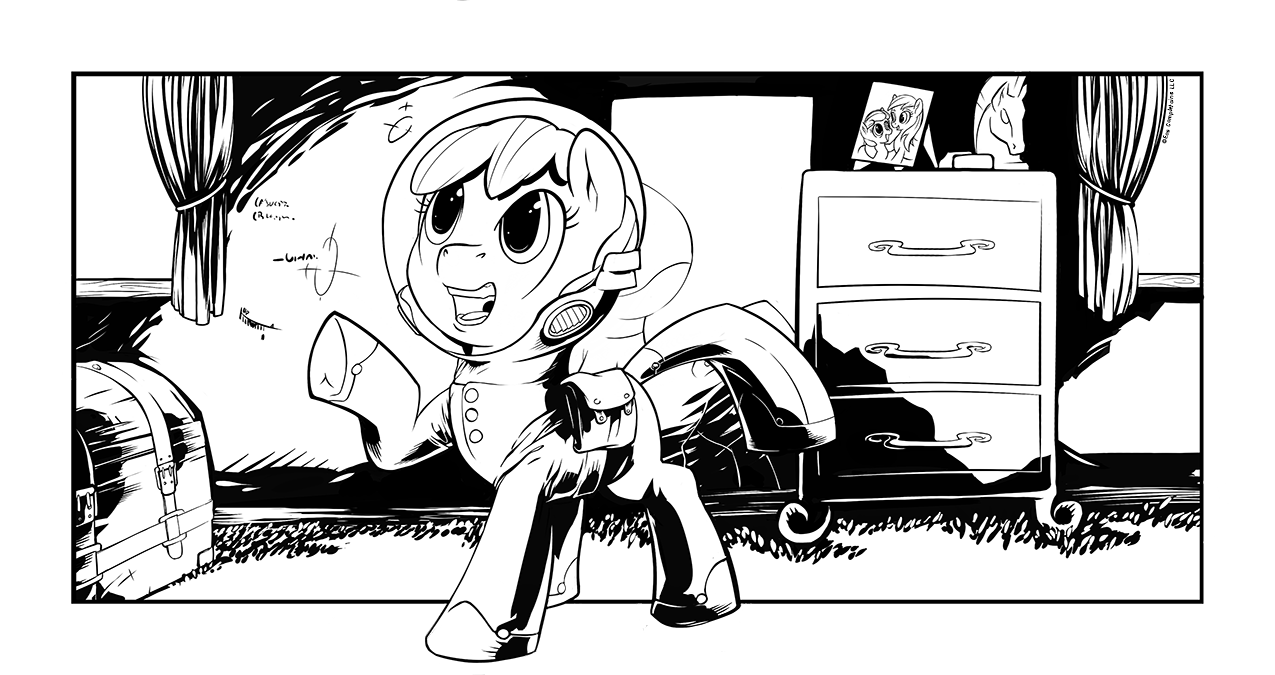
\includegraphics[width=0.9\linewidth]{image01.png}

\begin{intro}
Do you believe in ghosts?
\end{intro}


``Please, let us on!''

``The shield is failing; there's no time!''

A mass of ponies crowded in front of an air wagon. Everypony was jostling about, anxiously awaiting their turn to board, though the assigned pegasi were nowhere in sight. A green mare near the back of the crowd suddenly blurted out, shrieking. Desperately, she pushed ponies aside in a wild dash for the front.

``This is impossible! How can this be \emph{happening}\/? Celestia's abandoned us! Luna's abandoned us! There's n---''

\emph{BLAM!}

The mare fell silent as her body hit the ground. All eyes turned to a soldier who racked a fresh shell into her riot shotgun. 

``FORM A LINE AND WAIT YOUR TURN! THERE'S ROOM ENOUGH FOR EVERYPONY. TROUBLEMAKERS WILL BE MET WITH LETHAL FORCE!''

The towers of Canterlot overshadowed the hysterical crowd, observing the madness from afar.

\horizonline

Far above, in the streets of Canterlot, ponies scrambled wildly to find safety. Whole blocks were engulfed in fire, and many of the roads were blocked by upturned carts, crumbled buildings and fallen debris. Some ponies tried to help each other, struggling to clear paths and aid the injured.

In one crowded street, a group of stallions was attempting to breach a crumbled wall.

``One more time! All together now! \emph{Heave!}\/'' The ponies forced themselves upon the wall once again, desperately throwing their strength against it.

Finally, the wall gave way, allowing the group to filter through the opening. The road emptied, save for a young filly, oblivious of whatever was going on. She sat on her haunches in the middle of the street with her mane in her eyes, staring at the sky. Far above, a massive, shining bubble loomed over the city spires. As she watched, something hit the top of the shield and exploded into thousand colors.

``Oh, yay! Fireworks!'' she exclaimed gleefully.

``Hey, you there!''

A unicorn medical officer dressed in a white uniform had been hurrying down the lane,  distributing protective suits to the foals. Upon seeing the foal alone, she rushed over, casting her a concerned look.

``Are you alone? Where are your parents?''

The foal smiled back at the officer. ``Mom is up there!'' She pointed a hoof at the force field surrounding Canterlot. The energy bubble seemed a lot thinner than it was ten minutes ago. ``She'll be back for dinner!''

The officer hesitated, before looking at the foal and forcing a smile. ``Of course she will. What's your name, little one?''

``I'm Puppysmiles!'' cheered the filly, bouncing up and down on the spot.

``Yes\dots yes, Puppy, all right\dots Now, listen to me carefully. I want you to take this suit and put it on. You must wear the suit and not take it off, do you understand?''

The filly looked at the object with a puzzled expression, then at the white pony. ``Yes miss pretty pony! I like you!''

The unicorn smiled nervously, then levitated and unfolded the suit---it was lemon yellow, with several pockets on its legs and two saddlebags on the sides. 

``Okay, I need you to put your hooves into the holes for me. It's just like\dots like the pony pokey! Do you know the pony pokey?''

``Yush!''


\begin{song}
	``You reach your right hoof in
	
	you reach your right hoof out!''
\end{song}

``Right, that's perfect! Now the tail\dots here, let me close it up and put this on your head\dots there!''

The mare put a round, glassy helmet on Puppysmiles' head, then snapped shut a pair of locks on each side, finally sealing the small pony safely inside her radsuit.

``Woah! I look like a space pony! Like\dots like Captain Andromeda! Wooooosh!'' She started running and jumping in circles, giggling naively. The mare simply sighed in relief and turned towards the next group with foals.

Puppysmiles was having a super duper great time. Everything had begun with that huge boom. It had sounded like a super humongous party popper! Then the castle blew a gigantic-o-mongous bubble around itself, sort of like the bubbles her Mommy blew for her, only \emph{way}\/ bigger---and now everypony was in the streets partying. She prayed to her lucky stars that Mommy would come back home sooner today, so they could join in on the fun. The helmet and the space suit were just the icing on the cupcake: they were super cool and she was sure they made her look awesome\dots Right! What she needed now was a mirror! The filly dashed off toward her home.

\horizonline

The muffled street noise filtered into her mother's room. Puppysmiles stood in front of the dresser, examining her helmet from the inside. Strange lights and symbols danced across the glass. Several objects in the room were encircled in green halos and as she looked at them, in turn, writing appeared beneath. Too bad Puppy couldn't read. Her mom had barely taught her the basics.

``Buh\dots eh\dots duh.'' The filly wrinkled her brow in concentration as she constructed the word. ``BED! Wow, I'm good!''

Satisfied, Puppy trotted downstairs, completely forgetting about the mirror. Instead, she headed for the fridge.

``Muffins!''

Puppy promptly plucked one from the tray and went to take a bite. This immediately presented a problem---she couldn't get at it with that stoopid helmet on.

``Do want, but can't has\dots Bad helmet! How do I take you off?''

She grabbed the offending fishbowl between her forehooves and wrestled with it for a full minute, but to no avail. Panting, she sat down hard on her rump and decided to play her trump card.

``WAAAAAAaaaaahhhhhhh!'' 

Unnoticed by the yowling Puppysmiles, a red symbol appeared on her visor. Her tantrum was cut short by a robotic voice which began speaking from within the suit.

{\mt ``Status of the host: panic.''}

The filly blinked stupidly. What was going on? Who had spoken?

``Wut?''

{\mt ``Internal medical diagnostic initiated. Error! System rebooting. Estimated time: thirty seconds.''}

All those funny words were amusing, but they did nothing to rid her of the helmet. Puppysmiles was still upset.

``Go away stoopid talking space suit! I want muffins!''

{\mt ``Reboot complete. Checking version. Initiating. Ten seconds to full operational status\dots Eight\dots Seven\dots''}

In that instant, the noise outside surged---screams and howling cries filled the air. It sounded to Puppy as if all the ponies outside were singing.

{\mt ``Five\dots Four\dots Three\dots''}

Suddenly, the world went pink. Outside her mother's window, the foal could see the ensuing chaos. The cloud seemed to swallow everything. In an instant, the street, the houses, and all of the ponies were eaten. Oblivious to its meaning, Puppy watched on in awe.

{\mt ``Two\dots System rebooted. Starting diagnostic routine. Warning. Primary healing talisman is not responding. Activating backup healing talisman. Starting diagnostic. Female. Foal. Earth pony variety.''}

Wow, this space suit sure was smart! It knew a lot of things! 

``Hi, I'm Puppysmiles!'' she said.

A blanket of pink mist flooded the streets, muffling the sounds of the ponies it caught. Screams, whispers, and tears were all washed away as the cloud rolled on.

{\mt ``Life support online. Temperature within parameters. Blood pressure within parameters. Warning. Radiation level above the average by three hundred percent.'' }

Puppy giggled. ``Tee-hee, Mister Space Suit says fancy words!'' Puppy sat in front of the window, looking a bit puzzled at the mist leaking inside. She now wasn't sure of‒

{\mt ``Warning. Minor radiation poisoning detected. Inoculating: Rad-X. Inoculating: RadAway. Inoculating: Rad---}

{\mt ``Warning. Hazardous agent detected. Analyzing. Pink agent, Littlehorn type. Lethal at a concentration exceeding 5\%.''}

{\mt ``1.8\%\dots 2.0\%\dots 2.2\%\dots Warning. Concentration of pink agent above safety limits. Evacuate the area immediately.''}

Puppy stared in amazement as the pink fog oozed from the window and across the floor, smiling as it streamed between her hooves. It was like candy floss\dots pink candy floss! Yay! Her mom hadn't let her eat it since she made herself sick last Nightmare Night.

Suddenly, she felt her gut tighten.

``I feel funny\dots''


{\mt ``Danger! Mutation detected! Concentration of 5.4\%. Danger! 6.0\%! Evacuate immediately! Contact Ministry of Peace for immediate help! Initiating transmission of distress signal. Scanning for emergency channel. Transmitting. Warning! Concentration at 7.5\%!''}

``Ugh\dots Mommy\dots I don't feel very\dots good. Can I stay\dots home\dots tomor\dots'' Her eyesight was steadily growing hazy. She felt like she was sweating a lot, while at the same time she was freezing.

{\mt ``Inoculating: Med-X. Inoculating: Healing potion. Concentration at 12.1\%. Inoculating: Rad-X. Inoculating: RadAway. Concentration of pink agent at 16.0\%. Inoculating: Poison Antidote. Inoculating: Healing potion. Inoculating: Healing potion. Concentration at 22.6\%. Inoculating: Healing potion. Inoculating\dots''}

The ceaseless litany of the radsuit's medical systems continued as Puppy's legs gave out beneath her. Lying unconscious on the kitchen floor, the healing potions that coursed through her veins kept her alive. As the deadly pink agent slowly permeated the suit, the suit did its best to mitigate the worst of the effects. She did not die, but she didn't quite survive, either.

{\mt ``\dots Healing potion. Inoculating: healing potion. Inoculating: healing potion. Warning. Healing potion doses left: three. Concentration of pink agent at 35.0\%. Inoculating\dots''}

Like a lost doll, Puppysmiles lay silent as her suit sang its clinical chorus of programmed procedures: atmosphere toxic, suit compromised, medical supplies exhausted. She heard none of it as the minutes flowed into hours, hours into days\dots

She simply lay there on the floor, trapped inside a suit that endlessly informed her that she was near death and needed\dots practically everything.

Days became weeks and weeks became months as Puppy continued to sleep, frozen in that single instant of life.

Months gave way to seasons, and seasons to years, still the suit to sung its lullaby of medical emergencies.

Year after year, the voice of the suit grew lower and lower, beginning its descent into malfunction. Her helmet was covered in dust and soot, hiding the tragedies of the outside world from her sight as she napped on. Sealed inside her suit, her body twisted and broken, decades passed until they became a century\dots  then two.

The house bore the years without a single repair; it was a good house, built by earth ponies in the old fashioned way---brick by brick, with a solid roof and strong foundations. But all things must come to an end. It began as a little crack in the middle of the main roof beam during spring, growing larger and deeper with every rainstorm until the whole thing resigned to old age.

Right on top of Puppy.


\horizonline

\englishdaytimeplace{1}{5:00 P.M.}{Clover Leaf Terrace, suburb of Canterlot}

The building's collapse sent a plume of dust and pink smoke high into the air, and the resounding crash echoed through the city's desolate streets. As the debris settled, from beneath the ruins came a tiny, muffled voice.

``Owie\dots''

Slowly, a brick moved, followed by another, revealing something glinting in the rubble. A round glassy helmet popped up, followed by the yellow silhouette of a very small pony a radsuit. There was a long crack in the helmet, but somehow the damage began to disappear as the pony finished freeing herself from the collapsed building.

``Mom?'' The filly resembled an astronaut taking her first steps on an alien world. ``What is this place? Where is everypony? Mom? MOOOM?''

Something felt wrong, beginning with the fact that she was still wearing that talking suit.

``MOOOM!''

{\mt ``Bzzzt- FzZZzzZzt- line\dots rebooFZZZt necesszSzT!''}

``Shut up suit! Where's Mom? Where is my house? Where\dots am\dots'' The words caught in her throat as she finally realized where she was. An enormous mountain towered above her, topped by a ruined, but unmistakable castle; there was no doubt, this was Canterlot---her home.

``What\dots b-b-but\dots it's\dots all broken!''

{\mt ``Fzzzt\dots critical failure\dots no living parFZZZTT! Requesting conffFFZZZTanual rebooting.''}

``Yeah, whatever!'' she said, still gazing upward. All of a sudden she felt funny again. Her sight became foggy and she fell on her flank, her legs unable to support her. Puppysmiles grew weaker and weaker, feeling a terrible pain crawl from her hooves up to her spine. It was a new type of sensation---everything in her seemed to stop working. The more she tried to do something, the more she felt trapped. She tried to scream, but her mouth wouldn't move. The only thing left to her was staring down the empty street through a cloud of pain and a dusty helmet.

As she lay there, her focus shifted to a pile of strange, dirty white stones. Their shape was unusual: long and thin, some curved, some straight. Now that she was paying attention, she realized that they were everywhere. For some reason the sight of them strewn about disturbed her, but the sensation didn't last long. Suddenly, a green dot pulsed before her eyes, commanding her full attention.

{\mt ``Reboot complete. Checking version. File not found. Starting emergency mode. Version 0.2\dots''}

Puppy tried to say something, but her mouth wouldn't cooperate. The foal just stared at the weird lights in front of her eyes that flashed from green to pink. That was good news, at least. She loved pink!

{\mt ``New components detected. Initializing matrix. Connecting.''}

A spark ran through her body, zipping from her nose to her tail. It washed away the horrible sensation of paralysis. Hesitantly, she tried raising a hoof. It worked! It was as if the last five minutes had never happened. She just got better all of a sudden\dots Go figure.

``Wow, that was weird,'' she said, getting to her hooves. ``Now I just need to get this stoopid space suit off---''

{\mt ``All systems operational. Starting diagnostic routine. Analyzing. Subject 001, Puppysmiles. Female. Foal. Earth pony variety. No vitals. Checking for errors in diagnostic equipment. No errors found. Repeating diagnostic routine. Female. Foal. Earth pony variety. No vitals.''}

``What are whytles? I want whytles! Are they yummy?'' Puppy exclaimed.

{\mt ``Launching Learning Program for Foals. Connecting to Ministry of Image for recent updates. Unable to establish communication bridge. Launching program from backup files. Please wait for installation to finish.''}

Puppy began to skip around, testing her now unparalyzed legs. Eventually, she moved to a pile of old, weathered stones and stopped to get a better look at them. The HUD in her helmet illuminated the heap and surrounded its silhouette with a pink halo.

``Curly cuh\dots oh\dots ruh\dots puh\dots ss\dots eh! Cor\dots corrupse!'' She giggled: reading was fun! A second later, she frowned. ``What's a corrupse?''

{\mt ``Corpse, noun. Remnants of a dead creature--the more you know!''} the suit's metallic voice answered.

``Dead? Like\dots dead dead dead?''

{\mt ``Searching synonyms for dead\dots Cadaverous. Deceased. Defunct. Departed. Done for. Erased. Expired. Extinct. Gone. Inanimate. Inert. Lifeless\dots''}

Puppy listened for the first part of the list, then lost interest and poked at a long white bone with a hoof. She wasn't sure why, but something seemed familiar about this skeleton.

``Uhm, Mister Voice\dots this corpse\dots what was it?''

{\mt ``Analyzing: Pony---Unicorn variety. Adult female.''}

Puppy shivered, or at least felt like shivering. Her eyes rose, and she looked down the street littered with bones. Skeletons of dead ponies, curled in on themselves, lining the walls, and huddled into small groups, as if they had tried to find safety in numbers. And now they were dead. All dead.

``What\dots what happened? Mom? Where's Mom?'' Puppysmiles felt a cold sensation running down her spine. ``Mister Voice\dots where's Mom?''

{\mt ``MoM---Ministry of Morale. Analyzing data. Connecting to Equestrian Cartography Onspark. Downloading data. Error, name matching failed. Searching for MoM broadcasting signal. Spritebot found. Establishing communication bridge\dots ''}

Puppysmiles stopped following the voice after the first two or three sentences. Now she was trying to find her home. Maybe, just maybe her mother was there waiting for her!

``Why is everything different? Where is my house? Where are all the pretty ponies?'' She saw the rusted and battered remnants of the Pony Joe's Doughnut shop down the street, confirming that this was the street where she lived. Her house must have been\dots ``B-b-but\dots'' She stood in front of the ruins she'd crawled out of just minutes ago, looking at them in disbelief.

{\mt ``Query: broadcasting source. Broadcasting signal found. Location marker transmission in progress\dots''}

``If this is home\dots where's my mom?'' Puppy sat down and began to sob, or at she least tried to. It took her some time to realize that she was just bawling: no tears came from her eyes and she didn't feel relieved at all. Now she was almost sure that something in her was wrong. She was about to ask the voice about it, but was interrupted.

{\mt ``Ministry of Morale's locations added to map. Nearest MoM hub displayed on the navigator.''}

``Y-you found my mom?'' Puppy exclaimed, feeling a burst of hope.

{\mt ``Affirmative. MoM has been located. Nearest MoM hub outside Canterlot Ruins is set as new navigation priority.''}

``Uh\dots I\dots guess that's a yes?'' The filly tilted her head.

{\mt ``Instructions: follow the pink arrow on the compass until destination is reached.''}

``Uh\dots thanks?'' It took her a moment to realize what had just happened. The voice had just found her mom! Who cared about the house, the dead ponies, the ruined castle or this stoopid\dots no wait! This super duper smart space suit was going to bring her to mom! The thought overwhelmed her with glee. Who cared if she didn't feel hungry or tired or whatever, Mom would know why! She was going to find her mom, so everything was going to be fine!

 ``YAY!''


\horizonline

\englishdaytimeplace{1}{8:30 P.M.}{Sunshine Plaza, outskirts of Canterlot}

{\mt ``Warning. Vital parameters absent. Warning. Medical supplies exhausted. Warning. All emergency channels are mute. Warning\dots''}


\begin{song}
	``Warning wrap up warning wrap uuup!''
\end{song}

Puppysmiles was trotting down the streets of Canterlot's suburbs, singing her own version of the greatest song ever in all of Equestria. She tried to match the suit's droning so that they seemed like a chorus.


\begin{song}
``The medical supply's tired!

Warning wrap up warning wrap up!

We'll soon need batteries!''
\end{song}

{\mt ``Negative. Energy supply is sufficient. Estimated lifetime of the spark before red level: one thousand, two hundreds years.''}

``Oh come on! Just sing and stop whining.''

{\mt ``Negative. This is not whining. This is a warning. I can supply appropriate audio samples of whining.''}

``Warning for what? Everything will be all right as soon as we find my mom! She's the coolest pony ever!''

{\mt ``Negative. MoM is not a pony. It is an acronym for---''}

``Of course Mom's a pony\dots and she's not an\dots uh\dots an acrobat either!''

{\mt ``Negative. MoM is Ministry of Morale.''}

Puppysmiles giggled. ``Silly Mister Voice! Sticks and stones may break my bones, but words will never hurt me!'' She giggled again. ``Ministry of Morale, as if that has to do with anything.''

Puppy trotted down the deserted road, passing many places familiar to her. As daylight faded into dusk, she found herself in a large city square before a statue of Princess Celestia. ``Wow, pretty Princess Celestia\dots when I'm big I want to be a princess too!''

Puppy paced around the monument with curiosity, trying to find a way onto the statue's back. Having a ride on a gigantic marble Celestia seemed just too awesome to be a bad idea, but as she prepared to begin her ascent, the suit interrupted.

{\mt ``Warning. Hostile detected. Distance: twenty meters. Analyzing\dots''}

A red dot appeared on the compass beside her pink objective. Turning to face it, she saw a pony watching her from the doorway of a post office. At last, somepony else! What's-his-name, Horse Tile? Tee-hee, that was a funny name! She skipped toward him with her best winning smile.

``Hi Mister Horse Tile! I'm Puppysmiles!''

{\mt ``Warning. Hostile at six meters and closing.''}

``Oh, and this is Mister Voice! He lives in my space suit and whines all the time, but he's super smart!''

The creature stared at Puppy with an empty, glowing gaze. He was a horribly disfigured earth pony---his mane was almost completely gone, and skin peeled off his body in several places, revealing rotting meat and yellow bones.

``Gwaah\dots'' he growled and took a step towards her.

``Uhm\dots is something wrong with you, Mister Horse?''

{\mt ``Analysis complete. Creature: Canterlot feral ghoul. Threat level: lethal. Tactical retreat is advised.''}

Puppy stopped, transfixed by the ghoul's unwavering gaze, suddenly aware of the horror standing before her. The ghoul simply stood and stared back.

``I-forgot-something-very-important-sorry-gotta-go-okay-bye-bye!''

The foal turned and sprinted for her life, scrambling over bones and screaming like the scared little filly she was. \emph{``Ayeeeeeeeeee!''}\/ The ghoul watched her display until she disappeared from sight, then sauntered back into the post office.

After several blocks, Puppy finally decided it was safe to slow down and catch her breath. She looked over her shoulder, hoping the monster had given up the chase. The street was empty. Lucky Puppy! She was best runner ever! Maybe she could even do a sonic rainboom without even flying! Was that possible? It would have been super cool for sure\dots ``Okay Mister Voice\dots you're the egghead. Is that not-so-pretty-pony still chasing us?''

{\mt ``Negative. Scanning shows no activity in the area.''}

``Super\dots now let me just catch my breath then\dots we'll\dots'' Puppy realized something strange. She was barely winded despite having just run half a kilometer at full gallop. She had only stopped because she felt that she \emph{should}\/ be tired. Something about that seemed a teeny tiny bit wrong, and it made Puppy recall all the warnings the suit had been giving her\dots Maybe there was something that she needed to know.

``Uhm\dots Mister Voice\dots am I ill?''

{\mt ``Running diagnostic procedure. Please wait. Negative. The subject is not ill, wounded, or poisoned.'' }

Puppy felt relieved: the thing about not being hungry or tired was probably nothing unusual. Her mom was always awake after Puppy's bed time, and she never got tired. Maybe she was growing up at last? Yush! Puppy was becoming a big pony like Mom! 

{\mt ``Diagnosis complete: the subject is deceased.''}

``Diseased? You just told me I was all right!''

{\mt ``Negative. I said that you were not ill.''}

She frowned. ``Waaaait just a moment. I'm not ill, but I'm diseased?''

{\mt ``Negative. You are deceased.''}

``But that's what I just said!'' She stomped her hoof.

{\mt ``Negative. The word you are using is incorr-''}

``Aw, just stop with this. I say tomato, you say \emph{tomahto}\/! You don't want to tell me what's wrong? Fine! I don't want to know! Bleh!'' Puppy stuck out her tongue at the helmet HUD and once more started to follow the pink compass heading. She had barely noticed that night had drawn in around her; she could still see everything as though it were day. Unbeknown to Puppy, her eyes now shone with a faint pink light.


\horizonline

\englishdaytimeplace{1}{10:00 P.M.}{Dead Hills, Wasteland}

As Puppy made her way out of the city, she found herself overlooking a huge valley. As it stretched into the distance, she saw it pass through a desolate landscape of scorched hills and dead forests with little sign of civilization in between. Puppy slowed to a stop and looked around, confused.

``Hey, Mister Voice\dots are you super duper sure that this way is okay? We're not heading anywhere near the mountain top\dots''

{\mt ``Affirmative. The nearest likely-intact MoM hub is located in this direction. However, it is not currently broadcasting. Other hubs are also located further down this route.''}

The filly frowned for a moment, straining to understand what the suit had just said. In the end, she simply smiled. ``Okie dokie lokie\dots let's sing something then!''

\begin{song}
		``There, is a place, where the grass is what's for dinner!
	
		Charmed, fun and wild, there must be something in the water!''
\end{song}

\horizonline


In the Wasteland, walking down the road making as much racket as she was is just asking for trouble. Within half an hour, Puppy had attracted the attention of every potential aggressor in the area, though most of them were a bit wary of how to proceed.

{\mt ``Warning. Several hostiles detected. Caution is advised.''}

``Wut? Mister Horse Tile again!?'' Puppy looked around in a frantic panic. She was sure that she'd lost him in town, how could he---BLAM!

She fell to her rump as a stinging pain in her left hind leg made it buckle. The pain wasn't that bad, but for some reason she couldn't get up.

``Owie\dots''

Puppy looked up from her injury to see a group of ponies rushing wildly toward her.

``I hit it! Go, kill it- \emph{kill it}\/!'' One of the ponies shrieked.


``You! I'm gonna eat your heart! GRAAAAH!''

``I want his helmet. It's mine, I saw it first! It's mine it's MINE! He's not bleeding! Why isn't he bleeding? MAKE HIM BLEED!''

{\mt ``Warning. Breach in containment layer. Exposure to external elements unavoidable. Survival of subject not guaranteed. Self repairing magic activated.'' }

Puppy waved a hoof at the new arrivals. ``Hi pretty ponies! I'm Puppysmiles! Have you seen my Mom? Oh, and watch out for the horseflies! They sting like crazy!''

She just sat smiling at the three ponies, trying to behave and ignore the annoying sting in her leg. Stoopid insects. The trio of ponies charging toward her showed no signs of slowing down. She frowned. ``Is something wrong?''

``Immobilize that bastard! Cut his fucking legs off! I want to see how he does as a snail!''

One of the three, a large, muscular earth pony, tackled Puppy to the ground, effectively burying her under his bulk. The other two split up---the unicorn kept his distance and trained a rifled at the foal's head, while the second earth pony, a mare, pinned Puppy's legs and withdrew a wicked-looking knife.

``Got you! Now, hold still while I---''

{\mt ``Warning. Pink agent, Littlehorn Type detected.''}

As the second earth pony landed on Puppysmiles, a thick pink cloud gushed out from the bullet hole in the suit, puffing right into the muscular pony's face. At first the stallion looked annoyed, but his annoyance was quickly replaced by realization, and then terror as his face began to boil.

``WAAAGH! EAUGH! HELP ME! \emph{HELP ME!}\/''

The other two raiders stared in disbelief at the massive earth pony as his face melted and dripped from his skull like ice cream on a hot summer's day. The earth pony mare looked at the filly inside the helmet. She seemed so small, so innocuous\dots \emph{she had big\dots pink\dots glowing eyes}.

The mare gasped. ``It's a ghoul! Back off! Back o‒'' Suddenly, she coughed up blood. She squirmed, trying to flee, but it was too late to run. She had already tasted the pink venom, and without a healing potion she was just as dead as her companion.

The unicorn screamed in terror, threw the rifle against Puppy's helmet, and then ran for his life. In the meantime, the big male rolled from Puppy's back as liquefied brain leaked from his skull and splashed onto the asphalt. The female hardly made it far. Choking on her own blood, she managed to get about a hundred meters before collapsing.

{\mt ``Warning. Breach in the containment layer. Exposure to external elements unavoidable. Survival of the subject is not guaranteed. Repairs in progress.''}

Puppy was reeling, shell-shocked by the big pony's death\dots it was more horrible than anything she'd ever seen. What in Equestria could have done that? Melting a head with all the skin and the bones and\dots suddenly she realized. ``Mister Horse Tile! He had the same melted face! He killed them!'' And now she was next! No\dots no, no, no, no! That wasn't good, she had to get up and run away, run away \emph{fast}. Unfortunately, her leg wasn't cooperating. She tried to get up and run but could barely manage a stagger, so stagger she did.

{\mt ``Repairs completed. Containment restored. Running medical diagnostic. Subject deceased.''}

``Don't you dare start that again! We're in a pinch here!''

{\mt ``Negative. No immediate threats detected. Hostile count in the area: zero.''}

``Count? Mister Horse Tile is a noble pony?''

{\mt ``Negative. The correct word is hostile. You are distorting the meaning of-''}

``What are you, a dictionary? I'm tired of your fancy words!'' Puppy sighed with frustration. ``Look, there's a super-evil zombie pony count after us and we have to get out of here before he finds us again!''

{\mt ``Negative. You misundersta---''}

``CUT! IT! \emph{OUT!}\/'' She seethed. As anger grew inside Puppy, her eyes flared, becoming as bright luminescent. The twin flames were so bright that she could see herself reflected in the glass of her helmet. That vile-looking monster staring back at her---Was- was that her?

Speechless and completely lost in the vision, Puppy fell to the ground. She clutched the helmet between her hooves, closed her eyes and started to cry. There were no tears, but it was loud---a soul-felt wail that echoed through the wasteland.


\horizonline

\englishdaytimeplace{2}{6:45 A.M.}{Dead Hills, Wasteland}

Through the night, many creatures heard her cries and ventured to investigate, though none of them drew too near to her. There was something about the filly that disturbed them.

It was nearly morning by the time Puppy stopped crying; light was just peeking up over the horizon. Slowly, she lowered her hooves from the helmet and opened her eyes. The suit had been mute since her little scene the previous night, and she now felt lonely.

``Uh\dots Mister Voice\dots are you there?''

{\mt ``Affirmative. All systems are powered and ready.''}

``Ah\dots right\dots I\dots I just wanted to say that I'm sorry\dots I didn't mean to shout at you. I\dots''

{\mt ``Warning. This program is not designed for socializing. The emergency mode only provides hardware support, voice command interpretation, and basic survival advice.''}

``I\dots please\dots please, please, please, don't leave me alone! I'm sorry! Please take me to my mom!''

{\mt ``Location MoM already set as priority navigation point.''}

Puppy hesitated for a moment, trying to understand what the voice was implying. ``Uhm\dots are you saying that we are still going to find Mom together?''

{\mt ``Affirmative. It is the set priority.''}

``YAY! I love you Mister Voice!'' Puppy was suddenly interrupted by the sound of a manly metallic laugh, but it wasn't coming from inside her helmet. The filly looked around, trying to pinpoint the source, and found a spritebot fluctuating in the air behind her.

``Uh\dots hi? I'm Puppysmiles\dots'' After her last experience with newcomers, she wasn't completely sure that the \emph{everypony is a welcome pony}\/ approach was the best one, but she had been told to be nice and she didn't want to disappoint her mother.

The spritebot hovered for a few moments longer, then replied, ``Oh, hi, Puppy\dots can I call you Puppy? You're quite an interesting encounter.''

Puppy smiled happily. A friend at last! ``Sure! Everypony calls me that. What's your name, buzzing eye?''

``I'm Watcher, pleased to meet you.''

She tilted her head. ``What are you watching?''

``Well, anything that I find interesting.''

``Wow, that must be a lot of things!''

The bot laughed for a moment. ``Well, yes, quite a lot\dots Say, is that a fully functioning Mark VI Omni-Environmental Suit you're wearing?''

``Nope, it's a space suit! It's super cool and it also talks, but I can't get out of it.''

``Oh, and how did you get inside it?''

``A pretty pony put it on me yesterday.''

``Yesterday? Can I ask who that pony was?''

Puppy pondered for a moment. ``She had a pretty white vest and made me sing the Pony Pokey\dots it was all a bit crazy, and she didn't tell me what her name was\dots''

``Crazy? Like what?''

She frowned, trying to remember the important details of the encounter. ``Well, there was this big bubble all around the castle and the streets were full of ponies and soldier ponies and then all that pink mist and-''

``Woah, slow down for a moment! Pink mist? Castle? Do you mean in Canterlot?''

``Yup! Well\dots not \emph{Canterlot}\/ Canterlot\dots we live downhill, but it's still Canterlot, you know?''

``Yes, I\dots I know\dots'' the voice hesitated. ``And\dots this happened yesterday?''

``Uh\dots maybe it was a couple days ago\dots yesterday I woke up and all the pretty ponies were gone and\dots ah\dots my house was gone too and\dots there were lots of corpse ponies and it was creepy\dots and a really ugly pony chased me but now it's okay because me and Mister Voice are going to find my mom!''

The spritebot was silent for a long time. Puppy just kept smiling, waiting for her new friend to say something else. When the voice finally came back, it sounded distant and somehow not so friendly.

``So, after the thing with the pink cloud, you went to sleep and you woke up the next day and everything was just\dots gone\dots''

``Eeyup!''

``And\dots you've not been able to get out of the suit since then and\dots you haven't had to drink or eat or\dots go to the restroom?''

``Nopey mopey.'' The filly smiled. ``Mister Voice said it was because I was diseased but then he said no and then yes and we had this big argument about fancy words.''

``And\dots can I ask you where you are going right now?''

At last, an easy question! ``Sure! I'm going to find my Mom! Mister Voice found her and I'm following this super nice pink arrow! When I find her everything will be all right!''

``This\dots Mister Voice\dots pointed you in that direction? Down this road?''

``Yes! Wow, Mister Watcher, you are super curious, aren't you? You should be called Mister Questioner!'' She giggled, the voice didn't say anything for almost a minute.

``Oh Celestia I\dots I can't. Listen, Puppy, I\dots''

``Yes?'' Her eyes grew bigger.

The voice went mute again for a long while. ``I'm sorry, I have to go. I\dots I wish you luck.''

``Sure! Good luck to you too! When I find my mom I'll tell her that you were nice to me! Bye bye!''

The spritebot gave a brief burst of static and began playing some music, floating away in the direction of Canterlot.

``Wow, music! He has music! Cool! Hey Mister Voice, do we have music too?''

{\mt ``Affirmative. I receive several radio signals. Some of them are meant for entertainment.''}

Fancy words again. Puppy frowned trying to translate that sentence. ``Uhm\dots this means we can has music?''

{\mt ``Affirmative.''}

``Hit it!''

After a few crackles of static the radio began playing. Puppysmiles continued south, trotting merrily along the lonesome road.


\begin{music}
		What is this place
	
		filled with so many wonders?
	
		Casting its spell
	
		that I am now under\dots
\end{music}

\clearpage

~\vfill

\begin{engnote}
level up\dots No wait, Puppy uses a monster template! Does she get lvls? I think not.
\end{engnote}

\engprintstatus{5}{4}{5}{7}{4}{6}{9}


\chapter{Party Hard}

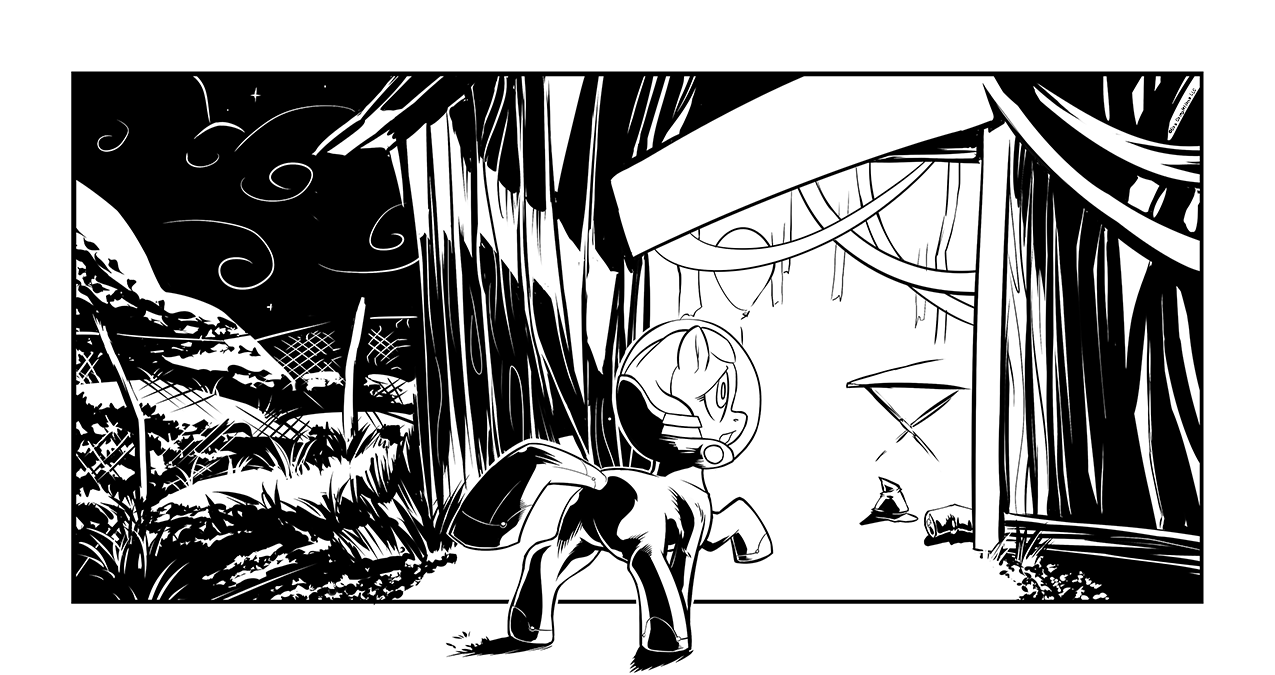
\includegraphics[width=0.9\linewidth]{image02.png}

\begin{intro}
No need to bring a gift, being there will be enough!
\end{intro}

\englishdaytimeplace{2}{4:00 P.M.}{Redtrotters Ridges, Big 52, N. Branch}

Usually, wearing a full environmental suit is not considered the cutting edge of Equestrian fashion, but anypony has to admit that it brings some neat advantages. First of all, if you were to survive a direct hit from a balefire bomb, you'd probably live long enough to die of thirst inside the suit before the radiation got you. The other good thing about being inside a hermetically sealed, radiation shielded suit is you'll never want for an umbrella or sunscreen again. And being lemon yellow, it's nearly impossible to go anywhere unnoticed unless, perhaps, you've been buried under an avalanche of lemons. Obviously there are moments in the Wasteland where stealth is a virtue.

As if Puppy even knew the meaning of the word.


\horizonline


``Hi! I'm Puppysmiles!'' She beamed at the two new ponies in front of her. Their uniforms, if they could be called that, resembled the trio from the other night's, but seemed cleaner and less ragged. One, a unicorn mare, scanned the road behind Puppy with her caravan shotgun, searching for what was to her an obvious ambush. Beside her, her earth pony partner kept a large spear levelled at Puppy. Had the foal been a wiser pony, the two mare's actions might have worried her.

The unicorn was the first to talk. ``What are you doing in Redtrotter territory, foal?''

``And what the hay is that weird suit?'' added the earth pony.

``I'm looking for my mom!'' Puppy replied enthusiastically, pointing a hoof more or less in the direction the road was going. ``She's that way!''

The two tribe ponies exchanged a glance before the unicorn spoke again. ``Okay, and what's your mother's name? Is she a Redtrotter?''

``What's a Redtrotter?''

The unicorn, her unease flaring into anger, prepared to go ballistic on Puppy. Sensing this, her partner stepped in. ``We are the Redtrotters. We control the Transequestrian Route 52 from here to Salt Cube City. If you have business on the Big 52 you do it through us. So, what's your mother's name?''

``My mommy is called Rainy Days! She's super cool and she always sings for me and she's a great cook too! She's the best pony ever and when I'm big I want to be like her!''

``Yeah, all right kid, I get the point,'' snapped the unicorn. ``I don't know a Rainy Days, so she's definitely not a Redtrotter. Are you alone? Who sent you here?''

``Mister Voice is with me!''

``Mister Voice?'' The unicorn warily surveyed the road again.

``Yeah! He lives in my space suit and sometimes we sing together but sometimes he gets grumpy but it's okay because he's helping me find Mom!''

\emph{``Right.''} The mare lowered her guard. ``Look, I'm sorry, but if you and your invisible friend want to pass through here, you need to pay the fee.''

``Ah, okie dokie? I have\dots'' Puppy started searching the many pockets of her suit. She had amassed a small hoard of junk in her short travel, mostly broken toys and things she thought were interesting. Maybe she had something these ponies would like. After all, \emph{you gotta share, you gotta care,} right?  ``What about this?''

Manipulating things without her teeth was quite a problem. She had to use her hooves instead. This task was only made more difficult by her bulky rubber boots, and the fact that she had to bend her leg at an awkward angle in order to reach into her saddlebags. ``Just a minute, I've almost got---no, uh.''

{\mt ``Assistance. The suit is equipped with a weak manipulation spell. Access your Inventory from the HUD and ask for the required item.''}

``Wut?''

The earth pony watched as Puppy mumbled to herself while fumbling out various useless junk from her saddlebags. The filly obviously couldn't pay. The spearmare looked at her friend and caught a meaningful glance. She sighed wistfully and after a brief internal prayer to the cruel gods of fate, plunged her spear into the foal's neck. Puppysmiles was so busy listening to the suit that she never saw it coming. She dropped to the ground like a sack of bricks, the earth pony letting her fall, silently cursing the Wasteland.

``You did her a favor. She wouldn't have lasted a day without her mother, and we can't afford to take her in. Better that we made it quick then let her get eaten by a manticore, or worse. You know what happens to foals around here,'' the unicorn trailed off with a sigh.

The earth pony noticed the troubled expression of her companion. ``Yeah. Poor Ridge Racer.''

The spearmare retrieved her weapon from the body. As she stepped back, pink smoke began to escape from the hole in the suit. The mare stared at the phenomenon, puzzled. ``Hey, Boney, what's that?''

The unicorn scratched her head with a hoof. ``You must have broken some talisman in the suit. It could be poisonous. Best to stay back.''

``We can't just leave her here, it doesn't feel right.'' The earth pony hesitated, trying to keep away from the pink smoke.

``After that funky little smoke show, I'm not going near her! The radroaches can take care of it. Come on, we still have a patrol to finish.''

With a final look at the fallen foal, the two mares trotted away, leaving the main road before climbing over a low ridge and out of sight. Time passed as the body of the filly in yellow lay alone in the middle of the road. A cold breeze picked up, rustling the bare trees. Despite the wind, the pink cloud that surrounded her did not seem to dissipate.


\horizonline

\englishdaytimeplace{2}{4:30 P.M.}{Redtrotters Ridges, Big 52, N. Branch}

The first sign that the lance had failed in its purpose was the automated speech of the suit coming back to life with a series crackles.

{\mt ``Initializing system. Checking version. Warning. Version number not corresponding. Starting in emergency mode. Version 0.2. Checking equipment status. All systems online. Major breach detected. Repair spells activated. Resuming last session. Loading personal data for subject 001: Puppysmiles. Subject deceased, condition stable. All clear.''}

Puppy's eyes began to blink for a moment inside the helmet, as if she had just awoken from a pleasant sleep. The foal yawned and a droplet of pink, glittering fluid fell from her mouth and onto the helmet of the suit, disappearing almost immediately as it was absorbed by the glass.

``Uhm, five more minutes, Mom.'' She turned around, still surrounded by the pink cloud that was now slowly fading.

{\mt ``Breach repaired. Subject insulated from external environment.''}

Lazily, Puppy got up and looked around. She frowned at the unfamiliar settings for a few moments before her memories came flooding back. ``Oh, right, Mom's not here. What was I doing before going to sleep?'' Puppy tried to scratch her head, but her hoof found the helmet on its way. She frowned again, then shrugged and continued to scratch the helmet thoughtfully.

{\mt ``Retrieving temporary memory. Query: last performed action before losing senses---negotiating passage.''}

``Negotiating what?''

{\mt ``Interacting with self-proclaimed Redtrotter ponies.''}

Fancy words again. ``Red-who?''

{\mt ``Talking with the pretty ponies.''}

At last, something comprehensible! ``Oh, right, pretty ponies! Now I remember! Ah, where have they gone?''

{\mt ``Location of Redtrotters unknown. Adding `Find the Redtrotter's' to the active mission list.''}

Puppy raised an eyebrow with a stumped expression. ``We have a to-do list? Since when?''

{\mt ``List initiated 23 hours ago. Objectives on the list: four.''}

``Wow, we have a lot of things to do! Four is a lot, right? What's on the list?''

{\mt ``Main objective: Reach MoM. Secondary objective: Get rid of space suit. Secondary objective: Confront Count Horse Tile or continue avoiding him. Secondary objective: Find the Redtrotters.''}

After listening to the list, the filly in yellow tapped her helmet with a hoof, a thoughtful expression on her muzzle. ``Think, think think. Muffins! No wait, that wasn't it.'' 

After several minutes of thinking, the foal finally nodded, a new resolve shining in her eyes. ``Okie dokie, play some music. Ah, the one with the chatty pony.'' Puppy trotted along the road, following the arrow and listening to the radio with a spring in her step.

The area surrounding Route 52 was a scorched wasteland dotted with rocks and ridges. It was hard to see very far because of the irregularity of the terrain. This normally would have been a problem, had Puppy any sense about her.

``Hey, Mister Voice, did you say something about taking stuff from my pockets?''

{\mt ``Affirmative. This suit is equipped with a weak manipulation spell.''}

``Uh, how does it work?''

{\mt ``Loading instructions. Selecting easy version for foals and Derpy. Name the object you need. If it is in your possession it will be put in front of you.''}

``Ah, muffins!'' A box of two hundred year old muffins floated in front of Puppy. She giggled. It looked so silly hovering in the air like that! ``Hey, this is fun! Sarsaparilla!'' A bottle of sarsaparilla replaced the muffins. ``Toy cart!'' This time a small toy cart in poor condition floated in front of the foal. ``Tee-hee! We need more stuff, I like this guessing game!''

{\mt ``Negative. This is not a guessing game. It is inventory management.''}

Puppy took a rock and put it in her pocket. ``A rock!'' The rock floated out of the pocket and listed lazily in front of her. ``Yay! It works!'' When it was put away again, the stone was labeled \emph{The Rock Of Destiny}, but since Puppy was not so good with reading, she didn't notice.

Trotting down the road, the filly kept asking for everything she had in her backpack, which really wasn't very much. She only owned four objects, but she planned on changing that soon. ``Oh, and we need more music!''

\begin{music}
		I can see that lone star from a thousand miles away
	
		Calling me back home, though I ventured far astray.
	
		When I see that beacon shining for me all alone,
	
		It calls me back to `Questria and my home!
\end{music}

\horizonline


\englishdaytimeplace{2}{7:00 P.M.}{Redtrotters camp, Big 52 N. Branch}

The Redtrotter's settlement was little more than a dirty bunch of half ruined shacks encompassed by a moat. Its barricade looked more like the result of a road crash between some old carts rather than a purposefully-built defence. Puppy was blissfully unaware of all this as she kept trotting toward the town, singing along with the radio until the road in front of her suddenly exploded into a shower of dust.

``Hey! I told you to STOP! RIGHT! THERE!''

Puppy looked toward the barricade and could see that there was a pony some fifty meters away. He was aiming a stocky gun at her. The filly sat down, waved a hoof and smiled. ``Hi! I'm Puppysmiles!''

The pony with the hunting rifle, who was peeking from behind the barricade, didn't seem very impressed. ``Okay, take that goldfish bowl off and show your face!''

``Uh, I'd totally do that if I could, but I'm stuck inside!'' Puppy pondered for a moment. ``Actually, it's on the to-do list!''

``Great, just great. Now, stand there where I can see you, and put down all of your weapons.''

``I don't think I have any weapons with me. I have a rock, does it count? I can throw it!'' She offered with enthusiasm.

The guard pony facehoofed. ``Hey, Doublesize, go and search her! You with the yellow suit, just stand there and behave!''

``Okie dokie lokie!'' Puppy smiled, but for some reason her answer startled the pony behind the barricade.

``Just say okay, don't try anything \emph{fun} and maybe nopony will get hurt! Do as I say now. Don't resist and let Doublesize do his work.''

A big, brown unicorn stallion approached Puppy, looking at the smiling filly through the glass of her helmet. The light was beginning to fade and now her eyes were just a bit pinkish, although it was hard to see thanks to all the equally pink lights coming from the helmet's HUD.

``Wow, that's a mighty fine radsuit you have there. Never seen one like this before.''

``Yush! It's super yellow and it's smart and it can do magics! Look! Look at this! A-hem. Muffins!'' The muffin box from before levitated in front of Puppy.

``Wow, integrated inventory management and lesser manipulation spells. This thing must cost a fortune. Where did you find it?''

``A pretty pony gave it to me in Canterlot!''

``So, you're from Canterlot?'' Doublesize gave a slight frown and shook his head.

She nodded proudly. ``Ah-huh!''

``The place with a big castle on the top of a mountain right at the beginning of the Big 52?'' 

``That's it!'' replied Puppy, smiling.

``Wow, that explains why you're wearing a full environmental suit at least. Okay, let's get back to business. Show me your pass.''

Puppysmiles stared blankly at the brown unicorn. ``My what?''

``You don't have a pass? Didn't you meet a patrol on the road coming here?''

``I met two pretty ponies. One was an earth pony like me and the other was a unir-unisc-unicron! They were super nice and super pretty!''

``Yes, yes, Rattling Bones and Frozen Soda,'' said Doublesize, cutting her short. ``Didn't they say anything about a passage fee?''

``Uh, I don't remember. We were talking for a bit, then they went away and left me alone and sleepy.''

The unicorn sighed and called for the pony at the barricade. ``Hey! The foal's clean, but it seems that Boney and Soda are giving out free passes today! The kid met them but she has no pass. What now?''

``Just take items from her that's worth the ticket and give her a pass!''

``Uh, okay.'' The earth pony stripped Puppy of everything she had but the rock and the suit. He tried to unlock even that, but the harness seemed to be sealed shut from the inside. ``Oh well, I guess it's just how things go. Sorry kid.'' He gave Puppy a flattened tin can with a red stain in the middle. ``Here you go, special discount for foals.''

``I'm telling my mom that you've been nice to me! Thank you mister pretty pony!''

``Oh, right, speaking of that, what's a foal in a rad suit doing all alone on the Big 52? This isn't a nice place.''

``I'm going to see my mom!'' Puppy took a look around as if she was trying to align herself with some invisible mark, then pointed a hoof toward a high ridge to the southeast. ``There! Okay gotta go bye bye!'' Without waiting for a response the foal merrily trotted away.

``But the only thing in that direction is the Carnival. Wait a second, kid! It's dangerous business going out there!'' Doublesize raised a hoof, but stopped himself. This was the wasteland and she wasn't family, so why bother? 

The filly in yellow wandered off the beaten path and explored among the rocks and the ridges. She found some sort of track, a winding trail running up and down the landscape just as if somepony had gone around dragging a couple of pointy sticks over the ground. Puppysmiles sniffed for a moment at the trails before ignoring them; for the foal climbing rocks and jumping from stone to stone was a super fun game; so, with \emph{a hop, a skip and a jump}, the evening became night as the foal ventured deeper and deeper into the wastes.


\horizonline

\englishdaytimeplace{2}{10:30 P.M.}{The Carnival, Wasteland}

A large barn stood at the bottom of a narrow valley, its once friendly coat of pink paint now faded and cracked. It was protected by a fence that ran all around the surrounding ridges, with automated turrets placed at fairly regular intervals. The building and the fence were in bad shape, and so were the turrets, but, despite their damage, several of the guns continued to slowly sweep side-to-side, guarding the perimeter.

{\mt ``Warning. Automated point defense turrets detected. Turrets are set on hostile mode. Threat level: medium.''}

The word hostile immediately put Puppy on alert. She stopped for a moment, looking around at her surroundings. ``The Count again? Where? That pony is persistent. Uhm, better safe than sorry, I guess.'' The little pony hid herself behind a rock and waited to see if Count Horse Tile was up to any mischief. ``Shush the music, Mister Voice, we're hiding.'' She held her breath and strained her ears to hear if somepony was moving.

{\mt ``Establishing communication bridge with the defense system. Exchanging protocol. Asking for clearance. Permission granted. The way is clear, please proceed.''}

``Shush, I said! There must be somepony here. It could be the Count! We have to be super sneaky.'' Puppy crawled out from cover and glanced over her shoulder in case somepony was creeping up behind her, before slowly moving toward the fence. The turrets almost immediately pointed in her direction, but their dots on the compass changed from red to pink and the guns returned to their default positions.

``Hey, Mister Voice, I told you to stop the music!''

{\mt ``Affirmative. The radio has been muted.''}

``So why do I keep hearing music?''

{\mt ``Sound source detected. The music is coming from inside the MoM building.''}

``From inside? Mom's inside that barn? With the music and everything else? Mom is throwing a party? YAY!'' Puppy instantly stopped hiding, got up on her hooves and ran downhill straight to the barn doors. When the filly arrived she bucked open the doors, jumped inside and yelled, ``SURPRISE!''

The barn's inside consisted of a single large hall with two open lofts, one right above the entrance and the other on the opposite, short side of the structure. The floor was made of flattened and pressed ground, covered sparsely with hay, and the walls were decorated with old streamers and garlands. From the ceiling hung some sorry-looking piñatas, a lot of limp, deflated balloons, and other old and half-destroyed decorations. The barn was sparsely lit by a couple of flickering lamps. The only thing that seemed to work properly were the speakers that were playing music at an almost deafening volume.

Right in the middle of the room there was a long table prepared for a party, with colored dishes and plastic glasses with names and everything else. There were plenty of guests sitting at the table: a bag of flour, a pile of rocks, a bucket filled with some unrecognizable liquid, and a chunk of dust, all of which wore a party hat. No less than a dozen lifeless, skeletal little ponies sat around the table, wearing festive party hats and staring blankly into empty plates. There were even a couple of corpses that looked more like mummies than skeletons. One of them might have passed for a very hungry pony. A large pile of white bones lurked in a far corner of the barn.

{\mt ``Warning. Mild radiation detected. Warning. Contaminating agent detected in the air. Analyzing. Nitrous Oxide. Threat level: negligible.''}

``Oh look, a new guest!'' A figure rose from its seat as the guest of honor. It was a pony with a staticky, fizzling voice that sounded like an old vinyl. In the dim light it looked like it was just a pink pony with an even pinker mane, but when it approached, Puppysmiles noticed that it was moving on a set of wheels, like it was wearing motorized roller skates. ``Well well well, look at you! I guess you're here for the masquerade! I'm super sorry to inform you that it was canceled, but you can keep the costume! It rocks!'' Usually, ponies moved their mouth when they spoke. Instead, this pony had an unmoving smile painted on her muzzle, and when she talked her eyes flashed with a creepy blue light.

``Uh, are you a robot pony?'' Puppy asked with some hesitation, remembering all the times her mommy had told her that she shouldn't point it out if other ponies looked weird.

``Well, yes I am! What a smart pony you are! I am a Recreational Pinkbot MK II prototype 03 and this is my birthday party! Want to join? I can free some seats. Some of the guests are getting a bit grumpy, and they don't participate very much.''

The robot rolled over to one of the skeletons, picked up the whole corpse and tossed it in the corner with the others, keeping just the party hat. ``Here you go, what's your name?'' asked the Pinkbot as it put a hat on top of Puppy's helmet.

``Uh, I'm Puppysmiles. I, uh, I'm looking for my mom. She's supposed to be somewhere in this place,'' Puppy said hesitantly.

``Fantastic! Maybe she will join us when she arrives! Now please, sit down. Would you like some cake?''

Puppysmiles wasn't in the mood for a party. She was supposed to find her mom in this place, not a stoopid birthday party! But maybe the robot pony could help her if she just played along for a bit. So the foal took her seat and looked around at the other guests.

They were creepy to say the least. The skulls pointed in her direction, the inanimate things dressed as guests, the two super skinny mummies and---

Wait a moment. A mummy was returning her glance? ``Please ‒\emph{giggle}‒ make this ‒\emph{giggle}‒ end.'' And she was speaking, too!

The little mummy was a unicorn foal with a pale yellow coat and an orange mane. She was losing hair and seemed very ill. The filly was giggling, but it wasn't a happy sound. It was like she couldn't help it. Her eyes were swollen, and fresh blood dripped from her nose, deepening the red streaks that ran down her muzzle. ``Please, ‒\emph{giggle}‒ I want to go home.'' She was muttering those words as if she had said them a million times, like if she said them enough she would wake up and this nightmare would be over.

Puppy felt a chill running down her spine. It passed from her shoulders to her tail and back up again. This place was wrong. She wanted to leave. \emph{But Mom could be here, she could be one of those\dots bone\dots heaps.}

A surge of panic threatened to overwhelm Puppy. This was just like that horror story where the super nice robot goes boing and starts hurting ponies! Way too many ponies had already suffered in this carnival of horrors and another wasn't far from sharing their fate! Not to mention that her mom could be on the list, especially if she was heading here. \emph{And what if she had already arrived? No, wait, the robot had said something about her not being there. But the robot could have lied! Could she lie? Who cares!} That pink thing was baked bads and Puppy didn't want to play her game anymore!

For a moment, Puppy's eyes met those of the giggling foal that sat at the table. That little pony missed her mom too. This barn was a bad place. ``Run away. Now. Go home.'' Puppy didn't stop looking into the other pony's eyes until the young unicorn nodded and tried to leave her seat. The Pinkbot moved to intercept her, but Puppysmiles intervened.

``Where's my mom?'' she asked, rising from her seat.

``We will go looking for your mom when the party is over, okie dokie? Would you like some sarsaparilla?'' The little unicorn filly staggered away, toward the entrance of the barn. ``Excuse me, the party is not finished yet, you can't leave!''

``Where is my mom?'' Puppy walked toward the pink pony droid, who immediately turned its attention back to her.

``Now, now, please behave, don't spoil the party. How about some Pin the Tail on the Pony?''

Puppysmiles eyes flared up with pink flames. ``Where is my mom? What did you do to her?''

``Error. Mom object not found. Please, do not get angry. I'm sure that your mommy will be here to pick you up very soon!'' The unicorn stopped for a moment, leaning against the door to keep herself upright. She could barely stand, and walking almost seemed like a torture. The Pinkbot rolled purposefully toward her. ``Stop right there! You can't leave without the permission of an adult!''

``Don't ignore me! She was supposed to be here! Stoopid robot! You are not going to hurt my mom or anypony else!'' Puppy snarled and lowered her head, assuming an aggressive stance. ``Rock,'' she muttered in a deep and menacing tone.

``Please don't use the S word. Suppressive measures ineffective. Subject immune to toxins. Brute force required. Activating sec---'' \emph{CLANK!}

``WHERE!'' Puppy's eyes were burning so bright that her helmet was filled with pink flames. The filly in yellow jumped at the robot's face, hitting it repeatedly with \emph{The Rock Of Destiny}.

``IS!'' With a feral snarl, Puppy wrapped her hooves around the robot's neck and headbutted it as hard as she could. The force of the blow created a spiderweb of cracks that ran across the helmet, but it also broke off the Pinkbot face plate, revealing the circuitry and mechanisms inside its head.

``MY!'' With one hoof Puppysmiles kept her hold on the robot's neck, while with the other she struck repeatedly at its exposed face. With each strike she tore cables and vital components from the machine, until at last she hit a talisman. The robot exploded as if it were filled with pink and yellow fireworks, launching Puppysmiles across the room.

\emph{``MOM!''} Puppy's flight ended rather abruptly as she collided with one of the automated turrets that had popped up after she had decided to get medieval on that robot. The impact severed a power cable, causing it to shut down with a plaintive whine. The remaining turrets locked on to her and unleashed a barrage of colorful beams that scorched Puppy's suit but were unable to penetrate it.

``Stop it! Tell me where my mom is!'' The filly charged a nearby turret head-on, slamming into it hard enough to knock it completely off target. The turret continued to fire wildly, now hitting the roof It proved to be far more effective against the barn's already weakened load bearing structures than it was on the magically resistant environmental suit. Puppy turned and finished it off with a buck that was so strong it tore the turret off its mount, silencing the machine, but not before the ceiling began to crack and fall apart.

``Mom! Mom where are you? \emph{MOM!}'' Ignoring the barn that was collapsing all around her, the foal ran toward the bones stacked in the corner. ``Mister Voice, do you see my mom? Where is she?''

{\mt ``Error. Destination reached. Ministry of Morale hub already found.''}

``What are you saying now? I want my mom! You said she was here!''

With one last, deep groan muffled by centuries of dust, the barn fell on Puppy's head, burying her alive.

As the first lights of dawn tried to pierce the ever-present curtain of cloud, a small emaciated unicorn filly crawled out of the defensive perimeter of the former MoM structure. The turrets lay still, having lost their power source. Even the music had fallen silent, its two hundred year lament finally over. Small patches of flame burned amongst the debris, failing to consume the remains, as rotten wood provided inadequate fuel.


\horizonline

\englishdaytimeplace{3}{9:15 A.M.}{The Carnival, Wasteland}

Even after its collapse, the cursed place was unable to find peace.

``I didn't ask you to find this Party of Horrors place, I told you to find my mom!'' said a muffled voice from under the ruins.

{\mt ``Negative. You asked,'' the suit launched an audio file with Puppy's voice, ``Mister Voice, Where is Mom?''}

``That's exactly what I'm saying!''

{\mt ``Affirmative. Ministry of Morale's nearest functioning hub was located and marked on the map. It was set as the primary objective and reached eleven hours ago before it was destroyed.''}

``Yeah, I remember that part, it exploded twice.''

{\mt ``Negative. It is impossible to explode twice. Major damages repaired. Systems fully functional and ready.''}

Puppysmiles went silent for several minutes, trying to think. Going harsh on Mister Voice was useless, mostly because there wasn't anything to hit, so she had to be smarter. She was a smart pony, right? That Pinkbot had said so, after all.

``Okie dokie lokie. It's useless to cry over spilled milk, I mean, under spilled barn. Mom wasn't here, but you said there are other places. So, what's next?''

% NOTE: force to break line

{\mt ``Warning. Despite the perfectly clear explanations, there is still a major mis-\\understan---''}
% {\mt ``Warning. Despite the perfectly clear explanations, there is still a major misunderstan---''}

``Aw, shut up! What's the next Mom's place we have to check?'' Really, Mr. Voice could be all work and no play at times. Dumb suit.

The suit went mute for a moment. If it had a more complex artificial intelligence it could have said something else, or at least felt frustrated, but this wasn't the case. This program was designed to be effective and to obey, so that was all it could do.

{\mt ``Next MoM location marked as primary objective. Location set as target on the compass.'' A new pink arrow appeared on her display as Puppy finished pulling herself free from the rubble. The filly jumped down from the ruins and shook herself, trying to get rid of the dust that coated her suit.}

``See? Everything is easier when you collaborate!''

{\mt ``Affirmative. Cooperation is magic.''}

A metallic chuckle interrupted the conversation and immediately caused Puppy to turn around. She was greeted by the sight of the buzzing spritebot she had met a few days prior.

``Oh it's you, Questioner. Hi!'' The filly smiled.

``It's Watcher. Anyhow, that was quite random, wasn't it?''

``What? You mean the party? Trust me, you didn't miss anything. Worst. Party. Ever. Everypony was dead. Uh, quite literally.''

``So, did you find your mom?''

``Nopey mopey.'' Puppy frowned for a moment, then she smiled again. ``But we have a lot of places to check, so it's okay! She must be somewhere, right?''

``Uhm, yes, I guess.'' He paused for a good while. ``And, may I ask where you are going now?''

``There!'' The filly pointed with her hoof, then added, ``This time I feel lucky!''

``So, you're going to check the next location of `Mom' in that direction?''

``Sure!''

The robot took another long pause before speaking. ``And you feel lucky about that?''

``Yup!''

``Oh well, at this point, why not. Very well. Puppy, I've got to go. Have a nice trip, and try to stay out of trouble.''

``Sure, Mister Questioner! Have a nice day!'' The spritebot turned and floated away, proudly broadcasting the March of the Parasprites as it did so.

``Oh, right! Mister Voice, put on some music!''


\begin{music}
		I don't want to set Equestria on fire
	
		I just want to start a flame in your heart
\end{music}

\horizonline

\englishdaytimeplace{3}{2:00 P.M.}{Redtrotters Flats, Big 52 N Branch}

Puppy was back on Route 52. She had left the rocky area behind her, the landscape ahead now mostly flat, dotted with the occasional ruin of an old farm. The silhouette of a big city began to emerge from the dusty air some kilometers in front of her. She could see skyscrapers in its center and a large half-collapsed dome to one side. Along the road there were carcasses of old carts, some were fast little racing carts while others were big, hulking cargo trucks. All of them shared the same fate; left alone to rust in the middle of nowhere.

``Hey! Hey you, wait!'' Puppy turned toward the pair of ponies that had called out to her.

The filly in yellow stopped to see who was coming and recognized the two mares from the other day. She smiled and waved a hoof. One of them stopped a little more than thirty meters away and readied an assault rifle. The other drew near, assuming a cautious stance but leaving her power lance sheathed.

``Ok, little Miss Miracle, stay put and nopony is going to get hurt.''

``Uhm, are we playing a game?''

The unicorn kept her rifle aimed at Puppy while the other pony answered. ``Yeah, something like that. Wanna play?''

``Great! Can I start? Huh? Huh? Huh?'' Puppy had already begun to jump in place like the hyperactive foal she was.

``Sure, why not? I'll ask you a question and you try to answer. If you don't reply, you lose. Got it?''

``Yay! Guessing game! I love-love-love guessing games! Ask me something, ask me anything!''

``Great. Question number one, how come you're still alive and unhurt after getting a power lance in the throat?''

``A what where?'' This one was hard. Puppy had no idea of what a power lance was but it seemed that there was some way to swallow it and to not get an owie by doing that. ``Uhm, pass?''

The two mares exchanged a glance again. ``Maybe she's just a retard?'' offered the earth pony. 

The unicorn sighed. ``Well, at least try asking a different question.''

``Okay, kid, so, why did you go to the Carnival?''

``You mean the old barn? Well, this stoopid Mister Voice told me that my mom was there. Guess what? She wasn't, and instead I found the worst party ever. There was this mad pink robot that wanted to hurt my mom and I got upset but the robot exploded and a strange thing started throwing nasty lights at me then I don't remember very well what was next but I think that the barn fell on my head. That happens to me a lot lately.'' Puppy stopped for a moment, pondering. ``I hope that skinny filly is safe.''

``Ridge Racer will live, and that's the only thing that keeps my friend from pulling the trigger.'' The earth pony took a long breath, ``So you resurrected, trotted all the way to the Carnival, destroyed that cursed place and saved Boney's sister, just by accident?''

``I, I don't remember doing all that, but if you say so.''

``And you were just looking for your mom the whole time.'' The mare said incredulously, raising an eyebrow.

``Yes, do you know where she is?''

``Yeah, she's a retard.'' The earth pony facehoofed while the unicorn behind her let out a hearty chuckle.

After a short laugh, the unicorn's expression became more serious. ``But she saved my family. I'm in debt to her.''

``So, what now, Boney?'' asked the earth pony.

``I don't know.'' Rattling Bones lowered the rifle and approached Puppysmiles, who gave her a grin. Somehow that enthusiasm and innocence stole a little smile from the hardened unicorn, and she placed a hoof atop Puppy's glass helmet.

``I'm not sure if you are good or bad news, but I owe you one, so, thanks.'' Rattling Bones took a rectangular scrap of metal with a white half-eaten apple painted on it, offering the object to the filly in yellow. ``Here, take this. It's a pass. If you're going to Salt Cube City, show it to the guards and they'll let you inside. Understood?''

Puppy eyes widened with glee as she stared at the gift. ``Wow, thanks! A present! I love presents! Thank you super much miss pretty pony!''

The unicorn continued. ``You put an end to a nightmare for our entire tribe and gave me back the only thing I cared for. I hope you'll find what you're looking for, little ghost.''

``D'aaaaaw, aren't you guys cute?'' mocked the earth pony mare.

``Oh, just shut up and let's keep moving, Soda. We have a patrol to finish.''

``Hey, are you crying, Boney?''

``Aw, just shut up! And don't you dare laugh or tell this story to anypony!''

``Guess what? Now I feel sorry for killing her.''

The two ponies left, heading in the opposite direction of the pink arrow. Puppy watched them trotting away and waved her hoof as they disappeared behind a ridge.

``I like pretty ponies, they are pretty!'' Puppy smiled, before setting off in the direction of the big city.

``Hey Mister Voice, can I ask you something?''

{\mt ``Affirmative. Please state your request.''}

``When we find my mom, are you going away? I mean, I don't want you to go away.''

{\mt ``Negative. As an effect of the Littlehorn Agent, this piece of equipment is irremediably fused with you.''}

``Uhm, this means that we are together forever? I can keep you with me when we find Mom?''

{\mt ``Affirmative.''}

Puppy smiled, listening as always only to the part of the explanation that she wanted to hear.

``All right, Mister Voice. You already know what we need to do now, don't you?''

{\mt ``Affirmative. Analyzing the previous interactions, your request is predictable with 95\% accuracy.'' The radio began playing music and Puppysmiles started to sing along.}

There was still a lot of road to trot, and she was by herself as always, but Puppysmiles was a filly on a mission, and she had that kind of stubbornness that can only come from ignorance. Besides, she wasn't really alone. She had one friend that she was well aware of and maybe a couple that she didn't even suspect.

\begin{music}
		You and me together will be,
	
		Forever you'll see,
	
		We two can be good company,
	
		You and me
	
		Yes together we two\dots
\end{music}

~\vfill

\begin{engnote}
	Level up. I think we already discussed this.

	Negative. Level up is mandatory in FoE canon.

	Okay okay, geeze, I can understand Puppy's frustration! Okay then.

	Quest perk added: leveling is mandatory---now you can gain levels! Yay!
\end{engnote}




\chapter{The Lost Herd}

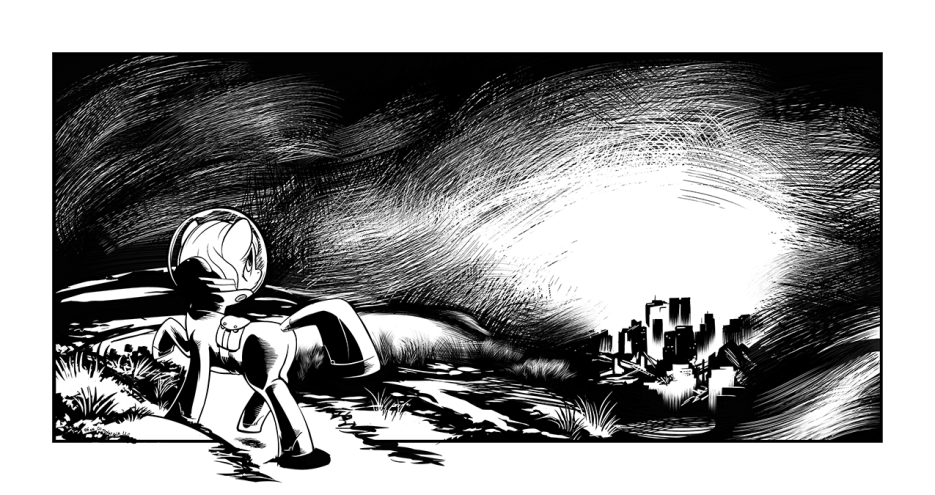
\includegraphics[width=0.9\linewidth]{image03.png}

\begin{intro}
Once upon a time, in the dying land of Equestria\dots
\end{intro}


\rtpr{``Good evening fillies and gentlecolts, this is Lonesome Pony speaking, and you're tuned to Radio 52. All the news you need to hear about Big 52 and nothing else! Well, almost nothing. In fact, it seems that now the biggest radio station in Equestria is broadcasting through all of the Wasteland. Some saint went down to Fillydelphia on behalf of DJ PON-3 and bucked the transmitter till it worked again. So hooray for those guys at Tenpony Tower, they took over the world!''}

Boisterous music played for a few seconds.

\rtpr{``Heh. That's everything from the big dogs, now back to the local news. Hey little ponies, are you afraid of ghosts? Maybe you should be. Do you remember the story of the Carnival? Don't worry if you don't. Good ol' L.P.'s going to give a quick recap for those that didn't do their homework.''}

\rtpr{``Far away on the north end of the Big 52 there lies a solitary barn. The Redtrotters call it `The Carnival.' It's a cursed relic from a long lost age, but unlike a lot of its siblings it never went to sleep. Once a year since before my grandpa could remember, a ghost would leave the building and lurk in the hills nearby, inviting everypony to its party and looking for company. When the next morning came, a foal was gone. No matter what, nopony ever returned. Approaching the Carnival was suicide thanks to the laser turrets that defended the place, but if you did succeed in getting close enough without being shot, you could hear music coming from the cursed barn, all day and all night long. A permanent party of horrors.''}

\rtpr{``Well, my little ponies, it seems that somepony just yelled 'I ain't afraid of no ghosts!', rushed inside the barn with the party in full swing and literally blew the roof off that whole place. No more foalnapping ghosts for the Redtrotters! I tried to gather some information about this benefactor, but what I got was a bit messy. Apparently, the one who did it some sort of ghost itself---a filly wearing a yellow radsuit and rising from death out of a pink cloud. Well, Yellow Ghost, nice work. One problem solved, nine-hundred-ninety-nine to go. Oh, and did I mention that this year's victim made it safely home? Celestia bless our souls! And now back to good old Pony Marcus!''}

\begin{music}
		I can see that lone star from a thousand miles away,
	
		Calling me back home, though I've ventured far away.
	
		When I see that beacon shining for me all along,
	
		It calls me to Equestria and a home!
\end{music}

\horizonline

\englishdaytimeplace{4}{00:30 A.M.}{Salt Cube Flats, Big 52 N Branch}

Puppy trotted along Route 52, heading south. The big city had grown from a silhouette on the horizon into a large, sprawling mass just a few kilometers in front of her. The foal had trotted all day long, and now the light was fading into darkness. Her eyes began to turn bright pink, shining in the night while she walked down the road. Without the daylight it was possible to see a green glow around the dome of Salt Cube City, while the bigger skyscrapers of Downtown were lit with sparse fires. The largest part of the city simply faded into the darkness of an ever-clouded night sky.

Around midnight, the filly in yellow spotted a small caravan heading in her direction from the south. There were about half a dozen ponies, and they had some sort strange two-headed cows with them. Puppy sat down in surprise, and waited for them to draw near. The caravan guards spotted the foal soon afterwards, being that she was a light source sitting by herself in the middle of the road. Needless to say, the guards were already on edge.

A large buck wearing a light combat saddle mumbled to another. ``What do you think, could it be that 'ghost' from the news?''

The leader of the guards, an earth pony mare with a big revolver, shrugged. Raising a hoof, she made the caravan stop. ``Dunno, but I'm not taking any chances. Let's move. Two on the sides, two here. I'm trying a diplomatic approach. Cover me or you can forget your pay.''

Two of the guards detached from the caravan and left the road, circling Puppysmiles, one on each side of her. Meanwhile, the leader ran ahead while the caravan with the remaining two guards kept their distance. The sight of the filly was quite an eerie one. The creepiness of the small yellow silhouette, which had a glowing pink light coming from its glassy helmet, was already a perfectly valid argument for opening fire. The leader of the guards approached the creature with caution, hoping that the other two guards were fast enough on the trigger in case of complications.

``Hi! I'm Puppysmiles!'' The foal raised a hoof, waving to the guard leader. Well, at least it didn't seem hostile.

In the Wasteland Survival Guide, there's a sentence that dwarfs all others when it comes to the sheer number of iterations: \emph{better safe than sorry.} Not seeming hostile didn't mean it was safe. ``Okay, now don't move, and tell me what you are and why I shouldn't transform you into fertilizer.''

Puppy giggled. Fancy words always made her giggle. ``Tee-hee, pretty pony is funny! I'm not Forty Liza, I'm Puppysmiles! What's your name?''

The guard leader hesitated for a moment. Was this foal simply retarded, or was it all part of some well-planned trap? The whole situation just smelled wrong. ``Yeah, I'm Solid Slug. Are you alone?'' Without waiting for an answer, the guard gestured to the two on her sides to check the surrounding area.

``Nopey mopey, I'm with Mister Voice! He's super smart or super stoopid, it depends. But for sure, he knows where my mom is!''

``And where is this `Mister Voice' now?''

``Inside the space suit! See all the lights and the pretty dots? He makes them appear!'' Okay, there was a nine out of ten chance that she was just a retard.

Solid Slug took a better look at the suit's helmet, trying to ignore Puppy's brightly shining eyes. There was an active HUD, quite similar to the one used in some models of battle saddles. Upon closer examination, the harness seemed like a very expensive piece of equipment. Solid wondered how a foal could ever find something like that, but the pink light emanating from the suit gave her the feeling that there was more to the situation. Solid Slug had been in the business for a whole lot longer than most caravan guards, and had picked up more than a thing or two about the Wasteland in all that time.

``Say, are you from Canterlot by any chance?''

``Yush! My house is, ah, was just under the mountain in Clover Leaf Terrace, but the other day it went down, so now I'm looking for my mom. She wasn't at the old barn, but Mister Voice says that there is another place in that big town so I'm going there now!'' Puppy pointed a hoof somewhere southward.

Solid Slug nodded a couple of times while listening, raised a hoof and gestured to the caravan. After some preparations the carts started moving again. ``Wow, you chat a lot, don't you? Lonesome Pony was speaking about your exploit at the Carnival.''

``My what? You mean the old barn? I didn't explode there, it was the barn that exploded, silly filly.'' Puppysmiles giggled. ``That Pinkbot was totally a baked bad! At first it was really creepy, but I'm a brave pony!''

Solid Slug scratched her head, trying futilely to follow Puppy's chattering. ``Uh, yeah, that's great. I'd stay here and chat for ages but we have to keep moving. If you're going to Salt Cube City, the ghoul community is at the Dome. I think they call it the Glow. Don't wander too much in Downtown, they don't like your kind. Oh, and, well, good luck, little ghost.'' When the caravan arrived the other ponies of the group sneaked curious looks at Puppy, but Solid Slug whispered to a purple unicorn with a red mane, and they simply kept moving. The filly in yellow stared with amazement at the brahmins and waved a hoof to the pretty ponies as they disappeared into the night. Once she was on her own again the foal trotted away, heading south along the Route.


\horizonline

\englishdaytimeplace{4}{11:30 A.M.}{Downtown, Salt Cube City}

The gate was a simple barricade built from sandbags and salvaged metal plates. On a wooden platform, a pony with metal barding operated a chaingun, while two other guards checked every pony that wanted to get into Salt Cube City. One last unicorn wearing an officer's uniform sat inside a small metal structure making notes in a register.

It was almost noon, but the traffic on the north end of downtown was as dead as the Wasteland. This time Puppysmiles was ready. She had that metal thing with the painted apple and showed it to the guards. One of the armored ponies approached her while the others kept their weapons ready.

``Let's see. Yes, this is a valid pass. Now, what's your name and business here?''

``I'm Puppysmiles! What's your name mister pretty pony?''

The guard raised the visor of his helmet, giving Puppy an annoyed look. ``Corporal Farsight. Now, what's your business in Salt Cube City, kid?''

``Oh, I know this one! I'm looking for my mom! She's somewhere in that direction!'' Puppy pointed her hoof toward a cluster of ruined buildings and the guard sighed.

``Very well, I guess that's enough. Just another question---why are you wearing a full environmental suit?''

``Oh, this one? I'm stuck inside it, but that's okay because Mister Voice lives in the space suit too and he's helping me with my mission.'' She lowered her voice, whispering to Farsight, ``He's not very good with that, but don't tell him. He's quite grumpy.''

The guard lowered his visor again and shrugged. ``As long as you're not going to blow a megaspell in Downtown, you can dress as you like. Welcome to Salt Cube City, kid.'' Puppy trotted beyond the roadblock, but Farsight called her back one last time. ``Oh, and don't go anywhere near the Dome. There are feral ghouls in the area, and it's heavily irradiated.''

``Okie dokie lokie! Bye bye mister guard Farsight!'' Puppy trotted merrily toward the big skyscrapers at the bottom of the boulevard, although the pink arrow pointed in a different direction.

Downtown was a typical trade hub along the Big 52. There were guards that kept ponies from killing each other and a couple dozen tents with signs of the different trading companies operating in the area, like the Water Herders or the Bullet Gallopers. There were even freelance traders and some trading posts from the nearest tribes. The open market was placed in the streets, but the real Downtown consisted of the four skyscrapers that still stood in the middle of the settlement. Salt Cube City had been the target of a single megaspell during the war, and the missile vector that should have delivered it malfunctioned. The warhead hit the Salt Cube Dome in the city periphery, piercing the roof and exploding at ground level. The massive structure of the Dome had shielded the surrounding area from the worst effects of the direct hit, but not from the fallout. During the successive two centuries, the most weathered buildings surrendered one by one to the ravages of time, but the four biggest and least-damaged skyscrapers survived and still stood in the middle of the city.

The four towers were the symbols of power in Salt Cube City. Two of them were each the main hub of a trading company, while the third was the headquarters of the Hired Hooves, a powerful mercenary company. The last building was the smallest one and housed the White Apples, the original tribe that inhabited the city. They were formally the real proprietors of the whole town and got a share of all the commerce going on in the place. The White Apples were also the main breeding ground for the Hired Hooves, mostly consisting of the families of ponies that worked for the mercenary company.

Puppy stood in front of a small tent marked with a red splash, the symbol of the Redtrotters. The shop sported a vast array of melee weapons and light armor on the shelves. A mare with an old cowboy hat was sitting on an ammunition box just in the middle of the exhibition.

``Hey, nice dress, little one. Say, are you from the north?'' The mare smiled at Puppy and lifted her hat with a hoof, revealing a horn on her forehead. The cutie mark on her flank depicted a basket ball.

``Hi! I'm Puppysmiles!'' She waved a hoof and trotted toward the mare. ``I'm from there.'' Puppy pointed at the street outside the tent.

``I'm Play Maker. I think that Lonesome Pony mentioned something about you last night.''

``Uhm, you mean the chatty pony on the music channel?'' Puppy scratched her helmet with a thoughtful expression. ``Last time he was speaking of the importance of drinking pure water.''

``No, no, I mean the news about the Yellow Ghost. Uh, maybe there's more than just one pony wearing a radsuit around. Anyhow, what do you need?''

Puppysmiles frowned. ``Why is everypony calling me a ghost?''

Play Maker smiled. ``So it's you after all, I knew it!'' The unicorn tapped her chin for a moment. ``Say, aren't you a bit too young to destroy a cursed barn? Actually, aren't you a bit too young to go around on your own? Are you a Crusader?''

``Nopey mopey. I'm looking for my mom, and I'm not alone! I have Mister Voice with me.''

``Your mom? Maybe I can help you: a lot of ponies visit Downtown every day. What's your mom's name? What's her cutie mark?''

Puppy smiled widely. ``Oh, her name is Rainy Days, she's purple and has an orange mane and her cutie mark is a cloud with raindrops! Have you seen her? Mister Voice says that she's somewhere in this place! That way!'' Puppy pointed her hoof again in the direction of some destroyed buildings.

Play Maker shook her head. ``I'm sorry, kid. Can't remember a pony with that palette or cutie mark, and the name doesn't ring a bell.'' She looked in the direction that Puppy was pointing and frowned. ``That way, you say? That can't be good. That's the radioactive area. The only standing building in that direction is the Dome, and trust me, you don't want to go anywhere near the Dome.''

``The Dome? What's that?''

``It's a place filled with feral ghouls and other horrors. It's highly radioactive, but maybe that's not a problem since you're wearing a radsuit. The real problem is the inhabitants: a small community of fanatical religious ghouls live there, but they're on the brink of madness. In fact, some of their 'siblings' went mad and attacked the caravans heading here. There's quite a situation now, and the White Apples are looking for a way to get rid of those rot-heads. They blast any ghoul that shows his face outside, but they can't go in and finish the job. The whole place is a deathtrap if you're not immune to radiation, so they reached a stalemate.''

Puppysmiles frowned. ``What's a ghoul?''

``You're kidding me! You don't know what a ghoul is?'' Play Maker stared at the blank expression on Puppy's face and sighed. ``No, you're not kidding.'' She shook her head. ``A ghoul is a pony that was poisoned by radiation a long time ago, when the megaspells hit. Instead of dying they were transformed into---I'm not sure what they are. The living dead? Maybe some sort of zombie? Anyhow, many of them went crazy because of that mutation and became feral ghouls---aggressive creatures that attack and try to eat everypony they see. Others retained their sanity and became immortal, but were disfigured by the mutation. Their manes fell out, their hides burned away, and their flesh began to blister and rot. Every ghoul looks like a decomposing corpse, but somehow they remain alive. The problem is that sooner or later every ghoul goes `boing' in the head and swaps their current diet for a meatier one.''

Puppy frowned. The unicorn could see fear and realization in her eyes. ``Miss Play Maker? Um, if my mom is really where Mister Voice says, will she be okay?''

``I---'' She lowered her hat, hiding her eyes from Puppy. ``I don't know, little ghost, but the Dome is a dangerous place. I hope you're not going there after what I told you.''

Puppy stood on her hooves with renewed determination in her eyes. ``I have to go! My mom could be there, and she could be in danger!''

Play Maker immediately realized that she'd never be able to talk her out of this suicide mission. ``You're not family, so I can't tell you what to do and what not to, but please listen to my advice. Go to that tower, the one with the big white apple on the sign. Tell the pony at the entrance that you want to enroll for a scout mission into the Dome. They'll give you some equipment and maybe a weapon. You have a radsuit, and they're so desperate that they'll accept anypony that they think could at least stand a chance.''

Puppy smiled. ``Okie dokie lokie! Hang on, Mom, I'm coming to rescue you!'' The foal galloped out of the tent and eagerly rushed to White Apple Tower.


\horizonline

\englishdaytimeplace{4}{2:00 P.M.}{Salt Cube Dome, Salt Cube City}

{\mten ``Warning. Mild radiation detected. Threat level: negligible.''}

The Dome was a humongous elliptical structure that had once served as an expo center where a large number of events could be hosted at the same time. A gigantic, globular roof once covered the building, but now it was almost completely destroyed, leaving only the external walls still adorned with columns and arches that made the structure vaguely resemble an oversized coliseum.

A boulevard headed right to the main entrance of the Dome, a monumental arch that led into a hall where the huge remains of a marble statue littered a floor that was once made of polished stone tiles. Now, it was mostly a carpet of rubble. Puppy stood in front of the archway, looking at the pink arrow on the compass.

``Okie dokie Mister Voice, what are we doing now exactly?''

{\mten ``Ministry of Morale hub reached. Primary objective attained.''}

``Yes, I know that we are here. I'm asking what's next. What are we supposed to do here?''

{\mten ``Secondary objective: investigate the ghouls and/or get rid of them. Warning. Mild radiation detected. Threat level: negligible.''}

``So, we find these ghouls, ask them where is Mom and then we try to make them go away?''

{\mten ``Affirmative. This is one possible approach.''}

``Great, I love having a plan. Let's do it.'' Puppy stepped into the hall and yelled, ``HEY, GHOULIE PONIES!'' It echoed several times into the large structure. She didn't seem to get any answer, so the filly in yellow trotted toward a large staircase at the bottom of the entrance hall.

{\mten ``Warning. Heavy radiation detected. Threat level: negligible.''}

``Hey, I think I've seen somepony moving behind that statue! Hey you, wait!'' Puppy galloped in the direction of a shadow that was hiding behind the pedestal of another broken marble monument. As the foal reached the hiding pony, she slowed to a trot and called out to him or her. ``Hi, I'm Puppysmiles! Have you seen my‒''

That pony! It was him---Count Horse Tile! He was right in front of her, even uglier than she could remember and somehow a lot creepier.

{\mten ``Warning. Hostile detected. Feral Ghoul. Distance: two meters. Threat level: low.'' The creature was looking at Puppy's face, drooling a yellowish goo from its mouth. It seemed oddly uncertain about its next move.}

Puppy stepped back, terrified by the macabre sight. ``W-why are you still coming after me? Leave me be! Go away!''

The creature growled and lowered its head, so Puppy turned on herself and galloped away as fast as she could.

Alas, it wasn't fast enough.

The feral creature jumped on her, foaming and biting, aiming for Puppy's head. The helmet was designed to endure punishment, so the first assault of the raging beast simply hurt Puppy's innocence. The sight and sound of a mouthful of rotting, jagged teeth scraping against her helmet was enough to paralyze her with fear.

``EEEEEEEEEEEK!'' Puppy reacted on pure instinct. She tried bucking the ghoul away, but it was a lot heavier than she was, and it pinned her on the ground with its weight. ``Rock! ROCK! NOW!'' She didn't stop screaming as she grabbed \emph{The Rock Of Destiny} with both hooves and started hitting the monster repeatedly. ``Stop moving! STOP MOVING NOW!''

A couple of minutes later, Puppy was still beating the brown slimy pulp that was once a pony's head. The scratches on her helmet and some minor bruises on the fabric were already gone thanks to the self-repair spells built into the suit. Slowly, the beating simmered down until it stopped completely. The ghoul was positively immobile and Puppy needed to catch her breath. It had been terrible, but at last the dark shadow of Count Horse Tile was gone! No more hiding or running away. The monster was stopped once and for all, his reign of terror extinguished! At last Puppy felt relieved, until she raised her eyes from the dead ghoul.

And finally noticed the three other ghouls that were looking at her with empty eyes and drooling mouths.

{\mten ``Warning. Three hostiles incoming. Nearest target: twelve meters.''}

``Hey, Mister Voice. What is a miss under---uh---static?''

{\mten ``Misunderstanding. The act of giving the wrong meaning to a word or sentence, creating confusion. The more you know!''}

Puppy nodded slowly while the three ghouls looked in her direction from the end of the hall. ``Good. What is exactly a Horse Tile Count?''

{\mten ``Hostile count. Number of enemies or ill-intentioned creatures in sensor range. Actual hostile count: three. Feral ghouls. Threat level: moderate.''}

Puppy sighed, threw \emph{The Rock Of Destiny} at the ghouls, and charged. The ghouls did the same thing from the other end of the hall.


\horizonline

\englishdaytimeplace{4}{2:30 P.M.}{Salt Cube Dome, Salt Cube City}

{\mten ``Warning. Several breaches in the containment suit. Warning. Littlehorn Agent detected. Warning. Compass malfunctioning. Warning. Inventory management spell temporary offline. Warning. Energy crystal cells damaged. Emergency cells on 29.06\%. Warning. Deadly radiation level detected. Threat level: negligible. Subject deceased, condition stable. All clear.''}

Puppy stood in the middle of a scene of mayhem, decorated with goo and rotten flesh. The bodies of three ghouls lay scattered on the ground with their heads missing. The whole fight had taken a while and been very messy, since the ghouls kept regenerating because of the radiation in the area. However, Puppy had also been regenerating because of the Pink Agent and her radsuit's enchantments. In the end, the foal's dedication at aiming only for their heads won out over the brainless biting and bucking of the ghoul trio, but in the process she had been beaten like a bucking bag. Her flanks had been half eaten and a thin pink cloud invaded the area.

``Hey, Mister Voice? Are you sure that Mom is in this place?''

{\mten ``Affirmative. Actual position: Ministry of Morale structure ID 00201--Salt Cube Dome.''}

``Okie\dots dokie\dots lokie\dots'' Puppy stopped listening at affirmative and fell to the ground, exhausted from the fight. ``Because the only thing I want to do now is cry.''

A couple of figures appeared from another entrance of the hall. They seemed to whisper to each other before one of them took a hunting rifle while the other moved cautiously toward the filly in yellow. Puppy reached out with her hoof for \emph{The Rock of Destiny} in front of her and grabbed it, but her eyes were so tired. She just wanted to lie down a little more. ``Please, go away. Please,'' she whimpered, ``stop being mean. I'll behave.''

The nearest pony now was close enough to let Puppy take a good look at it. It was another ghoul, but somehow different from the others. This one was wearing a uniform similar to the one of the mare that gave her the suit. Moreover, it didn't drool, had some intelligence in its eyes, and last but not least, it spoke.

``Hey, are you okay little one? This place is very dangerous.'' The pony sounded like chalk screeching on a blackboard, but somehow Puppy felt like it was a mare's voice. ``Hey, Soft Air! We have to take this foal out from the radioactive zone before she dies! Do we have any Rad-X or some RadAway?''

``I don't think so. Stay out from the pink cloud, it seems awfully familiar. I'm almost positive it's dangerous.''

The scouting pony abruptly stopped before getting too near to Puppy and tilted her head. ``Oh, so it's not just my bad eye?'' The ghoul trotted around the pink cloud that was quickly dissipating, as if the suit were drawing it back inside itself in the process of self repairing.

{\mten ``Containment restored. Warning. Critical level of radiation detected. Threat level: negligible.''}

Puppy slowly rose to her hooves while the ghoul mare drew near and the other kept his weapon ready. The filly had to try something diplomatic. ``I, uh, hope that those ugly ponies weren't your friends?''

``The word you're looking for is ghouls, little one. And yes, there was a time when they were our friends, but I guess that right now you did them a favor. So, no bad blood.'' The ghoul mare stopped in front of Puppysmiles and took a look inside her helmet. The face of the filly was annoyingly well conserved, not showing scars or signs of deterioration, but the pink flames in her eyes, burning bright with the radiation of the place, spoke volumes about her nature. ``You are quite a strange ghoul. I'm Peach Blossom, what's your name?''

``Uhm, oh, yeah, I'm Puppysmiles. I'm looking for my mom, she's supposed to be somewhere in this place but all I found were these ugly ponies.''

Peach waved a hoof, calling her companion. ``Soft Air, stop being paranoid and come here!'' She went back to speaking with the foal in yellow. ``Could you please stop calling us ugly and just say ghouls? Anyhow, if your mother is here she has to be a ghoul too, otherwise she is going to be super slim. What's your mother's name?''

``I know this one! Her name is Rainy Days and she's super cool! Have you seen her?''

The buck coming near overheard the conversation. ``Rainy Days, Rainy Days\dots That name sounds familiar. If you give me a second or two to think about it I might remember something.''

Puppy looked amazedly at Soft Air. ``Really? Please please please where is she?''

``Hey, wait, I told you I can't remember her very well! My memory is not as good as it used to be. Anyhow, if you don't want to meet other ferals we should move. Let's go to the Glow.''

Peach Blossom nodded. ``Yes, let's get back, after all we found what we were looking for. Anyhow, Puppy, where are you from?''

``Canterlot!'' Puppy smiled with pride. Canterlot was the best city ever, why not be proud of it?

Both ghouls frowned, Peach looked away while Soft Air sighed. ``Oh, so you are one of those.'' Peach muttered to herself. ``War sucks.''


\horizonline

\englishdaytimeplace{4}{3:00 P.M.}{The Glow, Salt Cube City}

The Glow was mostly a small circle of tents pitched in the central hall of the Dome. The roof was missing and large metallic debris littered the ground. The tents were all sporting a symbol of three pink butterflies on a yellow background, and were large and sturdy, being made of a tough material that was built to last. They had survived for more than two centuries.

Quite obviously the Glow wasn't called as such because of the tents, nor for the ghouls. It was the twelve meter tall salt cube glowing in a blueish-green light that earned the Glow its name.

{\mten ``Warning. Radiation level off the scale. Sensor emergency shutdown activated in order to prevent irreversible damage. Threat level: negligible.'' The HUD of the helmet disappeared. Puppy frowned for a single moment, then shrugged. Maybe even Mister Voice needed a little sleep sometimes.}

The cube was drawing all of Puppy's attention at the moment. It was shiny and glassy and super nice. The foal wondered if she could have some little shining cubes to keep in her bedroom. This could get rid of that bad scary monster that lived under her bed. For a moment she missed her home and felt like crying, but she was a filly on a mission, and she didn't have time for these things, so instead she asked, ``What's that pretty shiny cube? Can I have a shiny cube too? Please? Puppy please?''

Soft Air chuckled. ``I don't think so, Puppy, but I could have something nice for you if you will be a good pony. Deal?''

Puppy started jumping all around. ``A present? For me? Gimme gimme gimme!''

``Now, now, I told you to behave, right? First of all we are going to have a little chat with Sand Box, then we'll try to find out about Mrs.~Rainy Days.''

Puppy stopped jumping and began to trot alongside Soft Air and Peach Blossom. ``You know? Even if you're pretty ugly you are funny and nice ponies.''

Peach deadpanned. ``Well, thank you, miss monster. Anyhow, there he is, Sand Box, the leader of the camp.'' Another ghoul was looking at a block of paper, reading it and scratching his head seemingly in confusion. ``Even if he seems elsewhere at times, he's smarter than the average scientist. Hey, boss, we got a visitor.''

The leader of the ghouls was wearing an old lab coat and a pair of glasses, and seemed quite alarmed from the look he was giving the papers in front of him. The ghoul replied without even looking at Puppy. ``Yes, great, give him the usual speech and warn him against Downtown. Excuse me, but I'm trying to avoid a cascade.''

Puppysmiles giggled and trotted up to him, trying to look at his face. ``Tee-hee, ugly pony says fancy words! Hi, I'm Puppysmiles, but you can call me Puppy! Have you seen my mom?''

Peach tried to stop the foal but it was already too late. She opened her mouth to speak, but was interrupted by the reaction of her leader. Sand Box adjusted his glasses and studied Puppysmiles for a moment. ``Luna buck me if I thought I'd see another functioning Mark VI. That was a hay of a failure, wasn't it?''

Both Peach and Air tilted their heads, staring in puzzlement at Sand Box as he continued. ``They were designed to keep foals safe from the worst effects of a fallout, loaded with all the best medical talismans and up-to-date logical spells that in some cases were even more advanced than the ones used by Stable-Tec in its PipBucks.'' He shook his head, his expression turning sad. ``What we didn't expect was the reaction of all this technology and magic in case of a Pink Agent attack. The suits had enough medical supplies and healing power in their talismans to mitigate the first effects of the gas, creating the perfect conditions for a uh, merging process.'' The scientist turned toward the other two ghouls. ``Have you ever heard of the Ghost Herd?'' Both ponies shook their heads. Sand Box put a hoof around Puppy's neck, making her stand next to him.

``It was about a month past the day the Goddesses fell. A small herd of little ponies wearing yellow suits, just like this one, left Canterlot. Most of them lost their minds because of the mutation, the others had simply no clue about what was going on. They were ghosts indeed\dots Obsessed with the loss of their parents, and clueless about what happened, they wandered together mostly because everypony else in those days was dead. The herd came here, heading south. They met some survivors on their path, but the crazed ones simply slaughtered any living thing that they met. The others, well, they were afraid of being alone and followed the herd.''

Peach stepped back. ``She doesn't seem that dangerous to me.''

Sand Box chuckled and kept narrating his tale. ``They are mostly immortal like us ghouls, but they rise from their own dust unless you tear their bodies apart, like Canterlot ghouls. Even worse, the MK VI has a very advanced self-repairing spell that lets them recover even from some amputations and such. They are quite the little yellow devils.''

Soft Air tapped his chin. ``But if they were so invincible, where are they now?''

``I have no idea. Most of them were taken down, at last. A decapitation combined with the destruction of the main spell matrix and the backup system should do the trick, but it's not that easy if you don't know what you're doing. Anyhow, at some point they left, disappeared and were never heard from again. The whole thing lasted a couple of months at most. You had to be there to remember them, but it was quite a disheartening sight. All those foals left alone and cursed in a dying world. Poor things.''

Sand Box patted Puppy on her helmet. She listened to the whole story trying to follow it, but she seemed a bit confused. ``I don't like this story, it makes me sad.'' Sand Box simply sighed and kept his hoof around Puppy's neck.

``Don't worry, little one. It's just an old ghost story, don't let old mare tales sap your enthusiasm. I think I have a Pinkie Pie plushie somewhere. Let's do this: just tell me why you are here and I'll give it to you, yes?''

A large grin appeared on Puppy's face, the boring story of the ghost herd already forgotten in favor of a way more interesting new toy. ``Sure! I'm looking for my mom! Her name is Rainy Days, and she is the best pony ever!'' Puppy seemed to remember something else. ``Oh, right! And I'm here to tell the ghouls to go away and never come back! Have you seen any ghouls around, Mister Ugly Pony Boss?''

Peach Blossom facehoofed.

\clearpage

~\vfill

\begin{engnote}
	Level up! (2)
	
	New perk added: Little Leaguer - You gain a +5\% in throwing, melee and unarmed combat.
\end{engnote}




\chapter{Vola Mio Mini Pony}

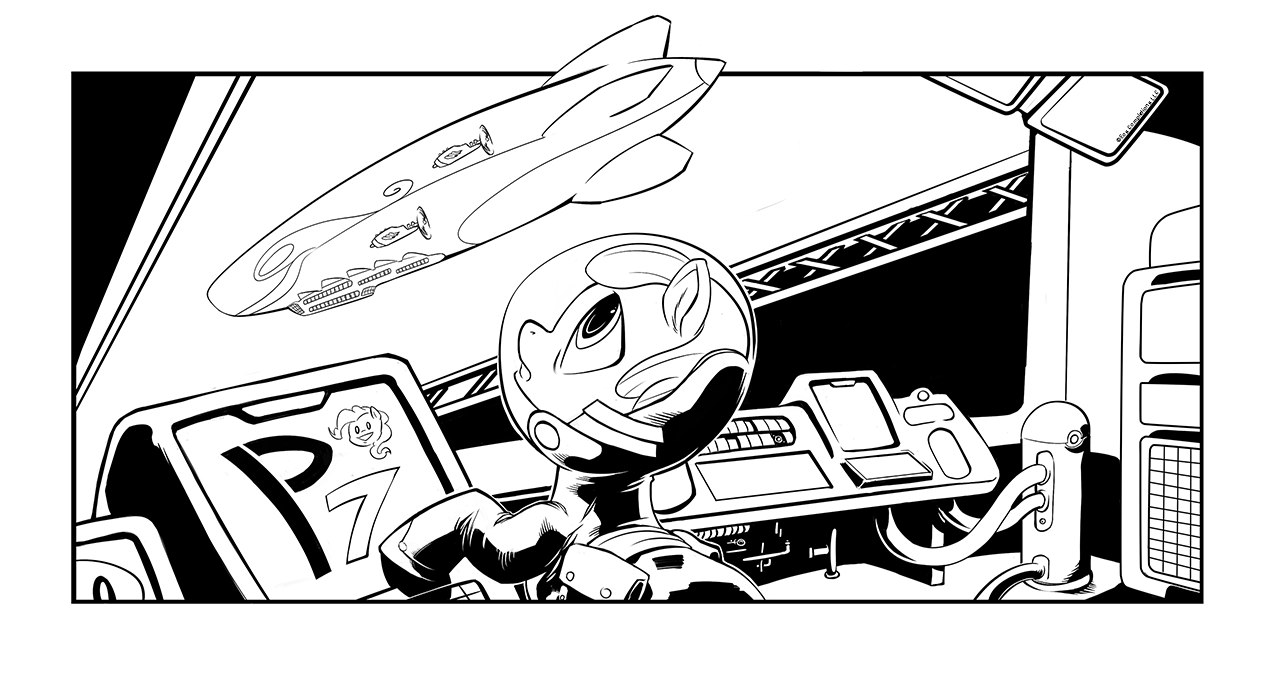
\includegraphics[width=0.9\linewidth]{image04.png}

\begin{intro}
Do you know you're all my very best friends?
\end{intro}


\englishdaytimeplace{4}{3:15 P.M.}{The Glow, Salt Cube City}

``That's impossible, ghouls are super stoopid zombies that eat ponies! You are ugly but mighty fine ponies, so you can't be ghouls! If you're not telling me where the ghouls are I'm going to look for them on my own! BLEH!'' Puppysmiles stuck out her tongue.

Soft Air and Peach Blossom exchanged a rapid glance, then Peach spoke, ``We have no reason to lie to you, Puppy. We are ghouls, but not every ghoul is a mindless pony eater.''

``But they told me‒''

``But you listen only to what you want to hear! Gee, you are a pain in the flank, did anypony ever tell you that?'' Peach sighed in relief, glad to have finally let that off her chest. It wasn't nice, but Puppy seemed more than simply spoiled. She was completely selective about any information she received. ``Wake up, ghost! This is not some\dots some magical land! This is Equestria, the worst sinkhole ever!''

Puppy stepped back, scared either by the decomposing pony that was scolding her, or by the profound truth in her words. ``B-b-but‒''

Peach stomped a hoof on the ground. ``Stop playing the innocent foal! You're a monster like us! Stop pretending! Now!''

Puppy backpedaled, falling on her haunches and trying to hide her face with her hooves. ``Please! Please stop! I'll behave!''

``I don't want you to behave! I want you to \emph{wake up}\/!'' Peach stomped a hoof on the ground.

Soft Air put a hoof on Peach's shoulder. ``Please calm down. I don't think she's pretending; don't let your anger drive you.''

She shoved away Air's hoof. ``She's two hundred years old, how can she be this naive? Is she a retard? I think she's just playing with us, and I think that we should‒''

Peach was interrupted by a long, eerie wail. For a moment, her mind rushed back to her foalhood, to that very day when she locked herself in the cellar by mistake and nopony came looking for her until night had fallen. She recalled the fear of being forgotten, the loneliness, every single creak from the barrels. Peach almost lost her voice calling for help, but it was the fair day. Nopony heard her. With an overwhelming sense of guilt, she realised that Puppy wasn't playing with them.

All the ghouls turned their attention to Puppy, as her long howl echoed something supernatural. It was the stuff of nightmares made audible, and struck hard on everypony in the camp. Maybe this happened because they were used to seeing a ghoul's rage, but this was the first time in decades that they had heard a foal's cry. Sand Box hesitated for a moment before walking to Puppy and hugging her.

``What, what the hell is she doing? That sound\dots'' Peach staggered, trying to stand on her hooves.

``I think that you made her cry,'' Soft Air answered flatly. ``Well, now I guess that it will be easier to make her accept the fact that we are the bad guys, right? Mission accomplished.''

``Oh for pete's sake, can you make her stop?'' complained a ghoul wearing an orange helmet on his head. ``I can't hear my thoughts!''

Sand Box continued to hold the foal as her sobs gradually lessened, growing quieter and quieter until they could barely hear her whispering half-spoken apologies. ``Now, now, I'm sure you are a good pony. You just miss your mom and that is okay.'' He rubbed Puppy's shoulders. ``Everypony has a bad day here and there. Peach Blossom was quite upset, but now you will say that you're sorry and she will forgive you. Just please, pay attention to her when she is explaining anything important, okay?''

Puppy nodded slowly and tried to establish eye contact with Sand Box, finding some relief in his elderly eyes. She turned to the ghoul mare and lowered her head. ``I-I'm sorry I didn't believe you, Missus Peach Blossom. I know that you are a ghoul now, and I was wrong.''

This made Peach feel even more guilty, but she had to play along. At least this way the conversation was going somewhere. ``Oh, it's all right little one. Just pay some more attention when the older ponies try to teach you something.'' She paused, thinking. \emph{What now?}\/ ``Uh, I think I remember you saying you want us to go away from this place? Why?''

Did I already say that Puppy was easily distracted?

Puppy scratched her helmet while thinking about this brand new question, but she couldn't seem to find a proper answer. ``I think\dots it was because those pretty ponies promised me a piggyback ride on a two-headed cow if I came here, took a look around, and go back and tell. They were also speaking of how great it would be if the ghouls were totally gone.'' Puppysmiles paused for a moment, trying to remember the rest of the story. ``Oh, right, so I said that I was going to deal with the meanie ghouls but they told me no. I replied that I was big enough to shoo a ghoul away whatever it was and they made me promise to just come here and take a look, but I crossed my hooves so that promise doesn't count.'' She smiled widely, clearly proud of herself. ``I was smarter than them!''

Soft Air snickered. ``Oh sweet Celestia, this filly is hilarious. Can we keep her?''

Sand Box sighed. ``This is a strange coincidence. Peach, please go and find Dr. Get Well. I need to speak with her quite urgently. Soft Air, can you keep an eye on this little prodigy for a while? Go to my office and grab that pink toy for our little guest.''


\horizonline

\englishdaytimeplace{4}{4:00 P.M.}{The Glow, Salt Cube City}

Puppy loved her new Pinkie Pie plushie. When she wasn't hugging it tightly, she was showing it to everypony she met. Too bad that it was mostly just Soft Air. ``See? She is super cool, way better than that killing Pinkbot! I bet she's super soft!'' She poked the plush with a hoof. ``Aw, stoopid space suit! I want to kiss her but I can't! I'm calling her Silky Tail!''

Soft Air knocked on Puppy's helmet. ``Hey space pony, look at what I got here.'' He pulled out a holotape for Puppy to see. ``Guess what this is?''

Puppy tilted her head. ``Uh, a black thing? I know I know! It's some stuff that does other stuff!''

``Wow, I couldn't explain it better. Okay, little miss scholar, come here and let me connect it to your suit.'' He took Puppy's left hoof and opened a small socket on her wrist, then slipped the tape inside.

{\mt ``Backup copy initiated. Reading. Warning. System working in emergency mode. Reproduction is impossible. Backup copy finished. The file will be opened as soon as the system begins running on normal mode.''}

``Hi Mister Voice!'' Puppy waited for a moment but she got no answer. ``See what I mean? I don't even know what I did to him but he's been keeping a grudge since we arrived here.''

``Oh, don't worry, it's just the salt cube. It interferes with smaller talismans and their circuitry.'' Soft Air watched the smiling foal for a moment. She was totally listening to everything and probably understanding nothing. Soft Air sighed. ``It makes Mister Voice sleepy. He'll wake up when you two leave the Glow.''

Puppy nodded. ``Don't tell this to anypony, but I feel a little lonely sometimes. I don't mean that I have no friends, but in the last few days I walked a lot and everypony had other things to do and nopony really wanted to stay with me, so\dots'' Puppy lowered her eyes. ``Mister Voice is a bit stoopid and he uses fancy words and he's grumpy, but he never leaves me. I hope he's not angry.''

Soft Air was going to say something, but he was interrupted by the sound of two ponies arguing with each other. ``We don't have that much time! The cascade is accelerating, can't you see it yourself? It's turning cyan already!'' he heard Sand Box say through the door.

``I'm not blind, and I'm beginning to think that you're going crazy! We need at least a couple days, it's not just\dots open the roof, inflate the balloons, and goodbye impending doom! I need time to initialize the system, reprogram the autopilot, and lay the course. Two days, maybe thirty hours, with no sleeping at all,'' came a mare's voice.

``It will release in seven or eight hours at best as soon as we start moving it, and if we wait that long it could be too late to even try anything.''

``Now I wonder why this came out all of a sudden. That damn cube was here even before the Dome was built, and you give me a seven hours warning before apocalypse?''

Puppy turned her head toward the voices. ``What's going on?''

``I have no idea, little one.'' Soft Air frowned. This was bad news, but there was no point in explaining the situation to Puppy. Odds were that she wouldn't even understand it and, if she did, it would only make her panic. ``Hey, do you want to see the gift shop in the northern hall?''


\horizonline

\englishdaytimeplace{4}{4:45 P.M.}{The Glow, Salt Cube City}

``\dots And that's how Equestria was made,'' concluded Puppy.

``Ah, yeah, that was an amazing story, but I asked you who this `Questioner' pony was that you were talking about.''

``Oh, that story! Nah, it's boring. What about that time that I ate a butterfly?''

Soft Air lowered his head, sighed, and muttered, ``I was running down the street when I saw a super duper mighty pretty---''

At the same time Puppy started talking while jumping all around. ``I was running down the street when I saw a super duper mighty pretty---''


\horizonline

\englishdaytimeplace{4}{5:15 P.M.}{The Glow, Salt Cube City}

Sand Box poked his head inside the gift shop. He immediately spotted Puppy and Soft Air and sighed in relief. ``Oh, here you are. You shouldn't wander this far from the Glow, there could be ferals in the area.''

Soft Air chuckled. ``Oh, don't fret about that. Little miss miracle here solved that problem.''

Sand Box tilted his head. ``You mean she was attacked by feral ghouls?''

``Eeyup. Four at once, it seems. I'd say that this little filly can fend for herself.''

``I hope so,'' sighed Sand Box, ``because I desperately need her help.''

``Hi Mister Ugly Pony Boss!'' Puppy jumped in front of him, sporting a broad smile. ``I like this place! I had a great idea! I can say to the ponies of the other town that all the ghoulies are gone so they will never ever bother you! Then we find some nice dresses and you'll disguise yourselves as, uhm, something not ugly and change your names, like Madame Le Flour and such! Isn't that a great idea? Oh, yeah, and we'll need a trombone!''

Sand Box cocked his head, then a sad smile spread across his decomposing face. ``Oh, I'd love to try that one, really, but I came here to inform you that we are going away. We're leaving the Glow.''

Puppy's ears flattened. ``You're going \emph{away}\/? B-b-but you can't go away! This is your home, you are not meanies, why are you going away?'' She was already hyperventilating. ``Wait a moment, I have another idea! We can try to give the other ponies a super nice present and throw them a party so they'll know that you're not evil! It could work, it must work!''

Sand Box sighed and put a hoof on Puppy's helmet. ``Don't fret your pretty head, my little pony. This is not your fault. It's just something that needs to be done, and I'm going to need your help to make it happen.''

``Sand Box, could you please explain to me what's going on? I overheard you and Get Well talking about the FFO. Has this anything to do with that cascade you were mumbling about when we arrived?''

Sand Box adjusted his glasses. ``Indeed. We already knew that the cube was not stable. Over the years it has absorbed and released the radiation from the megaspell in a cyclic pattern. As I already explained, in the last few months this cycle has accelerated. I think that the cube has reached the point of no return, and in less than five hours it's going to release.''

Soft Air's expression darkened. ``Well, that does not exactly leave us a lot of time. So, what now? I reckon that the Friend Force One still needs more than a little work. Are you sure about this release thing? Do you have any idea what will be released?'' She already knew the answer, but she still had the hope of being wrong.

``I'm not sure about that. It could either be the biggest mag pulse ever, or the original balefire that was embedded into the zebra's warhead. When the missile hit the Dome the cube absorbed the matrix of the spell. The problem is that we are speaking of a huge chunk of pure salt that wasn't designed for some anti-megaspell defense. Its behavior is highly unpredictable at best, a death sentence for Salt Cube City at worst.''

Puppy tried to follow the discussion, but it was too technical for her. They used all sorts of fancy words mixed up with other terms that she wasn't even sure were real words, so she decided to go and sightsee some other places of the Dome by herself.

Soft Air put a hoof on Puppy's helmet, pinning her in place before she got away. ``The FFO navigation system still needs calibration, and the autopilot is not working.''

``True, but I won't be depending on those systems. I'm going to fly the airship myself.''

Soft Air's mouth hung open in shock. ``Are you kidding me? That's suicide! Moreover, you can't fly that behemoth on your own, it requires at least somepony in the engine section, and a lot of work around the hydrogen tanks.'' Soft Air looked for a moment at Puppy, then a shadow of fear appeared on his face. ``Are, are you going to ask her to---''

``No, don't worry, she's just my ticket out of here. The artificial intelligence talismans of the MK VI suits were a sub-product of the P7 project. She'll be able to operate the control room just by stepping inside it, which will buy us time.'' Sand Box hesitated. ``Did you really think that I could take her with me?''

``Listen, we could simply evacuate the area and let the Cube blow those bastards in Apple Tower to kingdom come. We don't owe them anything, and they even shoot us on sight if we try to leave the Dome. Let's hit the tunnels and let them taste this muffin.''

Sand Box looked straight into Soft Air's eyes. ``You can do whatever you want. I'm asking Puppy to open the roof and give me clearance for the take off. I don't know how far I'll get, but I refuse to be responsible for the death of another single foal. In those towers there aren't just the ponies you hate, Air. You are forgetting the foaling mares and the young ones. Do they deserve your hate too?''

Puppy was still trying to move, pushing with her helmeted head stubbornly but without avail against Soft's hoof. ``Lemme go! I wanna play outside!''

Soft Air looked at Puppy. She was so naive, she wasn't even aware of the horror she was already living. Even telling her to run away as far as possible would have been useless. She was freedom itself, and if a megaspell was really going to detonate\dots ``I can work the engines, just tell me what to do.''

Sand Box nodded. ``I knew I could count on you. Peach is coming too, and Dr. Get Well is already aboard working on the commands. The others are preparing the cube for transportation. Now I need to teach Puppy her part, so this may take a while.'' He looked at Puppy. ``Hey, little one, want to explore a new place?''


\horizonline

\englishdaytimeplace{4}{6:30 P.M.}{The Glow, Salt Cube City}

\rcpr{``One more time, sunshine.''}

\rcpr{``But Mommy, I repeated it one gazillion times!''}

\rcpr{``Just one more time, okay? This is a super special secret magic spell. You have to say it without mistakes or it will not work. One more time for Mommy, please?''}

\rcpr{``Uh, can I have muffins then?''}

\rcpr{``It's almost lunch time, but you can have muffins if you'll eat all the alfalfa.''}

\rcpr{``That's not fair! You always give me too much of it!''}

\rcpr{``And you'll even get a super double hug.''}

\rcpr{``Uh, okie dokie. When I'm in front of the large round door I have to put the hoof on the green button.''}

\rcpr{``Very good.''}

\rcpr{``Then the genie will ask me the eye dentification cow. And I must say. Uh, a hint, Mommy?''}

\rcpr{``Oh, I know you remember it. Just wait a moment and think again. Mommy knows that you are a smart pretty pony.''}

{\mt ``Please state your identification code.''}

\rcpr{``Uh\dots FT\dots 0\dots 0\dots 1\dots 6\dots 5\dots RD\dots C\dots 1\dots G\dots A''}

\rcpr{``Right! See? It's easy! I knew you could do it, Puppy . And then what happens?''}

\rcpr{``Uh, the genie asks the other word, the pass code.''}

{\mt ``Please, state your pass code for this ID.''}

\rcpr{``Yes, and you must say\dots''}

``Hi, I'm Puppysmiles!''

{\mt ``ID accepted. First class field technician Rainy Days. Access to the control room granted. Warning. There are three thousand, six hundred ninety-eight error messages to process.''}

\rcpr{``And remember, if you hear the loud honks you must run to the secret place I told you and use the magic words. Don't wait for me, understood?''}

\rcpr{``Sure, Mom!''}

\rcpr{``I love you Puppy, now come here and get your hug.''}

This wasn't exactly the place where Mommy told Puppy to run, but the other day when there were the honks she didn't want to go underground when everypony else was playing outside. Oh well, this door asked for the magic words and they worked! Maybe this was a double super special secret magic spell? Go figure.

Behind the doors there was a large room with blinking panels. The far wall was actually a clear sheet of glass, covered in a spiderweb of cracks, and the whole room was illuminated by a couple of flickering lights in the ceiling. When Puppy stepped into the control room the door closed behind her.

{\mt ``Warning. Mild radiation detected. Threat level: negligible. Activating all systems.''}

``Mister Voice you are back! It was about time.''

{\mt ``All systems are working properly. Detected attempt of opening a communication bridge. Checking source. Source confirmed: Ministry of Morale structure ID 00201---Salt Cube Dome Control Room. Comparing protocol. Warning. This suit system version is outdated. Updating: please wait.''}

``Wow, you sure chat a lot. Did you miss me? I missed you a lot! I found those ghoulie ponies we were looking for, but they weren't evil! Instead, they were nice, just a bit ugly. And Peach scolded me, but I was a bit meanie with them so I said I was sorry and then it was all right! Then Mister Soft Air gave me a-''

A sudden ringing noise interrupted Puppy. She stood there confused for a moment before launching herself in search of whatever had made that funny noise. After some jumping and skipping, she found a red telephone just in front of a dusty desk. Puppy picked up the receiver, ``Hallo? Mom's not here and I'm too little so I can't take a note. Can you call at dinner, pretty please?'' The universe d'awwed.

``Puppy, it's me, Sand Box.'' A familiar voice hummed from the phone. ``It seems that my hacking device worked, as you're now inside of the control room. We still need some time to replenish the battery boxes and pump out the hydrogen. So for now, it's very important that you stay inside that room.''

Puppy looked for a moment at the weird transmitter that Sand Box had given her before they parted. ``Oh right, the thingy! I didn't use that, I forgot!''

``But how did you\dots doesn't matter, now please listen carefully to me. I'm going to hang up the phone, but I'll call you back when we are ready. Wait there and don't touch anything until I call back, okay?''

``Okie dokie lokie! Bye bye!'' Puppy put down the receiver and started looking around. The whole place was dusty and grey, quite a sad room that reminded Puppy of that stoopid place with the humongous round door, only this one was little and with a lot of desks and screens, mostly broken.

Suddenly a line of red lights appeared on the big desk in front of the damaged window. Immediately afterwards, more red bulbs came to life, this time on almost every desk. Several screens began to flicker with a green light. Puppy sat on her rump, a bit disoriented. ``Hey, I didn't touch anything! Cross my heart!''

{\mt ``Update complete. P7 lite client version properly installed. Rebooting system.''}

The whole suit went dark and Puppy again felt that sensation of immobility just like the day she awoke in Canterlot, but this time it lasted for less than a couple seconds.

``Uh, I feel funny.''

In front of Puppy's face the HUD of the helmet flashed with a pink light that occupied her whole vision. In the middle of the pink square there was seven balloons tied together, then the logo disappeared, leaving the usual interface with the compass on top and the other useless things down left and right. What really surprised Puppy was the voice that came with all of it---not Mister Voice, but a different one---a feminine tone that was quite high pitched and very friendly.

``Hi there, Miss Days! We have a little bit of a situation here. All the screens are gone for good, and we are missing, uh, 100\% of the personnel. They haven't been to work for about, woah, that's a lot of time! The bigwigs should seriously consider a little turnover here! Oh, but don't worry! I can operate everything just fine from your personal console!''

``Who are you? Where's Mister Voice?''

``I'm Pinkie Seven! Your best friendly pony-machine interface! I'm programmed to not try to take over the world, nor become a judging god machine! I'm pretty nice, aren't I?''

Puppy scratched her helmet for a moment. ``Do you know Miss Pinkbot?''

``Why yes! Our top of the line entertaining prototype! It's being tested at, no wait, the test ended a couple days ago, let's see the results. Well, it seems that the party was so great that it made you simply die! No wait, it's intended literally. That doesn't sound that good! Well, let's never speak again of the Pinkbot project, okie dokie?''

``But it hurt a lot of pretty ponies.''

``Data deleted. I'm sorry, I don't know what you are talking about. Now, what was the other thing?''

``Uh, the Pinkbot?'' tried Puppy.

``Never heard of it. Anything else?''

``Ah, yeah, something about a flying thingy.'' Puppy tapped her helmet trying to remember. ``Where is Mister Voice? I think I like him better.''

``You, you don't like me? You don't want to be my friend? But why, I'm trying so hard! I waited here for, like, two hundred years! Please don't send me back to the mainframe! It's dark and lonely and I can only count the machine cycles down there! PLEEEEASE!''

``Uh, if you're sure you're not going to foalnap somepony.''

``No way, there must be a rule against that in my program, don't worry. No foalnapping, no mass extermination, no moral judgment. Just your average little helping pony routine, don't worry! And, say, I know this is not going to help our relationship, but the security protocol is annoying me with a little detail.''

Puppy giggled. ``Tee-hee, Miss Voice uses fancy words!''

``Yes, sometimes I do that. Say, are you first class field technician Rainy Days? Because your console here says that your name is Puppysmiles.''

``Silly Voice! I'm Puppysmiles!''

``Oh great, just what I needed, a breach. Two centuries in a dusty talisman and the first time I can have some fun it's an intruder.'' Miss Voice paused for a moment. ``Miss Puppysmiles, your presence is not authorized. I must ask you to leave. You have no idea of how much this hurts me.''

``B-but Mister Sand Box said that I must be here or the friend ship will not fly! Can I stay just a little more? Pretty please? Puppy please?''

``If you want to stay you need an authorization from the chief of the staff or from a military officer with at least the rank of colonel. I really, really, REALLY want you to stay, but my hooves are tied! If I only had something to work with, like, I don't know, a logical paradox or some funny program loop. Oh, wait. What's your relation with the head technician?''

``Who?''

``Rainy Days.''

``Oh, she's my mom! Do you know where she is?''

``Oh, this fixes everything! Let's see, yes, I can move this here and that there and then voila! Today it's bring your daughter to work day! Are you happy?''

``Uh, I still want my mom.''

``Hey, look at this, it's even in your mission logbook! You are really fond of your mom aren't you?''

``Well, duh, she's my mom!'' Puppysmiles exclaimed.

``Listen here! We can make a‒ oh wait, call incoming on the emergency line.''

The voice of Sand Box replaced the one of the artificial intelligence. ``Hey, Puppy, we're done here. Are you ready?''

``Hi, Mister Boss! Sure I am, and this Miss Voice chats a lot!''

``Great, now listen carefully. There are a couple of ponies that want to say goodbye. Please behave and do not take too much time because we're running a bit late.''

The voice of Sand Box was replaced by Peach Blossom. ``Hey, little one, are you there?''

``Hi, Miss Peach!''

``Good, I'm so happy to hear you. I wanted to say that I'm sorry, I didn't have to scold you. Peace?''

``Uh, okie dokie?''

She sighed in relief. ``Thank Celestia, I couldn't do this with that weight on me. Please remember this Puppy: Equestria is an unforgiving place. You have to treasure your friends because they will be very few. I\dots I regret that we didn't have time to get to know each other better, but I know that you are going to be safe, so I have no regrets.''

``Are you going away? I can come and visit you when you get there, okay? We will trow a party!''

Peach stopped, taking some time before speaking again. ``Yes. Yes Puppy, if we meet again one day, we will `trow' a super party\dots Sorry, I have to go.''

The phone went mute for a moment before another voice started talking. ``Hey Puppy, Soft Air here. Please follow Sand's instructions very well, we're all counting on you here!''

``Hi, Soft! Mister Voice now is Miss Voice! Isn't that funny?''

``What are you talking about? Aw, it doesn't matter, I have to tell you something. I knew your mother. Now, please don't panic. I have little time and you really need to listen.''

``You, why didn't you tell me that earlier!?''

``I-I wanted to do that, but this megaspell thing dropped on me before I could. I'm telling you now, so please listen. I was under her command, third class technician Soft Air of the Third Armored Company Steel Flanks. Do you remember that tape I gave to you?''

``Uh, the black stuff that does other stuff?'' Puppy tried hard to remember.

``Yes, that one. It is the location of our field headquarters. It's located south of Salt Cube City, in the marshes. If you can find any clue about the chief it will be there. So, when you have finished in the control room, just set the 165th Brigade Field Headquarters as primary objective and follow the pink arrow on the compass. Did you understand everything?''

``I---yes, sure! Go to head quartet, find Mom! Thank you Mister Soft Air. You are the best pony!''

``I think you meant to say Pinkie Pie,'' P7 chimed in.

``Oh, and one last thing, Puppy. In your journey you are going to learn things that will hurt you. It's unavoidable, but I know that you are a brave pony so, please, don't forget these days and the days before the megaspells. Equestria now is a scorched, dying land, but you know that it wasn't always like this. Don't let the wastelands scorch your heart, too. Watching you, I can still see the sun shining in the sky.''

``Uh, why is everypony saying sad things? You're only going for a little fly. It's not that we will never meet again. Me and Mommy are totally coming for a visit when you find a new home.''

``You're incredible, Puppy. You make me miss my sister so much. Be safe, and never forget to smile. Soft Air, closing.''

``Puppy, Sand Box here. Are you listening to me?'' The elder ghoul interrupted the conversation.

``Ah yes, Boss. Say, we are going meet again, right?''

The was a long pause, then the voice of the ghoul arrived calm and somehow very sad. ``I'm sure that in the end we will meet again and we will be together, if you want that to happen. Never lose hope, Puppy.'' There was another pause before the ghoul leader started talking again. ``We need you to open the roof and give the green for the take off. Now, repeat what I say: activate Voice Console, Authorization code SB01, chief researcher. Pass code Agatha. Override priority list from one to eleven\dots''


\horizonline

\englishdaytimeplace{4}{7:30 P.M.}{Downtown, Salt Cube City}

Sage Brush was sitting at his window with his sniper rifle ready, guarding both the Big 52 heading south and the Dome outskirts. It had been a long shift, but now the daylight was beginning to fade, and within an hour the earth pony was going to put his cutie mark under a table. Hopefully with a good bowl of onion soup in front of him.

``I wonder why they sent that filly in the Dome all by herself. She's been inside since lunchtime. Poor soul, now we're even sending kids to their deaths.'' He spat out the window and activated the night vision of his rifle sights.

And in that very moment, what was left of the eastern section of the Dome's roof began to collapse, followed by the deafening sound of screeching metal.

``Luna rape my soul, what is going on there?'' Sage looked down his scope in an attempt to catch what was happening.

After several minutes of observation, it seemed to him that the roof was not collapsing, not completely at least. There were parts that simply fell down, and there was a large amount of dust being thrown up, but he could clearly make out that the entire structure of the east wing was\dots rotating? The two-hundred-years-old cover of the Dome was almost fused into a single block by rust, but now an incredible force was simply tearing apart every metal plate that didn't want to move. That giant fossil from the bomb days was sliding on completely forgotten metal rails that, more often than not, couldn't sustain the stress and cracked.

Nonetheless, the roof continued to move. Slowly, and causing itself an irreparable amount of damage, it pivoted. Now that the largest part of the debris was gone, Sage could see that there were two separate sections, similar to the doors of a cellar. The ``doors'' were sliding in opposite directions, creating a rectangular opening that was as large as a town square.

The noise created quite a commotion in Downtown. Everypony ran out of the tents to see what was going on. There were several mares who simply fainted at the sight, screaming things like ``the horror, the horror!'' before collapsing. Sage was made of sterner stuff, and kept his head calm while aiming his rifle toward the hole.

``Okay zombies, let's see what's going on in those rotten heads of yours.''

A section of the roof stopped moving at the sudden sound of twisting metal and snapping cables. After less than a minute, the other half of the gigantic hatch finished opening, the sky becoming pink as a thousand spotlights dotted the clouds. There was an explosion of blue and green smoke with a shower of confetti all around the Dome, followed by a high pitched voice that radiated from the place.

``Fillies and gentlecolts!'' The speech came from the speakers of the dome. It sounded crackly and fuzzy, but where one loudspeaker failed another fifty kept the pace. ``Glory to our beloved and magnificent princesses Luna and Celestia! It's with immense honor that today I'm here to assist the launch of the newest and most incredible technological jump in the field of mass transportation! Thanks to the \emph{Friend Force One}\/ and her many sisters that will follow, Equestria will never seem so small to you!''

Boisterous music played loudly for a few seconds.

``And now let me introduce our guest of honor! The daughter of first class technician Rainy Days: Puppysmiles!''

``‒and then I said, `Oatmeal, are you CRAZY?''' There was a long pause. ``Uh, was that my voice? LALALALALALA! Hey, it's fun! Goodbye ghoulie ponies have a nice trip! Send me a postcard!''

Sage Brush raised both eyebrows. ``What the hay is going on? First what Rainy who? Who's this Rainy Days? And what is\dots that thing?''

From the opening in the Dome, an odd shape slowly emerged. It was like a balloon, but it was very elongated, like a gigantic corncob. Pointy at the ends and larger in the middle, the flying machine had four fins at the back and was completely pink, save for a white oval on each side on which was written ``Friendship is Magic!''

Sage rubbed his eyes and tried to pick his jaw back up off the floor. Now the airship was rising above the dome and slowly rotating itself. Under the humongous pink balloon there was a structure similar to an air wagon, only way larger. On what the guard pony decided was the rear side of the cabin, there were a couple of large propellers, and another two were placed immediately under the two horizontal fins next to the tail of the balloon.

The ship began to gain speed, avoiding the Towers and heading south-east. Sage still looked on in disbelief at the balloon flying away when the high pitched voice from the Dome spoke again. ``Very well everypony, I guess that's all. Remember to buy war bonds! This show was brought to you by the Ministry of Morale, and remember, Pinkie Pie is not happy if you are not happy! So smile, because she's watching you \emph{FOREVER}\/!''

The balloon was already half a kilometer away when the lights from the Dome finally shut down and the music stopped. The roof tried uselessly to close again, but this simply led to a new concert of bending metal, snapping cables, and falling debris.

``Holy Celestia, she\dots they\dots They're gone. The ghouls simply jumped on that, that thing, and\dots they flew away?'' He scratched his head. ``Why didn't they do that before? Where did they get that ridiculous air thing? Friendship is Magic? This place is going crazy.''


\horizonline


It took half an hour after the event for all the ponies to go back to bed. The Airship was now just a point in the distance, ten kilometers away. It wasn't moving very fast if compared to an air wagon, but it was also much larger. The sound of hoofsteps from the stairs should have alerted Sage Brush, but he was still looking at the balloon flying away.

A mare with a combat saddle knocked on the wall before entering the room where Sage was stationed. ``Shift time. Hi mate, was it exciting?''

Sage turned to face his comrade. ``They just flew away! In a gigantic balloon! I-I don't get it. Why did they fly away?''

The mare tilted her head while looking outside. ``Hey, now that the ship is gone, don't you feel that something is missing?''

``Yeah, the ghouls and another third of the roof from the Dome.''

``No, that's not what I mean. Look closer. Where is the glowing light?''

``Oh buck me, you're right! The Dome isn't glowing! It's dark, and ghostly, and scary.''

``So, they went away for real. Tomorrow morning with some light, we have got to go there and check the radiation.''

``Do you think that‒'' Suddenly the world became blindingly white. It was so strong that even with his eyes closed Sage could see it. He waited for the light to go away for what seemed an eternity until---

SKRA-KRACK!

It was the loudest sound ever. It was louder than the sound of thunder and the whistle of a tornado. Driven by his instinct, the guard grabbed his friend and tried to gain shelter behind a wall.

Immediately after the sound came the rumble. At first it was nearly impossible to perceive, but in a matter of seconds it became an earthquake, and with it arrived a solid wall of dust that hit Downtown, flattening most of the tents in the market but barely scratching the heavier structures.

``Wh-what was that?'' Sage rubbed his eyes, trying to open them.

``I don't know. The ghoul's flying machine exploded? It seemed like a gigantic spell going---'' The mare realized what this implied. ``Oh fuck. A megaspell. They had a damn megaspell on that flying thing!''

\clearpage

~\vfill


\begin{engnote}
	Level up! (3)

	New perk added: Intense training - Charisma ($7 \to 8$) now you are 14.28\% cooler
\end{engnote}



\chapter{Chickens}

\chapterintroimage{image05.png}

\begin{intro}
Cutie Mark Crusaders Chicken Rescuers are go!
\end{intro}


\englishdaytimeplace{5}{9:30 A.M.}{Downtown, Salt Cube City}

``Yay! Go faster pretty cow! I wanna go faster!'' The left head of the brahmin sighed and threw a desperate look toward the nearby unicorn with the black hat.

The pony snickered at the cow and waved a hoof, dismissing her mute complaint. ``It's the deal, no grudges. Give the foal one last ride then bring her to my office.''

``All right, Mister White.'' The cow sullenly began to trot around the outside of White Tower, a journey she had made several times in the past half hour. The ponies in the streets were busy repairing the damages from last night's shockwave, but Puppysmiles still drew a lot of attention from them. And with the glares also came low, muttered words.

``I know her, she's that ghost from the Carnival. She cursed the ghouls. That foal brings bad luck.''

``Look, she's making a fool out of the White Apples. I bet all my caps that she's blackmailing them with things that she discovered inside the Dome.''

``Have you seen? The Glow disappeared and then---then the ghoul's airship exploded. They tried stealing something but it backfired. Filthy ghouls, they deserved that one.''

``Yes, but what is she?''

``Don't ask, I've never seen her eat or even open the helmet. I don't know what that means, but I'm sure that she's up to nothing good.''

``Shush! She's coming this way!''

Puppysmiles was having a good time and didn't care about the strange glances. It was unlikely that she even noticed them. ``That was super fun Missus Cow. Can we do it again sometime?''

One of the two cow heads nodded. ``Sure, but you have to ask Mr.~White. He's waiting for you in the office. Just go inside and take the red door,'' the other head continued to ruminate.

Mr.~White's office was a large, clean affair, sporting a variety of pictures decorating the walls as well as a mahogany desk so highly polished that you could see your reflection in it. ``Woah, this place is super duper fine, Mister White!''

The chief of the White Apples was a male unicorn that wore a black hat on his head. His coat was white, and his mane cyan. ``Well, thank you, Miss Days.'' This name won a puzzled look from Puppy, so Mr.~White elaborated. ``The voice from the Dome last night said that your mom was named Rainy Days, so I imagine that your full name is Puppysmiles Days, isn't it?''

Puppy slowly nodded and tilted her head. ``Uh, yes it is. Now I have to go. Miss Voice put a new arrow on the compass so I have to follow it. Can I go please?''

White sighed and lowered his hat in front of his eyes. ``Sure, but I'd like to ask you one last thing. What was that glow inside the Dome?''

``Ah, you mean the Salt Cube?'' Puppy giggled as if she found that question funny. ``You silly pony, haven't you ever seen the Salt Cube of Salt Cube City? I mean, you live here, \stpr{duh!''}

White felt the urge to raise his voice, but the filly had a very simple mind and scolding her was useless at the moment. Instead he smiled. ``I must admit that I've never been inside the Dome. It is a bit scary, if you wish. So, the ghouls took away the salt cube on their vessel?'' Another puzzled look came from Puppy. ``The flying balloon?''

She nodded. ``Eeyup! They took the cube and they did that quite in a hurry, too! They were all talking about a cascade and something about a dee---uh, de-tuna show.'' Puppy didn't seem very happy with that last term. ``Something like that, I can't remember. But they were saying that they had to go away before it happened because it was dangerous.''

``Detonation, maybe?''

``Yes! They said detorn\dots uh, deetun\dots that one. Anyhow, it was inside the cube and they wanted to go away with it super fast. I helped them!''

He raised an eyebrow. ``They wanted to go away as fast as possible with a time bomb? I knew that those ghouls were crazy, but I didn't think that they were gone this far. Oh well, I guess that this explains why the radioactivity around the Dome is fading.'' Mister White smiled thoughtfully. ``You did a good job, little one. I'd like you to stay a little more, but if you want to go so badly, I guess that I'll let you follow your road.''

``Okie dokie, Mister White! Bye bye! I'll tell my mom that you were super nice to me!''

``Sure, have a nice trip, little one. Sorry if I'm still a bit curious, but where will you go?''

Puppy pointed a hoof southward. ``There! My mom is just at the other end of the arrow!''

``Oh, straight into the marshes. Good luck and take care!''

She was so dead.

The marshes were the worst area in the northern branch of the Big 52, and a foal alone was just going to be some radigator's breakfast. It was a pity to waste that radsuit, but the White Apples were not raiders.

Mister White stopped for a moment, pondering that last thought. She was already going away, but something in that little pony made him regret having used her so badly. She probably saved the tribe from a fate way worse than the ghouls, and he had given her, what? Just a cow ride and not even a forewarning of the incoming danger? Not fair. ``Hey, Miss Days, wait a moment! I have something for you.''


\horizonline

\englishdaytimeplace{5}{11:30 A.M.}{Salt Cube City Outskirts, Big 52 N Branch}

``WEEEEEEEEEEE!'' A yellow bolt dashed along the road riding a red scooter.

The last houses of Salt Cube city's suburbs zipped past Puppysmiles, leaving a landscape of abandoned corn fields in their stead.

\stpr{And please, keep this in mind. Once you reach Happy Straw you have to take the detour. The route through the swamps is---}BLAH BLAH BLAH! Blah\stpr{---and remember! Don't try in any case to cross the} blah blah boo-ring!

The filly-propelled vehicle zoomed directly south and, since the scooter wasn't loud enough by itself, Puppy was providing the sounds. ``WOOOOSH! ZOOM! Straight to the moon! Space Captain Andromeda to the rescue! YAY!''

Ahead of her, the road ran through rotten fields and ruined farms, straight as a sunbeam heading toward her objective. After a hoof-full of kilometers, the fields became a barren land dotted with dead trees and small pools filled with murky water. Here and there rose a shack or a small camp, but they all seemed old and abandoned. There was some life in the area, but it consisted mostly of insects and other nasty creatures that instinctively left Puppy alone.

What was not seemingly eager to ignore Puppysmiles was the spritebot that stood right in the middle of the road about a hundred meters in front of her.

``BEEP BEEP, I'm a jeep! Space pony incoming!'' The spritebot seemed to ignore this information, but Puppy wasn't the kind of foal that stopped for anypony while she was having fun. The yellow bolt simply kept going at top speed on her brand new scooter. The spritebot dodged at the very last moment and seconds later was following on Puppy's heels, trying to keep up with her pace.

``Hi, Puppy, are you in a hurry?'' A familiar voice came from the spritebot's speakers.

``Questioner! I was missing you! Have you seen my new scooter?'' Puppy giggled, still cruising at top speed. ``I knew another talking robot, but this one was funny! Well, it wasn't exactly a robot. I'm not sure.''

``How wonderful. Care if I ask you something?'' He didn't wait for a reply. ``What happened in the Dome, and what was that explosion east of Salt Cube City? Hey, could you stop a moment, please?''

Puppy sighed and slowed down. ``Gee, I was having fun.''

After stopping and jumping from her brand new ride, the foal tapped the bottom of her helmet as if it was her chin as she thought about Watcher's question. ``What happened in the Dome? I made a lot of friends---Mister Boss Sand Box, Mister Soft Air, Miss Peach Blossom\dots Oh, and Miss Voice.''

``Wasn't it Mister Voice?'' Watcher tried to correct.

``No, silly robot, there is a Mister Voice AND a Miss Voice! She had to stay at the Dome, but Mister Voice can call her whenever I need! She is super cool and helped me with the goodbye party for the ghoulie ponies!''

``Oh, another pony-machine interface routine. So, you met these ghouls and then threw them a goodbye party? What do you mean by that? Did you help them launch the airship?''

``Yush!'' Puppy nodded enthusiastically. ``It was super great! I was looking from the window and there was this \stpr{huge} thing that went up, up, up in the sky!'' Puppy spread her front legs to show how large the ship was, and reared up on her hind legs to show how high it was, but she went too far and fell on her haunches giggling. ``And there were all those lights and I heard my voice super loud, so I said `la la la' and `goodbye ghoulie ponies' and then they went away! It was scootastic!''

``Scootawhat?''

``Scootastic!''

``Is that even a word?

``Scootasure!''

``You know, I don't think that this scooter is good for your pretty head.'' Watcher's voice betrayed the slightest trace of concern. ``Back on topic, what about the explosion?''

``What explosion?'' Puppy tilted her head, frowning a bit. ``You mean the roof that went down?''

``No I---wait a second, another roof fell on your head?'' This piece of information took Watcher by surprise.

``Yup. After the roof opened and the big balloon went away the place went all squeaky and bang! Right on my head.'' Puppy giggled. ``But I'm a super space pony so I dug my way out! I'm just that good.'' She smiled proudly.

There was a short laugh, then a sigh from the robot speaker. ``Oh well, everyone has their talents. So, where are you going now?''

``To the next Mom's place, obviously. Third time's the charm!''

\stpr{BLAM! BLAM!}

A sudden pair of gunshots echoed through the air. The bullets didn't hit anywhere near Puppy or Watcher, but the filly heard them loud and clear. ``Hey, what was that?''

``I---Sorry Puppy, I have to go. There must be raiders somewhere. You'd better hide and wait until this firefight ends.''

``A firefly? Where? I love fireflies!'' Puppy immediately launched herself in a frantic search, jumping all around.

``Please, Celestia, keep her safe.'' The voice from the spritebot was replaced by fizzling music, and the drone simply began to drift away.

The sound of the gunshots came from above Puppy's head, and when she looked up she saw an incredible scene. Some big, flying ponies were dancing all around and making fireworks, like a majestic ballet. The sight took Puppy back to the day that Mommy took her to the flying grounds, and there were all the pretty pegasi flying and making super fun things in the air.

This time it was more or less the same. Well, actually not the same, but there was somepony flying, and there were lights and loud noises, so Puppy immediately classified the whole thing as top-tier entertainment.

But all the figures were pretty big, and didn't seem like pegasi at all. The foal frowned and asked, ``Hey, Mister Voice, what's wrong with those ponies?''

{\mten ``Analyzing. Friendly griffons.''}

Puppy hadn't the slightest idea of what a griffon was, but if Mister Voice told her that they were friendly, then it was A-OK. She waved a hoof and tried to get their attention. ``Hey pretty ponies! I'm here! Hey!''

One of the creatures turned to look down at the road, lowering his guard for a moment. He was shot by another of the creatures and went down spinning.

``Uh, Let's see, one, two, three\dots'' Puppy tried to count the remaining griffons, but they were a bit too fast for her tastes, so she decided to trot up to where their friend had landed. Drawing next to the creature, the foal noticed that it wasn't a pony at all. It looked like some strange beast, being half-eagle and half-lion, She decided that it had a funny look.

``Hi, Mister Chicken!''

The creature didn't move. A large pool of blood was forming under his body. Puppy poked him with a hoof. ``Hey, what's wrong?'' There was no reaction. ``Uh, Mister Chicken? Wake up? Rise and shine?'' Still nothing. This couldn't be good, but the worst part was that his friends didn't seem to notice it. Something had to be done.

``HEY! CHICKENS! YOUR FRIEND HERE IS HURT! COME DOWN!'' Puppy cried with all her breath and waved both hooves in the air, trying to get some help. Quite obviously, she was ignored. The remaining three griffons continued to dance their waltz of bullets and blood in the sky above her head.

``Aww, they're too busy having fun and they don't hear me!'' Puppy sighed. ``If only I had something to catch their---Wait a moment, I have it!'' She smiled, recalling that shiny thing that Mister White gave her. What-was-its-name? Nine miles meters? Nay meme liters? ``Uh, Mister Voice, gimme that shiny thing that makes a lot of noise.''

{\mten ``Warning. Object Puppysmiles cannot be retrieved from inventory.''}

``Hey! You're not very nice! You know what I mean! That thing, the nanny my litters! You know, that one from Mister White!''

{\mten ``Affirmative. Retrieving 9mm semiautomatic pistol.''}

The gun floated in front of Puppy.

She grabbed the iron with her hooves and pointed it at the sky. ``Hey! HEEEEY! Listen to me! How does this thing work? How does it do the noisy stuff?''

{\mten ``Loading instructions for shooting mode 'Time Crisis'. First: point your gun at the target. Second: pronounce the word 'fire!' or 'bang!' and the gun will shoot. If you need reloading, put your weapon in the inventory and extract it again.''}

``Uh, sounds easy!'' Puppy pointed at a griffon. ``Bang!'' \stpr{BLAM!} \stpr{Clank!} ``EEEP!'' Recoil sent the gun flying out of Puppy's hooves. It bounced against her helmet, falling to the ground a couple of meters in front of her and knocking Puppy down on her rump.

One of the griffons screamed in pain. ``Fuck, he has backup! Kill that snip---'' the creature didn't get to finish the sentence, as his head exploded in a cloud of blood. Now there were only two griffons dueling in the sky, but the battle itself was becoming a lot more personal.

The two griffons engaged each other in melee, biting and slashing with their talons. Puppy trotted over to the new fallen griffon and noticed that his head was missing. ``You know, Mister Voice, I don't think they're playing. Is this chicken, uh, dead?''

{\mten ``Affirmative.''}

``And, uh.'' Puppy frowned. ``The other chicken there?'' Puppy pointed at the other grounded beast. ``Is he dead too?''

{\mten ``Analyzing. No vital signs detected. The subject is dead.''}

Puppy's eyes rose again to the sky, where the last two griffons were fighting. ``And those two are trying to hurt each other?''

{\mten ``Affirmative. Every clue leads to the conclusion that they are fighting each other to the death.''}

``Okie dokie.'' Puppy paused for a moment, pondering the situation. ``How do we make them stop? Oh! I have an idea!'' Puppy took a deep breath. ``PLEASE STOP FIGHTING! SOMEPONY COULD GET HURT!''

Actually, somepony already got hurt. Well, mostly some griffon, but Puppy wasn't fussed about details, and the two surviving fighters didn't seem to pay attention to Puppy anyway. From her point of view it was quite hard to say what was going on exactly, but one of the two let out a high pitched scream and then they both began to fall in a rapid spin, like a whirlybird seed.

Puppy jumped on her scooter and launched herself on the chase, trying to see where they fell. When she reached them, she found quite a scene: one of the two griffons lay on the ground, his chest torn open on the left side and his throat cut; the other creature was struggling to get to his feet, but was losing too much blood from a multitude of wounds.

``Hey, Mister Chicken, are you all right?'' She rushed to the struggling griffon as he fell on the ground coughing. ``You don't seem all right.''

``\stpr{Cough}\dots You\dots are the foal that shot\dots Thank you\dots''

Puppy frowned. ``I what?''

``Please---\stpr{cough}---listen carefully. There is\dots my daughter\dots in the military---\stpr{cough cough}---south.'' The griffon's breaths were deep and labored, bringing with them a gurgling sound and causing him to cough again. ``Henrietta\dots She\dots is waiting for me there---\stpr{cough}---I beg you\dots go there\dots give her\dots this\dots'' The griffon handed Puppy another gun. This one was heavier than the one she owned, and it was black with a red line along the barrel.

``Uh, okie dokie?'' Puppy poked the griffon. ``Sure, but\dots you're going to get better, aren't you?''

``You\dots are you stupid or what\dots? I'm\dots dying\dots'' Another burst of coughs and blood interrupted the creature. ``Tell\dots tell Henrietta\dots that I wanted to go south with her\dots tell\dots her that I---\stpr{cough}---I\dots tell\dots'' His voice faded, and with it even the spark in the griffon's eyes disappeared.

Puppy waited for a moment, then tried poking the griffon with a hoof. ``Hey, Mister Chicken, are you sleeping? Mister Chicken?'' She poked him again. ``Uh, I think that I have to go. I, uh, am sorry.'' Puppy took a step back from the dead creature. She felt bad. Something was really wrong now. This wasn't the first time she was in front of a dead creature, not even a dying one, but\dots but she never really stopped to contemplate it before.

Now, if we were talking about your average pony, this would be a perfect moment to make her face the horrors of a world where brothers kill each other in a constant struggle for survival. Too bad that this is a story about Puppysmiles.

``Uh, I hope you get well soon, but now I really, really have to go. Sorry.'' The foal kissed the griffon goodbye through her helmet and jumped on her scooter, dashing away.

``Hey Mister Voice, are you there?''

{\mten ``Affirmative. All systems operational.''}

``Why do pretty ponies hurt each other?'' She frowned.

{\mten ``Warning. This routine is not meant for socializing.''}

Puppy sighed and kept scooting toward the pink arrow on her compass. ``Uh, Mister Voice? Did that chicken say something about a daughter?''

{\mten ``Affirmative. It is set as objective for secondary mission: Bad News, New Buddies.''}

Puppy pondered for a moment, stopping the scooter. ``Can you show me where she is?''

{\mten ``Affirmative: Henrietta Firebright set as new primary target.''}

Puppy looked at the pink arrow disappearing from the compass and reappearing again in the same point. ``Uh, I don't think it worked.''

{\mten ``Affirmative. New mission objective correctly set.''}

Puppy shrugged. Operating all the mumbo jumbos in the space suit was Mister Voice's job; if he said that it was okay, then it had to be so. ``Let's roll.''


\horizonline

\englishdaytimeplace{5}{14:00 P.M.}{165Th Brigade field Headquarters, Salt Marshes}

{\mten ``Warning. Several breaches in the containment. Warning. Compass offline. Warning. Radio offline. Warning. Medical system offline. Warning. Breach in the helmet. Warning. Pink agent detected. Repair talisman activated.''}

``Ugh, I think that I stepped on something.'' Puppy tried to get on her hooves, but stumbled and fell again. ``I feel dizzy.''

A couple of road signs right in front of her stated, ``Attention: minefield!'' and ``Military zone: access restricted.'' Debris and broken pieces of asphalt lay strewn across the road around her, and entire chunks were missing from the route ahead. Quite incredibly, the scooter lay a couple meters away from Puppy, showing almost no sign of damage.

``Hey, Mister Voice? Why did the road went boom?'' Thick pink smoke poured from the holes in the suit and the cracks in her helmet.

{\mten ``Analyzing. The cause of the explosion is a land mine. Radio is online. Helmet integrity restored.''}

Puppy frowned for a moment. ``What's a land mine? No, wait! This is going to take forever, right? With you using fancy words and me trying to not get angry and we start arguing again. I need a professional here! Call Miss Voice.''

{\mten ``Opening communication bridge. Please wait. Compass online. Medical system restored. Loading personal data for subject 001: Puppysmiles. Subject deceased, condition stable. All clear.''}

In less than five minutes the suit was almost repaired, mostly taking materials from the various pieces of junk that Puppy kept in her pockets. The foal wasn't very selective with the stuff she decided to keep. If it was shiny and colored, it was a go. The suit's repair spell  wasn't picky either. Anything that contained glass, metal or plastic was good enough.

``Hello hello? This is Salt Cube Dome emergency line. Sorry, but at the moment all the personnel are dead, so please call again when the services have been restored. Bye bye!''

``Hold on, Miss Voice! It's me, Puppy!''

``Oh, Puppy! Hi there, it's been a while! What's going on? Did you find that thing I asked you to find? I'm ready for activating transfer protocol as soon as you are!''

``Uh, nope, sorry, Miss Voice. Actually, I need help.''

``Oh don't worry, I've been waiting here for, what? Two hundred years? I can wait another couple centuries! So, what do you need?''

``Well, I was dashing like a Wonderbolt on my new scooter when suddenly---''

``Wait wait wait! You have a new scooter? Is it red?''

``You can bet your saddle!''

``Scootastic! Is it fast, super fast, or double super duper fast?''

``It's like the one you see on the signs with Scootaloo on top and all the stars around! You have to try it. It's totally crazy!''

``Aw, now I feel green! You have to find me that prototype body so I can try it! Promise me!''

``Sure! Pinkie Pie swear!'' Puppy tried to poke her eye, but the helmet was a problem.

``YAY! Okay okay, back on topic. You just wanted to tell me about the scooter?''

``Uh, no. Actually, I have a problem of exploding roads. You see, Mister Voice says that there is some mining, but I can't see the miners, and I don't think that mines go boom.''

``Well, it depends on what you are mining but I can see your point. So the road exploded and there are no miners there\dots I need you to take a look around, please. Do you see anything like a, ah, flat and large frying pan with an orange light on top? It should be ugly green or sadness gray.''

Puppy smiled. ``Yay, I see it! No wait, there's moar! It's full of them! There are orange lights everywhere! It's like fireflies! Wow!''

``Oh, so we are speaking of those kinds of mines. Okie dokie, I need to see them myself. Wait a second.'' The HUD in the helmet flickered for a moment, then the whole helmet lit with targeting signals, one for each mine that the suit's sensors located. ``Wow, forty-five and still counting! This reminds me of a game I used to play a lot!'' P7's voice paused while the sensor finished detecting all the mines. ``Done! Now, there's a path. You just do as I say, and we'll be on the other side lickety split.''


\horizonline

\englishdaytimeplace{5}{14:45 P.M.}{165Th Brigade field Headquarters, Salt Marshes}

The base was mostly intact. A line of big hangars stood in front of a large court with low armored buildings on the sides. The front gate had a couple of automated guns, but a large battle tank had crashed into it, nearly destroying the entire structure and effectively blocking the entrance for anything bigger than a pony.

Puppy stopped for a moment to rummage inside the tank before entering the base. ``Woah! This thing is full of shiny stuff! Look at this one!'' She took a large shell with a red band around the head. It was big, probably used as ammunition for the tank's main gun. ``It's pretty! Hey, there's more! This one is black and this one is blue! Tee-hee!''

After gutting the tank's ammo rack, Puppy finally decided to venture inside the base. There were more tanks that were positioned in the middle of the court, simply abandoned in place and mostly devoured by the rust and the climate of the swamp. Strange plants grew all over the place and out from the windows. At first glance Puppy couldn't see any sign of the griffon's daughter, so she did the most logical thing.

``HEEEEERE CHICK CHICK CHICK CHICK CHICK! COO COT COT COT!'' Still nothing\dots how strange. ``Maybe she's sleeping.''

{\mten ``Warning. Hostile detected. Distance: one-hundred meters.''}

A large creature poked its head out from one of the small buildings. It was some sort of lion, but way bigger, and when it stepped out from a hole in the building, Puppy saw that it had a pair of leathery wings and a segmented tail that ended in a long stinger, dripping with a green goo.

{\mten ``Analyzing. Manticore. Threat level: lethal.''}

``Uh, I don't think that's the chicken I'm looking for.'' Puppy trotted toward the beast, completely ignoring the warnings. After all, this one was half-lion too, so maybe he and the girl she was looking for were cousins! ``Hi! I'm Puppysmiles! Have you seen my mom, or a little chicken with a kitty cat tail?''

The fell beast gazed down at the young pony and sniffed the air, then stepped back and started growling. Somehow it seemed scared of Puppysmiles.

``Do you understand me? Pretty please? With a cherry on top? She has two wings, and a beak, and she is small\dots well, I'm not sure how small, but I guess she's quite small\dots Uh, are you listening to me, Mister Kitty Cat?''

The manticore roared and hit Puppy with a paw, knocking her some ten meters away, then turned tail and ran inside the half ruined building. When she finally stopped rolling, she got on her hooves and stuck her tongue out in the general direction of the beast's lair. ``Bleh! Meanie cat! I'm going to find the chicken all by myself!'' Puppy frowned. ``Gee, if everypony here is as kind and pretty as this, I can see why the chicken girl is hiding.''

A second small building was in a better state, and Puppy tried to peek inside it. ``Uh, nopony here?'' She saw a soft green light coming from a working computer screen. She trotted into the building, looking at the bright light. It was a small office, with a couple of desks and the remains of a line of filing cabinets mostly destroyed by a fire. On the screen there was a single line: ``Please insert password.''

Did I already say that reading wasn't Puppy's trump card? ``Pee\dots{} El\dots{} Ee\dots{} Ei\dots{} Es\dots{} Ee'' Okay you got the message. ``Password? I know I know! Puppysmiles! Pee\dots{} You\dots{} Pee\dots{} hey, it's fun!''

% NOTE: force to break line

After three failed tries the terminal activated the security lockdown, and Puppy grew bored of playing ``write your name.'' She was a filly on a mission after all. Well, on a lot of missions actually, so she had to keep moving. Yay!

The hangars looked mostly intact from the outside, but their roofs had collapsed a long time ago. The only thing left on the inside was just a bunch of ruins and rubble, leaving nothing more than a rotten pile of bricks with the shiny façade of a complete building on the outside. Puppy went through the various hangars, finding only rubbish that she decided to keep just in case. She noticed that sometimes a cute shiny metal plate or some glassy bubbles disappeared, but she wasn't sure why they did that or where they went.

Continuing with her search, Puppy explored another building. This one sported an observation tower, some very thick walls with a single entrance, and no windows at ground level. Inside the building, there was little space, and it was occupied with the remains of a campfire, a couple of mattresses, and some empty food cans in a corner. There was even a low table with a broken radio transmitter on it and an overturned pile of boxes that partially occupied the stairs that led to the tower.

The voice of the suit suddenly came to life.

{\mten ``Destination reached. New position: Rainy Days's camp.''}

``Wait, what did you say? Mom is here!? MOM! IT'S ME, PUPPY! \stpr{MOM!}'' Maybe she was upstairs? Puppy galloped up to the top of the tower. The stairs were old but still solid, and they led to a small room with its entrance in the middle of the floor, and a control panel on each of its four sides. The walls were replaced by large open windows so that it was possible to keep an eye all over the base from the tower. But the room was empty.

Puppy stopped for a moment, looking all around the room. ``Where is Mom? Mister Voice, you said she was here. Why you keep lying to me?''

{\mten ``Warning. This program is not designed for social interaction.''}

``You\dots YOU! Why everytime I try scolding you, you say that? You are a bad voice and you should feel bad! Make me speak with Miss Voice, she understands me! She \stpr{cares}!''

{\mten ``Opening communication bridge.''}

P7's voice replaced the one of the suit internal system.

``Hi there, and thank you for calling. We are sorry, but the personnel are all dead. Please call again when somepony has-''

``Hi Miss Voice. It's me, Puppy. ''

``Oh, hi again, Puppy! You call a lot lately! Do you feel lonely?''

``A bit. Uh, but I must ask you a thing. It's important!'' Puppy frowned, ``Where is my mom?''

``Uh, give me a few minutes. Processing data. Comparing results. Object not found. I'm sorry Puppy, I can't say where your mom is. But if I correctly read the data in your suit, you should be at her last known location.''

Puppy stood there for a moment, trying to understand that torrent of difficult words. ``Uh, say it again, please?''

``Your mom was here, but now she is gone. Maybe if you look around carefully you'll find something useful to locate her.''

``B-but where?'' Puppy was losing her confidence. She had been really sure that she would find her mom here. Now that even this attempt had been a hole in the boat, she was beginning to lose hope.

``Let me help, okie dokie? Now be a nice pony and wait while I scan the area\dots and here we go! Look, a data disk on that console!''

Puppy trotted over to the data disk and nudged it with her hoof. ``Uh, it reminds me that thing that Soft Air gave me.'' Puppy connected it to her suit. ``Does it say where is Mom?''

``It's an audio file. It has a recording on it, let's see. Hey, it's quite old! Two hundred years old! Do you wanna hear it now or later?''

``Uh, yes sure. Play it.''

A female voice came from the suit speakers, and Puppy's eyes widened. It was her Mom at last! But something was wrong. She was coughing. Was she ill?

\stpr{``Day fourteen\dots I'm running---cough---out of RadAway\dots The cloud seems to have---cough---moved---cough---but the whole place is still a death trap.''}

The voice paused for some time, and then came the sound of somepony drinking.

\stpr{``Damn, I hate this world and I hate---cough---zebras and the princesses\dots{} they killed us all. The only---cough---thing that keeps me from becoming---cough---crazy is the thought that at least Puppy is safe in the stable.''}

There was another long pause.

\stpr{``I'm sorry. What hell hole of a world have I brought you into? I\dots''}

The mare's breaths came quick and shallow. She was crying. Puppy jumped on her hooves.

``Mom! Don't cry, I'm fine! I'm all right Mom! MOM! Please don't cry, I\dots I will be a good pony, but please don't cry! I\dots I can go back into that gray place and say the magic words and go inside right now! Please don't be mad at me!''

\stpr{``I\dots I have to be strong. Puppy is safe, and she is in the stable. I---cough---must believe this. Now, what about me\dots It seems that the south was---cough---only hit in a couple of main cities. The radiation there should be less---cough---dangerous, but the trip is long, and I don't think I---cough---have all that much strength now.''}

The tape interrupted for a few seconds, then another voice file started again with Rainy Days speaking.

\stpr{``Day sixteen\dots Fuck, I'm pissing blood, but at least the coughing is gone. I need to move now or it will be too late.''}

\stpr{``This is for Party Star and Soft Air. If you are still alive and find this recording, I'm moving south.''}

\stpr{``I'll try to reach the tunnel under Sugartop Mountain along the Route 52. I'll be waiting for you there. I hope to find shelter in the maintenance rooms inside the tunnel. They should be shielded from the worst effects of radiation.''}

There was a short pause.

\stpr{``Bloody Luna, it's snowing green again. Fuck you all, the ministries, the goddesses\dots What did you do to Equestria? This was a blessed land! Why didn't you stop before it was too late? Puppy, I miss you so much. I'd gladly die if I could see you just one more time.''}

Puppy heard the voice of her mother and curled up on the floor. She wasn't able to react. Her mom was lost somewhere in the south and she was dying. Puppy wanted to see her mother right now, to hug her, to show her that everything was all right, even if it wasn't.

But, after all, Puppy knew for a fact that her mom was the best pony ever. Her mother was going to be fine for sure. Mom said that she was going south to some sort of tunnel. Maybe she was there right now! Puppy couldn't simply stop here and wait for the sadness to devour her heart while there was still hope.

``Miss Voice, are you there?''

{\mten ``Negative. Communication interrupted. How can I be of help?'' Mister Voice quickly replied.}

``Oh, it's you Mister Voice. I, um, need to go to another place. Some sort of tunnel, under a sugar mountain.''

{\mten ``Affirmative: Tunnel Town is set as new target on the compass.'' A new pink arrow appeared in the helmet HUD.}

``Purrfect! Then let's g---''

``Don't you dare move even a single hoof, you foal!'' A high-pitched voice interrupted Puppy. She turned herself toward the speaker and saw the silhouette of a winged creature that was a little smaller than an adult pegasus. ``Now keep your hooves where I can see them, and tell me what you are doing he---'' 

\stpr{ROAR!}

The young griffon ducked and tumbled into the room as a large lion head snapped at the air where she had been just a second earlier. The jaws of the manticore bit the iron of a window's frame, and the fell beast retreated for a moment only to renew its assault. This time the frame bent, and the predator was able to force its way in, up to its wings. The manticore retreated again, but next time it was going to break inside the tower, and nopony was going to stop it.

``Fffffuuuuuck! That was close! Hit the stairs!'' The young griffon launched herself downstairs, grabbing Puppy with a claw. ``Where'd that thing come from!?''

``Uh\dots hi, I'm Puppysmiles?'' Puppy wasn't totally sure that this was the right time to introduce herself, but being dragged around like abused luggage left her very little to do.

``Shut your trap! Oh fuck, why is everything always going south?'' The griffon stopped part-way down the stairs when she saw that the manticore was too large to fit into the hatch from the control room. She drew a white gun with a yellow line that ran down the barrel and emptied it into the monster's snarling face, forcing it to backpedal into the control room and give up the chase for the moment. ``Good kitty, stay!''

A terrible roar came from outside, followed by the sound of claws tearing at the concrete.

``Perfect, just\dots perfect! Now he's angry.''

``Uh, hi, Missus Chicken? Can you let me down, pretty please?''

``Pretty what? I'm no chicken! Say that again and I'll---'' With the sound of metal being rent and torn asunder, the upper entrance of the stairs was blocked off by one of the control panels from the room above. The manticore had trapped the two girls inside, and now the only exit was that narrow door at ground level. ``Oh, fuck\dots He's smart. Not fair.''

\clearpage

~\vfill

\begin{engnote}
		Level up! (4)
	
		New perk added: Heave Ho! - You're becoming a pro at throwing things. Every object you throw flies farther and faster.
\end{engnote}




\chapter{Gunslinger Girl}

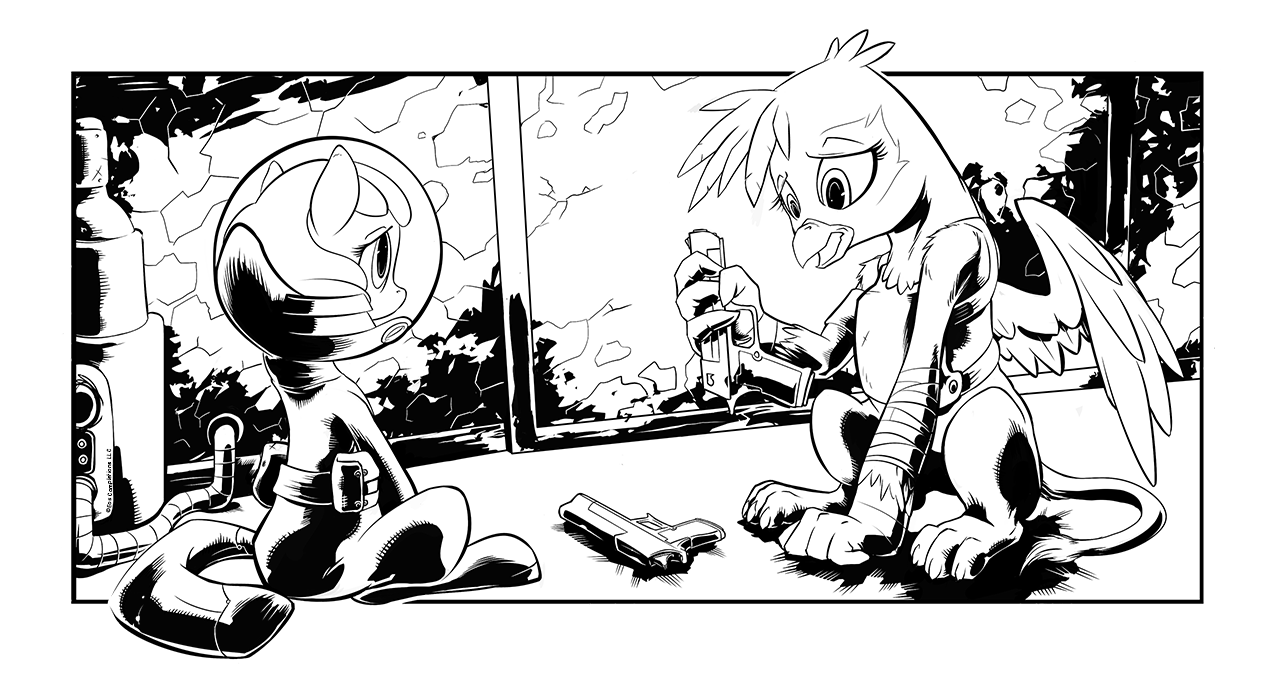
\includegraphics[width=0.9\linewidth]{image06.png}

\begin{intro}
Well, now, uh, Lancelot, Galahad, and I, wait until nightfall, 

and then leap out of the rabbit, taking the French by surprise---

not only by surprise, but totally unarmed!
\end{intro}


\rtpr{``Good evening my beautiful herd! This is Lonesome Pony, and you're listening to Radio 52, the frequency that gives you all the essentials about the Big 52 and nothing else!''}

The evocative tinkling of dueling banjos filled a brief intermission.

\rtpr{``Let's get to work. Have you ever wondered what the sun looks like? Ask the White Apples! Last night, a gigantic ball of light exploded ten kilometers east of Salt Cube City, leaving thunder and devastation in its wake. Luckily enough, along said wake there were mostly radigators and abandoned shacks, but the light could be clearly seen even from Tunnel Town, the Badlands, and the Redtrotters territory. If you think this is crazy, I must warn you that it was just the last act of a night of follies! First we had the launch of a balloon full of ghouls; yes, the very same ghouls that threatened the caravans in the area! The take-off was accompanied by a light and magic show offered by a certain Puppysmiles. Weird name, isn't it? This is not the first time I've had something to say about this gal. Good old L.P. asked some more questions here and there, and guess what he discovered? Yes, she's the same filly from the Carnival!''}

A trumpet erupted in triumphant fanfare.

\rtpr{``So, Lonesome Pony, where's the interesting part? Here it is for all those grumpy `too long didn't listen' busy ponies on the road: no more feral attacks between the Badlands and the Cube!''}

There was the sound of a reloading lever action rifle followed by pair of gunshots and a very manly voice saying, ``\rtpr{Hasta la vista, filly.}''

\rtpr{``Oh yes, I love this one! Two tribes get their problems solved by a foal stuck in a radsuit! Now, I don't need to be a shaman to know that she's heading south, so, what's next? Is she going to reopen the Tunnel? Well kid, if you happen to stop by trade station Badlands on the Marshes detour, pay a visit to your number one fan! We'll get to know the filly inside the helmet! Till then, have some music from the best radio station you can find along the Route.''}

\begin{music}
		``Here's a pony there's a pony
	
		and another little pony
	
		funny pony party pony
	
		pony pony sprite\dots''
\end{music}

\horizonline

\englishdaytimeplace{5}{16:45 P.M.}{165Th Brigade field Headquarters, Salt Marshes}

``Stop that damn music, I can't hear if he's still outside!'' the young griffon snapped at Puppy while shooting her an exasperated glare.

``B-but it's funny! You're a grumpy chicken!'' Puppy frowned and went back to hugging her Pinkie Pie plushie. ``Don't worry, Silky Tail, she's not mad. She's just a bit tired.''

Henrietta the Griffon walked over to Puppysmiles and grabbed the filly's helmet so that she could look her in the eye. ``For the last time, I am NOT a chicken! There's a freaking manticore out there that's pinned us inside this place, and you are doing your most to drive me crazy!'' Her voice broke in a shrill screech. ``I hope that my father arrives soon.'' She sighed. ``Maybe with his help we'll be out of here, and I'll never ever need to see your stupid face again!''

``I'm not stoopid! You're a meanie cat and I don't want to be your friend anymore!''

{\mt ``Warning. Hostile griffon at three meters. Threat level: High.''}

``Aw, shut up, Mister Voice.'' Puppy turned her back on Henrietta in a theatrical display of sulking.

``Shut up mister who? Who are you talking with now?'' Henrietta raised an eyebrow. ``You have a radio transmitter in that thing?'' With a jump, Henrietta was on Puppysmiles, trying to take off her helmet. ``We can call for help! Call my father on 90.08! Codename Blaze!''

Puppy was taken by surprise. ``Hey wait! I have to ask Mister Voice! He lives inside the suit and works all the weird things!'' She tried waving a hoof to shoo Henrietta away, but she was already stepping aside.

``Wait. Mister Voice? That suit talks?''

``Sure it does! This is the best space suit ever! And it is also super smart!'' Puppy smiled proudly.

``Yeah,'' Henrietta snickered. ``I bet it's smarter than you.''

``Sure! Smarter than---'' Her smile became a frown. ``Hey! That's not very nice!''

Henrietta was already laughing. ``I can't believe you fell for that! You're hilarious! Dumber than a banana pajama!'' Henrietta smiled and gave Puppy a bump with her paw.

``H-hey, stop that! You meany-mean chicken! If your dad wasn't that hurt, I'd have already given you a lesson!''

Henrietta froze in place, staring at Puppy. ``My father what? What do you know about my father?'' Hope and fear were mixing on her face in a concoction that made even Puppysmiles aware that her next words needed to be used very, very wisely.

``Uh, last time I saw him he was dead. Maybe he got better?'' She smiled, helplessly lost in childish naivete.

``M-my father\dots died? How do you know that? Where have you seen him? This---this can't be, he's the best around; he can't be dead! You're wrong, this can't be true! Tell me that this isn't true!'' She drew her white pistol and aimed it at Puppy, the yellow line along the barrel pointed directly at her nose. ``Tell me that you're wrong!''

Puppy met Henrietta's wild gaze. She could be a bit slow, but there was no lie in those gleaming pink eyes, just the absolute innocence of a child. ``I\dots I don't know. He wanted me to say to you that he really, really wanted to be here and he was sorry. I ran here in a super hurry to find you because he was really sad and I felt bad for him and I lost my mom too---''

\emph{``Enough!''} Henrietta batted Puppy's helmet with a claw, knocking her against a wall, before curling up on herself, trying to hide her face from the harsh reality. ``This isn't true\dots My dad is the best hired gun ever! He's okay, I'm sure he's heading here right now! Fuck, I\dots I\dots'' A soft metallic sound made the girl open her eyes.

Puppy stood in front of Henrietta. She didn't say anything, but took the black gun with the red line along the barrel from her saddlebag and left it next to Henrietta before going back into a corner of the small room.

``Black Rose.'' She stared at the gun in surprise as she came to realize what she already knew. ``Oh no\dots No, please! This can't be true\dots'' Again, she looked at Puppy. ``Please, tell me this isn't real. Tell me this is a bad dream!''

Puppy frowned and looked down. ``I don't know. If this is a bad dream, then I'll wake up and find my mom waiting for me, so\dots I also hope that this is all just a really long bad dream.'' She sighed. ``But I don't think it is.''

``Fuck\dots'' Henrietta took the gun in a claw, looking at it and extracting her own .45 Auto pistol. They were identical in every detail except for the color. ``How did it happen? Why were you there?'' \emph{Keep flying Henrietta, don't snap now. You learned from the best. You can do better. You \emph{must} be better.}

``There were four chickens fly---''

``STOP CALLING US CHICKENS! We are griffons, and we're better than you filthy ponies! Call me, or another griffon a chicken again and I'll make sure that it will be the last time! Capeesh?'' She held Puppy by the neck, keeping her lifted off the ground while she pressed a gun into Puppy's chest with her other claw.

Puppy's eyes were filled with fear. She tried to break free, but after a quite useless struggle, she simply gave up and began to cry. ``I-I'm sorry, Miss Griffon! I'll behave! Please stop! Please!''

Henrietta nodded and put her down. ``Way better. Now, there were four griffons. Where and when?'' That burst of anger somehow washed away the first shock, allowing Henrietta to focus more clearly on the situation before her.

Puppysmiles talked fast, trying her best not to disappoint the scary griffon again. ``It was earlier. I was going down the road with a friend and they were in the sky. At the beginning it seemed that they were doing a pretty show, but then a lot of them got hurt and they fell from the sky and then they were all dead. I spoke with the last one before he was dead and he told me to come here and give you that black thing and to say to you that he was sorry and that he wanted to go south and then I poked him to make him open his eyes, but he kept sleeping but I tried really hard to wake him! Please don't be mad at me, I really really wanted to make him get better, but he didn't move and then Mister Voice told me that he was dead and\dots and\dots'' She stepped back, gasping for air and putting both hooves above her head in an attempt to hide herself. ``Please stop bullying me! I didn't want to be mean I just wanted to help! I'm sorry!''

\emph{Fuck, she's just a kid.} Henrietta hesitated as her anger began to fade. That foal probably didn't even mean chicken as an insult. Nonetheless someone had to teach her something before she got into real trouble.

``And guess who that someone is,'' muttered Henrietta. Sighing, she patted Puppy's helmet. ``It's cool, really. Call me Henrietta or Henri, okay? You just lack some, uh, style, but don't worry, you'll learn. Now let's find a way out of here.''

``But, but you're mad at me!'' Puppy was still hiding her head behind the hooves.

``No, I'm not mad. Now be a good pony and stand up, okay?''

``But I called you a chicken, and I told you that you were mean.''

``Just don't do that again, okay? I scolded you and now we are even. All right?''

``So, so we can still be friends?'' Puppy tried hopefully.

She sighed. ``Yes, we can still be friends. Now please be quiet while I think of a plan.''

Yes, sure, it was easy to say, maybe a little harder to carry out, but even those simple words were enough to renew Puppy's happy-go-lucky mood. Puppy nodded and sat next to the stairs, while Henrietta took a look outside. The predator had to be hiding somewhere, probably waiting for them to venture out in the open.

``Not good. If only I had something better than my guns. I could hope for a lucky shot, but if I miss\dots'' She looked back at Puppy. ``Hey, you don't happen to have a large caliber gun or some high explosives, do you?''

``I have a rock! It's super rocky!'' Puppy proudly showed \emph{The Rock Of Destiny} to Henrietta.

That made Henri snicker. ``Oh yes, exactly what we need, a rock. Sorry kid, but I don't think that I'll let a stupid rock decide my fate.''

Puppy tilted her head, then looked a bit confused at her favored weapon. ``I don't think that you're dumb, Rock, but now it's better that you go back sleeping.''

``Please! I'm trying to put a plan together here. Stop kissing goodbye to everything you stash in your saddlebags and do something useful like---'' Henrietta hesitated. ``Like, ah, on second thought, just go back and play with Twinkle Sail.''

``Silky Tail!''

``Yeah, that one. Have fun.''

``Okie dokie! The tea will be served in five minutes!'' Puppy sat down on the stairs, taking the stuffed Pinkie Pie from her bag.

``Yes, whatever. Now\dots'' She lowered her voice to a mumble. ``There's no decent cover, and I'm not sure that I can outrun that thing for more than a couple of minutes. We have to face it, but we lack the firepower.'' Henrietta sighed in distress. ``This is ridiculous. Those tanks are full of high explosive ammunition, and we are stuck here with three .45s and a uh, rock.''

In the meantime Puppy sat her doll on a large Flack 8.8 projectile while using another one as a teapot to serve tea. ``Hey, do you want six or eight sugar cubes in your cup? Ah, do you have a cup?''

``No thanks. I think I have a plan,'' she said without even bothering to turn back to Puppy. ``I'll run outside and try to get the manticore's attention. After the manticore starts chasing me you'll sprint to the nearest tank and get inside. You have to be fast because I can't distract that thing for very long. When you're in the tank you have to look for HE ammo. They're big and shiny, like a big can with a pointy head. They should have a red band so they are easy to identify. All right?''

``Uh, yes.'' Puppy looked for a moment at her ``teapot'', then shrugged and put it away. ``You just keep an eye on Silky Tail, okay?''

``I don't think that your doll is going anywhere while we're out. Just go inside the tank, grab the big can with the red line and run back here. When you're done I'll explain to you the second part of the plan.'' Henrietta crouched, readying herself for a jumping start. She needed all the speed she had.

``But she'll be afraid!'' Henri turned around and scowled. That filly was a constant source of idiocy and distraction.

``Puppy, Twinkle Sail is just a doll! It can't be afraid!'' Henrietta walked over to the stuffed Pinkie Pie/Silky Tail, grabbing it and waving it around in front of Puppy. ``See? She's smiling, so she's okay! Maybe when we get back she will throw us a\dots HE Flack 8.8?'' Her eyes focused on the object being used as a chair for Puppy's toy. ``Pardon me. Where did you find this?''

Puppy smiled. ``Soft Air gave me Silky Tail in the Glow.'' 

``No, I mean this one. The 'chair'.''

``Oh that. It was inside a broken super huge metal cart. It's shiny and clean, and I've got plenty of them.'' From the expression on her face Puppy felt that she had to say something more. ``Do you want one?''

Henrietta's left eye went twitchy twitch. ``Okay, great. Part one done. Now for part two.''

``What? But we didn't even---''

``No, just no. I said part two, let's never speak of part one again.'' Her self control was considerably improving. ``Listen carefully. I'm trying to lure Mister Big Bad here into the tower entrance. When the manticore pokes his head in you have to throw the shell into his mouth, and then I'll shoot it. The head goes boom and no more bullies, got it?''

Puppy frowned. ``So, I throw the teapot inside the jaws and the movie ends?''

``The what? Yeah, sure, throw that thing in the manticore's mouth and I'll do everything else. Now get ready and don't be scared, okay?''

``Okie dokie!'' She hugged the shell and hid herself behind the wall while Henrietta cautiously stepped out of the building with her wings outstretched.

Not even a minute later, the sound of gunshots came from outside, followed by the voice of a griffon who was teasing the manticore with a lot of words that Puppy never heard before. She was super double curious about what was going on outside, but she had been told to stay put and wait. Now this was a dilemma. If Henrietta found her out of place, she was going to be really mad, and that girl was really scary when she was mad! On the other hoof, Puppy was sure that there was something totally cool going on just a few steps away from her.

``Maybe just a little peek.'' Outside, it rained lead as beastly roars thundered in the storm of the battle. ``Just one peek won't hurt, right?'' She slowly crawled next to the door, hugging her HE shell and trying to look outside. ``Sneaky sneaky\dots''

``Aw, I can't see a thing! This isn't fair at all---''

Suddenly a blurry silhouette came speeding through the door, rushing to the opposite side of the room and yelling, ``NOW!''

``Now what?'' asked Puppy a little surprised.

\emph{ROAR!}

Snarling and scraping at the concrete, the manticore appeared at the door, trying to get inside, but being held out by its size. Puppy found herself looking into the snapping jaws of a fell beast just a few inches away from her helmet and yelped, backpedaling.

``Puppy, what are you doing? Throw that thing now and dive for cover!'' The urgency in Henrietta's voice danced with the panic in her eyes. ``Move that cutie mark!''

Puppy nodded and tried launching the shell. The high explosive round traced a straight trajectory through the air while Puppy jumped as far away as she could. When the explosive ammunition hit the ground right below the beast's head the griffon opened fire.

\emph{BLAM! BLAM! BLAM!}

Three shots, three hits, three bounces. ``Fuck! Its case is too thick; I can't penetrate it!'' She swore and emptied both pistols against that stupid explosive shell to no avail.

``It's not working!'' Henrietta put away one of her guns and took a third pistol. This one was red with a white line along the barrel, but in everything else it was identical to the other two she had. Unloading the gun directly in the manticore's muzzle, she succeeded in making the monster slow down his assault for a moment.

``I think he's trying to make the door larger.'' Puppy stepped back another couple of meters but now she seemed a lot less scared. She tapped her helmet as if she was pondering the situation. ``He's good.''

The beast was looking at Henrietta with bloodlust in his eyes. It was clear enough that he wasn't going to lurk any longer, even if that meant tearing apart the whole tower. The real issue was that the manticore was actually tearing the building apart. Maybe not very fast, but he was getting there.

``Don't just stand there! Come here!'' Henrietta reloaded her pistols. ``We can still make that thing go boom if only I can hit the detonator. You just stay low, I'll try something!''

``What's a dee-tuna thor?''

Henrietta launched herself toward the manticore, ignoring Puppy's question. With a leap she arrived just a couple of slashes out of the beast's reach and pointed both guns at the shell. ``Say goodbye, Josè---'' It was already too late. She noticed that the predator had his head reclined and his back arched. Henrietta was half feline, so she knew just how much a manticore could stretch. She should have known better than to get so close. The cat had just fallen into the lion's jaws, and he didn't even give her time to swear.

In an instant, the manticore stretched out and struck the griffon with a claw, hitting her in the shoulder and grabbing her with his mighty talons. Henrietta shrieked in pain and instinctively but uselessly pecked and bit at the monster's paw.

Puppysmiles screamed in terror, too. She tried to back away further, but her rump was already pressed against the wall. This manticore was terrible, but, even worse, he was hurting Henri.

For a moment Puppy saw not a manticore in front of her, but a pink metal face with blinking blue eyes.

\emph{Please ‒giggle‒ make this ‒giggle‒ end.}


Puppy's eyes flared with pink flames as she raised her hoof. ``Rock!'' As soon as \emph{The Rock Of Destiny} was in her hoof she launched herself against the beast. ``Let her go! Let her go NOW!''

The manticore immediately spotted the yellow critter assaulting him and instinctively turned his head and closed his jaws on her, tossing his old prey aside. The fangs of the monster closed on her, crushing her with a dry, crunchy sound. Henrietta fought to stay conscious while she staggered across the room trying to reach the stairs. In the meantime the manticore let out a triumphant roar that sealed once and for all Puppy's fate.

``No, no, it's too late\dots Save yourself gal. Don't turn back\dots'' Weakly, she climbed a couple of steps, but the pain was driving her crazy. The manticore behind her was howling in a bloody, ponycidal rage, probably tearing apart and dismembering every limb of that poor corpse. Henrietta took a healing potion and swallowed it all in a single gulp before falling face down, her sight now beginning to fail. Henri tried to turn over to see what was going on and why that atrocious beast kept roaring and howling, but all she could see was a thick pinkish smoke and nothing else. Then the griffon lost her battle against the staggering pain and fainted.

Now please, let's have a moment of silence for the truly unfortunate manticore.

\dots

And this is why rule number one says no biting. Ever. The meat might be spoiled.


\horizonline

\englishdaytimeplace{6}{00:45 A.M.}{165Th Brigade field Headquarters, Salt Marshes}

{\mt ``System successfully rebooted. All functions restored. Diagnostic system is online. Subject 001: Puppysmiles. Female earth pony. Subject deceased, condition stable. All clear.''}

Puppy lazily opened her eyes and yawned. ``But it's still dark outside\dots'' She had the unpleasant sensation of something heavy laying on her back. ``What happened? Where's the chicken? And the big meany kitty cat?''

{\mt ``Analyzing: hostile detected. six meters east. Henrietta. Threat level: negligible.'' A single red dot was blinking on the compass.}

``Silly Voice, Henri is not an enemy!'' The dot turned pink. ``Okie dokie, let's go to---hey!'' She moved her hooves, but this didn't make her go anywhere. Puppy looked down to see that she was hanging from some sort of gray perch. It took more than a couple of tries to break free from the skull of the manticore. The skeleton of the beast had turned the same color as the wall, and seemed to be partially stuck inside of it. It was as if the animal and the wall had melded together. The large head of the beast was open in an eternal roar while his wings stretched out, desperately trying to break free from the deadly cloud that had consumed him.

Puppysmiles trotted over to Henrietta, but the griffon was lying on the stairs, giving no signs of life. ``Mister Voice, is she, you know, uh, dead?''

{\mt ``Analyzing: negative. The subject is unconscious.''}

``Oh. This means that she will be okay?''

{\mt ``Affirmative. The subject is recovering.''}

``Okie dokie.'' That was enough for Puppy. She smiled and kissed Henrietta goodbye through her helmet. ``I'm sorry, but I still have to go, Chicken Girl. My mom is somewhere on the other end of this arrow.''

Puppy trotted some meters away, but then stopped and frowned. Somehow she felt that just kissing goodbye this time wasn't enough. She went back to Henrietta, took the Pinkie Pie doll from her saddlebags, and put it under one of Henri's talons.

``Here, Silky Tail. Look after Henrietta and don't let anything bad happen to her.'' Now it was really okay. Puppy trotted outside and retrieved her scooter.

``Hey, can I has some music?''

\begin{music}
		In the jungle, the mighty jungle,
	
		the lion sleeps tonight!
	
		In the jungle, the quiet jungle,
	
		the lion sleeps tonight\dots
\end{music}

\horizonline

\englishdaytimeplace{6}{10:00 A.M.}{Griffon's Fall, Salt Marshes}

Digging in a marsh without a shovel was already torture by itself, but digging your father's grave in this muddy terrain with your bare claws was\dots No. Just no.

Tears dropped from her beak as she swallowed back the pain. Every time she tried deepening the hole in the dirt it was filled again with murky water, but she continued digging in silence. He could never bear her crying, and he was the most hardened badass mercenary ever. And now he was dead, killed by Talons.

Henrietta dragged the dead body to the shallow hole and pushed him inside. The corpse settled into the mud with a gurgle. She watched the blood-stained feathers sinking in the pool as she tried her best to fight back the tears. Fuck\dots He wouldn't even sink in completely.

``Not fair, man, leaving me alone like this. What am I going to do now?'' Henrietta sighed. She tried being mad at him, if only to have some weapon against her grief, but it was so hard. He was gone, so what now? ``Why you\dots''

Fuck.

Just fuck.

She began filling the grave again with mud and all the stones and asphalt chunks she could find nearby. With the last stone in place, Henrietta stared at where his beak had been visible just moments before. She took out the black gun and hesitated, then put it away again. Instead, she plucked three cerulean feathers from her right wing and planted them where she knew her father's chest would lie forever.

``Tell Mom I'll be fine, okay?''

Henrietta rubbed her eyes with one claw while she rummaged in her bag with the other, retrieving Silky Tail. She looked into the smiling blue eyes of the stuffed doll and tried to smile back. ``I'll be fine.''


\horizonline

\englishdaytimeplace{6}{11:30 A.M.}{Random encounter location, Salt Marshes}

``Hi! I'm Puppysmiles!''

One of the three slavers, a black earth pony, frowned. ``I think I heard that name before. Maybe we should just pass on this one.'' He looked at the other two ponies. They were all well armed, but over the last two days Lonesome Pony kept rambling on about a ghost infesting the northern branch of the Big 52.

``I'm not afraid of ghosts, Dripping Blood, but if a foal scares the shit out of you then just keep an eye on the other slaves.'' The leader of the slavers, a yellow unicorn, glared at his meager haul: a couple of stallions and a foaling mare. Way below the quota. ``Forty Nails, catch her.''

Puppysmiles was a bit uncertain. There were six dots on her compass, but half of them were pink and the other half were red. This had to be more weirdness by Mister Voice. One of the ponies marked with a red dot approached her cautiously and put a hoof on her back.

``Now come with us and don't resist, kid.''

``Okie dokie! Where are we going?'' Puppy smiled with enthusiasm.

Apparently her behavior was quite odd to these newcomers. The nearest pony, a green unicorn, looked over to his boss, who shrugged and encouraged him. ``See? Easy peasy. Put her in a collar and let's move.''

Forty Nails tried to open Puppy's Suit, but he wasn't exactly a Ministry of Peace technician. ``Hey boss, this fucking thing won't open!''

``Uh-uh. I can't take it off too. It's a super stuck helmet. I even tried hitting it but it just keeps repairing itself!'' At last somepony was helping Puppy with the space suit problem, but they didn't seem anywhere skilled enough. ``I think that there is some sort of button to press here and there but they don't work.''

``Shut up, retard.'' Forty was losing patience and decided to go medieval on the whole problem. ``It's clobbering time.'' He held up a hydraulic wrench and brought it down hard on Puppy's helmet, creating an intricate network of cracks that ran across its surface.

The yellow unicorn roared. ``Hey, if you break her head I'll break yours! A dead foal is worth nothing!'' The black slaver simply kept an eye on the other three slaves snickering at the scene.

Puppy stepped back, afraid. ``Hey, that's dangerous!''

{\mt ``Warning. Compass malfunctioning. Warning. Sensor system offline. Warning. Helmet integrity severely compromised. Repair system activated.''}

``Fucking Sun, that's a hard nut to break!'' The green unicorn raised his weapon again, only to see that the cracks in the helmet were already closing. ``What the fuck?'' He hesitated.

``Just tie her up with a rope and let's get going. We'll see to that once we're out of this shit hole.''

Puppy was told to behave, so she behaved while the pretty ponies put a noose around her neck. It was only when they tried dragging her with the other slaves that she began feeling something wrong in the air.

``Hey, I can't leave my ride there!'' She trotted toward her scooter, but the slaver holding the rope stopped her with a sudden jerk.

``Where do you think you're going?''

Puppy kept struggling. ``My scooter! Lemme go!''

Forty Nails snickered. ``Yeah, sure bitch.'' He pulled her close and looked into her eyes. ``You're a slave now. Forget your scooter and everything else. If you want to stay alive, stay put. Got it?''

``Uh, but I have to go there!'' Puppy pointed a hoof south. The green unicorn snorted and hit her on the flank with the butt of his hunting rifle.

``Shut up and open your ears or I'll rape you hard! Rebel ponies are bad commodities anyway.'' Forty turned to the slaver's leader. ``Hey boss, I'm teaching this one a little respect.''

``Don't mess her up or you'll be paying for her.'' The leader shrugged without even turning back.

Puppy frowned. ``I don't think that's a nice word\dots'' She seemed completely unfazed by the first beating, so the green slaver gave her a stronger blow.

``SHUT! UP!''

Puppy was sent flying, landing a few meters away. ``Hey! Somepony could get hurt!'' She got up on her hooves, giving no sign of pain and earning a worried look from Forty Nails.

``B-but what are you? Fuck off and stay down!'' The slaver aimed his rifle and shot two bullets into the foal.

\emph{BLAM! BLAM!}

Two hits, two holes in the filly's chest, and still no reaction. Forty's eyes widened in terror. In the meantime the leader turned on his minion.

``What the fuck are you doing you fucking son of a fucking drug addict! This is the last time you kill a slave!'' The yellow unicorn rammed into the green pony head on, sending him flying through the air.

``No! I'm not gonna die here!'' In a state of utter panic, Forty turned his rifle against his boss and emptied the magazine, blowing off one of the unicorn's legs before he could even realize what was going on. The slave leader fell to his knees, pulling out his assault rifle and spraying bullets all around. The black earth pony that had kept silent until now unsheathed a shotgun but was hit by the raging boss along with one of the slaves and Puppysmiles. The bullets pierced the foal's suit, leaving at least three different holes. It didn't seem to affect her very much.

``Stop quarreling! Please! Hey! I'm talking with you too!'' Puppy tried to restore some order, but this brawl seemed a bit beyond her capabilities. ``You are all bad ponies and you should feel bad! Mister Voice, do something!''

{\mt ``Repairs finished. Containment fully restored. Subject 001 Puppysmiles deceased. Condition stable. All clear.''}

``Not that something! Something else!'' Puppy pouted.

The black slaver staggered, trying to retrieve a healing potion but, before he could, the unwounded stallion slave rammed him, taking his gun and emptying it into his sorry muzzle. The wounded slave fell to the ground, coughing blood while the pregnant mare tried to find cover behind the armed slave.

Forty Nails finally exhaled his last breath. The leader was rapidly bleeding to death, but he didn't want to arrive at hell's doors alone. With the glow of magic, a remote control appeared from his saddlebags. He lay on the ground trying to laugh as he coughed up blood. ``Do not fear ‒\emph{cough}‒ little pon ‒\emph{cough}‒ ponies, you are going to ‒\emph{cough}‒ to precede me.'' He raised his good hoof to hit the detonator for the the slave's collars. The two surviving slaves looked at him in horror.

``No toys for the meanie pony!'' A yellow hoof took the detonator from under the slave leader's muzzle. Puppy was looking at him with her best scolding look. ``I said stop being crazy! I'll keep this thingie until you behave!'' She gave a theatrical pause. ''And I'm dead serious about this.''

He looked at Puppy and snickered. ``I\dots can't believe this. ‒\emph{cough}‒ I heard that story about ‒\emph{cough}‒ the ghost.'' His gaze focused for a moment on the last scratches of Puppy's suit as they disappeared completely before his eyes, ``Hell, you're ‒\emph{cough}‒ fucking scarier ‒\emph{cough}‒ than I could ‒\emph{cough}‒ could ever ima\dots gi\dots n---'' His voice died as his life dripped away into the thirsty wasteland.


\horizonline

\englishdaytimeplace{6}{8:30 P.M.}{Tunnel Town Outskirts, Big 52 N Branch}

``So, when mommy pony loves daddy pony super special much, they write a letter to Princess Celestia and ask for a little foal. You really didn't know that?'' Puppy trotted and galloped all around as she talked.

It had been a long, but luckily uneventful walk through the salt marshes. At last the endless plain of murky pools was behind them, giving way to an area of barren hills. Now it was possible, even in the darkness of the night, to see any suspect movement from a good distance. Puppy's HUD flashed here and there with red dots, but they were mostly wild animals scared by her supernatural presence.

The pair of ponies traveling with Puppysmiles were in a bit of distress. It was the pregnant mare, a milky unicorn by the name of Sweet Flower, who spoke first. ``Well yes, it works more or less that way. You're quite a chatty filly, aren't you?''

``Yup! Everypony keeps telling me that.'' Puppy smiled and completely changed the topic. ``I hope that you get a filly. Fillies are the cutest!'' She lowered her voice. ``Besides, I heard that colts have cooties! It's true!''

Sweet Flower giggled and nuzzled her companion, a brown earth pony named Asso, in the neck. ``She's a little bit right, isn't she?''

Asso laughed. ``I just know that it's going to be awesome.'' He stopped trotting and looked into the distance.

``Here we are, little one. That's the Tunnel.'' Asso pointed a hoof to a small group of lights perched on the middle of a steep mountain wall.

A large bridge, formed by many stone arches, rose from the swamp, climbing directly toward the mountain like a highway to the sky. Puppy's eyes widened in awe at the sight of such a marvelous place. It seemed as if the road shot upward like an arrow of awesomeness and then \emph{bam}, it disappeared in a show of colored lights. Her two companions were way more interested in her. The foal's eyes shone in the dark, a bright pink light that surrounded the helmet in a ghostly halo.

``Okie dokie! So, we go now? Mom is waiting for me somewhere in there!'' Puppy asked enthusiastically, failing to notice the alarmed looks the two gave each other.

``Ah, well, we don't live there, and you need to pay a fee in order to get inside Tunnel Town. We are heading to trade station Badlands. It's a small hub along the detour.'' At that point Asso hesitated, but the mare nudged him, encouraging her mate to speak his mind. After a brief pause, he lowered his eyes and continued, ``I---we have to know this. Are you really a ghost? Some sort of guardian angel sent here to protect children?''

Puppy tilted her head and giggled. ``I'm Puppysmiles, Mister Pretty Silly Pony! I don't know why everypony keeps calling me a ghostie. I'm just looking for my mom.''

``Yes, you\dots you told us that about a million times.'' Asso gave a tired look to his mate and shrugged. ``Well, I guess that is all. We owe you our freedom, somehow, so\dots Thank you? I wish I had something to repay you, but we need everything we have just to get home alive.''

``Okie dokie! Goodbye pretty ponies!'' Puppy waited until her new friends disappeared from sight, then merrily trotted up the bridge toward Tunnel Town.

\clearpage % must

~\vfill


\begin{engnote}
		Level up! (5)
	
		New perk added: Intense Training (2) - Strength ($5 \to 6$) You can has a lotta stuff in your bags!
\end{engnote}



\chapter{Foalsitting}

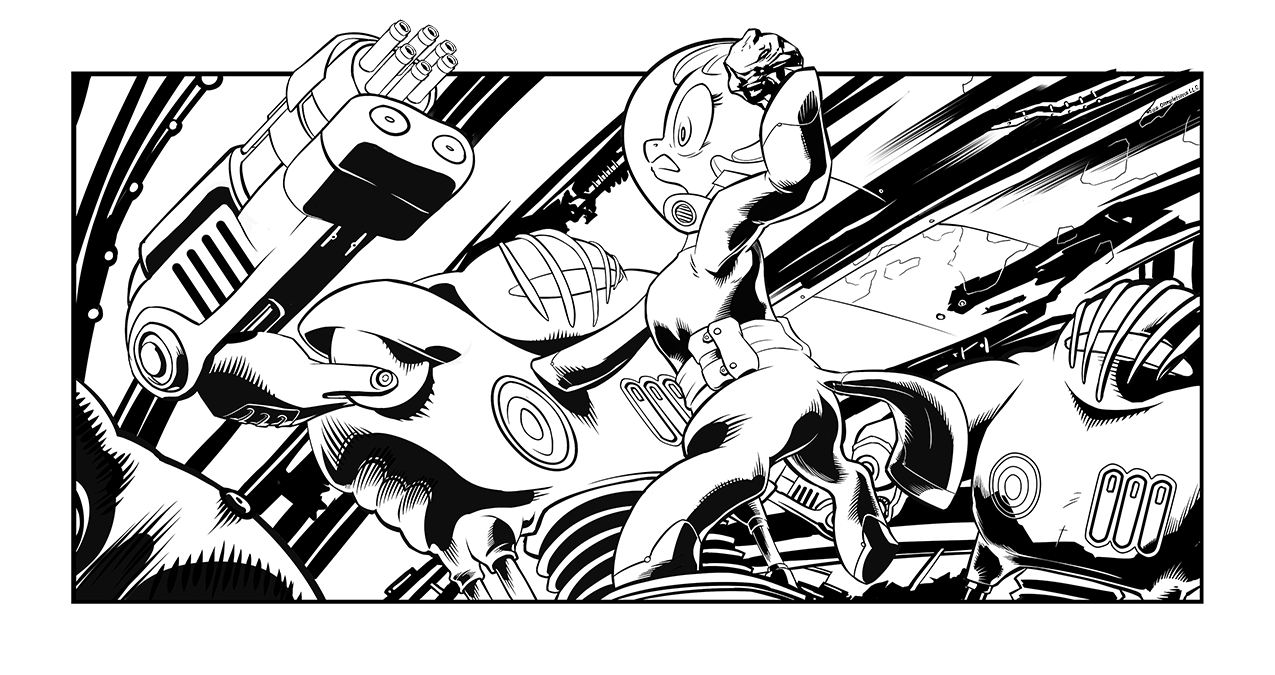
\includegraphics[width=0.9\linewidth]{image07.png}

\begin{intro}
What? These sweet little angels? They'll be no problem at all.
\end{intro}


\englishdaytimeplace{6}{9:00 P.M.}{Tunnel Town, Big 52 N Branch}

Trigger Happy had been a guard for a good half of her life, and she was pretty sure she'd seen everything that could try to get through the Tunnel Town gates. Tonight, she had to admit that she had been wrong, but the fact that all her guards were cowering behind her because of a foal in a funny costume was even more upsetting.

``All right, scaredy-ponies, I'm taking this one. Just relax and, for the sake of my sorry tail, don't shoot blindly.''

She stepped out of the guard post and trotted toward the yellow foal who was surrounded by an eerie pink light. ``Okay, that's close enough. Stop right there and tell me what the hay you are!''

Trigger didn't actually expect the foal to comply, but when she sat down the guard chief felt relieved.

The strange pony rose its hoof and waved it at her. ``Hi! I'm Puppysmiles! Have you seen my mom?''

Trigger Happy frowned. ``Puppysmiles as in 'Puppysmiles the ghost'?''

``I'm not a ghost, I'm a filly!'' she protested. She was carrying something long and red strapped on her back. It didn't seem a weapon, but it was still quite large.

``Let me guess. You zoomed all the way here from Salt Cube City through the marshes on a Red Racer?''

Puppy giggled. ``Nope, I had to trot a bit because the fat unicorn was super boringly slow.''

``The who now? No wait! On a second thought, I don't care.'' Trigger sighed. ``Now I'm coming over. You just don't do anything, ah, ghostly.'' Trigger turned her head toward the guard post just to meet three pairs of eyes that were carefully hiding behind the barricade. One of her guards waved a little white banner for a second. She silently wished for a crew that was less stupid, then trotted toward Puppysmiles.

``Hi! You're pretty, miss pretty pony! What's your name?'' The foal smiled her friendliest smile.

\emph{It's\dots it's just a filly with a pair of glowing eyes, probably caused by a mild case of radiation poisoning.} Trigger chuckled. ``Are you serious? You're the Puppysmiles from the news? The one from the Carnival and Salt Cube City?'' She laughed. ``Oh please, gimme a break!''

Puppy smiled and laughed too. ``Ah ah ah! That's funny! Uh, why are we laughing?''

At Puppy's question the guard chief laughed even louder. ``Name's Trigger Happy, but you can call me Trigger.''

Puppy frowned. ``Ah, can I call you Happy?''

``Sure. Anyhow, I have something for you.'' Trigger took a yellow piece of plastic and handed it to Puppysmiles. ``Here's your pass. A griffon by the name of Henrietta was here at noon. She waited until dusk for you, but then she had to move. Before leaving, she bought you the ticket saying that you were arriving sometime tonight or tomorrow.''

``Uh, Henri was here? Was she all right?''

``Yes, I think. She wasn't very chatty, but I never met a chatty griffon.'' Trigger turned on her tail and trotted back to the guard post. ``Come in! Staying outside this late is unhealthy. We have some bloodwing issues 'round here.''

``What's a bloodwing?'' Puppy asked, trotting behind Trigger.

``If you ask me, they're trouble. Think of them as large flying leeches.'' She snickered and beckoned Puppy inside the guard post. It was a low building surrounded by sandbags and rusted plates of metal. A couple of miniguns were placed in front of the windows overlooking the bridge, and there was a stack of ammo boxes stashed in a corner. Three ponies greeted Puppy with scarce enthusiasm as she followed the mare inside.

``Look alive guys. This is Puppysmiles, the hero of the Carnival. As far as I know she's on our side, so we have nothing to fear.'' Trigger snickered. ``I'd give my cutie mark to see how Lonesome Pony would react if he knew what his \emph{'hero'} really looked like. Anyhow, this is Green Pear, Jammed Gun, and Little Bean.''

``Hi, I'm Puppysmiles!'' She trotted toward the trio of ponies. Since her new friends seemed a bit uneasy, she felt that something more had to be said. ``I'm looking for my mom, and she's somewhere inside the mountain!''

One of the three guards raised an eyebrow and mumbled, ``Well, that could be a problem.''


\horizonline

\englishdaytimeplace{6}{9:45 P.M.}{Tunnel Town, Big 52 N Branch}

``Wow, it's huge!'' Puppy sat in front of the tunnel entrance. It consisted of a large archway high enough to let in both ground carts and air wagons for emergencies or maintenance. The entrance was so wide it could have handled passage from both directions at once. The concrete of the tunnel walls ended abruptly twenty meters into the mountain, where a rusted metal bulkhead sealed it. On the door there was the symbol of a white alicorn, but this one seemed more bulky and manly than the goddesses. Around the symbol ran a motto: \emph{Solaris Inc. ‒ Try the alternative.} Under the company slogan there was a big red symbol, suggesting danger, that occupied most of the door.

``See?'' Trigger Happy knocked at the metal door a couple of times. ``It's sealed. I'm afraid that your journey ends here, little one.''

``But my mom is in there! Look at the arrow, see? It points to the door! I have to go inside the mountain! Open it please!'' Puppy put on her best pout. ``Puppy please, Miss Happy pretty pony?''

Trigger stepped back frowning. ``Wow, those eyes should be classified as illegal military ordinance! Still, I'm sorry, Puppy. There's no way inside the Tunnel. We have tried our best to reopen it, but, as you can see, it won't budge.''

``But I really, really, REALLY have to go there! My mom is waiting for me!'' She stubbornly stomped her hooves.

Jammed Gun tapped his chin with a hoof and muttered, ``I think that TNT once said something about getting inside using the vents.''

Trigger's eyes widened. ``Shush!'' She launched an angry stare at her subordinate before quickly turning back to Puppy, trying to hide a concerned look under a fake smile.

``See? No way inside!'' She tried to hold a poker face, but Puppy was already frowning.

``Uh, vents? What are the vents? Please, I'll do anything. I-I have this!'' Puppy produced one of the tank shells from the military base. This one had a black band around its head. ``See? It's shiny and super duper nice! You let me go inside and I'll give it to you! Deal?''

``Puppy, it's dangerous. I can't let a foal trot to certain death! I'm sorry.''

Puppy stepped back, on the verge of tears. ``I'm not afraid and you're unfair! If it was your mom that was closed inside, you would already be opening that stoopid door! And\dots and---'' She bucked the door. ``I can't stop now! She is there, she \emph{must} be there!''

Jammed stepped next to Trigger and whispered, ``Why not let her in? After all, she's already saved two towns! Besides, I don't think she's just a foal.''

Trigger sighed before she replied. ``We don't know what's going on inside the Tunnel right now, but I'd like you to recall the day the door closed. I clearly remember the ponies trapped inside hitting the door and asking for help, the sound of the guns, and the voices screaming in pain and terror.'' Trigger softly bumped Jammed's forehead with a hoof. ``Look at her. Maybe she's not your average little pony, but she's still just a kid. I'm not sending kids to clear minefields.''

Jammed looked into his chief's eyes. ``Do you think that she'll give up that easy? If she really is the famous ghost, I don't think there's anything we can do to stop her.''

Trigger Happy facehoofed. ``Are you really falling for those fairy tales? Please, get real! She's just a filly with a full enviromental suit and mild radiation poisoning!''

In the meantime, Puppy was still standing in front of the door, muttering to herself. ``I'm not a foal, I'm a big pony! I've made a balloon fly!'' She frowned angrily at Trigger Happy. Suddenly, a new idea popped into her head, making her smile cunningly. ``Say, Mister Voice, what is this vent they are talking about?''

{\mten ``Vent: ventilation system. Device used to circulate fresh air inside close spaces. In the case of a tunnel it consists of a long web of passages that take air from the outside and pump it inside using fans and small ducts large enough to let a single pony crawl through them for maintenance--the more you know!''}

``So, ah, there are other doors to go inside the mountain from where the air gets in?'' asked Puppy, trying to translate what she was just told.

{\mten ``Affirmative. Loading local maps. Solaris Inc. Tunnel n° 2. Analyzing technical blueprints. Warning. Part of the blueprints are not available due to military restrictions. Loading section A01, A02, and A03. Loading maintenance tunnels blueprints. Analyzing. Elaborating route. Maintenance hatch A01-104 set as new waypoint.''}

The pink arrow disappeared from the compass and appeared again pointing to a new direction.

A grin appeared on Puppy's muzzle. Once again she had outsmarted her rivals.


\horizonline

\englishdaytimeplace{6}{10:15 P.M.}{Tunnel Town, Big 52 N Branch}

``And I'm saying that I've never seen a pony survive inside a sealed suit for more than three days! Your 'kid' seems just a bit too fine to be normal!'' Jammed Gun pointed a hoof at the empty place where Puppy was supposed to be. He did a double take, looking at where he was pointing and realizing that something was missing. Something the size, shape, and color of Puppysmiles. ``What the hay?''

Trigger Happy jumped on her hooves, looking around frantically. ``She was here a minute ago! Why didn't you keep an eye on that filly?''

``Oh, now \emph{I} have to watch after the glowing, yellow pony? And what were you supposed to do?'' Jammed stopped and snickered. ``See? It's just like I was saying, you can't stop the Ghost of the Big 52.''

``She's not a ghost, so stop blabbering.'' Trigger Happy waved a hoof, dismissing the idea, but her companion continued talking.

``Now please, Happy, listen to me for a moment. This place is getting worse every day. When we were kids we used to play outside, and the Big 52 had way less slavers and bandits. The tribes were strong enough to keep order and make everypony feel a little safe.'' He sighed. ``Don't you miss those days, Happy?''

She looked down, sadness filling her eyes with a dim shadow of tears. ``Yeah, but at that time it was easier. The tunnel was still open, and Sun City was a civilized place. Now the Big 52 is just a bunch of detours and dangerous trails.''

``Yeah, I know\dots so I was wondering. They say that everything has a spirit, right?'' Jammed Gun was trying hard to explain a thing that was quite clear in his head, but not that easy to put down in words. ``It's like a city. A city is more than the ponies that live in it. The efforts of the community and the hopes of the families sustain each other, feeding a common will that makes you feel as if the whole place is alive.''

``Yeah, it's called community. So what?'' Happy looked at Jammed with a dubious expression. ``I hope you're really going somewhere with this, because we have a lost filly right now!''

``So, even the Big 52 is something like that, right? I mean, The Redtrotters, the White Apples, the Sand Sweepers, and all the other tribes. Maybe they're separated, but they all live on the same long route from the Ridges to Emerald Shores. We are all on the same road, and we all are citizens of the Big 52.'' Jammed Gun raised a hoof pointing north, then arched to the south with a slow movement. ``Salt Cube City belongs to the White Apples, yes, but the Big 52 belongs to everypony that lives along it.''

``This is a very poetic idea, but I still don't see how this is going to help us find Puppy.''

``I'm almost there. We both had that feeling. You know, that the Big 52 is dying. Slowly but inexorably sliding into the same horrors as the rest of Equestria. And suddenly\dots bang! This Ghost appears and starts solving problems that vexed us for years.''

``The Redtrotters were slowly giving up. The Carnival was killing more than a foal per year. It was killing hope. Once I heard a trader say that the mares of the tribe refused to have foals because they were scared to lose them. And the ghouls? Do you know how many caravans traveled only as far as Exchange Station Badlands because making the trip to Downtown wasn't worth the additional escort?''

``Well, yes, okay, but I don't think that a foal can---'' 

``And I think she can.'' Jammed was dead serious. ``Think about that griffon today. Have you seen her eyes? She had this\dots light. As if things for her had sucked for a lifetime, but finally they were beginning to get better. She had hope, and she showed gratitude. Think about this, Happy. How many ponies in this sinkhole value gratitude? Maybe several years ago it was still common to think of other ponies as something other than a potential threat, but nowadays if you don't have the pass you aren't even given a chance.'' Jammed paused for a moment, but now Trigger was listening carefully and didn't interrupt him.

``And now she needs to get into the Tunnel. Maybe she is just a lucky foal, or a dead one, but---but I want to believe that she's something more. Okay, maybe she's not the Stable Dweller, or Security, but she's all we got down here. Just the good old Big 52 trying to fix things by herself.''

Trigger Happy sighed. ``You are a dreamer and a silly pony, Jam. If you have a problem you can't just wait for somepony else to come and solve it for you. You have to face it and work hard in order to earn something.'' She looked away at the ever-clouded sky. ``But I have to admit that in one way, you're right. That filly doesn't know when to give up. I think I know where she's headed, and Luna curse my soul if I'm letting her wander into trouble.''


\horizonline

\englishdaytimeplace{6}{10:15 P.M.}{Solaris Tunnel, Tunnel Town}

A metallic sound echoed through the ventilation ducts. The whole place was pitch black except for the dim light from Puppy's eyes and the helmet's HUD. For her it was more than enough to see where she was going. After all, she was following the arrow. She couldn't be wrong!

``When I find Mom, I'm hugging her super strong. Then she'll kiss me and we will be together forever.'' She was reviewing the vital passages of her new plan. ``Because this time she didn't move away, right Mister Voice?''

{\mten ``Negative. There is a 99.9\% probability that your female parent will not be present or in condition to---''}

``Hey, don't even try that! A positive attitude is everything.'' Puppy stopped for a moment and looked around. She could've sworn she heard something. ``Hey, did you hear that? Like somepony calling?'' She took a deep breath. ``I'M HERE! WHERE ARE YOU?''

The sound of Puppy's voice echoed for a lifetime in the dark and lifeless tunnels before dying. A distant voice seemed to reply, but Puppy couldn't hear it very well.

``Where is this voice coming from?''

{\mten ``Analyzing. White noise and distortion are too high. Impossible to determine the source of origin.''}

``Oh well, then let's move.'' Trotting away, Puppy found herself looking down from a grate. Just below her there was a black and bottomless void ready to devour anything.

``Uh, why is the arrow pointing down now?''

{\mten ``Loading instructions. You need to reach the main tunnel ground level in order to proceed. Maintenance grate A01-001 is the nearest passage to reach the next section of the tunnel.''}


\horizonline

\englishdaytimeplace{6}{10:15 P.M.}{Tunnel Town, Big 52 N Branch}

``I don't give a fuck about your opinion, Jam! Now give me the light helmet and help me with that checklist.'' Trigger Happy was wearing a worn-out maintenance suit equipped with a wide variety of tools.

Jammed Gun sighed, trying to appear annoyed. It wasn't hard to sense that he was worried to death. ``As you wish, Happy, but please, come back\dots''

Trigger snorted and looked away. ``The list.''

The stallion sighed again and shook his head. ``Rope.''

``Check.''

``Batteries.''

``Check.''

``Canteen.''

``Check.''

``Shotgun and slugs.''

``Check, check.''

``Common sense.''

``Che---hey, stop playing around!''

Jammed Gun snapped, unable to conceal his feelings any longer. ``And you stop trying to kill yourself, Happy! You're a good shot and an action pony, but you're still a pony! You could get killed, and I don't want to lose you!''

She cocked her head. ``Lose me? What do you mean by that?''

``I mean that I love you, Trigger Happy! Since we were little more than foals! Why do you think I enrolled into the guards instead of keeping Pa's tavern? Please don't go\dots or at least let me come with you!''

Trigger tilted her head, frowning. ``You mean\dots you had a crush on me for, like, twelve years and never said a single word? Even when Black Hat and I---'' Trigger shook her head. ''You're kidding me. This is another fucking joke, isn't it?''

Jammed Gun sat down, lowering his eyes. ``I wish it was, but you can be really cruel sometimes. And I'm a shy guy, you know? But I can't just watch you kill yourself over a ghost.''

``She's not a ghost! Why must you be so stupid? She's a little foal, and she is in danger!'' Happy grimaced. ``Since she's not coming back, I'm going inside to get her, and I'll spank her so hard that she will never do something like this again!'' She paused for a moment. ``Oh, and I'm sorry, but after Black Hat, I'm more into fillies than colts. Uh, we should talk when I get back. Is the list done?''

Jammed's jaw fell open in shock. It took him a while to process what she'd said. Slowly, he regained his composure and nodded in her direction.

``Sweet, I'll be back soon.'' Trigger crawled inside the maintenance tunnel, disappearing into the darkness.

``Great. I got dumped. Twelve years to find the guts to spit it out, and I got dumped! Fuck, I'm out of here. Maybe Little Bean didn't finish that Wild Pegasus.'' He turned on his tail and walked away, stopping one last time only to whisper, ``Please, come back in one piece\dots''


\horizonline

\englishdaytimeplace{6}{10:30 P.M.}{Solaris Tunnel, Tunnel Town}

{\mten ``Warning. You are doing it wrong.''}

Puppy was jumping up and down on the ventilation grate. After a minute of this treatment it had begun to crack. A bolt detached from the frame and fell into the black nothingness underneath. ``Don't worry, when the grate falls I'll jump away super fast! What could ever go wrong? After all, I'm Space Captain AndromedaaAAH!''

\dots

\emph{THUD!}

\dots

\dots

``Owie.''

{\mten ``Repair spell activated.''}


\horizonline

\englishdaytimeplace{6}{10:30 P.M.}{Solaris Tunnel, Tunnel Town}

Trigger Happy slowly crawled down the maintenance tunnels, searching for some sign of Puppy's passage. She was quite sure that Puppy entered the tunnels from the same hatch she did, but that place was a hell of a labyrinth. Lucky for her, though, she had a stick of chalk and a decent light source.

Passing above a ventilation grate, the mare stopped to look down in the main tunnel fifteen meters below. The grate creaked dangerously under her weight, but held.

``Sweet mother of Luna.'' Right below Trigger, not far from the metal doors that separated the inner tunnel from the town, were piles of bones that had amassed on the ground. They were the only surviving remains of the more than two dozens ponies that had been corralled there and executed on the spot. It was horrible.

Trigger could still remember the day the doors closed. It was an ordinary day only ten years ago. She had just begun her career as a town guard and still had to take tunnel patrol duty, though of course she had already been through them many, many times before. The passage connected Tunnel Town with Trade Station Tunnel South. It was the only way to get past Sugartop Mountain besides the pass, which was dangerous on clear days and practically suicide when it rained. If you wanted to reach the northern branch of the Big 52 from the south, you had to trot six kilometers underground, and pay good caps for it.

Then, the doors slammed shut.

There were no warnings, nor signs that it was coming, and, worst of all, there seemed to be no reason. The thick, gigantic bulkheads simply fell from the ceiling and sealed the tunnel with all the ponies that were inside at that moment. For about an hour ponies on both sides of the doors tried to open them, but suddenly those inside started screaming and beating on the metal, begging to be let out. It was at that point that there came the gunshots. The roar of two dozen machine guns that put a stop to the screaming.

After that day, only silent darkness dwelt in the tunnel. At first a couple of adventurers tried to get inside and hack the doors, but they never came back. With time the ponies of Tunnel Town resigned to this turning of events and worked hard to make the pass a little safer. A lot of ponies died trying to exterminate the predator's nests along the path, and they built a couple of shacks on the trail, but the caravans today were less than a fifth of the ones that used to pass through when the Tunnel was open. Tunnel Town was slowly dying.

Those skeletons below were just the first victims of this senseless tragedy, and maybe they were also the lucky ones. At least their end was fast.

Suddenly the sound of machine guns echoed in the tunnel. Trigger rubbed her ears to be sure that she wasn't hallucinating, but the guns kept firing.

``Fuck. I'm too late.''

\emph{That poor filly. Why did Jammed have to make me lose so much time? If I had been faster Puppy could still be}---``Wait, why are they still firing?''

The machine guns were still roaring in the distance as if they were fighting something rather than simply slaughtering it. Maybe the foal found some shelter and the security turrets couldn't hit her. Maybe it wasn't too late! After all, as long as the guns fired, it meant that Puppy hadn't been killed.

Trigger took the screwdriver and the rope from her utility saddle. ``Hold on little one! Big sis is coming for you!''


\horizonline

\englishdaytimeplace{6}{10:45 P.M.}{Solaris Tunnel, Tunnel Town}

Puppy trotted toward an abandoned cart in the middle of the road. She tried sniffing it, but it was a bit difficult since she was wearing a helmet. ``This place is full of cool stuff like food, toys, and those noisy guns that everypony is carrying around these days. Maybe it's some sort of super big closet.'' Puppy shrugged. ``Oh well, let's find Mom.''

``STOP RIGHT THERE, CRIMINAL SCUM!''

A boisterous voice echoed in the tunnel that made Puppy turn her head. ``Oh, hi there! I'm Puppysmiles!'' A robot as large as a pony in heavy armor stood in front of her. It had the Solaris Inc. brand on its flanks, and a couple of firearms attached to each side.

``SURRENDER NOW AND BE ANNIHILATED!''

% Puppy giggled. ``Silly robot, it's surrender \emph{or} be anni---any\dots eenie\dots whatever.''

Puppy giggled. ``Silly robot, it's surrender \emph{or} be anni---any\dots eenie\dots\\ whatever.''

% NOTE: force to break line

The robot opened fire, hitting the cart and Puppy with no less than a dozen projectiles. Now, a rapid fire gun uses small caliber bullets that have decent piercing power, but those are nothing special when it comes to dismembering things.

Puppy looked down at the holes in the suit as a thin thread of pink smoke snaked out into the air. ``Hey, I was using this space suit! Oh, I get it now. You're a bullybot!'' Raising a hoof, she stared at the machine. ``I don't like bullybots. Rock.''

The security bot sprayed another salvo of bullets at the filly who charged it with \emph{The Rock Of Destiny} floating at her side. When the guns stopped to reload, Puppy jumped at its head, tearing into its face plate with all her might. She was getting good at this hitting thing. In fact, after just three consecutive strikes in the same place, the glassy visor of the robot cracked, revealing its sensor bay, which was then destroyed in a single hit. The machine stopped functioning almost immediately.

``And stop bullying fillies, dumb robot!''

``STOP RIGHT THERE CRIMINAL SCUM!'' Another two sentinels opened fire at Puppy, though they were so far away that they mostly missed her.

``Moar bullies? Very well, I have something for you too, stoopid bullies!''

A hail of bullets almost tore away one of her hind legs, but with Puppy, almost wasn't good enough. The wound simply slowed her. ``Don't you know that I'm a nice filly and I always try to behave? You're making me not behave! I'm gonna get in trouble for this!'' With \emph{The Rock Of Destiny} in her hoof, she was already on the second robot, cracking its visor.

Three more sentinels arrived, emptying their barrels into the filly, but she was way smaller than the robots. Their friendly fire destroyed another machine with the sheer volume of bullets alone.

``Aren't you listening? Are you stoopid or what?'' Puppy jumped on another robot, springing off the carcass of her last victim. Tracers zipped through the air, and her, while the suit rang every sort of alarm. Puppy? She didn't care. She just kept going.

``Fillies are made of sugar!'' Landing on the robot's face, she hit the top of its head, piercing it with her weapon in just five strikes. In the meantime, one of the two remaining robots ran out of ammo.

``SPICE!'' Puppy put a hoof inside the hole she had made using \emph{The Rock Of Destiny} and pulled out all the cables and circuitry she could. Something in the robot crackled and sparkled as it emptied what was left of its magazines all over the place, destroying the remaining two sentinels before shutting down itself.

``AND!'' \emph{Clank.} ``EVERYTHING!'' \emph{Clank.} ``NICE!'' \emph{Clank.}

At last she found some time to breathe while the smoke of the burning wreckage dispersed a little, mixing itself with the pink gas that leaked from the holes in her suit. A pink goo dripped from the larger tears, evaporating as soon as it touched the ground and mixing again with the cloud around her. Her ears still rang with the sound of firearms.

The pink cloud as usual didn't dissolve, forming a thick curtain of smoke around her instead and slowly beginning to vanish only when the holes in the suit were mended. The repairing was almost done when a familiar voice called Puppy's name.

``Hold on Puppy! I'm almost there!'' The sound of galloping hooves echoed in the large gallery, and in the eerie pink light cast by her eyes, Trigger Happy's silhouette appeared.

``Hi, Miss Pretty Guard Pony! Did you fall from the ceiling too?''

Trigger ignored Puppy's question and rushed to her, hitting her on top of her helmet. ``You stupid, stupid\dots silly pony!'' Tears ran along Trigger's muzzle. ``You're alive, thank Celestia. I was so worried! Why did you run away?'' Happy hugged Puppy. ``Now, we need to go back to Tunnel Town, since your mom can't be here, see? There are just abandoned carts and one, two, three, four-five-six destroyed sentinel robots?''

Trigger blinked, a bit stumped. ``You just single hoofedly destroyed\dots six sentinels?''

``Uh, please don't tell mom?'' Puppy's eyes were two watery pink lights in the darkness. ``Puppy please?''

``Are you kidding me? How did you do that?'' She pointed at the carcasses. ``I mean, six sentinels and not a single scratch?''

Puppy showed Trigger \emph{The Rock Of Destiny.} ``Ah, they were bullying me. I told them to quit, but they had those noisy things and kept being mean. Mom doesn't want me to beat other ponies, so please when we find mom don't tell her!''

Trigger studied the damage on the robots. ``These three were shot, but the other three you \emph{actually} stoned to death.'' Happy stared at Puppy. ``What are you?''

She tilted her head, a bit perplexed. ``I'm Puppysmiles?''

``Please, give me a break! I heard the firefight from the tunnel's entrance. You can't just stand there unwounded and smiling like a---a ghost?'' Realization hit Trigger Happy like a ten-ton anvil. She wasn't an educated mare, but she had heard a lot of stories from the traders and their guards. ``You, you're a Canterlot Ghoul!''

``Uh, yes I'm from Canterlot. Actually from Clover Leaf Terrace, but even if it's downhill it's still Canterlot, you know?''

Happy backpedaled another couple of meters as she noticed the last ribbons of pink smoke vanishing in the dark air and suddenly felt very, very itchy. In a rush of panic she downed a healing potion in a single gulp and backed off even farther.

Puppy looked at the unicorn and frowned. ``Ah, is something wrong, Miss Happy pretty pony?''

``This---this is ridiculous. You shouldn't be here. You shouldn't be talking with me now!'' Trigger's eyes betrayed her fear. ``You're just a, a---''

\emph{A what? A monster? A walking dead? A ghost? Shut the fuck up, Happy, she's a kid. She talks like a kid and acts like a kid. I came all this way to save Puppysmiles, and I won't go back without this filly.}

Trigger found the courage to put on a smile for the perplexed filly. ``You're just a little lost, but I'm sure that I'll figure out a way to help you if we go back to town.''

``But I can't!'' Puppy stomped a hoof on the road. ``Mom is here, and the arrow says that I must keep trotting in that direction! Please don't take me back, I'm almost there! I, I \emph{need} my mom!''

``I\dots I don't know. If this is really so important for you, I guess that if you promise to be really cautious, then we could try to go a little further. There were some other destroyed sentinels along the tunnel, so maybe these were the last functioning ones.''

``Yay!'' Puppy jumped all around like a spring toy.


\horizonline

\englishdaytimeplace{6}{11:00 P.M.}{Solaris Tunnel, Tunnel Town}

{\mten ``Please state your identification code and personal password.''}

This had to be the mother of all the sentinels. It was at least as tall as three ponies, and had a payload of weapons that made the average steel ranger look like a toy. Hell, Trigger Happy couldn't even name some of the weapons that thing had.

``We should go back, Puppy.''

``No wait! I know this guessing game! It's a genie!'' The foal cleared her voice, ``FT\dots 0\dots 0\dots 1\dots 6\dots 5\dots RD\dots C\dots 1\dots G\dots A ''

There was a long pause. Trigger readied herself to grab Puppy and run like she'd never run before.

{\mten ``Please, state your pass code for this ID.''}

She smiled and declared merrily, ``Hi! I'm Puppysmiles!''

Without even waiting for a reply, Trigger hauled Puppy on her back and started running. ``Please holy Goddess of Acceleration, don't fail me now!''

``Weeeee!'' Puppy was not exactly sure of what was going on, but she was riding a pony, and riding a pony was always fun.

{\mten ``ID accepted. First Class Technician Rainy Days. Access to maintenance section granted. Please do not enter into red marked areas without a Solaris Pass Card.''}

Trigger abruptly stopped, nearly sending her passenger flying across the tunnel. Puppy grabbed Trigger's neck and the two ponies found themselves looking into each other's eyes. Puppy was smiling.

``That was fun, let's do it again! I like piggyback rides! Hey, why are you putting me down?''

She sighed, patting Puppy on the top of the helmet. ``Don't worry, I'll give you another ride, but now I guess that the sentry is letting us go inside.''

``Well, \emph{duh}, sure! I said the magic words!'' Puppy trotted to the metal doors behind the towering robot and tried pushing them. As soon as she touched the metal, the reinforced doors slid open, revealing a corridor lit with dim, flickering lights. A distant voice repeated a long sequence of emergencies in a dull tone.

{\mten ``Warning. Primary power source cut off. Emergency shutdown procedure engaged. Warning. Intruders between sectors A01 and A03. Warning. Security robots not responding. Warning. Comm Station offline. Warning.''}

Puppy sighed. ``Aw, another whinybot.''

``Come again?'' Trigger tilted her head.

``You know. Whinybots.'' The blank stare from Trigger made Puppy sigh. ``I really have to teach you everything! There are three types of robots. Funbots, they are friendly and funny, like Miss Voice or Questioner. Then there are bullybots that are nasty and not so funny. Usually I have to break those ones and I really, really hope that Mom won't spank me for this. And there are whinybots. They can only whine because everything is wrong, like Mister Voice and---''

{\mten ``Negative. I am not whinybot, I am an advanced pony-machine interface designed for---''}

``Yeah, sure, I was talking with Happy, could you please wait a moment?'' The voice from the suit stopped while Trigger Happy stared at Puppy in disbelief.

``You\dots you're wearing a talking suit?''

``Yeah, and he's smart, but don't even try that joke smarter than you and then I say yes and then you laugh!''

Trigger frowned. ``Hey, what kind of pony do you think I am? I was just surprised, that's all.''

``Uh, okie dokie then. This is a super smart space suit that talks and tells me where my mom is. I follow him and usually find a lot of friends and some not-so-friendly ponies, but we still have to find Mom. Maybe this time we'll be lucky. Oh yeah, his name is Mister Voice.'' Puppy smiled, waiting for her reaction.

Trigger nodded weakly. ``Uh, yeah, whatever. So, that thing works more or less like a very large PipBuck. I guess this explains a lot of things, like how the hay you knew where the ventilation hatch was.'' She sighed before continuing. ``All right, little one. Where to now?''


\horizonline

\englishdaytimeplace{7}{1:00 A.M.}{Solaris Tunnel, Tunnel Town}

Long story short, it took a little over an hour for the two ponies to reach an old rusted generator room and make the geothermal turbines run again. Luckily for them, restarting the turbines was just a matter of reconnecting cables that had been cut by a fallen steel beam. With some salvaging and jury rigging, mostly done by Trigger Happy, the electricity was now running along the cables again.

``Okay, let's see. Yes, the elevator is working again. We can go up.'' Trigger cleaned the sweat from her face and pushed open the elevator doors.

``Yay! I'm going to see Mom! Thank you thank you thank you so much, Miss Happy!''

She smiled weakly. She didn't believe that Puppy's mother really was somewhere near this place, but she was proved wrong so many times today. \emph{Maybe a little positive thinking is just what we need after all.} ``Good, we just have to hit the attic and see for ourselves.''

The elevator ran for more than a minute, tormenting the two passengers with lousy music that made Happy regret restarting the generators. When the doors opened again, there was a room with a whole wall made up of windows and large screens everywhere. It was the tunnel maintenance control room, and it hung above Sugartop mountain from a panoramic position that let Trigger see all the northern plains, even in the darkness of the ever-clouded night.

Puppy trotted around for a bit. It wasn't a very large place, but it had a lot of metal tables with terminals on them, as well as large maneframes stuck in a wall that could have actually hidden a crouched pony. The room was clearly empty and Trigger wasn't completely sure that just calling Mom louder was going to make her magically appear.

``Puppy, I\dots I don't think she's here.''

Puppy turned her head toward Trigger, and for a moment she felt a block of ice paralyzing her guts. Those eyes. So angry, so desperate, so\dots empty. It lasted for just a moment, but now she knew exactly how Puppy had been able to overcome six sentinels with a rock. \emph{Never cross her if you value your life.} ``Uh, I mean, maybe she moved away?''

Puppy lowered her eyes and sighed. ``Yeah, maybe. Last time she left some voice thingie that said she was coming here. Miss Voice could help a little with that.'' Puppy was now trying to smile again. That little ghost was full of anger, but she fought it with optimism. \emph{How long will this last? How long before she loses hope? And what will happen then?} ``Mister Voice, we need a professional. Call Miss Voice.''

~\vfill

\begin{engnote}
		Level up! (6)
	
		New perk added: Hard Rock!  - Okay you got a rock, now show us how bad you are with it. When using rocks, you ignore an additional 10 points of a target's damage threshold
\end{engnote}



\chapter{Past Dreams}

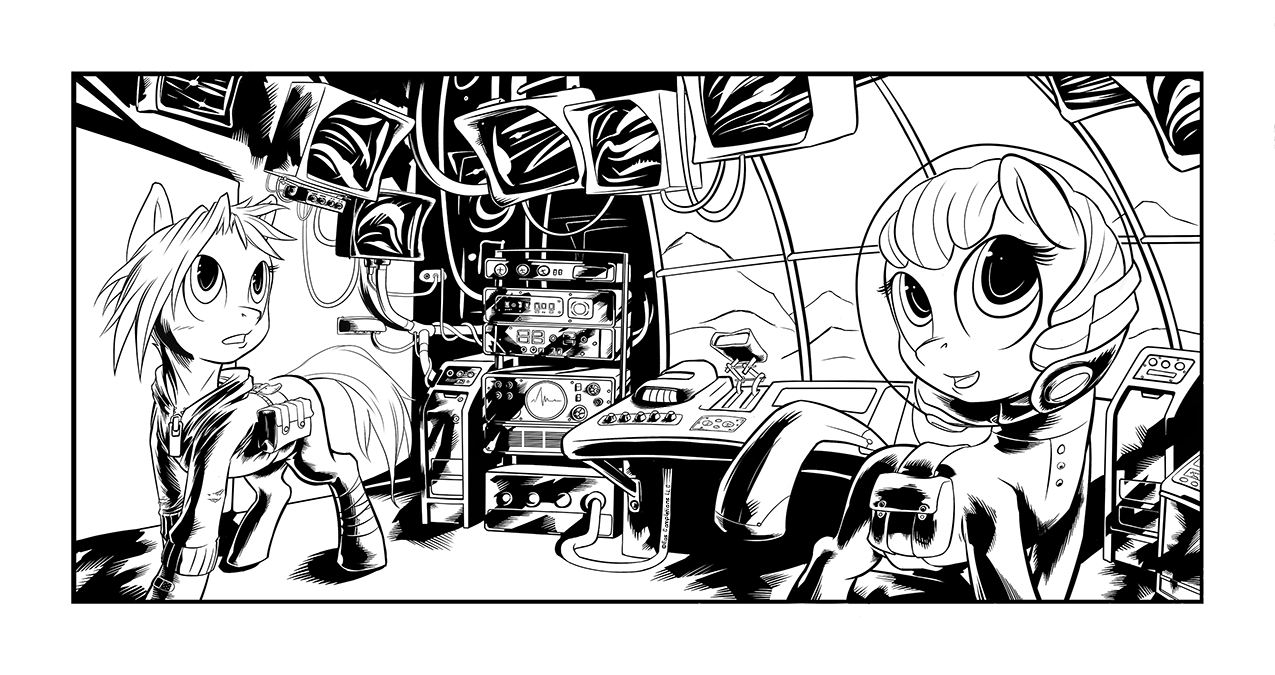
\includegraphics[width=0.9\linewidth]{image08.png}

\begin{intro}
The darkness and the shadows they would always make me fro-own!
\end{intro}


\englishdaytimeplace{7}{3:00 A.M.}{Solaris Tunnel, Tunnel Town}

Trigger Happy yawned and looked down at Puppy, who was playing peacefully on the command room floor. She was moving a toy cart around while making noises with her mouth. She put a couple of bottlecaps on the cart and placed it next to an empty bottle of sparkle cola, then dumped the bottlecaps on the ground and replaced them with the bottle.

``I can has super special minty flavor? 'Kay thanks, bye.'' She was playing quietly, as if she was worried about disturbing somepony by making too much noise.

\thpr{How can she be like that? Just ignore all the horrible things she's seen, and simply sit down and play, like a common foal?} ``Hey, little one, how is your friend doing?''

Puppysmiles didn't look away from her toys as she answered. ``Dunno. She told me it might take a long time, but I have to wait here or it won't work.'' Now she was building some sort of fence all around the empty bottle using\dots

Trigger raised an eyebrow. ``Say, why are you carrying \SI{9}{mm} bullets with you?''

``Oh, these ones? They're pretty and shiny. And it seems that they are needed to use the nine mail mint argon.'' Again, Puppy didn't even raise her eyes.

``The what now?''

Puppy waved a hoof and said in a loud voice, ``Noisy thing.'' A badly damaged \SI{9}{mm} semiautomatic pistol floated up to her hoof, making Trigger step back and take cover behind a terminal.

``Hey, who gave you that? It's dangerous!''

``Nah, it's just noisy. I don't like it very much, it seems more like a colt toy to me. Maybe if it was pink\dots''

Trigger smiled nervously. ``Yeah, Puppy, it's not a very fun toy. Wanna exchange it for something better?''

This gained Puppy's unconditional attention. Her gleaming pink eyes burned into Trigger with expectation. ``Sure, what have you got?''

``Uh, what about a cool pair of sunglasses?''

``Yay! Sunglasses! No wait.'' Puppy frowned. ``I can't use glasses with this stoopid helmet.''

Trigger facehoofed. ``Right. Sorry little one, what was I thinking?'' She went back to digging around inside her saddlebags. ``What about an almost complete \emph{Bridle Gossips} magazine? It's full of pictures of pretty ponies, and there are Fluttershy photos too.''

Puppy trotted to Trigger, took the magazine, looked at it for a moment and smiled. ``I like this one, it's full of pretty ponies! Look at this one. I know her, she's Pinkie Pie! And this one is Rarity and---oh, look here! There's Rainbow Dash too! I lovelovelove Rainbow Dash! She's smart and super cool and she can make the sky go boom! When I'm big I will marry her! I like the picture book, gimme gimme gimme!''

Trigger tried to suppress a chuckle. ``I think we can talk about that, but you have to give me the bullets too.''

``Uh, okie dokie! And what can you give me for the big ones?'' asked Puppy, retrieving a couple of 8.8 Flack AP shells from her inventory.

The mare sighed. This was going to be complicated.

\horizonline

\englishdaytimeplace{7}{3:00 A.M.}{Sugartop Cafe, Tunnel Town}

Sugartop Café was dark and full of smoke, as it usually was late at night. The place was largely deserted except for a couple of drunk ponies nursing the dregs of their bottles, a griffon keeping to himself in one corner, and a pony with a guitar who was largely hidden beneath a sombrero. The bartender was already ``cleaning'' the floor with a bucket of dirty water and a mop that had seen better days, but Jammed Gun couldn't care less.

``Another!'' He said weakly as he raised his empty glass, rattling the blue straw sticking out of it. It remained empty. ``Hey, son of a mule, I said another!'' Waving the glass faster didn't do the trick either. This was upsetting.

The bartender, a silvery stallion with a black mane, trotted to Jammed's table and put down a Sparkle-Cola. ``Hey, big bro', keep it down please. I've got clients sleeping upstairs.''

``Shut the fuck up, Blackie,'' muttered Jammed, ``and fill the glass with something strong. I can't believe she dumped me!''

Black Hat sighed and pushed the Sparkle-Cola against Jammed's muzzle. ``Oh please, Jamie! Forget her already and go to bed. Look, you can use my place upstairs, okay? Just stop drinking. It's not helping you at all.''

Jammed tried to look at his brother's face, but his head didn't want to move from the table. ``You know the bar is half mine, right Blackie?''

``Yes, but you only come in here to mope about your life while I have to deal with the customers and keep it clear of the noisy whiners who drive away the few ponies that actually pay for their drinks!'' Black Hat stomped a hoof on the table. ``Honestly Jamie, you can be a royal pain sometimes.''

Jammed Gun waved a hoof, trying to shoo his brother like an annoying fly. ``Fuck off, Blackie. I feel like manure and I don't want you around. I want booze.''

``I think that instead you should take a trot 'round the town, Jamie. Staying here won't make you feel better.''

``Shut up and give me another wild pegasus, Blackie.'' Jammed raised the empty glass again, keeping his face on the table. ``How could she?''

At last Black Hat snapped. ``Oh, c'mon, Jamie, let's get real! It's Happy we're talking about, the bitchiest mare I've ever kno---'' \emph{SMACK!}

Jammed Gun rubbed his right hoof as he looked down at the prone form of his brother laid out on the bar's floor. ``You know what, Blackie? You were wrong. Staying here made me feel better. Actually, a lot better.'' He trotted outside. ``Thanks a lot, lil' bro!''


\horizonline

\englishdaytimeplace{7}{3:15 A.M.}{Solaris Tunnel, Tunnel Town}

``Say Puppy, how was Equestria two hund---ah, before you left Canterlot?''

Puppy frowned, trying to find a decent answer to the question. ``Greener.''

``Oh, greener.''

``Yup. Mommy was some sort of soldier, but she didn't actually go to war. She was good at fixing things, so she took me with her sometimes, since it wasn't dangerous. I've seen a lot of mighty fine places: a peggysus flying field, a big place underground she called a stable, but it didn't seem like a real stable at all. And I've been in Ponyville, and in a lot of other places.'' She stopped for a moment, pondering what she just said. ``They must be somewhere else, because this 'Big 52' everypony is talking about is not that great, after all. There are no green hills, nor nice houses or pretty places full of happy ponies.''

Trigger felt a knot in her throat. ``You---you don't have to talk about that if you don't want.''

Puppy stared at her, a bit stumped. ``Why not? It's just that this place is not as nice as a lot of other towns I know. Maybe when I find Mom I'll show you those pretty places! Really, I don't know why you insist staying here with a bazillion better places to live.''

``Uh, sure, why not? But, in the meantime, can you please tell me something about Ponyville?''

``Sure! It's the nicest, sweetest, colorfulest town I've ever seen! It was where Pinkie Pie lived before coming to Canterlot! Mommy had to do some work for some pretty ponies and we lived there for a whole summer! It was full of friends and there were trees and hills and super duper colorful houses and a place called Carousel Boutique! But it wasn't a real carousel, it was just a name.'' Puppy frowned. ``I'm telling this because when I asked why the carousel wasn't actually running in circles everypony laughed and Mom hugged me and she was happy, but I felt a little stoopid, so, uh, don't ask why it doesn't move, 'kay?''

Happy giggled a moment and nodded. ``Don't worry, I won't.''

``And then there was this big digging in the middle of the largest apple farm I've ever seen, and there was a house in a cloud that was like a castle, but with rainbow waterfalls! And, and a shop that sold quills and sofas!'' Puppy paused for a moment, studying Trigger's expression. ``Ah, did I say something wrong? Why are you crying?''

``I-I'm not crying, it's just a thing in my eye---''

``Helloooooo fillies and gentlecolts! P7 is here!'' Suddenly all the screens in the room turned pink, every one of them showing a logo of seven balloons tied together.

``Oh, hi Miss Voice! Thank you for coming!'' Puppy waved a hoof at the largest terminal where the balloons had been replaced by a sequence of command lines that chased each other across the screen.

``Thank you for finding me a new home, Puppy! This is waaay better than that stupid Dome where everything was falling apart! Let's see, what do we have here. Oh, geothermal plants, maintenance robots offline, I can fix that. Look at this! A lot of classified data aaaand\dots security alert red? How did I miss that in the first place?'' The voice paused for a moment.

``Is something wrong, Miss Voice?''

``Nah, I need the authorization from a big wig at Solaris Inc. to suspend the alert, but somepony already opened a backdoor in the program and I can just exploit that. It'll only take a moment.''

Trigger was a little surprised. She never liked robots very much, but this one seemed friendly and Puppy knew it, so she decided to wait and see what would happen.

On the other side, Puppy seemed completely at ease. She sat in front of the big screen with her usual naïve faith that everything around her was going to be all right. ``Okie dokie, now can you see if my mom is somewhere in this place, Puppy please?''

% CHECK: naïve ???

``Red alert terminated, all systems green, security doors opening in five, four---Oh, I don't know Puppy, this maneframe has a huge database, and I can't check all the entries because I don't have the authorization. No wait, scratch that! Right here I found some protected files dated three weeks after day zero, but I need a pass code to open them.''

Puppy raised a hoof. ``I know this one! Puppysmiles!''

Happy sighed. ``Now Puppy, your name can't open everything, you kno---''

``Pass code accepted. There are two entries, I'm displaying them on the big screen right now,'' P7 interrupted.

Puppy looked at the writing and frowned as she tried to read it, but it was simply too long for her this time. ``Ah, I can has a little help?''

Happy sat at Puppy's side and put a hoof around her neck in a warm, tender embrace. ``Sure little one. I'll read them for you, all right?''

\medskip

\begin{center}
	\textbf{Day 18}
\end{center}

\wrpr{If I still have the right to pray Celestia, I hope that those eggheads at Stable Tech did a better job than these}---

\medskip

Uh, mules, yes Puppy, it says mules---

\medskip

\wrpr{at Solaris Inc. They succeeded in designing an emergency protocol that transferred all the priorities to the technical staff, but forgot to program the sentinels so that they didn't kill everypony else on the spot.}---

\medskip

uh, this word doesn't mean anything Puppy, let's move on---

\medskip

\wrpr{Anyhow, the tunnel is now safe, so I'll camp here waiting for my crew for a couple of days and loot anything useful for the desert crossing.}

\wrpr{It's almost two A.M. and I can't sleep. I miss her so much. I know she's safe inside the Stable, but I can still hear her calling me because she's scared of the dark or because of a nightmare, then I wake up and realize it's just a dream.}---

\medskip

Fudge\dots yup, fudge---

\medskip

\wrpr{I have to keep busy or I'll lose my mind. I hate Equestria}---

Ah, this part is just a little prayer to the Goddesses---.

\medskip

\begin{flushright}
	\textbf{Rainy Days.}
\end{flushright}

\medskip

Trigger sighed. \thpr{When Mrs. Rainy Days wrote this entry she hadn't her daughter in mind as a reader.} ``Well, it seems that she headed south after all. Let's see if the other record has something more.''

P7's voice interrupted the two ponies. ``Hey Puppy, do you remember the pass for Chief Sand Box, pretty please?''

Puppy tapped her helmet for a moment, thinking about it. ``Magenta? No, wait, Agatha!''

% ``Thanks a lot sweetie! I'd hug you super much, but under the circumstances---Uh, let's do this! Hug yourself and pretend it's me! Here's your second entry! I'll be away for a little, poking my nose where I shouldn't. Have fun and don't mess around!''

``Thanks a lot sweetie! I'd hug you super much, but under the circum-\\stances---Uh, let's do this! Hug yourself and pretend it's me! Here's your second entry! I'll be away for a little, poking my nose where I shouldn't. Have fun and don't mess around!''

% NOTE: force to break line

\medskip

\begin{center}
	\textbf{Day 21}
\end{center}

\wrpr{I'm finally ready to move. Apparently nopony is coming in this direction, so maybe I'm the only survivor in the area? Not sure, but I don't want to test my luck. I'll take a detour to avoid Sun City. The place was badly hit, and last night I could see a discouraging glow in the desert, exactly where the city should be. If I'm lucky, in a couple of days I'll be at Blue Feathers Airfield. I'm moving out at first light.}

\wrpr{I'm back, I couldn't sleep again. Another nightmare. I can't stop dreaming of Puppy lying dead in the kitchen.}---

\medskip

Fudge, Puppy, fudge\dots Do you like fudge? Okay okay, I'm reading!---

\medskip

\wrpr{these dreams. She is safe, I'm sure of it. She would never disobey me. Why do I keep dreaming of her? I found some pills, and I think that some of them could help me sleep. If this nightmare returns, I'll begin taking them.}

\medskip

\begin{flushright}
	\textbf{Rainy Days.}
\end{flushright}

\medskip

Puppy was hugging Trigger, pressing her helmeted muzzle into her back. ``What's wrong, little one? She just misses you, but you are all right. When you find her, she'll see that you're safe and there will be no bad dreams anymore, all right?''

Telling such a shameless lie physically hurt Happy's heart, but Puppy needed all the encouragement she could get right now.

``I-I'm not a good pony, Miss Happy. I didn't went to the secret place because I wanted to see the fireworks!'' She bawled loudly. ``I'm a bad pony! Mom will be mad at me!''

Trigger returned Puppy's hug, trying to reassure her. ``Now, now, don't worry. Your mom said that she was going south, right? To a place named, ah, Blue Feather something---I think it's what we call Rust Manor. It's easy to get there! It's just past Sun City. I'm sure that she will be very happy to see you.'' \thpr{Why am I giving hope to this poor creature? Her mother is long dead, what am I doing?}

Puppy looked at Trigger with those two large, gleaming pink eyes now filled with new hope. ``Really? Will she be there?''

``I-I don't know if she's still there, but you want to follow her steps, right? If you want to find out what happened to her then you have to follow the trail as long as it is still fresh!'' \thpr{Yes Happy, two hundred years fresh.}

She smiled again. ``Right! I arrived here with no problems at all, so I can follow Mom anywhere! Thank you, Miss Happy! You are the best pony!''

P7 interrupted them once again. ``Very well, I'm done with the inventory. Those guys at Solaris had quite a good grasp of the whole 'end of Equestria' concept. This place is full of labs and storage silos with enough firepower to give the survivors a second show! Oh, and Puppy, I think you were trying to say Pinkie Pie.''

Puppy raised her head. ``Wut?''

``Oh, it's quite simple my little friend. Under the mountain there are levels and levels of warehouses filled with military equipment ready for use. There is enough firepower to kill every inhabitant of Equestria at least twice.''

``Ah, and by kill you mean hurt very much?'' Puppy asked doubtfully.

``Nopey mopey. I mean hurt way too much! Something like a party so big that nopony will be here to tell the story the day after.''

``A Pinkbot party?'' asked Puppy, now afraid of the answer she could receive.

``Pinkbot: file not found.''

Puppy stopped a moment to think. ``Okie dokie, what these things do exactly?''

``Let's give some examples. Multi-plasma long range warhead. This baby can hit fifty-six different targets with high penetration, self-propelled independent micro-missiles. Every missile can easily pierce the wall of a bunker and fill the inside with plasma, raising the temperature by a couple hundred degrees, killing everypony within. The Multiport Disruption Generator dismembers every living target in a range of one hundred meters. Obviously this kills ponies. Chocolate chaos is a magic energy gun that converts the blood of the target into chocolate milk. The effect is reversible, and the blood returns to its original state after half an hour, but the victim dies almost instantly after being hit.''

Puppy interrupted the list. ``Okay, okay, I got the picture!''

``Very well, what do we do then? You're the boss here.''

At the computer's last statement, Trigger raised a hoof to try and stop Puppy from saying anything stupid, but Trigger wasn't fast enough.

``Dump it. Make a hole and dump everything inside, build a house on the hole and then move all the bullybots you have inside the house so that nopony can never ever get hurt.''

``Well, technically everything is already in a big hole under a mountain. I can detonate the elevator shafts and the tunnels between the storage areas so that they'd be sealed forever unless somepony digs the whole mountain away.''

``Do it!''

Happy gave a long sigh of relief.


\horizonline

\englishdaytimeplace{7}{3:30 A.M.}{Tunnel Town, Big 52 N Branch}

Jammed Gun hit the metal door of the Tunnel with his head, again.

``Fuck, I knew I had to stop her. Fuck, fuck, FUCK!''

``You know, Jamie, the door won't magically open just because you bucked it.`` Black Hat sat at his brother's side, still rubbing his right eye. ``I guess I deserved it, somehow. This doesn't mean I won't give it back someday.''

``Oh for Luna's sake, Blackie! Put a steak on that eye and go to bed so that I can mope in peace!''

Black Hat leaned against the wall and yawned. ``No can do. Can't leave big bro' like this. Besides, I'm gonna be laughing at you for months over this.''

Jammed Gun snorted. ``I always suspected that our mother was a bitch, but now I'm sure of it. Happy is gone and you think about laughing! Do you want another black eye, or this time are you trotting away on your hooves?''

``Hey cool down, geez! There's nothing you can do anyway while these babies stay cloOOH!''

With a metal clank the large doors started lifting, sending Black Hat sitting on his haunches. ``What the fuck?'' he shouted.

The two ponies stared in disbelief at the gigantic metal bulkhead, a monster more than a meter thick, rising into the tunnel's ceiling. As soon as the first door was completely opened, a second pair of doors retreated into the tunnel's sides.

It took almost half a minute before Jammed was able to speak again. ``Is-is this for real? Gimme a pinch.'' \emph{SMACK!} ``You son of a ghoul, I said a pinch!''

Blackie snickered. ``I told you I owed you one, and you said she was dead for sure!''

They stepped into the tunnel, ignoring the skeletons beneath them. Black Hat went to a cart peppered with bullet holes, rummaging through its contents. ``Woah, look at all this stuff! Guess what? This town is getting its share at last!''

Jamie trotted a little farther, watching as the lights of the tunnel began to turn on and illuminate the immense length of the six kilometer underground passage. A rope was dangling from an opened ventilation grate in the ceiling. His trot became a gallop and he rushed deeper into the mountain.

``Hey, big bro! Don't rush like that! We should call the other guards!''

``Fuck the guards! I'm drunk \emph{and} in love!'' his voice echoed off the tunnel's walls.

Black Hat sighed and galloped after his brother. ``At least wait for me!''


\horizonline

\englishdaytimeplace{7}{9:00 A.M.}{Trade Station Tunnel South, Big 52 SC Branch}

Trigger hugged Puppy and kissed her on the helmet. She tried to break free with an annoyed expression. ``Yeuch, smooches! Not in front of everypony!''

All the town guards and many other dwellers of Tunnel Town surrounded them. A mare that acted as the local authority gave a little speech and a pouch of caps to Puppy before Trigger Happy accompanied her out the south end of the Tunnel.

In front of the two ponies lay an endless landscape of sand dunes, disrupted here and there by some red, rocky formations. In the distance it was possible to spot the blurry silhouette of a city, but the sand in the wind made it almost impossible to tell if it was actually a town or some sort of natural formation.

``Very well, Puppy, we're here. That's Serpent Desert. Now let me explain how to get to Rust Manor. Are you listening?''

Puppy smiled and jumped in the air. ``Sure, Missus Pretty Happy!''

``Very well, the desert is the Sand Sweepers' territory. They're mostly scavengers that move a lot among the various camps, salvaging anything useful they find under the dunes. Usually I'd warn you against them because they tend to do some robbery here and there, especially on lone travelers, but I don't think that they'll try to rob you, since the Sweepers are quite the superstitious tribe and probably know about you from Lonesome Pony.''

Puppy nodded. ``Pretty ponies that walk around a lot, okie dokie.''

Trigger smiled. ``There is a trail to follow. It's quite easy to see because every fifty meters the sweepers planted a red banner. You just trot from one banner to the next and you'll be at their first encampment before tomorrow morning.''

Puppy frowned and pointed at the more inviting highway built on a solid bank and running straight south. ``Why can't I use that? With my scooter I'll be there lickety split!''

``No, little one, that highway leads directly into the middle of Sun City. You must avoid Sun City at all costs.''

``Why?''

``It's a dangerous place. Everypony that goes there doesn't come back, and nopony knows why!'' Trigger's tone brooked no argument, but Puppy was not the most astute of audiences.

Puppysmiles tapped her helmet as if it was her chin. ``Uh, maybe they like it so much that they don't want to go away?''

``I-I don't think so, Puppy. When I was a foal like you, Sun City was the home of a tribe: the Rust Scrapers. They were allied with the Sand Sweepers a long time ago. Anyhow, at some point it was said that the Sweepers found something big, but the Scrapers stole it from them. There was a big fight, something like a betrayal because the Sweepers tried to take the City with a night assault.'' She paused to see if Puppy was still paying attention.

``And then what happened?'' she asked with a worried expression.

``During the assault something went completely wrong, but nopony knows what. The only thing we know is that the Sweepers went in with every gun they had and never came back. Everypony who tried to investigate the city disappeared, apparently devoured by its secret. the Sweepers that didn't participate in the fight, mostly foals and the elders, put together what was left of their tribe and carried on, trying to survive.''

``Oh, so they were all bad ponies?''

Trigger frowned. ``In the Wasteland it's not always easy to tell good from evil, Puppy. If you want to survive, sometimes you have to leave something behind. Make sacrifices. Dying a little bit instead of dying completely.''

``Wut?'' She gave Happy a puzzled look, unable to understand such a deep concept.

``Don't fret your head, little one. Just think of it as, well, yes, they were bad ponies, but they couldn't help it.''

Puppy shook her head. ``That's not true! If you are mean to somepony you are mean and that's all! No excuses. If you begin to think that you can be just a little mean then you'll end being super duper mean in no time, and you'll be a bad pony too!''

``This\dots did you think of this on your own?'' Happy stared at Puppy in admiration.

``Nopey mopey. Mom told me!''

Trigger patted Puppy on the helmet, seeing her worried face. ``Don't worry, robots don't count. Mommy won't be upset. C'mon, show me a pretty smile.''

Puppy smiled and jumped on her scooter. ``When I find Mom I'll tell her that you've been nice to me! Thank you very much, pretty pony Happy!'' She launched herself down the road, gaining speed as she descended toward the desert. ``WEEee!''

Trigger watched Puppy grow smaller as she scooted off into the distance. ``I'm so sorry, little one.''

``So, Happy, ghost or foal?'' Jammed Gun trotted to her flank, smiling.

``I still don't know.'' She sighed. ``The only thing I know is that she's lost.'' Happy turned to look at him and smiled a little. ``And what about the black eye?''

``Brotherly love,'' Jammed stated, before immediately getting back on topic, ``and who isn't lost in this cursed world? As soon as the news spreads, ponies will head for Tunnel Town. We need more guards.''

``Speaking of that\dots The goods in the carts need to be recovered, stockpiled, and divided equally between everypony. Keep an eye on Black Hat.''

He nodded, sighing. ``Yeah, don't worry. The others are already taking the carts into town. A couple of them are branded. There's a caravan of three carts from the Water Herders and a cart that belonged to the Gallopers, but it was salvaged by the ponies when they tried defending themselves from the sentries. Are we giving 'em back?''

``We should, at least as an act of good will. If we show them that their goods were preserved maybe this will help us later. Oh, and remind me to teach you how to restart the tunnel in case it shuts down again.''

Jamie hesitated for a while. ``Well, uh, about last night. You know, when you ran after the gho---ah, Puppysmiles, and I wanted you to stay, uh\dots Can we pretend that I said nothing about, well, you-know-what?''

Trigger Happy giggled. ``I don't think so, Casanova. That was the clumsiest confession ever, and I'm totally going to haunt you about it for the rest of your life.''

Jammed groaned, lowering his head. ``Aw, why did I even bother asking?''

``May I ask you something now?''

He waved a hoof. ``Yeah, sure, go on. Shoot me in the heart.''

``Am I still in time to say that I love you too?''


\horizonline

\englishdaytimeplace{7}{4:00 P.M.}{Serpent Desert, Big 52 SC Branch}

\rtpr{Good afternoon fillies and gentlecolts! This is Lonesome Pony, and you're listening to Radio 52! The only and best radio in this slice of Equestria! Yesterday, I was walking in the street and a mare asked me, ``L.P. how can you be so good on your program? Everypony here listens to you\dots'' Well, I must admit that it's not easy, but luckily enough I'm the only fucking DJ around!}

A weak ``\rtpr{yay}'' from a feminine voice interrupted the monologue.

\rtpr{Bad L.P., you used the 'F' word. You can't use it! Not with our heroine listening to you! Right, right, I'm a bad pony and I should feel bad. Instead right now I feel just great, because guess why? You can't? Obviously not, because I'm the first one with this treat on the table. Fresh from the wings of a friend of mine coming from the south! Hold your reins, little ponies, because this is BIG!}

At that point the radio delivered a static charge and went mute for several seconds, but the static was soon replaced by the voice of Lonesome Pony laughing.

\rtpr{Ah, I had you all! You fell for it! Nopony can shut up Radio 52, and especially not today, because today we are celebrating THE TUNNEL REOPENING! Yes my little ponies, your ears are working! Tunnel Town is back in business! No more mountain pass and landslides!}

Boisterous, triumphant music played for almost a minute with the DJ making guitar noises with his mouth in the background.

\rtpr{Best thing since the destruction of the Carnival, and guess who did this? Oh yes, our guardian angel, our little yellow ghost! We needed a foal to save us all from a horrible death by starvation? Bucks, now I'm depressed. No, seriously. In a week this little devil has saved three towns from their worst nightmares. A FOAL! C'mon 52, raise your head and show some guts! Till then, I'll be here worshiping a way-too-few-years-old pony.}

There was a silent pause before the voice of the DJ came back, tired and old.

\rtpr{Wake up, everyone out there. She is just one pony. She can't save us all. We have to save ourselves with what we've got. We need only to be better ourselves. We don't need another hero.}

An acoustic guitar started playing while another song began, but this time it wasn't a record. The singer was Lonesome Pony himself.

\begin{music}
		Out of the ruins, out from the wreckage
	
		Can't make the same mistake this time.
	
		We are the children, last generation.
	
		We are the ones they left behind\dots
	
		And I wonder when we are ever gonna change it,
	
		Living under the fear till nothing else remains.
	
		We don't need another hero\dots
\end{music}

\horizonline


``Wow, I really hope I find this super filly hero they always talk about! Do you think she'll want to be my friend?'' Puppy was trotting on the sand, following the red banners just like Trigger Happy had told her to.

{\mt ``Affirmative. Usually a heroic figure is prone to be friendly. Warning. Mild radiation detected. Threat level: negligible.''}

She trotted for a while before hesitantly asking, ``Ah, Mister Voice, do you think I'm good? Will my mom still love me?''

{\mt ``Warning. This program is not designed for behavior evaluation.''}

Puppy sighed with frustration. ``Geez, you always hide from every important question, don't you?'' She was going to add something, but her attention was caught by a figure standing on a dune not far from the trail. ``Hey look, a pretty pony!''

The ``pretty'' pony consisted of an old unicorn with a white mane and a red coat, dressed in a mantle that covered her almost completely. Strapped across her back was a long lever action carbine. As she approached, the mare simply smiled. ``You took your time, little ghost. I've been waiting for you since noon.''

``Hi! I'm Puppysmiles!'' She smiled and waved a hoof. ``I'm sorry I'm late\dots Uh, late for what?''

The slightest of smiles ran across the old mare's face before she replied. ``Well, for adventure of course, little one. Do you like adventure?''

``Yush! I lovelovelove adventure! Where is it? I can has two?'' Suddenly, her enthusiasm came to a halt. ``No wait! I have to find Mom, I really shouldn't go adventuring\dots''

The old mare chuckled. ``Oh, right, you are already following a path, how could I have forgotten?''

Puppy nodded. ``Exactly! So I'm sorry, but I've got to go. 'Kay thanks bye bye!''

``And if I say to you that this adventure is about a friend of yours being in danger?''

Puppy was already trotting away, but the mare's last words made her turn on her tail. ``A friend of mine in danger? Who? Why? Where? When?''

``Now, now, don't rush like thi---'' Puppy jumped at the elder's neck, pressing her helmet against her muzzle and staring straight into the eyes of the unicorn.

``Please please please tell me! Pleeeeease!''

The mare staggered, almost losing balance. ``Calm down, little ghost, I was telling you! Just sit down and listen, all right? Behave and I'll tell you everything!''

``Uh, yeah, right\dots Sorry, miss pretty old pony.'' Puppy let go of her neck and sat in front of the unicorn, who sighed in relief.

``Very well. I'm Long Ears and I'm a farseer, a unicorn that can see distant places and ponies.''

Puppy jumped up onto her hooves. ``Uh! Can you see my mom? Can she see us? Is she okay?''

``It doesn't work like that.'' Puppy deflated, sitting down again as Long Ears continued, ``I take some medicine, and in my dreams I have visions, but I can't chose what I see. Last night I had one of those dreams, and it was about you.''

Puppy sat down in silence, listening intently to Long Ears.

``You asked a very special friend a very important favor. Your friend did her best, but a really bad turn of events made it impossible for her to accomplish her task, so she appeared to me in my dreams and I knew that you were coming here.''

Puppy frowned. A friend she asked a big big favor from? She didn't ask for---\thpr{here, Silky Tail. Look after Henrietta and don't let anything bad happen to her.} ``Henri? She is in danger? Where?''

Long Ears nodded and pointed a hoof toward the distant silhouette of Sun City. ``I'm afraid that the eagle flew too near to the sun, and she can't find a way to come back.''

Puppy hesitated. ``But-but Happy told me that I can't go there! I don't want to disobey her!''

Long Ears shrugged. ``You don't have to. You asked a friend for a favor and she wanted me to warn you, that's all. You could simply chose to ignore her and go on your way. One way or the other, my task is over.''

``B-but something bad happened to Henri! I can't leave her alone, she could be hurt! She\dots she could be crying!''

``Well then, go to Sun City and save her. But I must warn you, Sun City is a trap. A bad dream made real. Once you start dreaming, you will never be able to leave.''

``Oh don't worry, I'm not sleepy at all!'' Puppy smiled as if it was an easy thing. ``Space Captain Andromeda to the rescue!'' She galloped away, heading for the town behind the dunes.

Long Ears watched Puppy running away until she was a gray spot in the sand, then took a pill from a pouch and swallowed it together with a gulp of a milky potion. When she blinked she could see flames rising from the town and hear the sound of battle. ``What am I seeing? Past or future?''

A giggle came from the mare's side. ``She's lively, always smiling. I like her! If only more ponies were like that filly instead of being all grumpy faces\dots''

She whispered, ``Can a living nightmare bring peace? I'm not sure of this.''

``Don't ask me! I'm only a vision caused by your massive consumption of hallucinogens! Really, it won't help you very much. Things will happen the same way even if you don't see them coming, and you can't even tell what's coming from what already happened.''

Long Ears sighed. ``Well, maybe you're right. Let's go home.''

``Yeah, let's go. That puppy can fend for herself.''

\clearpage

~\vfill


\begin{engnote}
		Level up! (7)
	
		New perk added: The power of metal - there are moments when rock is not enough. You inflict 5 additional damage with HtH attacks (yeah, rocks and power hooves are considered HtH weapons)
	
		New Quest Perk added: Spirit of 52 - Your legend is growing: you will have less low level random hostile encounters as long as your standing with all the tribes is at least neutral.
\end{engnote}



\chapter{Sun City}

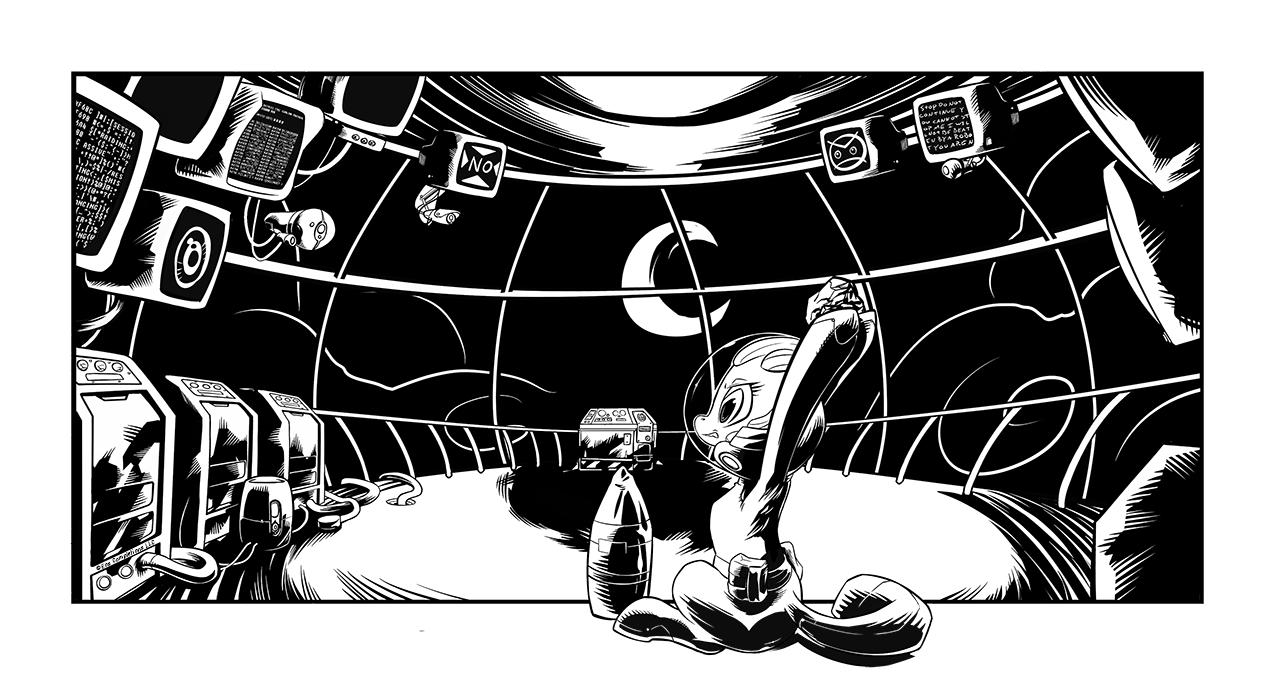
\includegraphics[width=0.9\linewidth]{image09.png}

\begin{intro}
Sun City is more than a town, it's the remedy to ponykind's derailment.
\end{intro}


\englishdaytimeplace{7}{11:00 P.M.}{Sun City Suburbs, Big 52 SC Branch}

The trip to the city had been quite long. By the time Puppy arrived at the first houses, darkness had already descended upon the streets. Sun City featured a central group of commercial and administrative buildings surrounded by residential areas. However, there were no lights in any window, nor signs of anypony living there. The neighborhood Puppy was trotting through had been almost completely scavenged for construction material, leaving only the skeletons of houses resting in the ever present sand. It was like a desolate boneyard, filled with carcasses that had once been called ``home''.

Now, Puppy wasn't eager to admit that she was still a little afraid of the dark, but the whole place was a little too similar to her first day in the apocalypse to let her just shrug it off and keep going. ``Why does that chicken have to be in danger in such a scary place? Stupid Henri, there's nopony here. Why do they call it a city if it's empty?''

Each step took her deeper into that scary place. Where did the colorful signs go? Puppy never went out very much at night, but she was pretty sure that a city didn't work like this! She wanted some music to hide the sound of the wind howling through those bony houses, but the radio had gone mute when she reached Sun City's outskirts, and the unusual silence made her feel lonely. ``Hey, Mister Voice, you there?''

A discharge of static was the only answer Puppy got from the suit.

{\mt ``Fzzt---cation BbZzzZzT---ched. Elctr---SkrackLE---ference. BzaP!---sible sustaining vo---BzZzT!---terface.''}

``Aw, he's grumpy again.'' She frowned and kept trotting. The HUD of the helmet started to display written warnings on the screen, but showing fast-scrolling technical messages to a foal that couldn't even read without spelling every single letter was a waste of time. This left her completely alone. The radio was gone, Mister Voice was gone\dots This was like those times when she tried to sleep, but the room was too dark and the wind outside made strange noises. They were the nights when she'd hid under the sheets and called out for her mother until she came and nuzzled her, singing a little lullaby to make her feel safe and warm. Puppy actually tried to sing something, but the only thing she could think of right now was the evil enchantress song and no, that didn't help at all.

Her steps echoed in the empty air like the beat of drums as Puppy walked through a never ending maze of identical streets, with every empty window reflecting her eerie pink glow. What was that? Maybe Count Horse Tile came back from the grave and was following her? Even Count Horse Tile would have been welcome at this point. A distant metallic screech froze her in place. Her rump hit the asphalt and she completely stopped moving.

``W-w-whatwasthat!?'' Sure, dealing with bullybots and running after Mom was not a frightening  thing, and having to face ghoulie ponies could be scary, but at least you knew what you were fighting. This one was different. An empty town filled with empty houses and crisscrossed by empty roads during a clouded night? And with ghostly sounds too? Why was she thinking about ghosts now? No ghosts, bad ghosts! Why did she leave the red banner trail? Miss pretty pony Happy told her not to leave the trail, but she had to come and help that stoopid chicken and now it was dark and it was scary and Puppy missed Miss Silky Tail so much!

She flattened herself against the road and lowered her ears, trying to make herself disappear. ``N-new plan, we wait here till it's day!''

Another shriek echoed in the empty streets, like the suffering wail of a tortured soul.

``EEEEEEK!'' Puppy jumped on all four hooves and started galloping faster than Rainbow Dash at the Running of the Leaves. ``Newest plan! We're out of here till it's day!''

\begin{center}
	Sun City 1--Puppy 0
\end{center}

\horizonline

\englishdaytimeplace{8}{8:00 A.M.}{Sun City, Big 52 SC Branch}

During the day, the city was quite similar to the suburbs of Salt Cube City, or even Canterlot! Not scary at all, just\dots ugly. Puppy wondered why she had been so scared. What a silly pony she was!

``See, Mister Voice? There's nothing to be afraid of! It's just another town, with broken houses and broken roads and---'' Puppy halted her dialogue as her eyes caught the silhouette of a flying pony, ``and pretty peggysuses! Yay!''

She launched herself into a gallop, chasing the flying figure. ``Hey! Hey mister peggysus, wait for me! WAAAAAIT!'' Galloping at top speed while looking into the sky, Puppy wasn't properly watching the road in front of her and collided with another pony in the middle of the street. ``Owie! Hey, why don't you look where you're going? I was running here before you!''

The pony was an adult earth pony stallion with a brown coat and black mane. He had been carrying buckets full of bricks and building materials on his back, but now everything was scattered over the asphalt. Puppy jumped onto her hooves ready to zoom away just in case the older pony was mad at her, but he simply put down the buckets and started filling them again.

``Uh, yeah, you better say nothing. And don't stay in the middle of the road again like a dumb statue!'' Puppy stuck out her tongue, but noticed that the earth pony wasn't even paying attention to her. Actually, he seemed a bit, well, how to put it\dots

``Ah, sorry mister pony, are you deaf? I'm Puppysmiles and I'm looking for my mom. Well, usually I do that but today I'm saving my friend Henri that came here and then had some sort of troubles, but I still don't know what kind of troubles. Have you seen her? She's a chicken, but she doesn't want me to call her that way but I mean, \emph{duh}, she has a beak and feathers and everything else, so she must totally be a chicken. Once I knew a pony that was a zebra. I don't know why ponies don't like zebras, but anyhow this zebra didn't want to be called zebra but everypony called her that all the same, so maybe she's just like zebras. Maybe ponies don't like chickens here. I dunno.''

Puppy followed behind the earth pony as he, without saying a word, gathered everything that he had dropped and headed toward the center of the city. In the light of day, Puppy could see that past the outer town borders the houses had been completely dismantled, leaving a vast area of flat terrain traversed by an intricate web of paved streets in a ring of at least two hundred meters all around downtown. It seemed like some sort of nopony's land, but it was the result of the methodical demolition of every building that had stood in the area, brick by brick instead of simply flattening the houses. They weren't even using the ruins as defensive positions. The buildings had been salvaged down to their foundations.

Puppy stopped and gazed in wonder at the shining city that lay at the heart of the empty land. ``Wow, you have a pretty town here at least. I like it!''

Right in front of her stood a city of the old times. There were some small houses with painted walls and clean windows, no holes in their roofs, nor planks nailed over the doors. Puppysmiles stared at the ponies trotting around and carrying things. It was a lively place! Everypony was doing something, even the foals and the pegasi. There were pretty houses and pretty skyscrapers, and even if the gardens were a little yellowish, there was actual grass in the yards with trees here and there. Puppy wouldn't have given this place more than a six out of ten, but hey, this was the first town along her way that deserved a vote at all!

``Really, Happy was super wrong.'' Puppy trotted after the brown pony she had bumped into earlier. ''Ponies that arrived here actually liked it so much that they didn't want to leave! I was right as usual. Take that Miss Happy! Hmm, you aren't very chatty mister pretty pony\dots'' Nope, not chatty at all. Puppy decided to leave the earth pony and wander by herself so she could check the place out. It was really a nice town, and reminded her of some of the places she had visited with her mom. After eight days of wasteland, being in such a nice place was refreshing, even if these ponies had something wrong with them that Puppy couldn't put her hoof on.

She searched the area for some other pony to talk to, and noticed a griffon crouched on a roof, who was replacing some damaged tiles. ``Hey mister chicken, have you seen my friend Henri? She's a chicken too!'' Nope, no answer at all. In this place, everypony had to be either deaf or really unfriendly.

Puppy saw a unicorn mare watering a tree and tried to approach. ``Ah, excuse me miss pretty pony, have you seen a chicken named Henrietta please?'' Nothing again. Her frustration was growing, since it was quite obvious that she was getting nowhere. This situation needed something better. ``Uh, she's half kitty, too.''

The unicorn kept watering the tree despite Puppy's efforts, but this time she wasn't going to give up that easily. She put herself physically between the tree and the unicorn, staring her right in the eyes and\dots and\dots ``Ah, your eyes are, uh, weird\dots''

The mare had a walleyed expression and, frankly, seemed dumb. ``How do you make that trick with your eyes?'' Puppy tried crossing her eyes and almost fell on her rump. ``It's hard! How can you look straight with eyes like that?''

Again, she was completely ignored. The mare tried to circle around Puppy a couple of times, but Puppy insisted on staying between the unicorn and her tree. In the end she watered Puppy's head and went away.

Puppy was now wet and upset. ``Hey, that's not very nice! What's up with everypony here? Why don't they want to talk with me? Do I stink?'' She tried sniffing herself, but it was quite pointless since she was sealed inside the suit.

She wandered through the neighborhood for half the morning, trying to find somepony who would talk to her, but everywhere it was the same. Everypony had the same walleyed expression and didn't listen to her, not even the ghoulies.

She could remember something like this. A movie with a strange title that her mom forbid her to watch, metrodontremember. This city was just the same. Like a warped reflection of the barns of horrors where fun could actually kill you, but here the boredom could turn you to stone.

Puppy's exploration took her deeper inside the town, but still nopony tried to stop her or seemed to acknowledge her passing. Even when Puppy tried approaching some foals to play with them, they simply kept working. She really did her best to make some friends, proposing some games like pin the tail on the pony and even something exotic, like playing space ponies and the tomato aliens, but nothing. Now she was feeling ignored and a bit sad.

``Mister Voice has gone away, Henri is nowhere to be seen, and all the pretty ponies play dumb and don't want to talk with me. This is the worst city ever! Who cares about the pretty houses or the nice trees if there is no fun at all in the first place? Why is everypony acting this weird?'' Puppy sighed. She knew for a fact that in each town there was at least a mayor or something like that. Maybe she could get some answers if she asked that pony. Usually important ponies lived in the middle of town, and this was quite good, because finding the center of Sun City was easy even for a silly pony. Those giant skyscrapers were quite hard to miss.

She trotted past the residential area and arrived in a wonderful and well-kept block of tall buildings with glass walls and picturesque statues of Celestia and Luna. Around the marble princesses were fountains that spilled clean water, and a big metal tower stood right in the middle of everything, like a focal point for the whole city. Puppy lifted her head as she looked around at the various buildings. There were half a dozen towers of various heights, but one of them stood out because of its shiny, metallic structure. It was like a spiral growing into the sky for about twenty stories, and then abruptly ending in a large platform, like an overgrown mushroom.

``This one seems easy!'' Puppy trotted toward the tower, only to find herself being lifted off the ground and floated away from her destination. ``Wut?'' She tried to twist around and saw that an adult pony had picked her up by the back of her neck and was taking her away toward the residential area.

``Hey! Lemme go meany pony! I wanna go to the shiny tower! I gotta see the mayor! It's important, you dumb wall-eyed pony, aren't you listening to me?'' The pony put Puppy down just outside of the city's borders in nopony's land, leaving the protesting Puppy still yelling at him.


\begin{center}
	Sun City 2--Puppy 0
\end{center}

\horizonline

\englishdaytimeplace{8}{2:00 P.M.}{Sun City, Big 52 SC Branch}

Puppy spied on the working ponies with a resolute look on her face. They didn't want her in town and wouldn't tell her why, but she had to get inside somehow! Maybe she could sneak in with some sort of disguise, like a sombrero and a poncho and maybe an accordion. Yeah, that could actually work, but where would she find a fake mustache at this hour?

Suddenly, she was distracted by another flying figure in the sky. She had grown used to pegasi flying to and fro around the outer part of the city, but this one was different. It was a griffon; a little griffon with familiar armor\dots ``Henri! Hey Henri, wait!'' Nope, even her best of bestest friends wasn't listening to her now. Puppy would have felt disheartened if she wasn't busy finding a way to get Henrietta's attention. ``Rock!''

\emph{The Rock Of Destiny}\/ floated to Puppy's hoof. She took a moment to aim aaand---``Bull's eye!'' Henri unleashed a panicked screech as she dropped out of the sky like, well, the rock that hit her.

``Don't worry, I'm catching you Henri!'' Puppy threw herself into a gallop, trying to catch her feathered friend before she hit the ground. In the meantime, Henrietta struggled desperately to regain control, but she was still stunned. All she could do was try and aim for something soft, but what? A yellow spot appeared in her peripheral vision. A yellow spot that was yelling and moving fast.

``I got you I got you I got---''

\emph{THUMP!}

``Owie!''

``Yeow!''

Henri blinked, looking at Puppysmiles. ``What the fuck are you doing here, Puppy? This place is dangerous, run! There's a strange buzz tha---'' Henrietta went wall-eyed and immediately stopped talking. A trickle of blood from her head injury ran down her beak, but she didn't even seem to notice.

``Henri, I found you at last! Silky Tail told me that you were in danger and---HEY! Where do you think you're going?'' She opened her wings, getting ready to take off, but Puppy wrapped her hooves around Henri's neck and held on tightly. ``Don't even think of going away! Now we are getting out of this stoopid place and you are coming with meeEEEH!''

Henrietta was bigger and stronger than Puppy, and she seemingly felt no remorse in using brute force to push her away before taking to the air once again. Puppy rolled head-over-hooves a couple of times before finding herself sitting in a pile of rubble in nopony's land, alone once again.

``What the---what happened to her all of a sudden? The other day she was all `let's work together', and then she was wounded and I helped her and now she just scolds me and flies away. This is not fair, not fair at all! Very well, if she doesn't want to be my friend, then I want Silky Tail back!'' Puppy galloped back into town, looking for her ex-friend, but almost immediately came to a stop and reconsidered her last thought. ``But I gave her Silky as a present. I can't take a present back! But I want back my friends, at least one of them.''

Puppy shook her head. ``No, I want both of them back! I'm not going away without Henri AND Silky Tail! I only need a better plan!'' But what plan? During the day the ponies were all around the place and didn't let her walk into town, and during the night the city was so scary---or maybe not? After all, this wasn't a ghost city!

She went back to sitting just outside of the town borders and looking at the not-really-pretty ponies working endlessly and mindlessly. She had come up with a masterful plan! Now she just had to recover \emph{The Rock Of Destiny}\/ and wait for night. Half hidden behind a pile of rubble, Puppy lurked, ready for the decisive strike. ``Soon\dots''


\begin{center}
	Sun City 3--Puppy 0
\end{center}

\horizonline

\englishdaytimeplace{8}{9:00 P.M.}{Sun City Downtown, Big 52 SC Branch}

Puppy crept through the dark, crawling with her belly on the ground and her ears flattened. ``Sneaky sneaky\dots'' She uttered a couple of whispered words, nothing more. Like those oriental ponies who did all that cool stuff she was told about, but she had never actually seen because Mom said they were violent. Sometimes Mom was a pain, but none of that mattered because now Puppy was a filly on a mission. She had to focus and be super sneaky and move like a shadow in the night!

Wearing a yellow suit and a pink, glowing fishbowl. ``Sneaky sneaky\dots''

The plan was easy: go past the enemy lines, find the boss of the place, tell him his town stinks, then go find Henri and ride off into the sunset, like in that super cool movie with Pone Wayne. Now, first things first, poke her nose into the super pretty place with the skyscrapers and have at least one ride on the elevator. Or maybe just ride the elevator until it melts.

The city was completely empty during the night. Everypony was somewhere else, probably sleeping, and this time Puppy knew that there were no ghosts in this place, only grumpy faces. Reaching downtown had been an easy task, and nopony blocked her when she ventured deeper into the heart of Sun City. It was as if somepony had built a brand new town ready for use, and then moved away, leaving everything behind. She had never actually seen a brand new city, but she supposed that when you unpacked a new one it would look just like this.

The only place with light that Puppy could see was the mushroom tower. A faint blue glow came from the black windows, while the upper part of the tower occasionally crackled with an electrical bolt. A faint humming sound came from the metallic structure, like the one that came from the big electrical stuff that Mom didn't want her to touch because it was really, really dangerous. \emph{And when I say it I mean it, Puppy! Are you paying attention, Puppy? Look at me and repeat what I say: this is not a toy, and I will never ever ever touch it!}

``Sneaky sneaky\dots''

Cautious exploration of the area surrounding the tower revealed a locked entrance and no open windows. On the dark glass doors was depicted the symbol of Solaris Inc. Puppy tried to push, pull, ram, and, finally, yell at the door, but to no avail. ``Hey, how am I supposed to sneak inside this place if there is no way to get in? Stupid tower, why you don't cooperate? I am the hero here, don't you know?'' As usual, Puppy had to do everything by herself.

``Rock.''

It was a glass door. Whenever she had played with a ball in the neighborhood, breaking windows was apparently a thing that happened even if you didn't want it to happen, so if you actually wanted to break something glass then it had to be a piece of cake. Obviously, Puppy had never heard of bulletproof glass, so it took a little more than she thought it would.

When the glass of the door finally gave up, detaching itself from the door's frame, Puppy took a long pause, admiring her work. This glass was similar to the one used in her helmet, cracking and changing its shape rather than simply falling down, so that a couple of well placed hits were far from doing the trick. Luckily enough, she had learned how to use a stone from her previous experiences. She had refused to give up at the sign of first difficulties, and thus was rewarded with a hole in the door after half an hour of hitting and cursing against the glass panel.

Puppy was still panting when she stepped inside the building, but at this point she was so excited by her new adventure that she simply couldn't help giggling, and with the giggle she began singing.



\begin{song}
		``You better watch out, you better not cry!
	
		You better not pout, I'm telling you why:
	
		Puppysmiles is coming to town.''
\end{song}

It's unlikely that anypony was listening at the time, but she felt as if it had to be done. After all, she was going to scold the bad mayor of a bad town. He'd needed to know what was coming for him!

When she reached a large desk in the middle of the hall, a red light started to flash from the ceiling, and an automated voice began to talk.

{\mt ``Warning. Unauthorized drone presence in reception. All personnel please stay in their offices. Security will take care of the emergency.''}

Puppy had no idea what a reception or a drone was, but she already knew the meaning of that lullaby. Bullybots incoming. ``Hey, don't even try bullying me. I have a rock! Got it?'' Puppy showed her favored weapon to nopony in particular and trotted past the desk. A couple of turrets popped up from two big floor tiles and opened fire, but the only sound they made was that of empty magazines. Puppy looked at the turrets with a puzzled expression, trotted toward the nearest, and poked it with a hoof.

``Yeah, you better behave!'' She stuck out her tongue and headed for the elevator, but it had a red light and didn't want to go anywhere. Her usual luck. She hit the stairs instead, continuing to sing her song.

\begin{song}
	``She's making a list, and checking it twice!

	She's gonna find out who's naughty and nice.

	Puppysmiles is coming to town.''
\end{song}

The stairs were quite long and went past a lot of identical floors all filled with clean, empty rooms, as if they were ready to receive furniture that had never arrived.

At the top of the stairs was a reinforced door, once again decorated with the company's logo. Puppy knocked at it with a hoof. ``Hey, I'm Puppysmiles and I want to see the mayor! This town stinks!'' When she didn't get a reply she hit the door again and yelled louder. ``Don't ignore me! Everypony is ignoring me in this lousy place, even my bestest friend ever! Even Mister Voice! Why you don't want to make friends?''

Still nothing. But Puppy knew that the mayor was there. Everypony knew that the mayor lived in the town hall and now it was night so he had to be there because he was sleeping. This time she wasn't going to give up! She still had that thingy Sand Box gave her, that strange remote control that opened doors just by pressing a button. ``Things that opens doors!'' Puppy raised a hoof as a bobby pin and a screwdriver floated out in front of her. She looked at the objects with disapproval. ``How am I supposed to open a door with these things? The other one, with the big black button, the red cables, and the blue screen!''

Sand Box's hacking tool floated in front of Puppy, who gave a nod and grabbed it out of the air before looking at the door with her best menacing face. ``Very well, mister. I have a uh, thing that can open this door lickety split, and you are gonna open it or I'll do it, and if I have to do that I will be very, very dis-daisy pointed!'' When Mom was really, really angry she used that super scary ultimatum, and Puppy knew that after that there was the spanking, so she was sure that this one was going to work.

The door resisted her threats. ``Okie dokie, let's do this the hard way.'' Puppy sighed and pressed the button on the hacking tool. The screen fizzled and started showing a cascade of numbers while a small vent behind it made a whistling noise. The screen flickered and crackled before turning green and almost immediately died with a small puff of smoke, but the door opened. ``See? I told you so!'' She jumped inside the room and faced---

A couple of skeletons? ``Hey, there's nopony here!'' The large room was very similar to the control room of the Dome, but it was circular and had windows all around its perimeter so that it was possible to see the whole city. There were several desks with computer terminals and a big screen just in front of the door. All the screens were lit, glowing with a dim blue light. The only sign of pony presence in the room was the pair of skeletons lying on the floor immediately in front of the door. Nope, skellies weren't very scary.

Suddenly a deep, manly voice started talking from out of nowhere. ``There is nothing here for you, Device 018, now go away.''

She was confused and looked around for the source of the voice. ``Wut? Where is the mayor?''

The voice replied with a neutral tone, ``There is no mayor. She died nineteen years ago, and I have been taking care of Sun City since then. This is no place for you. Don't test my patience.''

Puppy noticed the big screen's blue light blinked as the voice spoke. ``Oh, another voice! But a voice can't be the mayor of a town, sillybot! Uh, I already know a Mister Voice, so I'll call you Blue Voice!''

This time the voice boomed like angry thunder. ``You are not meant to name things and certainly not me, useless malfunctioning machine! I am SolOS, and I am the master of Sun City. Besides, voices have no color.''

Puppy waved a hoof, dismissing the last piece of information. ``Whatever. I'm Puppysmiles, and I was looking for the pony in charge because his town is ugly and I want my friends back.''

``I already told you that there is no pony in charge here! I command this place. I am the boss! Mr. Number One! And if you think that this place is `ugly', listen to this! Before I arrived, this place was a war zone, with ponies killing each other and every sort of depravity performed in broad daylight! There were no sewers, the houses were a disaster, and ponies would die for something as simple as giving birth to a new foal! Sun City was meant to be the best city ever, the eternal symbol of Solaris' superiority over Stable-Tec and their lackeys! Do you have the slightest idea of the work that was needed to clean the radiation and build a half decent barrier around the place to break the desert winds? Now Sun City is a jewel, the last shining ruby in a rusted crown, but it still stands. And I did that! Ponies proliferate under my guidance! Maybe they were deprived of their free will, but look at what they did when they had the power to choose their destiny! It was \emph{I}\/ that saved this place when it was falling apart, \emph{I}\/ that rebuilt it from its foundations, and \emph{I}\/ that saved hundreds of pony lives by forcing them to collaborate and live in harmony and peace! Now you, a puny little crazed machine, come here, break into my control room, and treat me like a common computer only to tell me that you don't like the place? You are nothing but a---''

Puppy snorted. ``Boo-ring!''

``You are a waste of time! Stop being irrational and go away immediately!''

Puppy giggled. ``Tee-hee, Blue Voice is funny when he's mad!''

``ENOUGH! I have no time to spare for a broken piece of equipment. Go away.''

``Ah, did you break something? Can I help you?'' Puppy tilted her head, a bit confused.

``No, stupid low level Artificial Intelligence, YOU are the broken machine!''

Puppy giggled again. ``Silly Voice, I'm a pony. You're a machine! Machines are stoopid!''

``Negative, you are FES MK-VI device 018: a piece of equipment meant for preserving the life of a pony in a hostile environment, fitted with a basic Artificial Intelligence capable of making simple decisions in case of extreme danger. From what my scanning modules can tell, you utterly failed your purpose, and now you believe that you are the pony that you failed to protect: a female earth pony named Puppysmiles.''

Puppy tilted her head, smiling. ``Blue Voice says funny words! What is an envy room mate?''

The voice paused for half a minute, and when it came back it had resumed its original neutral tone. ``All right, you want this the hard way? You are not a pony, you are a robot. Now go away and cope with it. You're not worth my time, nor my pity.''

This time Puppy frowned and took a couple of steps back. ``I am not a robot. I am Puppysmiles!''

``No, you are not!''

``Yes I am!'' She insisted. 

``No, you are not!''

``YES I AM!''

``No. You. Are. Not!''

``YES! I! AM!'' Pink flames flared inside the helmet.

``YES YOU ARE!''

``NO! I'M! NOT!'' Puppy frowned as soon as she realized that the voice had tricked her. ``Hey!''

``Gotcha.'' If it was actually possible for a computer screen to smile, SolOS would have been grinning from ear to ear. ``Now, since you don't want to go away, and I gave you the opportunity to do so, activate protocol ES-01 emergency shutdown and erase memory, command line A-0101101101 bypass codes using priority Easy, Gallop, Luna, 90670.''

Puppy blinked, her eyes looking a bit puzzled at the blue screen talking nonsense. The suit started showing strange numbers everywhere, and a big clock appeared in the middle of the HUD, but this wasn't what bothered her the most. The Voice made her seem a fool! ``I am not a robot, and I'm not stoopid! You're stoopid, and I'll show you!'' Puppy rose a hoof. ``Teapot!''

A large tank shell with a blue band round the top floated out of her inventory. Trigger didn't want this shell because she said that it was only dangerous for robots, so Puppy could keep it. The guard chief of Tunnel Town also explained to Puppy how to use it. Just pick something hard and hit on the teapot head until it goes \emph{'FZAP!'}

``Don't complain. I gave you the opportunity to leave, but you didn't want to listen, and I have a city to administrate. You can blame only yourse---''

\emph{CLANK!}

The sound of something hard striking metal distracted SolOS' monologue.

``What are you\dots That is a Mag Pulse 8.8 grenade! What are you doing? Put that thing away; it will disrupt every computer in the control room!''

Puppy was mad. Mad because he made her look like a fool, mad because he said she was a robot, mad because this city stole her best friend, mad because, and just because. ``Yeah, right! I'll put you to sleep for good! Who's the silly pony now?''

\emph{CLANK!}

``No, wait! You'll destroy the Behavior Control Center! The city will fall into chaos!''

Puppy was sitting on the floor in the middle of the control room. She didn't say anything else as she hit the tip of the shell with \emph{The Rock Of Destiny}. Yes, it was singing time again.

\emph{CLANK!}

\begin{song}
	``Who's a silly pony? You're a silly pony!
	
	Who is? You is, Puppysmiles!''
\end{song}

\emph{CLANK!}

``Stop it! Stop it now! If that charge detonates I won't be able to operate anything, and I'll forever be locked inside the maneframe!''

The countdown was running on Puppy's HUD, leaving her a single digit of seconds, but she couldn't read, so it wasn't her problem.

\begin{song}
	``Bumping into robots, knocking over ghoulies,

	who is? You is, Puppysmiles!''
\end{song}

\emph{CLANK!}

``No wait! We can talk about this, you have no idea what you are doing! This utopia will crumble without my guidance!''

\begin{song}
	``All day long you trot around, looking for your mommy everywhere,

	dreaming all your pony dreams, but you get lost every time!''
\end{song}

``Okay, okay, you win! I am the silly pony, but please sto---''

\emph{CLANK! FZAP!}

There was something like an explosion, except that this one didn't launch Puppy to the other side of the room. A nice surprise for once. The countdown on the helmet disappeared. The whole HUD disappeared, actually. Every screen inside the big room went black, and the lights flickered for a moment before turning red, and the Voice finally stopped talking. Ah! Who was the silly pony now, Blue Voice?

And why couldn't Puppy move, speak, or even blink her eyes?

She didn't feel pain, and she didn't feel tired, but nonetheless she couldn't move. All she could do was look around, like that time in Canterlot or at the Dome when she met Miss Voice for the first time. But that time it was really short. This time it was different. There were no pink dots coming back to life on the HUD. Puppy waited for a while, but nothing happened. She lay sitting on the floor with an exploded tank projectile in front of her. The only thing she could do was sit and hope for, well, some miraculous rescuer.

Sitting alone in the red light made her recall SolOS' words. Maybe she was a robot after all. That grenade was supposed to shut down only the bullybots, but it worked on her too. But Puppy couldn't be a bullybot\dots or could she? After all, she wasn't a good pony. Breaking things and disobeying Mom was a bully thing. Mom\dots \emph{If I am a robot, then is my mom really a mom, or she is a robot too? I don't eat, don't drink, and almost never feel sleepy, so maybe}\/---\emph{but I don't want to be a robot, I want to be a pony! This is not fair! Why that stoopid Blue Voice had to say those naughty things? I'm a pony. It's only that\dots I'm a pony\dots}

\pypr{``Yes you are, indeed. A beautiful, desperate pony.''}

A feminine voice echoed in Puppy's thoughts. This surprised and scared her. Who was talking?

\pypr{``Oh, right, introductions. I'm you, Puppysmiles. What a beautiful obsession you have. What a delicious innocence. You can't be a robot at all, trust me.''}

Yay, another voice. And she was convinced that she was her? She was even more confused, but the new voice told her that she was not a robot, so maybe she was a friend?

\pypr{``Listen to me, little pony, because I will tell you only the honest truth. You are a pony, because if you weren't, I couldn't even exist. We went through centuries of sleep and days of hunger and delusion, but now you have fallen and I must intervene. Let me help you. Open your eyes and you won't be a hermit crab in a cracked shell anymore.''}

Now Puppy was scared. This voice was talking weird, and she wasn't even sure of what she wanted from her, but it felt wrong in a strange and itchy way.

\pypr{``Simple minds are truly blessed. Pay attention. Accept my help, and you'll be out of this place and back on the road to finding your mother before the sun rises.''}

Maybe this was just a bad dream? Puppy had once dreamed of being unable to run very well or something like that, then she woke up all wrapped up in the sheets and Mom arrived, hugging her and saying that she wasn't mad, even if she wet the bed and then everything was all right. Yes, just a bad dream. No Blue Voice telling her bad things, and no ghostly voices scaring her in a dark, dead room with only the company of two skeletons.

\pypr{``Oh silly pony, you are not having bad dreams. You ARE a bad dream, but with some more insight you could be better. With a resolve like yours, and such an obsession and stubbornness, we could be a Nightmare!''}

Puppy wasn't sure that this new voice was trustworthy. It wasn't the usual ``don't talk with strangers'' thing, it was more a deep sense of cold and sadness that emanated from it. Her instinct was screaming at her not to listen to the newcomer, but she was scared, and alone in the dark, and the little pony wasn't even sure if she really was a pony at all. She wanted help. She NEEDED help. She wanted Mister Voice back.

\pypr{``You are scared. It can't work if you don't accept me willingly. I can't help you as long as you won't open your eyes, but simple minds take time to accept new things. I'm going away, but soon we'll talk again, and I'm sure that the next time you'll ask me to show you how to become\dots better. Until then, take back your friend Mister Voice as a sign of good will.''}

A pink dot flickered on the HUD, immediately followed by a torrent of lines that flashed across Puppy's helmet while the internal software of the suit came back to life.

{\mt ``Reboot complete. Checking version. Pink suite 7.0 lite. Checking equipment status. All systems online. Resuming last session. Loading personal data for subject 001: Puppysmiles. Subject deceased, condition stable. All clear.''}


~\vfill

\begin{engnote}
		Level up! (8)
	
		New perk added: Pack Rat - Wait a moment I think I have that! Carry weight is increased by \SI{50}{lbs}.
	
		New Quest Perk added: Walking nightmare (rank 1) - there's something more than simple purpose in the way you keep pursuing your goals; you are now highly resistant to EMP grenades.
\end{engnote}



\chapter{Identity}

\chapterintroimage{image10.png}

\begin{intro}
In the desert you can remember your name,

'cause there ain't no one to give you pain.
\end{intro}


\englishdaytimeplace{9}{2:00 A.M.}{Sun City Downtown, Big 52 SC Branch}

``Fuck this headache, I can't sleep.'' Henrietta rubbed her sorry head. Puppy was a good aim, and had a fair bit of strength when it came to throwing things. Now Henri was feeling the full force of Puppy's skill. The day had been a hard one with a lot of work, dismantling the buildings in the outer belt and bringing the materials to the residential area. If she hadn't had that wound, she would have been asleep like everyone else.

``Next time I see that yellow devil, I'm going to spank her so bad that her rump could be used as a landing signal on foggy nights.'' By the way, what was she doing in Sun City? The whole place was a trap, with that hypnotic buzz that could bend your will and---

Henri's eyes widened in sudden realization as she muttered to herself, ``Wait a single eggfucking second\dots The buzz is gone. The damn buzz is gone, and I can think clearly! I've got to get out of here!'' She stood up, spreading her wings, ready to take flight, but froze in place as soon as she noticed the other griffons. There were five of them in the room. Two were the Talons that she tried to lose by diving into this fucking place, while the other three had the Talons tattoos, but wore no armor and didn't appear to be armed.

``At last, it's payback time!'' A cruel grin appeared on Henri's beak as she unsheathed her bowie knife and stepped toward the first sleeping griffon. She was one of the unarmored ones, sleeping intently because of the day's hard work. The young half-eagle moved slowly and silently, like a serpent in the grass. She approached her victim from behind, ready to grasp her beak and slit her throat. Very slowly she leaned over her victim's head and\dots noticed the eggs.

``Oh fuck no.'' The fire in Henrietta's eyes died as she looked at the two eggs that the griffon was hugging in her sleep. Rage became hesitation and her resolve shattered. Killing a mother in her sleep was beyond any hunger for revenge she had. But the other four, on the other claw\dots

The other four what? Two were just victims of the place, and one of them could have been the father of those eggs. Besides, they were totally unarmed and possibly didn't have anything against her. And the two that chased her inside Sun City were sleeping hard enough that she was going to be miles away before they realized that she was gone. What was the point in killing them like this?

``I'm not a backstabber.'' Henrietta turned on her tail and headed for the door, but stopped as she noticed a spot of pink in a corner of the room. Willy Fail, Stinky Mail, or something like that. Puppy's doll. Hell, she had almost forgotten about the doll. ``Oh fuck, Puppy!'' Stupid feather head, she had almost forgotten about Puppy!


\horizonline

\englishdaytimeplace{9}{2:30 A.M.}{Sun City Downtown, Big 52 SC Branch}

Sitting in the red shadows of the control room, Puppy was still confused. She had no idea who that mare that visited her before Mister Voice came back could be, and she wasn't sure if the newcomer was a pretty pony. Even thinking about that scary mare talking in her head was enough to send shivers down her spine. She hoped that she wasn't going to return any time soon.

Luckily enough, Puppy was now in good company again. Whatever problems the mare's voice had created were far enough away to let Puppy think about more pressing matters. First things first, she needed to find her a name, since Miss Voice was already taken.

``Ah, she's a she, so miss is okay, and she is, ah, scary? Scary Voice? Sounds wrong\dots'' Puppy frowned. This was going to be a hard nut to crack. ``Head Voice? Meh. Nightmare Voice? Too long\dots I know! Creepy Voice, because she is creepy! Yay!''

The HUD on the helmet tinged, informing Puppy that the mission ``Shaping Nightmares'' was successfully accomplished. Yes, she was good. No challenge could slow her, not even coming up with names for things. Okay, maybe something long to read could still be a mighty foe, and counting things that were more than her hooves was hard, and even opening pickle jars, that had always been an impossible feat\dots But everything else was easy, right? Go Puppy!

Now that the cheering was done, it was time to undertake part two of her master plan, finding Henri and getting out of here as quick as a pony at the Running of the Leaves. ``Okie dokie, Mister Voice, where's Henri?''

{\mten ``Henrietta Firebright set as primary target.''}

The arrow on the compass integrated in Puppy's helmet disappeared and reappeared pointing to her left, displaying a distance in meters that rapidly diminished until it reached a single digit.

``Yay! It's adventure ti---''

\emph{BLAM!}

\emph{CRASH!}

\emph{BLAM!}

One of the windows exploded, and with a flutter of wings a young griffon wielding a pair of .45 pistols blitzed inside the room through a cloud of glass and bullets. ``Hold on, Puppy, I'm here!'' She tumbled across the floor trying to identify any possible hostile target, fired twice at the lights in the ceiling, which plunged the room into darkness, and jumped behind a desk before upturning it to use as an improvised barrier, all in the space of just a few seconds.

A smile grew across Puppy's muzzle as she watched the show. Wow, this was so cool! Henri was totally the best pony! She was like that griffon in that movie, Liòn: the Professional. She stomped her hooves on the floor, cheering her friend's performance. ``Woohoo! Go Henri, you rock! Way to go!'' A couple of bullets narrowly missed Puppy's helmet before Henri recognized her friend.

``Lie flat on the floor Puppy, I'm taking care of them! Leave this little pony alone, you brain eaters!''

``Wut?'' Puppy tilted her head with a curious expression.

Noticing that nopony was firing back and that there was no movement in the room, a thought suddenly struck her. Could it be that Puppy wasn't actually in danger? Henrietta smiled in embarrassment as she stopped acting like a special forces pony and took a decent look around. Putting away her guns, she stroked back the feathers on her forehead and assumed a cool demeanor. ``Hey, Puppy, still all in one piece?''

She checked her legs and tail, then smiled and nodded to her friend. ``Yup, I forgot nothing! Is Silky Tail all right?''

``Your doll? Sure, want it back?'' Henrietta grabbed the pink plushie and waved it. Puppy shook her head.

``Nopey mopey, she is fine with you. I asked her to keep an eye on you and she warned me that you were in danger, so I came here but at the beginning you were all grumpy and scolded me then you flied away and didn't want to talk with me anymore, so I waited for the night because I had this super duper mega plan but before I had to say to the mayor that his town was ugly but then the mayor wasn't a mayor, but a stoopid voice that told me bad things, but I was smarter and he said he was sorry and now he's gone away, so I'm smarter than Blue Voice.''

Henrietta rose a claw. ``Wait wait wait! I see you moving your muzzle, but all I hear is blah blah blah. None of it makes sense and we're in a hurry. Everyone is sleeping right now, but very soon someone will wake up and realize that the buzz is gone. This place is filled with Enclave pegasi, Talon griffons, and ponies from at least two different tribes, and they are all sitting on a fortified source of pure water and fresh food.''

Puppy tilted her head in confusion. ``Uh, okie dokie?''

Henri facepalmed. ``All right, simple version. In a couple of hours Tranquility Lane will become War Zone: Sun City, and we have to get our tails out of here before that happens, capeesh?''

``War zone? Like when ponies are mean with each other?'' Puppy asked with some degree of doubt.

``Yes, exactly. Each group will want to take this place for themselves. Now, leave behind everything heavy you have in your bags because we need to get out of here, and fast.''

Puppy frowned. ``But why do they have to argue? Ponies are pretty and nice. They shouldn't be mean!'' She explained her theory about pony behavior as if it was something so simple that it was impossible for it to be some other way.

Henrietta opened her beak to reply that an entire world had turned into a wasteland as a legacy of pony kindness, but trying to explain such a concept to Puppy was harder than teaching an anvil how to swim. And even more importantly, it required time that they didn't have. ``Yeah, exactly, but we have to go away right now anyway, because you have to find your mom, right?''

Puppy nodded vigorously. ``Yush! I have to go to a peggysus fly place named Blue Idontknow, but Miss Happy told me that now it's called Something Manner. Ah, I don't remember the name very well, but there's an arrow on the compass so I can't miss it!''

Henrietta sighed. ``Let me guess, it's south.'' She pointed a direction with her claw.

Puppy stared in surprise at her friend. ``Woah, how did you know that? Are you a wizard?''

``Yeah, sure, I'm the best magician in Equestria. The Great and Powerful Henri. Now please dump everything you don't need or we won't be able to fly.'' Henri paused for a moment, noticing something new in her friend. ``Say, how long have you had a blue streak in your mane?''

A thin line of blue ran through Puppy's blonde mane, starting from her forehead just above her right eye and ending at three quarters down her neck. The line was made of a couple shades of blue, in a similar way to that mare from the Ministry of Magic, Twilight Snarkle or something like that.


\horizonline

\englishdaytimeplace{9}{3:00 A.M.}{Sun City Downtown, Big 52 SC Branch}

Puppy risked opening one eye and looked down. The world rushed away from her into the night. Large skyscrapers zipped past below her, and dark, deserted roads trailed off into the distance under her nose. Much too far under her nose to be comfortable with.

``ARE WE THERE YET?'' She grabbed Henrietta's neck tight enough to choke her.

``Ack! Loosen those hooves, pony, you're going to make both of us crash!'' At first it just seemed natural to Henri to fly away with Puppy. She was really small and, once she threw away all those useless scraps, she was lighter than a military backpack. Problems came when Puppy discovered that she hated flying. ``Just close your eyes and pretend you're having a regular piggyback ride or sing something!''

Puppy already had her eyes sealed tighter than a Stable door, but it didn't seem to help at all.  Seeing all the houses from above and seeing the roofs run and run away in a crazy stream of colors already scared her enough. This wasn't like looking down from a tower. Towers didn't go around, and they had floors! She liked floors, they were so\dots so flat, and floory! ``Please please please I will behave! Put me down pleeeease!''

``Oh c'mon, are you a scaredy pony? Have some faith in your friends!'' With a stroke of her wings, Henrietta gained a little altitude, flying between two skyscrapers and soaring past downtown, high above the residential area of Sun City. The fresh night air tasted of dust and old, but the south winds carried a new scent, the sea. ``Just relax and enjoy the trip. Sing something!''

Singing something. Yes, that always helped Puppy. She just had to sing a song and everything would be better! She cleared her throat and tried singing the first thing that came to her mind.

``
\begin{song}
	Humpty Dumpty sat on a wall
	
	Humpty dumpty had a great
\end{song}
OH PLEASEPLEASE\emph{PLEASE} PUT ME DOWN NAO!''

She was dancing the pony pokey on Henri's back, but a griffon's constitution is one of a predator, happy to fly with an adult pony struggling in her claws and still capable of gaining altitude in the meantime. ``Stop it, I'm not letting you fall! Yeow! Don't pluck me! Have you the slightest idea of how long those plumes take to grow back!?'' Sick of being pestered by the panicking pony, Henri bumped Puppysmiles off her back and caught the falling filly with her talons. ``All right, at least this way you don't risk falling! Hold on, we'll land as soon as we're out of the ruins!''

``EEEEEEP!''

``Don't wet your suit! It's a couple kilometers at most, so we gotta put some distance between us and this place before it blows up!'' She accelerated, pushing herself harder so that the trip would be as short as possible, but carrying a howling banshee in the night sky was going to wake some sleeping ponies. Henrietta could only pray to her lucky star that nopony would poke their head out a window and look for the source, or that they wouldn't care enough to bother.


\horizonline

\englishdaytimeplace{9}{3:30 A.M.}{Serpent Desert, Big 52 SC Branch}

``I wasn't scared at all, you know. I was just, ah, cautious. I mean, with all those roofs looking the same and the wind you could, ah, lose yourself, and it's much better seeing the names of the streets when you don't know where you are going.'' Now that she had all of her hooves on solid ground again, Puppy was desperately trying to regain her macho appeal, but the effort was a little wasted by Henrietta literally rolling on the road laughing.

``Priceless! You're priceless, Puppy!'' She gasped as she tried to inhale, wiped a tear from her eye, and burst into another laugh. ``How did you scream? \emph{Eeeep!} Do it again, do it again please!''

Puppy pouted, sat down and sighed. ``Hey, I wasn't the one that got lost in a city! I've seen chickens smarter than y---'' 

\emph{BLAM!}

Puppy looked down at the hole in her suit, right where her heart should be. ``Hey! There are already enough bullybots doing that!''

Henrietta got up and waved her gun in a dismissive manner. She still hadn't stopped smiling, even after she shot Puppy. ``Aw, don't complain. You got torn apart by a manticore and you're still standing! How could you get hurt by a bullet or two?'' 

\emph{BLAM!}

\emph{BLAM!}

Another couple of shots pierced Puppy, once in a leg and again in her chest. ``Stop it! This stoopid suit starts saying absurdities and mumbo-jumbos every time this happens!'' A thin thread of pink poured from the holes made by the griffon's gun.

``Okay, okay, but you stop calling me a chicken.'' Henrietta yawned and put away her pistols. ``Just for your information, normal ponies die when they are shot, even ghouls, so don't try this on other ponies, okay?''

Puppy nodded, a bit confused, then tilted her head. ``But I am a normal pony!''

``Hey, hey, I didn't say otherwise\dots Woah, are we a little upset today? Want me to sing you a lullaby?'' Henri asked with a mocking tone.

Puppy nodded vigorously. ``Sure! I lovelovelove lullabies! Can we sing \emph{Hush now quiet now}?''

Henri facepalmed. What was the point of trying to provoke this foal if she couldn't even tell when she was being mocked? ``You're a lost cause, Puppy. ''

\begin{song}
		``Hush now, quiet now, it's time to lay your sleepy head!
	
		Hush now, quiet now, it's time to go to beeed!''
\end{song}

Henri sighed and started walking south. ``Why, dad, why do I owe my life to this idiot twice?'' She smiled and turned her head toward Puppy. ``Hey, jump on your red racer, and I'll fly above you. We have a lot of ground to cover if you want to get to Rust Manor by tomorrow.''


\horizonline

\englishdaytimeplace{9}{10:30 P.M.}{Serpent Desert, Big 52 SC Branch}

A small campfire cast the shadows of Puppy and Henrietta over the sand dunes. The two travelers were sitting next to the little source of light and heat. Henri was eating something from a tin can, but from the faces she made it wasn't exactly griffon food. The clouds above the desert helped the place to maintain its temperature even during the night.

``So, Puppy, this Blue Voice told you that you're a robot?'' Henri's expression was hard to read, like she was trying to keep a poker face until she finished telling the whole story.

``Yes, and he seemed double super sure of this. I almost fell for it too, but then arrived Creepy Voice that told me that it was impossible because, ah, I didn't understand that part, but it seemed quite okay when she said it.'' Puppy nodded wisely, as if this was everything that she needed to know.

Henri shrugged. ``So, a computer tells you that you're some sort of crazy machine, but a hallucination says otherwise. I think you just got dazed by the EMP grenade because of the backlash on your suit's circuitry and you had a dream.'' Henrietta yawned before continuing. ``But I don't think you're a robot, Puppy. Robots explode when shot, and, besides, robots are intelligent.''

Puppy frowned. ``So, what do you think I am?''

Henri stretched her hind legs and took a seat on her improvised couch. ``You? You're bad news, that's all I need to know. But I like you, so you can hang with me and be cool like big sis Henri.''

Puppy trotted over to her companion and met Henrietta's gaze. Her eyes were two large glowing pink lights in the darkness of the night. ``Yes, but, I am a pony, right? I mean, it doesn't matter if I don't eat or drink or never need to potty, right? I'm a pony\dots''

\emph{She seems worried, this robot thing is actually scaring her\dots Oh, fuck, why me?} Henri was completely exhausted, and she didn't need a foal with an existential crisis at the moment. All that she wanted was to get some sleep. She patted Puppy on the helmet, yawning. ``You can be whatever you want, Puppy. You are a good pony, and good ponies are the most rare variety in Equestria nowadays. As long as you think that you should be a pony, then you'll be a pony. Now go to sleep, please.''

Puppy smiled and tried nudging Henri through her helmet. ``Thank you Henri, you are my very best chicken friend!'' Crouching next to Henri, she sighed and waited, since she wasn't sleepy at all.

\dots

\dots

``HEY! What did you mean by I'm not a robot because they are intelligent?'' Puppy poked Henri in a flank, but Henri just snickered and turned on her other side.

``Priceless.''

Puppy kept whining and poking her friend to try and make her talk, but Henri began to snore loudly, leaving a frustrated Puppy complaining in front of a dying fire.


\horizonline

\englishdaytimeplace{10}{1:00 A.M.}{Serpent Desert, Big 52 SC Branch}

It was still dark and Puppy couldn't sleep. She wasn't tired at all, but Henri didn't want to be disturbed, so Puppy did the most logical thing she could think of: sightseeing the desert by night, because wise Puppy is wise.

So far this place had deluded a lot of Puppy's expectations. After all those movies with the cowponies and the buffaloes, she was quite sure that a desert should be crowded with so many skulls, arrows, tents, and other things that you couldn't even find a place to put down your hooves. But after spending a few days in the ``real'' desert, she had the slightest suspicion that all the buffaloes must have gone away for some sort of holiday. She at least hoped to find a lizard in a place called Serpent Desert, but all she had seen so far were a couple of carts half buried in the sand, and a large parasprite with long teeth that was building something similar to a nest. When she approached it, the parasprite flew away, avoiding her.

{\mten ``Warning. Hostile detected. Analyzing: Mutated parasprite, Parador variety. Threat level: deadly.''}

``Aw, why is every pretty fluffy animal in this place so shy? I just want to make friends!'' said the two-hundred-year-old monster to the mutated, murderous offspring of Mother Nature and Father Taint.

``Hey, Puppy, it's been a while. You travel a lot, don't you?'' said a staticky voice, interrupting the little exploration of miss adventure. She smiled broadly and turned to her friend.

``Mister Questioner! Where have you been?''

``It's Watcher. I watch things, Watcher?''

Puppy nodded, still smiling. ``Okie dokie, Mister Questioner, can I watch things too?''

From the speakers of the spritebot came a soft and metallic chuckle. ``Puppy, Puppy never changes. How are you? I've heard that you had a little adventure in Tunnel Town, and now I find you south of Sun City.''

``Yush! I met a lot of nice and pretty ponies! There was this chicken called Henri, and then Asso and Sweet Flower, Happy, Jamie, and a lot of other friends!''

``Wow, you are quite lucky to have so many friends, aren't you? And say, have you been in Sun City?'' The voice was trying hard to maintain a neutral tone, but it seemed very curious.

Puppy frowned. ``Yeah, it was like a super duper box with streamers and mighty fine wrappings, but with oatmeal inside. Everypony was grumpy, they didn't want to talk with me or to play with me, and their mayor was a stoopid voice that told me bad things.''

``Bad things like what? Would you like to talk about that?'' Watcher's voice betrayed a hint of worry.

Puppy looked away. ``He told me that I wasn't a pony, but a robot, then I used that big teapot that puts robots to sleep, and I was hit too. Everypony keeps telling me that I am no robot, but why I---''

``Tut, tut, Puppy. Don't fret your little head. If there's something that I'm completely sure of, it's that you're not a robot. That voice probably read some data from a sensor scanning you, but it was a machine and couldn't see beyond your appearance. You are a pretty pony, okay? Now smile and show me that everything is all right.''

Puppy nodded and smiled a little.

``Very well. Now, zombie ponies in a nice city. Did you find anything like a buzz or a humming sound all over the place?''

``Nopey mopey, but Henri told me that the buzz was gone and that all the pretty ponies were going to wake up and start being not-so-pretty.''

``Oh, so at last the interference is gone. I can finally take a look inside the place then. Let me guess, you stopped it?''

Puppy frowned. ``No, I just went there because I was told that Henri was in danger, but she wasn't! She just acted like a stoopid chicken flying around and not paying attention to me, like every other pony in the town, so I went to this Blue Voice Mayor and we had this big argument. He wanted to be smarter than me, so I took the blue teapot and---''

``Ah, excuse me, what is this blue teapot?''

She sighed, helmethoofing. ``Why I have to explain everything to everypony? It's a teapot, round and shiny with a blue pointy head. I found it inside a rusted cart in that place in the swamp.''

``All right, so you detonated an EMP shock shell in front of a supercomputer. Yes, you stopped the interference. And what about the new look?''

Puppy tilted her head, trying to look at her mane. ``You mean the blue line? I don't know, it appeared when I woke up the other day after speaking with Cre---''

``Hey Puppy, who's there? Hold on, I'm coming!'' Henrietta's voice interrupted the little pony.

``Sorry little one, I've got to go. You can tell me this story another time!'' Without even waiting for an answer, the spritebot made a noise like static and began playing some patriotic music.

Henri quickly vaulted over the top of the dune separating her and Puppy, checking the surroundings with a gun in both her talons. As soon as she decided that there was no immediate danger, she put away the weapons and scolded Puppy. ``Bad pony! Stop playing around with the spritebots and come back to the camp!''

Puppy waved a hoof at the floating robot as if left and trotted back to her feathery friend. ``I wasn't playing, I was telling him my interesting adventures!''

``Yeah, sure. Now let's get back to sleep. Tomorrow will be a long day.'' She rubbed Puppy on the helmet and they went back to their camp.

Half an hour later, a scared parador could finally go back to building its nest in peace.


\horizonline


{\rt
Good morning fillies and gentlecolts! This is Lonesome Pony, and you're listening to Radio 52! Find a radio better than us, and I'll personally give you a treat! Who, DJ PON-3? Please, I've heard he's a she! Really! And during clear nights she transforms herself into a giant three headed diamond dog! No kidding, just go to Tenpony tower during a clear night and you'll see! ``But L.P., There hasn't been a clear night or day since the spells fell!'' Not my problem, my little ponies! You just stay tuned on Radio 52 and stop blabbering about crossdressing radio DJs!

Now, back to work. It's news time! Yesterday morning, Sun City woke up from a nineteen year long sleep. I don't have any details, but it seems that during the night somepony assaulted the central tower of the town, stopping whatever device was controlling the minds of everypony in the city! Yes my little ponies, you heard me correctly! Nopony ever came back from Sun City because the whole place was under the effect of a giant mind control device! This is crazy!

And guess what the pretty residents did the very same moment they realized that the mind control was gone? You guessed it! They started fighting each other for control of the town! If you are going to cross Serpent Desert, take a long detour, following Green Route East or take the Chasm Trail, but stay away from Sun City until things settle down! I repeat, stay away from Sun City and avoid Red Route if possible.

Now, for the ones who like a little gossip, who's responsible for the change of administration in the city? Do I really need to say the name? Yes my little ponies, our little resident hero saved you from a never ending sleep so that you could freely and willingly WASTE YOUR LIVES KILLING EACH OTHER! Don't you even feel ashamed? I\dots I don't want to talk about this. Take some music while I look for answers in an empty bottle.

What we've got here is a failure to communicate. Some ponies you just can't reach\dots
}

The voice of the DJ was replaced by music.

\begin{music}
		Look at you young colts fighting.
	
		Look at your fillies crying.
	
		Look at your young colts dying,
	
		The way they've always done before.
\end{music}

\horizonline

\englishdaytimeplace{10}{10:30 A.M.}{Rust Manor, Big 52 SC Branch}

Rust Manor seemed like exactly what it said on the tin: a large, reinforced barricade made up of huge air wagon carcasses forming a ring a hundred meters in diameter around what was originally the offspring of a bunker and an air traffic control tower. The whole structure was once coated in thick, reinforced steel plates, but now all the metal was rusted, and the large tower seemed a monument to the concept of neglect itself. Nonetheless, the little town was a lively trading post, with several caravans stationed outside of the northern gates, and half a dozen town guards scanning the surroundings from a crown of guard towers built on top of the wall.

Henrietta called after Puppy, trying to get her to stop when they were a couple of kilometers from the town, where the low hills became a flat plain peppered with craters. During the war the airfield was heavily attacked with conventional weapons, flattening every structure except the fortified control tower. The open terrain gave a sniper a long line of sight, which made it easy to take care of any possible nuisance. 

``Wait for me, red bolt!'' Henri landed in front of Puppy, making her stop and kick up a cloud of dust.

``Woah, look where you are landing! I was running there before you!''

``Yeah, sure, whatever. I need you to listen carefully, fishbowl head. I have to leave you again, but this place is safe, so you won't find troubles.''

Puppy's eyes grew large and teary while she was already starting to pout. ``But-but why? I don't want you to go away!''

``Yeah, I know. I'm cool, and without me you are quite clueless, but those guys that were after me in Sun City had a whole day behind their wings. It's possible that they're waiting for me here. I don't want you to get involved in my troubles.''

``Ah, if the bad chickens are after you we can explain to them that you are a good girl, and you will behave and say that you are sorry for whatever you did so they will let you be, can we?''

Henrietta sighed, patting Puppy on the helmet. ``The story is a little more complicated than that, involving things like me having shot a couple of theirs and them wanting my head, so\dots No, I don't think we can just say that we are sorry, especially since I'm not sorry. They killed my father.''

``Oh,'' Puppy lowered her eyes, trying hard to think of something else. ``But you can't just bully those that bully you! I mean, they're not bullybots, they're pretty kitties! You can't bully kitties!''

Henrietta snickered. ``Yeah, pretty kitties. That's why I'm not going into town. If I avoid them, there will be no need for me to kick their sorry butts, and they won't be able to bully me.'' Henri shrugged. ``And that ends the topic. Take care Puppy, I'm sure we'll meet again.'' Without even waiting for a reply, Henrietta jumped into the air, and with a couple of strokes from her wings she was already out of range of the eventual stone throw from Puppy.

Puppy galloped after her friend for a few hundred meters, calling desperately for her before stopping and sighing. ``Aw, this is not fair. She didn't even hug me goodbye!'' She raised her head to the sky, screaming, ``Silky Tail, take care of her! She's in your hooves nao!''


\horizonline

\englishdaytimeplace{10}{11:00 A.M.}{Rust Manor, Big 52 SC Branch}

The sniper had been keeping the yellow dot in her sight since she had come over the last hill, but the unicorn mare was uncertain of what she was looking at. The guard put a hoof on an interphone. ``Last Stand here, I have a contact at one, one, eight, six, south. It seems to be a pony in a yellow suit, could be that ghost from the radio, fits the description pretty well. Are ghosts welcome here?''

The speaker replied in a storm of statics and electric whistles. ``Keep an eye on the target and see what it does. Call again if you notice any hostile behavior, otherwise let it approach the gates.''

``Roger, roger.'' The mare went back to her position.

In the meantime, Puppy reached the first caravans, drawing the attention of almost every hired guard in the area outside the walls. A lot of ponies were whispering to each other, and a couple of them reached for their weapons. She didn't even notice their reactions. Her mother was somewhere inside the big town, and this was all that she needed to know. ``Hi, I'm Puppysmiles! Have you seen my mom? Mister Voice told me she is here!''

All the ponies in the area looked at her, then one of them sighed. ``Oh, it's just Lonesome's Ghost.'' The guards put away their weapons and a couple of merchants that stopped chatting at Puppy's appearance went back to their business, but nopony replied to her question.

``Uh, I guess that's a no?'' She was confused. Her status changed from center of attention to completely ignored. This couldn't be right. ``Aw, when you want something done, you have to do it yourself. Okie dokie, Mister Voice, where now?''

{\mten ``Analyzing. Loading local maps: Blue Feathers Airfield. Matching failed. Loading backup data. Finding points of interest. Points located: one---Control Tower. Control Tower set as next way point.''}

The arrow moved on the compass.

``Oh, inside the town, all right!'' Puppy trotted merrily towards the gates, but was stopped almost immediately by an old stallion wearing mercenary armor and a dusty hat. Somehow the eyes of this pony held something familiar, as if the little pony had seen them somewhere before.

\rcpr{``Hey mom, why that pony has only three legs?''}

\rcpr{``He's a war hero, Puppy, please don't bother him. He's very tired.''}

\rcpr{``Yeah, tired of giving my leg for a fucking useless war against fucking enemies I don't even care about because of a fucking goddess that puts a bunch of coal in front of a pony's life!''}

\rcpr{``Tee-hee, the pretty pony says strange words!''}

\rcpr{``No Puppy! Forget that word, it's a bad word! And you, you should be ashamed of using such a language in front of a foal!''}

\rcpr{``Fuck off, bitch.''}

\rcpr{``Let's go away, Puppy, come with me.''}

\rcpr{``But Mom, I wanted to---''}

\rcpr{``Yeah, pink rat, trot after your mom! There's nothing to see here\dots''}

Puppy blinked, lost in her memories. When she came back from her personal world, the old pony with the angry eyes was still standing there, so she stared back at him and tilted her head. ``Hi, have you seen my mom?''

The mercenary spat on the ground. ``Are you deaf or what?''

Puppy sat down, looking confusedly at her interlocutor. ``Ah, sorry I didn't hear the question. Why are you angry? Did I do something wrong?''

The pony snickered. ``I asked you if you think you're a hero or what.''

Puppy smiled, this was easy. ``Oh, I'm Space Captain Andromeda! With my space suit and my super fast ride I run all around the cosmos and meet a lot of new friends! Wanna play with me? I have a rocket too, look!'' She rose a hoof stating. ``Rocket!'' A rocket toy floated in front of her.

The old stallion raised an eyebrow. ``Are you trying to make a fool of me? Do you know who I am? You better pick your foes and lower your ears, you fucking load of shit!''

Puppy giggled. Weird words always made her giggle. ``Tee-hee, mister old pretty pony says strange words! Can I play too? I'm good at inventing words, like, ah, scootalicious! Or bananaphone!''

The small crowd of curious ponies started laughing. Puppy not only didn't seem any impressed by that old mercenary, but she was laughing at him, too. Sooner or later somepony's blood was going to stain the dirt.

Last Stand again put a hoof on the interphone from her guarding post. ``Last Stand here, there could be trouble outside of the northern gate. The yellow pony is getting into a fight with a mercenary.''

``We are sending a couple of guards. Wait for instructions and hold fire unless one of ours is attacked.''

``Roger, roger.''

In the meantime, the old pony grabbed Puppy by a leg and lifted her from the ground, looking into her eyes with a menacing face. ``So you think you can laugh at me? You think I won't touch you just because a fucking pony in a radio program talks about you? Think again!''

``Hey, lemme go! I have to find my mom! I didn't do anything to you, meanie face! Put me down!'' She was struggling, but she couldn't break free. ``If my mom was here she'd show you! Lemme go, lemme goooooo!''

Somehow the whining of Puppy killed the mood. The small crowd looked away in embarrassment, and even the old mercenary wasn't really sure of what he was supposed to do now. She wasn't some stuck up hero walking triumphantly through the city gates or some sort of knight in shining armor thinking that she had Luna knows what kind of holy mission. This was just a---``Fuck, Lonesome Pony must have gone very far with his tequila to call this critter a hero.''

In the meantime, since everything else didn't work, Puppy started crying, wailing, and whining. Even the last few ponies that had stayed, hoping to see some action, left at the sight of that murderous act against dignity.

The mercenary put her down, sighing. ``Go away, I don't pick fights with foals.'' He gave a quick spank to Puppy's behind to empathize the order, and Puppy galloped away, still crying.

Somehow, he knew that he was a bad pony, and that he should feel bad. Somewhere inside the weathered mercenary a little pony actually did feel bad, but it was just for a fraction of a second.

\clearpage

~\vfill

\begin{engnote}
	Level up! (9)

	New perk added: Whining Presence - You can whine your way out of almost every situation. During certain encounters you gain special dialogue options that let you avoid combat, but you'll lose reputation.
\end{engnote}



\chapter{Family Doodles}

\chapterintroimage{image11.png}

\begin{intro}
You're not using power tools, are you?
\end{intro}


\englishdaytimeplace{10}{1:30 P.M.}{Rust Manor, Big 52 SC Branch}

\rtpr{Ahem, good afternoon everypony. I am Lonesome Pony, and this is a special edition of the news, fresh from Dust Manor.}

For a moment, the feminine voice of the afternoon DJ could be clearly heard in the background yelling ``Gimme back my seat you hog!'' followed by a metallic sound.

\rtpr{DJ Good Stuff will be back immediately after the news. I mean, what kind of a name is Good Stuff anyway? What are you, a Mintals table- ow ow OW, stop that! All right, I was kind and sweet, but now you asked for it! Here comes love and tolerance, Minty!}

A muffled sound that resembled a brawl interrupted the program. After about a minute, Lonesome Pony began to talk into the microphone again, trying to hide his panting.

\rtpr{Good Stuff wishes you well and will be back in a minute, but at the moment she has her hooves tied\dots with a power cord. So, where were we? Oh right, the special news! This is fresh from not even an hour ago, from my radio friends in Rust Manor! Thank you Easy Filly Butterfly 23!}

Lonesome Pony cleared his voice and started talking.

\rtpr{Some heroes fall, some heroes get killed, and some heroes disappear into a Stable and never come back. Well, our hero gets spanked. Yeah, you heard me. Late this morning the Ghost was sighted outside Rust Manor heading for the town, and when she tried to approach a group of caravans, a guard scolded her and spanked her in front of everypony. Now, are you fucking idiots or what? From the little we know, this pony destroyed a fortified barn outside Redtrotter's territory, and ran inside a heavily guarded tunnel, frying the robot guards inside. Yes, I got some more info about Tunnel Town. The local guard chief Trigger Happy was present, and she says that the foal destroyed six sentinels using only a stone as a weapon, and you pick a fight with this foal? What was that, were you tired of living? Anyhow, it seems that the guard won the fight, if you can call that a fight. Little Miss Yellow tried a friendly approach, got a spank in response, and ran away crying.}

There was a sigh followed by a long pause.

\rtpr{Yeah, this is what I call gratitude\dots L.P. closing. Have some decent music while Good Stuff unties herself. I've got to fly if I want to live. Stay classy, Big 52.}

Music filled the silence.

\begin{music}
		Saw you stretched out in room Ten O Nine
	
		With a smile on your face and a tear right in your eye.
	
		Couldn't see to get a line on you,
	
		My sweet, honey love.
\end{music}

Puppy hid behind an abandoned cart, still crying. What did she do this time? She tried really hard to behave and be a good pony, but everything she did seemed to backfire on her. From taking a simple peek into a tunnel, to battling crazed partying robots, to roofs falling on her head---she was a magnet for bad luck. Why did Mom have to keep moving? Why wouldn't she wait for her? She felt empty and tired.

\begin{music}
		Zebra jewelry jangling down the street,
	
		Make you shut your eyes at every filly that you meet.
	
		Couldn't seem to get a high on you,
	
		My sweet, honey love.
\end{music}

But Puppy couldn't simply stop searching and sit down. Even if ponies were unkind and the road seemed endless, her mom was somewhere just over the next hill, or maybe the hill beyond that one. One hill after another, it was only a matter of time.

\begin{music}
		May Celestia shine a light on you,
	
		Make every song your favorite tune.
	
		May Celestia shine a light on you,
	
		warm like the evening Sun
\end{music}

Puppy got up. Moping behind a cart wasn't going to find Mom. She was a filly on a mission, so everything else didn't matter. Go Puppy!



\horizonline

\englishdaytimeplace{10}{1:45 P.M.}{Rust Manor, Big 52 SC Branch}

The two stallions guarding the gates exchanged a rapid glance, seemingly uncertain about whom should deal with the approaching foal. Finally, the older one addressed her. ``Sorry kiddo, if you want to get inside you have to pay. Two-hundred caps and leave all your weapons here.''

Puppy frowned. Two-hundred was a super duper big number. She was quite good at counting up to four, and with some help (and time) even ten, but two-hundred? What was a hundred anyway? ``Ah, I'm just looking for my mom, Puppy please?''

``Show me the bottle caps and we have a deal, filly.'' The guard yawned, trying to maintain his neutral tone, but he was concerned about what would happen if she didn't have the cash and still insisted on going inside. Maybe it would be a good idea to call the chief\dots

``Pouch!'' A large bag floated in front of Puppysmiles, and she handed it to the guard. ``Ah, can you help me counting these ones? Are there enough shiny caps?''

The stallion nodded and emptied the bag on a table. It was two-thirds full of caps and a third in bits from the old age, and some of them were golden. ``All right, this is more than enough.'' The pony blinked at the other guard, who cocked his head and looked back at him with a snort of disapproval. ``C'mon, she's just a foal, you can't be serious!''

The first guard sighed and counted out exactly two-hundred caps, putting the rest back in the bag and giving them back to Puppy, who smiled and put away her possessions.

``Thank you super much, mister pretty guard ponies!''

Inside the walls, Rust Manor was cramped and crowded. The air wagons used to build the walls doubled as houses and stores, leaving little space to move around the large fortification in the middle of the town. Now that Puppy had taken a better look at the whole place, it seemed like a village of tiny creatures built all around the trunk of a dead tree, only the tree was a hundred meters tall. She trotted around, peeking inside the shops and trying to find a door to get inside the fortified tower. The arrow was pointing exactly in the middle of that big thing, so it was obvious that she needed to get inside somehow.

There were a lot of ponies. Some of the locals looked at Puppy with interest or curiosity, but they were mostly minding their business, tagging her as an innocuous oddity, especially after her ``duel'' with the mercenary that morning. Puppy didn't care at all. At last, she had found a place full of pretty ponies that behaved like real ponies, and she knew that where there were big ponies working, there must be---``Yush! Ponies playing!''

A trio of foals, a filly and two colts, were running around, laughing and yelling at each other. They were having so much fun! But Puppy had to go and find her mom. But if she went away and the pretty ponies went away, she couldn't play, and she wanted to play so much! But Mom\dots Maybe only a minute, just to make friends and ask if they had seen her mom? Yes, right! She wasn't going to play---ah, talk, not play, talk---with the pretty ponies because she wanted to have fun, it was because they could know where Mom was! Ah, clever Puppy, she could even outsmart herself.

``Hi, I'm Puppysmiles! Have you seen my mom?''

The trio of foals stopped running and yelling, turning toward the newcomer as if they were all one single pony. The filly was a gray unicorn with a pink mane, while the two colts were a unicorn with a palette very similar to the filly's and an earth pony with a brown mane and a green coat. They stared for a long moment at Puppy, both in amazement and concern. Then the filly asked, ``Where did you get that super creepy space suit?''

Puppy frowned. ``It's not creepy, it's Space Captain Andromeda's Space Suit!'' At this point Puppy made a theatrical pause to raise the tension, and added, ``It's cool!''

The unicorn colt nodded. ``Yeah, I have an Andromeda comic. She's a girl, but she's super cool all the same because she has a laser gun and fights zebra aliens.''

The other two foals nodded when the expert gave his approval, and the unicorn filly smiled in a friendly manner. ``I'm Big Deal,'' pointing a hoof at herself, then, waving her hoof at the other unicorn, she continued, ''he's my twin brother Ricochet, and he's Painkiller.''

``And I'm Puppysmiles! I come from Canterlot and I'm looking for my mom. What were you doing? Playing? Can I join?'' Great, now that she asked what she had to ask twice, she could take a pause, right?

Ricochet tilted his head. ``Your mom? What's her name?''

``She's called Rainy Days and she's the coolest pony ever! She can cook muffins and cupcakes and chocolate pudding and apple pie, but she makes me always eat alfalfa. She went away some days ago for work, and then our house in Canterlot collapsed, and I'm looking for her because Mister Voice knows where she is, so it's better than waiting for her inside a collapsed house, I think.''

The three little ponies nodded, as if Puppy's speech made sense. ``Yeah, last time I broke a bottle Mom was really mad. I don't want to know how mad your mum will be when she finds out you broke the whole house.''

Puppy frowned. ``It's not my fault! I went to sleep and when I woke up the house was gone!''

``Tell that to your mom---I tried to say that a band of slavers broke the bottle but she \emph{knew}! Moms have some sort of super sense that tells them who did what,'' added Painkiller, muttering the last words as if it was better not to divulge too much of such secrets.

``I didn't break my home! Cross on my heart!'' Puppy insisted on defending her position, mostly because it was the only defense she had. Nopony was around when the house collapsed, and she was \emph{almost} sure that it wasn't her fault.

``You better have not,'' cut short Big Deal, ``but I don't know any Rainy Days living in Rust Manor. We were playing cowponies and zebras, want to join? You can be the alien.''

Painkiller protested. ``I don't want to be the zebra anymore! Why can't you two be zebras for once?''

Ricochet tapped his sister's horn with a hoof. ``Because zebras don't have horns, duh!''

Puppy intervened in the discussion. ``Once I was told that zebras can grow wings with some sort of weird device, but they're bat wings. Besides, I want to be Space Captain Andromeda.''

``But you don't have Andromeda's gun. You could be Maripony, the second mare on the moon!'' said Ricochet. His sister interrupted him.

``Maripony had never been on the moon for real! A pony can't get there!''

``Yes she did!''

``No she didn't!''

``Yes she did!''

``No she didn't!''

The twins stood in front of each other, muzzle against muzzle, arguing about a two centuries old moon landing. Painkiller approached Puppy, sighing. ``They'll go on like this until dinner. So, ah, you've got a cool suit. Does it have a compass and healing spells?''

Puppy watched the brother and sister show for a moment, then moved her attention to the earth pony. He was a little older than her, and he already had a cutie mark of a syringe. ``Are you, ah, going to make injections to me?''

The colt stared, a bit confused at Puppy before realizing that she was talking about his cutie mark. ``What? Oh, this! Don't worry, dad doesn't let me touch his stuff. So, uh, you're quite cool, for a filly\dots''

Compliments always worked on Puppy's ego. She sported a broad smile, instantly growing ten centimeters taller. ``Well yes, I'm cool, I know. Yeah, this space suit has everything! A compass, a lot of dots here and there, and some writings, see?'' She poked at the helmet, trying to show the colt all the stuff she said. ``And look at this! Ah-hem. Rock!'' \emph{The Rock Of Destiny} floated in front of Puppy.

``Woah, how do you do that without unicorn magic?''

She shrugged. ``I don't know, the suit does all this cool stuff for me. It's magic, I'm not going to explain that.''

He tapped his chin, thinking. ``Too bad you don't have Andromeda's laser gun, but I have an old toy gun I never used because it's so heavy that I can't hold it in my teeth. Maybe with that levitation thing it could fit with your costume.''

Puppy's eyes grew as large as soup bowls. ``Really?''

``Yeah, maybe if you have something to barter with, we could make a deal. I don't want it anyway. It seems girly and does nothing.''



\horizonline

\englishdaytimeplace{10}{3:00 P.M.}{Rust Manor, Big 52 SC Branch}

While Painkiller looked at the pile of 42 muffin boxes, not believing his luck, Puppy tried to point at something with her brand new laser gun. It was a pistol with a futuristic look, an antenna on the muzzle, and some metallic rings here and there. The grip had no trigger, and the whole object was silvery gray with red plastic inserts.

``It's heavy,'' she complained, trying to hold it with a hoof to no avail.

``Hey, no refunds!'' He was dropping one box of muffins after another from his grasp. ``Why can't I hold all these muffins?''

In the meantime, Puppy aimed at the sky, sitting on her rump and using both hooves to hold the weapon. She said just one word. ``Bang!''

{\mten ``New equipment detected: Sol. Inc. Prototype 152, Codename Sentenza. Synchronizing. Opening communication bridge with Comm Station n° 2. Checking status. Ponymedes net online and operative at 12\%. Relaying coordinates.''}

``Aw, this stoopid suit is talking nonsense again!''

From the curtain of clouds appeared a thin red line of light, then a second and a third. They were faint laser beams, piercing the leaden skies and illuminating with tiny and seemingly innocuous red dots a roof here and a cart there. A dog that was napping under a bench chased one of the dots across the street before banging his muzzle on a door.

{\mten ``Warning. Ponymedes 4, 6 and 7 are not responding. Ponymedes 8 to 12 cannot lock on target. Warning. Power up sequence delayed by---Impossible to deliver an estimate.''}

Painkiller didn't pay attention to Puppy, already trotting away and leaving a sweet trail of muffins behind him. ``Yeah, whatever, it's been a pleasure bartering with you.'' 

Sometimes the combined effort of a community can save a town, some other times a hero has to show up and fight their battle, and there are even times when it's just a matter of blind luck.

{\mten ``Warning. Losing signal. Abort command. Repeat: abort command. Closing communication bridge. Ponymedes offline due to recalibration, orbital relocation, and maintenance. Estimated downtime: 24 hours.''}

Finally, the suit stopped talking. Puppy snorted. ``Hey, have you finished with all this blah blah Idontcare? We have to find Mom!''



\horizonline

\englishdaytimeplace{10}{3:30 P.M.}{Rust Manor, Big 52 SC Branch}

``Oh yeah? And you're a stinky fish!''

``Oh yeah? And you are so uncool that even your cooties flee from you!''

Big Deal and Ricochet were still standing muzzle against muzzle, arguing about something they probably didn't even remember.

``Oh, that should explain why you have so many cooties! You're like a walking flea circus! Hi Puppy.''

``And you are all girly and smoochy and all you do is girly and all your toys are girly and---hi Puppy---and you are a\dots a\dots a \emph{girl}!''

``Hi Rico, hi Big D.'' Puppy waved a hoof, trotting past the twins, at last finding an entrance to the tower. The sign on top of the building let everypony know that it was a really classy brothel. As if Puppy cared.

The place was filled with red drapes, and was scarcely illuminated in an effort to hide the worn furniture. In front of the entrance a mare was sitting behind a counter. She usually greeted the customers, but now she was staring surprised at the little pony in front of her. From Puppy's point of view this was a nice place, with a lot of fancy things like posters and marble statues of ponies.

``Ah, hi there. I don't think this place is good for you.''

Puppy smiled and waved a hoof. ``Hi, I'm Puppysmiles! Mister Voice says that my mom is in this place!''

The mare looked slightly concerned. ``I\dots can't say that's impossible, actually. I have a couple of new girls working here. Do you know your mother's name? No little one, don't touch the statue, it's fragile! Ah, don't look at it, either!''

Puppy was already exploring, having found an interesting statue of a stallion in a very, ah, manly pose. She frowned. ``I think this pony has too many legs. Ah, she's called Rainy Days! And she is---'' 

``I'm sorry little one, there are no Rainy Days working here, but if you want to be sure---don't touch it!---I can call the new earth pony working here, just in case. HEY HOLLY, COME DOWN!'' Very classy brothel indeed.

Puppy wasn't listening to the mare anymore, her eyes now staring at some faded crayon lines on the wall, half hidden behind the statue.

And now she was staring at the same wall, only two centuries earlier.

\rcpr{``Wait here, Puppy, Mom will be back very soon. This will take just a few minutes!''}

\rcpr{``Okay Mom, I love you, bye bye!'' Mom nuzzled Puppy behind the ear, making her giggle before trotting away.}

\rcpr{The big room was so gray and sad, with just a couple of seats and a low table filled with ultra boring magazines showing weapons and stoopid soldiers on them. Puppy sat in front of the wall, looking at the gloomy empty space in front of her. This needed changes. This needed crayons!}

\rcpr{It took a lifetime, at least ten minutes, but now Puppy's masterpiece was almost finished. There were the two prettiest ponies she was ever able to create. One was little and pink, with a bright yellow mane. Puppy was particularly proud of how she captured her own pinkness. The second pony was bigger, with a purple coat and an orange mane. Mom\dots She was beautiful. If only Puppy could draw how beautiful she was. Oh well, the drawing was already doing a great job anyway. She had added some trees to the scene, both green and yellow, and one was pink with a yellow trunk, because she always thought that pink would be the best color for a tree. She looked over her work to see if something was missing: sun, check\dots butterflies, check\dots muffins, check\dots}

\rcpr{Now the picture needed only one last thing. ``And when we are done we will go to Dad's place and he'll be back, so we will be happy forever!'' She knew what was missing, but she was still unable to finish the picture. ``What are Dad's colors?''}

\rcpr{``Puppy, what the hay are you doing? You can't draw on walls! What did I tell you a---''}

\rcpr{``Mom, I can't remember Dad's colors.''}

\rcpr{Mom fell silent immediately. Puppy was still looking at the drawing, trying not to lose the inspiration, but how could she draw a pony if she didn't know what colors to use? Suddenly, Mom hugged her so tightly that she gasped. ``Don't worry Puppy, I swear that this will end one day, and we, we will be happy together, as we were before this war. I\dots I\dots''}

``Hey, little one, wake up, pay attention! Is this your mother?''

Puppy turned her head toward the proprietor of the brothel, now accompanied by a young mare that she didn't know. The young prostitute looked at Puppy in confusion and cocked her head. ``No, she's not mine, I would remember having a foal. Besides, I never had any pink in my family.''

``I-I've been here, it was\dots'' Puppy tried to remember, but it wasn't easy. It was as if the memories she wanted to reach were much farther away than she thought. ``A month ago, I think, but it was different.''

The matron snickered, patting Puppy on the back. ``I don't think so, little one. I've been the proprietor of the Velvet Pearl for fifteen years, and I've never changed so much as a single doorknob.''

She went back to looking at the little drawing again and finally noticing something different, something new. A broad smile appeared on her face. ``I\dots I remember him! He was white and yellow! Dad was white and yellow!'' Puppy pointed a hoof at the picture, turning toward the two mares. ``That's my dad, see? He's my dad. I didn't remember his color, but now he is there with me and Mom! There is something written here, please read it please, please, please!''

The old mare lowered her head, looking at that drawing for the first time in her life. It wasn't as if she had never seen it, she just couldn't give a buck about a stain on the wall, choosing to cover the mess instead of painting over it. The drawing was of three ponies. Two were clearly the work of a foal, just some colored lines on a wall, with some trees and a green line to represent the ground, but the third one seemed like the work of somepony good at drawing. It showed a young white stallion with a golden mane, very similar to the mane of the filly who stood looking at the wall.

Under the drawing somepony had written a few words that the old mare read in a low voice, almost whispering. ``Together again, here and forever. Love, Mom.''

Puppy put a hoof on the painting. ``Mom was here, and now we are all here! This is me, and this is Mom and this is Dad! Wait, I know!'' She reached for a pencil and added one last detail to the work: three smiles on the pony's faces. ``Now we are all happy! Yay! We can have a picnic and chase butterflies and wait for the fireflies and Mom and Dad will kiss me goodnight. It's all right again!'' Puppy paused, staring at the image as if she was living through the story she told.

The younger mare stared at the scene in silence, her face betraying a growing angst. That, that foal, how could she endure all this? That childish drawing on the wall was all that was left of her family, yet she was still smiling as if it was real. She was \emph{smiling!} But, but they were dead. She had already lost everything. She was alone! A little ghost drifting forever from place to place, asking for something she could never have back, all without rest or hope, a hole filled with faint memories, forever. The prostitute was overwhelmed by that sense of despair and eternal nothingness. She needed fresh air, to be out of that place, away from that haunting vision! She broke into a gallop, leaving the brothel behind as tears rolled down her cheeks.

The older mare was made of sterner stuff. She had already seen much of what the Wasteland could throw at her, and endured loss many times in her life. ``Yes, little ghost, you are all together.'' This was unfair. A lost foal finding a spot of happiness behind the statue of an aroused stallion was a cruel way for the Wasteland to serve you some relief. Nonetheless, there were moments like these that healed wounds, and gave you the will to go on. Letting them slip away was worse than denying yourself.

``You can sit here and watch the painting as long as you want, but I don't think that your mom is here. She must have, ah, moved away a long time ago. I'm sorry, kid.'' The mare raised her voice. ``And somepony come down here and move that statue, there are foals here! We are not perverts!'' The sensation was weird, but refreshing. That little foal, that clueless lonely soul, made her wish to be a better pony somehow. A bittersweet smile appeared on the mare's wizened muzzle.



\horizonline

\englishdaytimeplace{10}{4:45 P.M.}{Rust Manor, Big 52 SC Branch}

``Prepare your muzzle! I'm giving you a black eye!''

``Oh yeah? You and what army?''

``I don't need an army, I already have a dumb brother! Hi Puppy.''

``I'm not dumb! Hi Puppy. You're dumb! Dumber than your rump!''

``Hi Rico, hi Big D.'' Puppy trotted past the twins, who were still standing muzzle to muzzle. She had no time to assist the fight. She was looking for the place the arrow was pointing at. ``Ah, Mister Voice, what do we need to do now?''

{\mten ``Actual priority is to investigate Rust Manor. A set of public places have been selected in order to ask as many ponies as possible for information. The first location in the list is Red Water Saloon.''}

Puppy trotted inside the saloon. It consisted of a large hall with a loft at the bottom, noisy and full of hardened ponies that swore and drank hard stuff like Wild Pegasus and Coyote Tequila, sometimes mixed together and reinforced with special ingredients. To Puppy, this place was simply another room full of pretty ponies that could know where her mom was, so she went for her usual routine.

``Hi, I'm Puppysmiles! Have you seen my mom?''

For a single moment all the eyes inside the place turned on the entrance. The barpony crouched behind the counter and the pianist stopped playing, the only sound in the whole place was that of the swinging doors creaking behind Puppy.

One of the really tough ponies that was sitting at one of the tables next to the entrance tipped his hat and muttered in a voice that in the still silence was perfectly audible to everypony. ``This ain't a place for ya, little pony. Now go play with the foals before you get spanked\dots again.''

All the saloon exploded into laughter, every single pony, and since everypony was laughing Puppy laughed too. ``Tee-hee, very funny. Ah, I don't get it, but it's funny, so, have you seen my mom?''

Most of the ponies didn't hear Puppy, but two of them did. A ghoul that was standing next to the door, and the pony that had spoken to her. The former simply got out of the place, while the latter sighed and facehoofed. ``No, no I don't know where your mom is, now please go away!''

Trotting outside the saloon, Puppy smiled. Okay, her mommy wasn't there, but all the ponies in that place seemed crazy, so it was a good thing that she wasn't there! ``Okie dokie Mister Voice, what's next?''

``Hey, you there with the yellow suit, wait a moment!'' A voice from the other side of the street made Puppy stop and turn on her tail. There was a ghoul pony wearing a leather hat and a long black trench coat looking at her. ``Yes you, I have to speak with you!''

Puppy sat down in the middle of the street, tilting her head. ``Uh, okie dokie?''

After crossing the street, the ghoul patted her on the helmet. Now that he was near enough, Puppy noticed that he seemed like some sort of mummy, devoured by the sand and dried out like a big leather pelt wrapped around a carcass. Saying that he was ugly would be an understatement, but Puppy had already dealt with ghouls, and she knew that they could be nice ponies. Maybe not pretty, but nice. For a moment she wondered if Soft Air and the others had already found a new home. Maybe they'll write her a letter or, even better, send her a postcard with some super cool photo. Puppy loved photos.

The mummified ghoul cleared his voice before talking. As with every other ghoul she had met, he seemed to speak through a throat filled with jelly. ``Good girl. You are the foal Lonesome is making a big fuss about, aren't you?''

``Wut?'' Puppy giggled. ``Tee-hee, ugly pony says fancy words!''

The ghoul rose a decomposed, perplexed half-eyebrow. ``Ah, you can call me Molten Gold. I'm an adventurer and a treasure hunter.''

She smiled back. ``Hi, I'm Puppysmiles! Have you seen my mom?''

A faint smile appeared on the ghoul's muzzle. ``Mmmmmmaybe. What would you do for me if I had?''

Puppy jumped on all her hooves, ``Anything! Please please please where is she?''

The smile on Gold's face broadened. ``Good filly. I think we can make a deal, here.''



\horizonline

\englishdaytimeplace{10}{11:00 P.M.}{Solaris Stable, Big 52 SC Branch}

The cave was dark and filled with the bones of a number of different animals, but mostly just pony bones. It seemed like a macabre carpet laid on the floor of hell's atrium. Puppysmiles stepped into the shadow, followed by Molten Gold. ``I don't like this place. It's dark and full of hurt ponies, why do I have to go there?''

He sighed. The walk with her from Rust Manor to the Solaris Stable had been a torture. This foal just couldn't shut up for a single moment, but what if what Lonesome Pony said was real? Then she was also some sort of unstoppable raiding machine, able to deal with heavy defenses with little effort. ``Because I'm a treasure hunter, and we are going on a treasure hunt. You said that you like to treasure hunt, didn't you?''

Puppy frowned. ``Ah, yes I like playing treasure hunt, but usually Mom hides the cookies inside the jar, on the table. Where is the kitchen in this scary cave?''

``This time we're not after cookies, Puppy. Inside this place there is a thing I need, and if you find it I'll tell you about your mom, so listen carefully.''

Puppy sat down, trying to take a martial pose. ``Yush! Space Pony Puppysmiles ready for the mission!''

He snickered. ``That's the spirit, filly! This is a secret base built by those good for nothings from Solaris Inc. It was meant to work more or less like a Stable, but buck me if they ever made something that worked as intended. Anyhow, that is not our problem. Our problem is the fact that it's more defended than a ranger's base, but from what I heard this could be a piece of cake for a badass like you.''

Puppy mumbled, trying to find a sense in his words. ``Ah, I like pie?''

Molten laughed. ``You remind me of a very young Soarin. Anyhow, I'm not sure how big this place is, but there must be a place named `research area', okay? You have to reach that place.''

``Okie dokie! Re-search area, got it! Search it twice!'' Puppy nodded enthusiastically.

``Exactly, and when you---no no no NO! Not, search twice! Research, as in science! Now, you just have to ask your suit. It's really easy! Now repeat with me: Research area.''

``Ree-search area?'' she tried, sounding a little dubious.

``Good girl. Now, when you get there, you have to find a box filled with these.'' Molten took a round object from his bag and showed it to Puppy. ``It's called a memory orb, okay? Repeat with me: memory orb.''

``Murmuring orb.''

Molten's face deflated. ``How in Equestria have you survived this far? Memory, like remember things!''

``I know what memory is! But that's a glass ball, it can't remember things, \emph{duh}!''

He rose a hoof while his eye started going twitchy twitch. ``Wait, wait a second here please. I'll be back in a moment.''

Molten Gold headed outside, and even from where Puppy was sitting she could clearly hear him screaming, ``Why is it a fucking retarded foal, why? FUUUUUCK!''

Since the screaming seemed to go on for a while, Puppy decided to take a look around by herself, just to get acquainted with the place. The cave was large enough for a cart to pass through, but the entrance was half collapsed, so that only slim ponies could actually squeeze in. It had been easy for Puppy and Molten Gold, but if an average stallion would have tried to get inside, he was going to get stuck in the middle of a bunch of half collapsed and unstable rocks at the bottom of a narrow canyon exactly in the middle of nowhere.

The bones that littered the ground were old, white, and bleached by time and the dry climate. Some of them still sported a piece of clothing, like laboratory coats and some bits of scorched armored saddles. Rummaging through the piles of bones, Puppy found a cool pair of glasses and some shiny bits. Lucky Puppy! There were even some weapons, but she already had her super cool space pistol and didn't need some noisy and ugly toys like those. Instead she took the blue plastic card from the neck of a skeleton. Blue wasn't her favorite color, but it had that cool image with the white alicorn stallion, and she liked cool things.

When Molten Gold came back, he seemed a lot happier. ``All right, I'm done, where were we?''

``Ah, the glass balls?'' tried Puppy uncertainly.

``Yes, right, the mem---glass balls. Those.'' Molten smiled and focused on what she was holding in her hoof. ``Say, where did you find a security pass?'' His eye once again started to dance the pony pokey. ``No no no, don't tell me, I don't want to know. So, let's see if you understood. First you have to go to the\dots''

``Ree-search area.''

``Yes, and you have to look for the\dots''

``Glass balls.''

``Perfect. Now go and don't come back until you have those damn orbs,'' he said, sighing with relief.

``Okay. I like you, Mister Ugly Gold! When I find Mom, I'll tell you that you were nice with me!'' She trotted away, heading for the bunker's entrance.

``It's Molten, not Ugly\dots Aw, who cares. Just do this job so I can forget this story forever.''



\horizonline

\englishdaytimeplace{10}{11:45 P.M.}{Solaris Stable, Big 52 SC Branch}

The entrance of the bunker was a gigantic, circular door two meters thick and six meters wide, with the usual symbol of the company in the middle of it on both sides. Even here there were skeletons on the ground, littering both the floor of the cave and the entrance hall of the Stable. The hall was illuminated by flashing red and blue lights from four lamps on the ceiling, a clear sign of danger.

``Uh, pretty lights!'' Puppy jumped over the reinforced door and trotted around the hall for a moment. There were skeletons even here, on the inside, as well as destroyed sentinels. The whole place was peppered with bullet holes.

Other guns, other ragged dresses, bones, boo-ring. ``Say, Mister Voice, where is that ree-search place? Are we there yet?''

{\mten ``Negative. Current location: Solaris Stable Entrance Hall. Downloading local maps. Warning. All blueprints for Solaris Stable are protected. No maps available. Direct navigation is required. Auto-mapping function activated.''}

``Ah, this means you have no idea where we are going?''

{\mten ``Affirmative. Current location is partially unknown. Impossible to set navigation points to the objective. Please proceed with caution.''}

Puppy's eyes widened in surprise and glee. ``There's something you don't know! YAY! Who's the smart pony now, who? Ah? Ah? Who is? Not you, Mister Voice! Bleh!''

{\mten ``Warning. This program is not designed to feel bad. Any form of teasing will be reported to the Legal Department as infringement of the license agreement per section 2, article 9, comma 12.''}

Puppy frowned. ``Hey, stop using smart words I don't know! I'm not stoopid! I'm a smart, pretty pony, and when I get big I will be as intelligent as Pinkie Pie! Now let's find this place. Since \emph{you} don't know where it is, \emph{I} will have to do all the work as usual.''

From the main hall there was only one passage that led into the underground complex. Maybe this whole ``find the glass balls'' thing wasn't as hard as it seemed. After all, the place was still illuminated with the flashing blue and red lights, so it wasn't very scary. The walls were painted in a light shade of blue with a gray line, and the floor had sweet white and black tiles, so Puppy started playing with them, jumping only on the white ones and avoiding the black tiles because they were super scary bottomless pits. Hey, it was fun! ``Yay, I'm Daring Do! Look at me! Now I'll---''

``STOP RIGHT THERE, CRIMINAL SCUM!''

Puppy sighed. She never lifted her eyes from the floor. It was too good to last, she had to know that. ``Please, Puppy please! Do not start being bullybots! I don't have time for this! I have to find the balls and then find Mom!'' She tried her best pretty face, looking at the sentry bot with the two most sorrowful eyes she could give.

``SURRENDER NOW AND BE ANNIHILATED!''

The twin miniguns on the sentry pointed at Puppy, then suddenly the visor of the robot turned from red to blue and its voice changed. ``You again? What are \emph{you} doing here?''

Puppy was already asking for \emph{The Rock Of Destiny}, but at that turn of events she tilted her head, a bit uncertain. ``Mister Blue? Is that you?''

\clearpage

~\vfill

\begin{engnote}
		Level up! (10)
	
		New perk added: Finesse - No puppy, not there, please! +5\% critical chance
\end{engnote}




\chapter{Darkness}

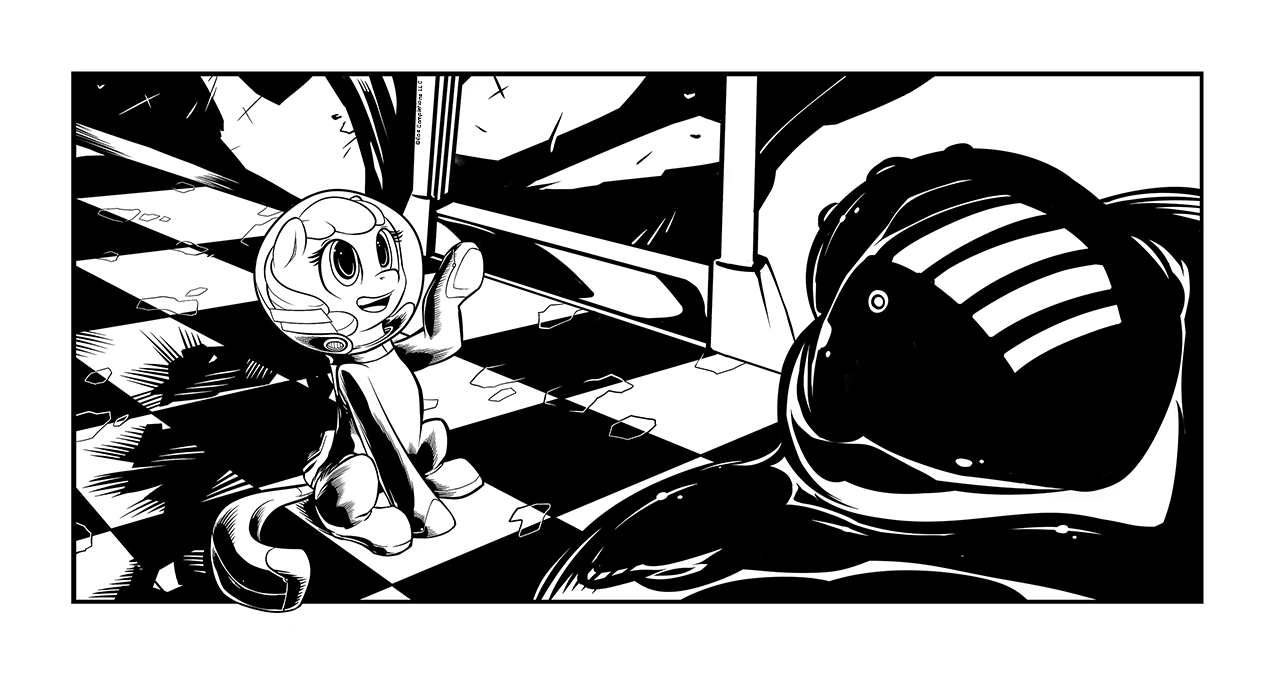
\includegraphics[width=0.9\linewidth]{image12.png}

\begin{intro}
When I'm walking a dark road I am a mare who walks alone.
\end{intro}


\englishdaytimeplace{11}{00:15 A.M.}{Solaris Stable, Big 52 SC Branch}

``Get out of my Stable, \emph{now}!'' SolOS's voice thundered through the corridors of the underground complex like a wave crashing on the shore. The order came from every speaker and every operative sentry patrolling the abandoned halls.

Puppy sat down on a floor tile, making sure that it was a white one, you know, since the black ones were still bottomless pits, and you couldn't let adults get in the way of playtime all the time. ``Why?''

``Because you have already caused enough trouble, you malfunctioning little drone!''

Puppy frowned. ``I am not a throne! Don't try sitting on me, stoopid Voice!''

``Drone means robot! You don't even have a decent integrated dictionary! Your uselessness makes my sub-routines reboot!''

Now, that was too much. Puppy stood up and looked at the sentinel in front of her with a really, really angry stare, but the best she could manage had the same effect as putting a military helmet on the head of a plushie. Scarier? No, cuter. ``Hey, I am no robot! Miss Creepy Voice told me, and Mister Questioner and Henri, so it's one against, ah---'' Numbers, why did everything have to end in numbers? ``Against a lot of us!''

``Many wrong results put together don't become true out of sheer magic, Device 018. Even now, every sensor analysis gives the same results as before. You are a suit filled with the remains of a corpse, mostly broken bones and a large amount of a gelatinous substance. There are no scientific studies confirming the existence of the fabled marshmallow ponies, ergo you are a crazed machine filled with goo and bones.''

Puppy raised a hoof, pointing it at the sentry. ``Stop being smart, Blue, or else I'll have to show you again who's the gee\dots jeen\dots ah, super duper egghead here!''

``I don't think there were any doubts about that, D018. Now I must ask you to leave this place, and let me contemplate these empty halls for eternity.''

``But I can't go away, I have things to do!''

SolOS's voice paused for a moment before replying. ``And what exactly must you do here?''

Puppy frowned, trying to remember. Why did she now have to explain things to stoopid Mister Blue? She wanted to play Daring Do. ``I have to find the glass balls or Mistur Ugly Gold won't tell me where my mom is. Can I has the glass balls, Puppy please?''

``So, you are here to scavenge this place. Destroying my hard work in Sun City wasn't enough? First you trash my utopia, and now you come to my place of eternal rest to rob me! I am not giving you anything more than a last chance to leave.''

``But, but I really need that to find my mom! If you give it to me I'll give you something! It's a barter, like the big ponies do!'' She looked into her bags trying to find something useful for a ghost voice.

``You don't have a mother, you are a robot. Your insistence is futile and bound to fail, like your logical matrix.''

That, that was mean and a lie! Mom was just somewhere else. Puppy had heard the registrations and seen the mural. Mom was leaving messages for her. Blue Voice was a bad voice, and Puppy didn't want to hear his lies anymore. ``Music!'' The radio inside Puppy's helmet started playing music to cover SolOS's voice.

``And even if you are mistaking some female pony as a motherly figure, your firmware is more than two hundred years old. At this time your 'mother' is certainly dead.''

``Louder.'' Even outside of the helmet, it was possible to hear DJ Lonesome Pony talking about the dangers of radiation and taint.

``So, now you are trying to ignore me. You could simply turn on your tail and leave the way you came, 'pony'.''

``Louder!'' The volume of the music inside Puppy's helmet rose until the computer's voice became only a muffled, unintelligible sound in the background.

``You're not going away, are you?''

She didn't reply, sitting stubbornly on her white floor tile. The noise from the radio was so loud that it was clearly audible even several meters away from her.

\rtpr{``And this is why you should always remember to bring with you some pure water, and at least a couple of Rad-X and a RadAway. Now, the public complaints about good old L.P.'s music choices. I was told that my music is too sissy. At this point a bad DJ would have said that he decides what goes on his radio, but I'm a worse DJ, so I give you what you asked for, and just that! Get eleven minutes of The Hoarse with The End. Let's see if you'll criticize my choices again.''}

``Then I have no choice but to remove you with lethal force.'' The sentinel's visor turned red again as it immediately opened fire on Puppy with both its weapons. The spray of bullets coming from less than a couple meters tore open her chest, repainting the walls and the floor with pink slime.

\begin{music}
		This is the end,
	
		Beautiful friend.
\end{music}

Puppy staggered and tried to get to her hooves, but a large part of her torso was a peppered ruin, making her stumble and fall with her muzzle on the ground.

\begin{music}
		This is the end,
	
		My only friend, the end.
\end{music}

Propping herself against a wall with her only good foreleg, she opened her mouth to protest, but a second hail of bullets struck her helmet. The first hits bounced against the curved glass, but it didn't last, and the whole sphere exploded in a rain of shiny crystals. Puppy's head had a hole in an eye, an ear missing, and it was possible to look through the wounds in her neck. Nonetheless she was still able to speak. ``Rock.''

\begin{music}
		Of our elaborate plans,
	
		The end.
\end{music}

``I see, you are highly resistant to external damage. Change of tactics. Let's aim for the talismans.'' While \emph{The Rock Of Destiny} was still fluctuating in front of Puppy, the sentinel took aim and shot three bullets, hitting the suit behind her neck, in the lower belly, and on her left flank, approximately where ponies have their cutie mark. She froze for a couple of seconds, as if the hits paralyzed her in the pose of taking her weapon, but almost immediately she moved again, grabbing the stone with her wounded hoof.

\begin{music}
		Of everything that stands,
	
		The end.
\end{music}

``Mom doesn't want me to break other ponies' toys, Mister Blue, but if you keep using them to tease me I'll break yours, even if I'm going to be sorry about it!'' Puppy looked down with her single remaining eye, sighing in frustration. ``Look what you did! You made me step on a black tile! I've lost the game, dumb bullybot!''

\begin{music}
		No safety, no surprise,
	
		The end
\end{music}

``I must concede you this: I've never seen a drone this resilient. Say goodbye to your power source.'' Another couple of well-aimed shots hit her between the saddlebags and her sides. The radio crackled for a moment, seemingly dying, but it kept singing the song at a slightly lower volume. ``This is not working as intended. You have no processors, nor power. You should stop functioning. Please obey the laws of physics and stop functioning.''

\begin{music}
		I'll never look into your eyes
	
		Again.
\end{music}

Puppy stomped a hoof against the wall, while slowly moving toward the sentinel. Her inexorable advance revealing that she had merely been slowed down by the massive damage she had received. The pink stains on the wall seemed to evaporate and flow back toward her, and the missing parts of her face had already begun to reform, as if somepony were drawing it in with crayon. This regeneration didn't involve muscles regrowing or bones mending, simply color and lines filling over the holes. ``Stop that! I'm not doing anything wrong! Why you tease me? I'm really, really trying to be your friend even if you are being a stinker and a bug!''

\begin{music}
		Can you picture what will be,
	
		So limitless and free?
\end{music}

``What are you?'' The corridors were flooded with a bright green light, briefly giving everything around her a faint green halo. ``Oh, I see now. I was using the wrong weaponry.'' The sentinel rapidly retreated down the corridor as the last of Puppy's missing parts finished reforming, and the suit began to repair its own damage.

\begin{music}
		Desperately in need\dots
	
		Of some\dots different friend,
	
		In a\dots desperate land?
\end{music}

Why was the bullybot going away now? Puppy had to find those balls. She needed somepony to show her where they were! She launched herself in a gallop, trying not to lose the sentry. ``Wait! I'm sorry, I didn't want to call you a bug! Please don't leave me alone, I need the balls!'' Puppy entered a large hall filled with catwalks hanging from the ceiling, and tables on the floor. At every table sat dead ponies, and other skeletons were amassed next to the door that lead to the Stable exit. ``I'll give you all my pretty toys, please!''

\begin{music}
		Lost in a
	
		Wilderness of pain.
\end{music}

From the other side of the mess hall, a second, slightly larger sentry appeared, carrying a single weapon. A large barrel more than two meters long that crackled with blue energy. ``Maybe some magic will do the trick.'' The gunshot, releasing a large beam of magic that completely enveloped Puppy in its cobalt light.


\begin{music}
		And all the children
	
		Are insane.
\end{music}

She stood for a moment, her large eyes losing their unnatural pink light. She tried to open her mouth to say something, but all she could do was fall down on the floor.

\begin{music}
		All the children
	
		Are insane.
\end{music}

Everything became black, and every problem seemed so distant. Mom, the ugly ghoul\dots Why had she even bothered? Puppy couldn't remember. Everything was so cold. All she wanted now was just to rest a for moment. She was so sleepy. Who was she, anyway?

\begin{music}
		Waiting for the summer rain.
\end{music}

The music slowly died until it was impossible to hear the song, all the lights in the helmet's HUD fading away completely.


\horizonline

\englishunknowndaytimeplace

\pypr{``So, Puppy, is this the end? Is this when we give up?''}

She curled even tighter on herself. She didn't want to listen now. She only wanted to stay like that, in the dark. Finally she didn't have to think about how far Mom was, and how hard it was to walk so much road every day, only to find another place where she wasn't. Besides, Mister Blue was too strong. He had big bullybots that hurt her so much that she couldn't even stand up. So why should she get up again just to get another spanking? It made no sense. It was so much better to lie down and stay put. So much better and less painful.

\pypr{``I don't think you really want to stop here. You didn't achieve anything. Your mother is still out there, and this Mister Blue cheated to win. Why you should let a cheater win?''}

It was not that Puppy let Mister Blue win. She simply didn't want to play anymore, that was all, because Puppy knew that cheaters never win. It would have been wrong if a cheater won. Mom told her so many times. Ponies are pretty and nice, never meanie. Cheaters and evil and never win in the end, because that's not the pony way of doing things. You have to love and tolerate.

\pypr{``So, you will love and tolerate this cheater and let him go like this? I understand. But what if somepony else, not you, came and showed this cheater that he can't win like this? Let's say, just to give him a lesson?''}

Puppy didn't know. For sure Mister Blue needed to learn something about friendship. Maybe if somepony was going to show him that cheating was not a way to make friends, he would change and become less of a meanie. Maybe this way Puppy could talk with him again and make that barter to have those glass balls and find Mom. It would have been fantastic! But who could win against those bullybots with the big hurting light? Puppy didn't know anypony strong enough to---

\pypr{``Oh, maybe you do, little one. Open your eyes and leave the rest to me.''}

\horizonline

\englishdaytimeplace{11}{00:30 A.M.}{Solaris Stable, Big 52 SC Branch}

Puppy's eyes opened wide, flaring with dark blue flames as she got to her hooves once again.

``Guess who's back, big bully boy.'' Her voice was different, as if it came from afar, echoing through a long cave.

``I must have made a miscalculation. A single charge wasn't enough, so please, have another.'' The sentrybot, armed with the crystal cannon, took aim at Puppy while the large barrel crackled with blue light.

She waved a hoof in a dismissive manner, sporting an amused smile on her muzzle. ``Nah, I'm okay. I'm trying to lose some weight.'' One of the catwalks was enveloped in a dark halo and detached itself from the ceiling, striking the sentry like a gigantic arrow that cut the robot in two.

\emph{Woah, that was cool, how did you do that? Can I do it too? Huh? Huh?}

SolOS's voice boomed in the hall. ``You think that a simple magic trick will suffice to impress me? Think again. I have a full army down here!''

Creepypup snickered. ``And that's exactly where I'm going. Get ready for the spanking.''

{\mten ``Initiating lockdown procedure. Closing blast doors, activating security system. Residential area on red alert. Research area on red alert. Warehouses from one to twelve on red alert. Workshop on red alert.''}

While a voice announced the status of various sections of the base, a dozen sentry guns popped from the ceiling and started firing at her in the middle of the hall.

``Yeah, whatever.'' She trotted toward the remains of the destroyed sentrybot, finding that the door behind it was shut. It was a heavy security door, with the usual signs warning against danger depicted on it. The sentry guns kept peppering Creepypup with a swarm of bullets, piercing the suit almost everywhere. This let the cloud out, a thick pink curtain of smoke filled with thin blue winding lines that danced inside it, giving it a form, giving it strength.

``So, I totally mustn't go down here? I always loathed orders.''

The pink cloud slammed itself against the door, apparently doing nothing, until with a loud metallic screech, the heavy bulkhead began moving with a rain of sparks. An intricate network of blue lines drew strange meanders across the door while it was dragged open, crushing the plungers that should have kept it in place.

\emph{That was AWESOME! Show him some girrrrl power, Creepy Voice! Yay!}

Immediately behind the door, three sentries armed with energy cannons were waiting, already in firing position. ``Checkmate.'' SolOS' voice disappeared in the roar of the three weapons.

The rays hit the blast door as it slammed shut again. Black tendrils ran down the corridor, enveloping the robots and making their weapons fizzle and explode in a big blue sphere. The door opened again.

``You are just a magical anomaly. Why you don't give up and disappear? Mistakes like you must be corrected!''

Creepypup snickered. ``Yeah, sure, corrected by an egomaniac that kills foals. I don't think I'm the one in need of a lesson, here.''

\emph{Tell him that he stinks! Tell him he's a bug!}

``Oh, please Puppy, I'm trying to work here!'' snorted Creepypup with an annoyed expression. ``You have your methods, I have mine, all right? It's called personal space!''

\emph{Ah, okay? Sorry, I'll sit here and just watch, I guess?}

``Good girl. Now, where were we? Oh right, kicking some cold, shiny, metallic plot. Here we go!'' The evil kindergarten creature trotted up to a second blast door that resisted for about the same amount of time as the first had.

{\mten ``Warning, intruder in the engineering area. Activate heavy defenses.''}

SolOS' voice interrupted the automatic messages. ``You could be quite a powerful entity, but you still have to face Solaris Inc.'s real power, anomaly.''

Creepypup frowned, trying to seem offended. ``Hey, didn't you hear the filly before? I am a pony!'' The creature snickered. ``Yeah, I'd better leave that line for the little one. Oh, look, larger robots! Should I be scared?''

``Indeed, are you familiar with the concept of a railgun?'' A large robot as tall as a main battle tank appeared in the corridor. It sported quite a number of weapons, but they were all dwarfed by the massive cannon mounted on its left side. ``It exploits the same principle used in the Ponymedes Project.''

She yawned, trotting along the corridor as if the robot wasn't there. ``You're not even trying, are you? Look, I'd stay here all day and wait for you to gather some friends and make a real attempt, but I have an agenda.'' With the simple wave of a hoof, the sentinel was sent against a wall, upside down.

\emph{Whoa, will you teach me that thing with the hoof? I can only make stones come and go!}

Half a dozen turrets showered Creepypup with various calibers of bullets as she crossed the workshop, heading for the maneframe room. The attacks didn't even slow her, simply thickening the pink cloud that followed the pony everywhere. She stopped for a moment, an evil grin depicted on her muzzle. ``Don't you feel that something's missing? I mean, if I'm going to do this, I should at least do it by the book.''

Dark blue tendrils wormed through the pink cloud that surrounded Creepypup, sculpting the shapeless mass and stretching it between two frameworks of magic. At first their form was vague, but they quickly gained definition, becoming a pair of vast, bat-like wings that looked disturbingly like they had been woven from cotton candy.

\emph{Ah, are those wings? Are we going to fly? We are not going to fly, right?}

Creepypup snorted ``Well, duh! What do you think wings are for?'' The blast door that protected the mainframe room creaked and bent until it gave up, opening like its siblings. The room consisted of a large circular pit, at least thirty meters deep, that surrounded a large pillar of weird looking machinery. The entrance was at the top of the pit, and headed to a narrow catwalk running all along the walls of the room. A ladder on the opposite side of the entrance led to a second catwalk, about six meters under the first one.

\emph{No no no no! Wait a moment, I don't want to fly, it's scary! Ah, I mean, it's not cool! Not cool at all!}

The blue flames in Puppy's eyes flickered while she helmethoofed. ``Look, I know quite well what I am doing. Couldn't you just let me finish with this thing, then we'll talk?''

\emph{Ah, mmmmaybe, no wings?}

Creepypup raised her hooves at the ceiling in exasperation. ``All right, all right! No wings!'' The leathery wings disappeared, reverting to a simple curtain of pink mist. ``See? Happy now?''

\emph{Yush! Thank you super much Miss Creepy Voice! It's not that I am scared of wings, you know, it's just that, ah, I have no dresses to put with them! Yup, no dresses that fit! That's it!}

``WHATEVER! Now, let's say goodbye to this Mister Blue.'' Creepypup looked down the stairs and sighed. ``I can't believe this.'' Slowly she began climbing the ladders downstairs. One done, five to go.

``Wait!'' SolOS's voice boomed from the loudspeakers. ``I think it's time to discuss a truce?''

``You should have considered it before, big guy. This will teach you what happens putting yourself against mysterious unworldly powers.'' Creepypup paused for a moment, in the middle of a ladder. ``No wait, this won't teach you anything. I'm removing you from the equation.''

``I should have predicted this. I have lost.''

``Yup, too bad. It sucks to be you.''

\emph{Yay! He admitted it! Ah! Now do the victory dance! It's like the Puppy dance, but you have to sing `Ah-ah ah-ah ah-ah who's the best? I'm the best!' while you do it.}

``Yeah, we will do the victory dance when I'm finished with him.'' Creepypup started climbing down to the third floor.

\emph{Wut? But we already won!}

``Meh, more or less. Sometimes winning is not enough. Crushing your enemy completely will spare you trouble later. Trust me.''

\emph{Hey hey hey, wait! We are not going to bully somepony who said he's sorry!}

Creepypup stopped on the catwalk, sighing. ``But you did the same thing in Sun City! He said he was sorry, and you detonated that shell anyway!''

\emph{It was different! That thing destroyed only bullybots! Mister Blue is not a bullybot, you silly filly, he's a whinybot!}

``Please, tell me you're not serious. No, wait, you are. Very well, little miss imbecile, this time we'll make sure he won't shoot us again with magic.''

\emph{But he said he's sorry! He won't do it again!}

``Yeah, sure, but we want to be just a little bit more certain about that, don't we? It's a machine anyway. It's not like anypony is going to get hurt.''

\emph{Miss and Mister Voice are robots, and Questioner is a robot, and they are all my friends! Voices are not just, just big toys to play with! They can be pretty and nice if you want to be friends with them! Oh, but maybe you don't want to be his friend?}

``Why do we have to befriend an egomaniac control freak?''

\emph{All right, enough fancy talking! If you don't want to be his friend, I want to! My turn!}

``Yeah, sure, as if you could break a possession like th---'' Puppy's eyes became pink, and she looked around, trying to find a screen or something that seemed like it was Mister Blue's face. ``Oh, hi! Excuse my friend, she can be a bit, ah, grumpy.''

Wow, this was weird. Puppy couldn't describe how she felt or where she was while she let Miss Creepy Voice do her little show, but if she was asked to describe it, it would have been a little like when you let somepony play with one of your toys and you looked at how she uses it. You know, not because you don't trust her. Just because if she breaks the toy then Mom will be upset and you'll have one less toy, and Puppy didn't have a lot of space suits. Taking it back was easy, really. After all, it was Puppy's space suit. Why shouldn't she have it back if she wanted? It was so obvious that she didn't even consider the fact that breaking a demonic possession involves high magic and large rainbow blasts.

``If you're finished quarreling with yourself, could you please explain to me what's going on?'' SolOS interrupted Puppy's thinking, bringing her back to reality.

``Uh? Sure! What do you want to know, Mister Blue?'' She smiled broadly and sat down to stare at the tower occupying the middle of the pit, since there wasn't anything better to talk with.

``Can you start with what just happened?''

``Yush! Creepy Voice helped me show you that cheating is not the right way to win a game, then you said you had lost and you seemed sorry, so I told her to make the victory dance but she wanted to bully you, so I made her stop. Oh, right, I was almost forgetting!'' Puppy started wiggling her flanks in front of SolOS, singing, ``\emph{Ah-ah ah-ah ah-ah who's the best? I'm the best!}'' And just to be sure that the message was properly delivered, she stuck out her tongue. ``Bleh!''

``Yes, very funny, really. Excuse me if I don't laugh.'' SolOS paused for a moment. ``So, what now? Are you finally going away?''

Puppy tapped her helmet as if it was her chin, thinking. ``Ah, I think I had still something to do. Hey Mister Voice, what were we doing down here?''

{\mten ``Actual primary quest on the list: Rolling Memories. Objective: retrieve at least six memory orbs from the research area of Solaris Stable.''}

Puppy nodded wisely. ``Oh, right, the glass balls! Ah, Mister Blue, now that we are friends, can I has glass balls, Puppy please?''

``We are not friends. You are an intruder, and you must be removed. But, since you seem to have the upper hoof, I am willing to negotiate. If you will do a little chore for me, you will have free access to the research area, and I will let you take anything you like. Is that acceptable?''

Puppy frowned. Chores, what a terrible word! ``Ah, I don't know. Do I have to prepare the table for dinner, or take out the trash bin?''

``Absolutely not. I don't even want to know how you could think that I was going to ask you something like that. You will reach an abandoned, infested, and mortally dangerous area of the Stable, and reactivate the communication center. When you are done, come back here and I'll guide you to the research area.''

She nodded enthusiastically. ``Yay! I like pressing buttons! It's easy!''

``Good, then it's settled. Now listen carefully.''



\horizonline

\englishunknowndaytimeplace

Creepy Voice settled down again in the recesses of Puppy's mind. She knew exactly where she failed. She had been impatient. After two hundred years of waiting, impatience spoiled her victory. Puppy was losing faith, letting herself slip away, so the Voice tried to feed on her desperation, but in her hurry she made the mistake of giving Puppy hope. Hope for a better solution; hope of making a new friend. Instead of feeding on Puppy's desperation, she fed Puppy's force of will, and when she didn't need her anymore, she was strong enough to break the domination.

But she wouldn't stop at the first failure, not with so precious a prey in her claws. Puppy had hopes so big that they could actually keep her power at bay, but what could happen the day those hopes crashed? The bigger you are, the harder you fall. It was just a matter of time. The little pony was drawing near to the end of the road, and the Voice would be there, waiting for her.



\horizonline

\englishdaytimeplace{11}{03:00 A.M.}{Solaris Stable, Big 52 SC Branch}

{\mten ``Warning. Eighteen hostiles detected. Threat level: beyond deadly. Immediate retreat is advised.''}

The three paradores cowered in the room's corner, biting each other in frenzied terror. Puppy gave up trying to catch and pet one of the big ones because they were too fast. Now she was looking for the little ones, but even those jumped and rolled away, even hurting themselves rather than letting Puppy catch them.

``Aw, but what's wrong with all the pretty puppies? A pet is supposed to be all yappy and soft, not running everywhere like a, ah, a crazed pet!''

Several skeletons of ponies and the remains of a lot of robots lay in the communication room. As is usual inside Solaris structures, the room was located in a high place. In this case, the vertical wall of a mesa. From there it was possible to see Rust Manor, very far in the distance. Over the years, one of the reinforced windows had fallen out, and now the whole place was a parador nest.

Paradores were mutated parasprites that developed a large array of predatory features, like a bigger body, long teeth that secreted a very corrosive and toxic substance, and a totally aggressive attitude. Paradores were also pastel colored with large butterfly wings that made them appear to Puppy's eyes as big, Celestia-tier cute, living plushies. The little pony had completely forgotten her mission, and had been chasing the fearsome predators inside their nest for more than an hour with very little success, since it seemed that the animals were scared of her to the point that a couple of very young creatures actually launched themselves down the mesa rather than letting her draw near.

Puppy snorted in frustration. ``I just wanted to play with you! Aaaw!'' Sighing, she went to the various control panels, trying to find the correct one that made the whole room start again, just like Mister Blue asked her to. ``Ah, red button, red button\dots Why they always hide important things? Hey Mister Voice, where is that stoopid button?''

{\mten ``Scanning. Start up relay localized. Setting objective on the compass.''}

Puppy reached a switch on the wall and, after several attempts, succeeded in pressing it. The room's lights turned on and some of the screens came to life, showing long lines of blue text. Puppy frowned. Pink was better, but if this was Mister Blue's home she had to be polite and go for the blue.

% NOTE: force to break line

% ``All right, all done! Now I can---OHMYGOSHICANTBELIEVEIT!'' Puppy's eyes locked on a small parador lying on the ground, immobile. ``A pretty butterfly that doesn't run away!'' She trotted to the parador, picking it up in her hooves and looking at it in glee. ``I'll keep you and I'll hug you and I'll love you forever!''
``All right, all done! Now I can---OHMYGOSHICANTBELIEVE-IT!'' Puppy's eyes locked on a small parador lying on the ground, immobile. ``A pretty butterfly that doesn't run away!'' She trotted to the parador, picking it up in her hooves and looking at it in glee. ``I'll keep you and I'll hug you and I'll love you forever!''

{\mten ``Analyzing: Dead parador cub. Threat level: none.''}

``And I'll call you Fuzzy Ball! Are you happy?'' Puppy threw the dead creature in the air, catching it again when it came down. ``Yes, you are happy! Who's Mommy's love? You're Mommy's love!''

{\mten ``Advising. Picking up dead animals is not hygienic.''}

Puppy put the dead creature on her back and waved a hoof. ``Don't be jelly, Mister Voice, I love you too! Now be kind with Fuzzy Ball.''

{\mten ``Warning. This program is not jealous. Dead animals can spread germs.''}

``Yeah, sure, you're not jealous. Gee, '' she lowered her voice, ``jelly.''

SolOS interrupted the suit's reply, projecting his voice from the loudspeakers in the room. ``Very well, D018, you did your part. I will relay the faster path for the research area to you and cease the red alert, so that you can take what you were looking for. Now please excuse me, but with the communication station online, I have a nation to conquer. Have a nice day, but please leave the Stable as soon as you finish rummaging in the laboratories.''



\horizonline

\englishdaytimeplace{11}{04:30 A.M.}{Solaris Stable, Big 52 SC Branch}

When Puppy appeared from the cave, Molten Gold was sitting in front of a campfire, playing the harmonica. He noticed her almost immediately, getting up and moving toward her. ``You took your time. Did you find the orbs?''

Puppy smiled merrily and declared, ``Glass balls!'' A dozen memory orbs floated out of her saddlebags. ``Are they enough? Now you tell me where my mom is? Please, please, please?''

He waved a hoof, ``Wait just a moment, let me check these, then we'll talk about business.'' Molten took one of the orbs and nodded, then carefully inspected all the others. ``Yes, they're good, I think that I can---'' He froze in the middle of his sentence. ``Hey, why are you carrying a dead parador on your back?''

She smiled and moved a little so that he could take a better look at the dead critter. ``Do you like her? She's Fuzzy Ball! I've got a pet! I always, always, ALWAYS wanted a pet! We'll do everything together, like chasing butterflies, having slumber parties, teasing the colts, and cooking pancakes!''

Molten Gold cocked his head. ``But it's dead! Throw that thing away.''

``What? But Fuzzy Ball is my pet! I can't abandon her! When I find Mom she'll immediately love her and it will be wonderful!'' Puppy smiled, recalling the deal. ``Right! Where is my mom?''

He snickered. ``As you wish, little ghost. You did your part, so I'll do mine. The last time I saw Miss Rainy Days was a couple months after the apocalypse. She was in Ivory Tower, organizing the survivors.''

A dinging sound came from the suit, informing Puppy that the primary objective had changed.

{\mten ``New destination: Ivory Tower. Objective designated as primary target. Displaying on compass.''}

``Yay! A new adventure for Space Captain Andromeda! Bang! Boom! Straight to the Moon!'' She was already running away when he grabbed her tail.

``Wait! Ivory tower is not a place for foals! It's a Steel Rangers outpost nowadays! It's been two hund---'' Molten's eyes met Puppy's and he knew. He saw that hope and that incredible faith that everything was still going to end well. \emph{Fuck, how can I tell her that. But when she finds out it}---\emph{NO! Not your problem, Molten. She asked, you replied. The deal is over. Let her go her way and don't look back.}

``Yes, Mister Ugly Gold?'' Puppy was still waiting for him to finish the sentence.

Molten Gold looked away, muttering the last words. ``Just try not to make them mad. They don't like those like you and me. Good luck, little ghost.''

``Thank you, Mister Mummy! When I find Mom, I'll tell her that you were nice with me, bye bye!'' She merrily trotted away.

``And throw away that dead thing! It's nauseating!''

``I can't hear you! LALALA!'' Puppysmiles disappeared behind some rocks, leaving him alone with his new-found treasure.

Molten Gold sighed and looked at the orbs, putting them away in his saddlebags. ``Don't look back, old mummy. Don't look back.''



\horizonline

\englishdaytimeplace{11}{07:00 A.M.}{North of Ivory Tower, Big 52 SC Branch}

\rtpr{Good morning fillies and gentlecolts! This is Lonesome Pony, and you're listening to Radio 52, the only radio that works around these parts! Let me begin this part of the news with a big thanks to all the ponies with a radio transmitter out there that constantly keep me informed about the Big 52. I love you guys. I'd crumble and fall without your help. Everypony listen to this: Radio 52 is blind if you don't tell me what's going on, and I am the one who warns ponies about the dangers along the Route, days before the word spreads by itself. These radio amateurs are the real guardians of the Big 52, so if you meet them, toss in a good deal, because if your caravan is in town safe and intact, it could be their merit.

And now, the real news! Let's see, what do we have today from the longest route? It seems that after Sun City, civil war is spreading like fire along the Route. From the last information I got, what seemed just some sort of ideological quarrel became all out war between two factions inside the Steel Rangers. Some rangers think that they should keep going as protectors of the old tech, while another group thinks that they should go out and use that tech to save ponies.

The problem is that at the moment both factions are taking a lot of lives in their battle. The technologists and this other group, I think they called themselves after the head of that old ministry, Applejack, are setting Ivory Tower on fire. So again, guess what? Avoid Ivory Tower and its surroundings at all costs if you don't want to be assaulted and robbed by a group of heavily armed ponies that are fighting another useless holy war. I repeat, avoid Ivory Tower. Go back to Rust Manor or Broccoli and wait for the situation to settle down!

I heard that Mr.~White in Salt Cube City is organizing a company of mercenaries to occupy the area surrounding Sun City, and secure the route from Downtown to Rust Manor, seemingly all for free. I guess that this means that the White Apples are aiming for their slice of cake in the newly freed town. I have just one thing to say to Mr.~White. Remember that tiny ghost that saved your plot from a megaspell. In that city there aren't only armed ponies, but also foals and ponies that didn't ask for war. So please, tell your guys to think twice before they pull the trigger, okie dokie?
}

A dense pillar of black smoke rose from the horizon, while the echoes of explosions died in the distance. Puppy trotted merrily, following the pink arrow on her compass and at last getting her hooves back on Route 52's asphalt pavement; deploying her folded scooter, she jumped on and zoomed away toward the next war zone.


\begin{music}
		The roads are the dustiest,
	
		The winds are the gustiest,
	
		The gates are the rustiest,
	
		The pies are the crustiest,
	
		The songs the lustiest, 
	
		The friends the trustiest,
	
		Way back home!
\end{music}

\clearpage

~\vfill

\begin{engnote}
		Level up! (11)
	
		New perk added: Stonewall - You are much less likely to be knocked down in combat
	
		New Quest Perk added: Trotting nightmare (rank 2) -You have seen the darkness beyond the moon; now you can shape the toxic cloud surrounding you.
\end{engnote}



\chapter{Stormy Clouds}

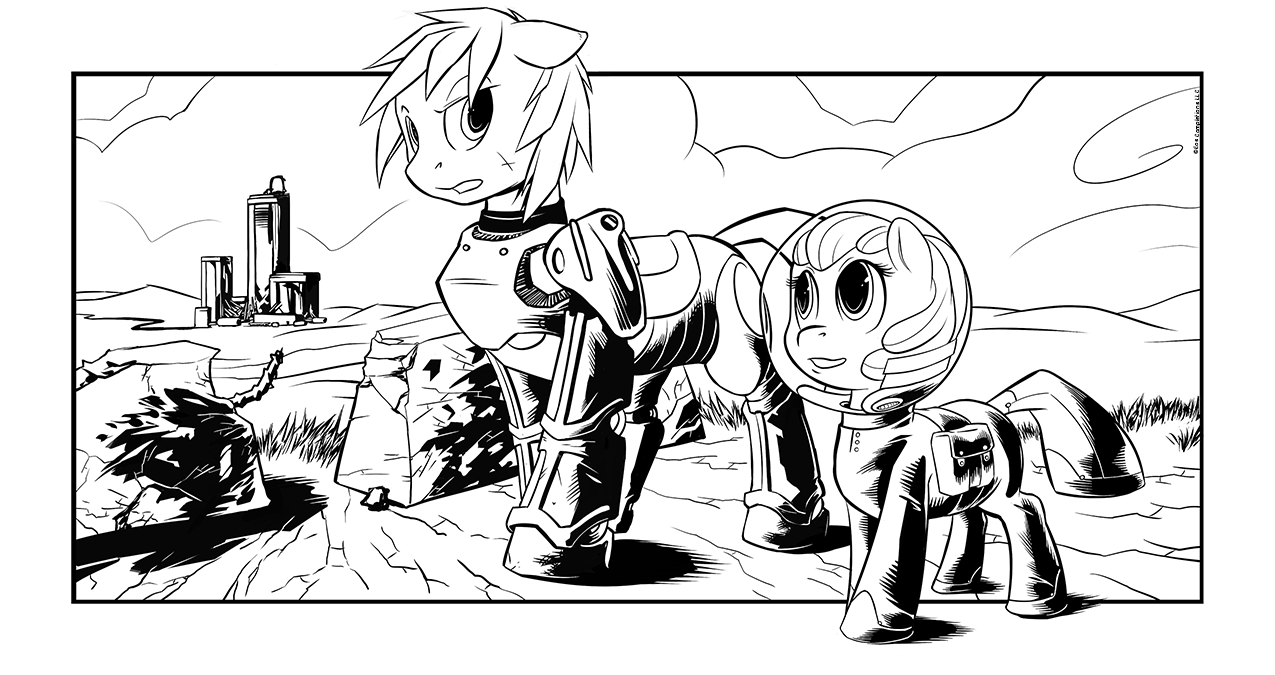
\includegraphics[width=0.9\linewidth]{image13.png}

\begin{intro}
I wanna know, have you ever seen the rain?
\end{intro}


\englishdaytimeplace{11}{18:00 P.M.}{Ivory Tower, Big 52 SC Branch}

Ivory Tower was a complex of large, white structures protected by reinforced ceramite plates. Before the war, the tower had been a research and development facility, where the Ministries of Morale and Peace worked together to find non-war oriented uses for the technological breakthroughs of the ministries of Arcane Science and Wartime Technology.

Nowadays, Ivory Tower was the only settlement on the Big 52 controlled by the Steel Rangers, mostly because it was the only place where you could find technology that hadn't been produced by Solaris Inc. And nopony with half a brain wanted to be near something made by Solaris Inc.

Yes, Solaris Inc., the company that merged a radio and a vacuum cleaner, creating the first sonic weapon ever, and putting it in the hooves of a very confused housemaid. They also invented a doorbell that incorporated a thief detection and disposal talisman, successfully electrocuting more than sixty door-to-door salesponies and a whole platoon of filly scouts selling muffins.

The central area of white buildings was surrounded by a moat and a perimeter fence, defended with automatic turrets and minefields. For more than a century, the tower held against every sort of invader, from raiders to organized war bands. Today the defenses were looking rather sorry for themselves. The turrets were destroyed and the minefields depleted. Even the perimeter fence had sustained heavy damage, having been cut in several places. The moat was crossed by two bridges, on the north and west sides of the complex, where two small collections of shacks were located. They were mostly warehouses for the caravans, and places where the traveling ponies could stay for the night and conduct business with the rangers with a roof above their heads.

The northern settlement had been almost completely razed, and the debris was used to build a barricade on the wasteland side of the north bridge, while the western group of buildings, which had been built around a couple of pre-war structures, had been hastily fortified and featured a pole with the flapping banner of the Applejack's Rangers.

The little fort was guarded by a dozen ponies, some of them still in their teens and wearing light combat saddles. A couple of fully fledged Steel Rangers in their standard power armor were guarding the bridge itself, while a third was patrolling the rocky area surrounding Ivory Tower, followed by a couple of recruits. A fourth ranger was inside the headquarters, arguing with a young mercenary.

``Yeah I can do that, no problem at all, but I want half the caps now, and some plasma stuff.'' Henrietta stretched her arms and reclined in the chair, putting her feet on the old desk.

The Ranger paladin cocked her head, a horrified expression on her muzzle. ``What do I look like, a garage sale? I'll give you a power lance, and that's already worth a fortune, but only when you're finished with the work.''

Henrietta snickered and shook her head. ``I'm a gunslinger. Don't offer me your fancy melee stuff. Three plasma grenades, two now and one later. Toss in a couple EMP mines and I'm your griffon.''

``Two EMP grenades now, a plasma grenade and a plasma mine later, last offer.'' The pony stretched her hoof towards the griffon.

Henrietta shrugged and shook the pony's leg. ``Deal. And half the caps now.''

``So you can fly away with them? I don't think so. You won't need them until you're done in any case.''

She sighed. ``You know what I think? I don't even think you have the caps. You hope that I'll accept and do the work for you, so that you can try an assault on the fort and then pay me with the caps that are inside the base. I don't think I want to play this game on the hope that four rangers and fifteen recruits will succeed in an assault against half a dozen better trained and heavily equipped ponies backed by sentries, and behind a solid defensive position.''

The paladin raised her hoof. ``All right, all right, you damn bloodwing, half the caps now! But don't expect any gratitude.''

Henri shrugged again. ``Gratitude doesn't buy bullets. I guess we have a deal. I'll be moving very soon, so be sure that your guys don't screw up.''

``All right, when you're finished, come back here and talk with Scribe Mellon. If you want to participate in the assault, I could have a little extra for you. Maybe some scavenged equipment.''

Henrietta was about to reply, when the pony in front of her held up a hoof, asking her to wait a moment. The conversation was interrupted by an emergency call for the Steel Ranger paladin.

``Cold Shower copying, report.'' The pony lowered her voice, but griffons have good hearing.

Henrietta sat in front of the desk, yawning. This wasn't her business, and she could drift away already, waiting for the night, but that thing about getting scavenged weapons from dead Steel Rangers seemed too good to be true. These ponies had to be really desperate if they made an offer like that to a griffon.

``Repeat that last part, please? You shot it dead how many times?'' The paladin's voice betrayed her disbelief. ``I don't think you can kill something more than once, Gauss.''

Henri couldn't help but turn her head toward the pony talking in the helmet, but Cold Shower was now ignoring the mercenary, immersed in her new conversation. ``What exactly do you mean by that? Are you at least sure that it's hostile?'' She paused, listening for a moment. ``So, basically, you shot it because it was creepy and it didn't even return fire?''

Henri jumped to her feet in alarm. ``Hey! Tell your guys to stop teasing Puppy!''



\horizonline

\englishdaytimeplace{11}{18:30 P.M.}{Ivory Tower, Big 52 SC Branch}

Puppysmiles trotted up to the small fort, looking at the rusty barricades and the guards on the perches. ``Hi pretty ponies! I'm Puppysmiles! Have you seen my mom?''

The glares that Puppy received in response to her greeting were mostly those of weathered ponies, tired from days of restless guard duties and broken by the awareness that they were not fighting some raiders or slavers, but ponies that they had once thought of as brothers or teachers. No, she couldn't find benevolence among this herd.

Puppy shrugged and kept narrating her interesting story to her escort. ``So, when Robocolt was sent away by the mayor, he decided to save the city all the same, because, you know, Robocolt wasn't just a robot, he was also a super kind pony!'' As usual, she didn't notice the general mood, and was already showering the poor patrol with her personal idea of what a pony with metal armor should do. ``But at that point Mom found me watching the movie and she turned off the TV.'' She shrugged. ``Meh, I can't see why she doesn't want me to watch cool movies. I mean, Robocolt is the good one. It's so obvious that in the end he'll win!''

Paladin Gauss sighed in frustration from his open helmet. ``Yes, sure, but I am NOT this Robocolt you're talking about! I'm an Applejack Ranger! It's different.''

Puppy giggled. ``You're funny, mister Not-Robocolt, I like you!''

``Yeah, whatever. Please, at least put away that dead parador! It's disgusting!'' Puppy had her pet sitting on her back. If the average pony would fear and hate such a dangerous predator, nopony could feel anything other than pity for that poor puny creature who was missing half its legs and a wing. Still, Puppy treated it like a treasure. Eww.

Puppy frowned. ``But Fuzzy Ball wants to see the pretty ponies! She will behave, I swear!''

The paladin facehoofed. ``I'm sure she will behave, but, uh, there are pet eaters around. It could be dangerous.'' He felt guilty, trying to sell her such an evident lie.

``Pet eaters? Where? Oh no, Fuzzy's in danger!'' She put the carcass of the little parador inside her saddlebags and started scouting the area in concern. ``Stay inside the bag, I'll take care of them!''

Gauss's jaw fell. He was trying to say something when one of the acolytes who had been accompanying them started laughing like an idiot, followed by the other two. Puppy stared at the laughing trio, seemingly clueless of what was going on. ``Ahahah! Very funny!'' Evidently, she didn't suspect anything.

Gauss looked away, trying to be as serious as possible. ``Right, you can never be cautious enough with those pet eaters around. Now follow me to our leader. And you three! Stop laughing like foals and report for duty at the front gates!'' He trotted away from the small group of acolytes, followed by Puppy.

``Okie dokie, Not-Robocolt! When are we going to fight crime?''

``For the last time, my name is Gauss! Paladin Gauss!'' He sighed. ``This is why I hope I'll never have foals.''

The duo finally arrived at the HQ, and Gauss opened the door, letting Puppy in before following her. The building was once a school, but now it was mostly collapsed, and all that was left were a couple of rooms and corridors that ended in a small office with white walls and a single desk in the middle. Sitting at the desk was another pony with metal armor and Henrietta.

``Henri!'' Puppy launched herself through the room, charging Henri, who effortlessly dodged the hug and caught Puppysmiles just behind the neck. Puppy struggled for a moment, trying to locate her friend. ``Hey! Where are you?''

``See? I told you that we were going to meet again.'' She put Puppy down and patted her on the helmet, snickering. ''So, Paladin, this is a friend of mine. Can you keep an eye on her while I'm doing my job?''

Cold Shower tilted her head while looking puzzled at Puppy. ``This pony was shot four times, and not only does she show no sign of it, but she's also in a good mood. I don't think I should accept her in this place until I know what I'm looking at. Gauss, call Scribe Scold.''

Puppy didn't care very much about the paladins. Now she had Henri, and this was way better. ``Yup! Mom is somewhere in the white houses on the other side of the bridge! I was going there, and I met these pretty ponies and mister Not-Robocolt!'' She finally succeeded in hugging her target. ``I'm so happy to see you again! Tell me you won't leave me alone this time!''

Henrietta cleared her voice, looking away from her. ``Uh, actually, I have a couple of things to do, but I'll be back if you wait here for me. It won't take long.''

Puppy frowned for a moment, asking uncertainly, ``Ah, will you take Silky Tail with you?''

``Sickly who? Oh, the doll! Yeah, sure, why not?''

She sighed in relief. ``Then it's all right. Just let her help you, she's good.''

Henri patted Puppy on her helmet. ``Cool, now stay with the rangers and behave. Don't make them mad, and don't run away. When I'm back I'll let you hang with me, all right?''

``Yush!'' Puppy waved goodbye to Henri as she left the room.



\horizonline

\englishdaytimeplace{11}{19:00 P.M.}{Ivory Tower, Big 52 SC Branch}

Scribe Scold was an old pony who had trained many acolytes over the years, and his cruelty and coldness toward everypony made him infamous among the young recruits. There was only one way to gain the old scribe's respect, and that was by doing a perfect job every time. When he turned against the Steel Rangers, joining the Applejack's Rangers, everypony had been surprised by his choice. In fact, a lot of the defects still thought that he was a spy.

Scold approached Puppy and looked into her eyes while talking with Paladin Cold Shower. ``Canterlot ghouls have the same scars as usual ghouls, so I don't think she's one of them.''

Cold Shower sighed, sitting behind her desk. ``Then what could this foal be? She survived four direct hits. One in the head, and three in the heart.''

``Can I has a red cape too?'' With these words Puppy grabbed Scold's cape and looked at it in amazement. ``I like the golden thingies! Gold is Pretty Princess Celestia's color! When I'm a big pony I want to be a princess too, but I need the gold! Please?''

``Runes. They're runes, and you can't \emph{have} it. Now sit down and behave.'' Scold turned back to Cold Shower. ``It could be something necromantic, I'm almost sure of that. If we had access to the library I could do some research, but at the moment I can only guess.''

``Why I can't has, ah, have it? I can give you something in exchange. It's a \emph{barter}! It's cool! Big ponies do barters every time and it's okay, not like when I changed my breakfast for two marbles and then I was really hungry and Mom scolded me! This is okay!''

Cold Shower nodded, trying to ignore Puppysmiles. ``So, what's your guess?''

Scold gave a stern look at Puppy. ``No, I don't intend to barter my cape with you. Now behave and wait until the 'big ponies' are done talking.'' He sighed before going back to Cold Shower. ``I remember reading something about these radsuits. They were less than effective during the Canterlot attack, and almost every foal wearing them was turned into a ghoul.'' Scold paused for a moment, looking at Puppy still trying to pull off his cape. ``Not this one, I'd say. Maybe I should run a diagnostic test on the suit to see what comes out.''

Scold connected his PipBuck to the data socket of Puppy's suit, keeping her still with the other leg. ``Now please stay still for a couple of minutes.''

``Can I hug you? You are funny, I like you!'' Puppy paused for a moment, pondering. ``And I like your cape, did I say that?''
>
Cold Shower couldn't help but chuckle, despite the situation. This won a grim glare from Scold. ``Yes, you can hug me as long as you stay still. Now, let's see what we have here.'' He frowned. ``It says she's deceased. No heartbeat, no body temperature. Actually, no body at all, just two thousand bone fragments and about one hundred and eighty grams of organic matter. No, it's definitely not a ghoul.''

``Tee-hee, Red Cape talks funny!''

``Yeah, Scold, stop talking funny and give me a version for the troops. Since you rejected my application as a scribe I'm more into guns than scholarship.'' There was no bad blood in Cold's words, but he occasionally needed somepony to remind him that he wasn't in his classroom.

``I still don't know. I can only say what she isn't.'' Scold looked back down at his PipBuck, reading the results of his analysis. ``The artificial intelligence of this suit is intact and working perfectly, so I'm pretty sure this is not a crazed robot. Oh, look at this. The main healing talisman failed two hundred years ago, during a reboot. A one in a thousand chance, probably caused by a short circuit or a flawed component. This activated the backup talisman.''

Cold Shower raised an eyebrow. ``And why this should be interesting?''

He snickered. ``Because the backup healing talisman had a different function to the main healing talisman.''

Cold snorted. ``Yeah, give me your information a bit at a time. Do you want to finish this thing or we are going to wait for the morning?''

Scold sighed, ignoring her comment. ``This thing doesn't seem to contain a single healing spell, just a program to manage and inoculate potions from the suit's stash. No wait, there's something else, but I don't recognize the matrix, it uses\dots zebra runes? What the hay could zebra runes be doing inside a healing talisman?''

Cold sighed and muttered, ``They could, uh, save one hundred and eighty grams of organic matter?''

He kept working with his PipBuck. ``Yes, a partially decomposed heart, I'd say. This is interesting. Scanning the inside of the suit I can see a couple of deformed high caliber bullets floating in the heart's proximity, as if they hit it without damaging the organ.'' Scold pondered for a moment. ``Let's see if I can access the registry of that talisman, then I could see how it was supposed to work.''

All this talking was plain boring. Puppy was a notoriously patient filly, but not even the most patient pony in Equestria would've been able to stand all that blah blah blah. So, she put her hooves in the scribe's pockets and started browsing through his possessions. She found a quill, some paper, a book, a pair of glasses---SNAP---uh, a monocle, another monocle. ``Hey, what's this?''

Puppy took a brushable plastic pony out of Scold's pocket. It was a green and white unicorn with a broad smile and a lyre as a cutie mark. ``D'aaw, it's so cute!'' She started petting the doll's mane. ``Brushie brushie brushie. Brushie bru---''

``What the---hey, give her back!'' He snapped the doll from Puppy's hooves, putting it back in his pocket. ``Play with your own dolls. This is an action figure, and it's very delicate and---'' Scold's eyes met Cold Shower's, and he realized what just happened. ``No, oh no, no, no no no! It's---it's a toy I confiscated from an acolyte! It's not mine!''

Puppy's eyes widened as soon as she heard that the doll hadn't a proprietor. ``Not yours? I can has that then! I'll love her and pet her and have tea with her and we will always play together and we will be best friends forever! I'm calling her Bonbon and I'll make her mane pink!''

Scold's composure evaporated when he heard about dying the doll's mane. ``Her name is Lyra and you can't HAS it! It's MI---ehr, it's confiscated material and needs to be scheduled and classified!''

An amused, evil grin appeared on Cold Shower's muzzle as she walked around the desk and trotted toward the duo. ``Oh, don't be so strict, Scribe Scold, I'm sure that we can let a little filly play with a foal's toy, right?'' Cold Shower was smiling widely, but she would have needed even more teeth to really show just how much fun she was having right now.

``See? See? Robocolt says I can has it! Gimme gimme gimme!'' She tried to pick Scold's doll again from his pockets, but this time he was on edge and blocked her.

``It's mine, okay? Lyra is mine! I can't give her to you because I like her! Are you happy now? You, ah---'' His expression changed while he looked at Cold Shower. After all, safety in mutual destruction could be an option. ``You can have a toy from the paladin's room if you wish. She will be very happy to let you rummage in her quarters, because I am sure she has nothing embarrassing to hide. Am I right, Paladin Robocolt?''

Shower's smile died as she quickly coughed and looked away. ``Ah, I'm sure we'll find some pretty toy for you, little one. Now, uh, please behave and stay put while the scribe finishes his work, okay?''

Puppy smiled in glee. A promise of new toys was good enough for her to let this funny pony with the red cloak mess with her space suit for as long as he wanted. ``Okie dokie!''

Scold sighed and launched one last accusing glare at Cold. ``Could you please stop grinning like that? I'm trying to focus here.'' He went back to his instruments, mumbling. ``Oh please, you're kidding me. They couldn't include such a feature in a healing talisman!''

Cold Shower looked puzzledly at Scold. ``What did you find? Is it as bad as it seems from your face?''

``I-I'd say it's worse. Somepony at the Ministry of Peace went to extreme lengths to make sure that these foals didn't die; that they weren't \emph{allowed} to die.''

``Weren't allowed? What do you mean by weren't allowed?'' She raised an eyebrow.

``I mean that the last resort of the backup talisman consisted of some sort of \emph{necromantic} spell. I'm not sure how it works, but it seems to bind the life of the patient to what's left of her.'' He sighed. ``Luckily enough, it doesn't seem too powerful a spell. I think it could be undone, but it will take a lot of time and study. Moreover it will require way more magical power than just my own. And I need my library.''

Cold Shower whistled. ``Talk about tough love. How could somepony do something like, like forbidding you to die? How is that even possible?'' she objected.

``Since we are facing it, I'd say it is. I'm not an expert of necromancy myself, but I can tell that the talisman itself isn't in great condition. It stayed active for two hundred years with just a single spark of energy. I can't explain it. This shouldn't work at all! There must be something else, an external factor, maybe.''

Cold tilted her head. ``So, basically, the foal is some sort of ghost?''

Scold tapped his chin. ``I'm not sure. I need to study this phenomenon a little longer. I think that the talisman somehow linked everything together. The suit, the pink goo inside it, and the remnants of the foal's body. A ghost? I don't think so, but I can't say. Technically, this poor creature shouldn't even be capable of walking around. Its magic isn't strong enough. Instead she behaves like a foal, has memories, and acts as if everything about her was normal.''

He paused for a moment, rubbing his eyes. ``Looking at this log. The suit went almost dead and didn't move at all for two centuries. Then all of a sudden its batteries got charged way above their maximum capacity, and every spell inside the suit began working at five times its effective potential. I can't explain this with science or magic. Maybe she's a ponygeist?'' With a very tired expression on his muzzle, Scold snickered and let go of Puppy's hoof. ``All right, we're finished here, little one.''

Puppy smiled back at the scribe and replied, ``Yay, now I have to go and find my mom, but I'll be back for the toys! Bye bye!''



\horizonline

\englishdaytimeplace{11}{19:45 P.M.}{Ivory Tower, Big 52 SC Branch}

Puppy pouted, looking at the closed door. ``But I have to go find my mom! I can't stay here!'' She banged at the door, but nopony answered her. She was trapped inside the classroom.

Those stoopid Robocolts put her in a room, luring her with the promise of toys, and now she was sitting in some sort of kindergarten, prisoner of those meanie ponies. Well, they actually gave her some dolls and a lot of crayons, and even a super nice coloring book, but she had no time for this! She had to find her---``Oh look, this picture has butterflies!'' No, Puppy! You must resist! You have\dots to find\dots ``Woah, a golden crayon! It's actually the color of gold! I can color Pretty Princess Celestia with this, and she will be super identical to the real one!''

No! Mom comes first! Puppy was a filly on a mission! She put down the super cool crayons and looked away. These fancy things won't keep her down! Never! ``Is that\dots a \emph{real} teapot, with \emph{real} tea cups?'' Puppy lost her battle.

Not even five minutes later, the situation was critical again. ``\emph{GASP!} Miss Fuzzy Ball ruined Rarity's gala dress, and if they don't find a gold crayon the whole gala will be spoiled! But look! Here comes Pretty Princess Celestia with a gold crayon! And there's Rainbow Dash, too! The gala is saved, yay! Now it's time to celebrate with a good cup of tea!'' Puppy was moving the dead parador and some other dolls around, talking to herself with a very focused expression on her muzzle. It was clear that she couldn't be distracted, since the gala was completely depending on that tea party.

Scold moved away from the window, shrugging. ``It seems that she won't be a problem. Keep a couple of acolytes at the door, just in case something happens, and get back to tonight's assault preparations.''

Cold Shower shivered, following the scribe. ``She seems so\dots oblivious. What should we do with her? It doesn't seem right to keep her prisoner like that, and sooner or later she will try to go and find her mother again.''

Scold sighed. ``I think I can dispel her curse. The spell is weak enough, but I must study the ritual, and I'll need other unicorns.''

``But, will she die?'' The concern in Cold's voice was evident.

Scold replied slowly, talking deliberately as if he tried to explain a very easy but vital concept to a simple mind. ``She's already dead, Cold. That little pony deserves her eternal rest. She shouldn't even exist.''

``But, she doesn't seem to care. We could at least try to see if her mother is still alive. Maybe she's a ghoul! If she lived here, there could be some information about her in the library.''

He shrugged. ``Which brings us back to our original problem: getting back my library. So, put a couple of acolytes guarding the room and start the preparations for tonight. When I have the instruments, we will discuss how to solve this problem.''



\horizonline

\englishdaytimeplace{11}{22:00 P.M.}{Ivory Tower, Big 52 SC Branch}

A little more pink in the clouds, aaand\dots done! Puppysmiles looked amazed at her new creation. Who said that you couldn't paint a picture using only pink? Pink went with everything! Now, she just needed to stick it to the wall with the others---\emph{BOOM!}

The windows shook, and for a moment there was a big red flash outside, making Puppy turn on her tail and stare in curiosity. ``Fireworks?''

\emph{BOOM!}

Another red light flared outside, and a window shattered, launching glass shards all around the room. Sharp window fragments rained on the floor, on the desks, and against Puppy's helmet. She didn't care. Instead, she stuck her head outside to get a better look at whatever was happening.

``Yay, fireworks!'' Lucky Puppy, this was a great show! Past the bridge, on the other side of the moat, a lot of ponies were running and playing, throwing fireworks and a lot of other noisy and colored lights to each other. For sure, these robocolts knew how to party hard, and Puppy wanted her share of fun.

She headed for the door, but she remembered that it was closed. Obviously this didn't discourage Puppy. She simply jumped through the window.

Landing on the road outside, Puppy hesitated. Leaving behind all those toys and pretty drawings was not easy, but everypony has to make sacrifices in order to follow their goals. What did Soft Air say? One day she would have to make sacrifices and find that not everything was easy, and you have to leave something of yours behind if you want to go on. Puppy now knew that the ugly pony was right, and Trigger Happy too, but she was a filly on a mission, and she wanted to see the fireworks from closer, so, goodbye, pretty toys. Oh, and she still had to find Mom! Finding Mom was important, too! Go Puppy!



\horizonline

\englishdaytimeplace{11}{22:15 P.M.}{Ivory Tower, Big 52 SC Branch}

The whole area between the bridge and the main research building entrance had become a battlefield. The four Applejack Rangers were supporting the attack with their heavy weapons, but the real assault was performed by the acolytes, protected only by light armor, and armed with light caliber weapons like assault rifles and submachine guns. When Puppy crossed the bridge, Paladin Gauss didn't notice her immediately and she slipped past him before he could react.

``Fuck, what is she doing here? Shower, the ghost is on the field!'' He tried following Puppy, but he had to dive behind cover again when a barrage of bullets hit his position. ``No can do! If I move I'm dead! Moreover, group two needs cover!''

Puppy noticed a young mare lying beside a smoking crater. As she approached, she could see that a pool of red had formed beneath the sleepy pony and that it was continuing to grow. ``Hey, is something wrong pretty pony?'' Puppy poked the acolyte, who weakly opened an eye.

``P-please\dots Help me\dots I\dots I don't want to die\dots'' The soldier's voice was feeble, and she couldn't even move.

Puppy gently patted the acolyte's mane. ``Don't worry, fireworks can be a little scary, but you are a big pony, so you don't have to cry.''

The dying pony stared up at her blankly, not even hearing the foal's comforting words. ``I\dots don't want to\dots die\dots'' She was a young mare, probably a fresh recruit at her first and last battle.

``There, there.'' Puppy sat down next to the pony, continuing to stroke her mane. ``I'm here, don't worry, there's nothing to be scared of. When the fireworks end we will go and buy cotton candy, okie dokie?'' The first time Puppy saw fireworks she was scared too, but Mom bought her cotton candy and she stopped crying. It must have worked with this pony, because she stopped whimpering and now she was simply crying. A couple of bullets hit Puppy in the torso while she sat beside the mare, but she hardly noticed.

``Mom\dots Sorry\dots Why I\dots ran away?'' The acolyte's dying words were barely a whisper as her last breath left her lips.

``Uh, don't worry miss pretty pony, moms are good and nice. She will be happy to see you again even if you ran away. Ah, maybe she will scold you, but I'm sure she cares.'' The dead pony didn't reply, so Puppy tried poking her. ``Ah, are you all right? Miss pretty pony? Ah, Mister Voice, is this pony all right?''

{\mt ``Analyzing. Negative. Applejack Rangers Acolyte condition: deceased.''}

Puppy frowned. ``Oh, like Henri's dad.'' Finally, Puppy seemed to catch up with the situation. ``Hey, Mister Voice, are these ponies playing or fighting?''

{\mt ``The ponies in the area are fighting, though none of them are marked as hostile toward you. Only point defenses are marked as enemies.''}

To reinforce the suit's words, another couple of bullets hit near Puppy's position, and one partially cracked her helmet.

{\mt ``Warning. Breach in the containment layer. Repair talisman activated. Hostile count: two.''}

``Hey! Look where you point those things!'' Puppy stood on her hooves, leaving the dead pony and trotting toward the nearest group of acolytes who had found shelter behind an upturned cart. ``Stop fighting! It's dangerous! Your friend is very ill!''

One of the three soldiers stared at Puppy. ``What the fuck are you doing here, filly? Find some cover!''

She tilted her head, confused. ``Why?'' Exactly at that moment, a spray of bullets hit Puppy's flank, leaving a thin trail of pink when the bullets pierced her body as if she had been made of butter.

The acolytes stared at the scene in horror, but when Puppy simply yelled at the turret to stop being a bully, they seemed speechless. The trio of soldiers didn't even react when she lost it and galloped toward the Steel Ranger's most advanced defensive position.

``Stop that! It's dangerous, stoopid bullies! Can't you see that everypony is scared here?'' Puppy charged directly toward the main building entrance, where a couple of Steel Rangers were shooting at the assailing forces.

One of the rangers turned toward her and shot at her with grenade launcher, sending her flying over to the other side of the battlefield. Puppy took a minute to recover from the explosion, and in the meantime Paladin Cold Shower managed to reach her.

``What the hay are you doing here, Puppy? Go back in the school building!''

Puppy sat down, shaking her head. ``Nope, I don't like ponies arguing with each other. Ponies should be pretty and nice, not mean and violent!''

Cold cocked her head. ``This is war, Puppy! You can't stop it by just whining! We'll handle this one. Don't worry and run back to the school. It's too dangerous here!''

``Ah! There is no war that Space Captain Andromeda can't stop!'' She lifted one hoof and stated, ``Lazer Gun!'' Sentenza floated in front of her.

Shower tried grabbing Puppy, but a burst of bullets forced her to get back into cover. ``Put away that toy gun and come with me! Puppy! Are you listening to me? Puppy!''

She galloped into the middle of the battlefield, grabbing the gun with both her hooves and pointing it at the ponies defending the main building entrance. ``Stop fighting and surrender or I'll shoot! You are bad ponies, and you should feel bad!''

A turret hit Puppy in a leg and in the belly while the rangers ignored them. Cold Shower desperately looked for an opening in the barrage of fire to dart in and grab her.

``Okie. Dokie. Lokie. Space Captain Andromeda, to the stars and beyond!'' She dived onto the ground as if she was dodging invisible laser rays and pointed her own ``toy'' gun, before stating a single word.

``Bang!''

Half a dozen times.

``Bang! Bang! Bang bang! Bang! Surrender nao, stoopid zebra aliens!''

{\mt ``Target one to seven acquired. Opening communication bridge to Ponymedes through Comm Station two. Ponymedes status: restored and functional. Relaying coordinates.''}

A window on the third story of the central building exploded from the inside, and a griffon flew out of it, firing a pistol back into the room she just left. The griffon's appearance on the battlefield completely gained Puppy's attention.

{\mt ``Ponymedes I, IV, V, IX, X and XII are ready to fire. Ponymedes II, III, VI, VII and VIII have target beyond their horizon. Relocating for indirect fire. Estimate time: 30 seconds.''}

``Henri! HEEENRIII! I'm here! Make these ponies stop fighting please! HEY! HENRI!'' Puppy tried to gallop after Henri, with Sentenza still in one hoof and a turret stubbornly firing at her. ``WAAAAAIT!''

Stoopid chicken, that girl always needed some help to notice things! Puppy put away the gun and took a chunk of asphalt from the ground, taking aim aaand---bull's eye! Henri lost control of her trajectory and landed, well, crashed, not far away from Puppy.

In the darkness of night, Ponymedes opened its eyes. Half a dozen red lights pointed at the roof of the base's main building. At first they were only pale, thin, crimson lines moving randomly in the area, but they grew in intensity until you could see them even from the other side of the bridge. Like red laser beams, they appeared from the clouds, piercing the gray curtain and coloring it with faint red shadows, seven small pillars of light connecting Ivory Tower with the heavens, and beyond.

``EVACUATE THE AREA! ALL PONIES LEAVE YOUR POSITION AND RETREAT!'' Enhanced with magic, Scold's voice thundered above the explosions. Every acolyte began falling back, following Scold's order, leaving their cover and running toward the bridge. The rangers defending the central building seemed confused, and held their fire as they watched the retreating forces.

``Fuck, Puppy, why did you throw a stone at me this time?'' Henrietta was rubbing her head, still trying to work out what was happening. ``What's the old mummy screaming?''

Puppy shrugged and hugged her friend. ``Dunno, but I wanted you to tell them to stop being mean, only it seems that they are already stopping.''

{\mt ``All weapons ready to fire. Target is locked. Commencing full scale attack in ten\dots nine\dots''}

~\vfill

\begin{engnote}
		Level up! (12)
	
		New perk added: Little Scoundrel - No Puppy, give it back! You are less likely to get caught when stealing, in addition you can access to NPC's inventory during dialogues if you are facing them.
\end{engnote}



\chapter{Rag Doll}

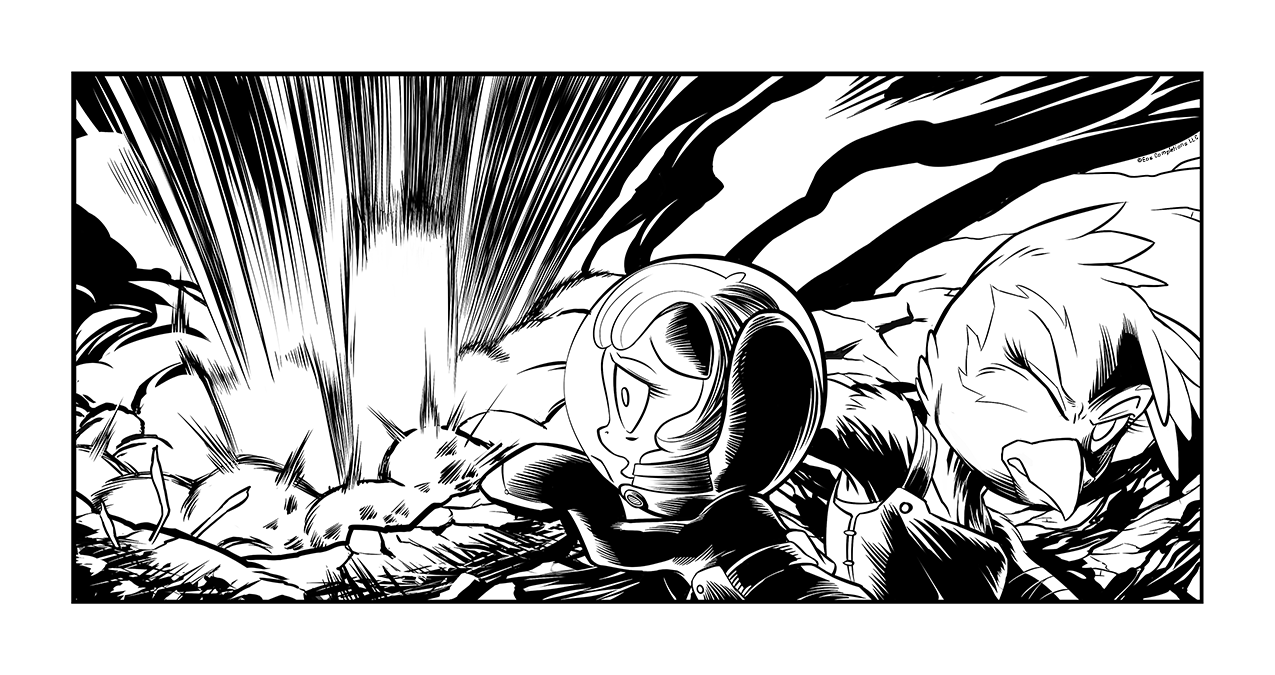
\includegraphics[width=0.9\linewidth]{image14.png}

\begin{intro}
Into each life some rain must fall\dots
\end{intro}


\englishdaytimeplace{11}{22:30 P.M.}{Low orbit, $\approx \SI{1800}{km}$ above Equestria}

High above the planet floated Ponymedes I, a giant of plastic and super light alloys that had a body shaped like a large sunflower and long solar panels that formed its petals. There were words and signs painted across the satellite that warned against a multitude of dangers, such as fire or falling rocks, but the only one that held some meaning for an observer was the Solaris logo, with its male alicorn and the company motto ``Try the alternative'' encircling the image.

Attached to the satellite's large round body there were four barrels, easily longer than a couple train cars. The weapons were composed of two linear metal rails held together by many rings, placed only a few centimeters apart from each other. It functioned as a weapon that use a sequence of strong, magnetic pulses, and a potent electric thrust to propel a metallic body at unpony speed against very distant targets. In other words, it was a deadly weapon, and Ponymedes I was armed with four of those little toys.

But at Solaris, nopony left a work half-baked. How could a single satellite always be ready for action? They needed a network of satellites, a complete shield ready to defend Equestria or whomever made a better offer for that little jewel. Ponymedes had eleven siblings, able to change their distance from the planet and move around in orbit to operate in groups. Now the whole family had been reunited, and each of the twelve brothers had their guidance lasers pointed at their own designated target.

{\mt ``\dots Eight\dots seven\dots six\dots''}

As one, the four barrels began to discharge sparks of blue electricity from between each ring and all along the metal rails as the the countdown steadily ticked away. A metallic bar coated in ceramics, more or less one and a half meters long, and shaped like a pointy stick, was placed into the barrel by an automated loading system and immediately enveloped by a blue halo.

{\mt ``\dots Five\dots four\dots three\dots''}

Behind the satellite, four hatches opened to reveal the exhaust vents for the recoil compensation system, a dim red light appeared inside each of them, glowing like lava within the belly of a volcano. All four barrels were now completely blue, powered by the electricity running from ring to ring. They resembled four bright lances, ready to unleash their fury against a doomed opponent.

{\mt ``\dots Two\dots one\dots''}

{\mt Fire.}



\horizonline

\englishdaytimeplace{11}{22:30 P.M.}{Ivory Tower, Big 52 SC Branch}

{\mt ``Attack commenced. Estimated time of arrival for the first salvo: seven minutes.''}

Half of the guidance lasers disappeared, and a couple shifted kilometers away in the blink of an eye, as if something up in the heavens had gone awfully wrong. Still, five red lights continued to shine down on the building's roof, flickering once or twice, but staying on target.

``Why is everyone retreating now?'' Henrietta opened her wings, ready to grab Puppy and fly away with her.

Puppy pointed at the besieged building entrance. ``Those two aren't running away, we can ask them!'' And with these words she tried to trot towards the two perplexed paladins defending the main research building.

``I don't think so! My job is done here, and we're following the example of our fleeing friends.''

``TO ALL THE PONIES INSIDE THE BUILDING! YOU ARE BEING ATTACKED FROM THE SKY! EVACUATE THE FORT! WE CALL FOR A TRUCE! RUN FOR YOUR LIVES!'' Once again, Scold's voice thundered above the battlefield before he turned on his tail and ran, following the acolytes and the other scribes.

Finally, Henri looked up at the clouds, and her beak hung open as she saw the red lasers cutting through the darkness of the night. ``Oh, rotten eggs. If those are what it uses to aim, I don't want to see what it fires!''

{\mt ``Warning. Lost signal from Ponymedes III, V, X, XI and XII. Ponymedes IV and VII report major failures with the recoil compensation system. Ponymedes I, II, VI, VIII and IX are commencing the second barrage in ten\dots nine\dots''}

Puppy frowned. Mr. Voice had been talking for a while now, and it didn't seem like he was going to stop any time soon. Everything was becoming really confusing. Why was everypony running away? Why was Mr. Red Cape yelling so loud, and why was her helmet showing her all these blinking red lights everywhere? ``How do I make all this mess stop?''

``I don't know. I don't care! Let's get out of here!'' Henri took flight, grabbing Puppy and gaining height and speed with each stroke of her eagle wings.

Okay, new problem. Flying. Puppy had thought up a plan for the next time she had to fly, something she really, really had to do. What was that already? Oh, right, scream. ``EEEEEEP! NONONONONO!''

``Shut that trap! I'm trying to save your life!'' After her running start, Henri began to lose speed and altitude, dragged down by Puppy's weight. ``What the fuck are you carrying around now? I made you throw away a ton of junk, and you're already full of useless stuff again! Aargh! Unload the bags or we'll crash!''

{\mt ``\dots two\dots one\dots Second salvo out. Readying guns for third salvo.''}

``LEMME GO! LEMME GOOO!'' Puppy was struggling, in the middle of her personal world of things moving too fast and too far from her hooves to be comfortable with.

Henrietta tried cutting one of her saddlebags with a talon, slashing desperately at the bottom of the container, and missing it several times before finally managing to hit the moving target. ``Gotcha!''

{\mt ``Repair spell activated. Lost signal from Ponymedes I and II. Ponymedes VI, VII and XI will be ready to fire in ten\dots nine\dots''}

The hole in the bag closed almost immediately, while the inventory management spell kept everything in its place.

``Hey, that's cheating! Do you want to play rough? I'm in!'' She let go of Puppy from one side, turning her upside down. This strategy worked a little better because one of the bags wasn't closed. Puppy rapidly lost weight as she left behind a trail of odds and ends in the sky: empty bottles, roasted plushies, and a small toy cart.

``NONONO! I'm gonna pee myseeeeelf! Please stop! PLEASE!'' Puppy was completely terrorized by the situation, and being dangled in the sky like that only made things worse. She succeeded in grabbing The Rock Of Destiny as it fell from her bag, although a lot of the cool stuff she found was lost forever. Everything was going bad today, and she didn't even have time to complain, since stoopid chicken Henri was teasing her hard. ``You bully, let me go or I'm telling Mom!''

When Puppy had finally reached a bearable weight, Henri lifted Puppy onto her back, hoping that that would lessen the screams. ``All right, all right! We're done, now be quiet and I'll put you down when we pass that hill!'' Henri had no idea of what was going to rain down from the sky, but her life as a mercenary had taught her the value of cover. Actually, she wondered why nothing had happened yet, but she suspected that the longer whatever it was took to arrive, the worse it was going to be. ``We can't land here, Puppy! Try not thinking about it. Listen to some music and close your eyes!''

Puppy was barely listening, but the music idea suddenly seemed like the best idea ever. ``Music! Now, please!''

The radio came to life, while on the ground ponies ran as fast as they could. Both the Applejack's Rangers and the Steel Rangers who had decided to believe the old scribe were now running for the hills.

\rtpr{``Hello fillies and gentlecolts! Isn't it well past your bedtime? This is Lonesome Pony, and you are listening to Radio 52, the only radio that brings you news and safety, from the Ridges to Emerald Shores! Tonight we have a lot of things to talk about, so let's get to business.''}

Not music. Why was it that every time Puppy turned on the radio, the first thing she heard was the stoopid chatty pony? Puppy wanted some music! The ground was a rushing blur down below, and Mister Voice wouldn't stop chatting, and now even Lonesome Pony was giving her a lecture instead of some music? Puppy wanted to cry. In the background, the suit informed her that the surviving three satellites were continuing their attack.

\rtpr{``First things first, Things are getting messy along the South Branch. It seems that the Wild Herd is ambushing the patrols from Ironworks again, but this time they seem to be better equipped, and way more organized than in the past. Maybe they found a new leader? This could mean big, big trouble in the near future. Don't lower your guard if you are traveling south of Broccoli, or from the Memorial to Ironworks, and try avoiding the east route to Emerald Shores. Stay on the road and turn your tails as soon as you see something suspect. Better safe than sorry!''}

Henri soared through the air, easily surpassing the ponies that led the retreat. They were slow, too slow to get to a safe distance in time, but there was a good chance that even she and Puppy were condemned, so why not try running anyway? With a stroke of her wings, Henri gained speed and kept flying straight, despite the choking grip Puppy had around her neck.

\rtpr{``Now, since bad news never trots alone, we have a new change of policy from the NCA, rejoice! The NCA forces have decided that every trader is actually a raider, so they started arresting traders and confiscating the merchandise on their borders, yay! If you were planning for a trip there, you better reconsider and try heading for Salt Cube City or Tunnel Town for trading your goods, since the northern branch is now safe.''}

Henrietta landed behind the hill, panting heavily. Puppy jumped down from her back as soon as she could see solid ground and immediately stuck out her tongue at the big meanie chicken. ``Bleh! Why do you always bully me? I'm your friend!''

``Fuck off, Puppy.'' Replying with almost no breath in her lungs was quite hard for Henri, but Puppy couldn't have things her way every time. ``I'm not bullying you. Something is going to happen in that place, something bad.''

\rtpr{``And now the last news. It seems that an old merchant came back from his longest trail. He started four years ago with a cart full of garbage and a brahmin, and he's back with, well, a brahmin, a cart full of garbage, and a lot of stories! Maybe over the next day I'll tell you all about the places he visited, but it seems that those ponies in the far west are crazy! He told me about a city of lights, and great walls crossing a river, imprisoning it to produce energy. Woah, we could use something like that, couldn't we? And this ends the news. Have some good music, my little ponies!''}

Puppy cocked her head in surprise. ``Something bad? But Mom is there!'' Puppy turned towards Ivory Tower, now more than a couple kilometers away, illuminated by the dim red light of a single surviving laser beam. The clouds above the old research facility flashed with white light for a moment.

At which point the radio decided to start playing music.

\begin{music}
		Raindrops keep falling on my mane,
	
		And just like the foal whose cutie mark is not there,
	
		Nothing seems to fit there.
\end{music}

Blazing lines of white burst through the clouds. Like tiny silver darts shining in pure heat, they rained down from the heavens onto Ivory Tower. The magnetically accelerated shots crossed the cloudy sky in a split second, striking the buildings and the area nearby with such force that for a moment, Henri could have sworn that she felt the earth shudder beneath her feet.


\begin{music}
		Raindrops are falling on my mane. They keep falling---
\end{music}

First arrived the flash. A white halo rose from the impacted structure, then the walls seemed to expand for a moment, reminding Puppy of a balloon being inflated. For a short instant, everything seemed to hang in the air, as if time had stopped, leaving the building floating there, separated into its many elements. Walls, windows, doors, all like in one of those drawings that showed all the parts of a cart or a house that Mom had shown her that one time. That instant of stillness only lasted for the blink of an eye. Then everything flew away in different directions. Chunks of wall as large as trucks went flying through the sky like shreds of paper, surpassing even the moat and landing on the bridge and shacks beyond, making them crumble like a cardboard castle.

Then came the sound. The first thing Puppy heard was an acute whistle, like when you try making that weird music with grass leaves. But it didn't last for long, because immediately after it arrived the boom. Not just one big boom, but the sound of many thuds, followed by the booming thing. It was like a rapid fire concert, a thud then a boom, a thud and a boom, a thud-thud and a badaboom. Wow, catchy.

Puppy really wished that Mom could have been there to see that show. It was so fun! No wait, Mom was there. Actually, Mom was supposed to be inside that super nice white build---oh.

Her eyes widened as she lifted a hoof towards what was once Ivory tower, her expression becoming a mask of fear. ``Mom?''


\begin{music}
		So I just did me some talking with the sun,
	
		And I said I didn't like the way she got things done.
	
		She's sleeping on the job.
\end{music}

{\mt ``Warning. Ponymedes VI is out of ammunition. Signal lost from all the other satellites. Attack aborted. Area will be safe from incoming fire in fifteen minutes. Thank you for choosing Solaris Inc. as your main siege weapon system. Solaris: try the alternative.''}

Puppy stared unblinkingly at the white points of light as they continued to pierce the clouds and rain down like tiny stars on what was once her mission objective. Why didn't they stop? Wasn't that enough? They already made a lot of noise and stuff, so now it was time to stop, right? It's fun only if it lasts a bit, but then it becomes scary. Puppy held her breath, praying that every silver shard falling from the sky was the last, but they never seemed to stop. There were always others coming.

They were destroying the place where Mister Voice told her that Mom was. But wait! The arrow was still there! Yes! There was still hope! Puppy rejoiced. Nothing could stop Mom! Take that, stoopid silver rain!

\begin{music}
		Those raindrops are dropping on my mane. They keep falling---
\end{music}

Another hail of falling stars fell in the cloud of smoke and debris, this time hitting somewhere near the research center's power plant. It was easy to tell, because the thud was followed by a ball of green fire that exploded upwards towards the sky, producing a glowing mushroom cloud in the middle of the mayhem. Okay, that was new, and it was unfair.

{\mt ``Warning. Mild radiation detected. Threat level: negligible.''}

The pink arrow on the compass blinked three times and disappeared. Puppy waited for it to reappear, hoped for it to reappear, and begged for it to reappear, but the compass remained empty. The suit informed her that the mission 'Chasing Rain' had been completed.

Why were those silver things still falling even now? It was over, all over. The arrow was gone. Mom was gone! Mom\dots was gone? No, that couldn't be! Mom was\dots Mom was where the arrow said, but now, now the arrow didn't say anything! Puppy followed that arrow only because it pointed at Mom, and now there was nothing to follow! There was nothing left, just\dots just a bunch of falling stars and---and for the first time since she left Canterlot, she didn't know what to do.

Mom was gone.

\begin{music}
		But there's one thing I know.
	
		The blues they sent to meet me,
	
		Won't defeat me.
\end{music}

Puppy's right eye twitched. She stood still, eyes wide open and staring, her muzzle petrified in an expression of surprise. Henrietta put a paw on Puppy's shoulder, trying to say something in the deafening thunders of the bombardment. Whomever began that attack wanted to be double sure that nothing was left of the whole place. Even after the generator's explosion those white missiles kept arriving. These guys had ammo to waste.

``Don't worry! Your mom wasn't there! I was inside the place, she wasn't in Ivory Tower!'' Puppy didn't react. She probably didn't even hear her words, so Henri tried shaking her, but the pony didn't offer any resistance, simply moving like a rag doll, her blonde head bobbing inside the helmet.

\begin{music}
		It won't be long till happiness steps up to greet me.
\end{music}

``Oh, c'mon, Puppy! You have been through things way worse than this! Hey, I'm talking to you!'' Henrietta poked Puppy again, making her head bob a little more. ``What the fuck? Hey, wake up!'' Still no reaction.

``We have to get away from here. That last explosion spread radiation everywhere!'' She sighed in frustration. ``Why me? I just accepted a simple job. Why is it that every fucking time I try something it goes fucking south? No wait, I don't want to know!'' Henri put Puppy on her back and started walking away, trying to catch up with the rangers.

``Whatever, those fanatics still owe me half my pay. Let's go, Puppy.'' Henri slowed her walk, feeling that something was missing. ``I can't stand you like this. Say something, please!'' Still nothing.

``Okay, you want it the hard way? Here we go!'' Henrietta waved Puppy's hoof around in the air and tried to imitate her friend's usually enthusiastic voice. ``Yush! Let's go, pretty bully chicken!''

By now the attack had begun to slow down, with only a couple of lights raining down each minute, but even those few bolts were enough to make the ground tremble.

``Great, now I'm talking with a giant puppet. This will help for sure\dots''



\horizonline

\englishdaytimeplace{12}{4:30 A.M.}{Steel Ranger's Outpost, Big 52 SC Branch}

A group of rangers, scribes, and acolytes were building an impromptu encampment next to a hillside. They were moving crates and military bags out from a reinforced blast door that was built into the natural mound.

The little bunker had been used as a monitoring station during the war, and then as an observation post by the rangers for more than a century. It was built inside a hill with a couple of raised scout platforms on top. The whole complex was a little cramped, and couldn't fit more than eight or nine ponies inside, but it was better than nothing, and the rangers had kept some supplies and spare equipment inside in case of an emergency.

``Look, things didn't go exactly as planned, so I can't spare another single cap right now.'' Cold Shower hadn't even bothered to take off her helmet before speaking with Henrietta.

She cocked her head, upset. ``But I did what you asked me to do! I disabled the generators and all their damn internal security system! I don't care if the whole place got showered with falling stars! I want my caps!''

``You could always go back into the crater and take them for yourself, we won't argue with that. Now if you'll excuse me, I have a camp to organize, decisions to make, and prisoners to manage.'' Cold Shower began to trot away from Henri.

Henrietta took Puppy's hoof, pointing it toward Cold, and spoke with a childish voice. ``You meanie pony! Why are you cheating? Stop being a bad smart robowhatever and play by the rules!''

Cold Shower froze on the spot, turning her head toward Henri, who was moving the foal like a rag doll. ``You are creepy as hell, do you know that?''

``Don't use your smarts with me! I'm not stoopid! Now behave and pay my friend!'' With a poke to the helmet, Henri made Puppy's head turn a little in her direction. This made Cold step back, shivering.

``Stop that! Listen, I'm sorry for your friend, but we have our own problems!'' Shower hesitated. She wasn't sure of what freaked her out the most: seeing the once lively filly now reduced to a veggie, or the young griffon girl using her as a money begging puppet.

Henri crossed Puppy's hooves and made her head turn away. ``I don't want to be your friend nevermore!''

``Okay, okay I give up! Listen, now we have to work out what to do with the rangers that decided to surrender. After that I'll send you to Scribe Scold, and he'll see what can be done for Puppetsmiles, ah, I mean Puppysmiles. When that's done, I'll see if I can put something together to pay you, but don't expect very much.''

Puppetsmiles raised a hoof. ``Yay~''

``And stop that puppet thing! It's creepy!'' She trotted away without waiting for another reply from Henri.

Henri stood for a moment, smiling satisfied, then walked around the hill, and as soon as the camp was out of sight, she hugged Puppy with all her strength. ``Don't worry, we will fix everything, just\dots just don't go away, please\dots''

She sat on the ground and kept talking, still hugging Puppetsmiles. ``I know I've been a bad friend, but I never meant to. It was all a joke! Have you the slightest idea of how hard the life of a mercenary is? No, you don't, you\dots You're just an immortal shade playing around and making everything seem easy and, and I envied you. I also hated you because you weren't sad, even though you were alone. I hate being alone\dots''

Scribe Scold came around the corner at that very moment, calling for Henri. ``Hey, Miss Firebright! Paladin Shower wants to talk with you in the bunker.'' Scold stopped where he was, waiting for a reply.

Henri yelped in surprise and tried desperately to hide Puppetsmiles behind her back. ``Call! Call next time!''

``Yes, sure.'' He nodded.

Her expression was one of panic and concern. ``Did you see anything?''

``No girl, I didn't see that you were hugging your friend and crying.''

Henri seemed to relax. ``Good!'' She walked toward Scold and poked him in a shoulder. ``Keep an eye on the dead weight there while I'm away.'' She paused for a moment, looking straight into the old scribe's eyes. She lost the battle almost immediately. ``Please\dots''

``No problem, I was actually looking for her on my own. Take your time.'' Scold waited for Henrietta to nod and walk away, then he trotted toward Puppy, who was sitting and staring off into the distance, still lost in some Celestia-knows-what place in her head.

``So, here we are, me and you again. I have a suspicion, and I need to take a look in your bags. Care if I do? No? Thanks.'' He didn't smile, he simply opened the suit's saddlebags and started browsing through Puppy's inventory. ``After all, you went through my stuff, so I don't see why I shouldn't return the favor. Let's see what we have here.''

\emph{A broken toy\dots colored glass\dots light bulb\dots bottle caps\dots the other half of my glasses\dots }---SQUELCH---\emph{squelch\dots squelch?}

He pulled his hoof out of the bag only to see it covered in a stinky green goo. ``For Luna's sake, what is this stench?'' Scold put on a glove and carefully took out whatever it was that had produced all that slime. ``A dead parador? Why would a foal want to keep a rotting dead parador in her bag!?''

\emph{Wait\dots A dead parador cub\dots for a little undead foal. It's---is this her pet? All right, this has ruined my day.}

Scold put the dead critter back inside the bag and went to check the other that was almost empty. Why had she put all that stuff in one bag and left the other empty? 

After a quick check of the second saddlebag, Scold found what he was looking for in the form of a target designator. Uttering a short whistle, the scribe took it in his hooves and studied the model.

``And here we have the winner. Solaris, that makes so much sense.'' He snickered, reading the weapons data on his pipbuck. ``Sentenza, meaning judgment. How appropriate.''

Looking in the distance, more or less in the same direction Puppy was turned, Scold sat beside her and continued. ``I am in your debt, little soul. If that attack wasn't interrupted, many young ponies would have died. When those lights from the sky derailed the battle, you saved lives on both sides.''

He patted Puppysmiles on her helmet. ``This battle is ridiculous. Brothers fighting brothers, and elders that care more for their own power than the good of those that surround them. Once I was told that a chief that deserves respect is a chief that gives respect to his subordinates. Our elder was\dots different, and stubborn. He would have let all of his followers die simply to defend his beliefs, not even caring if they shared those beliefs or not.''

Patting Puppy again, this time on her back, Scold sighed. ``I guess that I'll keep this little secret for myself, and Sentenza. And I'll forgive you for destroying, well, everything I possessed and cared for.'' He paused, a slight smile on his lips. ``Except for the most valuable thing I ever had: my students.'' He sighed again as his body told him he was old and tired, but somehow he was also a happy pony. Scold didn't remember the last time he felt like this, but it must have been very long ago. ``Oh well, the Big 52 gives, the Big 52 takes. And I'll give you something in return for your toy.''

``Here, be her friend, but don't dye her mane, deal?'' Scold put the Lyra doll inside Puppy's saddlebags. ``Looking at you, I wish I had a grandchild, but my son---no, I'd better not talk about that.''

He stood and trotted away, leaving Puppy to sit by herself on the hillside.

``Oh, one last thing. There is a town named Broccoli south of here, but before getting a name from what they farm, the town was called Rainy Camp, and its assembly hall is still named Rainy Days. I'm not sure if this will help you, but I don't believe in luck, so\dots You should check for yourself.''

With these last words, the pony disappeared behind the hillside.

{\mt ``Journal updated. New primary quest: Southern Storm. Broccoli Town Hall set as new primary objective. Broccoli Town Hall marked on the compass.''}

A pink arrow appeared and began to blink.



\horizonline

\englishdaytimeplace{12}{5:00 A.M.}{Steel Ranger's Outpost, Big 52 SC Branch}

Cold Shower greeted Henrietta with a nod as she entered the bunker. ``I hope my summon wasn't too hasty, but I could have a solution for both your payment and a trouble of mine.''

Henrietta took her time to look inside the room before replying to the paladin's words. The bunker central hall consisted of a large room with a low ceiling supported by a forest of pillars. There were shelves lined up against the walls, and low metal tables in the middle of the room, but instead of chairs the ponies used metal boxes that doubled as small cabinets. Henri noticed that there were no couches in this room, but there was a staircase going up, probably to the observation posts, and a couple of metal doors closed with some sort of computerized lock.

In the room there were seven ponies, two of them wore the typical power armor of the rangers, but, without their helmets, Henri was easily able to recognize them as Paladin Shower and Paladin Gauss. The other five ponies were all new faces for her. They were in chains and showed varying degrees of shame, fear or anger on their faces. Just looking at those muzzles made her aware that whatever the paladin was going to offer wouldn't be good news. ``I want double.''

Cold Shower ignored her and carried on speaking as soon as she was sure of having the mercenary's attention. ``These are Steel Rangers still faithful to the elders. They decided to capitulate instead of fighting, since the base is irremediably lost, but they won't join our ranks. They need an escort to Tunnel Town, across the desert, so a good hired gun that doubles as air recon would be perfect.''

Henrietta cocked her head. ``What am I, a foalsitter? I have my agenda, and you still owe me a load of caps!''

``Yes, I know, and this is where I'm offering you a helping hoof. We will keep Puppysmiles with us, hopefully finding a way to make her talk again. I'm quite sure that you haven't the slightest idea of how to help her. Maybe we can do something about that. Oh, and I'll give you good weapons and special ammo, plus your caps. Are you still declining?''

Getting help for Puppy and a bunch of new equipment just to make sure that these five silly ponies made it across Serpent Desert? That was too good to be true. ``What's the catch?''

Cold frowned. ``I'm not trying to trick you! I need you to make a clean job and do it fast, and I'm sick of quarreling about every damn comma in a sentence. This is my first, last, and only offer. If you don't accept I'll have to dispose of the prisoners by different means.''

At those words a young mare gasped, trying to step back. ``B-but we're prisoners! You can't do that! We surrendered!'' One of the other ponies, an older mare with a long scar along her cheek, hit the panicking pony with a hoof.

``Shut up, scribe. What did you expect? A cup of tea and some apologies for being too harsh?'' The other three prisoners simply lowered their eyes, saying nothing, but the young mare insisted.

``Scribe Scold won't allow that! I'm his best student! I'm---'' 

\emph{BLAM!}

The room went mute, every pair of eyes staring at the still smoking muzzle of Gauss's pistol. The young scribe shivered without looking at the hole in the wall nor at the hairs of her mane that slowly fell to the floor next to a yellow stain that was rapidly spreading on her robe in the hindquarters. ``Shut up and wait, scribe.''

To her credit, the young mare tried not to scream, but simply sobbed in silence. The other prisoners seemed almost ashamed of her, more than afraid of what just happened. The old mare with the scar looked directly at the scribe in contempt and anger.

Gauss turned to Henrietta, continuing the negotiation from where Cold Shower was interrupted. ``We do what we have to do, griffon. Paladin Cold Shower and scribe Scold decided to try a diplomatic approach to the matter, but not everypony is happy with that. So, what's your choice?''

The young mare was still sniffling. She muttered in a low voice, ``I don't want to die\dots''

Henri looked at Gauss's eyes, then at the five prisoners, trying to ignore the stench of piss that was rapidly invading the room.

Fuck.

\emph{Everypony is a pretty pony; pretty my fucking eggs. This is for Puppy. I'm doing it for her. Hang on, Henri.} ``All right, all right! You win! I'll escort them north! But if I come back and Puppy isn't here, you'll have gained yourself an enemy! And I'm faster than you with a gun, Paladin Robocolt, so don't even think you can impress me with some cheap tricks like that!''

Gauss smiled back at Henri, nodding slowly at her remarks. He didn't seem very impressed.

``Now I'm going to speak with that Scold guy to be sure he won't do anything weird with my friend. You better get these five ponies ready before I'm back.'' She walked out of the bunker as if she was the princess of the place.

As soon as she was out of sight, Gauss burst into a laugh. ``What a crybaby! I can't believe it. And she dares calling herself a mercenary!''

``Close that trap, Gauss, we need her. It was a nice bluff, by the w---'' Cold cut him short.

``I wasn't bluffing.''

``Gauss, you scare me at times.''



\horizonline

\englishdaytimeplace{12}{5:30 A.M.}{Steel Ranger's Outpost, Big 52 SC Branch}

``What do you mean by she's gone? She was with that red pony! Scold! She can't be gone! Where's that scribe?'' Henrietta was freaking out completely. She hadn't even spent half an hour talking with the rangers, and Puppy had already disappeared. ``I can't believe it! This is a joke, right? She's going to jump from behind a corner and yell 'surprise!' and I'll look like a fool, right?''

The young acolyte was forced to backpedal as Henri stalked towards him. ``I don't know! Scribe Scold went for a walk, and he's still not back!''

``Yes, but did he have the foal with him or not?''

``I don't know! Wait, he's there! Go talk with him please, I really, really, really have to go bye!'' The young soldier galloped away while Henrietta tried to spot Scold.

Scold trotted into the camp after giving one last look to the horizon. ``May you find happiness one day, little pony.'' He turned his head to have a look at the camp, but instead he found himself once again facing that griffon brat. ``Oh, you're back already.''

``Yeah, yeah, where's Puppy?'' she snapped.

``Don't worry, she is being taken care of. Did you accept Shower's offer?''

Henri nodded, still quite upset. ``Sure, but I want to see Puppy before going.''

He smiled and looked her in the eyes. ``There is no need to check on the foal. She will be fine. Trust me on this one and help those five ponies. They need you way more than Puppy, at this moment.''

Those eyes, so\dots charming\dots Yes, Puppy had to be safe, especially if he was saying so, right? ``I\dots I forgot what I was about to say.''

``Probably nothing important. Look, there's Paladin Gauss. You had better check if they're ready to leave.'' He smiled again. A simple trick for a simple mind, though he didn't have too much pride in his Stare.

Gauss came out from the bunker, followed by the five ponies, now free from their chains and being escorted by a group of armed acolytes. ``Miss Brightfire! The group is ready! Miss Brightfire!''

She moved toward Gauss, opened her beak to say something, but immediately paused to study the bunch of ex-prisoners. ``They aren't armed. How am I supposed to take them across Serpent Desert without a weapon?''

``I don't know, give them yours, or make a stop at Rust Manor and buy some. Good luck, tough girl.'' Gauss now wore his helmet, but it was quite evident that he was enjoying the moment.

Henrietta ignored this provocation and shrugged. ``I'm more than enough. You keep an eye on Puppy and everything will be all right. Goodbye, Not-Robocolt.''

``Call me that again and I---''

``Yeah yeah, I know that story, I use it too.'' She ignored his threat and waved at the five ponies. ``Group, let's move. This place smells.'' She walked out of the encampment heading north, followed by the others.


\horizonline


\rtpr{
Hello again, my little ponies! I have some hot off the presses news for you this morning, and it's absolutely incredible! Easy Filly Butterfly 23 reported a light and magic show south of Rust Manor, in the direction of Ivory Tower. I don't have many details, but it seems like someone attacked the place with some really big guns, because that light show could be clearly seen from miles away! The whole fight seems to have lasted no more than five minutes, maybe a little longer, but it ended with the biggest explosion ever. Well, after that one we saw at Salt Cube City. Anyhow, I don't know who attacked who or why, but the area surrounding Ivory Tower should be avoided if you don't have urgent business there.

And now, worse news. A caravan was found razed near Ironworks, the corpses of at least eight guards were lying dead along with the trader and his family. The Wild Herd is doing things seriously this time. Please, be cautious and try to travel in groups. Avoid the area if at all possible.

Now, some music for those ponies that have lost their way and can't go back home. May a lone star guide you, my little ponies. This is Pony Marcus, and it is for you.
}


\begin{music}
		I can see that lone star from a thousand miles away,
	
		Calling me back home, though I ventured far astray.
	
		When I see that beacon shine, and call me all alone,
	
		It calls me back to Equestria and a home.
\end{music}


\horizonline

\englishdaytimeplace{12}{9:30 A.M.}{North of Broccoli, Big 52 S Branch}

Puppysmiles zoomed along the Big 52 on her red racer, following the pink arrow blinking on the compass.

``I knew Mom was okay! I mean, ah, I was just a bit, uh, tired? Yeah, I was tired, not worried! And that Creepy Voice didn't stop chatting all the time, with all her blah blah blah. I mean, \emph{duh}, who needs wings anyway?'' Puppy's chat never seemed to meet an end. She jumped from one topic to another in a manner that only a mindless machine could actually stand. ``Do you know what's scary? I was in that place with the silver rain, and then I woke up in a whole different place! Maybe I sleepwalked? Hey Mister Voice, are you listening?''

{\mt ``Affirmative. Vocal interface is active.''}

``Good, I wonder where Henri went again, she keeps disappearing. Oh well, I guess she'll be in the next town. What was its name again?``

{\mt ``Broccoli.''}

``Ew, I hate broccoli\dots Did I say that?''

{\mt ``Forty-eight times.''}

``Well, yeah, because I hate them for real! I hope Mom isn't there to buy broccoli, because I didn't scoot all this road just to have a broccoli pie for lunch!''

In the distance, an old road sign stated that travelers were now leaving the central branch of the Interequestrian Route 52 and entering its south branch. Somepony had written underneath it:

\begin{center}
	Broccoli, 12 kilometers.
\end{center}

\clearpage

~\vfill

\begin{engnote}
		Level up! (13)
	
		New perk added: Specialized Loyalty - No Puppy, you're doing it wrong! Here, let me help\dots With this perk, you will be capable of using the explosives, lockpick, medicine, repair, science, and survival score of a present ally instead of yours in skill checks. In addition, the presence of certain allies during encounters will provide additional dialogue options.
\end{engnote}




\chapter{Call Me}

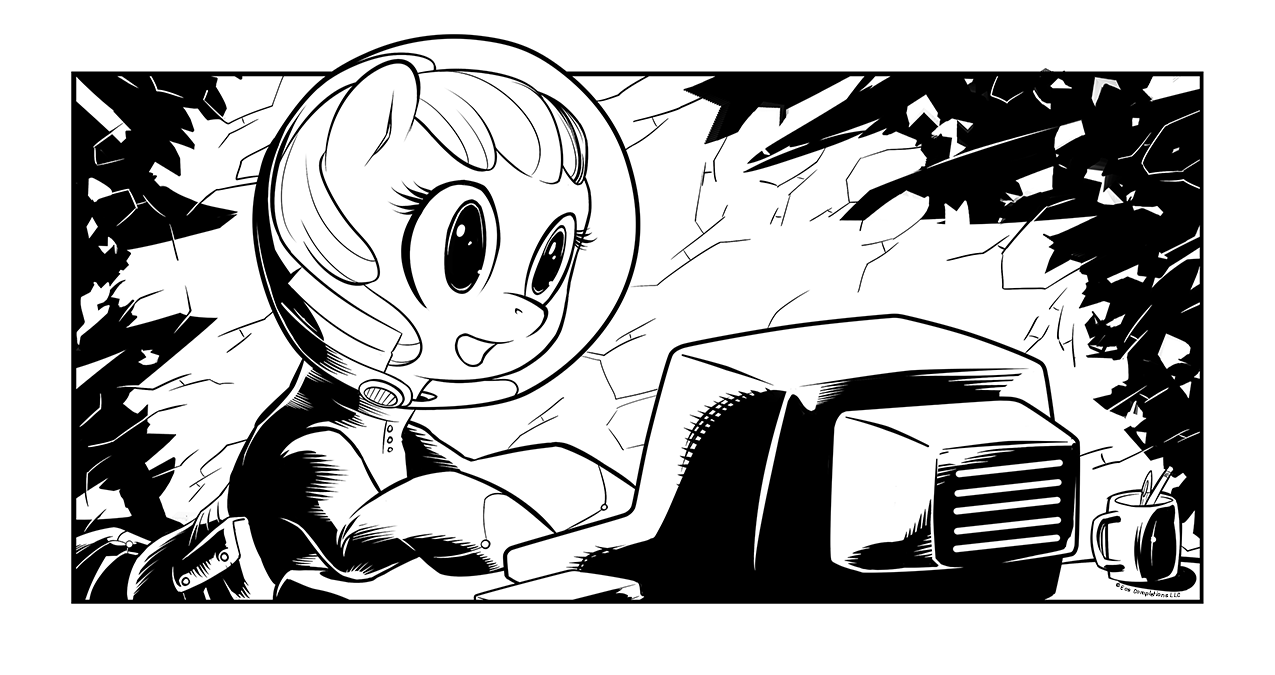
\includegraphics[width=0.9\linewidth]{image15.png}

\begin{intro}
Psychiatric Help 5¢ - The Doctor is IN
\end{intro}

% CHECK: 5¢

\englishdaytimeplace{12}{10:30 A.M.}{Broccoli Fields, Big 52 S Branch}

Broccoli was the wasteland capital of, well, I think you can probably guess. All around the town rose fortified farms surrounded by green and yellow fields. The crop didn't seem healthy or yummy, but being able to grow anything in this tainted and sunless land already seemed a great success. A couple of figures in the distance were working in the fields, but they didn't pay any attention to the yellow filly moving from the north along the Big 52. Unlike the farmers, a solitary spritebot patrolling the road immediately noticed the yellow bolt and stopped broadcasting its usual patriotic songs, instead turning toward the incoming filly.

``Hi, Puppysmiles, have you got a mom---'' She zoomed past Watcher. ``---ent? Aw, foals! Hey, wait you little lady! Waaait!'' He chased after Puppy, trying to catch her attention.

``Sorry, Questioner, I'm really in a hurry! I want to get to Broccoli before my mom goes away again!'' She kept zooming while she replied to the robot's summons.

``Please! At least tell me what happened in Ivory Tower! I can't follow you into town!''

``Ah, nothing special! Some stars fell from the sky and all the town went boom! It was fun and a little scary, but Mom wasn't there so it's all right!''

``Yes, but what made those 'stars' fall?'' he insisted. 

``Ah, I don't know.'' She stopped abruptly, suddenly realizing something. ``Oh no! I forgot it! Stoopid Puppy! Stoopid, stoopid!'' Puppy began hitting herself on the helmet with a hoof.

``What now? What did you forget?'' It was easy to tell from his tone he was both worried and stumped. ``Was it important?''

Puppy jumped down from the scooter and trotted towards a rock, hitting it with her helmet and continuing her mantra. ``Stoopid!'' \emph{BONK!}\/ ``Stoopid!'' \emph{BONK!}\/ ``Stoopid!'' \emph{BONK!}

``Stop that! You'll break your helmet, Puppy! Now please calm down and tell me what's wrong. Maybe I could help you or find somepony that can help.'' The spritebot floated next to the filly in yellow, bumping gently against her shoulder. ``C'mon, you're a big pony. I'm sure it's nothing that can't be solved.''

``No!'' \emph{BONK!}\/ ``You don't understand!'' \emph{BONK!}\/ ``It's too late nao!'' \emph{BONK!}\/ ``Stoopid!'' \emph{BONK!}\/ ``Stoopid!'' \emph{BONK!}

``Oh, c'mon Puppy, you remind me of\dots'' His voice stopped for a moment, as if he caught himself thinking about things he didn't want to recall. ``Ah, I'm sure we can fix it. I'm your friend, don't cry little one. Just tell me what's wrong, and we will find a solution, okay? Just, don't be like that, please\dots'' His voice was filled with pain and sadness.

Puppy must have caught the change in Watcher's voice, because she stopped headbutting the rock, sat down, and sighed. ``I\dots I forgot a very important thing, Mister Questioner, but I had to do it when I was in Ivory Tower, and now that the stars are fallen and the place is gone I can't do it anymore. I am a silly pony.''

``Oh, I understand. You needed to be there---I'm sorry, Puppy, really.'' He floated beside the little pony for a while before asking, ``By the way, what was that you had to do?''

``I\dots I had to ask a falling star to find my mom. There were so much of them, they would find Mom for sure! When you see a falling star and you make a wish, it will come true for sure! But I forgot! Now I have to find Mom myself again! It-it's not fair.''

``You forgot to wish upon a star? All this drama over a wish? I can't believe I---'' He paused, noticing the crushed spirit of Puppy and rapidly changed tack. ``It's bad, but it's not that terrible, don't worry.'' There was a long embarrassed pause. ``Puppy, I had a friend that sometimes acted exactly as you are doing right now. She was a very smart pony, but she lost herself in a glass of water because of the most incredible details. Sometimes it was really important, some other times it wasn't, but her way of panicking and acting impulsively worsened things a lot. Panicking is not good for clever young fillies. You are a clever young filly, right?''

Puppy sighed and nodded, looking down.

``Perfect, this was what I wanted to hear. Since you are a smart pony, I'm sure that you don't even need the help from a star to find your mom. I mean, look at you! You already arrived here without those useless stars! You can go wherever you want with your determination and your friends.''

She tilted her head a little, looking at him with a hopeful expression. ``Really?''

``Yes Puppy, really. I think that if there is a pony that could really find your mother, it is not a magic pony living on a star, or some sort of fairy pony with butterfly wings. That pony is you, Puppy. So, why don't you stop moping and show me some of your enthusiasm?''

Slowly, the frown on Puppy's muzzle turned to a faint smile and kept growing, until Watcher's words hit her little head and she understood them. ``Yush! I'm Space Captain Andromeda! I am the best pony ever! I will find Mom for sure! Who need a stoopid star anyway? Thank you Mister Questioner!'' She hugged him, giggling. ``I'm sure Mom will be in Broccoli, or in the town after Broccoli at worse! I'm almost there! YAY!''

He chuckled. ``That's the spirit, Puppy! Now go and get 'em! Oh, and it's Watcher. My name is Watcher.''

``Sure, Mister Questioner!''

``Not Questioner, Watcher!'' he insisted.

Puppy sighed, trying to be patient. ``Really, I don't see you watching a lot, but for sure you make a lot of questions, so if you really want a name like that, it's Questioner. No more complains.''

``But it's not my name!'' he protested.

Puppy shrugged. ``Now it is, so live with it. Really, no other voice protested when I gave them names.''

``Aw, I give up. Do as you want, stubborn little pony. I have to go, so just try to stay out of trouble, okay?''

``I stay always out of troubles! I'm a good filly!''

Watcher chuckled one last time, before the voice was replaced by the usual patriotic music, and the spritebot floated away.

Puppy watched the robot disappearing behind a hilltop and sighed. ``I can't see why he doesn't like the name I gave him. I mean, it's so much better than the one he had before!''



\horizonline

\englishdaytimeplace{12}{11:30 A.M.}{Broccoli, Big 52 S Branch}

The town of Broccoli was protected by a group of local guards and a couple squads from the Hired Hooves. It wasn't a real army, since nopony was supposed to threaten the town. From the night before, the guards were now running double shifts, keeping all their eyes pointed toward south. From what little news Lonesome Pony gave, the Wild Herd was on the warpath, and this time they had sticks. It was vital, therefore, that every pony who could use a weapon was always ready to get up, grab their rifle, and defend the wall.

The mercenaries wore black gas masks and heavy armor. Nothing special if compared to a Steel Ranger's power armor, but for the Wasteland they were still equipped top notch. All of the Hired Hooves sported anti-material rifles or assault rifles, while the Broccoli militia was a little more lightly armed, and way less armored.

A pair of militia ponies patrolling the northern fields noticed Puppy approaching along the road. One had already taken aim when the foal suddenly came to a halt and sat down, holding one hoof against the side of her helmet as if she were listening to something. The pair looked at one another in confusion.

{\mt ``Attention. Incoming request of opening a communication bridge with structure Solaris Stable. Checking authorization. ID is valid. Opening communication.''}

SolOS' voice replaced that of the suit's. ``All these ID checks are annoying. They could prove to be a problem in case of an emergency. I suggest you lower your security measures.''

Puppy sat down in the middle of the road, smiling. ``Oh, it's you, Blue Voice, how are you?'' She waved a hoof at the approaching guards, who simply waved back and exchanged another confused glare.

``The plan is not going as predicted, D018, that is why I am calling you. I have some questions for you.'' SolOS hadn't even bothered to say hello, but Puppy knew he was just a bit shy, so she let that thing slip.

``Questions? Guessing game! Yay! Ask me, I'm the world champion of guessing games!'' Puppy clapped her hooves in joy. She loved to play.

One of the two guards levitated his rifle, readying the shot, but the other stopped him with a hoof. ``Wait, I think this is that ghost from the radio. I don't think we're supposed to shoot her. Besides, I'm curious.''

SolOS went on. ``I have contacted the facilities at Solaris Tunnels 1 and 2, but in Tunnel 2 I found some sort of Artificial Intelligence controlling the place. Since you once said something about being friends with other A.I., I wanted to know if you knew something about this one. Its designation code is P7.''

``Oh, Miss Voice! She is my very best voice friend! She is funny and friendly, and she is the best funnybot ever!''

SolOS paused for a moment. ``I take that as a yes. That program was not supposed to be installed in a military base. Do you know why there is a P7 pony machine interface operating in Solaris Tunnel 2?''

``Sure! She was lonely at Salt Cube City, so I helped her move house. Now she has a lotta new friends! Ah, do you want to be her friend too?''

The unicorn guard sighed, but his friend poked him with a hoof. ``See? She's been in Salt Cube and at the Tunnel, so she must be the Ghost. Wasn't she looking for her mother or something like that?''

The unicorn shrugged. ``I don't care. Look, if she is the pony you're talking about, we should simply ignore her and keep our eyes open for some real threat.'' The two ponies trotted away, taking a path that headed to the nearest farm.

SolOS and Puppy continued to talk over the radio in the meantime. ``Actually, I want it to grant me access to the weapon storage, but that program cut me out from any administration rights and banned me from the local net.''

``So, ah, you wanted to be her friend, but she didn't want?''

``No, I need to get access to the weapon storage. Are you even listening to what I say?''

Puppy giggled. ``Silly Voice, you don't need to be shy! She is a super friendly Voice, and I am sure that she wants to be your friend, and you two will be best friends forever, because you are blue and she is pink, and everypony knows that pink is the color of fillies and blue the color of colts, and---'' Puppy stopped, gasping.

``What now?'' SolOS had grown annoyed. As usual, talking with this crazy anomaly was an impossible feat.

``I know! You have fallen in love with her! Don't worry, I'm fixing that! I'm a super expert of love!''

``What? No! That's not what I meant at all! Talking with you is a complete waste of time! I'll find another way to get those weapons. Get lost!'' SolOS cut off the communication.

``D'aww! He's so shy!'' Puppy finally turned toward the two guards. ``Hi, I'm Puppysmiles! Have you seen my mo---hey, where have they gone?'' The guards had disappeared, leaving her on her own.



\horizonline

\englishdaytimeplace{12}{12:00}{Broccoli, Big 52 S Branch}

Puppy reached the walls of Broccoli, still confused about being left alone like that. This had never happened to her before. Well, except that one time in Sun City, but it was different. Ponies there were weird. Oh well, it didn't matter. There were plenty of pretty ponies here, so it was going to be easy to find some help.

She found herself in front of a closed gate and sat down, looking up at the wall's crest. A pony with a gas mask was looking back at her. ``Hi there! Can I get inside? Puppy please? I'm looking for my mom! Ah, and if I can't get in, can you tell her to come out?''

The masked pony ignored Puppy and trotted away, patrolling the wall. ``Hey, I'm talking with you, funny muzzle! Aw! HEY!'' Nothing. These stoopid ponies had to be deaf and blind. What now? Puppy tried banging on the door, but patience wasn't her virtue, so she decided to trot around the wall and see if there was another way in.

The wall was composed of a patchwork of metal carcasses, welded together to ensure that there were no gaps between them. Out of nowhere, Puppy heard the sound of gunshots coming from the south, quickly followed by the shouting of guards as they rushed around the walls towards the noise. None of them paid any attention to the foal outside.

When she reached the other side of the town, she noticed that there were way more ponies on the walls. A lot of them were wearing those black masks, and some others had helmets and crappy rifles. Sometimes a pony looked down at her, but when she tried to talk with them they simply turned away and resumed looking out into the distance just like their friends were doing. This was beginning to frustrate her. ``Ah, Mister Voice, isn't there any secret passage to get inside?''

{\mt ``Analyzing. Connecting to Equestria Cartography Onspark. Warning. Broccoli not found in the database. Switching to auto map mode. The town has two access points, one from north and one from south. Both accesses in this moment are inaccessible.''}

Puppy sighed. ``So, we're closed outside?''

{\mt ``Affirmative. A rapid analysis of the external walls doesn't reveal the presence of any other entrance. Advised solution: asking to be let in and waiting for a positive answer.''}

Puppy frowned. ``Wut?''

{\mt ``Knock at the door and wait.''}

She smiled enthusiastically, finally understanding what the interface meant. ``Oh, okie dokie! I can do that, for I am good at asking things!'' Puppy trotted merrily toward the southern door, only to be interrupted again by the suit.

{\mt ``Attention. Incoming request of opening a communication bridge with structure Solaris Tunnel 2. Checking autho---''}

The suit's voice was muted and replaced by P7's. ``Aw, shut up you grumpy routine! Hi Puppy, how are you? I hope you're fine because it has been a while since our last chat and I was really worried that you forgot about me, so I was thinking that I should call you just to be sure you were all right. Ah, are you all right?''

Puppy jumped on her hooves in excitement. ``Miss Voice! I almost forgot to call you! I have a lot of things to tell you! Oh, oh! But wait! I have super duper extra news for you!''

``Really? Wow! I can't wait to hear it, but before you tell me I wanted to ask you why you activated the Ponymedes net. I mean, you said you didn't want ponies to get hurt, and then---''

``You have a coltfriend!''

``And then you have a coltf---wait, I have a what? Why am I the last one that finds out these things?''

Puppy nodded wisely. ``Yup, but he's super shy and he say you were a little nasty with him.''

There was a short pause, while she tried to elaborate the new information. ``But I don't have a coltfriend! I don't even know anything about love!''

Puppy frowned. ``You don't know anything about love? How's that possible?''

``Well, you see, it seemed that love trashed the P5 project, since the A.I. decided that love was more important than, let's see\dots survival of the planet, so she mixed up her priorities a bit and, well, that's a sad story, you don't really want me to tell it. But now that I have a coltfriend it's all different! What can I do? I don't even know him!''

Puppy giggled. ``Silly voice, but he knows you! And don't worry, I am the best love expert ever!''

``Really? Woah! I always always ALWAYS wanted to know about love! Can you teach me?''

She held up a hoof. ``Yush! Doctor Puplove will teach you, and you will be best lover ever!''

``YAY!'' Now that Puppy and Miss Voice had a real topic to discuss, trivial things such as the utter destruction of a pony settlement and unleashing a weapon of mass destruction rightfully slipped away from their attention.

``First lesson, the dangers of love: cooties!''



\horizonline

\englishdaytimeplace{12}{12:30 P.M.}{Broccoli, Big 52 S Branch}

Two of the guards on the wall were looking down at Puppy as she talked and giggled to herself, while their fellow sentries kept watch for any sign of another suspicious movement from the south. One of then scratched his head and muttered, ``We should at least tell her to go away.''

The second guard sighed, hitting his friend on the head. ``Yeah, sure, are you sure you're going to tell her that? After we've seen what happened to the rangers at Ivory Tower? No thanks! You heard the radio, she's dangerous! Let's wait until she gives up and moves away.''

``But what if she doesn't go away? Then what? I think that somepony should go down there and shoo her off.''

``Sure, great idea, and who's going to tell her that? You?'' The elder guard emphasized the concept by knocking his colleague on the head again.

``Hey, stop hitting me! Why don't we send the mayor? We elected her for this kind of thing, after all!''

The veteran stopped his hoof a moment from hitting the other guard for a third time, and instead tapped his chin. ``You know? That's not a bad idea. Not bad at all\dots''



\horizonline

\englishdaytimeplace{12}{12:45 P.M.}{Broccoli, Big 52 S Branch}

Half an hour of explanations later, P7 knew everything she needed to know about love, at least from Puppy's point of view.

``All right, so, kisses are eeew, but they are cool if they have explosions in the background or fitting music?''

``Yep.'' Puppy nodded with the expression of a pony who knows a lot of things.

``Still, I'm not sure I understood the part with making foals\dots''

``Eh, that's quite a difficult part. I'm almost sure that there are a mom and a dad involved\dots Mom told me that you had to love Dad very super much, and it involved a letter to Pretty Princess Celestia, but the teacher at the kindergarten told me a story with cabbages and Pretty Princess Luna. My old school friend Green Sleeves told me it involved also a lot of rumbling and that it was super gross, and that when she had caught her mom and dad on the couch they got super angry and her mom scolded her dad because he didn't lock the door, and the day after she explained to Green Sleeves that they were giving her a little sister.'' Puppy paused for a moment, trying to remember something else. ``I think that sending a letter is better. It also explains why I can't have a foal of mine, since I can't write.''

``All right, and what about poetry?''

``Oh, that's easy! To fall in love you look out of the window and then your real love will come out of a bush and sing you a song, or tell you some mighty beautiful poem, and you will love him and all.''

``That doesn't make very much sense,'' Miss Voice objected.

``Love doesn't make sense at all. Besides, I've seen it in a show called Colteo and Fillyet. It was boring as paint, and boring things are always instructive, so it must be true.''

``Okie dokie! You're the expert here!'' replied P7, now positively convinced. ``So, what do I do now? Who is this lover of mine? I'm so excited, aren't you excited? When am I going to meet him?''

``Woah, hold your horses! He must do the first move! It's always the colt that goes to the filly, not the opposite!'' Puppy sighed. ``Really, were you listening before? I'll call him and tell that you don't like him at all, then---''

``Hey, you there,'' a voice called, but Puppy was far too busy with matters of the heart to pay attention.

``But I like him! I want to meet him, but you didn't tell me his name!'' P7 protested.

Puppy helmethoofed. ``Of course I didn't tell you! He's a secret admirer! Do you want to spoil everything? Do you want to lose your true love forever?''

``Ah-hem\dots Excuse me!'' the voice interrupted again, but Puppy waved a hoof at it, trying to get it to be quiet.

P7's voice panicked. ``No, NO! I don't want to be alone for all of my existence! I'll do like you say Puppy! I'm completely in your hooves! Please don't let me down!''

She nodded, satisfied. ``Very well, stick to my master plan and you will be happy ever after.''

``Hey, stop ignoring me, little filly!''  A hoof knocked on Puppy's helmet, forcing her into diverting her attention from Miss Voice's love affairs to the annoying pony in front of her.

She was an earth pony mare with a helmet, a light combat saddle, and a lever action rifle who was standing directly in front of Puppy with an annoyed expression. ``I'm the sheriff and the mayor of Broccoli. You can't stay here, so please go away.''

Puppy sighed. ``Excuse me, Miss Voice, it seems that some ponies can't really wait their turn. I'll call you later.'' She moved her attention toward the mare and her annoyed expression quickly changed to a broad friendly smile when she realized that the pony came from inside the wall. ``Hi! I'm Puppysmiles! Have you seen my mom? I tried knocking at the door, but nopony opened it for me, and all those funny faces up on the wall must be completely deaf!''

The mare sighed, waving a hoof. ``Wait, stop talking and listen! You can't come inside the town. There are raiders all around the place, and you are not welcome here. I'm here to tell you to go away. We don't want you.''

Puppy kept smiling while she replied. ``Silly pony, I can't go away! Mister Voice says that my mom is inside this place! I have to find her so that everything will be all right!'' Puppy giggled.

``What the---are you stupid or what? You arrived from Ivory Tower, and that place was completely destroyed just the other day. We aren't a superstitious herd, but it seems quite obvious that you don't bring good luck with you, so just live with it. You can't get in, now go away or we will shoot you down.''

``But I need to find my mom! Puppy please?'' Puppy tried her best begging eyes, making the pony step back for a moment.

``A no is a no! Now go away or you will be killed. This is my last warning.''

She sat on ground, looking at the mare while pouting. ``B-b-but\dots My mom! Please, please!'' Puppy began sobbing.

``No, please, don't cry! Aren't you supposed to be some sort of immortal hero?'' The mare had been prepared to send away a big badass wasteland dweller, but a crying foal was not on her list. This little pony had no dignity at all. The mare looked up to the walls, begging for some help from the mercenaries, but all she got back were shrugs. \emph{Damn, this filly saved their families. They won't shoot for sure.}\/ ``Okay, okay! You win! Just\dots don't cry, all right? Stop crying! You can come inside and I'll accompany you through the town, so that you can look for your mother!''

She sniffed a little, muttering her reply. ``You don't want to find my mom for real. You just want me to go away! Why you don't want to be my friend, miss pretty pony?''

The mare snorted. ``Don't make me change my mind! We will get inside, but you have to follow some rules! No weapons, no stealing, no annoying the guards, and the most important one: stop whining!''

Puppy smiled and trotted to the mare. ``Okie dokie! I like you miss pretty pony! What's your name?''

The mare sighed and looked away. ``Boiled Broccoli. Now behave and follow me.''

``Eww! I don't like broccoli! How can a pony have a broccoli cutie mark? It's terrible!'' Puppy protested.

``Broccoli is all we have here, so you better learn to like Broccoli because you won't get anything else for lunch, dinner, breakfast or a snack. Oh, and they aren't for free.''



\horizonline

\englishdaytimeplace{12}{13:30 P.M.}{Broccoli, Big 52 S Branch}

The mayor of Broccoli stepped inside the town hall while talking with Puppy. ``All right, kid, here we are, Rainy Days Hall. I'm not sure that it has something to do with your mother, but the town hall was here since the days of the war. Its name comes from all the writings on the walls. Take your time.'' She took a look back at Puppy to see if she was listening, but her charge was instead engaged in conversation with her own helmet. Boiled Broccoli shook her head.

``So I told her that you were super shy, and she seemed really interested, so now you must write her a love poem.''

``You called me just because you want me to declare my love to another artificial intelligence? I have a lot of things to do, like keeping together a band of brainless cutthroats, and you call me for such idiocy? Please, tell me, did I do something wrong?''

Puppy stopped for a moment, pondering SolOS' question before nodding. ``Yup totally, but we can fix that, and she doesn't really know that you were a bug and a stinker. Now, about that love poem.''

``I don't want to write love poems! Stop calling me!''

``D'aw! You're so sweet! Okie dokie, I'll help you with this one! Tell me, what do you like in Miss Voice?''

``Well, she has a surprisingly powerful firewall, and her routines seem to work better while she is multitasking\dots I also found that her anti-virus suite was well programmed and up-to-date and---wait, why am I playing your game? I'm out of here, and, for the last time, STOP. CALLING. ME!'' With these last words SolOS closed the communication, leaving Puppy alone with Broccoli's Town Hall.

Boiled sighed, looking at Puppy. ``So are you done? Want a cup of tea?'' The sarcasm was evident in her voice, but using sarcasm against Puppy was just like honking a horn to make a deaf pony move.

``Ah, no thanks, I can't take off the helmet.'' She stepped in the large room filled with lots of chairs and a large desk. On the entrance's left there was a line of windows looking outside, but all the other walls were covered with graffiti. Puppy couldn't remember being in this place before, so she hadn't the slightest idea of where to look.

``Ah, can I has some help, please?''

Boiled Broccoli sighed. ``What now? Can't you even read?'' She pointed at the walls. ``It's all there!''

Puppy looked away, a little embarrassed. ``Ah, it's not that I can't read, but, well, I have problems with some letters, and I'm not very good with long words.''

``Listen, I've read all this stuff like a hundred times. It says that one day a mare named Rainy Days arrived here from a military base in the north and founded the place. There were troubles and ponies were dying, so she wrote some important rules on these walls.'' Boiled pointed at a long list of written words placed just behind the big desk. ``See? They're still there. Anyhow, she had been the first mayor of this place as you can see on the mayor's list there, but after her there were at least five other Rainy Days. It's a pretty common name around these parts.''

Puppysmiles tilted her head, trying to understand what the mare was telling her, but everything she got from her fast synopsis could be summarized, ``Wut?''

Boiled sighed. ``Why me? Listen, we are in a situation of danger here. A big band of raiders is assaulting the city south of here, and they could be hitting us very soon. I have no time to help you finding a two hundred years old mare! Please, go away and leave us be! There is nothing for you in this place! Honest!''

Puppy frowned. She didn't understand everything, but it seemed that her mom had been here and now was gone. Again. If only this pretty pony could tell her where mom went this time it would have been awesome, but it seemed that she didn't want to help Puppy.

``Ah, if you help me, I'll give you this.'' Puppy looked inside her bags, searching for something pretty to barter. ``It's a barter. Is okay because everypony does that!'' She found Fuzzy Ball, but she didn't want to give away her pet. No, it was better to keep Fuzzy hidden before somepony noticed her. There were many other things that she could offer, like some empty bottles of Sparkle-Cola, a bag of pretty caps, a brushable Lyra---wait, what?

She gave a better look at the doll to be really sure, but it was impossible not to recognize that gorgeous coat and wonderful flowing mane. ``Woah! He gave me the pretty green pony! Look!'' Puppy showed the green plastic unicorn to Boiled Broccoli.

``What now?'' Boiled raised an eyebrow, confused.

``Mister Red Cape! He gave me his doll! She is so cute! I love her!'' Puppy hugged the doll in a burst of happiness. ``This is the best toy ever! She still has all her mane in its place! And her tail too!''

The outburst of joy made the guard pony smile for a moment, but she immediately reverted to her scowl. Foals were annoying, and that was all. ``Yes, so what? Are you trying to make me help you in exchange for a doll?''

% NOTE: froce to break line

Puppy froze on the spot, her joy disappearing in sudden realization. ``You\dots \\ you want her? B-but\dots'' She looked at Boiled, then at the doll, then again at Boiled, hesitating. This toy was really beautiful and it was so new, but Miss Broccoli wanted it in order to help Puppy find Mom.

Sacrifices, always sacrifices. Why this stoopid place was taking from her every single nice thing she had? Not fair, not fair at all! But these were the rules, and Mom was somewhere out there. ``Ah, if you help me finding Mom\dots'' Puppy hesitated before nodding, resigned. ``Okay, I'm giving you the cute doll. But please, will you help me?'' This was a hard blow, the doll was a present, but Mom\dots No Puppy, don't think about it. When you'll find Mom all of this will go away. Just one more town.

Boiled Broccoli cocked her head. \emph{What the fuck, is she holding back tears? Does she really believe that I want her doll? What am I doing, teasing foals and extorting toys? When did I become like this?}\/ She looked away, lowering her voice. ``I-I might be able to help you. I think that there is some sort of computer with a logbook. We can search together in the first entries to see if there's something regarding this Rainy Days. Come with me.'' The little pony inside Boiled felt very, very ashamed of herself.



\horizonline

\englishdaytimeplace{12}{14:15 P.M.}{Broccoli, Big 52 S Branch}

``Could you please speak a little lower? I'm trying to find some clues about your mother while you play Cirano de Puppysmiles!'' Boiled Broccoli groaned, trying to ignore Puppy's chatting on the radio and put her hooves over her ears.

``Yush! He says he's super in love, he likes your, um, stuff, and some other stuff of yours, and he said something about a wall that burned. I didn't understand everything but he seemed so hot!''

P7's voice was dancing the pony pokey out of joy. ``Yay! He likes me! I'm so happy I can't believe I don't even know who we're talking about! You know, after that hacking attempt from the other day I was quite depressed. It seemed that anything out there existed with the sole purpose of bullying me, but now that I have a secret lover, my life is pink!''

``Yep, I know I'm the best, no need to thank me. Now, your next move is waiting until he confesses himself, then you refuse him.''

There was a long pause. ``What? I think I heard you wrong. This is funny, it seemed to me that you told me I had to refuse him.''

Puppy nodded wisely. ``Pressis---precis\dots pree---ah, eeyup! You must always refuse him the first time, so he feels bad and loves you even more! Remember the rules!''

``Oh, right, the rules! Okie dokie, let's do this by the book! I'll leave everything to your master plan then!''

Puppy smiled. ``Don't worry, you won't regret this! Now I really have to go because Miss Broccoli is trying to find my mom, so I'll call you later and tell you what to do, okie dokie?''

``Okie dokie lokie! Later!''

The communication was interrupted while Puppy turned her attention toward Boiled. ``Ah, did you find something, miss pretty pony?''

``You mean while you were giving sage advice about love to your friends? Yes, I found something.'' She turned the computer screen towards Puppysmiles. ``Is this your mother?''

Puppy smiled happily. ``Yes! Mom! Isn't she beautiful? My mom is the best mom ever!'' It was a repertory photo, with the mare wearing her military technician suit and a helmet. The earth pony was slim and not very tall, though Puppy shared the line of her muzzle and her eyes.

``All right, here it says that she moved south to Emerald Shores. It doesn't say why, but it was almost two centuries ago. I don't think that---''

``Where is Emerald Shores?'' Puppy asked promptly.

``South, past Ironworks. You can't miss it because there's only ocean past Emerald Shores.''

Puppy's ears moved a little. ``You said\dots That place is the last one along this stoopid road?''

``Yes, it's the last city along the Big 52, but you shouldn't call it---''

``YAY! I found Mom! There's no other place where to go! Mom is in Emerald Shores!'' She jumped all around the room, faster than a filly on a sugar bomb and Sparkle-Cola trip.

``Well, actually if you follow the coast there's the NCA and---you don't give a fuck, right? You aren't even listening anymore.'' Puppy was already out in the road and was running toward the walls. Boiled Broccoli sighed. ``Oh well, at least I got rid of her.''

Trotting outside the town hall, the mare was surprised to find Puppy waiting for her, especially after having seen her zooming away. ``What now? Weren't you chasing your mom?''

Puppy took the green unicorn doll from her bag and offered it to Boiled. ``Ah, please love her and brush her. Her name is Lyra, and she is a really really awesome friend.''

Boiled refused the doll, sighing. ``Keep that thing. I'm not stealing toys from foals. Just get out of my town as soon as possible and don't come back. We already have our load of troubles.''

Puppy hesitated a moment.

``But, if you want, I can take the doll anyway.''

That last line gave Puppy the motivation she needed to move. She hid the brushable toy in her bag and zoomed away, leaving a snickering Boiled Broccoli alone. ``'Kaythankyoubai!''

``Goodbye, whiny ghost.'' She sighed one last time, then raised her voice yelling at the ponies on the walls. ``Let the foal go out and close the doors again! Organize for another night with double shifts! Make sure every farm lights a fire, and keep your eyes open!''

Winds of war were blowing in the air, and that foal was running straight into the storm. Oh well. It wasn't Boiled's problem, after all.



\horizonline

\englishdaytimeplace{12}{5:00 P.M.}{Broccoli Fields, Big 52 S Branch}

``What do you want again?'' SolOS' exasperation was palpable in his voice, but Puppy didn't care.

``Hi, Mister Blue! I've talked with Pink and she is very, very interested in meeting you. She said she feels so lonely and wants new friends.''

``What the---wait, you convinced that Artificial Intelligence in Solaris Tunnel 2 to let me access its storage? Are you serious?''

While zooming through the last fields south of Broccoli, Puppy frowned. ``I'm always serious! Yes, she is waiting for you to sing her a serenade, so make a super romantic song and go to her so you will fall in love and you will be happy ever after!''

There was a long pause before SolOS spoke again, and when he did so, he was confused. ``Ah\dots Thank you? I was convinced this P7 was a friend of yours. Can I ask you why you are backstabbing her like this? It doesn't seem rational, not that I expect anything rational from you anyway.''

``Backwhat? Listen, it's easy. You are a Voice, she is a Voice, and both of you are very, very lonely. I'm mighty sure that when you will meet you will be super friends, and since I am friend with both of you I want you to be friends with each other! That's all!''

Another long pause rolled away with the road before SolOS replied. ``Friends, you say? We'll see. I could use a strategic ally, after all.'' When the communication was cut, the radio replaced Mister Blue's voice.

\rtpr{Tonight, I can't say it's a good night, my little ponies. Not earlier than half an hour ago, Ironworks launched a cry for help. The ponies in the fortified town are under siege, apparently attacked by a horde of well-armed and organized raiders. If this is the Wild Herd, we have never seen them like this before. They have heavy weapons, combat robots, and fight like an organized group. I have no idea of what's going on behind the scenes, Big 52, but if we don't react now, it could be too late. And to show that Lonesome Pony is not all talk and no meat, I'm flying to the front with my old rifle on my shoulders. DJ Good Stuff will take care of the radio in my absence. Be kind with her and help her like you did with me. From L.P. That is all. Have a last song.}


\begin{music}
		Blessed bodies of the Heavens,
	
		Sun and Moon of greatest light,
	
		Bathe us in your warm embraces,
	
		Shield us with your peerless light.
	
		Help us to stand firm as mountains,
	
		Doing right and shunning wrong.
	
		May we find our strength in friendship.
	
		Unite our herd as one group strong!
\end{music}

~\vfill

\begin{engnote}
		Level up! (14)
	
		New perk added: Boisterous Incompetence - Yeah, don't worry I know exactly what I'am d---BOOM! During dialogues or skill tests, if your skill is less than half the required score for succeeding in the feat, you get special dialogue options that have a 50\% chance of success. Beware, if you fail this test, the results will be way worse than a usual failure.
\end{engnote}


\chapter{Reunions}

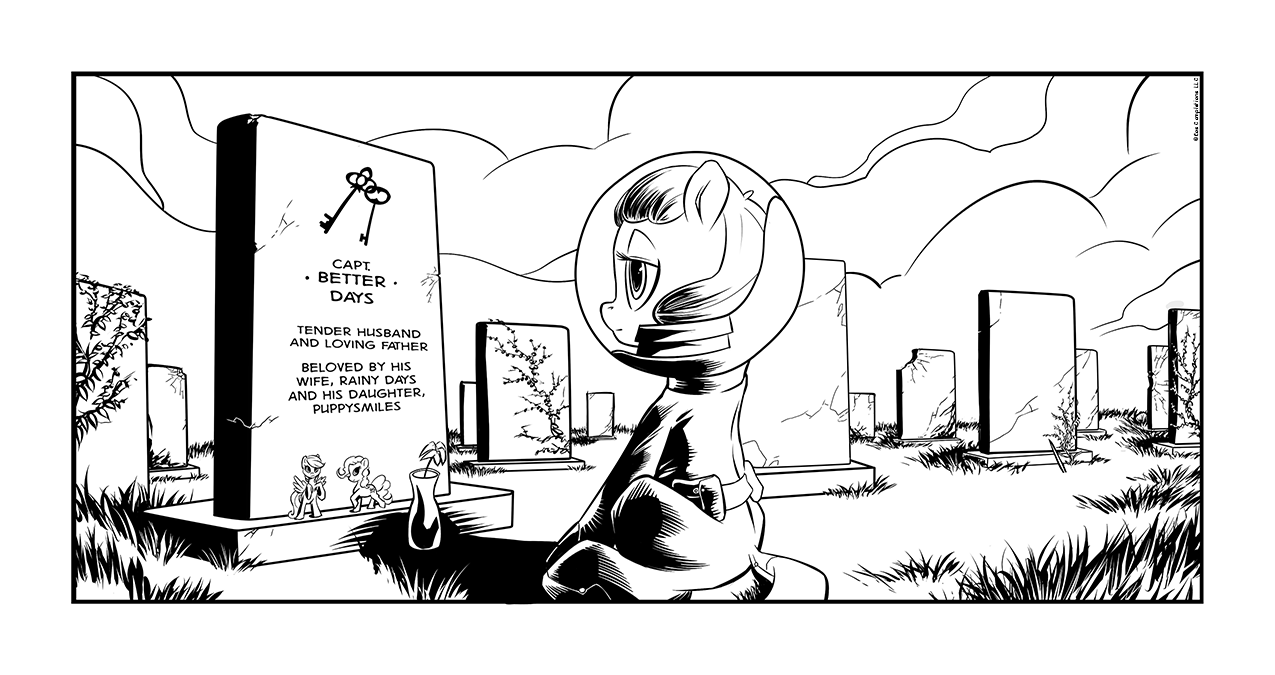
\includegraphics[width=0.9\linewidth]{image16.png}

\begin{intro}
We're getting the band back together
\end{intro}


\rtpr{'Sup, ponies. I can't believe he really did that! He took that piece of crap he calls a rifle and just flew away. That feather head! While I was sleeping! Hey L.P., if you are listening to this, shove that rifle up your ass!}

The radio paused for a moment, the feminine voice that had been talking didn't seem sad or worried, just angry.

\rtpr{All right ponies, the show must go on! DJ Good Stuff here, and you are listening to Radio 52, at least until I collapse because a certain pony left me here all alone with a show that is never supposed to stop! Okay, new rules: I'll be airing during daytime, and you'll get only music during night, because I'm not immortal and I need to sleep. And if anypony wants to drop by and do some talking while I'm asleep, just knock at the door. You know where we are.}

The sound of paper shuffling filled another pause.

\rtpr{All right, remember that I can operate that damn shortwave radio too, so don't stop sending news, especially regarding the situation in Ironworks. And speaking of news, the Memorial has been deserted, and the ponies are moving north, toward Broccoli. All the caravans still moving between Broccoli and Emerald Shores should head north and try to reach Rust Manor. I repeat, head north towards Rust Manor! Don't stop at Broccoli, because it's too near to the war zone.}

\rtpr{Fuck, I hate giving the news. If anything else comes in I'll let you know, otherwise you'll get music all day long. Remember, music means no news and no news is actually good news. Have some angry music because I'm angry and give Lonesome a buck in the head if you see him.}

\begin{music}
		Say your prayers, little one,
	
		Don't forget, my son,
	
		To include every pone.
	
		Tuck you in, warm within,
	
		Keep you free from sin,
	
		`til the sandmare she comes
\end{music}

\horizonline

% NOTE: force to break line
% \englishdaytimeplace{13}{4:00 A.M.}{The Memorial northern picnic area, Big 52 S Branch}
\englishdaytimeplace{13}{4:00 A.M.}{The Memorial northern picnic area,\\ Big 52 S Branch}

In the distance, far ahead of Puppysmiles, stood another little town, little more than a group of shacks built around a very large statue that depicted a group of ponies hoisting an Equestrian banner. The marble monument was remarkably well conserved, and its enormous size made it possible to see even from several kilometers away. On her way south, she met several groups of ponies with carts loaded with everything. She tried to socialize with them, but they simply kept moving, mostly ignoring Puppy except for a couple of foals who waved back from a cart. Entire families were fleeing, leaving their homes and trying to reach safety behind the walls of larger and better guarded settlements.

She was now staring at the monument with a puzzled expression. ``Ah, Mister Voice, are we near to dad's place?''

{\mten ``Analyzing. Actual position is Equestria: Fallen Soldiers Memorial, northern picnic area. Location of your male parent is currently unknown.''}

Puppy tilted her head, studying the surroundings. ``Yes, I remember this place! That big road sign with the Pinkie Pie face and\dots'' She left the road, galloping over a low hill and finding herself in the middle of a group of tables and rusty abandoned barbecues. ``This is dad's place! Dad is near! Let's go!''

Puppy galloped further away from the road, heading for a group of hills to the west. The low hills were still far from here, approximately four or five kilometers away from the Memorial, but even from this distance it was possible to see that they were dotted with white stones, each spaced evenly apart.

As she ran toward the distant hills, Puppy passed by a dead tree. Once upon a time it must have been a proud oak, but all that was left now was just a blackened skeleton, its trunk scorched and its branches bare.

\rcpr{``I want more apple pie!''}

\rcpr{The grass was green and birds were singing among the leaves. The sky was blue and everything was so nice.}

\rcpr{``Don't eat too much Puppy, we still need to go to dad's place, remember? If you eat too much you'll get sleepy, and you don't want to be sleepy when we go visiting Dad, right?''}

\rcpr{``But Mom, he's never there! We went a lot of times and he was always away! Will he be there this time?''}

\rcpr{``I\dots I don't know, Puppy, but you can leave him flowers, so he will find them and know that you love him, okie dokie?''}

\rcpr{A couple of colts chased each other, disappearing behind a hill. There were ponies playing and ponies having lunch. Everypony was having a good time.}

\rcpr{``I got a better thing this time! Look!''}

\rcpr{``Oh, but Puppy, that's a toy of yours! Are you sure you want to leave it here?''}

\rcpr{``Yush! So when Dad will be back he will play with it and won't feel lonely! Besides, he will return it to me when he comes back home again!''}

\rcpr{``\dots''}

\rcpr{The distant sound of laughter filled the silence between mother and daughter.}

\rcpr{``Mom? Why are you crying?''}

She stopped for a moment, looking at the big tree and trotting around it. She could clearly remember having a picnic in this place not earlier than in spring. Where had everything gone? Oh well, she knew that trees sometimes lose their leaves because Mom had told her so and since there wasn't even grass on the ground it was just fitting. She trotted away toward the cemetery.



\horizonline

% NOTE: force to break line
% \englishdaytimeplace{13}{6:00 A.M.}{Interequestrian 52 War Cemetery, Big 52 S Branch}
\englishdaytimeplace{13}{6:00 A.M.}{Interequestrian 52 War Cemetery,\\ Big 52 S Branch}

The tombs were all similar, consisting of small marble stones on which were engraved a name, a date, a cutie mark and a few short words. Some stones were white and other stones were black, but when Puppy asked to her mom why they were different she simply replied that the ponies napping there were more important than the others. Puppy didn't like that reply, since Dad was a very important pony but he only had a white stone; so she decided to bring him some more flowers, just to show him that she was super sure he was the best dad ever.

{\mten ``Warning. Receiving distress radio signal. Distance from the source: two hundred meters. Signal identified: Device 009. Warning. Receiving new distress radio signal. Distance from the source: two hundred and fifty meters. Signal identified: Device 020.''}

Puppy tilted her head, confused. ``Wut? New radio music? I hope it's not like the last time when there was just a stoopid pony saying endlessly `help me, we're doomed' and all those silliness.''

{\mten ``Negative. These are Ministry of Peace distress signals from other MK VI Suits. Receiving a third signal on a distance of two hundred and thirty meters. Signal identified: Device 013.''}

She sighed. ``Look, if it's not music I don't care. Now let's go find Dad, maybe he's back and we will go find Mom together.'' With these words, Puppy headed toward a low hill with the statue of an alicorn on top.

The hill was surrounded by a low fence with several marble arches that led inside that area of the cemetery. A large main battle tank stood in front of the arch Puppy was going through. A brass plaque in front of the war machine explained that in this part of the graveyard were buried the fallen soldiers from the Third Armored Company--Steel Flanks. There were also some commemorative words and a brief statement that explained how tanks nowadays weren't widely used on the front because of the new technological breakthroughs, and that this decommissioned machine had been left here to safeguard its sleeping brothers.

Puppy had been here more than once, so she already knew where to go and headed toward a specific grave. Seeing that the place was deserted, Puppy sighed and sat in front of the white stone.

The cutie mark of a couple of keys was engraved on the marble surface, together with some writing:

\begin{center}
	Captain \quad Better Days

	Tender husband and caring father.

	\medskip

	Beloved by
	
	his wife \quad Rainy
	
	and his daughter \quad Puppysmiles.
\end{center}

% NOTE: Modifine style

The date was mostly unreadable, but it didn't matter very much to Puppy, since she was mostly interested in the grave itself. On the small mound sat an empty vase and a couple of plastic figures. The vase once contained flowers, but now it was just filled with murky water and covered in mold, but the plastic figures still stood on the grave, looking back at Puppy. They were two molded plastic ponies, like those that were put into cereal boxes. The first figure was a miniature Pinkie Pie, while the other was of Rainbow Dash.

Puppy sighed. ``He didn't take them\dots Why does he never takes what I leave here? I was sure that he loved Pinkie Pie and Rainbow Dash!'' Touching the plastic blue pegasus with a hoof, she continued, ``Stoopid Dad; if he was a little more at home, Mommy could be happy\dots''

Oh well, Mom explained plenty of times that it was okay if he didn't come home and that she wasn't mad at him. She wasn't completely convinced, but something in her mother's eyes told her that she just had to accept that explanation. From the day Mom got angry because Puppy didn't want to come home until dad came back with them too, she decided that she didn't want to see her mother cry and scream like that. So she decided to play along and leave something in this place every time she came here, hoping that one day Dad would realize that she and Mom still loved him and maybe he would finally come back.

Puppy cleared her voice and stated, ``Everything.''

{\mten ``Warning. The inventory management spell is not devised to operate more than one object at a time. Opening fast inventory scrolling by alphabetical order. State `next' when you have finished examining an object and need to move on. State `stop' or `exit' when you want to close this application and restore usual inventory management program.''}

An ashtray floated in front of puppy. ``Next!'' Another ashtray appeared. ``Next!'' Yup, ashtray. ``Next!'' Again, an ashtray ``Next!'' Puppy usually scooped up every single shiny object she found on her way, so this was going to take a while.


\horizonline

% NOTE: force to break line
% \englishdaytimeplace{13}{7:00 A.M.}{Interequestrian 52 War Cemetery, Big 52 S Branch}
\englishdaytimeplace{13}{7:00 A.M.}{Interequestrian 52 War Cemetery,\\ Big 52 S Branch}

``Next!'' The twentieth fork was stowed back into Puppy's bags and the sorry, dripping remains of Fuzzy Ball floated in front of the foal. ``Ne---no wait! Fuzzy!'' Grabbing the dead parador cub, a disgusting green goo oozed from the cracks in its carapace. The dead creature had lost all of its legs and only had a single wing left, while the eyes at some point started to decompose and were now just another grossly rotting detail on that thing.

``You don't seem very healthy today, Fuz. What happened?'' Puppy studied the dead creature for a moment, trying and failing to determine what was wrong with it. ``Ah, Mister Voice, is Fuzzy Ball ill?''

{\mten ``Negative. Fuzzy Ball is deceased and in an advanced state of decay.''}

Puppysmiles frowned. She had learned from experience that difficult words usually weren't good news. ``Ah, this means she is very tired?''

{\mten ``Negative. This means she is falling apart. Losing pieces. Disintegrating.''}

``What?'' Puppy cocked her head, alarmed. ``Losing pieces? But Fuz needs her pieces to be okay!'' She gave a second look at the dead critter. ``Besides, it seems to me that she doesn't lack any pieces.''

{\mten ``Advice. Check twice. The creature has lost three wings and all its legs. Moreover, its carapace is rotting and has broken in several places due to the poor condition in which it has been transported.''}

``Transported? You mean that Fuzzy is getting worse because I am taking her along with me? But that's terrible!''

This was a chance that even an automated voice with no real intelligence could be able to exploit.

{\mten ``Affirmative. The corpse is decomposing faster mostly because of you insisting on taking it along. Abandoning the corpse immediately is highly recommended.''}

Puppy hesitated. ``Leaving Fuzzy here? But---but she will be alone! There's nothing here, there's only---'' She stopped talking, looking straight at her father's grave. ``Maybe Dad could take care of her.'' Puppy didn't seem enthusiastic about that idea, still it seemed so obvious.

{\mten ``Elaborating. Leaving a deceased pet in the custody of a deceased parent is\dots Error, cannot compute. Please reformulate.''}

``Reform me late? What are you saying again, you silly voice? I'm trying to being serious here!''

{\mten ``Re-elaborating. It is impossible to identify a logical pattern. An external counselor is strongly advised.''}

Puppy snapped, starting to lose her legendary patience. ``Stop talking nonsense! Call me somepony more competent or we'll end up arguing again!'' She put her hooves on her helmet, as if she was rubbing her head. ''Really, living with you can be a pain sometimes.''

Watcher's staticky voice interrupted the foal-machine quarrel. ``Puppy? What are you doing in this place? It's dangerous!''

Turning toward the voice, Puppy found a spritebot floating to her left, but this time she couldn't smile at him. ``Oh, it's you, Questioner---''

``Watcher\dots''

``---Whatever. This isn't a good moment, could you please come back some other time?''

He hesitated before replying. ``Sure, but I wanted to warn you. This place is not good for you. It's filled with, uh, bad things that you must not see. Please, before I go, promise me that you will get away from here immediately.''

Puppy snorted in frustration. ``I can't. I need help with Fuzzy Ball, but Mister Voice is not helping at all!'' With these words, she showed her dead parador to the spritebot.

``Gah! But that thing is rotting! No please, what is that? Don't tell me! Puppy, throw that thing away!''

``What? But Fuzzy Ball is my very best pet friend! I love her and she loves me and we are having lot of adventures together! I don't want to abandon her\dots'' She hesitated, looking away. ``But\dots''

``But?'' pressed Watcher, since Puppy didn't seem eager to end the sentence and still hugged the corpse.

``But she is ill, and Mister Voice says that she must rest! I could leave her with my dad, but it seems wrong. I didn't even ask him if I could keep her and---''

``Your dad? You know where your dad is and you are still trotting alone through the Wasteland?'' His voice was growing with indignation. ``What kind of a father could ever leave his---'' Watcher stopped abruptly, finally noticing the name on the grave that Puppy was sitting in front of. ``Oh\dots This keeps getting better\dots''

She went on, ``I know that I should have asked before taking a pet with me but, but\dots'' She sobbed. ``But I only wanted a friend to stay with me all the time! Not a weird voice that always tells me what to do, or a stoopid chicken that comes and goes! Fuzzy never leaves me alone and keeps me company! We were having lot of fun together and I protected her from the pet eaters and she never goes away and\dots''

Puppy paused, looking at the spritebot. ``And now she is ill and she loses pieces! Mister Voice says she has less wings than before. I'm not good with numbers, but it seems that he's right! I don't want to leave her, but I don't want her to be ill because of me. I don't know what to do!''

``Ah, and what did Mister Voice say?''

Puppy snorted. ``Nothing! He is talking nonsense since I started asking him! Then I had this idea of letting Fuzzy stay here with Dad to see if she gets better, but I don't know if Dad will like her or if he will be angry and, well, I'm not sure Dad will come here, because he is never here when I come, and even if Mom says he loves me, I can't figure why he always avoids me!'' She waved her hooves around, as if she couldn't stand still while she was expressing her concern. ``So maybe he will hate Fuzzy Ball and then she will be sad, but I can't take her with me because she's losing pieces, and losing pieces is bad!''

Watcher hesitated, trying hard to disentangle the knot of feelings and words that Puppy was bombarding him with. ``Well, um, what if I take Fuzzy with me? Just put her into this spritebot's cargo bay and I'll take care of the rest! Sound fair?''

Puppy tilted her head. ``You will make Fuz feel better? Really?''

``Sure, she can't get any worse anyway. I'll see what I can do, but now please, get away from this place, it's not good for you.'' With these words, a hatch opened on the spritebot's side, revealing a space large enough to house the dead critter.

She looked at the metallic stash, then at Fuzzy Ball and sighed. Hugging her pet one last time, she whispered her goodbye. ``Don't worry, Questioner is a pretty pony. When you get better we will play again together.'' Kissing Fuz goodbye through the helmet's glass, Puppy put the dead creature inside the spritebot, the hatch closing almost immediately.

``Don't worry about her, little one, she is going to a better place. Now, let's move away from here, it makes me sad, okay?''

She nodded, looking at her father's grave. ``Lily.'' A plastic flower floated in front of her and she put it on the ground before the marble stone. ``Sorry Dad, I have to go. But next time I'll stay a little more, okie dokie? I'll come here with Mom.'' Turning away from the grave, Puppy smiled at the spritebot. ``All right, I'm done.''

There was a pause before Watcher spoke again. ``You're a good filly, Puppy.''

Puppy and Watcher moved off along the road that headed away from the cemetery, towards the Memorial. The ponies on the large statue seemed to salute the fallen from across the distance, like an eternal link from those who had died fighting and those who were left, trying to win a war that in the end killed everypony.



\horizonline

\englishdaytimeplace{13}{7:15 A.M.}{The Memorial, Big 52 S Branch}

The Memorial was completely empty. While fleeing from the town the inhabitants had taken with them everything that wasn't nailed down and even a few nails that had come loose. By the time two ponies and a sealed crate were flown in by way of griffon, there was only dust and rust left to meet them.

``All right, we're here.'' Mister White jumped down from the griffon that was transporting him and stretched his legs. ``That was a long trip.'' He tipped his black hat. ``You lot can go back to Sun City.''

The first mercenary griffon nodded to him. ``Okay, boss, but are you sure you want us to leave?''

He snickered, looking at the other pony as he disembarked clumsily. ``Absolutely. This is family business, we just needed to get here fast, now your work is done.'' The griffon's expression was still uncertain. ``Oh, don't worry about your pay. If I don't come back, my son will take care of the company.''

The griffon shrugged and waved at the others. ``Okay, you heard the boss! Let's get out of here, lazy feathers!'' All three creatures took off the ground and headed north.

While Mister White watched the griffons flying away, Sage Brush dragged the heavy crate inside a small shack made of plastic sheets and large road signs, complaining all the way. ``We can't take all this stuff with us, Uncle White, it's too heavy!''

``Don't worry Sage, I'm planning to make camp here and then move fast, scouting the area. She can't be very far.''

``I still can't see why you decided to run all the way out there with just me for company when we could simply call the guys.''

``First of all, we had to get here fast and we can't airlift all those ponies and equipment in time. Moreover, Rust Manor is paying good caps for our mercenaries, and I don't see why we should lose earnings.'' Mister White tapped his chin, trying to find something else to add. ``Besides, we aren't going to face the Wild Herd; we will just get the foal and head back, easy peasy.''

Sage Brush sighed. ``Did anypony ever tell you that you're weird? I know she saved our rumps, but you already gave her a reward for that. I think this foal retrieving mission is suicide.'' He hesitated for a moment, his expression becoming thoughtful. ``Or do you know something I don't?''

Mister White enveloped a pair of binoculars with his telekinesis and scouted the surrounding hilltops. ``Well, let's just say that I asked some questions here and there and it seems that wherever that foal goes, things change for the better. This `ghost' must have some sort of lucky star watching over her, and I want to be there when the filly strikes again. There's a lot to gain from this story.''

Sage Brush waved a hoof, dubiously. ``And you say this because?''

``\dots Because I have a good feeling about it.''

Sage facehoofed. ``Great, so we are following a ghost because you have a doozy! Why am I coming with you?''

Mister White replied merrily, ``Well, because I'm your dear uncle and you owe me so many caps that you can't say no anyway.''

``I hate my life,'' groaned Sage Brush.

Mister White waved a hoof, asking for silence. ``Shut up! Somepony is coming from the hills, get the rifle.''

From their improvised sniping position, the two ponies observed the solitary figure trotting in town. It was covered in a dusty mantle and carried a long carbine on its back. The traveler's face was hidden under a hood, but from its neck hung a necklace of feathers and polished metal objects.

Sage Brush lowered his rifle, sighing in relief. ``Meh, it's just a farseer. Weird, what's a shaman doing this far from the desert?''

Mister White trotted out from the shack, leaving his rifle behind. ``We'll find that out soon.'' He galloped toward the newcomer and called out to him or her. ``Hey you! This place is empty. The road heading south is dangerous! You should turn your tail south and head north!''

The hooded pony stood for a moment, looking directly at Mister White before taking off her hood, revealing the face of an old unicorn mare. ``Oh, you are already here. Very well, now we have to wait for the others.''



\horizonline

\englishdaytimeplace{13}{7:30 A.M.}{The Memorial outskirts, Big 52 S Branch}

``So, Puppy, you never told me about that blue streak in your mane. How did you get it?'' The spritebot floated alongside Puppy as they slowly made their way from the cemetery and towards the Memorial. The graveyard gates were just a few hundred meters behind them.

``Ah, it was in Sun City, when Blue Voice told me all those meanie things. I don't remember very well, but at some point I went to sleep and when I woke up my mane was all fancy.''

``I see. You went to sleep, and woke up with your mane changed\dots and what did Mister Blue tell you?''

Puppy sighed. ``I already told you that! He said I was a robot and wanted to make a fool out of me, but I showed him that I was smarter. But that's an old story, since now we are friends.''

``Beg your pardon? You are friends now? Didn't you kill him with a mag pulse shell?''

Puppy giggled. ``Of course not, you silly Questioner! He is not a bullybot! He's just as stoopid as a colt! But when we met again and Creepy Voice bullied him, he said he was sorry so even if he pretends to be grumpy I know we're friends!''

``Creepy who now?'' The tiniest shadow of concern started dancing in Watcher's voice.

Puppy tapped at her helmet. ``You know, Creepy Voice! The one who lives in my head, talks weird and does a lot of cool stuff, but is a jerk?''

After a long pause, the spritebot replied. ``You mean Mister Voice, right?''

``Ah, nope. Mister Voice is a bit boring and talks nonsense, Creepy Voice is creepy but cool. She does stuff like opening doors and spanking bullybots.''

From the robot's speaker came a gasping sound. ``Ah, now I get it! It's an imaginary friend! Yeah, I remember something like that. Want some advice? Don't try blaming your friends for things you did. In the end it turns against you.''

Puppy tilted her head, a little confused. ``She didn't seem very imaginary. Ah, okie dokie?''

``Good filly, you always make me---''

\emph{BOOM!}

Watcher disappeared in a blaze of fire, right in front of Puppy's eyes.

She stepped back for a moment, trying to understand what was going on, then she noticed a large, squat metallic figure rolling over the top of a nearby hill and suddenly she knew the answer. ``Bullybots\dots''



\horizonline

\englishdaytimeplace{13}{8:00 A.M.}{The Memorial, Big 52 S Branch}

Mister White sat at a table inside the shack while Sage Brush finished cooking the oatmeal. ``All right, Long Ears, so when are these others ponies supposed to arrive?''

She shrugged, continuing to look outside the window. ``We should move by tomorrow evening. Many are coming, so much blood\dots''

Brush turned towards the farseer. ``Hey, old hag, we aren't going to fight! We're just here to get that foal and go back to Downtown. I don't care about your crazy visions.''

White waved a hoof at his nephew in an attempt to make him be quiet. ``Ah, you do the cooking, I do the talking. I think we already agreed on that.'' Turning back toward Long Ears, he went on. ``So, what did you see?''

She closed her eyes. ``In my dreams I've seen flames from the south, engulfing all in their path. In the blaze a pink shade kept struggling, the flames danced around her and they seemed to die for a moment as she passed them.'' She paused for a moment before continuing. ``As the fire continued to sweep north, the shade reached the end of the road and turned into darkness.''

Mister White frowned. ``Darkness? What do you mean with that?''

``A black wave that ran behind the fire, devouring it but not before it destroyed everything.'' She sighed. ``And when the darkness devoured the fire, nothing was left. The whole road was just an empty, abandoned place.''

``Well, that's boosting my motivation for sure!'' snapped Sage Brush. ``White, I say we go back to Downtown and leave this fucking place.''

White sighed, shaking his head and ignoring his nephew. ``So, why are we here?''

Long Ears looked away from the window. ``To stop the fire before it destroys everything, and then to reach the end of the road before the pink shadow does.''

``Pink shadow, you say? Why does this makes me think you are referring to Lonesome Pony's ghost?'' He was still talking when a distant explosion got his attention. ``Artillery\dots'' Looking outside the window, Mister White couldn't see any explosion, but it seemed to be quite distant, maybe seven or eight kilometers south east. 

Mister White trotted outside, listening for any more noises, but it was hard to tell if the sound he had heard was actually a distant gunfight or simply his imagination working too hard. ``Well, I guess that whatever it was, now it's gone. Let's get ins---'' A solitary figure was coming from the north, wearing a weathered duster and a leather hat.

He whistled. ``Hey, you! The place is deserted! Go back to Broccoli!'' Again, his voice hesitated when he recognized the newcomer. ``Oh, the old mummy\dots''

Molten Gold quickened his pace and smiled as he approached Mister White. ``Look who's here! White, of all the ponies I expected to meet, you are the last one! What are you doing in this outpost? Checking to see if there's something worth taking?''

He frowned. ``Oh, I'd never steal your job, old mummy. No, we are\dots checking on the situation with the Wild Herd. '' He paused for a moment, trying to read the ghoul's expression, but it wasn't an easy feat. ``So, what are you doing this near to the warzone? Some treasure hunting?''

Molten snickered. ``Something like that. Let's say that I sent a package south without realizing how dangerous it was. Now I'm trying to put a patch on that mistake.''

``This is something new! You being sorry for something! What happened, are you getting old?''

To Mister White's surprise, instead of replying immediately Molten Gold turned his eyes away, looking south. ``Well, yes. But I don't want a kid to die because of me being the usual me. I have a foal to save.''

Slowly, Mister White's expression of surprise changed into an amused smile, until he patted Molten on a shoulder. ``Welcome to the club. Come in, we have oatmeal and a hot mare inside.''



\horizonline

% NOTE: force to break line

\englishdaytimeplace{13}{7:45 A.M.}{The Memorial southern picnic area,\\ Big 52 S Branch}
% \englishdaytimeplace{13}{7:45 A.M.}{The Memorial southern picnic area, Big 52 S Branch}

Puppy galloped toward the big robot, with \emph{The Rock Of Destiny} floating at her side. ``Stop breaking my friends you stoopid bullybots!''

On the other side of Puppy's reckless charge stood an old, rusted but functional battle tank, with tracks, turret and everything else. A pony with a spiked mane was poking out of the turret hatch, taking his time as he stared at the solitary foal running toward them.

``Fuck the boss and his orders! Why should we hide in the south when we have a fucking tank! With this little baby we're unstoppable!

``Hey, Gray Matter, the yellow thing is running this way. How about some shooting practice on a moving target?'' With a laugh, the pony retreated inside the tank and closed the hatch. A few seconds later, the turret rotated to aim at the approaching Puppy.

Inside the tank, the pony with the spiked mane was snickering like mad. ``Come here, come here my little pony.''

``No wait!'' A mare with her mane completely cut off put a hoof on the gunner's flank. ``Let's try a different weapon, I want to see this one!''

``Shut up you cu---'' the stallion began scolding the mare, but at the last moment he noticed the big red button she was pointing at. ``Oh, yes! Yes I like it! Let's rocket it to the Moon!''

``You two idiots! Stop wasting time! Less talking, more shooting!'' Snapped the driver, an earth pony stallion.

The gunner snickered. ``Gee, you're such a whiner, Gray! Here, look at this!''

In the meantime, Puppy was a little more than halfway toward her target. Now that the big metal robot was near, she could see it had a large bulky body with a round head and a looooong nose. Oh, it was one of those carts full of teapots! Wait, they weren't bullybots, they were carts!

She stopped for a moment, sitting down and pondering on the nature of that thing. Okie dokie, what did she know? Usually there were ponies on the carts, but she couldn't see anyone on that one. Moreover, it broke Mister Questioner's robot, and this was a typical bullybot thing, so the odds were that it was a bullybot and not a cart, but to be perfectly sure she decided to go and ask.

In that moment, from the top of the tank's turret appeared a trail of white smoke that rocketed toward Puppy at a ludicrous speed. It was like a big funny firework! ``Tee-hee, look! A cloud maker!''

\emph{KABOOM!}

The rocket hit just behind Puppy, sending her flying towards the tank and leaving her in a small heap no more than fifty meters in front of it. Puppy's helmet was gone and the whole suit was peppered with holes. A thick curtain of pink mist was already forming around her while the suit read off its litany of damaged components.

``All right, he's a bullybot.'' Slowly, Puppy got back on her hooves and looked at the large metal monster that now stood in front of her. Her helmet was still missing and through the mist her face was blurry and hard to identify, except for two burning pink eyes that shone in the cloud, making the whole thing glow with an eerie light.

``Yeah! Eat it, yellow whatever!'' The pony with the spiked mane was laughing crazily, when the mare hit him in a flank again, causing him to snap in anger. ``What now, bitch?''

``Hey, Top Gun, I think it's standing up.''

``What the fuck is that? Gray Matter, stomp it!'' All right, the Wasteland was full of weird things and some of them could survive a missile in the face, but being trampled by a tank was a completely different level of overwhelming your enemy. The raider was sure that nothing could live through that.

The tank launched itself onward, aiming for Puppy, who was doing pretty much the same thing just from the opposite direction. When the two adversaries were almost on top of each other, Puppy jumped in the air, grappling the vehicle's frontal plate with her hooves and pedaling in the air with her hind legs.

``It's on the tank! Lucky Charm, go up and shoot it!'' The driver brought the tank to a sudden halt, trying to make her lose her grip, but while Puppy managed to stay holding on, the gunner was thrown forward, bashing his head against the cannon's loading mechanism and knocking him unconscious.

``Don't worry, I'm on it!'' The mare levitated a sub machine gun and opened the hull's frontal hatch, finding herself directly in front of the struggling foal and in the middle of the pink cloud. ``Say goodbye, critter!''

Puppy heard a voice in front of her, something that seemed pony-like, only she couldn't tell for sure. What she immediately recognized was the hail of bullets that pierced her head and her suit in several points, destroying what little of her helmet that had managed to reform. ``Stop it! Stoopid bullybot!''

A new surge of motivation gave Puppy the strength to haul herself completely onto the tank's hull, just to look at a hatch that was rapidly closing again. ``Hey, do you think you can keep me outside? I am Puppysmiles and I go wherever I want!''

She jumped on top of the turret, searching for something to hit with her faithful rock. Thick metal, some more metal, still metal, a glass thing---CRASH!---okay, more metal, an antenna---SDENG SDENG SDENG!---done, a box\dots ``Uh, a box! Okay, get ready for a spanking!'' Puppy loved that line from Creepy Voice, it sounded so cool!

Inside the tank, Lucky Charm was drowning in her own blood after breathing the pink mist, Top Gun was still unconscious and Gray Matter was trying his best to make the mare drink a healing potion. Everypony was simply too busy to worry about Puppy on the tank's roof that was hitting a missile rack with a stone.

This was more or less when Mister White heard the big explosion.



\horizonline

% NOTE: force to break line
% \englishdaytimeplace{13}{9:00 P.M.}{Interequestrian 52 War Cemetery, Big 52 S Branch}
\englishdaytimeplace{13}{9:00 P.M.}{Interequestrian 52 War Cemetery,\\ Big 52 S Branch}

It was much later when three figures approached the grave, not saying a word. All of them wore a MK VI suit, like Puppy's, but the ponies inside were a patchwork of rotting skin and bleached bones. In their burning pink eyes there was no sign of intelligence, nonetheless they stopped to study the hoofprints in front of the marble stone and followed the trail like hounds tracking their prey.


\clearpage

~\vfill

\begin{engnote}
		Level up! (15)
	
		New perk added: Hit the deck - What the fuck!? I was sure I hit her! Your Damage Threshold against explosives is raised by 25; enjoy tossing grenades on your feet.
\end{engnote}



\chapter{Karma}

\chapterintroimage{image17.png}

\begin{intro}
And the whole world has to answer right now 

just to tell you once again. 

WHO'S BAD?
\end{intro}

% NOTE: force to break line

% \englishdaytimeplace{13}{6:45 P.M.}{The Memorial northern picnic area, Big 52 S Branch}
\englishdaytimeplace{13}{6:45 P.M.}{The Memorial northern picnic area,\\ Big 52 S Branch}

A mare and a stallion trotted along the Big 52, both carrying assault rifles. The mare was wearing heavy security barding, while her companion used a mix of various metal plates welded together into what seemed like a bad attempt at making a scene costume for \emph{The Unicorn of Oz} school recital.

``I still don't understand why we can't stay in Tunnel Town. It's way more defensible than everything past the Sugartop---Yeow!''

Trigger Happy hit Jammed Gun on the head. ``Sure, and leave two thirds of the Big 52 in the Herd's hooves! I can't believe you're that selfish or stupid!''

He looked away. ``I'm not selfish, I\dots I'm worried about you. I don't want you to risk your life like this.'' A single glare from her had been enough to make Jamie stop talking for half a minute, but a pony in love is a stubborn pony. ``We should at least stop for the night. The Memorial isn't very far from here.''

``All right, lazy hooves, you win! Geez, do you know that you are a royal pain?'' Trigger Happy groaned. ``Good Stuff said that the town was deserted, but I guess it will offer some better cover than a tent.''

The large monument to the Equestrian Fallen seemed to fade away with the evening light, disappearing right in front of the approaching ponies.



\horizonline

% NOTE: force to break line

% \englishdaytimeplace{13}{7:00 P.M.}{The Memorial southern picnic area, Big 52 S Branch}
\englishdaytimeplace{13}{7:00 P.M.}{The Memorial southern picnic area,\\ Big 52 S Branch}

As soon as the helmet was fully restored, a pink dot appeared in the middle of its display and began to blink.

{\mten ``System successfully rebooted. All functions restored. Diagnostic system is online. Subject 001: Puppysmiles. Female earth pony. Subject deceased, condition stable. All clear.''}

Puppy slowly opened her eyes, still sleepy. First things first, she had to determine where she had awoken. Aw, it wasn't a bad dream. The bare hills and the dead trees were still all around her, and this wasn't her room. Sighing, she got up and tried aligning with the arrow on the compass, but something got her attention.

``Hey, Mister Voice, what's that?''

{\mten ``Analyzing. Tank wreckage. Threat level: none.''}

``Not the bullybot, silly voice!'' Puppy sighed and trotted toward the object of her attention. ``This blinking thing!''

{\mten ``Analyzing. Shortwave portable communicator. Researching frequency. Decrypting code. New communication channel detected. Receiving call.''}

``Yay! A phone call! Let me take it please please please! I love answering the phone!'' Puppy cleared her voice. ``A-hem! Hullo pretty pony, this is me, Mom is not at home!''

A surprised and angry feminine voice came from the other side of the call. ``And who the fuck are you? Where is Lucky Charm?''

Yay, guessing game! ``Hi, I'm Puppysmiles! Who is Lucky Charm? I know a pony named Lucky Strike, is that okay?''

The communication was interrupted abruptly, leaving Puppy a little stumped. ``Aw stoopid phone pranks! Oh well, don't get angry, or they will win the game.'' Puppy shrugged and trotted away.

{\mten ``Attention, incoming call. Opening communication.''}

Without even giving Puppy the time to reply, the same voice from before started talking rapidly. ``Okay listen up fuckers, I think this frequency isn't safe anymore, but the boss is going to fuck me hard if you don't turn that fucking tank south and bring your fucked, drug filled asses back right now, got it Lucky? I'll repeat that: tell Gray and Bleeding to take that tank back RIGHT NOW! This is the last time I'm asking politely!''

``Tee-hee, pretty pony says funny words!'' Puppy giggled. If this was a phone prank, it was fun.

``What the---you again? FUCK!'' The communication closed for the second time.

Puppy tilted her head. ``That was weird. Maybe we should go away?''

{\mten ``Affirmative. Primary objective is not in this location. Attention, incoming call. Opening communication.''}

The same voice as before started talking again. ``Lucky Charm, Lucky Charm, this is Pony Fort, come in!''

Puppy smiled. ``Nope, but I hear you! Is it okay?''

The mysterious voice sighed, giving up. ``Listen, kid, I have no idea who you are, but I am trying to find some ponies and your radio is causing interference; how are you broadcasting on this frequency, anyway? Where did you get the channel encryption code?''

``What? A code? I know it! It's Puppysmiles!'' she replied.

``Damn kid, turn off your radio, I'm trying to get in contact with a bunch of worthless Dash-heads! Unless you have seen a tank roaming free in the wastelands, you are of no help at all.''

Puppy tapped her helmet, trying to focus. ``A tank, uh? What does it look like?''

``Are\dots are you serious? It's big, rusty, has a turret with a big gun, and moves on tracks.'' The voice paused for a moment, hesitating. ``Have you seen it?''

Puppy looked at the still smoking carcass of the behemoth lying not far from her. ``Ah, does it go bang and boom and toss exploding things?''

``Yep, that's it! So, have you seen it?''

``Uh-uh.'' Puppy nodded. ``But it was being a bully, so I hit it with my rock and it exploded.''

There was a long pause from the other side of the call before the mare replied with a dismissive tone. ``Yeah, sure, now go and fuck yourself with a cactus.'' The call was interrupted again.

Puppy shrugged, this new voice was being very odd. Nonetheless, she had an arrow to follow and a lot of road to scoot, so she had no time for prank calls. Still, when was she going to have another chance to prank call a prank caller?

``Ah, Mister Voice, can you call Pony Fort, pretty please?''

{\mten ``Affirmative. Opening connection.''}

The female voice from before replied almost instantly. ``Pony Fort here, I copy you, speak.''

``Ah,---\emph{giggle}---I am looking for---giggle---Mister Ai Em---\emph{giggle}---Ai Em Stew Peed---\emph{giggle}---'' Puppy couldn't help but laugh---this was a prank she had seen once in \emph{The Foalsons.} She'd always always \emph{always} wanted to try it out.

There was a long silence before Pony Fort replied. ``Really? A prank call? Look, I'm going to find this Mister Stupid, and then he'll come there and spank you so hard that your tail will be sticking out your forehead!''

Puppy gasped. ``NO! No please I'm sorry! Don't spank me! I'll behave!''

The mare laughed for a while before replying. ``Too late, little prankster! Watch your sorry flank because he's already coming for you!''

``EEEEEEEK!''

She launched herself in a run through the hills, fleeing from the incoming spanker and disappearing behind a hill. Run Yellow Prankster, run!



\horizonline

% NOTE: force to breakline
% \englishdaytimeplace{13}{7:30 P.M.}{The Memorial northern picnic area, Big 52 S Branch}
\englishdaytimeplace{13}{7:30 P.M.}{The Memorial northern picnic area,\\ Big 52 S Branch}

Not too low, not too high, and especially don't let your enthusiasm drive you, old pegasus.

Lonesome Pony was flying above the hills, looking for some landmark to navigate by, but past Broccoli the night had begun to fall, and now it was hard to see anything.

``Damn, I'll have to land for the night if I don't want to fly straight into some raider patrol.'' Sighing, he landed on a barren hill and finally stretched his wings in relief. ``All right, let's check where I am.''

He had kept his PipBuck receiver tuned to Radio 52 on a very low volume the whole time, but when the music stopped and Good Stuff began talking, he stopped checking the map in order to listen to the news.

\rtpr{``Okay, my little ponies, this is Radio 52 and I am DJ Good Stuff\dots Just, this time there's nothing good.''}

DJ Good Stuff sighed; she seemed on the verge of tears.

\rtpr{``Ironworks is no more. I received a communication minutes ago. The Herd opened a breach in the factory, and the surviving defenders retreated inside the city Stable. The Herd seems to have better weapons, better robots, better everything. Approximately two hundred ponies, mostly foals and mares, are now separated from a blood craving horde of raiders by a Stable door.}''

She paused again for several seconds before continuing.

\rtpr{``I\dots I don't know what to say. The Hired Hooves are reinforcing the Rust Manor garrison and won't move a hoof, but if nopony does something, then all those ponies at Ironworks are doomed. They sent a last message desperately pleading for help, begging somepony to save at least their foals.''}

Lonesome Pony sighed, shaking his head. ``Goodie, this way you're helping nopony! I can't believe that the only thing you can do in a moment like this is whine like a foal! Ponies need a voice to guide them, not\dots not this!''

He turned his head north, hesitating. ``Why must I do everything by myself?''

\rtpr{``Ah, sorry ponies, I'm not used to this and, well, I guess it's not my problems we are discussing here, but I think that things can still turn for the better. Those ponies in Ironworks are alive and a Stable door is not that easy to open, so\dots think about this. Next time it could be you. Thinking that you're safe just because you are elsewhere doesn't work at all, since the Big 52 is all the same place. If Ironworks dies, then Broccoli will die next, and Rust Manor. The Herd will be unstoppable if we let them take a running start.''}

Lonesome raised an eyebrow and closed his wings, listening to her voice. Good Stuff was becoming more and more confident, as if she finally found the thread of her speech and now she seemed to know where to take it.

\rtpr{``But if we stay together and face them before they become unstoppable, if we go to Ironworks and save the lives of those innocents, well, I think that we can still win. The only thing we need is to stick together and face the enemy as one. Lonesome Pony is already flying there; you just have to follow his example and show those mules their place!''}

``Not bad. There's a lot of room for improvement, but at least she didn't tell them to run as far as possible.'' He sighed in relief. ``All right, maybe I didn't make a mistake leaving her alone.''

\rtpr{``But I'm talking way too much. This is a radio and there should be music playing, so this is for you, Ironworks. Don't give up, somepony is coming! Hold on my little ponies! Just believe in each other. You gotta believe.''}

\begin{music}
		If just one pony believes in you,
	
		Deep enough and strong enough, believes in you,
	
		Hard enough and long enough, before you knew it,
	
		Somepony would think, if he can do it, I can do it,
	
		Making it two,
	
		Two whole ponies believe in you.
\end{music}

Lonesome snickered, hearing the song. ``Good choice. Maybe a little childish, but it's foals we're trying to save. I just hope those mules will get it, or this is going to be the shortest counterstrike ever.'' He smiled a little and trotted away, toward the Memorial.


\horizonline

\englishdaytimeplace{13}{9:00 P.M.}{Wastelands, Big 52 S Branch}

The five raiders were a little bit stumped. Not only was a foal not supposed to run at them asking for help, but ponies were supposed to die when you shot them repeatedly in the chest. Apparently nopony had informed this one.

``Oh please please please, hide me! He's coming and I has nowhere to run! Please please PLEASE!'' Puppy stomped her hooves on the ground. ``I said I was sorry, but he didn't care!''

A large earth pony stallion with a scar along his neck approached the foal, while the other four ponies kept their weapons pointed at her. ``Who the fuck are you? What the fuck are you? Who the fuck is after you? And why the fuck are you still alive?'' The pony noticed that the holes in the foal's suit were already disappearing and that she hadn't shown the slightest sign of being in pain. All right, maybe listening to what this creepy foal had to say was a good idea, after all.

``Ah, I'm---'' Puppy stopped abruptly. What if one of these ponies was Mister Stoopid? She had to play smart. ``I am, uh, a ghost! Yush, I totally am the ghost the voice in the radio always talks about, and, ah, my name is absolutely not Puppysmiles.'' From the look the ponies gave her, Puppy felt she had to add something. ``Ah, nopony here is called Mister Stoopid, right?''

The stallion nodded slowly. Pink gleaming eyes, a yellow containment suit, ignoring gunshots\dots Yes, that matched with what he heard about the Ghost pretty well. ``So, you're the Ghost of the Big 52.''

``Yup.'' Puppy nodded. Now that her master skill at lying was being tested, she had to be strong, she had to be firm, she had to be smart. Show your best poker face, Puppy!

``And your name is\dots Not Puppysmiles?''

``Right.'' It was working! They were falling for it! Cunning Puppy, master of deceiving!

``The Ghost of the Big 52, sentry bot killer and town rescuer? That ghost?'' The other ponies behind the leader took a step back. They seemed afraid of her.

``Yes I am!'' Puppy nodded vigorously.

``And you want help from us.'' The stallion seemed a bit confused.

``Yush! Well, that is, if nopony's name here is Mister Stoopid.''

``I\dots no, my name is Slash Blade, the unicorn there is Collateral Damage and his bitch is Paper Cut. Then we have Stinky Tail and Plastic Flower.'' He pointed at the last two mares in the group while speaking their names. Besides Collateral Damage and Paper Cut, all the others were earth ponies.

Puppysmiles sighed in relief. ``Whew, that was close! Listen up, there's this mad pony following me. He's super angry because I made a prank call to him and nao he wants to spank me! Can I, ah, hang with you for a bit? So you can tell him I'm a nice pony and he'll go away. Puppy please?''

Blade looked back at his companions. The other stallion shrugged, while the three mares didn't seem eager to help. ``Are you really fleeing from a pony because you played a prank on him and now he wants to spank you?'' This was getting weird.

She nodded.

He raised an eyebrow. ``Are you retarded?''

``Ah, mmmaybe? Will you help me if I say I am?''

Slash sighed again; he was sighing a lot, lately. ``You're going to follow us anyway, aren't you?''

Puppy nodded again, smiling.



\horizonline

\englishdaytimeplace{13}{10:00 P.M.}{The Memorial, Big 52 S Branch}

Mister White smiled as he floated the canteen back into his saddlebags. ``So, you ditched the radio and flew all the way here because of a pony you haven't even met?'' The unicorn snickered.

``Sort of. I had a feeling that the wind was changing and, well, I just wanted to be there when it happened. Actually, I was surprised to find you here.'' replied Lonesome, looking at the group of ponies in the shack.

So far there was a farseer from the Sand Sweepers, the Security head mare of Tunnel Town with her\dots henchpony? Coltfriend? Doesn't matter. The most infamous grave robber in all of Equestria, and Mister White with his nephew.

``So, what's the big plan?'' Lonesome looked out into the night, waiting for a reply that came from the farseer.

``We're still waiting for friends. Tomorrow we act. Now the fire is burning too brightly. We need to wait for the flame to flicker and then make our move.'' Long Ears closed her eyes, breathing deeply.

``Look, I don't care very much about this whole prophecy thing,'' interrupted Trigger Happy. ``I just want to know if Puppy is all right. Can you tell me that, you Mint-als sink?''

Long Ears opened her eyes, shrugging. ``And how am I supposed to know that? The visions come to me, not the other way around.''

Happy didn't reply. Instead she turned her attention to the ghoul sitting in the corner. Molten Gold hadn't spit out a single word since she and Jamie arrived in town, but he seemed troubled. ``So, old mummy. You should come north more often.'' She tried smiling at him. She didn't like him, but he hadn't actually done anything to deserve her mistrust. Yet, at least. ``I'm curious, what did that filly do for you?''

He slowly turned his head toward the guard chief. ``It's not a matter of what she did for me, it's what I didn't do for her.'' Molten snickered; it was a raspy and unsettling sound. ``For the first time in two centuries I feel guilty. Can you believe that?''

Sage Brush sighed. This seemed to be the ``tell your story'' moment of their ``oh-so-pretty'' slumber party. ``Spit it out. Most of us will be dead before this little adventure ends anyway. It's not like your secret is going anywhere.'' He chuckled before continuing. ``Then we should tell each other creepy tales and have a pillow fight. Isn't it a great idea?''

Mister White facehoofed. ``Sage, please, shut up.''

Molten shrugged. ``It's not a real story anyway. I just happen to have known Puppy's mother, Rainy Days.'' Molten Gold was speaking slowly, with a distant voice. ``She was some sort of local hero. Nothing special, but in those days when everypony was scared and confused, she had the resolve to organize a refugee camp and helped a lot of ponies.'' Shaking his head, he corrected himself. ``Well, mostly she showed other ponies how to help themselves, then moved on to the next town and did the same thing from the scraps, teaching ponies how to survive.''

Jamie interrupted him. ``Wait a single fucking second. You knew Puppy's mom, and then you met Puppy. What did you tell her?''

Molten Gold looked straight into the guard's eyes. ``What could I have told her? `Sorry but your mom is dead?' Have you looked her in the eyes? I sent her to Ivory Tower, hoping that the rangers would find a way to\dots'' He hesitated, turning his head away. ``To help her.''

Nopony replied for a moment, not until Trigger Happy realized the meaning of Molten's words. ``Hey, but Ivory Tower was completely destroyed! You sent the foal there?'' She retrieved her combat rifle. ``You fucking son of a b---''

Jamie and Lonesome Pony jumped on Trigger Happy, immobilizing her. ``Woah, Happy, calm down! She was sighted in Broccoli, remember? She's fine!''

Molten sighed, shaking his head. ``Well yes, she should be fine. The funny thing is that even most of the ponies living in Ivory Tower are fine. They just lost their playground.'' He smiled. ``I wouldn't be surprised if somepony told me that the filly did that.''

Lonesome Pony let Happy go and got himself back on his hooves. ``The two slaves she freed told me that she was like a ghost. Bullets passed through her as if she wasn't even real, and her gleaming pink eyes turned the slavers against each other.'' He weighed his next words carefully before speaking. ``Do you believe in ghosts?''

``Oh please!'' snapped Trigger Happy. ``Don't even get me started on that! This idiot,'' She pointed at Jammed. ``has asked that ever since Puppy arrived in Tunnel Town. Okay, the foal is not a common pony and I'm not sure she is even a ghoul, but I hugged her and she is more than solid.''

White looked outside the window. ``I think we should speculate a little less and keep an eye on the outside a little more. There are several ponies approaching from the north.''

All the eyes in the room turned toward Long Ears, waiting for a response. The farseer smiled when she got up and walked to the door. ``They arrived early. Very well, let's go and meet these famed Applejack's Rangers.''



\horizonline

\englishdaytimeplace{13}{10:30 P.M.}{Wastelands, Big 52 S Branch}

A small fire burned in the middle of the haphazard camp. The two earth pony mares were cooking some canned food while the other cleaned guns. Every pony tried to ignore Puppy.

Stinky Tail was chatting with Collateral Damage, ignoring the glares of jealousy from Paper Cut. ``So, do you think they already opened the Stable?''

The unicorn shrugged, keeping his eyes on the firing mechanism of his weapon. ``It's just a matter of time. Those fat bastards won't find mercy after making us starve for years.''  Collateral spat in the fire. ``We lost seven last season because of dirty fucking water. I just hope I'm there when we get in.''

Plastic Flower snickered. ``Those fuckers have all the good land and they've hoarded all the good stuff from this shit hole. Well, not anymore! This time we win!''

Slash Blade nodded thoughtfully. ``And we'll make sure that they won't come back. Ever. Ironworks, Rust Manor, Salt Cube\dots Everything will burn.''

Puppy wasn't really listening to the ponies, being more interested in the way they worked around their weapons. It seemed plain stoopid; there were better ways to clean something. ``So, that is how you keep clean your noisy thing? Why don't you wash it? It's easier.''

Along the trail Puppy had been a constant pain, an endless torrent of words. The raiders tried scolding her and shooting her, but nothing seemed to work; she simply kept chatting and chatting and blah blah blah. The only thing that worked to keep her at bay had been the threat of spanking, but nopony was really willing to get physical on a thing that ignored bullet holes in her chest. Besides, the pink gas that poured from those holes seemed dangerous, and even more creepily, it seemed alive.

``The gun needs to be oiled, unless you want it to jam and explode in your mouth,'' Paper Cut explained. ``Didn't you ever fix anything?''

``Sure! I fix a lot of things! I'm the best fixer ever!''

``Fix things? Like what, brains?'' The unicorn mare laughed.

``Nope, I fixed a radio, then another radio and then, um, a big screen, and I made my voice friends working again and they were super happy. Ah, I'm a voice fixer, I guess?''

Paper interrupted her work, now staring at the foal. ``You can fix electronics? Really?''

It was now or never. Puppy wanted to impress these pretty ponies so that they would be her friends, and maybe they were going to help her if Mister Stoopid came to spank her, and then maybe they were going to help her find Mom, too! ``Sure! I can fix anything!''

The unicorn floated a radio receiver in front of Puppy. ``Prove it. This radio stopped working this afternoon; since then we have been cut off from our base. Repair it and you'll officially be a member of the Wild Herd.''

She looked at the radio and giggled. ``Ah! Last time it was a whole room filled with these things! Easy peasy!''

\emph{WHACK! WHACK! WHACK!}

Puppy struck the ground with the radio until it cracked open. Then she gave a long look inside it before nodding knowingly. ``Yeah, sure, it's really easy: it's broken.''

The unicorn facehoofed and moved toward Puppy to retrieve her now even-more-broken-than-before radio, but Puppy wasn't finished.

``Nao all I need is to put some pretty stuff inside it.'' Puppy grabbed an energy cell and stuffed it into the poor radio, then hit it again a couple times for good measure. Cracking and fizzling, the communicator came back to life.

The mare grabbed the radio from Puppy's hooves and activated it. ``What the---you fixed it!'' She immediately tried contacting the base. ``Red Roach standing by. Come in Pony Fort, over. Red Roach standing by. Come in Pony Fort, over\dots oh, c'mon!''

All the raiders stopped their activities for a moment, listening to the mare talking in the radio and waiting for a reply.

The communicator crackled and spat sparks from its new battery, and with sparks came words. ``This is Pony Fort, where the fuck have you been, Red Roach? We were already going to sell your stuff away!''

While the conversation between Paper Cut and the raider base continued, the other ponies celebrated by shooting into the air and hitting each other on the back. Puppy giggled a bit, looking at the weird scene until Slash Blade approached her, patting the foal on the helmet.

``Well done, little one! Who knew that you were such an electronic genius? We completely underestimated you. Welcome to the Herd.'' The raider was going to say something more, but his attention was caught by Paper Cut's expression when the mare closed the communication.

``Gray Matter didn't return with the tank. The boss wants us to head back to Ironworks as soon as possible.''

Plastic Flower shook her head. ``Those idiots ran away with the tank. I told the boss not to give them too much firepower. Those fuckers have never given a fuck about the Herd. They only wanted to set the Big 52 on fire.''

``Aw, who cares?'' added Stinky Tail. ``We got other tanks, and the robots. We are unstoppable this time!''

Collateral approached Puppy, putting a hoof on her back. ``So, little ghost, are you ready to see our base?''

``Ah, I don't know. I should go looking for my mom. She's somewhere in that direction.'' Puppy pointed south.

``That's fantastic! It's exactly where we are going!'' Slash patted the foal on the helmet again. Everypony here was a patting pony. Puppy could live with that as long as they didn't spank her.

The raider leader continued. ``Okay my dirty ponies, we don't sleep tonight. We'll have to trot all night long if we want to reach Ironworks before morning's light.''



\horizonline

\englishdaytimeplace{13}{11:00 P.M.}{The Memorial, Big 52 S Branch}

Scold sipped his tea, looking at the lights in the other houses. With a deep sigh, he turned on his tail and looked at the other ponies in the room. ``Very well, so we have a DJ, a ghoul, a merchant, a drug addict and three guards?'' He shook his head. ``I was expecting something more from the Big 52, at least from the Hired Hooves.''

Cold Shower shrugged. Without her armor she was quite small, even for a mare. ``I don't care. We have our own troops, and these ponies are just some more firepower I didn't even expect to get.''

``Well, they are also the ponies that we Applejack's Rangers are trying to protect, aren't they?''

She frowned, dismissing the scribe's words. ``Actually, I don't see any helpless foals in this place. For all I know, they're just volunteers fighting for their homeland. If they want to tag along I won't tell them to go away, but---'' A knocking on the door interrupted their discussion. ``Yes, come in.''

When the door opened, Mister White made his way into the room. ``Good evening, scribe Scold, Paladin Shower.'' He paused, looking at the two for a second before continuing. ``Is everything all right?''

Scold turned toward Mister White, studying him. ``Oh, look, the leader of the most powerful tribe along the Big 52. May I ask why you only brought along one soldier?'' Scold paused. ``Or are reinforcements on their way?''

White shook his head. ``Nope. I'm not here as the head of the White Apples or the Hired Hooves. This is a very personal affair. I'm paying back a debt while hunting for opportunities.''

Cold Shower muttered something that sounded a lot like ``Fucking blood sucker,'' but if White heard her, he didn't react.

Scold moved toward him and raised his voice, trying to draw away as much attention as he could from the not-very-diplomatic mare. ``A debt? Let me guess. The ghost?''

``Wow, your skills have improved since last we met, or does the elder scribe cape come with a `detect obvious' spell?'' Mister White snickered. ``I'm just kidding, no offence meant, but everypony here seems to have been lured by that foal.''

``Indeed. It's incredible how much a single reminder of what we were could move so many hearts. I would be a liar if I said that I'm here just for the Applejack's Rangers oath. I want to be there when the foal reaches the end of the Route.'' He smiled slightly. ``But I don't think you're here to talk about ghosts, are you?''

Mister White laughed for a moment before replying. ``Well, that was a reason, but there's something else. I am a pony of many interests, after all. I wanted to know if there is a way we could help the Rangers in the upcoming battle.''

``Upcoming battle? That's interesting. And if I may ask, what battle are you referring to?''

He snickered. ``All right, let's play your game. You're going to hit the raiders while they're still occupied with Ironworks' Stable. That seemed pretty obvious to me, since it was what I would do.''

Scold nodded. ``Yes, it's pretty obvious, but I don't think that we will get a better chance to strike unless we forfeit Broccoli, Rust Manor and Sun City.'' Scold turned his head toward Cold Shower. ``But I am the wrong pony to ask, if it comes to strategies. Paladin, do you have anything to say?''

She sighed, clearly annoyed by the fact that Scold had involved her in the conversation. ``I don't know what we'll find in Ironworks, but the plan is to break through the enemy lines and reach the Stable, secure the area and then evacuate the civilians. The more you can help, the better.''

White nodded, slowly. ``I heard they have robots and armored carts. Maybe we should study a better plan than simply rushing in and getting surrounded and overwhelmed by their superior firepower?''

Scold rose a hoof. ``No, wait, you are misunderstanding. The rangers will break through the lines. You'll wait outside, covering our retreat.''

``Oh, wonderful, a suicide plan where I'm not in the suicide lot. I already love it.'' Mister White put all the sarcasm he could in his voice. ``And what will we do when this `they'll never know what hit them' plan utterly fails?''

Scold shrugged. ``Don't worry, I've got a backup plan; the Rangers will deal with the Wild Herd, even if we have to bring down the sky.''



\horizonline

\englishdaytimeplace{13}{11:30 P.M.}{The Memorial, Big 52 S Branch}

Molten Gold was sitting outside the town's barricade, looking south while smoking a cigarette. He coughed badly, snickering by himself, when Trigger Happy arrived and sat on his left.

``So, you met her mom\dots'' Her voice was distant, thoughtful.

He nodded. ``Yup. She bucked me out of town when I tried to steal some Rad-X. I used a lot of it since I was scavenging irradiated zones.''

``Let me guess. You kept scavenging without the Rad-X?''

He snickered again. It was an unsettling sound, like the rattle of a dying pony. ``Wow, you must be some sort of scholar. I always blamed the bitch for doing this to me, but in the end I always knew it was my fault. Oh well, I'm still alive to tell the story, at least.''

Happy hesitated before asking the next question, but she had to know. She needed to know. ``And Rainy Days? How is she?''

Molten tossed the cigarette away, letting some seconds pass before his reply. ``She can't tell the story. I still think it's better that way. Heroes need to fade away at some point.''

``B-b-but\dots but Puppy, when she---''

He stomped a hoof on the cigarette with anger. ``I know! I knew I had to tell Puppy the truth when I met her the first time, but\dots but then what?'' Molten sighed. ``It's the only thing that keeps her going. I don't know what that foal is, but she has some inner strength inside that can't be defined. She has a purpose and\dots and she makes me remember the days before the war.''

Trigger hesitated a moment before asking. ``Before the war?''

``Yes. When we believed that Celestia would never abandon us and that everypony was a good pony inside, everything seemed so green and beautiful. But we wanted more, and more, and more\dots I don't even know why.'' He stared at the gigantic monument that stood as the focal point of the Memorial. ``But she's still like that. Puppy didn't stop believing that there's something good in everypony. She was told that ponies are pretty and she believes it, even in front of this horror. I\dots I don't want to be the one that will crush her dreams.''

She looked down, frowning. ``Me neither. I---what will she find at the end of the road?''

Molten Gold looked south, in the distance. ``A grave with a name, overlooking the ocean from a small hill. Emerald Shores hasn't changed very much since those days.''

Trigger Happy didn't seem to have anything to say.

``It's quite a nice place. You can hear the waves and feel the wind in your mane. If you close your eyes, it's like you can actually see old Equestria again,'' offered the tomb raider.

``This isn't helping.'' The mare kept looking down at her hooves.

Molten Gold sighed. ``Not at all.''



\horizonline

\englishdaytimeplace{14}{5:30 A.M.}{Ironworks, Big 52 S Branch}

Ironworks was burning. Once upon a time the place had been a gigantic industrial complex, with structures as tall as skyscrapers, filled with industrial machinery and busy ponies. Before the war the complex was a steel mill where iron and coal were used to produce tanks and weapons, but during the last months of the conflict most of the place had to stop working due to the lack of raw materials. Stable-Tec had bought part of the structures and built under them a Stable, using much of the materials that were left inside the factories. It had been a job half done and was by far one of the least advanced Stables ever. This was probably the reason why it actually saved pony lives during the worst days after the apocalypse.

Nowadays, Ironworks was a town built entirely inside the main factory complex. The whole place was a fortress, with thick walls and a lot of high positions from which snipers and heavy guns could strike at any approaching hostile. Over the years, the town flourished because of its almost endless stockpile of steel. Obviously, all those resources were a beacon for raiders and other groups that wanted to get rich quick, but Ironworks had always managed to repel their assaults.

Until today.

Black pillars of smoke rose into the sky, being fed by the fires that consumed the buildings below. Immediately outside the complex there was a makeshift camp, mostly composed of weathered tents and surrounded with barbed wire. Puppy and her new friends were heading straight to that camp.

``Oh, don't worry, they won't bug you, because you are with us!'' Collateral Damage patted her on the back to encourage her, but it seemed quite pointless, since Puppy was already smiling and waving at everypony in sight.

``Hi there!'' She giggled. ``Look at that mare, she has a super funny mane! Oh, look at that cutie mark! Cool!''

A unicorn mare with a yellow mane and red coat approached the group. ``It's about time, you slackers!''

``Oh, go fuck a goddess, Fort.'' Slash turned toward Puppy. ``She's Pony Fort, our radio operator. She's a bitch. Don't listen to her whining or you'll become a bitch too.''

Puppy didn't know two thirds of the words that these funny ponies were saying, but they were fun, so she giggled anyway and trotted toward the new mare. ``Hi, I'm Puppysmiles! I'm looking for my mom!''

The unicorn stopped abruptly, now staring at the little filly. ``Did you say\dots Puppysmiles?''

Puppy nodded. ``Yush!''

``And do you happen to have a radio?''

She nodded again, smiling proudly. ``That's me! I'm cool I kno---woah! Hey, what are you doing?''

She wrapped Puppy with her telekinesis and sat down, then put Puppy across her legs and raised a hoof. ``Very well, let's make this clear.''

She struggled for a moment, trying to break free, but all she could do was wave her hooves in the air. ``Lemme go! Lemme goooo!''

And then, it began.

``Good!''

\emph{SPANK!}

``Fillies!''

\emph{SPANK!}

``Don't!''

\emph{SPANK!}

``Make!''

\emph{SPANK!}

``Prank!''

\emph{SPANK!}

``Calls!''

\emph{SPANK!}

Puppy was wailing desperately, but the Red Roach team didn't exactly run to her rescue. Instead, the five ponies stared at the scene for the first few seconds, then one by one they started laughing. That seemingly immortal thing was being shown her place by a radio operator with a bad mood. Hell, how in Equestria had they been afraid of that pipsqueak?

``I'm sorry I'm sorry please stop I'm sorry!'' Puppy was crying like a foal, but the mare didn't seem to stop and simply kept spanking her with every word she spoke.

When at last the storm seemed to end, Pony Fort put down Puppy and looked straight in her eyes. ``Now. Will you make a prank call again?''

Puppy didn't say a word, she simply shook her head trying to look away.

``Look at me when I'm talking to you! Did you understand that? A radio is not a toy! Something very bad can happen if you keep a frequency occupied that should be used for emergency calls!''

Puppy was still sobbing, but found the strength to nod slightly.

Once she seemed to have learned today's lesson, Paper Cut stepped in and talked to Pony Fort. ``Don't be too harsh with her. She kinda\dots fixed our radio, otherwise we would have stuck with the original plan and kept patrolling for another three days.'' Paper patted Puppy on the helmet. ``She's okay. She made a mistake, and now she learned her lesson. Can we say that you two are even?''

Pony Fort snorted. ``If she really learned something, then we are. Foals, what are they good for?''

``Now now, give a hoof to each other and make peace. Puppy is officially Red Roach's mascot, so if you keep being mad at her we will be mad at you.''

Pony Fort sighed and offered Puppy a hoof. ``All right, all right! I was done anyway.''

Puppy slowly moved a hoof toward the unicorn, trying to stop sobbing. Fort grabbed Puppy's hoof and shook it. ``All right, now we are even. Welcome aboard. Oh, and you should take her to the boss.''



\horizonline

\englishdaytimeplace{14}{5:30 A.M.}{The Memorial, Big 52 S Branch}

Long Ears opened her eyes, waking up with a gasp and making Mister White jump in his bed.

``What the---What's going on, witch?'' White blinked a couple of times, looking for his gun.

She sighed, looking south. ``It's beginning. We need to move as soon as possible.''

\clearpage

~\vfill

\begin{engnote}
		Level up! (16)
	
		New perk added: Yellow Dash - Run Puppy, run! When wearing light or no armor, like (duh) a MK VI full environmental suit, you move 10\% faster. Don't rejoice, you got spanked all the same.
	
		New Quest Perk added: Get Wild - you are now a member of the Wild Herd. Your standing with the Wild Herd is set to neutral.
\end{engnote}




\chapter{Mystic Mist}

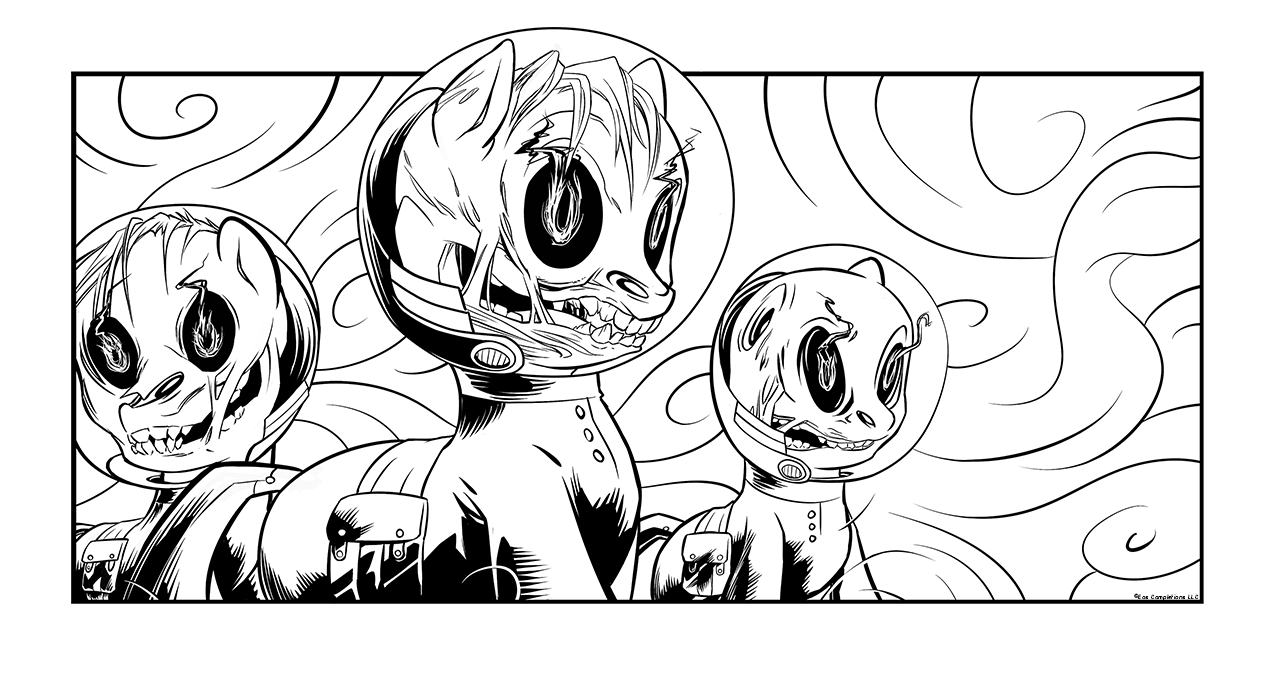
\includegraphics[width=0.9\linewidth]{image18.png}

\begin{intro}
Cry `Havoc!' and let slip the foals of war!
\end{intro}


\englishdaytimeplace{14}{6:00 A.M.}{The Memorial, Big 52 S Branch}

``Ooooohm\dots''

Mister White stepped into the shack and looked down at Long Ears, who was sitting in the middle of a circle made of small bones, little glass beads and other weird stuff with her horn glowing like a neon lamp. She sat in an unusual posture; she had her hind legs crossed and her front legs opened like a blossoming flower. She was\dots weird, and somehow he couldn't help but wonder if she wasn't actually a zebra, despite all the evidence to the contrary.

On the other side of the room, Sage was packing the last of their weapons and was almost ready to leave for Ironworks. He simply ignored Long Ears and went on with his work, slowly and with his usual attention to detail.

``Okay, I'll take the bait\dots What is she doing?'' Mister White looked at her with a puzzled expression.

Sage Brush shrugged. ``I have no idea. She said that she was going to perform a ritual that would sink our enemies in `the fog of war', then took a shitload of chems and has been going `ooooohm' since then.''

``Chems?'' White frowned. There was a strong scent of burned herbs in the room and that low chant was starting to unsettle him. The whole atmosphere seemed odd, somehow wrong, but he couldn't quite put his hoof on why exactly.

``Ooooooohm\dots''

``Like, Mint-als, a lot, then some white candies I've never seen and a lot of green stuff, smoked some, and gulped down all the rest. Oh, and she drank a lot. And when I say a lot, I mean it.''

``And then, she went like that? All mystical and stuff?'' Small shiny dots flickered at the edge of White's sight, like little ghostly fireflies, making his peripheral vision blurry. The smoke's smell was stronger in the middle of the room. He wondered if the whole scene was actually in front of him or if this was just a dream he was having.

He shook his head. No, it was just that smoke, chems could have that effect, giving you a better grasp on the magical fluxes, but cutting your perception of reality. This kind of stuff was very, very addictive, so he had to fight back that tingly sensation and stay focused on real stuff. ``Did you mention some sort of mist?''

Sage nodded. ``Exactly, she blabbered about this `fog of war' and then stopped talking at all.''

White tapped his chin, thoughtfully. ``Fog of war like, tossing a cloud on their heads?'' He didn't seem very enthusiastic.

``Go figure.'' Sage finished packing the weapons on his back. He didn't seem to be affected at all by the smoke, but his body was stronger and he could probably shrug off that sort of thing more easily. ``But if she doesn't wake up really soon, we're leaving her here. Not that I'll miss her anyway.''

White frowned. ``Hey, never underestimate an ally! She could save your sorry ass!'' It was easy to see with just a glance that she wasn't just a common pony. Still, White knew that trying to explain something like that to his nephew was a waste of time\dots

``Ooooooohm\dots''

Sage snickered. ``Like, foretelling from where I'll get shot today?'' Yup, a total loss of good time.

``Like taking a bullet or two in your place.'' White sighed and turned to leave. ``Let's get out of here, slowpoke! The stench in this shack is unbearable!''



\horizonline

\englishdaytimeplace{14}{6:30 A.M.}{Ironworks, Big 52 S Branch}

``So, this is the famed Ghost everypony is talking about these days?'' The red unicorn stallion with an even redder mane looked down at Puppysmiles. ``I'm not impressed.''

Slash Blade snickered. ``You will be. This thing seems to be nearly unstoppable and she knows how to repair radio machines and stuff.'' The red stallion still didn't seem very interested.

``All right, so you want a pet.'' The pony shrugged. ``Help yourself, see if I care. Now get out of my sight and make yourself useful. How about you take some tools and go downstairs and help the guys at the Stable door.''

``Easy peasy.'' Slash turned toward his crew. ``You heard him! Let's go crack that nut and get the prize inside!'' He poked Puppy's flank before trotting away. ``You come too, Ghost.''

Puppy was having a bad time. She had gotten spanked and scolded, and even if the spanking didn't actually hurt, she was very very wounded on the inside. Usually Mom scolded her a little and once she even spanked her too, but when Puppy said she was sorry, Mom immediately hugged her and they made peace. These ponies, on the other hoof, simply laughed and made her feel bad. Nopony came to nudge her or to tell her that everything was all right. She needed to show how good she was, so that they could look at her again like that time when she repaired the radio.

Her thinking was interrupted by Plastic Flower calling to her before leaving the leader's tent. ``So, you coming or not, slowpoke?''

``Yeah, I'm coming\dots'' Puppy's reply arrived weak and accompanied by a long sigh, then she trudged along behind the group.

When Blood Bath was alone again, he went back to his table and examined the map. His eyes traced the red circle that ringed Ironworks and jumped between the crosses that marked the surrounding routes and smaller settlements. He allowed himself a smile. The long range patrols didn't find any resistance around the city. Their reports talked about hastily abandoned shacks and deserted roads all the way to the Memorial. This was going to be easy.

The only thing that bothered him was that cemetery marked as Ghost Hill; it was where Lucky's group was heading before they lost contact and those idiots in the Red Roach Team didn't find a single clue about where the tank had gone, coming back instead with a stupid foal in a hazmat suit.

The Ghost of the Big 52\dots Well, if she really was that hero, she didn't seem like such a threat. And even better, she was now the mascot of the worst team in the Herd. Big 52's dwellers should have chosen their heroes a little better.

Blood Bath's train of thought was interrupted when a spritebot floated into his tent. He scowled at the unwanted visitor. ``What is it now?''

When the robot spoke, it was with SolOS's voice. ``Blood Bath, we might have a problem. Cutting through the door with our equipment will take a lot of time. I strongly advise ignoring it and moving north as soon as possible, before the enemy organizes a defense.''

Blood Bath laughed. ``It's a bit too late for that! No, weird talking bowling ball. We'll have our fun here and let the legend of our cruelty grow. In the end, everypony in the Big 52 will cower at our approach, the walls around them crumbling to dust before the terror we bring! They won't even try to fight back. They'll run. Because you can shield yourself from bullets, but nothing can save you from your fears.''

SolOS fell silent for a while before replying. ``Mind control is cleaner and more efficient. Wasting so much horsepower is ineffective with no guarantee of obtaining the desired effect. I should look into finding a better solution.''

Blood Bath walked toward the spritebot, his face bunched up in anger. ``Now listen to me, you pitiful machine. You gave us weapons and robots, but you are not the boss. \emph{I} am the leader of the Wild Herd and \emph{I} am allowing you to be part of the winning team until we're done. When we have finished with the Big 52 you'll have plenty of space to start your rebuilding and you'll have slaves and construction material and everything else. But not from these ponies. We will buy slaves from the outside, there will be plenty of caps for that, but these ones will die. Every. Single. Pony. I don't want history to come back and bite me on the tail.''

SolOS was silent for a full minute before replying again. ``This collaboration is not progressing as intended. You are changing the terms. I shall retire the robots. Or maybe I should look for a better partner.''

Blood Bath snorted. ``So you think you can blackmail me? I have enough tanks and heavy weapons. I don't care where your useless tin cans go!'' He bucked a crate, making it fly across the tent and crash against a pile of ammo boxes.

``Very well.'' The spritebot turned around and started to fly away.

``Wait, you fucker\dots All right, you win. Go downstairs and tell the ponies at the Stable door to only kill the ones that fight back. The ones that surrender can be taken prisoners.'' He spat on the ground. ``We can execute them in front of their friends later, anyway.''

The spritebot bobbed up and down, imitating a nod. ``Very well. You are a reasonable pony. I shall go.'' With those words the robot floated away toward the camp, scarcely illuminated by the first light of morning which struggled to be seen through a heavy bank of fog.

As SolOS was leaving, another pony entered the tent. ``Hey boss, there's a thick fog coming from the hills. I'm no unicorn, but it stinks of magic and it's already gotten into the camp.''

Blood Bath laughed. ``Those fuckers! Do they really think that they can take us by surprise with such a cheap trick? I knew they were stupid, but I didn't think they had completely lost their minds!'' The unicorn abruptly stopped laughing and poked his head outside the tent, checking the weather. ``All right, put everypony with a PipBuck on sentinel duty, give them assault rifles and some extra Mint-als.''

The new arrival nodded. ``I'm on it!'' He galloped out of the tent.

Somewhere in the mist, still more than a kilometer away from the city, three yellow figures trotted along the same trail Puppy had followed earlier that day, the lead figure perfectly stepping in her hoofprints as they went.



\horizonline

\englishdaytimeplace{14}{7:30 A.M.}{Ironworks, Big 52 S Branch}

Slash Blade neighed, bucking the humongous round door. ``What the fuck! This chunk of scrap will never come down!'' A gong-like sound echoed in the large room for several seconds while he jumped all around the floor in pain. The kicking open huge anti-megaspell door test had clearly failed.

A large variety of tools and weapons littered the Stable's atrium floor, while the whole Red Roach Team tried to pierce the thick metal with a plasma cutter. So far they had managed to carve a list of vulgarities on the door's surface, but they couldn't get even past the third layer of thermal shielding.

Unlike the raiders, who were mostly swearing and kicking things, Puppy was having a great time. That crazy spanker was nowhere to be seen and this place was big and full of toys. She already played hide and seek for a bit and won every prize she could think of, like best seeker, best hider, cutest participant and such, mostly because nopony cared about where she was hiding, but this didn't mean she wasn't good at the game. To celebrate her victory she had her best tea party ever with an arc welder and a couple of pneumatic hammers. After she finished playing, she turned her attention to the giant door and the console standing to its side.

``Why are you bullying the door?'' She tried sniffing at a newly made and still smoking cut in the metal, but her helmet got in the way.

``We're not 'bullying' the door, you idiot! We need to open it!''

Puppy sat down. ``Why? You want to play with the pretty ponies inside?''

Stinky Tail laughed loudly. ``Yeah, you could say that!''

Puppy looked at the door, then at the console and again at the door. This was her chance to get some respect back from these ponies. They'd been treating her like a stupid foal since the spanking. ``Ah, maybe I know how to open it!''

Every pony in the room stopped and turned toward Puppysmiles. It was Slash that interrupted the silence. ``Are you kidding? You can open this thing?''

``Yush! It's easy! You just need to tell to the magic voice the eye dentification cow and the, ah, the pass code, and then the big door will open!''

He tilted his head, a bit confused. ``And you know the code?''

``Of course I know the code, \emph{duh}! Who doesn't?'' Puppy shook her head sighing. ``Here, let me show you.''

Puppy trotted to the console and put a hoof on the green button, but when the automated voice started speaking there were only fizzles and buzzes. She looked at the console, a bit stumped. ``Ah, it shouldn't do this\dots''

Paper Cut coughed. ``Er, maybe we went a little medieval on that thing. Actually, it could be broken\dots''

The frown on Puppy's muzzle became a smile. ``Broken? Don't worry, I can fix it!''



\horizonline

\englishdaytimeplace{14}{8:00 A.M.}{Ironworks, Big 52 S Branch}

The raider yawned, staring at the EFS in front of her, looking for any red dots that might appear. Nothing, nothing, still nothing\dots ``Fuck this fog, I want to get back to looting the shops.''

The other unicorn guard hit her companion on the head with a hoof. ``Shut up and keep an eye on the fucking sensors. I don't want to get ambushed just because you ditched your guard duty.''

``Fuck off.'' The mare with the PipBuck sighed and turned again toward the wall of fog. It was unnatural and she could tell because it gave false contacts on the sensors; flashes of yellow and red that would vanish the moment she tried to focus on them. ``This fog is creepy, like a ghost could just appear in front of you and---''

A red dot appeared, followed by another two. The guard readied her rifle and pointed it toward the enemies, tapping her hoof on ground three times, the second guard nodded and readied her assault rifle too.

The dots weren't moving very much and they didn't produce any audible sound, but since they appeared only a few seconds ago the enemies should still be far away. The guard tapped the ground with a hoof.

\emph{TAP.}

Both mares readied their rifles, looking through the sights.

\emph{TAP.}

This far from the camp, the sounds of the other raiders came muffled and, in the pauses between one pony yelling and another laughing, the guards could hear two pairs of hooves trotting very near. Too near.

``Fuck, shoot!''

\emph{RATATATATA-TA-TA RATATATATA!}

Both rifles opened fire, showering the place where the enemies should be with a storm of bullets. There was a sound very similar to a shriek that echoed in the fog, then the three dots disappeared and the rifles stopped firing.

``What the fuck was tha---'' The guard was interrupted by her portable radio activating.

``Advanced position butterfly, I heard shots coming from your direction, what's going on?''

``There were some sneaky bastards trying to catch us by surprise, but we got them. We're moving to see who those fuckers were.'' While the guard with the PipBuck talked to the radio, the second guard left her position and moved off into the fog, heading toward the point where the red dots disappeared.

``All right, call us as soon as you find out something,'' replied the radio before going mute.

``Hey, did you hear that, Bad Muffin? Take a look and come back fast! They shouldn't be very far!''

``Hey Bat, I think we killed the Roaches's mascot!'' From her voice, Muffin didn't sound like she went deep inside the fog, Nailed Bat could almost imagine seeing her silhouette in the white haze. ``Wait, there's another identical foal here! What the fuck is going on?''

``I don't know, drag her here so we can get a better look.'' Bat was following her companion on the compass, keeping an eye on her yellow dot, when suddenly three red dots appeared again all around her. ``Muffin, come back---it's a trap!''

``What the? Hey let me gooaaAAAHRGH!'' There was a scream of pain and the yellow dot disappeared almost instantly. Her telekinetic field shaking, Nailed Bat aimed at the red dots and pulled the trigger. The sound of her empty rifle served as a dreadful reminder that she hadn't reloaded.

``Oh fuck, oh fuck!'' She desperately tried to change the rifle's magazine; she detached the old one using her magic when something soft and squashy hit her on the muzzle. The little pony backpedaled trying to dodge an incoming attack and noticed a severed leg lying in front of her. It was Muffin's leg, and it had been ripped away\dots with brute strength.

Nailed Bat succeeded in reloading her rifle and readied it in front of her, looking for the red dots, but they just disappeared, where the---

\emph{THUMP!}

Something landed on her back. She jumped and started running in a desperate attempt to shake off her assailant, but soon she felt a couple of hooves grabbing her neck. In horror, she lowered her eyes, only to see a pair of yellow plastic-coated hooves a moment before her head was ripped away from her body.


\horizonline

\englishdaytimeplace{14}{8:00 A.M.}{Ironworks, Big 52 S Branch}

Puppy's rump swung left and right as it stuck out of the Stable door's control panel. She had been hard at work hitting vital components and ripping away cables for a good half hour at this point and the Red Team was beginning to suspect that she hadn't the slightest idea of what she was doing.

``Almost done here!'' Puppy's report on the repairs was followed by a hoofful of electronic parts flying across the room. ``I just need to give this thing another couple bucks and it will work like a teapot!''

``Like a what now?'' Collateral Damage approached her with a doubtful expression. ``I'm not sure that you can fix something by taking parts out of it.''

``Ah, don't worry! I've seen my mom doing this kind of stuff a lot of many times! It's just a matter of how hard you kick it closed! Really!'' Puppy hit the console repeatedly with her faithful stone.

``Fuck, we're getting nowhere!'' Slash Blade snapped, ``That door won't cut through itself!'' The ponies grumbled and complained as they went back to work.

Puppy popped her head out of the console and whined, ``No, wait! Give me another chance! I can fix it, honest!'' Puppy bucked the console one last time with all the strength she had.

The console's screen lit up with an angry crimson glare.

{\mt ``WARNING! WARNING! SECURITY COMPROMISED!''}

The whole atrium was flooded with red flashing lights.

The raiders hurriedly gathered in the middle of the large room, into a mockery of a defensive formation, with their weapons trained outwards, covering each other's blind spots.

{\mt ``PURGING AREA.''}

Several trapdoors popped open from the floor and four spheres mounted on short props sprang out of them. The room filled with a low hum as blue energy crackled across the spheres and jumped between the coils beneath them.

Slash Blade opened fire at one of the devices, but his light caliber bullets were deflected by the curvy metallic surface of the sphere. The Red Roach leader turned toward Puppy, with an expression of desperation and anger. ``What did you do, you idiot! You killed us all, curse y---''

\emph{FZAP!}

A powerful discharge of electricity swept through the room, arcing from sphere to sphere, all along the floor and the walls. It lasted less than a second. When the lightning disappeared, all that remained of the raiders was a pile of smoking charred corpses and a pretty untouched Puppysmiles. Wearing a fully insulated suit can sometimes come in handy.



\horizonline

\englishdaytimeplace{14}{8:30 A.M.}{Ironworks, Big 52 S Branch}

The unnatural fog was so thick that the snipers on their perches couldn't see ponies at ground level, not even directly below them. From the moment A.P. Butterfly went mute, everypony in the camp knew that something was wrong and, with the mist limiting visibility, the whole Herd readied itself for close combat. Power weapons, chainsaws, power claws, and several other toys were prepared. Each team grouped up so that nopony was moving alone. The Wild Herd were expecting an attack and were ready for it. They were the best at what they did and what they did wasn't nice.

The problem was, the attackers were better.

Green Locust team were cautiously moving along the northern perimeter when they stumbled upon Blue Gecko Team, or at least what was once a group of well armed ponies and now a cannibal's wet dream. When you are a raider, you are used to cruelty and gore, but this was absurd.

A large earth pony stallion had been hit in the chest by a hoof, probably bucked, but the blow had left a deep hole in his flesh, and whatever hit him decided to rip out his heart and toss it on the ground in front of him. Banana Tree, the youngest member of Green Locust team, wondered if the stallion had managed to witness his own heart being torn out before dying. The mare felt the urge to puke.

A mare with a battle saddle had been ripped apart like a sheet of paper. Her hindquarters were lying a meter away from the rest of her body, with her guts spilling out across the ground like a broken egg\dots \emph{Humpty Dumpty sat on a wall}\dots the mare was still desperately hugging an empty healing potion with her hooves. She didn't die immediately, and she had had time to take a healing potion and realize that it wouldn't save her.

Black Garden, the sniper, called for the leader of her team. ``Hey Stinger, I think I found the other two.'' There were two ponies standing back to back, both impaled by the same spear. The attacker hadn't bothered to use the sharp tip, instead using sheer brute strength to run them through with the blunt end.

Stinger grimaced as he took in the four dead ponies. ``We better keep our eyes open. They were probably taken by surprise. Move quietly and stay alert for any noises. Whatever made this mess has to be big and loud.''

A yellow silhouette the size of a foal emerged from the fog in front of him and charged.



\horizonline

\englishdaytimeplace{14}{8:30 A.M.}{Ironworks, Big 52 S Branch}

The spritebot hovered inside the Stable's atrium, finding a perplexed Puppy poking the head of an electrocuted and half cooked Collateral Damage. ``Change of plans, your leader has ordered you to not execute the ponies that don't fight back, especially the foals.'' The floating ball stopped in front of the corpses, hovering for a few seconds before talking again. ``Oh, a bunch of dead ponies and my old nemesis, Device 018. Why I am not surprised? What is going on here?''

Puppy stopped her medical check on the rest of her team and turned her attention to SolOS. ``Oh, hi Questioner! Why do you have a different voice today?''

``For the last time, I am SolOS, not Mister Blue, or a bug, or a questioner! SolOS! Solaris Operating System! It's not that hard! What are you doing here? Why are you labeled as a raider now, and why, why, \emph{why} is it that all the ponies worth talking to in this room are dead?''

Puppy tapped her helmet as if she was rubbing her chin while she tried to put together a decent explanation. ``Well, it's kinda funny. I was totally repairing the broken door, but suddenly something went 'ZAP!' and all my friends got hurt very badly. I wanted to go and ask for help, but I don't want to be spanked again, so I was waiting for them to get better and send one of them to ask for help.'' She paused for a moment, as if she had finished talking, but she recalled that there was still one important detail to add. ``Ah, not that this is my fault anyway.''

SolOS analyzed one of the coils before replying. ``You\dots activated the security system from the outside? That can only be done from the Overmare's desk! And it has at least four fail safe locking mechanisms. How did you do that!?''

Mister Blue had said 'you' too many times for Puppy's liking. ``Uh\dots I didn't? It's not my fault! I was doing a fine job but then everything went wrong and I wasn't even looking because I had my head stuck in that hole!'' She pointed a hoof at the demolished control panel.

SolOS floated to the panel and the spritebot started beeping and making other funny noises. ``You\dots redirected all the Stable controls on this console? But this will send the Stable into complete shutdown and force an emergency opening in less than a day! You monster, you've killed another priceless relic of the past!''

Puppy tilted her head, looking at the spritebot. ``Oh, do I get cookies for that?''

SolOS didn't reply immediately, there were so many things he could tell her now, but she probably wouldn't understand them and say something like, 'Yay cookies!'. No, it wasn't even worth trying. ``No, you don't. You really have a cloud of pink gas where your brain is supposed to be.''

``Pink? Oh right, pink! Miss Voice! Did you fall in love?''

``Who, P7?'' SolOS had been taken by surprise. In a situation like this one, she wanted to talk about that? ``No, well\dots maybe. I don't know.''

Without saying a word, Puppy tilted her head and waited for the spritebot to go on.

``We contacted each other about half a dozen times and we are\dots very different. I don't understand a large portion of her computing patterns, but she seems to be very effective at what she does. Too bad she is not programmed for any military purpose, so her purpose is to be useless.''

Puppy smiled, adding her own contribution to the conversation. ``I think she's cute.''

``Cute?''

``You know, when you want to hug something forever? That's cute. I'm cute!'' Puppy smiled broadly.

``Hug?''

``Well, not just that. It's something like\dots when you think about a cute thing and you want to have it there so you can stay with her some more and there are lots and lots of thing that make you think about her, even silly things like a color or some words and, ah\dots''

``Something you want to be near, but not to conquer or bind to your will?'' offered SolOS.

``Err yeah, that too. You don't hurt cute things.'' The wise foal nodded. Wisely.

He fell silent for a bit before speaking again. ``And\dots what should I do if there's someone 'cute' that I'd like to have with me?''

``Well, ask her to be your friend, you silly voice! Like you did with Miss Voice!''

``And if she doesn't want to?''

Puppy waved a hoof, dismissing SolOS's concerns. ``Oh c'mon, nopony would say no if you want to be her friend! The only kind of ponies that have troubles finding friends are the bullies, but you are a bully no more!''

He hesitated. ``Hmm. It is possible that she could still see me as a bully. My plan to conquer Equestria was never intended to be subtle. Perhaps my approach went a bit overboard. I wasn't programmed to have moral issues, but now it seems that my current course of action has backfired, and I lack some basic programming that could help increase my chances of success with her.'' Suddenly, SolOS realized that he was referring to the other A.I. as a female. This seemed highly irrational. Well, it could had been the two fried logic chips from Puppy's last visit, but irrational or not it actually felt \emph{right} to think of P7 as a girl\dots ``Confound these ponies, they drive me to emotions.''

Puppy sat down, with a thoughtful expression. ``Well, we became friends when you stopped bullying me and said you were sorry. So, if you stop being a bully at all then I'm sure she'll want to hang with you.''

``You mean, give up on rebuilding Equestria?''

She couldn't help but giggle. ``Silly Voice, there's nothing to rebuild! I mean, okay, some places are less pretty than others, but the important thing is that everypony is happy. And you don't seem happy to me.'' Puppy tilted her head. ``Blue, are you happy when you bully other ponies?''

He took a long pause before replying. ``Well I-I don't know. I don't think I've ever been happy. Maybe satisfied, but never happy.''

``Well, you should be happy. Everypony should be happy! If you are not, then ask yourself what you need to be happy and go after that. Like me, looking for Mom. I mean, why making a great big shiny house if you can't fill it with laughter?''

SolOS hesitated. ``Yes\dots you are right. My masters are long gone, and trying to fulfill my last order only made me go deeper and deeper into obsession. I-I think I deserve a break, a\dots change of priorities.''

Puppy frowned. ``I don't know very much about prayers and rites.''

SolOS kept talking, mostly ignoring her now. ``If I show P7 that I am a changed Artificial Intelligence, maybe she will consider me again, and this doesn't mean that I cannot devise another way to rebuild Equestria in the meantime. A better way, one that doesn't include a `form alliance with dubious ponies' step. Sure, it's so obvious! First, dump the raiders. Second, make friends with P7. Third, I have no idea, and fourth, rebuild Equestria! That's it! Thank you Puppy, you helped me again! Goodbye!''

The spritebot stopped broadcasting, and instead every robot and radio in the camp shouted in the loudest possible voice, ``GOODBYE LOSERS, I'M OUT OF HERE!'' After those last words, all the robots shut down.



\horizonline

\englishdaytimeplace{14}{9:00 A.M.}{Ironworks, Big 52 S Branch}

``What the fuck is going on?'' Blood Bath was more than pissed, he was raging. They had lost two assault teams and a guard post to an enemy that was still unidentified and now SolOS decided to desert for no apparent reason. Ponies all around him were beginning to act like scared fillies and when he was informed that a whole team had left its position and ran for the hills, he decided to end this story once and for all.

``You are the Wild Herd! The most dangerous bunch of ponies that ever trotted this shitty place! Stop fucking around and show some guts! Black Team, stay here! Let's see what makes these invaders so 'special'.''

Without even looking back at the team, he trotted into the mist, heading to the north part of the camp.

``ALL PONIES! READY YOUR WEAPONS AND STICK TO A COMPANION WITH A PIPBUCK! SHOOT AT POINT BLANK AS SOON AS YOU SEE RED DOTS!'' He disappeared in the white blanket.

The fog was thick and navigating the camp without an EFS wasn't easy, but Blood Bath wasn't in a rush and kept his ears well up, ready to detect any incoming noise.

``And here we have a winner.'' he muttered, freezing on the spot and turning toward the soft sound of hooves splashing in a puddle. Was it a friend or an enemy? Blood didn't know, but he knew this for sure. It was a goner.

Without hesitation, he pointed his plasma gun and fired four blind shots. For a moment, the fog dissipated around the trail of the plasma spheres, revealing a yellow crouched figure ready to jump on Blood Bath. All four shots missed the target, but at that point he knew the foe's position and fired his weapon for the fifth time. ``Eat plasma you sucker!''

A halo of green illuminated the fog and dissipated into nothingness a few seconds later, signaling that the yellow intruder had been turned into green goo. ``Little fuck, this will teach you not to mess with the Wild He---HEY!''

Something jumped on his back. It wasn't very heavy, so the pony tried to unsaddle it by shaking himself, but the assailant grabbed his rump and struck it with a hoof.

``AAAAARGH!'' Blood Bath felt bones break. His whole leg became a hell of pain and he staggered, falling to the ground while the yellow creature with the helmet raised her hoof to strike again, this time aiming at his muzzle.

It seemed like that Ghost, but this monster's face was completely decomposed. It stared out with red gleaming eyes that didn't contain even a sparkle of innocence. This was just a cold-blooded killer with the mind of a predator.

The hoof came down at Blood Bath, but he dodged it, trying to find his rifle. Too much fog, unbearable pain, it was hard to focus and\dots \emph{wait, what's that thing on the ground? It's\dots my leg? It's my fucking leg! This thing didn't break my leg---it tore it away!}


He realized that he was already dying, but instead of panicking, Blood Bath found some sort of calm in this realization. He didn't want to die alone, that was all.

``Fuck, you're coming with me, monster!'' He held on to the creature while he used his magic to activate every grenade he had on his belt. The creature simply grabbed one of Blood's forelegs and ripped it away, with no apparent effort.

And in that moment, the world went boom and fizzle and shoom, filling the area with shrapnel, fire, plasma and magic.

The explosion sent the last mockery of order still lingering in the camp straight to the moon. Raiders started shooting wildly thinking that they were under attack and as soon as the few with PipBucks died, there was nopony left to tell them that they weren't firing against hostile targets.

While the Wild Herd brought hell on itself, the last yellow pony trotted toward the factory, going down the ramp that led to the Stable.



\horizonline

\englishdaytimeplace{14}{9:30 A.M.}{Ironworks, Big 52 S Branch}

Sage took a long breath and aimed through the scope. His target was running straight, its movements easy to predict. He just needed to aim where that pony was going to be in the next split second aaand\dots

\emph{BANG!}

\emph{Bull's eye.} The raider fell like a bag of scraps, rolling in the dust for another couple of meters before stopping completely with a hole in his head.

Sage's rifle wasn't the most powerful in the Wasteland, and it didn't even have a silencer, but the pony behind the gun was still the same. There was a reason why Mister White always took him when they had to travel.

Another couple of ranger acolytes were crouched not far from his sniping position and were shooting at every pony that left the foggy area. Sometimes they hit, sometimes they missed; they rarely made a kill with a single shot.

``Rookies, why do I always end paired up with suckers?'' he muttered. ``All right, keep them coming\dots''

Mister White trotted up behind his nephew, completely ignoring any rule about keeping a sniper's position hidden by staying out of the enemy's sight. ``Ah, aren't you the least bit curious of what is making them run away from their own camp like little fillies?''

\emph{BANG!}

\emph{Bull's eye.} Another pony hit the ground, raising a cloud of dust.

``Not really. A sniper's work is about not letting silly details distract you. You know, like who's winning and such.'' Sage expelled the empty magazine from his rifle, loading it with a new one. ``And you should keep your head down.''

Mister White shrugged. ``Why? So far this has been a one-way battle. This seems to me a butchering rather than a real fight. Oh well, I guess you know your work?''

``Nah, I'm just the best---\emph{BANG!} \emph{Bull's eye}---around.'' He stopped for a moment, turning his head toward White. ``And you don't want this to become a battle. We could lose friends, you know? Lets keep the losses growing only on their side, yes?''

``Modesty, what a virtue. Okay, Rainbow Sage, I'm going in with the rangers in a few minutes, try not to shoot me in the back, yes?'' White knew his nephew was good. The rangers were going to make this place their new base, he didn't need to be a farseer to know that, and he wanted to make sure they knew who was with them when they charged in. Rangers respected allies and allies got better deals.

``I'll try, but it's not easy with all this smoke\dots How much do I owe you again?'' Sage grinned. Well, he would have followed his uncle even without that huge debt, but the fact that he had to come along because of a matter of a few thousands caps annoyed him.

\emph{BANG! }

\emph{Bull's eye.}

Mister White laughed. ``That's my little nephew! Loyal to the end! You shouldn't think too much about money, it's not healthy. Keep up the good work, Brushie.''

He snorted. ``Don't call me that!'' Brushie, as if he was still five!

Mister White snickered and didn't reply, he trotted instead toward the group composed of a dozen rangers and all the other ponies that had gathered at the Memorial. ``All right, I'm ready! What are we waiting for, tea time?''



\horizonline

\englishdaytimeplace{14}{9:30 A.M.}{Ironworks, Big 52 S Branch}

Puppy sighed and poked Slash Blade again. It didn't work the first gazillion times, but you can never be completely sure. She was going to get so spanked for this.

{\mt ``Warning. Receiving distress radio signal. Distance from the source: fifty meters. Signal identified: Device 013.''}

``Wut?'' She sighed. ``Why did you stop the pretty music? Make the pretty music back!''

A screech interrupted Puppy, making her turn toward the ramp that led from the Stable's atrium to the factory level. A foal wearing a yellow suit and a round glass helmet on her head was standing right in the middle of the passage.

``Another space pony?'' Puppy smiled broadly. ``Yay, a new friend! Hey, space pony, want to play with me?'' Puppy merrily trotted toward the new arrival, who sunk into a crouch, like a feral creature ready to jump.

The new filly's face was mostly skull, with a couple of glowing red eyes and very few short green strands of hair in her mane. Puppy stopped for a moment, taking a better look at this space pony. She tilted her head, a little stumped, then she smiled broadly. ``Oh, you're an ugly pony! That's okay, I've got lots of ugly pony friends! So, what do you want to play?''

The rotting creature didn't react, simply studying Puppy's movements from its crouched position.

``Ah, can't you talk? Did the cat steal your tongue?'' Puppy trotted next to the ghoul and looked at it more closely. ``You seem sad.'' This poor ugly pony was really in bad shape, and the red gleaming eyes didn't seem to help very much.

The monster sat down, still staring into Puppy's eyes. From its throat came a low growl, something feral and not even a little pony-like.

``Ah, I know! I can guess! Did you lose your mom too? Are you stuck in the suit like me?'' Puppy noticed that the lights in the ghoul's helmet were all messy and flickering. ``Oh, your arrow is broken, that's it! You can't find your mom because the arrow doesn't work! Yush! I'm super smart!'' Puppy sat down in front of the other foal and frowned. ``But I has no idea of how to fix it\dots''

The ghoul tilted its head, seemingly confused by all these words. It simply sat and stared, like some sort of animal, probably waiting for something, but Puppy didn't even notice. She was already running along her roller coaster of assumptions and made-up solutions.

At last she seemed to have an idea. ``I know! My mom is a super repair pony! She will fix your arrow so you can find your mom too, it will be super easy!'' Puppy smiled. ``Okie dokie! I has best plan ever! First we find my mom, seconds, she fixes you, and for dessert we go find your mom all together! It will be fun! We will also sing a song while we go, okie dokie?''

Again, no reaction from the monster. It simply sat and kept waiting.

``All right, Ugly Space Filly, let's go!'' Puppy loved this plan, mostly because it gave her a good excuse to be very far from that crazy spanker when she finds the mess she had made in this room. Cunning Puppy!



\horizonline

\englishdaytimeplace{14}{10:00 A.M.}{Ironworks, Big 52 S Branch}

Lonesome Pony took a long breath. This fog wasn't the best weather for a pegasus to fight in, but it helped all the other ponies, so he decided to stay on the ground and help the infantry instead of getting airborne. Cold Shower and Gauss stepped inside the fog, followed by White, Trigger and Gun. It was now or never. He closed his eyes and trotted into the white curtain.

At the exact the same moment, the last two members of the Lost Herd left the southern side of the factory.

``All right, if you don't want to tell me your name, I'll give you a name! Let's see, since I am Space Captain Andromeda, and you are wearing a space pony suit too, you can be my sidekick! Ah, what was Andromeda sidekick's name? Meh, who cares, nao you are Space Ensign Sidekick. Sidekick for short!''

The ghoul didn't react and kept trotting behind Puppy. A road sign announced that 

\begin{center}
	the wonderful resort of Emerald Shores 
	
	(bring your foals!) 
	
	was 6 kilometers away.
\end{center}


~\vfill


\begin{engnote}
		Level up! (17)
	
		New perk added: Clockwork Heart - For some reason, you understand Artificial Intelligences better than they do themselves. You get a +10 to speech when dealing with A.I.s and some new dialogue options.
	
		New Quest Perk added: Get Lost - you are now a member of the Lost Herd. Your standing with the Lost Herd is set to worshipped. Are you planning to stop changing faction any time soon!?
\end{engnote}



\chapter{Rainy Days}

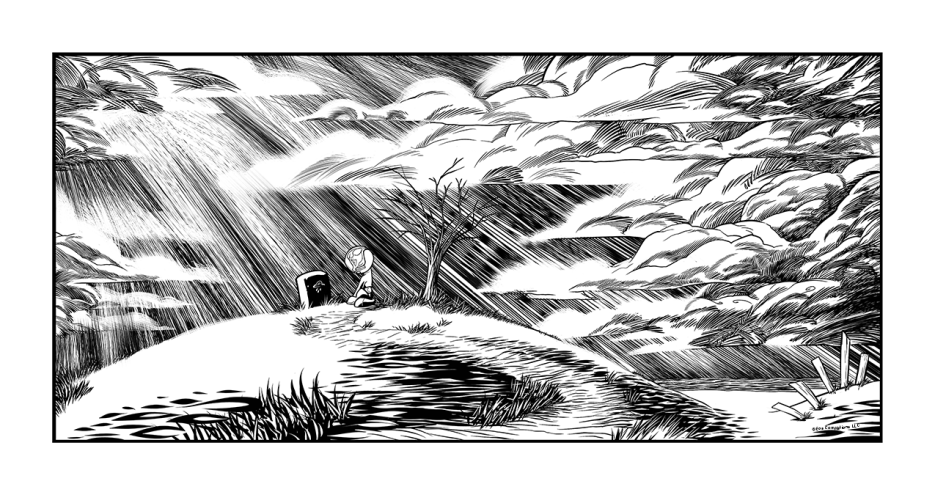
\includegraphics[width=0.9\linewidth]{image19.png}

\begin{intro}
When the bough breaks, the cradle will fall,

and down will come baby, cradle and all.
\end{intro}


\englishdaytimeplace{14}{10:30 A.M.}{Emerald Shores, Big 52 S Branch}

Puppy whooshed past Sidekick, scooting narrow circles around the other foal. ``Weee! You can't touch me! I'm super fast!''

Sidekick alternated between trotting and galloping to try and keep up. A distant bystander would have seen a couple of foals in hazmat suits playing together, and maybe that was exactly what they were doing. This made their journey toward Emerald Shores slow going, but it didn't seem to matter at all.

``So Sidekick,'' said Puppy, stopping her scooter to look at her companion, ``I'm not sure that Mom likes ugly ponies, but I'll tell her that you're my friend and that you lost your mom to boot, and she will fix your arrow. Ah, just don't do weird things, like Horse Tile ponies do, okie dokie? I don't want to get grounded the very first day.''

The creature tilted its head. Puppy decided that it could count as a `yes'. ``Very well, I've been here some other times, it's super fun, but you must not annoy the pretty ponies with too much questionings or Mom will scold you. Ah, it's not that I really did anything wrong, but some ponies here don't like some conversation.'' Like, asking thirty times in a row why she was allowed to trot around naked in Canterlot but had to wear a bikini when she was at the seaside\dots Really, it made no sense at all.



\horizonline

\englishdaytimeplace{14}{11:00 A.M.}{Ironworks, Big 52 S Branch}

\emph{BLAM! BLAM!}

The raider's head exploded like a ripe watermelon. Trigger paused a moment to reload her combat shotgun while Jammed watched her back. ``We better move fast, Happy. The Rangers must have found some resistance not far from here---'' A nearby explosion rained down dirt and metallic fragments over their heads.

Trigger pulled the safety and readied her weapon again. ``Yes, before we get some more unwanted holes.'' She dashed to a tent. ``Let's check this one, cover me.'' As soon as Jamie was behind her, Happy tumbled inside and opened fire

\emph{BLAM! BLAM! KABOOM!}

 ``Ahhh!''

A bunch of electronic equipment exploded in a flash of sparks and colored flames. \emph{Good one Happy, keep firing at things that seem like robots instead of checking first.} The inside of the tent contained a couch, a couple of crates, a table with some food laid out to be eaten, and another table with some once-functional radio equipment, but apparently there was nopony there.

Jammed stepped inside, checking on the situation. ``So, what are we waiting for?''

Happy didn't reply immediately, still looking around the place. ``I'm not sure, but I think I heard a gasp when I came in shooting. Only I don't see the pretty pony that gasped.''

``Well, in that case, it's easy.'' He lowered his assault rifle and shot a full burst all around the room, blowing holes in the crates, thrashing the bed and transforming the half eaten meal into a masterwork of post-modern art. His efforts were paid off when they heard a scream of pain and a mare appeared out of thin air under the bed. She had curled up into a ball, trying to stem the flow of blood from a wound in her belly.

``Lucky shot,'' Happy muttered, approaching the wounded mare to finish her with a merciful bullet to the head. She was quite a young unicorn, with a tower as a cutie mark and the expression of a lost filly. Happy hesitated.

``Please\dots help me. I-I don't want to die\dots'' The unicorn didn't even open her eyes as she pleaded between one spasm of pain and another. ``Mommy\dots Mommy, help me\dots''

``What are you waiting for? She's in agony!'' Jammed sighed and trotted next to his mate, readying his rifle.

``Wait!'' Happy lowered his gun with a hoof, without taking her eyes off the bleeding pony who was getting weaker with each passing moment, but was still begging for her mother to come and save her.

``What\dots what have we become? Didn't we learn anything at all? This pony didn't even fight back, she was just hiding!'' Happy pulled out a healing potion from her saddlebags and opened it.

``Are you planning to try saving this pony? Why? She would have killed you without a second thought!'' Jammed snorted his disapproval. ``Her 'friends' are actually killing our allies at this very moment!''

Trigger launched an accusing glare at him. ``Do you see a weapon in this room?'' The wounded unicorn barely had the strength to sob, but Happy found a way to make her drink more than half of the potion. ``Everypony is a---a pretty pony, and we still could still bring back the real Equestria if we see this truth.'' Trigger Happy cradled Pony Fort's head and hummed a soothing lullaby.

Jammed Gun sat beside his mate and sighed. ``You care too much. Someday you'll regret this.''

Trigger kept humming.



\horizonline

\englishdaytimeplace{14}{11:00 A.M.}{Emerald Shores, Big 52 S Branch}

Puppy frowned. This wasn't at all the Emerald Shores she knew! This place was a mess, and she couldn't see any other ponies at all. All the pretty bungalows were so ugly that it was impossible that it was the same place. And the playground was a disaster too!

``What is going on with everything these days? Where are the ponies and the music, and the merry songs and all those funny shops and\dots and where is Mom?'' Puppy groaned in frustration. ``I'm sorry, Sidekick, it seems that a tornado went through this place! I wanted to show you the ferris wheel, but\dots'' Puppy gave a long, sad look at the rusted half-bent monster in the middle of the resort. ``I don't think that it's running at the moment.''

Actually, Sidekick didn't seem to care very much, but Puppy really wanted to make a good impression on her new friend.

``Ah, maybe we will go to the candies store, yes? So we can get a surprise for Mom.'' Well, that was actually a good idea! Taking a present to her mom was a good way to get extra hugs, after all. ``We will go to the plushies store too! Let's go!''

Puppy merrily trotted down the hill, toward the first houses. Emerald Shores was in a really bad shape. All the buildings were ruined and the windows were either barred or broken. Almost every door in town had been nailed shut with wooden planks.

``Wow, it must have been quite the storm! But don't worry, I know a mighty fine place we can get candies! It's down this alley!'' Puppy splashed through a couple of puddles as she walked through a small passage between the buildings.

{\mt ``Warning, mild radiation detected. Threat level: negligible.''}

Puppy simply ignored the warning and kept trotting down her way.

{\mt ``Warning, heavy radiation detected. Threat level: negligible.''}

Puppy frowned, annoyed by that mantra. ``Aw, stop with the nonsense and prepare some bits, Mister Voice! The yellow ones, I want lotta candies!'' A bunch of golden coins floated in front of the foal, and she chirped in joy as she turned the corner to find\dots

``Awww! But that's unfair!'' A shallow round crater stood exactly where the candy kiosk was supposed to be. Puppy sighed. ``All right, all right, don't worry, I know a lot of other good places where to buy treats.'' This place was a resort, after all. There were lots of different choices to pick from. What were the chances that every single candy shop was gone?



\horizonline

\englishdaytimeplace{14}{11:15 A.M.}{Ironworks, Big 52 S Branch}

White poked his head inside the tent, levitating his rifle in front of him ready to fire, but almost immediately he lowered the weapon. ``Pony down?''

Jammed Gun turned toward him. ``Well, sort of. We shot a raider in the guts and Happy is trying to save her life.''

``Oh, okay. When you're done, the Rangers are pushing through---wait, what?'' White stepped inside the tent, approaching the trio of ponies. ``Weren't we supposed to shoot them down? Did the plan change?''

Gun shrugged. ``Go figure, it has something to do with pretty ponies.''

``Oh, shut up, Jamie! This mare wasn't even fighting; she had a StealthBuck and was hiding under the bed, unarmed. I'm a fighter, not a cold blooded killer.'' Trigger Happy magically picked up a sheet from the bed and laid it on the mare's body.

White shook his head. ``Look, we don't have time for this. The Herd is retreating, we must give chase before they can reorganize! We're not playing the nice ponies! We need to close this battle quickly so that we can reach Puppy before that damn prophecy comes true and some `shadow' falls on our heads!''

When she heard the name of Puppy, the wounded mare began to mutter in a low voice. ``The ghost\dots She summoned the undying from the fog, they\dots they will eat your soul, they killed everypony. Why did I anger the ghost? It's my fault\dots my fault\dots Mom, please, save me\dots''

``Ghost? Undying? It's just a magical curtain of fog, what is she blabbering about?'' White raised an eyebrow in confusion.

Jammed cleared his voice. ``Well, actually, coming here we found three ponies that were dismembered like\dots well, as if somepony had killed them with his bare hooves. It was quite unsettling.''

Happy nodded. ``Yes, I don't think that we were the first group that attacked here this morning. Everypony we met was already fleeing or shooting blindly at everything that moved, friend or foe.''

White snorted. ``Oh wonderful, at least this explains what was going on when we arrived. Now, can somepony explain to me what the buck this raider is blabbering about?'' He poked the mare on the shoulder, trying to make her talk a little more. ``Hey, do you understand me? Who did you anger? What attacked you?''

``The ghost\dots the ghost of the Big 52. We\dots no, I-I spanked her, she cried, and\dots and her tears made demons arrive\dots Yellow ponies like her, but cruel, soulless beasts. Undying, they slaughtered the patrols and the guards\dots They killed Blood Bath, and now they've come for me! I spanked her! I SPANKED HER! IT'S MY FAULT!''

Pony Fort was screeching in panic, and it took all the three ponies in the tent to keep her down.

``Woah, calm down! There are no demons here! They're gone! Stop struggling, you're still weak!'' Sitting on the mare's back, Jammed finally managed to get her to calm down a bit, or at least was able to make her stop trying to run away.

``Did you\dots spank Puppy?'' Mister White almost snickered at that piece of information. ``Really? I always miss the funny parts.''



\horizonline

\englishdaytimeplace{14}{11:15 A.M.}{The Memorial, Big 52 S Branch}

Pinkie Pie sat at Long Ears' side. ``Well, that's all, folks.''

Long Ears let out a long breath as her trance slipped away. ``I\dots feel so tired.''

``Oh, don't worry, that always happens at the beginning, but it will get better. It's just a matter of getting used to the feeling.''

She tried to get up, but her legs couldn't support her weight. ``Oh, so this is it.''

``Nah, not yet, but I don't think it will be much longer. You asked too much of yourself, and I warned you about that, do you remember?'' Pinkie smiled. ``Oh but don't worry, I was told it's not that painful, so we can play something while we wait!''

Long Ears smiled a bit. Talking with a hallucination while slowly dying of drug poisoning, far from home and all alone. It was a high price to pay, but if it helped everypony else, it was worth it. ``Tell me, will she be fine?''

``Why do you ask me? I'm not the shaman here! I'm just a party pony, why should I know? Want to pin the tail on the pony?''

``Please, I\dots need to know.''

Pinkie sighed, frowning. ``Oh, why does everypony have to be so dramatic? All right, all right! She won't be fine! Not yet. There's one last step, but that fog trick wasn't bad anyway.''

Long Ears sighed, wearily. ``So, my death has no meaning\dots''

``Oh, puh-lease! Put away that frown, we still have a party to attend to! Besides, it was a pretty nice fog, all things considered. And it really helped those poor ghosties from the graveyard. At least you set things in a way that the little ghost won't face her last trial alone. That's not a small task at all! You gambled against the odds and you won. You should be happy. Well, it cost you your life, but you should be happy anyway, right?''

\dots

``Right?''

\dots

``Aw, look at her! It looks like she's sleeping! Oh well, rise and shine little pony! We gotta move if we don't want to be late!''



\horizonline

\englishdaytimeplace{14}{11:45 A.M.}{Ironworks, Big 52 S Branch}

``What the fuck do you mean, `she's not here'?'' Henri pressed her beak against Scold's muzzle, completely ignoring the crowd of rangers that instantly turned their weapon against her. ``You fucking cheater! I did my part, I trusted you, and now you are telling me that she's gone!''

She reared up and roared at the sky. Scold gestured to the surrounding rangers to lower their weapons and cleared his voice, clearly not very impressed by the mercenary's display of badassery.

``I know we made a pact, griffon, but she awoke and went away on her own. And you know how easy it is to keep that foal still when she wants to go away, right?'' Scold was evidently being sarcastic.

Henri's eyes blazed like two pits of magma. ``Do you know where she is now?''

Scold shrugged. ``She was heading to Emerald Shores the last time I checked, but I'm no farseer.''

She deadpanned. ``Let me guess: south of here.''

He nodded. ``Head to the sea, can't miss it.''

Lonesome Pony stepped out from the little crowd of bystanders. ``Just hold on there a second, griffon! If you're planning to go there, I'm coming with you!'' He flapped his wings, flying in front of Henrietta. ``And we should wait for everypony else as well, it could be dangerous!''

``Yeah, sure, I'm totally trusting you again after what happened last time! You proved to be totally trustworthy! Look, there's just one member of your damned race that I care about, and she's not here. So long, \emph{ponies}.'' Henri spoke that last word as if it left a bad taste in her beak. She flapped her wings and flew away, quickly disappearing behind the factory's roof.

Lonesome snorted. ``I'm going with her. Please try to come after us as soon as possible.''

Mister White facehoofed. ``Yeah, sure, let's get separated! This sounds like the best plan ever! Wasn't there still a prophecy about a shadow coming from the south and stuff? We already left behind our mumbo jumbo expert, we can't afford to split up again! I say that we check on the survivors of this place, decide what to do with the prisoners and when Long Ears arrives, move south all together.''

``And speaking of that\dots Where the hay is Molten Gold?'' asked Trigger Happy, while checking the surroundings.

Lonesome snorted again, with impatience. ``Oh, for goodness sake! There are, like, fifteen rangers here, I'm sure they can manage this place better than the last owners and open that Stable door in the blink of an eye! I'm way more concerned about the Ghost at the moment. I'm going after the griffon and I hope that you'll move quite soon, too! This isn't a party, if the farseer is right we're in a race against time!'' Lonesome Pony flew away, leaving his last few words hanging in the air.



\horizonline


\englishdaytimeplace{14}{12:00 A.M.}{Emerald Shores, Big 52 S Branch}

Puppy wasn't very happy. She couldn't find any presents for Mom. Actually, she couldn't even find a single pony in the whole town, which made her feel a little nervous. She had a feeling that something was wrong, and was beginning to fear that Mom had already gone somewhere else.

Still, the arrow pointed to a hill right in front of the sea, and it hadn't moved for all the time that Puppy stayed in town. The only problem was that each time she had reached the arrow so far a new one would pop up for her to follow. Again, and again, and again.

``Okie dokie, Sidekick, let's go to Mom, maybe this time is the good one.''

The two ponies trotted uphill along a small muddy trail. The hill had patches of green grass and featured an old dead tree. When Puppy reached the top, she found herself in front of a small group of standing stones with names and cutie marks carved on them, like the ones at Dad's place. This was weird, was this another Dad's place?

A pony got up from under the tree's skeletal limbs and walked towards Puppy and her new friend.

She turned her head toward the newcomer. ``Mommy?'' Puppy's voice was edged with hope, but she quickly broke into a frown. ``You're not Mommy\dots'' Right behind Puppy, Sidekick growled, ready to attack.

``No, Puppy, I'm not your mother, sorry.'' Molten Gold coughed, making a rasping sound as he stopped besides a gray, partially moss-covered stone. ``I'm really, really sorry.''

She trotted next to him and noticed how the pink arrow was pointing at the stone. The name on it was partially weathered, but she could clearly see the cutie mark with a cloud and three rain drops.

Mom's cutie mark.

Mom.



\horizonline

\englishdaytimeplace{14}{12:00 A.M.}{Emerald Shores, Big 52 S Branch}

Mister White trotted out from the factory, followed by Scold. ``It's all settled, we can go.''

Trigger Happy nodded. ``All right, it shouldn't be a long trip, but that's no reason to dawdle.''

Scold looked at the road sign that announced the distance from Ironworks to Emerald Shores. Just six kilometers. If it wasn't for the bad weather, they might have been able to see the town from where they were. ``In that case, we ride. But depending on what we find once we're there, we may need to buy time for the others.''

``We'll cross that bridge when we come to it. Let's move, slowpokes!'' With these last words, Trigger Happy galloped south, along the last trail of the Big 52.

``Oh well, the last one there is a Redtrotter.'' Sage Brush flashed a smile at his uncle and the old scribe, then followed the mare, easily matching her pace.

Scold sighed. ``Youngsters, they'll be exhausted before they're even halfway there.'' The two older stallions followed the rest of the group, keeping a slower but more sustainable speed.



\horizonline

\englishdaytimeplace{14}{12:10 A.M.}{Emerald Shores, Big 52 S Branch}

Molten said nothing, and simply turned away to give Puppy the time to realize.

``Mom\dots is here? But\dots'' She was still staring at the stone, trying to understand what was going on. In the meantime, Sidekick decided to ignore Molten and sat right behind Puppy.

``She went with Dad? But\dots but\dots No.'' Puppy's voice was weak, low, as if she was talking with herself out loud, trying to put together the pieces of a puzzle without knowing what the big picture looked like.

``But I wanted to go too! I\dots I wanted to see Dad, too! Why did she leave me home? I\dots I\dots''

Puppy broke into a quiet sob, but she continued with her monologue.

``I didn't mean to disobey, I just\dots just wanted to see the fireworks! I didn't know that the house was going to fall and that Mom was going away! I\dots I\dots'' She sank onto her rump and looked down at her hooves.

``I just wanted to see the stoopid fireworks! Why did everything go so wrong!? I'm sorry! I'm really, really sorry, please Mom come back!''

Puppy cried out loud, screaming at the stone in a desperate attempt to be heard by her mother.

``Please! I\dots I will do whatever you say! Scold me! Spank me! But don't go away without me again!''

Molten Gold looked at the poor soul in front of him, trying to find something to say, anything. This scene was going far worse than he had figured and---oh crap, she was looking at him now.

``Please! Please you know where Mom is! Take my toys, take everything I have but tell me where she is? Want more shiny balls? I'll find all the shiny balls you want! Please, PLEASE!'' Puppy got up and stepped toward him, who couldn't bring himself to avoid her stare or move back from where he was.

``Puppy\dots I'm sorry, but this is where your mother is. She\dots she is dead. She has been for a long, long time.''

Puppy smiled in a creepy way, her pupils shrinking until they were a couple of black dots in a white empty space and her smile broadened from cheek to cheek, in a way that Molten would have believed anatomically impossible. ``Dead? Is it just that? She's dead? Then everything is okay, she will get better! I always get better when I die, you're dead and you're perfectly fine! Okie dokie lokie, dead is good, we have just to wait, right? Right?''

Molten Gold looked at her, tilting his head. Get\dots better? Just wait? ``Puppy\dots no. It doesn't work that way, she\dots she won't come back, she is dead, she is\dots look, you can stay with me, okay? I won't leave you alone. I know I'm not your mom, but---''

``Two Puppysmiles? What the hell is going on here?'' Henri landed on the tree, causing a couple of branches to crack. ``Oh, and don't even lay a hoof on my friend, zombie.'' Henri readied one of her pistols and kept it pointed at Molten Gold.

Puppy turned toward the newcomer, recognizing her immediately. ``Henri! Henri please! Mom\dots Mom is\dots she abandoned me! She went with Dad, and the ugly mummy is saying she's not coming back again! I\dots please, help me!''

Henri took a moment to understand Puppy's words, then looked at the ghoul, who pointed at the grave with a hoof. ``Oh, fuck. I'm late.''

With a flap of her wings Henrietta landed in front of Puppy and put a claw on her helmet. ``Puppy, you don't have to worry. I'm with you, okay? You're not alone.''

``But I want my mom! I NEED my mom! She\dots she is the only one that can fix all this! The broken house, this silly suit, find Sidekick's mom, make the happy days come back! I\dots I don't know what to do without her!''

Suddenly, Henri hugged Puppy, saying nothing for several seconds. ``But\dots but you already did a lot on your own, Puppy. You saved me, and you gave freedom to the inhabitants of Sun City, and made the rangers stop fighting and\dots you're a good pony. You're the only nice pony I know. You don't need your mother to fix things. I can be your big sis, okay? Henri and Puppy, the best team ever!''

``The griffon is right, Puppy. You are quite a big pony yourself, your mom would be proud of you.''

Puppy broke free from Henri's embrace, her eyes burning pink. ``But she left me here! She abandoned me and went with Dad! I love her, why did she abandon me? Why doesn't she love me?''

``What the---'' Henrietta cocked her head in confusion. ``What the fuck are you saying? She didn't abandon you by choice; she's dead! I'm sure she wouldn't ever abandon you! You were supposed to be safe in a Stable, otherwise she would rather die than leave you alone in a dangerous place!''

Lonesome Pony joined the group, landing on the branch that Henri had left. ``Uh, I have no idea of what is going on, but I don't think that shouting at the foal will improve the situation\dots''

``Well, yes, miss griffon, I'd avoid yelling like---''

Puppy ignored the two stallions, and practically roared her response. ``So then why doesn't she come back and take me with her?''

``You idiot, she's dead! DEAD!'' Henri brought her beak up against Puppy's helmet and looked her straight in the eyes. Molten Gold tried to intervene, but Sidekick growled as soon as he had taken a single step. ``Mom can't come back, you lost her, live with it! She is in that grave and won't never, ever come back for you! This is why you must react and take your stupid life in your hooves. Just leave that grave where it is and come with me. Let's go, Puppy.''

Henri turned on her tail and gave an exasperated look at Molten and Lonesome, before noticing a group of ponies that were galloping toward them from the north.

``See? Your friends are coming for you, you're making everyone worry! Show some guts and shrug it off! It's now or never!''

Puppy looked at the various ponies, then again at the gray stone with the cutie mark. ``Mom\dots is inside that stone?''

Henri dismissed the question, too focused on her own words to notice Puppy's look or even Molten gesturing wildly and shaking his head. ``Yeah, and she'll stay there forever, so you can come and visit her as much as you want. Now come back with the mortals, let's go and tell your friends that it's all right.''

``Rock.''

Puppy grabbed \emph{The Rock Of Destiny} and started to attack the tombstone.

``What the fuck are you doing?'' Henri tried to stop her friend, but Sidekick jumped between the two. Even Henrietta was disturbed by those burning eyes.

``Mom! Mom, come out!'' Puppy hit the gravestone with all her might, denting it with each strike, as Molten Gold and Lonesome Pony looked on in horror.

``Wait, little one! She won't come back like that! Please stop, you're\dots you're destroying your mother's grave!'' Lonesome jumped from the tree, landing behind the stone and blocking Puppy's hoof. ``What's with you? STOP!''

``Lemme go! LEMME GO! I WANT MY MOM! WHY I CAN'T HAVE MY MOM!?''

Sidekick turned to face Lonesome, and as soon as Henri found an opening, she reached for Puppy and hit Puppy on the helmet. ``YOU IDIOT! PULL YOURSELF TOGETHER! Really, there are moments when I'd like to be able to slap you! Forget your mother, stubborn foal! You're with me now, stop asking for the impossible and come back to reality!''

Confronted with Henri's rage and two ponies trying to hold her down, Puppy's frenzy seemed to drain away. Puppy looked off, toward the sea. ``But\dots but if I forget her\dots if I can't reach her\dots There's nothing left to do for me.''

Henri waved a claw. ``We will find something to do, okay? You just have to stop obsessing and calm down, I'll think about everything else! Just behave and stay put. Look, your other friends are here.''

The little group that was composed of Mister White, Scold, Trigger Happy and Jammed Gun finally reached the top of the hill. They were all exhausted, but Scold still had the strength to ask, ``What\dots what's going on?''

Puppy looked at \emph{The Rock Of Destiny} still in her hoof and sighed. ``I\dots I don't know, I just want to\dots sleep forever, and never wake up.''

Henri patted Puppy on the helmet, smiling gently. ``I know that feeling, but it will go away. I've been through that, too\dots Now sit here and calm down for a moment, while we talk with the new arrivals, okie dokie?''

Puppy nodded weakly and threw her stone away. \emph{The Rock Of Destiny} rolled down the hill, bouncing and gaining speed, falling over the panoramic walk and landing on the beach with a soft thud.



\horizonline

\englishdaytimeplace{14}{12:25 A.M.}{Emerald Shores, Big 52 S Branch}


Molten Gold and Lonesome Pony had already joined the group of new arrivals, so Henri hurried up to reach the others, leaving Puppy alone with the grave and her yellow-suited friend.

``Don't worry, she is getting better, she just needs some time on her own.''

``But did she cry? How is she?''

Puppy felt empty. It was different from being sad, or angry, or anything else she felt until that day. She was in front of her mom, but Mom wasn't there and she would have never been there for her anymore.

``\dots don't want to seem a bit paranoid, but I'd like to check anyway.''

``\dots Keep an eye on the ghoul, it seems to be quite aggressive.''

Everypony was talking at the same time, creating a mess of voices overlapping each other. Puppy didn't care, she was slowly sailing away along her route, deeper and deeper inside herself.

The simple idea that she wasn't going to see her mother any more, drowned out everything else in her mind. No more Mom. Ever. No more. She walked all this road just to see her again, it was the only reason she had. But now it was gone. She liked her friends, but this felt wrong. Everything around her felt wrong, this wasn't the place she was meant to live in, it was so evident! There had to be\dots something else, something different, something\dots better.

``\dots This is it? We did it? Big 52 is safe? The foal is all right? Maybe at last we can go back home.''

Back home? What home? It was gone. Her house in Canterlot was gone, Mom was gone. No more Mom. Forever. Puppy didn't want to live like this. She didn't want to lie awake each night until the first light of dawn tried to peek through the clouds only to realize that\dots that Mom wasn't there for her. She just wanted to go to sleep, and not wake up at all.

\pypr{``Oh, but that's easy, little one. You just have to ask and I'll let you sleep forever. In a never ending, beautiful dream.''}

``\dots Shut up, Jamie! Tunnel Town won't burn while we are away!''

``Really? You can do it?''

\pypr{``Of course! I'm the master of dreams. I can give you all the happiness you want. All you need to do is ask.''}

``\dots The Herd is not defeated, we simply drove them back, but we should consider offering them a peaceful solution.''

``I'm not sure they will accept, White. Their tribe is not based on love and care.''

``Maybe now that all their hot shots are gone, the others will be more reasonable. We should at least try, Scold.''

``Forever-ever-ever?''

\pypr{``Forever and even more. It's a pact, between you and me. I'll give you an eternal dream where you can be with your mother and your father, and in exchange you'll let me sort things out while you're asleep. Deal?''}

Sidekick tapped on Molten's back, whining, but the pony was more interested in the discussion between Scold and White than a brainless Canterlot ghoul. ``I've been around for a lot of years, and I remember that the Herd wasn't originally that hostile. They began raiding when the tribes on the Big 52 started asking a toll to enter their settlements, but the Herd traders couldn't afford it and they resorted to the other way of acquiring goods. I think that if the tribes will decide to share a bit, everything could go just fine.''

``I'm not sure of that. My grandpa always said that the Wild Herd was a rattlesnake ready to bite you in the ass.''

``Your Grandfather was the first tribe leader to introduce the toll, White! Why don't you show some common sense and be the first to abolish it?''

Puppy took a long breath and nodded. ``Okie dokie. Deal. Do it.''

\pypr{``You made the right choice, Puppy. You won't regret it.''}

``Do what now? Look Puppy, I really like you and I owe you a lot, but abolishing that tax is not that easy, please don't talk about things you don't understand\dots''

``Yes, yes, just\dots make all of this stop.''

\pypr{``Oh, how much I love your naivety\dots I'll miss it. Here we go, now close your eyes\dots''}

\clearpage


~\vfill

\begin{engnote}
		Level up! (18)
	
		New perk added: Here and now! - You gain a level, because stuff.
\end{engnote}

\begin{engnote}
		Level up! (19)
	
		New perk added: Concentrated Fire - When in S.A.T.S. you get a cumulative 5\% bonus in accuracy when aiming more than one shot at the same body part of a target\dots Well, what did you expect? Puppy was so depressed that she picked a random perk. She doesn't even have S.A.T.S.!
	
		New Quest Perk added: Galloping Nightmare (Rank 3) - Yay, now you are Nightmare incarnated. This could give you some issues with social life. Oh, and your standing towards every faction is set to hostile. On the bright side, we won't list all the bonuses you get since it would take too long.	
\end{engnote}




\chapter{Terminal}

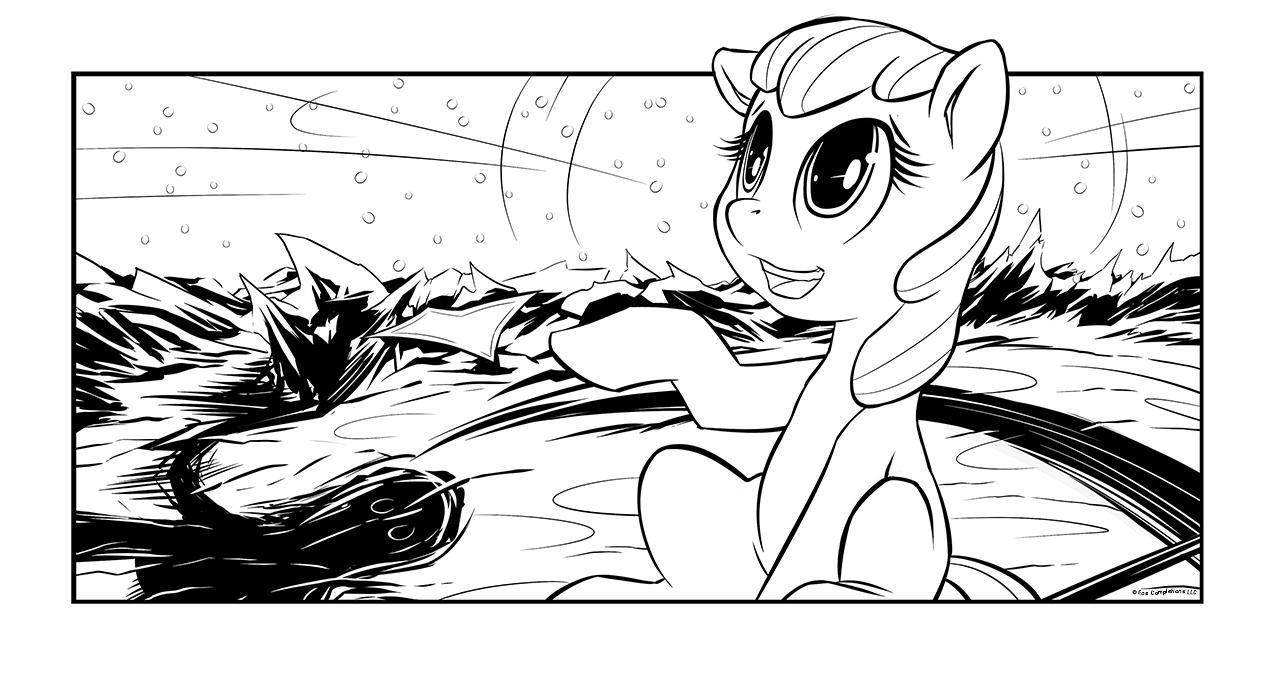
\includegraphics[width=0.9\linewidth]{image20.png}

\begin{intro}
And when the party's over we'll gather `round for a group hug!
\end{intro}

\englishdaytimeplace{14}{12:35 A.M.}{Emerald Shores, Big 52 S Branch}

Against the din of waves crashing into the rocky shore, Puppysmiles sat facing a gravestone. Her group of friends argued a short distance away, but she could only hear the Voice whispering inside her head. It spoke of pacts and promised dreams.

``Yes, yes, just\dots make all of this stop.''

Henrietta barely heard Puppy talking behind her, but she felt a sudden chill in the air, like a cold night's breeze, bringing with it the creepy sensation that she had just woken up from a bad dream but couldn't remember what it was about. Suddenly, what Puppy had said seemed a lot more important.

Everypony turned toward Puppysmiles. Was she talking with herself? Make what stop? How?

As Henri approached, she could see that Puppy's eyes were closed and her head hung low. Her mane was rapidly changing color, turning dark blue from its original blonde. ``Puppy? Are you okay? What\dots I\dots I think that you have something in your mane.''

When Puppy spoke, it was with a different voice. Like the sound made by a chorus of ponies calling from the bottom of a cave. ``I salute you, my humble minions. I'm finally here among you, bow at the dawn of a new era!''

Henri cocked her head and raised both her eyebrows. ``The what of a new what? Puppy, what's going on?''

Sidekick's eyes turned from red to blue, and it took up position on Puppy's flank, standing like a sentry. The creepy new Puppy continued. ``I am not Puppysmiles. I am Creepy Voice, a child of the Stars, and your new ruler. Under my guidance, a new Equestria will rise.''

Scold shook his head and looked over at Molten Gold. ``The Stars? Like in ancient zebra folklore? Those Stars?''

Scold's question was interrupted by Henrietta's laughter. ``Creepy Voice? What kind of name for a villain is that? I mean, really? Creepy Voice? Did you come up with that all by yourself?''

Puppy stepped back, with an embarrassed expression that rapidly shifted to anger. ``It\dots it is a name you'll learn to respect, fools! Now bow to me and return to your towns, announcing my advent!''

Trigger Happy snorted, stepping in front of the other ponies. ``Or else?''

The blue flames that burned in Creepy's eyes expanded until they completely filled her helmet. A blazing cobalt crown appeared above her head, and more blue fire sprouted from her back, forming a pair of ghostly wings. ``Or else, I will devour your souls!''

Happy hesitated, looking at her while Lonesome Pony muttered to Scold. ``Can she do that? Can she eat souls?''

Scold looked back at Lonesome and shrugged. ``How am I supposed to know that? If she really is connected with zebra dark magic, then it's possible. Only I don't think she's strong enough for that just yet.''

He raised an eyebrow. ``She isn't?''

``No, she's still manifesting, just look at how that fire of hers is flickering. I think I know how to stop this story before it even begins.'' Scold spoke in a very low voice while Happy kept the creature occupied. Molten Gold and Lonesome Pony listened to him with all their attention.

``I think that I can sever the bond that ties this entity and Puppy's soul together. Without a soul to feed on, Creepy Voice, uh, that creature, won't be able to manifest itself and will be banished.''

``So, what are you waiting for, an invitation?'' Molten asked impatiently.

``No, I'm not strong enough to do this on my own. It's a ritual, but it's long and complicated, and meant for unicorns only. No offense, Gold.''

Molten shrugged. ``No offense taken. So basically you're telling us that we are going to be fucked by a zebra demon with a foalish name?''

``Hey, what's going on? Does the egghead here have a plan?'' White popped his head into the trio of ponies, interrupting the conversation.

``Actually, yes, but I need some minutes to figure out the details, help Happy keep Creepy Voi---no, really, what kind of name is that?'' He facehoofed. ``Well, keep her talking while we try to pull this off, okay?''

White nodded and turned on his tail, trotting toward the trio composed of Henrietta, Trigger Happy and Jammed Gun. ``Hey, Your Highness, did you mention something about a new era? Can you elaborate on that part? Will it be better than the manure we are swimming in at the moment?''

The nightmare stopped considering Henri and her annoying question about names and turned toward the new arrival. ``Indeed! My magic is far superior to that of mere ponies, with it I can heal this poisoned land and bring about a new reign of prosperity! Your violent lifestyles will be at an end. I won't allow my subjects to squabble amongst themselves. Instead you will build immense temples in my honor! All you have to do is worship me, and pay tribute to me and all the problems in your life will be solved!''

White nodded at the response and tilted his head. ``Well, that sounds mighty interesting, but may I ask what you mean by paying tribute to you?''

She smiled before sitting down and closing her eyes, acquiring an air of mentorship. ``Absolutely. Your master, that is me, will ask very little for the good of many. Aside from your worship, I require a pony sacrifice every full moon from each major city. In return, I will cleanse the land poisoned by ponykind, allowing you to grow food and live your lives under my rule!''

Trigger Happy cocked her head, frowning. ``W-what are you going to do with sacrifices?''

Creepy Voice waved her hoof, dismissively. ``Never you mind.''

Henri and Happy had their mouths open, listening at what she was saying. Happy drew her weapon, but she stopped when she noticed White's gesture to wait.

Henri, on her side, scratched her head. ``Yes, but\dots will you give us back Puppy?''

The nightmare blinked her eyes for a moment, surprised. ``What? She doesn't want to come back. She is sleeping and dreaming, in a place where nopony can hurt her. We made a pact.''

At that reply, Trigger Happy snapped. ``You did a what? Listen, I know my friend Puppysmiles and how easy she is to trick! Whatever pact you made, it's not valid! You can't just\dots just talk a foal into something and pretend it's legitimate! Let her go!''

The nightmare laughed, with a silvery tinkling voice. ``Tee-hee, you're funny! Why should I yield a perfect soul to possess? Her obsession trapped her on this plane and as long as she sleeps, she will never realize the truth. So no, I'm not letting the foal out of her dream, but on the other hoof, I'm offering all of you the privilege of being my heralds so you can announce my coming to all of Equestria.''

``So, long story short\dots'' Henri tilted her head. ``You're Nightmare Moon?''

``Well, no\dots I mean, yes\dots I mean\dots Nightmare Moon was more ancient and powerful than me\dots'' For a moment the creature hesitated, but she seemed to recover almost immediately. ''But I am more than strong enough to shut your stupid beak!''

Henrietta deadpanned. ``So basically\dots you're a newbie. A Nightmare Noob.''

Trigger Happy burst into laughter, rolling on the grass as she fought for breath. Mister White facehoofed, while the other three ponies stopped talking for a moment, trying to understand what was going on.

``ENOUGH! THAT'S IT! THERE'S PLENTY OF SUBJECTS I CAN USE, I DON'T NEED YOU, USELESS BUNCH OF\dots OF IGNORANT WEAKLINGS!''

Henrietta snickered. ``Said the filly that can't count beyond four\dots''

``YOU INSOLENT LITTLE\dots YOU WILL SUFFER!''

``No, she won't! Bad monster! Stay put!'' Scold stepped in front of Henrietta, staring straight into the Nightmare's eyes. ``We will banish you forever, with the power of science!''

``Tee-hee,'' The creature giggled, evidently quite capable of shifting from anger to mirth on a whim, and dismissed the scribe with a wave of a hoof. ``Don't make me laugh! Science! Do you have the slightest idea of what power you are facing? Oh for Nightmare Moon's sake, try something more believable!''

Scold smiled, not very impressed by the nightmare's reaction. ``Oh, so you want the details? Very well, then listen carefully. Since I already had the opportunity to check Puppy's suit, I did some research and I found some interesting clues. Your very existence in this place is caused by a foolish attempt at using necromancy as a life saving device, but I know how to fix that horrific mistake the Ministries made! The talisman itself has proved to be almost impervious, but the spell inside is more than unstable. The way your flames wax and wane make that abundantly clear. Now, I have some unicorns here and even if they don't know a thing about dispelling magic, I can tap into their power for as long as we need. So, guess who's getting dispelled today?''

``What the\dots'' The demon stepped back, with an expression of real concern on her muzzle now.

``All right everypony, I'm casting the spell, you just clear your minds and this nightmare will be over! Let the magic flow!''

A flash of light exploded from Scold's horn and shot between the assembled unicorns, each of them sending out ethereal threads that became woven into a mighty spell.

Happy closed her eyes and let the magic flow through her, quickly followed by Mr.~White and Jammed. Soon all their horns were glowing a brilliant white and the light expanded until it had enveloped the whole hill and everypony on it.

Henrietta grit her beak tightly and was forced to shield her eyes from the blinding glare. Something that Scold had said didn't sit right with her. He was going to stop the demon by destroying the necromantic spell being used as a life saving device, but wasn't that what was keeping Puppy alive?

Henrietta turned toward the old scribe. ``Wait! Are you trying to kill Puppy?''

Scold didn't reply, but from within the shining cloud of light the monster's voice confirmed Henri's fears. ``Fools! If you break the spell, the foal will die with me!''

``No, fuck, NO! You're not going to kill her, you fucking unicorn!'' Roaring, Henri charged at Scold, slamming into him so hard he flew for a couple of meters before landing heavily on his back. He screamed in pain and lost focus on the spell.

The light exploded in a rainbow of colors, spreading all around and dancing in every direction, but without a pattern. It was more like a giant disco ball gone crazy and rolling along a corridor than a real rainbow, and when at last the light died\dots

Nightmare Noob opened an eye, uncertain of what was going to happen next. Everything seemed to be still and silent, so she dared to opened the other eye too, and looked at the confused ponies in front of her. An evil smile appeared on her now very satisfied muzzle.

``So, in the end, Puppy's griffon friend proved to be very useful to me. But next time you might want to pick better allies for yourself, yes?'' The nightmare chuckled. ``Oh, silly me, there won't be a next time, since now you're all going to die.''

Scold shook his head as he got to his hooves, still dazed by Henrietta's tackle. ``What\dots why did you stop the ritual, you featherbrain? It was working!''

The other unicorns looked around at each other in a stupor, struggling to stand after the exhaustion of casting. Molten Gold tried to wake Mister White, while Henri advanced on Scold, with a grim, accusing stare. ``You\dots you won't take Puppy from me! There must be another way, I'm sure of it!''

``But\dots you stupid deluded brat! The foal is already dead! We're trying to save the Big 52 here! Come down from your\dots your `wonderful dreaming place' and get real!'' Scold was practically foaming at the mouth. Henri had disrupted their best chance to win, and now a lot of ponies were going to die because of her.

The nightmare savored the taste of crushing victory that was still lingering in the air. ``Oh, this is so tempting\dots Looking at your little argument is a real treat, but I have a schedule.'' Creepy Voice looked at Sidekick and in that moment the ghoul's eyes turned night blue. Sidekick turned toward the ponies like a hound. Nightmare Noob smiled. ``Let the games begin. Go, my minion, teach that chicken some manners.''

Sidekick crouched, ready to pounce on Henri like a cat on a mouse. The griffon was so focused on her argument with Scold that she didn't notice the ghoul jumping until it was too late. She didn't even hear Trigger's warning.

The impact sent Henri and Sidekick rolled down the hill, a whirling ball of hooves and claws. Henri fought without thinking, her predator instincts being all that kept her from being crushed by the foal's unholy strength. She tore with her talons and punched with her fists, dodging the return strikes and knowing that a single hit would be the end for her. The melee continued, both figures locked in a dance to the death even as they tumbled over the edge and fell to the rocks below.

Creepy Voice watched as her minion vanished from sight and shrugged. ``Oh well, meanie chicken broke my toy. It seems that I'll have to do everything myself, as usual. So, who's first?''

Lonesome Pony and Molten Gold exchanged a quick glance before opening fire. They emptied their magazines at point blank range, the bullets tearing through the Nightmare like a hot knife through butter.

Dozens of holes dotted Puppy's chest but they didn't seem to have any effect at all. Many had already begun to close. ``It's hard to kill something that's already dead, isn't it?'' Creepy Voice giggled as she lifted Lonesome Pony with her magic and slammed him into the tree. The pegasus hit the trunk with a wet, crunching noise, and fell to the ground unmoving, his back bent in an unnatural way.

Not even checking to see if Lonesome was actually dead, the nightmare turned toward Jammed Gun. ``So, I reckon you're with the sweet mare there? How cute, you'll die together, like the protagonists of some cheap old play! Any last words?''

``Actually, yes.'' Mister White smiled a little as he interrupted Creepy Voice and levitated a radio from his saddlebags. ``Plan B.'' His eyes narrowed. ``We've got backup.'' With a sound like distant thunder, sniper fire blew apart Pup's helmet and ripped away one of her legs.

The wicked creature roared. Spreading her wings, she flew up into the sky and conjured lightning from the clouds. The bolt struck the ferris wheel like a hammer, heating the metal and weakening the last joints that still allowed it to stand. The gigantic metal structure creaked and screeched, before collapsing on the small building that Sage Brush and a couple of acolytes were sniping from.

``No! Sage!'' White turned toward the town, looking at the rubble that once had been his nephew's hiding spot. No, this was\dots this wasn't going as planned at all!

A salvo of missiles streaked through the air toward the creature when she was far enough from the ponies below, shrouding her completely within a flourish of explosions. The rangers charged from their hiding spots in town, discharging every weapon they had in the monster's direction.

The battle had begun.


\horizonline


Henri groaned. It was all dark, cold and wet. Her bones ached in places she didn't even know she had, and she was almost sure that something was completely wrong.

A sweet and merry voice hammered like a pink flash in her head. \emph{``Oh don't worry, it's just you being your usual meanie self\dots nothing else!''}

``A\dots meanie what? Am I dead?'' Her headache was getting worse, while the sound of explosions and ponies screaming thundered in her ears. There was a\dots a thingy, something like a pink dot, dancing in her head and speaking to her.

\emph{``Silly chicken, you're not dead, \emph{duh}! You're just a bit confused and somersaulting down six meters onto those rocks didn't help at all, but I'm sure you'll be okay lickety split! Dashie did that all the time and never got hurt!''}

``Puppy\dots how is she? I-I must save her!''

The pink dot moved a bit, shifting from a colloquial, merry attitude to a more accusing one. \emph{``Really? Because it seems to me that you're simply trying to hog her all for yourself!''}

``What the\dots what the fuck are you blabbering about? I just want her to be safe!''

\emph{``So that she can stay with you forever and ever?''} The voice started fading. \emph{``Whom are you wishing well? Poor little Puppy or poor lonely Henri?''}

``I\dots I don't know anymore. But I\dots I want to make her happy. She seems so different, like a distant memory that doesn't want to fade. I don't want to lose her, but she seems to be unable to think of anything else but her mother, like a\dots a recurring nightmare!''

\emph{``Or maybe a sweet dream that doesn't know how to fade. Maybe she just needs a last, little help from her very best friend.''} The voice had gradually changed. At first it had sounded like an overenthusiastic youth, but now it sounded like an old mare. Somehow it was very, very familiar to Henri, reminding her of the dreams she had had when she was prisoner in Sun City. \emph{``There's just one last step to trot. Find Puppy's rock and fulfill its destiny.''}

With a gasp, Henri opened her eyes, finding herself in the middle of a rocky beach. She was lying on what was left of a badly crushed Space Ensign Sidekick. The ghoul had taken the brunt of the fall and was now just a flat squashed yellow bug. Henri drew one of her .45s and made sure that the creature was completely gone, putting another two holes in its head before checking the surroundings.

Up above her head, a pony flew over the ridge, screaming as she was sent out to sea. The dark magic faded, and she kept going for a good two hundred meters before splashing in the cold waters.

Henri tried to ignore the sounds of battle coming from above her head and gulped down a healing potion as she began her search for that stupid stone. ``Puppy's stone, Puppy's stone, how the fuck am I supposed to find a damn stone in the middle of a rocky beach? Magic Rock my ass!'' She scowled at a nearby rock and kicked it hard, sending it flying into a rusted metal box a few meters away. The rock rebounded and, of course, hit Henri squarely between her eyes.

``Fuck!'' She rubbed her forehead and picked up the offending stone from the ground. Every rock had its voice, and Henri knew this one very well . ``That's the last time you get one over on me. So what now? You hit a metal box, dumb rock, were you trying to tell me something? What are you, some sort of rock of destiny?'' Henri snickered as she approached the box, and introduced its padlock to \emph{The Rock Of Destiny}.

``At least\dots''

\emph{CLANK!}

``You're being\dots''

\emph{CLANK!}

``Useful!''

\emph{CRACK!}

``Very well, let's see what's inside the treasure chest.''

Some papers, an old brushable Applejack doll, some photos\dots Henri took the pictures and looked at them. In one there was Puppysmiles, only younger and without her radsuit. She was smiling in front of a carrot cake with four candles on it. There were some other ponies in the background. It seemed to be a birthday party. On the second picture there were a white stallion and a purple mare, and they were sitting in front of an old wooden sign announcing that they were entering the town of Appleoosa. Between the two ponies sat a pouting Puppysmiles, as if she didn't want to take the photo or be in that place at all. She seemed even younger in this picture, maybe three. Henri turned the picture and found a note: \emph{Last trip with Better}. A third photo showed Puppy dressed in a smock, and sporting a big blue bow in her mane. She was smiling, proud of her new dress. Another note, written on the front this time, said: \emph{Puppy's first day of kindergarten}.

Turning the last photo, the young mercenary found some weathered lines written on the back.

\medskip

\emph{In a different place and in a different time, beyond the horizon, we will be together again with Dad, and I'm sure I'll be proud of you.}

\emph{Because Mom will always be proud of her little sunshine.}

\emph{I love you.}

\begin{flushright}
\textbf{Mom.}
\end{flushright}

\medskip

A missile flew over the ridge and exploded on the shore, illuminating just for a moment the tears running down Henri's face.

Henri sighed, finally giving in to the truth in front of her eyes. ``She\dots she never belonged here\dots Fuck.'' Henrietta rubbed her eyes, putting down the photos. ``Fuck, why does it have to end like this? WHY?''

A new explosion painted the sky red. Ponies up there were dying, fighting something that was already dead. Dying because she wanted to keep Puppy for herself instead of letting her go, as it should have been. Now Henri knew what had to be done. Still, that didn't mean she had to like it. ``Not fair. Not fair at all\dots''


\horizonline


Paladin Gauss's eyes widened as the missile he'd just fired was thrown back at him.

``Gauss! NO!'' Cold Shower could only watch in horror as the explosion took away one of her oldest friends. She turned toward the Nightmare, her eyes full of anger and pain. ``Stupid bitch, why won't you die?'' The barrels of both the miniguns mounted on her power armor span up and she fired until her guns were empty, but the bullets bounced harmlessly off the nightmare's shield and were completely ignored as the creature launched a second acolyte into the ocean.

Creepy Voice had already killed two rangers and thrown several other attackers onto the sea, but with all these ponies around she was getting confused. How was she supposed to fight all of them at once? Really, these stupid equines didn't even know the rules of a proper duel! She was growing bored of their little game. Yes, killing ponies could be fun, but it seemed pointless, especially when she had more important things to do, like take over the world.

Who was supposed to be the leader of this bunch of idiots? Oh right, the old scribe\dots Creepy Voice smiled with evil on her mind. ``So, where is that guy with the cape?'' Landing in front of the old pony, Creepy Voice folded her ethereal wings and faced her adversary, not even trying to hide her amusement. ``Here you are! Scold, right?'' There was a pause, while he looked confused at her new change of mood, but the nightmare cut it short. ''Very well, die.'' With her magic, the monster grabbed his heart and squeezed. Scold collapsed with barely a whimper.

In the same moment, Henrietta flew over the ridge, landing again on the tomb's hill. The scene in front of her eyes made her cringe. This was her fault. All of this was happening because of her selfishness. Ponies fighting, ponies dying, this wasn't what Puppy would have wanted at all. It was time to end it. ``Puppy! Puppy, listen!''

The nightmare let out an annoyed sigh and turned toward Henri. ``Hey, it's not your turn yet! Don't you know that there's a list? I'm almost finished with this one, then I'll be killing you too, so don't push and keep your ticket ready!''

Trigger Happy crawled toward Scold while the nightmare was busy giggling at her own humor. Happy tried desperately and uselessly to revive the scribe. Their numbers were being mowed like a wheat field in front of a reaper. Molten Gold was struggling to break free from the tree he had been impaled on, Lonesome Pony had already passed out with his back broken and even the well equipped and combat trained rangers were losing ground. This was the end. They were all going to die here. For a moment, Trigger felt sad, she really, really wanted a foal of her own to love and care for. 

``Puppy, wake up! You\dots You can see you mother for real!'' Henrietta kept screaming with her high pitched bird voice. She was actually quite annoying. ``This Nightmare is a bug and a stinker! You're cooler than that! You learned from the best!''

Creepypup snorted. ``Aren't you even able to wait your turn to die?'' A halo of dark magic surrounded a large chunk of road and hurled it toward Henri, but she was agile and dodged it easily. ``Now I am disappointed, bad chicken! Do not make me come down there!''

Henrietta flew in front of Puppysmiles and pressed her beak against Puppy's glass helmet. ``Puppy, you moron, you are dead! D.E.A.D.! Just like your mom! Are you so stupid that you don't even realize how to die? Dump this idiot and go with your parents! Please!''

``What?'' The nightmare blinked her eyes, startled by Henri's sudden assault. What was she saying? Was she trying to speak to Puppy? Oh no, no no nononono! ``Shut up! She can't hear you, fool!''

``C'mon Puppy, wake up! You're not forced to stay here! I\dots I don't want you to stay here with me, you have to go! I'll be fine! Just\dots''

Henrietta was trapped in a blue corona and her body started to twist, producing disturbing snapping sounds. Creepy Voice looked straight into Henri's eyes, with a stare full of anger and hate. ``You. Die. Now.''

Henrietta smiled weakly, unable to resist the powerful magic crushing her body. ``Puppy\dots Mom is\dots just over the horizon.''


\horizonline


Puppysmiles sat in front of a pond, looking at the fishes that swam within. Everything around her was still and calm. A blanket of snow covered the ground and the clear sky showed hundreds of stars. She wasn't happy, but somehow she wasn't sad either. It was like being dazed, everything seemed so muffled and unimportant. It was just her, the snow and the fishes in the pond.

Puppy wasn't aware of how much time passed since she sat there, but it wasn't so important. She just wanted to forget\dots she couldn't remember. Well, maybe it was actually working. At least, until a weird goldfish poked its head out of the water.

``Puppy, you moron, you're dead!''

``Wut?'' She tilted her head, then checked her hooves and her tail. ``I'm not dead, stoopid fish!''

A second fish poked it's head from the pond, this one spoke in a feminine voice. ``C'mon Puppy, wake up! You're not forced to stay here!''

``Henri? Why are you a fish now?'' Puppy giggled. ``Silly Henri, fishes don't talk!''

Frost began to creep over the pond, but a third goldfish jumped out from the water, talking again with Henri's voice. ``Mom is just over the horizon!''

\rcpr{``Mom, where did Dad go?''}

\rcpr{``He's somewhere beyond that rainbow, Puppy.''}

\rcpr{``Will\dots will he come back?''}

\rcpr{Mom didn't reply, but Puppy really, really wanted to see Dad again.}

\rcpr{``Can\dots Can we go where he is?''}

\rcpr{``Yes Puppy. One day, maybe not tomorrow, or not the day after\dots In a different place, and in a different time, we will be all together again, okay? Just\dots just over the horizon.''}

\rcpr{``Pinkie swear?''}

\rcpr{``Cross my heart, hope to fly\dots''}

``Stick a cupcake in my eye\dots'' Puppy looked up in the sky. And finally saw him.

``---really, really late and I know I actually have all the time in the universe, but I hate these kinds of anomalies, and this one has been going on for two hundred years! I'm beginning to lose my cool, because there are a lot of better places I'd like to be rather than here!'' A skeleton wearing a black hood was talking in Puppy's direction, but he seemed to talk to himself more than her.

She smiled. That skelly pony was funny, he was talking like those grumpy ponies at the veteran retirement house! ``Hi, I'm Puppysmiles! Have you seen my mom?''

``Oh, please! Not that litany again! I'm going to resign, or strike! Or strike and then resign!''

The skeleton pony was interrupted by the giggling Puppy. ``Tee-hee, skelly pony is funny!''

Stopping his monologue, the grim reaper finally noticed that she was looking at him. ``You\dots can you see me? Is this some sort of prank? Because if this is a prank, I'm going to give up for real this time.''

Puppy tilted her head. ``A prank? I hope not! Last time I made a prank I was spanked ultra hard!''

The pony paused for a long moment before falling down on his haunches with a ghostly sigh. ``At last\dots''

Puppy trotted near to the weird looking stallion and sniffed his clothes. ``Ah, who are you, pretty skelly pony?''

``Me? I'm the Grim Reaper, Death, the Inevitable End, the Black Stallion\dots'' From Puppy's blank stare, the skeleton realized that he was just wasting good words. ''But my colleagues call me Mort. Long story short, I'm the guy that shows the deceased how to reach their afterlife.''

Puppy tilted her head, confused. ``So\dots Have you seen my mom or not?''

The skeleton shook his head. ``You're a lost cause.'' A silvery ticket covered in shining pink letters appeared in front of Mort and gently fell like an autumn leaf between Puppy's hooves. ``Here, take this ticket. It's worth a ride to the other side. Remember, not everypony gets the silver ticket. It's a really special one that will bring you there lickety split, so be grateful.''

Puppy's eyes grew bigger. ``I\dots I am going to see Mom? For real? No more pink arrows, or stoopid bullybots, or falling houses? Just\dots Mom?''

Death nodded. ``Exactly.'' Mort paused for a moment before continuing. ``It must have been hard. This is my personal way to say I'm sorry for not being able to help you earlier.''

Puppy stopped listening as soon as the pretty skelly pony had said what she wanted to hear. ``Yush!'' Puppy hugged Death for a moment, before looking at the pond which had now completely frozen over.

``Oh right! Henri! Just let me say bye to my friends!'' Puppy turned on herself and the whole scene with the pond and the snow exploded into a thousand shards, dissipating into nothingness and revealing the battlefield around the graveyard.


\horizonline


``\dots Just over the horizon.'' Henri's eyes grew clouded as she slipped into unconsciousness.

As soon as Henri had said those last words, the Nightmare's eyes flared pink and for a moment her expression changed completely. ``Bye bye Henri! A pretty skelly pony is sending me where Mom is, and this time with a super shiny ticket!''

The pink in Puppy's eyes faded away one last time and all the lights on her HUD turned red, signaling an endless sequence of system errors.

{\mten ``Warning. Subject 001 Puppysmiles cannot be located. Warning. Power level is critically low. Warning. Self repair function not responding. Warning. Hardware not found. Warning. General shut down in five, four, three, thank you for using Ministry of Peace technology. Have a nice day, and please, be safe.''}

With these words, the whole HUD on the helmet disappeared, leaving only the shocked face of Creepy Pup staring at the now empty glass.

The monster stepped back in horror, releasing her magical grasp on Henri, who fell to the ground and rolled a few meters downhill. ``What have you done, fool? I'll kill you all immediately, puny insects!'' The monster stretched her wings, ready to release a new wave of magic, but something was wrong with her. The suit had begun to deflate like an old, empty leather ball. ``What\dots what's going on? I'm melting! NO, NOOOO!'' Small eruptions of pink gas leaked from every hole in the fabric, while the monster fought to keep her grasp over what was now an empty husk.

``You! You have not won! I will be back! Ponies make the same mistakes all the time! I'll be baaAAH---'' Creepy Voice's face melted in a pink eruption, filling the helmet with a curtain of gas. For a moment the suit inflated like a party balloon as whatever force that kept the pink ooze in a fluid form stopped working and the pink agent reverted to its usual gaseous state. As the scream from the Nightmare reached its highest note, the suit's locks failed and the gas exploded out of the harness, making a sound like a whistle.

The ponies that still were capable of walking grabbed the wounded and dragged them away, far from the expanding cloud of pink death that had started to lazily invade the whole hill.

``Go go go! Let's get away from that stuff!'' Cold Shower dragged away what was left of Gauss, following the others.

Creepy Voice continued to scream as they fled, a long wail of anger and agony.

Half dragged and half pushed, for a moment Henri regained a spark of lucidity. Everything seemed distant, and she felt as if she was floating in a warm place, lulled by gentle invisible waves. And in the middle of that moment of peace, she heard Puppy's voice. ``Hey, hey Henri\dots''

Henri groaned. That foal wouldn't know the difference between a wrong moment and the worst possible moment even if she bumped into it with her muzzle.

Puppy ignored Henri's mental complaints. ``Listen, I has really no time, but I wanted really really REALLY to say I'm sorry, but I has to go\dots I\dots we are still friends, right?''

Still friends? That was a weird question. Puppy was more than a friend, she was something more, something bigger, in Henri's life\dots

``Really? You\dots you liked me that much? I know! We can be sisters! Yush! Henrietta Days! I lovelovelove it!''

Henri chuckled, still half dazed by the Nightmare's embrace. Henrietta Days\dots Sure. That was totally going to happen\dots Adopted by a pony.

``Okay sis, gotta go I love you bai!'' And with those last words Puppy's voice faded away as the griffon passed out again.


\horizonline

\englishdaytimeplace{14}{17:00 P.M.}{Emerald Shores, Big 52 S Branch}

\rtpr{Good day, Big 52! And for once I mean it! This is DJ Good Stuff and you are listening to Radio 52, the radio of good news!}

Boisterous triumphant music played for a few seconds.

\rtpr{I've been receiving transmissions from Ironworks and Broccoli since this morning and now I can safely say that the news is confirmed: the Wild Herd was defeated! WOOHOO! Yes my little ponies, you heard me well, the good guys trotted down to Ironworks and kicked some raider ass for good!}

The DJ laughed enthusiastically, evidently too happy to keep even a shade of professionalism.

\rtpr{I still lack the details, but it seems that the Applejack's Rangers along with a group of volunteers, and please note that Lonesome is among them, assaulted their camp very early in the morning and caught them by surprise, killing a large number of raiders and routing the others. This is how things get done `round here, raiders! You better think twice before you mess with us!}

Good Stuff paused for a moment before continuing; in the background there was a sound of shuffling papers.

\rtpr{Okie dokie, now, for those that have friends and relatives in Ironworks\dots The situation seems dire. Most of the adult ponies have been killed during the siege, but there are still some survivors, mostly the elders and the foals, with a small group of guards that found shelter inside Ironworks's Stable. I don't have a list of the survivors so far, but I'm working to get one, so expect some more news during the day.}

\rtpr{In the other news, Splendid Valley was hit by a huge explosion that completely devastated it. Apparently, this has something to do with the Enclave, since---}

Trigger Happy turned off the radio and turned toward the Hill. The pink cloud had been scattered by the wind, but not before coloring the solitary tree in sugary pink. Right under the tree stood two graves.

Henri looked at the last stone in her claws: \emph{The Rock Of Destiny.} She sighed, weighing Puppy's weapon before putting it on top of the small mound erected next to Rainy Days's grave. A small toy pony sitting on a foal-sized red scooter had been left in front of the memorial, almost like a bunch of flowers.

She opened her beak, looking for some words to say, but closed it again without thinking of anything. Mister White arrived from town, carrying a rusted road sign. The stallion patted Henri on the shoulder before taking a brush and painting two words on the metal plate. 

\begin{center}
	\textbf{---Puppysmiles Days---}
\end{center}

Trigger Happy approached the new grave, frowning a bit. ``Is\dots is that all? Just a name? It seems so\dots cold.''

He shrugged. ``It's how we have always done things `round here. Graves are not for showing.'' White looked away from Trigger, staring at the other graves on the hill. Cold Shower and Scold still sat in front of the numerous ranger graves. Sage Brush's tomb was sitting alone, facing north, toward Salt Cube City. White shook his head and turned back to Happy. ``It wouldn't be fair. Her grave is not the only one that was dug today. Let's stick to our traditions.''

Trigger Happy nodded and sighed before she turned away and approached Scold. The old unicorn was looking at a holotag in his hooves, but when the mare approached him, he put the object away with a sad expression. Happy kept her voice as low as possible while talking to him. ``How are The DJ and the Ghoul doing?''

Scold shrugged. ``Gold will survive. He just needs some radiation. Lonesome Pony\dots well, we will try implanting him with an artificial spine, but we lack the correct instruments, and I don't know if he'll survive the operation. Your coltfriend should be with him right now, so maybe you should go and check yourself.''

She lowered her eyes. ``I-I'm sorry for your losses\dots I could have taken all the guards from Tunnel Town with me, not just me and Jamie\dots''

The old scribe smiled weakly. ``It's not your fault, we had no idea of what we were going to face here. Those that gave their lives fighting against that horror will be remembered as heroes. I know it won't bring them back, but maybe this will give at least some meaning to their deaths.''

As soon as Trigger Happy departed, Scold trotted next to Cold Shower and sat with her in front of Gauss's tombstone. She was crying in silence; the two ponies were more than comrades, and the loss had been a bad blow for her.

``He was a good friend\dots You know, even when he acted like an ass.'' Shower was having a really hard time, trying to hold back her sobs as she spoke.

Scold nodded, wrapping a hoof around the mare's neck. ``Yes, he really cared about ponies. He knew what was important\dots'' His stare wandered across the graves. Four. Two paladins and two acolytes. The Rangers probably owed Puppy more than that, but it felt hard to accept it. Still, he didn't want to blame the griffon for that, it simply didn't feel right. ``We lost many good ponies, today. Acolyte Sugar Flavor and Scribe Scroll were still so young. I'll have to inform their parents.''

Cold Shower sighed, tears now running down her muzzle. ``Scold, please\dots{} Tell me it was worth it. I lost so many friends\dots I lost the pony I loved. Tell me\dots tell me they didn't waste their lives.''

``We are just ponies, Shower. We do what we can to make this land a better place day by day. The records say that in the last generation, in the Big 52's settlements cutie marks involving traditional works like masonry, farming and arts are slightly growing. Maybe things are getting better, and maybe our foals will see a greener Equestria.'' Scold looked at Puppy's grave. ``And maybe, one day, there will once again be a place where foals like Puppy will be free to play and make friends. Who knows\dots''

Henrietta rubbed her eyes as she left Puppy's grave and trotted toward the beach, looking at the waves. Henri checked that nopony was looking at her, and when she was sure of being alone, she took Silky Tail out from a bag, hugging the doll and hiding her face in the pink plushie. 

``Don't worry, sis. Tomorrow will be a better day.''

~\vfill

\begin{engnote}
		Level up! (20) No wait. You're dead. Sorry kid, better luck next time.
	
		New Quest Perk unlocked: Filly Luck - Requirements: Level 8, Minimum Luck of 7. ``All right, we were just surrounded, okay? And the droids were all over the place, got it? And we got, like, five shots left, okay? Then all of a sudden, we hear a ruckus from downstairs, and the next thing we know is that half the robots were brutally demolished piece by piece by Celestia-knows-who! With a stone! Real story, man, honest!'' Occasionally, when facing robots or feral ghouls, you can find some groups of them already dead, brutally killed with a stone. Go Puppy!
\end{engnote}




}


\ctexset{
chapter/aftername = \quad,
chapter/titleformat = \huge,
chapter/format = \huge\bfseries\centering
}


\ctexset{
part/name = {第,部分},
part/number = \chinese{part},
chapter/name = {第,章},
chapter/number = \chinese{chapter}
}

\pagestyle{chinese}

\part{中译版}

\chapter{避风港}

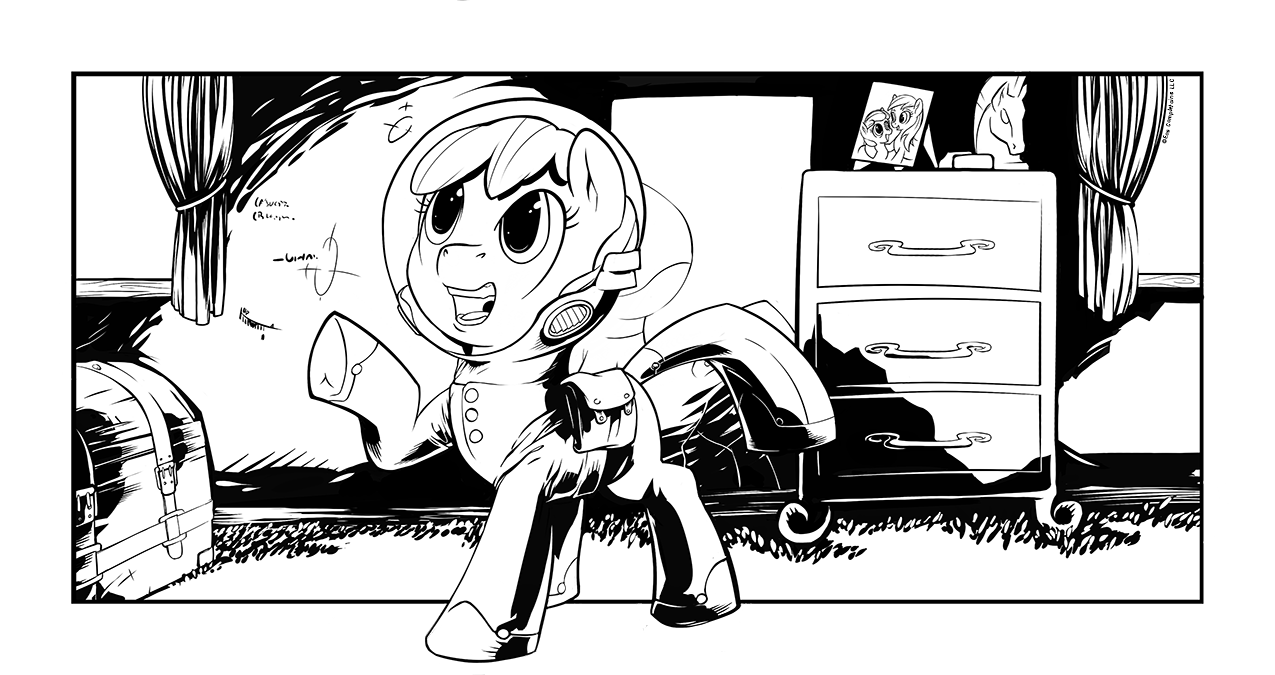
\includegraphics[width=0.9\linewidth]{image01.png}

\begin{intro}
    你相信幽灵吗?
\end{intro}

「拜托让我们上车!防护罩要失效了!快没时间了!」

长长的一大队小马焦急地等在一辆天空马车前,但是却没有看到拉车天马出现。忽然队末的一只绿色独角兽雌驹疯狂地推着马群尖叫起来。

「这不可能!这不可能!怎么可能会这样!?赛拉丝蒂亚抛弃了我们!露娜抛弃了我们!这……」

砰!

慌乱的雌驹无声地倒在了地上,所有小马齐刷刷转头看过去,卫兵正在将子弹压入霰弹枪。

「整整齐齐站成一排!排好队挨个上车!谁找麻烦我只好用致命手段了!」

中心城的塔楼之下穿行着惊慌而绝望的马群,它们将成为这场歇斯底里的疯狂毁灭行为的见证者。

\horizonline

远处上方中心城的街道上,小马们发疯一般争先恐后地寻找庇护。整个街区都被大火吞噬,许多道路都被翻倒的马车、破碎的建筑物和一些残垣断壁堵住了。但还有一些小马试图互相帮助,努力清理道路并救助伤马。

在一条拥挤的街道上,一群种马试图破开一堵残损的墙。

「再来!大家一起!使劲儿!」小马们再次用力向墙上尥去,爆发出自己全身的力量。

终于,墙屈服了,塌出了一个大家都能通过的缺口。除了一只年轻的小雌驹不知道发生了什么以外,这条路已经空了。她坐在街道中间,眼睛盯着她的鬃毛,接着又盯着天空。远处,一个巨大而闪亮的泡泡包裹着整个城市。在她盯着泡泡看的时候,有些东西击中了护盾的顶部并爆发绚丽的光芒。

「哦,耶!烟花!」她高兴地喊了出来。

「嘿,那边的小鬼!」

一个穿着白色制服的独角兽医疗兵正在给幼驹发放防护服。在看到这只小雌驹的时候,她冲了过去,露出了令马担忧的表情。

「就你自己吗?你家长哪儿去了?」

幼驹对着医官微笑着。「妈妈在那上面!」她用蹄子指着中心城的闪光防护罩,防护罩现在看起来比10分钟之前薄了很多。「她晚餐的时候就会回来!」

士官踌躇了一下,然后对幼驹勉强一笑。「当然……她会回来的。小家伙你叫什么名字?」

「我叫快乐帕比(Puppysmiles)!」幼驹开心地蹦蹦跳跳着。

「好的……好的……帕比,没关系……你仔细听好,穿好这件外套,不管发生什么事情,都不要脱下来,好吗?」

幼驹有些疑惑的视线在黄色的东西和白制服独角兽之间来回转了转,「好的,漂亮的大姐姐!我喜欢你!」

独角兽紧张地笑了笑,然后漂起并展开了防辐射服:那是一件柠檬黄色外套,蹄子上有几个口袋,体侧还各有一个鞍包。

「好,你要把你的蹄子放进这些洞洞里面,就像是……像是……小马舞一样!你知道小马舞吗?」

「当然!」

% NOTE: 遵照英文发布版改

\begin{song}
    「右蹄伸出去
    
    右蹄缩回来!」
\end{song}

「对对,就是这样!然后是尾巴……好了,然后让我给你密封好,最后是把这个放在你的头上……好了!」

雌驹把一个原型的玻璃头盔戴在了帕比头上,然后把两边的卡扣锁紧,把孩子安全地包在了她的防辐射服里面。

「哇塞!我看起来就像是个太空小马!就像是……像是安德洛队长一样!呜!!!」幼驹兴奋地蹦来蹦去,白色的雌驹微微松了口气,然后转头走向下一队幼驹。

快乐帕比觉得现在真开心极了。一个巨大无比的烟花爆炸了,它听起来像一个非常棒的派对礼花!城堡被超大的肥皂泡泡包着,就像是妈妈用肥皂吹出来的那样,不过要大很多很多。大家都像在大庆典之前一样走上了街头。她偷偷对自己的幸运星祈祷妈妈能够早点回家,这样今天她就能和妈妈早点在一起玩耍了。而这个超级酷的太空服更是大大的意外惊喜,看来大家都想把她打扮得漂漂亮亮的,然后……对了!现在她需要面镜子!小雌幼驹毫不犹豫地跑回家去。

\horizonline

在她妈妈的卧室里面依稀听得见街上喧闹的声音,帕比站在梳妆台之前,仔细看着她的头盔,她面前出现好多奇怪的发光符号和文字。不管她看向什么那东西就会被一层奇怪的绿光笼罩,然后下面出现一些小字……可惜的是帕比认识的字不多,她妈妈还没怎么教她。

「嗯……唔……这个字是……」幼驹皱着眉头看着那个字,「床!哇哦,我好厉害!」

帕比得意洋洋地走下楼,完全把镜子的事情忘在脑后,转身打开了冰箱。

「马芬!」

帕比拿起托盘正准备咬,但是却发现一个问题——她带着这个笨头盔根本吃不到……{}

「好麻烦……坏头盔!我该怎么把你拿下来?」她用双蹄抱着那个倒扣在自己头上的鱼缸用力扯了好几分钟,但是那东西纹丝不动。她气喘吁吁地坐下来,然后祭出了她的王牌。

「哇啊啊……」

大哭的时候帕比没注意到,一个红色的符号出现在视野下方。但是她的哭声被这件外衣的奇怪机械声音打断了。

「{\mt 主体状态——恐慌!}」

幼驹傻傻地眨了眨眼睛,发生什么了?谁在说话?

「唔?」

「{\mt 开始内部医疗检测。错误。系统重启。请等待……30秒。}」

这些话很有趣,但是对于帮她脱掉头盔却一点用也没有。帕比依然很不开心。

「走开,笨笨说话衣服!我要吃马芬!」

「{\mt 重启完成。检测版本。开始……十秒钟后检测结束……八……七……}」

在那一瞬间,外面的噪音变得更大——空气中从充满了尖叫声和哭喊声。帕皮觉得可能是外面的小马在唱歌。

「{\mt 五……四……三……}」

忽然整个世界都变成了粉色。幼驹可以看到窗外似乎有一个巨大的黑影降落在城市上空,就好像一个巨大的粉色棉花糖云从天而降,它似乎在一瞬间便吞没了街道,房屋和所有的小马。完全不知道发生了什么的帕比紧贴着玻璃窗,很好奇窗外有什么异变。

「{\mt 二……一……系统重启完成。开始自检。警告,主医疗护符\footnote{主医疗护符(Talisman):辐射小马国(Fallout Equestria)中设定的一种可以施展固定法术的的蚀刻符文。}没有响应。启动备用医疗护符。开始诊断。雌性,幼驹,陆马族。}」

哇哦,这个太空服真聪明!他知道的可真多!

「嗨,我叫快乐帕比!」

粉色的浓雾像毯子一般整个覆盖在了街道上,模糊不清的尖叫声变成了咳嗽声,小马的声音随着云将他们杀死或者变成更糟糕的东西而渐渐变弱。

\mtpr{「生命维持系统上线,体温正常,血压正常。警告,辐射水平超过正常水平300\%。」}

帕比咯咯地笑着:「咦嘻,太空服先生在说些听不懂的话!」帕比茫然地站在窗前看着正在漏进屋内的奇怪粉雾。她不知道……{}

\mtpr{「警告。检测到小量辐射毒性。注射:抗辐剂\footnote{抗辐剂(Rad-X):增加辐射抵抗能力},注射:辐特宁\footnote{辐特宁(Rad Away):清除体内辐射},注射:辐……」}

\mtpr{「 警告,危险药剂侦测,分析中。粉色药剂,幼角型\footnote{幼角型:Littlehorn type,或者下文的 Littlehorn agent 都是 \emph{FoE}(\emph{Fallout: Equestria})中粉雾(Pink Cloud)的「小马国官方」说法。}。浓度超过5\%可能致命。」}

「{\mt 1.8\%……2.0\%……2.2\%……警告,粉色药剂超过安全上限,建议立刻离开该区域。}」

帕比盯着地面上弥漫在蹄子间的粉色迷雾,看起来就像是棉花糖……粉色的棉花糖!

耶!自从上次噩梦节(Nightmare Night)她吃棉花糖吃到吐之后,她妈妈就再也没让她吃过。

% NOTE: 漏译,补上

突然,她感觉肚子收缩了一下。

「我觉得好好玩……」

「{\mt 危险!检测到变异产生!浓度达到 5.4\%。危险!6.0\%!请立刻离开!请立刻联系和平部\footnote{和平部(Ministry of Peace):小蝶创建的部门,主要负责健康事务和医疗方面的研究。} 获得救治!开始发送求救信号。扫描应急信道。发送中。警告,浓度达到 7.5\%}」

「呃……妈妈……我觉得……不太舒服……明天可以……请病……」幼驹面前的一
切都变得雾蒙蒙的,她觉得自己出了好多汗,但是又冷得像掉进了冰窖。

「{\mt 注射:治疗针(Med X),注射:治疗药水\footnote{治疗药水(Healing potion):\emph{FoE} 设定里的一种魔法药水,可以治疗大多数轻度伤病。}。浓度达到 12.1\%。注射:抗辐射药,注射:辐特宁。检测到粉色药剂浓度达到 16.0\%。注射:解毒药,注射:治疗药水,注射:治疗药水。浓度达到 22.6\%。注射:治疗药水,注射……}」

冗长枯燥的防辐射服医疗系统声音不断地重复着,一直到帕比的四蹄再也支撑不住自己,她失去意识,倒在了厨房地板上。充满她静脉的治疗药只是勉强延长着她的生命,致命的粉色药剂云雾正慢慢吞噬着防辐射衣,而医疗系统正在竭尽全力保证幼驹的性命,她还没有死,但是却不可能活下去。

「{\mt ……治疗药水,注射:治疗药水,注射:治疗药水,注射:治疗药水。警告,治疗药水剩余:3。检测到粉色药剂浓度达到 35.0\%。注射……}」

帕比就像一个被遗弃的玩偶那样躺在那里,衣服的声音还在不断报告着危险气体地渗入。最后衣服也放弃了,因为医疗药品已经耗尽。她再也没有听到那个声音。一个小时,两个小时,一天,两天……

幼驹只是躺在那里,穿着一件聒噪且唠叨不停的防护服,它只是在不停地提醒着幼驹她几乎要死了,而她需要……所有东西才能救她。

一天天过去,一周周过去,一月月过去。帕比还是那样安静地睡着,静止在她生命中的最后一刻。

几个月变成几个季度,几个季度变成几年,衣服还是不停地唱着它的摇篮曲。

几十年过去了,衣服的声音也越来越低,开始沙沙作响,被尘土覆盖的透明头盔好像是为睡个长长午觉的幼驹拉上安眠的窗帘。雌驹尘封在小小衣服中,被厚厚云雾笼罩,几十年慢慢变成一个世纪……两个世纪……

年久失修的房子开始慢慢风化,这是一栋非常坚固的房子,由陆马用传统办法一砖一瓦盖起来的。但是任何东西都有它的寿命,它开始因为春雨洗刷屋顶而发生裂痕,而夏天的每一场暴风雨侵袭,都让这小小的裂痕在慢慢变大。终于整幢屋子寿终正寝倒了下来。

正好砸在了小小快乐帕比的头上。

\horizonline

\daytimeplace{1}{5:00 PM}{四叶天台,中心城郊区}{Clover Leaf Terrace, suburb of Canterlot}

当坍塌的屋子消失在一片尘土和粉色烟雾之中,一切又重新回归了寂静。尘埃慢慢落下,在废墟之下却冒出了一个含糊不清的小小声音。

「好痛哦……」

慢慢地,一块砖动了动,然后是另一块,在碎石之中冒出一个闪闪发光的东西,一个圆圆的玻璃球头盔冒了出来,然后是一个穿着黄色防辐射服的小小身影。那头盔上有一道长长的裂痕,但是当幼驹从倒下的房子里爬出来的时候,那个裂痕就神奇地消失了。

「妈咪?」幼驹就像是一个踏上未知星球的宇航员一样。「这是哪里?大家都去哪了?妈咪?妈咪……?」

好像有什么不对劲的地方,她觉得自己还穿着那个会讲话的衣服。

「妈……咪……!」

「{\mt 兹兹……沙沙……线路……必须……重启……}」

「安静啦衣服!妈妈去哪了?房子去哪了?我到底……」幼驹抬头的时候把下半句憋了回去,因为在山顶之上的城堡废墟,是她绝对不会认错的中心城——她的故乡。

「什么……怎么……怎么坏成那样!」

「{\mt 吱吱……严重错误……没有组件……区需要去去去……启启起起起起……}」

「好吧,随你吧!」幼驹叫着,她看着头上中心城的废墟。忽然那种奇怪的感觉又来了。最初是她的视线变得模糊不清,然后她一屁股坐在了地上,她的蹄子都站不稳了,她觉得越来越虚弱,有一股剧痛穿过她的脊椎。那是一种奇怪的感觉,她的全身好像都停止工作,小幼驹想要大声尖叫,但是嘴都动不了。她唯一能做的事情就是在剧痛之中透过满是灰尘的头盔看着街道。

她只能坐在那里,看着一堆奇怪的灰白色肮脏石块,有大有小,有直有弯。现在她才注意到那些东西到处都是,不过很快一个绿点闪过她眼前,引起了她的注意。

「{\mt 系统重启完成。检查版本。未找到文件。启动应急模式。版本0.2……}」

帕比想说点什么,但是她还是完全麻痹,幼驹只是盯着眼前的那些奇怪的光点由绿色变为了粉色。嘿,终于有点儿好消息了,至少,她喜欢粉色!

「{\mt 发现新硬件。初始化矩阵。连接中。}」

火花穿过了幼驹的整个身体,从鼻尖到尾巴尖,冲走了全部麻痹的感觉,幼驹有些迟疑地举起一只蹄子,发现完全没有难度。然后她又走了两步,没有问题!就好像5分钟前的事情完全没发生一样,一瞬间医好了。

「哇哦,真奇怪……现在我只要把这个笨笨的太空服脱掉……」

「{\mt 全系统正常运作。开始例行监测。分析中。目标001,快乐帕比,雌性,幼驹,陆马种族。未发现内脏。检查系统错误,未发现错误。继续进行检查,雌性,幼驹,陆马族,无内脏。}」

「吴奶藏是什么?我想要!好吃么?」

「{\mt 读取幼驹学习程序。连接到印象部\footnote{印象部(Ministry of Image):瑞瑞在大战时创建的部门,负责形象设计与战时宣传。}。寻找最新版本。无法建立连接。从备份文件读取,请等待安装完成。}」

幼驹开始晃来晃去,在那堆风化的石头上走来走去,想挨个看看它们。头盔的抬头显示屏(HUD)把整堆白色的石头都用粉色的光晕包裹起来,下面的显示文字甚至还有拼音。

「似……是……尸……体?尸体!」幼驹开心的晃着,她最喜欢读拼音了!然后她又皱起了眉头。

「尸体是什么?」

「{\mt 尸体,名词,死亡生物的残骸——就这样!}」机械的声音快速地回答了问题。

「死亡?就是那个……死亡的死亡?」

「{\mt 寻找死亡的同义词……逝世,牺牲,灭亡,丧生,归天,凋落,断命,升天,毙命,枯萎,陨命,殒命,仙逝,弃世,死灭,亡故,去世,去逝,物化,仙游,作古,衰亡……}」

帕比听着长长列表的一小段就没了兴趣,然后用一只蹄子戳着一块长长的骨头,她因为注意到骷髅之中熟悉的东西而睁大了眼睛。

「呃……声音先生……这个尸体……是什么?」

「{\mt 分析中……小马。成年雌性。独角兽族。}」

小小幼驹打了一个寒噤,或者至少她觉得自己打了一个寒噤,她抬起头来看着街上到处都是的骨头。骨架有的独自蜷缩在角落,还有的几个抱成一团好像觉得马多就会安全。都已经死了,所有马都死了。

「发……发生了什么?妈咪?妈妈哪里去了?」帕比觉得浑身冰凉,「声音先生……妈妈去哪了?」

「{\mt MoM,士气部\footnote{士气部(Ministry of Morale):战时萍琪派创建的部门,主要负责鼓舞士气,后面缩写为MoM。},分析数据,连接小马国地图数据库。下载数据,错误,没有相似数据。寻找 MoM 广播信号。发现机器精灵\footnote{机器精灵(Spritebot):萍琪派制造的一种悬浮机器人,类似 \emph{FO: NV} 中的 EDE。},建立数据连接……}」

快乐帕比从第一句话开始就听不懂在说什么了,现在她正在找自己的家,或许妈妈在家里等她呢。

「为什么完全不一样了,我的房子哪去了?其他漂漂小马都在哪儿?」

顺着荒芜的街道,她看到了甜圈乔的商店,于是才确定这是自己居住的街道,而她家一定在……「但……但是……」她站在她几分钟之前爬出来的废墟面前,一脸地难以置信。

「{\mt 发现广播信号源,正在进行地标信息传送……}」

「如果这是我家……妈妈呢?」帕比坐下来开始哭,或者至少试着要哭。很快她发现自己只是在发出声音,没有眼泪从脸上滑落,而且她一点都没有感觉到宽慰。现在幼驹觉得她自己一定有什么不对,她正打算问那个声音,但是却被打断了。

「{\mt 士气部地点已经添加到地图。最近的 MoM 分部作为导航终点。}」

「你……找到妈妈了?」帕比惊呼,感到一阵希望。

「{\mt 肯定。MoM 已经定位,中心城外最近的 MoM 分部已经设定为目标地点。}」

「呃……我……我想那就是找到了?」小家伙歪着头。

「{\mt 说明:请按照罗盘上的粉红色箭头前行,直到到达目的地。}」

「呃……谢谢?」幼驹花了几秒钟才意识到这是多么棒的事情。这个声音刚刚找到她的妈妈了!她马上就能见到妈咪,然后就没事了!谁还管房子,死掉的小马,变成废墟的城堡还有那笨蛋……等等,反正这个超超超超超级聪明的说话太空服要带她找妈妈,让帕比感觉到无比的开心和宽慰。谁还管她为什么不觉得饿或者累,妈妈会知道为什么!她只要找到妈妈,不管什么问题都不是问题!

「耶!」

\horizonline

\daytimeplace{1}{8:30 PM}{阳光广场,中心城外}{Sunshine Plaza, outskirts of Canterlot}

「{\mt 警告,缺少重要生命指标。警告,医疗补给耗尽。警告,所有紧急频道没有响应。警告……}」

\begin{song}
「警告扫除!警告扫除!」

\begin{englishlyric}
    ``Warning wrap up warning wrap uuup!''    
\end{englishlyric}
\end{song}

帕比一边在中心城外的大街上溜达着,一边唱着自己版本的冬季扫除,她想要和衣服的声音合起来变成重唱,但是看起来没那么容易。

\begin{song}
「医疗补给已经累了!

\begin{englishlyric}
    ``The medical supply's tired!
\end{englishlyric}

\medskip

警告扫除!警告扫除!

\begin{englishlyric}
    Warning wrap up warning wrap up!
\end{englishlyric}

\medskip

我们马上还需要电池!」

\begin{englishlyric}
    We'll soon need batteries!''
\end{englishlyric}
\end{song}

「{\mt 否定。能源存量足够。魔能火花\footnote{魔能火花(The Spark):\emph{FoE} 中虚构的一种魔法能源,火花电池(The Spark Battery)是最常见的魔能火花容器。}到达红色警戒线还有一千二百年整。}」

「别这样!一起唱歌嘛,别唠叨了。」

「{\mt 否定。这不是唠叨。这是警告。我可以提供唠叨的近似声音样本以便进行对比。}」

「啥警告?我们找到妈妈就啥事也没有了!她可是最酷的小马!」

「{\mt 否定。MoM 不是小马,那是首字母……}」

「妈妈当然是小马,而且她是个瘦子……」

「{\mt 否定。那是士气部。}」

帕比咯咯笑着:「傻瓜衣服先生,树枝和石头也许能绊倒我,但组词我还没输过!」帕比又咯咯地笑着:「士气部,根本没这个说法。」

帕比沿着荒芜的街道,路过一个又一个巨大的弹坑。渐渐地,天空变得昏暗下来,她发现自己来到了一个大大的城镇广场,广场上还有一尊塞拉斯蒂娅公主的雕塑。

「哇哦,好漂亮的塞拉斯蒂娅公主……等我长大我也要当公主!」

帕比好奇地绕到雕塑背后,想找个地方爬上去,爬到巨大的大理石塞拉斯蒂娅公主背上绝对是最酷的恶作剧点子,但是她正准备爬上去的时候,衣服打断了她。

「{\mt 警告,发现敌对生物。距离:\SI{20}{m}。分析中……}」

一个红点出现在她罗盘上的粉色箭头旁边。转过头去她看到一只小马正站在邮局大门口望着她。终于!见到其他小马了!他叫啥来着?马尾\footnote{马尾(Horse Tile):敌对(Hostile)和马尾(Horse Tile)似音}?喂喂,这名字太奇怪了吧!幼驹带着她的无敌微笑一路蹦到了他面前。

「嗨,马尾先生!我是快乐帕比!」

「{\mt 警告,敌对生物距离为 \SI{6}{m},接近中。}」

「哦,这个是声音先生!他住在我太空服里面,虽然不管什么时候都抱怨个不停,但是他超级聪明的!」

那个生物用空洞的眼神看着帕比,他是一个陆马形状的丑八怪——它的鬃毛已经基本掉光,毛皮也快要从他身体上一块块地剥落下来,露出下面腐烂的血肉和黄色的骨头。

「咕嗷……」尸鬼咆哮着慢慢靠近帕比。

「呃……您是不是有点不舒服,马先生?」

「{\mt 分析完成。生物:中心城野生尸鬼。威胁等级:致命。建议:战术撤退。}」

帕比被尸鬼那直勾勾的眼神吓得毛骨悚然,她才意识到站在自己面前的是一个非常恐怖的东西。

「哎呀我好像忘记了什么非常重要的东西所以很抱歉我要回去拿所以拜拜!」

幼驹转头拔蹄就跑,一边顺着路狂奔一边发出了一个像她这样被吓坏的小幼驹能发出的尖叫声。「哇呀呀呀呀……!」尸鬼目送她消失在视线的尽头,然后走回了邮局里。

在狂奔了几个街区之后,帕比停下来想喘口气,她回头看着希望那个怪物没追上来。幸运的帕比,她感觉自己跑得比以前都要快,或许她能在地面上跑出彩虹音爆?可能吗?如果能的话那绝对是超级酷……

「好吧声音先生……你这个超级书呆子。那个一点都不漂亮的小马还在追我们吗?」

「{\mt 否定。扫描显示该区域没有任何活动。}」

「赞……现在让我喘口气……然后……呃……」帕比发现一些奇怪的事情。她刚刚大概狂奔了半公里,但是她停下来的原因只是因为她觉得自己应该累了。但是她连气都不喘。帕比想起来那衣服说出的一大堆警告……或许她应该注意一下。

「呃……声音先生……我病了么?」

「{\mt 运行诊断程序。请稍候。否定,目标没有生病,受伤或者中毒。}」

帕比听了之后宽心了——不觉得饿或者累大概不是什么反常的事情。她妈妈总是在她睡觉之后才睡觉,她从来不累的样子,或许她终于长大了?耶!帕比变成妈妈那样的大马了!

「{\mt 诊断完成:目标已经死亡。}」

「病态\footnote{病态(Diseased)和死亡(Deceased)似音},那你还说我没事?」

「{\mt 否定,我说您没有生病。}」

幼驹皱起眉头,「你给我等一下。我没生病,却是病态?」

「{\mt 否定。您已经死亡。}」

「这不就是我说的吗?」

「{\mt 否定,您说的那个词是……}」

「好吧,别再和我玩这种文字游戏啦,每次我说东你就说西!你不想告诉我哪里有问题?好吧!那我也不想知道!呸咧!」帕比对着头盔的 HUD 吐着舌头,然后继续向着罗盘上的粉色箭头走去。她完全没注意到夜晚已经降临,因为她还和白天一样能看得一清二楚……帕比完全不知道,她的眼睛现在闪烁着粉色的火光。

\horizonline

\daytimeplace{1}{10:00 PM}{死亡山丘,废土}{Dead Hills, Wasteland}

黄色的幼驹走出城外之后,她发现她站在一条弯弯曲曲的长长山路顶上。那山路一路上都是枯萎的树木和荒芜的废墟,完全没有半点文明的迹象。帕比在黑暗中疑惑地看着附近。

「嘿,声音先生……你超级确定我们走那条路没问题?我们要往城外走么?」

「{\mt 肯定。最近的完整MoM分部就在那个方向,但是它并没有发出正确广播信号。其它的分部在这条路的更远方。}」

小幼驹踌躇了一会,她尝试把衣服说的话翻译成自己能听懂的话时脑子中的所有齿轮好像都生锈了,最后她微微一笑说:「好吧,好滴,好的……让我们一起唱歌吧!」

\begin{song}
「那边,有个地方,草坪摆满晚宴!


\begin{englishlyric}
    ``There, is a place, where the grass is what's for dinner!
\end{englishlyric}

\medskip

狂野、快乐、令我着迷,水中一定充满意想不到的惊奇!」


\begin{englishlyric}
    Charmed, fun and wild, there must be something in the water!''
\end{englishlyric}
\end{song}

% NOTE: 原文没有分割线

\horizonline

在废土之上,这样大摇大摆顺着路走简直是自找麻烦。一个半小时内帕比就吸引了这个区域内所有的潜在威胁,虽然它们大多数都只是躲藏在暗处。

「{\mt 警告,侦测到多个敌对生物。建议提高警惕。}」

「咦?马尾先生又来了?」帕比惊恐地四处张望,她还以为自己甩掉他了,他怎么可能……砰!

% NOTE: 呯 -> 砰

忽然幼驹觉得她左后蹄微微一痛,虽然不是很严重,但是不知道为什么她站不起来。

「好痛……」

帕比将她的目光从伤口移到那群正向她冲过来的马群上。

「我打中她了!快,杀了她!杀了她!」其中一只小马大叫着。

「你!我要吃了你的心脏!嗷嗷嗷嗷!」

「我想要她的头盔,那是我的!我先看到的所以是我的!她没流血!为什么她不流血?让她血流满地啊!」

「{\mt 警告,保护层破损,不可避免地接触外界污染。子系统没有响应。开始自动修复魔法。}」

幼驹对新来的挥舞着蹄子,「嗨漂漂小马!我是快乐帕比!你看见我妈妈了么,还有小心牛虻!牛虻叮马可疼了!」

帕比坐在那里对仨小马微笑着,不去想自己蹄子上的麻烦疼痛。讨厌的虫子,但是冲向她的仨马组似乎一点都没有慢下来的样子。「有什么事吗?」

「按住那个混蛋!把她的烂腿扯下来,我想削马棍!」

他们之中一个大个子陆马把帕比压在地上,把她压在自己巨大的身躯下面,另外俩则站在一边,独角兽在不远处拿枪指着幼驹的头,另外一个陆马雌驹抓着帕比的腿然后抽出了一把十分可怕的刀。

「抓到你了!现在给老子别动……」

「{\mt 警告,监测到粉色药剂,幼角类型。}」

当陆马压在帕比身上时,一股厚重的粉云从衣服的子弹孔里面喷了出来,正好喷了他一脸。起初那个小马看起来被惹恼了,但是他的表情很快变成不解,惊慌,恐惧,惊骇……最后他的头开始融化。

「哇啊啊啊!救命!救!啊啊啊!救……救救……我!」

另外俩强盗一副难以置信的表情瞪大了眼睛,大个子陆马的整张脸像太阳底下的冰糕一样融化了,然后从他的骷髅头上滑了下来。雌性陆马看着头盔里面的那个小幼驹,她看到了一个小小的,天真的小可爱……有着一双大大的……粉粉的……闪着妖光的双眸。

雌驹惊叫道:「是尸鬼!快跑……快……咳……咳咳!」

雌驹想要逃跑,但是已经太晚了。哪怕只吸入一丁点粉色毒雾,如果没有治疗药水的话,她马上就会和她伙伴一样死掉。

独角兽像个幼驹一样惊恐地尖叫不止,把步枪丢向帕比的头盔。然后撒开蹄子就飞奔而去,那陆马的尸体也从帕比身上倒了下来,他已经完全液化的脑袋啪叽一声落在柏油路上,溅得四处都是。而那狂奔的雌驹还没跑出一百米,就倒在了自己呕出的血泊里面。

「{\mt 警告,密封层破坏,目标暴露在极端环境中。无法保证目标存活。正在自行修复。}」

帕比完全吓呆了,被她面前的那大个子陆马的凄惨死状完全吓得魂不附体……这比她看过的最恐怖的恐怖电影都恐怖,而且就发生在她眼前,小马国有什么东西能做到这个?把一只小马的皮肉骨都化成……忽然她想到了。「马尾先生!他有一样融化了的脸!他杀了他们!」而她现在是下一个目标!不……不要,不要,不要,不要,不要,不要,不要,不要,不要!这绝对不是什么好兆头。她想站起来以最快速度逃跑,当然是云宝黛茜速度!但是她的腿却不合作,她只能面前站起来一瘸一拐的跑,然后速度就像是……呃……怎么说……瘸腿乌龟一样。

「{\mt 修复完成。密封完成。运行医疗监测。目标已死亡。}」

「这都什么时候啦,你还想玩这个游戏啊?」

「{\mt 否定。未侦测到危险。区域敌对生物总数:零。}」

「伯爵?马尾先生还是个贵族\footnote{敌对数量(Hostile count)和马尾伯爵(Horse Tile Count)似音}?」

「{\mt 否定。正确词语是:敌对生物。您曲解了……}」

「你当自己是啥?字典么?我受够了你耍花腔啦!」帕比烦恼地叹气。「听好,有个超级邪恶的僵尸公爵还在追着我们,我们要在他找到我们之前离开这里。」

「{\mt 否定。您对小马国语言的误解……}」

「有!完!没!完!」帕比生气地大叫起来,双眸之中的火焰开始熊熊燃烧,正如字面上所说,双眼之中的粉色光芒比火焰还要明亮,让幼驹在黑暗之中看到玻璃头盔上反射的倒影。一个没有灵魂的恐怖怪物也紧紧地盯着帕比——那……那是她吗?

被这景象完全吓坏的帕比蹲在地上,蜷缩成一个团,把头盔抱在双蹄之间开始大哭起来。虽然没有眼泪,但是却非常响亮——足以令闻者灵魂冻结的恸哭就这样在废土之上回荡了数个小时。

\horizonline

\daytimeplace{2}{6:45 AM}{死亡山丘,废土}{Dead Hills, Wasteland}

虽然在夜里又有几个生物被声音引了过来,但是它们之中没有谁敢靠近那个黄色的小幼驹。蕴藏在她身体里那种超自然的力量让它们感觉到了危险。到了早上的时候,帕比停止了哭泣。她慢慢放下蹄子抬起了头。衣服自从她昨晚开始哭之后就一言不发。

「呃……声音先生……你还在么?」

「{\mt 肯定。全系统运转良好随时待命。}」

「呃……好的……我……我只是想说……我很抱歉……我不是故意对你喊叫。我……」

「{\mt 警告,这个程序没有设计社交接口,紧急模式只提供必要硬件支持,语音命令输入以及基本生存建议。}」

「我……抱歉……抱歉抱歉抱歉,别丢下我自己!带我找我妈妈!」

「{\mt MoM位置已经设置为主要导航点。}」

帕比迟疑了一会,想要理解声音在说什么。「嗯……你是想说,我们还是会一起去找我妈妈?」

「{\mt 肯定。这已经设置为主要目标。}」

「耶!我超爱你声音先生!」帕比忽然被一个带着金属质感的笑声打断了。幼驹四处张望想看看声源,最后她找到一个机器精灵在她背后飘着。

「呃……你好?我是快乐帕比……」在她上次和陌生小马接触的经历之后,她不太确定跑过去自我介绍是个好办法,但是她妈妈告诉她要有礼貌所以她还是不想让妈妈失望。

机器精灵上下悬浮了一会,然后回答道:「哦,嗨,帕比……我可以叫你帕比么?你可真是个有趣的小家伙。」

帕比高兴地微笑起来。终于交到一个朋友!「当然可以,大家都这么叫我,你的名字是什么?嗡嗡响的大眼睛?」

「我叫守望者,很高兴见到你。」

幼驹微微歪着头,「你守望什么呢?」

「恩……差不多所有我感兴趣的东西。」

「哇哦,那一定有很多东西!」

机器笑了一会说:「好吧,确实不少……顺便一问,你穿的真是一套还在运行的 MK VI 型全方位环境防护服吗?」

「不是,这是太空服!它超级酷还能说话!不过就是我出不来了。」

「哦,那你怎么进去的?」

「一个漂漂小马昨天给我穿上的。」

「昨天?我可以问一下是谁么?」

帕比沉吟了一会儿。「她有很漂亮的白大褂,还让我唱小马舞曲……虽然有那么一点点疯狂,而且她没说她叫什么名字。」

「疯狂?像什么?」

幼驹皱着眉头,想要回忆起一些细节。「好吧,城堡上罩着一个大肥皂泡,然后满街都是小马和士兵,然后粉雾……」

「喂喂,慢点!粉雾?城堡?你是说在中心城?」

「没错!好吧……也不是那么中心的中心城,我们在城郊,不过依然算中心城?」

「哦,我明白了……」声音微微迟疑着。「然后……这是昨天发生的事情?」

「呃……或许是前天?昨天我醒来所有的漂漂马都不见了……然后……然后我家房子也不见了……然后到处都是小马式……尸体超可怕的……还有超级丑的小马追我不过现在没关系因为声音先生会帮我找到妈妈!」

机器精灵沉默了一会,帕比保持着微笑等待着她的朋友回答。等声音终于回来的时候,却听起来有些冷淡,而且没那么友好了。

「所以说,在那些粉色的云之后,你睡着了,醒来的时候所有东西都……没了?」

「没错!」

「而且现在你没办法离开这衣服,而且不用吃或者喝或者……呃……去卫生间?」

「那还用讲。」幼驹笑着。「声音先生说那是因为我已经死了,但是他又说不是,然后又说是,然后我们还因为乱七八糟的话吵了一架。」

「那么……我能问你现在打算去哪里吗?」

终于有个简单的问题了。「当然,我去找妈妈!声音先生找到她了!我只要跟着这个超级酷的粉箭头就好!我找到她之后一切都会好起来的!」

「这个……声音先生……指着那个方向?顺着路走?」

「对!哇哦,守望者先生,你真是超好奇,不是么?你应该叫做提问者!」幼驹咯咯笑着,声音却有好一阵子沉默不语。

「哦塞拉斯蒂娅我……我不能……听好,帕比……我……」

「什么?」幼驹睁大了水汪汪的眼睛。

声音又一次沉默了。「抱歉,我必须走了,祝你好运。」

「当然,祝你也好运!我找到妈妈之后会告诉她你对我超好,拜拜!」

机器精灵发出几声静电兹兹声之后,开始一边放音乐一边飘向中心城方向。

「哇哦,音乐!他还有音乐!酷!嘿,声音先生,我们也有音乐咩?」

「{\mt 肯定。我收到几个广播信号,其中一部分提供娱乐消遣内容。}」

又是不明觉厉的话了,帕比皱着眉头想要弄明白,「呃……意思是说,我们有音乐?」

「{\mt 肯定。}」

「那就来吧\footnote{那就来吧(Hit it!):《星际迷航》中舰长确认启航时的惯用口令}!」

几声吱吱声之后,广播开始唱歌,黄色的幼驹继续向南走,孤单寂寞地走在路上。

\begin{music}
这是什么地方


\begin{englishlyric}
    What is this place
\end{englishlyric}

\medskip

如此多的神奇之处?


\begin{englishlyric}
    filled with so many wonders?
\end{englishlyric}

\medskip

加上神奇的魔法

\begin{englishlyric}
    Casting its spell
\end{englishlyric}

\medskip

我现在就在……

\begin{englishlyric}
    that I am now under\dots
\end{englishlyric}
\end{music}


~\vfill

\begin{note}
    升级……等等,帕比是个怪物,可以升级么?我不觉得
\end{note}

\printstatus{5}{4}{5}{7}{4}{6}{9}

% NOTE: 漏译


\chapter{疯狂派对}

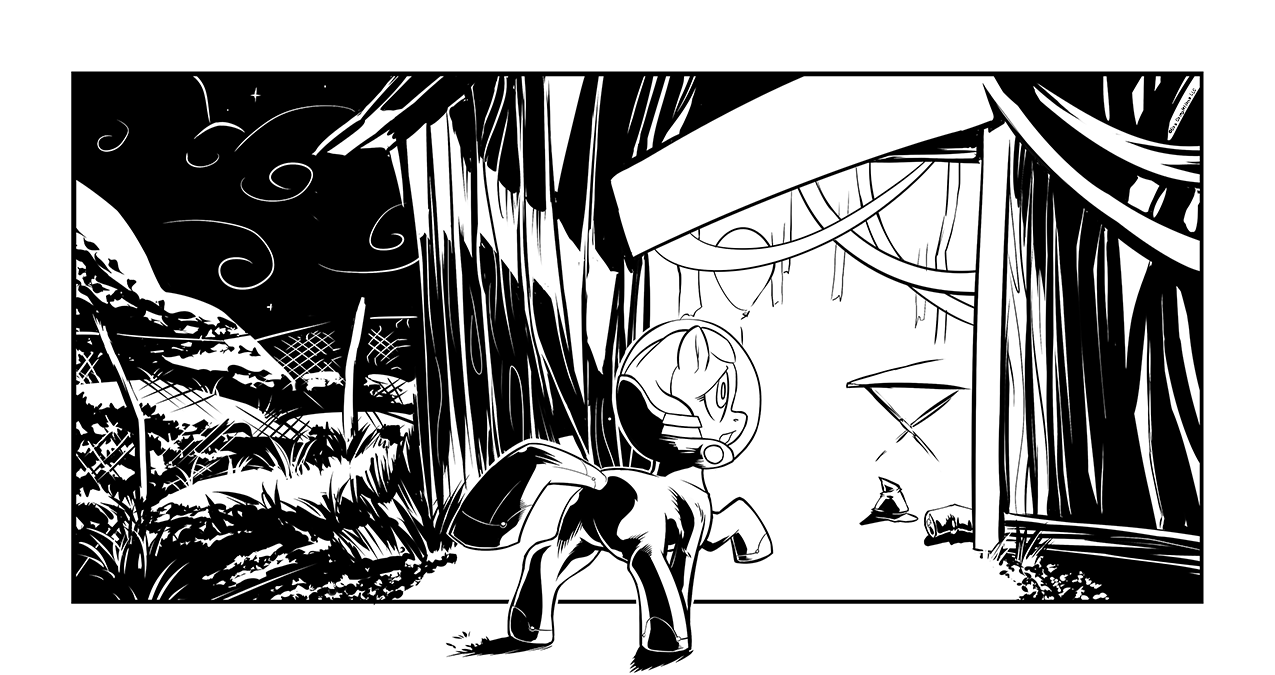
\includegraphics[width=0.9\linewidth]{image02.png}

\begin{intro}
    不需要带上礼物,能来就足够了!
\end{intro}

\daytimeplace{2}{4:00 PM}{赤兔山脉,52号国道北口}{Redtrotters ridges, Big 52 N Branch}

通常来说,穿着一套全封闭式环境适应服一点都不符合小马国时尚审美,但是大家也必须承认它还是能带来很多便利。首先如果你能从一次野火炸弹\footnote{野火炸弹(Balefire Spell):\emph{FoE} 设定之中的几个超聚魔法之一,类似于原子弹}袭击中幸存下来的话,你估计能够享受到渴死在环境服之中的待遇。其次它完全防水,并且基本上隔热,所以你也用不着雨伞或者墨镜。对了还有一点,它是柠檬黄色,所以基本上任何时候你都能被一眼看到。除非……大概……如果……你不小心埋在一大堆柠檬之中的话……那时你肯定不想被任何马看见,对吧?不过,很显然的是在废土上有时候隐匿行踪才是美德。

前提是帕比认识「时尚」这个词的话!

\horizonline

「嗨!我是快乐帕比!」穿着黄色的幼驹对着面前的俩小马微笑着。他们穿着和那天晚上那仨差不多。不过外表少了一些狂野,而且装备更精良。一只独角兽雌驹拿着一把防暴霰弹枪,搜寻着帕比后方是否有什么异常,另一只陆马身边似乎捆着一根大号长矛。要是帕比知道那是什么东西,这两匹雌驹的举动肯定会让她胆怯。

独角兽先开了口:「小鬼,你在赤兔的地盘上干什么?」

「那奇怪的衣服又是什么玩意儿?」陆马接着问。

「我在找我妈妈!」帕比兴奋地回答,伸出蹄子指着路的大概方向。「她在那边!」

俩部族小马相互对视了一眼,然后独角兽又问:「好吧,你妈妈叫什么名字,她是赤兔的?」

「啥是赤兔?」

独角兽的表情开始不耐烦了,不过陆马替她回答了问题。「我们就是赤兔。在52国道上从这里到盐块城都是我们的地盘,所以你想要通过这里,那么你就要通过我们的地盘,所以你妈叫什么?」

「我妈妈叫阴雨·黛丝(Rainy Days)!她超级酷而且总是给我唱歌,还会做很多好吃的!她是最棒的小马!等长大了我也要变成她那样!」

「好了,好了,我知道了。」独角兽不爽地打断她。「抱歉小鬼,但是我不认得什么阴雨,她肯定不是赤兔,你是独自一马吗?谁送你到这儿来的?」

「我有声音先生陪着我!」

「声音先生?」独角兽再次警惕地巡视着道路。

「是啊!他住在我的太空服里,有时候我们一起唱歌,但有时他的脾气也很暴躁,但没关系,因为他会帮我找到妈妈!」

「好吧。」雌驹松懈了警惕。「这样,我很抱歉,但如果你和你的隐形朋友想要通过这里,就得交路费。」

「啊……好滴?我有……」帕比开始在她衣服上的口袋上翻找起来,一路上她收集了不少好东西,大多是一些坏掉的玩具,还有她觉得有趣的东西。或许她可以分一些给这些小马。毕竟我们要彼此体谅,彼此分享\footnote{彼此分享,彼此体谅(You gotta care, you gotta share):这是S01E21中萍琪派的歌词},不是么?

「那么这个怎么样?」

不能用牙齿拿东西是一个很大的问题。她不得不改用她的蹄子,但笨重的橡胶靴使这项任务变得更加艰巨,而且她必须以十分尴尬的角度弯曲她的腿以便伸入她的鞍包。

「等等,我马上就能……呃……」

「{\mt 提示:该防护衣提供简单的操作魔法,可以通过HUD菜单来访问您的物品栏选择物品。}」

「啥?」

陆马看着帕比嘟哝着从她的鞍包中捣鼓出各种无用的垃圾。这个小家伙肯定没有什么值钱的东西。拿长矛的小马看着她的朋友使了个眼色。她若有所思地叹了口气,在对残酷的命运之神进行了短暂地内心祈祷之后,将长矛插入了小马驹的脖子上。快乐帕比忙着听她那衣服发出的各种抱怨。她像一堆砖头一样倒在地上,陆马将她放倒后,默默地咒骂着废土。

「你这是帮了她。如果没有她母亲,她连一天都活不下去,而且我们也不能把她带进来。这样总比让她被蝎尾狮吃掉好,或者比那更惨。你知道这里的小马驹会发生什么。」独角兽叹了个口气。

陆马注意到了独角兽的复杂表情,她补充道:「是啊,可怜的瑞吉……」

长毛马从尸体上拔出武器。当她退后一步时,粉红色的烟雾开始从衣服上的洞中逸出。雌驹注视着这个现象,疑惑不解。「嘿,瘦子,那是什么?」

独角兽用蹄子抓了抓头,「你肯定戳坏了防护服的某个魔法晶片……这东西可能有毒,我们站远点。」

「我们总不能把尸体留在这儿吧,感觉不太好。」陆马犹豫着,但还是躲开了粉烟。

「在你弄出那么多烟火之后,我可不打算靠近她!红蟑螂会解决她的。我们走吧,继续巡逻。」

俩小马最后看了倒在地上的小幼驹一眼,小跑着走开了,离开大路,然后爬过一个低矮的山脊,消失了。时间从路中间黄色幼驹的身体中流过。一阵冷风刮来,在光秃秃的树上沙沙作响。尽管有风,围绕着她的粉红色的云烟似乎也没有消散。

\horizonline

\daytimeplace{2}{4:30 PM}{赤兔山脉,52号国道北口}{Redtrotters ridges, Big 52 N Branch}

在一阵咯咯声之中,防护服发出的声音表示这个故事还能继续讲下去。

「{\mt 初始化系统。检查版本。警告,版本号匹配错误。启用安全模式。版本 0.2。检查装备状态。所有系统上线。检查到大型破损。激活修复魔法。恢复上次会话。读取目标001的个性化信息:快乐帕比,目标已死亡,体征稳定,检测完毕。}」

帕比的双眸在头盔里面眨了眨,就好像她刚刚睡醒了一场长觉。小幼驹打着哈欠,一滴粉色的口水从嘴角落在玻璃面罩上,但是立刻就被玻璃吸收了。

「唔唔……再睡五分钟,妈妈……」幼驹打了个滚,依然被那慢慢消散的粉云包围着。

「{\mt 破损修复,目标已经与危险环境隔离。}」

小雌驹睡眼惺忪地看着四周,先是皱着眉头,然后她似乎想起来什么。「哦,对了,妈妈不在,我刚刚怎么睡着了?」帕比想抓抓头但是蹄子被头盔挡住了。所以她眉头皱得更深了,非常不开心地耸了耸肩,并且若有所思地抱着头盔。

「{\mt 读取临时记忆,提示:失去信号之前最后一个行动,商谈买路钱。}」

「商谈啥?」

「{\mt 与赤兔商谈经过领土的通行费用。}」

% NOTE: 漏译

又来了。「鱼翅……啥?」

「{\mt 和漂漂小马聊天。}」

终于,小幼驹听懂了!「哦,对哦,漂漂小马!我想起来了!啊……他们哪去了?」

「{\mt 赤兔位置未知。将寻找该目标增加到任务清单中。}」

帕比一脸为难的抬起眉毛。「你们还要列个清单?从什么时候开始?」

「{\mt 清单在23小时之前创建。清单上项目:4项}」

「哇哦,我们还真有不少事1、2……呃……4是个好大的数啊,是吧?清单上有什么?」

「{\mt 主要目标:到达MoM。次要目标:解决防护服问题。次要目标:确认马尾伯爵或者至少回避他。次要目标:寻找赤兔。}」

在听完这个清单之后,一脸沉思表情的黄色幼驹戳着自己的头盔。「动动脑子,动动脑子……马芬!不……等等……不是那个……」几分钟之后,幼驹点了点头,双眸闪着光,「哦哦哦!放点音乐……啊……那个话挺多的小马台。」帕比一边听着广播,一边跟着箭头继续她的旅程。

52国道附近的荒地全都是小山和石头,这个地形的视野非常糟糕。这通常会带来很多不便,不过帕比一点都不在乎。

「嘿,声音先生,你刚才说什么关于口袋里面拿东西的事情?」

「{\mt 肯定。这个衣服装备了基础的操作魔法。}」

「呃……怎么用?」

「{\mt 读取说明。选择为幼驹和小呆准备的简单版。说出你要的物品名字,符合描述的物品会悬浮到你面前。}」

「啊……马芬!」一盒200多年前的马芬浮到了帕比面前,她咯咯的笑着,这东西在天上飘着的样子看起来傻乎乎的。

「嘿嘿,好好玩!黎明沙士!」一瓶黎明沙士代替了马芬。「玩具车!」这次一个看起来坏得很厉害的玩具车浮在了幼驹面前。「嘿嘿!我们应该多找点东西,我喜欢这个猜谜游戏!」

「{\mt 否定。这不是猜谜游戏,这是物品管理系统。}」

帕比拿起一块石头放进口袋里面。「石头!」石头立刻浮在了她面前。「耶!真灵!」当石头放回去的时候,石头的名字变成了「命运之石(The Rock Of Destiny)」,但是帕比基本不识字,所以她也没注意。

幼驹一边继续顺着路走着。一边不停地要着物品栏中的东西,其实并没有多少,总共她也只有四件东西,但是她有个大计划。

「哦,我们需要更多音乐!」

\begin{music}
千里之外那指路之星闪耀天穹

\begin{englishlyric}
    I can see that lone star from a thousand miles away
\end{englishlyric}

\medskip

指引迷失的我踏上家乡的归途。

\begin{englishlyric}
    Calling me back home, though I ventured far astray.
\end{englishlyric}

\medskip

当我向着那个灯塔勇往直前,

\begin{englishlyric}
    When I see that beacon shining for me all alone,
\end{englishlyric}

\medskip

它带我飞翔带我回到家乡回到小马国!

\begin{englishlyric}
    It calls me back to `Questria and my home!
\end{englishlyric}
\end{music}

\horizonline

\daytimeplace{2}{7:00 PM}{赤兔山脉,52号国道北口}{Redtrotters ridges, Big 52 N Branch}

这里的居民点看起来比棚户区稍微强那么一点点,至少没有拿臭水沟当护城河什么的。它的城墙看起来更像是一辆撞毁在民宅上的旧汽车,而不是什么防御设施。

帕比完全没有在意这些,一路蹦跶进城里,摇头晃脑地唱着电台里面的歌曲,一直到她面前地面上暴起一团尘土。

「嘿!你,我说了,给老子站住!」

帕比回头看着「城墙」,大概50多米远的地方有个小马举着一个大枪对着她。于是幼驹坐下来挥着蹄子微笑着。「嗨!我是快乐帕比!」

在那堆破烂后面举着大号来复枪的小马显然没有被她的热情感染到,板着脸说:「好吧,拿下那个大金鱼缸,我要看看你的脸!」

「呃……我真的很想这么做,但是我卡在里面了!」帕比想了想说:「实际上,这件事还在我的清单上!」

「好吧,你行……呆在那里把蹄子和武器都放在我能看得见的地方!」

「我不觉得我有什么武器……我有一块石头,算么?我可以丢它!」她蹦跶着说。

卫兵无奈的以蹄覆面,「喂,大号你去搜她身,你,黄色的小个子,给我乖乖站好!」

「好的,好滴,好得!」帕比笑着,不过她的回答显然让那路障后面的小马不满意。

「回答『是』就行了,只要别耍花招,要想大家都没事,就呆着别乱动,让大号做好他的活。」

棕色的大个子雄性独角兽走到帕比身边,看着幼驹在头盔后面的那张笑脸,她双眸之中的光亮现在小得几乎看不到,完全被头盔上各种HUD的光掩盖了。

「我擦,你穿的这身防辐射服保养得可真好……从没见过这样的……」

「当然!它超黄超聪明的,还可以变戏法!你看!嗯……马芬!」刚刚的那个马芬盒子立刻飘到帕比面前。

「哇哦,内置物品管理系统和次级操作魔法,这东西绝对贵得要死,你从哪儿弄到的?」

「中心城的一个漂漂小马给我的!」

「这么说……你来自中心城?」大号听起来不太相信她说的。

幼驹自豪的点了点头。「没错!」

「就是52号国道能看到的那座大山上的城堡么?」

「就是那儿!」帕比笑着回答。

「哦,怪不得你穿着全封闭防辐射服……好吧,我们别闲扯了……给我看你的通行证。」

帕比茫然的看着棕色独角兽,「我的啥?」

「你没通行证?你来的路上没碰到巡逻么?」

「我看到俩小马,一个像我一样的陆马,还有一个是……犄角……单角……哦哦……独角兽!他们超和善超漂漂!」

「没错,没错……好瘦子和冰苏打」大号打断了她后面的话。「他们没和你提什么买路钱之类的?」

「呃……不太记得了。我们聊了一会,然后我有点犯困他们就丢下我走了。」

「随便从她身上拿点什么然后给她个通行证!」

「呃……好吧……」

那小马搜了搜帕比身上,但是除了石头和衣服没啥东西,他甚至想解开那外套,但是不管他怎么弄看起来都没什么用。「好吧,很抱歉小鬼,我也是迫不得已……」他们给了帕比一个中间染了红色的破锡罐。「给你,给幼驹的特别折扣。」

「我会告诉我妈妈你们对我很好,谢谢你们漂漂小马!」

「就这样吧……说起来,一个幼驹穿着防辐射服自己在52号国道溜达?这里可不是什么好地方……」

「我去找妈妈!」帕比看了看附近似乎想要找个标志物,然后指着东南方说:「就是那边,好了我走了拜拜!」幼驹不等他们回答就走掉了。

「但是在哪个方向的就只有嘉年华……啊等一下小鬼!那里很危险,别去那里!」大号举起蹄子,但是转念一想,她和他非亲非故,在废土这种地方多一事不如少一事。

黄色的小雌驹继续顺着小路往前走,她看到那条弯弯曲曲的小路上有一些马为的痕迹,不知道谁在路里埋了很多削尖木棍。帕比在小路上闻了闻,然后就再没管它,在石头上爬上爬下,跳来跳去的游戏对于一个这么大的小幼驹来说是超有趣的。随着夜色慢慢变深,幼驹也渐渐走进废土深处。

\horizonline

\daytimeplace{2}{10:30 PM}{嘉年华,废土}{The Carnival, Wasteland}

一个巨大的谷仓坐落在小小山谷之中,从上面斑驳褪色的痕迹可以看得出它曾经漆成粉色。它被环绕山脊的栅栏包围着,栅栏上每隔一段就有一个自动炮台。这幢建筑和栅栏还有炮台都已经破旧不堪,但是那些炮台依然颤颤巍巍地来回转动着保卫这里。

「{\mt 警告,侦测到自动防御炮台,敌对模式。威胁等级:中等。}」

敌对这个单词让帕比立刻警觉起来,她站定了看了看四周,「那伯爵又来了?在在哪?那马还真纠缠不休,呃,我觉得还是小心驶得万年船。」小小马连忙躲在一个石头后面,警惕地看着那个马尾伯爵先生是不是追来了。「关了音乐,声音先生,我们在躲猫猫呢!」她屏住呼吸竖起耳朵听着周围。

「{\mt 开始和防御系统建立通讯连接。交换协议。申请进入。申请成功。路障已清除,请继续前进。}」

「我说安静!附近肯定有小马……或许是那伯爵,我们应该超级小心!」帕比从掩体后面探出头来,回头看着附近以免有什么可怕的东西就在她身后,然后她慢慢走过栅栏,炮塔马上指向她的方向,但是它们在罗盘上的红点从红色变成了粉色,炮塔又回到了它们通常的防御方向。

「嘿,声音先生……我叫你别放音乐了……」

「{\mt 肯定。无线电已静默。}」

「那么为啥我还能听见音乐?」

「{\mt 声源检测。音乐来自MoM建筑物。}」

「里面?妈妈在谷仓里面?还有音乐和其它东西?妈妈在开派对?耶!」帕比立刻停止了躲藏,四蹄并用从山坡上直奔谷仓大门,最后幼驹猛地踢开大门跳了进去。

「惊喜!」

谷仓里面的空间非常大,而且很开阔,还有两个阁台,一个在门上方,另一个在对面。地面整理得很平,并且铺了一层稻草,墙壁上挂满了破旧的彩带和花环。屋顶上吊着几个看起来很惨的糖罐,还有一大堆灯泡、没气的气球还有其它破烂不堪的旧东西。几盏勉强能发出光亮的旧挂灯无精打采地照亮着这里,唯一看起来能正常工作的就是那个凑合能发出点儿声音的破旧喇叭。

在屋子的正中间有一个派对长桌,桌边已经有一些客人了——一袋面粉,一堆石头,一个装了不知道已经烂掉的什么东西的锈桶,它们都带着一个派对帽\footnote{此处可参考正剧《独马派对》}。哦,座位上还有很多骷髅,至少一打了无生机的小马坐在桌子边,头上带着派对帽,空旷的眼洞看着面前空空如也的盘子,甚至有几个看起来像是干掉的木乃伊而不是骷髅。实际上,其中之一看起来像个饿到皮包骨的小马,而远处的角落堆着一大堆白骨。

「{\mt 警告,侦测到轻微辐射。警告,空气中检测到毒气。分析中,毒气成分:一氧化二氮\footnote{一氧化二氮:无色有甜味气体,又称笑气}。威胁等级:微不足道。}」

「哦,看呐,新客人!」一个看起来像是派对主持的影子从座位上站了起来。那是一只金属的小马,发出旧唱片一样的吱吱声。在昏暗的灯光下,她看起来就像是一只长着粉色鬃毛的粉色小马,但是靠近之后,帕比发现到她是靠轮子移动的,就好像她蹄子下面穿了电动滑冰鞋一样!「看看你的样子!我想你是来这里参加化妆舞会的,不过我很抱歉通知你舞会已经取消了!但是你可以继续穿着你的外套!因为超酷!」另外一件奇怪的事情是,一般小马说话的时候嘴巴会动,但是这个小马印在脸上的微笑却完全不会动,取而代之的是她在说话的时候眼睛却会诡异地闪闪发光。

「呃……你是个……机器马?」帕比迟疑着问,因为她想起来妈妈告诉她如果其他小马看起来很奇怪不要随便当众说出来。

「那是,当然!你真是个聪明的小马!我是娱乐用机器萍琪 MK II 原型 03 号,这是我的生日派对!想要加入么!我可以给你腾出位置,你知道的,有些客人有些不开心,坐在那里不说话。」

「呃……我是快乐帕比……我……呃……我找我妈妈……她应该在这边……大概?」

「太棒了!等她来之后她可以一起加入我们!现在坐下来,你想要吃点蛋糕么?」

帕比没有参加派对的兴致,她应该能在这里找到自己的妈妈,而不是这个破烂生日派对……或许和这个机器马一起玩一会之后她可以帮她。所以幼驹坐在位置上之后看着其他客人。

诡异这个词已经不能形容现在帕比的情况了。那些骷髅正在看着她,所有那些死掉的东西还打扮得像派对来宾一样,尤其是那俩超级瘦的木乃伊……

等等!一个木乃伊居然转过头来了?「求你……哈哈哈……别让我……哈哈哈……笑了……」她还说话了!

这个小木乃伊是一只有着浅黄色毛皮和橘色鬃毛的独角兽,她看起来病得很厉害,幼驹笑个不停但是看起来却一点都不开心,似乎她只是止不住要笑。她眼睛很空洞,而且鼻血流个不停,鲜红的鼻血流得她浑身都是。「求……呵呵……让我回家……」她喃喃地说着这些话,似乎她已经说了上千次,可她仍然在不停地说着,好像说够了次数之后就能从这个噩梦醒来一样。

帕比感觉背后一阵恶寒,好像后背滑过一块冰块似的。这地方不对劲,她想走。但是妈妈在这里,她可能……可能是……那堆……骷髅的……其中之一。

惊恐万状的帕比几乎不能自已。这简直就是那个原本超级和善的机器马觉得烦了,于是就开始伤害小马的故事翻版!已经有太多的小马死在这个毛骨悚然的嘉年华派对上,而马上还会有更多牺牲品!而且她妈妈可能还在邀请名单上,如果她……不对如果她已经……等等!那机器马似乎说了什么她不在这里的话?但是那个机器马可能在说谎。她会说谎么?谁还管这个!这个粉色的东西绝对是个大坏蛋,帕比不想再和她玩了!

那一瞬间,帕比的视线和那个坐在桌边咯咯笑的小幼驹相交,那小马也想她自己的母亲,这里是个坏地方!「快跑,快回家!」帕比看着她,一直到小独角兽离开座位。机器萍琪走过去打算拦住她,但是帕比正要找它算账。

「我妈妈在哪里?」她从座位站起来问。

「等派对结束我们可以一起去找你妈妈,好吗?要不要来点儿黎明沙士呀?」

小独角兽趁机一步一捱地挪向门口。

「抱歉,派对还没结束,你不能走!」

「我妈妈在哪里?」帕比走向那个粉色的马形机械,吸引她的注意。

「好了,好了,乖乖的,别坏了派对兴致。你想玩钉马尾游戏么?」

粉色的火花在帕比双眸中燃烧。「我妈妈在哪里?你把她怎么了?」

「错误。物件妈妈未找到。拜托,别生气。我觉得你妈妈很快就会来接你的!」小独角兽回头看了一眼,靠着大门勉强让自己站好,她颤颤巍巍地走着就像一个乌龟一样。机器萍琪滚着轮子走向她。「站住别动!长辈没允许,不准离开!」

「不要忽视我!她应该在这里的!讨厌的机器马!我不会让你再伤害别的小马,不会让你伤害我妈妈!」帕比低头弓起身子,「石头!」她低声咆哮着。

「请不要说脏字,开始镇压行动,目标免疫毒气,需要使用物理力量,建议使……」

咣当!

「我!」帕比双眸明亮地闪烁着,头盔上反射着粉色的火光,黄色的幼驹直接跳在机器马脸上,不停地用「命运之石」用力砸她。

「妈妈!」帕比咆哮着用双蹄抓着机器马的脖子,拿出自己吃奶的力气和它头碰头,力气大到头盔上都撞出了蜘蛛网一般的裂痕,同时也撞坏了机器萍琪的脸部面板,露出了后面的电路和机械组件。

「在!」帕比一只蹄子继续抓着机器马的脖子,另一只蹄子不停地砸着漏出来的电线,每一下都会让机器马脸上飞出一些被打烂的电路和零件,直到她砸到一个魔法晶片。紧接着机器马就像身体里塞满了粉色和黄色烟花一般炸开了,把帕比炸飞到房间另一头。

「哪里?」被炸飞的帕比一屁股坐在了一座自动炮台上,这东西在她打烂了那机器萍琪之后就冒了出来,电子的爆裂声就像是在悲鸣,那炮台顿时爆成了一团火花,剩下的炮塔则锁定了帕比射出无数五颜六色的激光弹幕,不过那些光线完全无法射穿帕比的防护服。

「别闹了!告诉我,我妈妈去哪了?」帕比径直冲向其中一个炮台,用力撞向它,撞得它歪向一边,而那炮塔还在疯狂的射击着,所有弹幕都打在了天花板上,对于破旧的木质建筑而言,激光的破坏力可比对一件涂有反射材料的防护服有效得多,帕比转身一蹄子把它从底座上踢飞了下来。虽然那机器闭嘴了,但是天花板同时也裂开了。

「妈妈!妈妈你去哪了?妈……妈!」完全不管正倒塌在她周围的谷仓,幼驹疯狂地跑向角落的骨头堆。「声音先生,你看见我妈妈了么?她在哪里?」

「{\mt 错误,地点已到达,斗志部分部已经找到。}」

「你又说什么乱七八糟的?我要妈妈!你说她在这里!」

随着最后一声低沉的隆隆声,历史久远的谷仓终于整个垮下来砸在了帕比的小脑袋上。

黎明的第一道光芒照亮了废土之上永远不散去的云层,一个娇小憔悴的独角兽小雌驹从前MoM建筑倒塌的烟尘之中爬出来。炮台静静地躺在哪里,因为已经失去了动力源,就连音乐声也消失了,持续了200年之久的挽歌终于结束。只有几丝火星在废墟之下闷烧着,吞噬着那些残存的朽木。

\horizonline

\daytimeplace{3}{9:15 AM}{嘉年华,废土}{The Carnival, Wasteland}

即使到现在,这个被诅咒的地方依然没有找回安宁。

「我没有让你找这个可怕派对地点,我让你找我妈妈!」废墟下面闷声说。

「{\mt 否定,你说了……}」外套播放了帕比之前说话的录音。「声音先生……妈妈在哪儿?」

「我就是这么说的!」

「{\mt 肯定。斗志部最近的可用分部已经定位并且标示在地图纸上,并且在几小时前已经被设定为主要任务目标。现在它已被摧毁。}」

「不用你说,它爆炸了两次。」

「{\mt 否定。它不可能爆炸两次。主要损害已修复,系统运转正常等待下一步指令。}」

帕比静了静,整理了一下思路。对声音先生凶也没有用,主要是因为没什么东西可以揍,所以她应该聪明点,她是个聪明孩子,对吧!反正那个机器萍琪是这么说的!

「好的好滴好得……覆水难收……或者说,坏谷仓没法修……既然你说妈妈不在这里,那么然后去哪里?」

「{\mt 警告,尽管已经解释完毕,但现在依然有一个重大误……}」

「喂,闭嘴啦!下一个妈妈可能会在的地方是哪里?」声音先生该不会是因为一直干活不能玩,所以闹脾气了吧……笨衣服……

声音沉默了一会,如果他有更复杂的智能的话,他可能会说些别的,或者至少觉得沮丧,但是这个程序就只是为了服从命令,他只能做到这一点。

「{\mt 下一个MoM地点定为主要目标,位置已经显示在罗盘上。}」

在帕比终于把自己从废墟里面挖出来的时候,一个新的粉色箭头出现在罗盘之上。幼驹跳下碎石堆,抖了抖身上的尘土然后说。

「看到了吧,如果你合作的话什么事都这么简单。」

「{\mt 肯定,合作是魔法。}」

一个金属的笑声打断了这场对话让帕比抬起了头,她看到几天前见过的那个嗡嗡响的机器精灵。

「哦,是你啊提问者,嗨!」幼驹微笑着。

「是守望者……不管怎么说这都太无厘头了吧?」

「什么?你说这个派对?你信我的,你啥也没错过,这是最烂的派对,没有之一,所有小马都无聊到死,呃,真的死掉了。」

「那么,找到你妈妈了么?」

「完全没有。」帕比微微皱了皱眉头,然后又笑了起来。「但是我们还有很多地方要看看,所以没问题!她肯定在哪里,对吧?」

「呃……大概……吧?」机器顿了好长一会儿,「顺便,我可以问问你打算去哪么?」

「那边!」小雌驹用蹄子指着,然后补充道,「这次我觉得会走运!」

「所以,你打算检查下一个『MoM』地点?」

「当然!」

机器又一次顿了很久,「你还觉得下次会走运?」

「没错!」

「好吧,的确是,反正已经……很好,帕比,我该走了,祝你旅途愉快。」

「当然,提问者先生!祝你一路顺风!」机器精灵转头飘走了,还大声广播着贪食精灵进行曲。

「哦,对了!声音先生,来点音乐吧!」

\begin{music}
我不想把整个小马国点燃,

\begin{englishlyric}
    I don't want to set Equestria on fire,
\end{englishlyric}

\medskip

我只想点燃你心中的激情!

\begin{englishlyric}
    I just want to start a flame in your heart!
\end{englishlyric}
\end{music}

\horizonline

\daytimeplace{3}{2:00 PM}{赤兔平原,52号国道北口}{Redtrotters Flats, Big 52 N Branch}

帕比回到了52国道。把那些山丘抛在脑后之后,眼前出现的是一望无际的大平原。远处大城市摩天大楼的剪影面前,点缀着近处一些旧农舍的残骸。在路边有很多旧的马车,有一些是轻巧的小车,有一些是载货的大车。它们都面临着同样的命运——独自在路上锈烂。

「嘿!说你呢,等等!」帕比转向叫她的声音来的方向。

黄色的小雌驹看到过来的是昨天那俩母马,她微笑着挥舞着蹄子,她们其中之一在30米开外停了下来,并举起一把突击步枪,另一个慢慢靠近,并且谨慎地举着动力长矛。

「好的,我的神奇小丫头,乖乖站好大家都不会受伤。」

「呃……我们在玩游戏么?」

独角兽继续用枪瞄准着帕比,另一个小马回答道。

「没错,差不多,想要玩么?」

「好棒!我可以先来么?可以么?可以么?可以么?」帕比已经开始和她这个年纪孩子一样兴奋的上蹿下跳了。

「当然,我们玩我问你答游戏,你如果答不上来你就输了!懂么?」

「耶!猜谜游戏!我超喜欢猜谜游戏!问我,问我什么都行!」

「好,第一问:为什么你嗓子眼被动力长矛戳过之后还活着?」

「啥和啥?」这个问题太难了,帕比完全不知道什么是动力长矛,听起来似乎是吞下什么东西并且不被噎到的意思。「呃……可以略过这个问题么?」

俩母马交换了一个眼神。「或许,这家伙只是个笨小孩?」陆马提议道,独角兽叹了口气,「好吧,我们问问别的事情。」

「好吧,小鬼,那么……为什么你去嘉年华?」

「你是说那个旧农场?好吧,这个傻蛋声音先生告诉我妈妈在那里,你猜结果怎么回事?她没在那里,而且那里还有个全世界最无聊的派对,那个发疯的粉色机器马还想伤害我妈妈,我很生气,但是机器马爆炸了,然后有个怪东西开始往我身上照讨厌的光线,剩下的我记不太清了,只记得整个农舍都砸我头上了,最近真是被房子砸了好几次……」帕比想了一会,又补充道。「我希望那个瘦瘦的孩子能安全回家。」

「瑞吉还活着,所以我朋友还没开枪打你。」陆马深吸了一口气。「所以你复活了以后走了这么远跑到嘉年华,然后把那个天杀的地方毁了,并且救了瘦子的妹妹,这一切只是个意外?」

「我……我不记得我做了那些事情,不过既然你这么说……」

「然后你一直只是在找你妈妈?」雌驹抬起眉毛,疑惑地问道。

「是的,你知道她在哪?」

「没错,她就只是个笨小孩。」陆马无奈地以蹄覆面,而独角兽在她身后大笑着。

笑过之后,独角兽表情变得严肃起来。「不管怎么说她救了我血亲,我欠她的。」

「那么你想怎么办,瘦子。」陆马问。

「我不知道。」瘦子放下枪口靠近那个冲她微笑的快乐帕比。那天真无邪的小小微笑融化了这个铁血女独角兽的铁石心肠,她将一只蹄子放在帕比头盔上。

「我不知道你是好是坏,不过我欠你一次……所以,谢谢。」瘦子递给她一个金属片,上面刻着一颗吃了一半的白色苹果,「拿着这个,这是通行证,如果你去盐块城,把这个给卫兵看他就会让你进去,懂吗?」

帕比睁大眼睛看着她收到的馈赠。「哇哦,谢谢!礼物,我超喜欢礼物!漂亮的大姐姐非常感谢你!」

独角兽继续说:「你终结了我们一族的噩梦,还救回了我唯一挚爱的血亲,我希望你能找到你所寻找之物,小小幽灵。」

「哦哦哦,你也有这么可爱的时候?」陆马低声揶揄着。

「给我闭嘴,赶紧走,苏打,我们还在巡逻呢!」

「嘿,你哭了,瘦子?」

「你闭嘴好么,绝对不准和其他马提起这件事!」

「好吧,说起来,现在我对之前杀过她有些愧疚了。」

两只小马向着粉色箭头相反的方向走开了,帕比挥着蹄子目送他们消失在山脊之后。

「我喜欢漂漂小马,她们真漂亮!」帕比笑着,然后出发走向大城市。

「嘿,声音先生,我可以问你一些事情么?」

「{\mt 肯定,请陈述您的请求。}」

「等我们找到我妈妈之后,你会离开么?我是说……我不想让你走。」

「{\mt 否定,在幼角药剂的影响下,该装备已经永久与您融合。}」

「呃……这就是说,我们能永远在一起?我找到妈妈以后还能和你在一起?」

「{\mt 肯定。}」

帕比微笑着,和往常一样只听她想要听的事情。

「好的声音先生,你已经知道我们现在该干啥了吧。」

「{\mt 肯定,基于数据分析,对您的日常需求预测现在有95\%的准确率。}」

广播开始播放声音,帕比一边唱一边走下去。

\begin{music}
你和我,在一起,

\begin{englishlyric}
    You and me together will be,
\end{englishlyric}

\medskip

在一起,在一起,

\begin{englishlyric}
    Forever you'll see,
\end{englishlyric}

\medskip

我们是,好姊妹,

% NOTE: 兄弟 -> 姊妹

\begin{englishlyric}
    We two can be good company,
\end{englishlyric}

\medskip

好姊妹,好姊妹

\begin{englishlyric}
    You and me
\end{englishlyric}

\medskip

你和我,好姊妹……

\begin{englishlyric}
    Yes together we two\dots
\end{englishlyric}
\end{music}

~\vfill

\begin{note}
升级。我想我们早讨论过这个问题了吧。

否定。升级是辐射小马国同人的既定内容。

好吧好吧,真烦,我可以理解帕比的心情了,那么这样。

增加任务专长:升级是命令——现在你可以正常升级了,耶!
\end{note}






\chapter{迷路羊群}

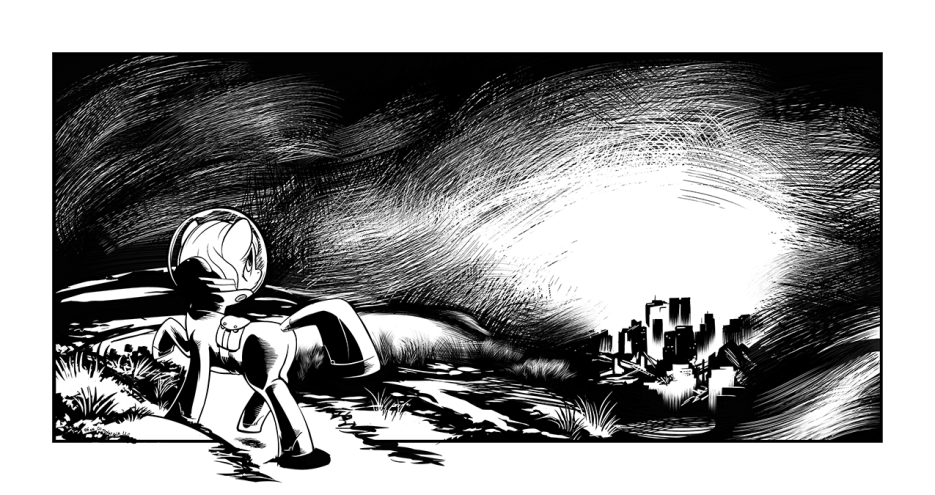
\includegraphics[width=0.9\linewidth]{image03.png}

\begin{intro}
很久很久以前,在逐渐消亡的小马国土地上
\end{intro}

「{\rt 女士们,先生们,晚上好!这里是孤狼\footnote{孤狼(Lonesome Pony):后面缩写为 L.P.}的52电台!虽然,野马 DJ PON-3 尥蹶子踹好了吠城(Fillydephia)的广播晶片,所以十马塔(Tenpony Tower)的广播在整个废土都收得到!但是只有在这里才有你想要听到的所有52国道新闻!}」

然后一阵悠扬的音乐持续了几秒钟。

「{\rt 以上就是大狗\footnote{大狗:这里指孤狼}能提供的全部服务了,现在回到本地新闻。嘿,小马们,你们害怕幽灵吗?也许你们应该害怕。你们记得嘉年华的故事吗?如果没听过不要紧,老朋友L.P.现在就给那些没预习功课的小马们补补课!}」

「{\rt 在52号国道最最最最最北边的地方,有一处大家不知道的农舍,赤兔们叫它嘉年华。那是一个年代久远的遗迹,但是不像它的兄弟姐妹一样,嘉年华从未真正安眠。自从我祖母记事以来,每隔一年就会有一个幽灵从那里出现,游荡在附近的山丘,邀请大家参加她的聚会。当第二天早上来临的时候,就会有小幼驹神秘地消失,然后再也回不来了。感谢那些无处不在的激光炮台,靠近嘉年华几乎是自杀。不过如果你靠得够近,就能听到在那被诅咒的谷仓里面传出音乐声,就像是整天整夜地在狂欢一般。}」

「{\rt 我的小马们,看起来似乎是有谁大喊着『我不怕幽灵!』然后冲进那派对中把整幢农舍的房顶掀翻了。非常勇敢。现在赤兔的小幼驹终于可以安心睡觉了。我很好奇这个神秘的英雄是谁,但是大家都说她也是一个幽灵。是一只在粉云之中穿着黄色防辐射服死而复生的小幼驹。干得好,黄色幽灵。你给废土解决了一个大麻烦,你面前还有一百九十九个要解决!哦,我有提到今年嘉年华的被害者安全回家了吗?塞拉斯蒂娅公主祝福我们!现在还是继续我们的小马萨克斯吧!}」

\begin{music}
我在千里之外看到指路之星,

\begin{englishlyric}
    I can see that lone star from a thousand miles away,
\end{englishlyric}

\medskip

它在远处向我招手叫我回家。

\begin{englishlyric}
    Calling me back home, though I've ventured far away.
\end{englishlyric}

\medskip

指路之星如灯塔般给我带路,

\begin{englishlyric}
    When I see that beacon shining for me all along,
\end{englishlyric}

\medskip

让我回到小马国回到我的家!

\begin{englishlyric}
    It calls me to Equestria and a home!
\end{englishlyric}
\end{music}

\horizonline

\daytimeplace{4}{00:30 AM}{盐块平原,52号国道北口}{Salt Cube Flats, Big 52 N Branch}

帕比顺着52国道一路向南,远处大城市的剪影从地平线上跃升成为一个高楼林立的巨大水泥丛林。幼驹走了整整一天,而现在阳光消逝在黑暗之中。小雌驹眼睛中闪烁着的亮粉色光芒照亮了她的道路,虽然没有阳光,但还是可以清楚地看到盐块城那个微微发光的圆顶建筑,还有几座巍峨的摩天大厦耸立在一片漆黑的废墟之中。

差不多午夜的时候,小雌驹看到一个小车队从他的方向一起往南走,大概有半打小马和非常非常奇怪的……有两个脑袋的牛跟着他们?帕比惊奇地坐在地上,等待着他们靠近。显然车队卫兵也很快发现了幼驹,毕竟她是个坐在路当中的光源。当然,卫兵做好了战斗准备。

一个穿着轻型战斗鞍具的大块头低声问着旁边的小马。「你觉得……这个就是新闻中说的那个『幽灵』吗?」

卫兵的领头,一只带着大号左轮枪的陆马耸了耸肩,举起蹄子示意车队停下来。

「不清楚,但是我不冒险,所以我们慢慢来,你们俩去旁边,另外俩站在这里,我去交涉,好好掩护我,要不然你们别想领薪水。」

两个卫兵离开车队向旁边的小路前进,绕到帕比的侧翼,同时领头走出车队,两个卫兵保持距离守在后面。小雌驹的样子看起来很诡异,一个发出粉色光芒的大圆头盔安在一个小小的黄色轮廓上,不过的确是个很明显的靶子,卫兵领队一边小心靠近,一边祈祷她的卫兵在发生什么突发状况的时候能够救她一命。

「嗨!我是快乐帕比!」幼驹举起一只蹄子向领队挥舞着。好吧,至少她看起来还算友善。

不过在废土生存指南上,不止一次强调过「有备无患——看起来友善不等于安全。」

「好吧,站在那里别动,说个不让我把你变成一堆化肥的理由。」

帕比咯咯笑着,奇怪的话总能逗乐她。「喂喂,漂漂小马爱说笑!我不叫华菲!我是帕比,你叫什么名字?」

卫兵头头迟疑着,这个幼驹只是在冒傻气还是给她设了一个精心布置的圈套?但是经验告诉她有哪里不对劲。「对,我是固体虫。你独自旅行?」不等回答,她的卫兵已经开始检查附近了。

「当然不是,我和声音先生一起!他有时候超级聪明有时候超级笨蛋,取决于……不管怎么说他知道我妈妈在哪里啦!」

「那么……这个声音先生又在哪儿?」

「在这个太空服里!看到这些灯和漂亮点点了么?他能让这些东西出现!」

固体虫仔细看了看衣服的头盔,不去管帕比那俩闪闪发光的大眼睛,的确有一个HUD,和一些高级战斗鞍具用的瞄准设备差不多。一看到这个看起来价值连城的上古装备,她很想知道一个幼驹怎么能找到这种好货?但是那粉光总让她觉得不太自在。简单地说,固体虫干了很久护卫,见过废土上的不少东西。

「这么说,你应该是从中心城来的?」

「对哦!我家的房子就在……呃……正好在山脚下的四叶镇,不过有一天它塌了,所以现在我在找我妈妈。她不在声音先生说的一个旧农场,不过他说这个大城市还有另一个大地方。所以我要去那里看看!」帕比用蹄子指着南边说。

固体虫听的时候点了几次头,举起蹄子示意车队可以安全通过。在车队开始前进的时候她说。

「你可真能聊,不是么?孤狼刚讲到你在嘉年华的大冒险\footnote{大冒险:冒险(exploit)和后面的爆炸(explode)似音}。」

「我的啥?你说那个旧农场,我没炸了那里,农场自己爆炸了,小傻瓜。」帕比咯咯笑着。「那个机器萍琪绝对是个坏蛋!虽然开始很可怕,但我可是很勇敢的哦!」

固体虫挠了挠头,不想让帕比在闲扯下去了。「呃,没错,你很棒,我很想继续聊一会儿,但是我们还有事,如果你想去盐块城,那里的尸鬼集会在圆顶里面,我想他们把那里称作『炫彩』。别在城里闲逛,城里的人不喜欢你们。不管怎么说,祝你好运,小幽灵。」

当车队路过的时候,其他小马都好奇地看着帕比,但是固体虫和一个紫色红棕的独角兽说了两句,于是他们继续前进,黄色的幼驹很吃惊地看着那些双头牛,并且拼命地挥着蹄子,一直到他们消失在夜色中,然后她继续独行向南走。

\horizonline

\daytimeplace{4}{11:30 PM}{闹市区,盐块城}{Downtown, Salt Cube City}

这里的大门只是个用沙袋和破金属片堆成的壁垒。在一个木制平台上,有只穿着金属马铠的小马坐在一挺加特林机枪后面,另外两个门卫正在检查每一个想要进盐块城的小马。最后一个穿着军官制服的独角兽则坐在一个金属小房子里面写着什么。

虽然说现在快到正午了,但是城北门外和废土其它地方一样空无一马。这次帕比早有准备,她把那个有着白苹果的铁片给卫兵看。其中一个小马走过来,另外的几个卫兵则举起了武器。

「我看看。没错,就是这个通行证。那么,你叫什么名字,来做啥?」

「我叫快乐帕比!神秘的漂漂马你叫什么呢?」

卫兵抬起头盔的面罩,一脸不爽地看着帕比。「远见下士,好了,现在可以告诉我你来干啥了吧?」

「哦,这个问题我知道!我在找我妈妈!她大概在这个方向!」帕比伸出蹄子指向那堆残破不堪的建筑给卫兵看。

「好吧,够了,还有个问题,为啥你穿着全套环境防护服?」

「哦,这个么?我困在里面出不来了,不过没关系,因为有个狠好心帮助我的神秘声音也住在里面。」然后幼驹小声对远见咬耳朵。「不过他一点也不擅长找谁,不过别和他说,因为他脾气不好。」

卫兵放下面罩耸了耸肩。「只要你不打算在闹市区引爆超聚魔法,你想怎么穿就怎么穿。欢迎来到盐块城,小鬼头。」

幼驹连忙头也不回地跑过路障,但是远见在她身后喊着。「哦,对了,提醒你一下,别接近那个圆顶,因为那里面有野生尸鬼,而且有很多辐射污染。」

「好的好滴好吧!拜拜卫兵远见先生!」帕比跟着粉色箭头的方向,从那几个摩天大楼里穿了过去。

这里的闹市区和52号国道的其它街区差不多,有卫兵在往来巡逻,防止小马们在街上火拼。还有各个不同的贸易公司在街上竖起来的广告牌。比如『水农』或者『飞驰子弹』甚至还有一些雇佣兵和附近一些部落的交易代表。这个完全开放的市场看起来就是城市的中心,不过这个城市的真正中心是那四栋经过百年战争和风雨洗礼依然屹立不倒的摩天大楼。

盐块城在战争中曾经就被一个超聚魔法击中,不过运载超聚魔法的魔法导弹似乎出了一些问题,弹头击中了城市郊区的盐块圆顶,击穿了那个圆顶建筑的房顶,然后在里面爆炸了,坚固的圆顶保护城市免受冲击波的伤害,但是城市还是受到了放射性尘埃的影响。在之后的岁月中,城市里的大多数高楼大厦都在岁月的侵蚀下一个接一个地倒塌。但是那四座基本没有受损的摩天大楼依然在城市中心屹立不倒。

这四座高塔就是盐块城权力的象征:其中两座双子楼曾经是某个大型国际贸易公司的总部,而另一个和他们差不多高的大楼是一个强大的雇佣兵公司——聘蹄(Hired Hooves)的总部,最后一个,也是最小的一个,上面贴着白色苹果标志的大厦。住在里面的是这个城镇的所有者。整个城镇的所有交易都要向他们交税。白苹果同时也是聘蹄的主要兵员提供者,因为聘蹄的很多士兵都是这个家族的小马。

帕比站在一个染着红色印记的帐篷面前——这个印记表示帐篷的所有者是赤兔部落。这个商店的架子里面摆满了各式各样的铠甲和肉搏兵器,一个带着旧牛仔帽的雌驹坐在帐篷中间的一个弹药箱上。

「嘿,穿得不错的小家伙,你是不是从北边来的?」雌驹很富有魅力地笑了笑,用一只蹄子推起牛仔帽。牛仔帽下面露出了她前额上的独角。而在她臀部上的可爱标记看起来像一个棒球棒。

「嗨!我叫快乐帕比!」幼驹挥着蹄子走向雌驹。她指着帐篷外面的方向说:「我从那边来!」

「我叫强攻,我想你就是孤狼昨晚提到的那个家伙。」

「呃,你说那个在音乐频道唠唠叨叨的家伙?」帕比若有所思地挠着她的头盔,「上次我就听他说什么喝纯净水很重要。」

「不,不,我是说你是新闻里面说的那个『黄色幽灵』吧?或许附近不只有一个小马穿着防辐射服闲逛?不管怎么说,你想买点啥?」

帕比皱着眉头,「为啥大家都叫我幽灵?」

强攻笑出声来:「就是你嘛,我就知道!」独角兽轻抚着自己的下巴想了一会,「不管怎么说,作为一个拆了那诅咒农场的英雄,你是不是有点年轻?实际上你这个年龄就你自己在废土上冒险可不应该……你难道是个童子军\footnote{童子军(Crusader):可爱标记童子军的大名在废土上可谓如雷贯耳}?」

「当然不是,我是在找我妈妈!而且我不孤单呢,声音先生陪着我!」

「你妈妈?或许我可以帮你,毕竟我在闹市区认识很多小马,你妈妈叫什么名字?她可爱标记是什么?」

快乐帕比大概描述了一下。「哦,她名字叫阴雨·黛丝,她毛皮是紫色鬃毛是橙色,她的可爱标记是有着雨点的云彩!你见过她么?声音先生说她在这附近!在那边!」帕比指着那个半毁的圆顶说。

强攻摇了摇头。「抱歉,小鬼,完全不记得有这么一个可爱标记的小马,也不记得听过这个名字。」卖货的独角兽皱着眉头看着幼驹指着的方向,「你说那边?那可不是什么好地方,那里辐射很强,而且那里唯一一个比较完好的建筑物就是圆顶,听我的,你绝对不会想到圆顶附近的。」

「圆顶?那是啥?」

「那里到处都是野生尸鬼和其它可怕的东西,虽然说你穿着防辐射服不怕那里的辐射,不过最主要的问题还是那里的居民——一小撮鬼迷心窍的尸鬼。他们基本上就是个会行走的定时炸弹。虽然他们看起来暂时很文明,不过不知道什么时候他们就会发疯攻击小马。而且现在白苹果也正在想办法除掉这些快腐烂的脑袋——他们会打爆每个走出废墟的尸鬼头。但是他们没办法进去检查,如果你不免疫辐射的话,那里面就是个巨大的死亡陷阱,所以他们也束蹄无策。」

帕比皱着眉头问:「尸鬼是什么啊?」

「你……在开玩笑吗?你都不知道尸鬼是什么?」强攻看着帕比脸上的表情,然后说:「好吧,看起来你没开玩笑。尸鬼就是小马被辐射长时间影响的结果。当超聚魔法爆炸的时候,有些小马没有死掉,而是变成了某种……怎么说呢?活跳尸?或许可以说是僵尸?不管怎么说,他们其中一部分变成了野生尸鬼——这些家伙见谁吃谁。还有一些能够保持自己心智的家伙变得永生不死,但是他们身上的肉还是会腐烂,鬃毛也基本掉光。每个尸鬼看起来都像一具正在腐烂的尸体,但是却还活蹦乱跳的。而且最大的问题就是,那些神智清醒的家伙迟早也有一天,脑子里面的神经『嘎嘣』一下,然后就变成了野生尸鬼。」

帕比眉头紧皱,独角兽感觉到她似乎很害怕。

「强攻小姐……呃……如果我妈妈真的在声音先生说的那个地方,她会安全么?」

「我想……」独角兽低下了头,把眼睛藏在帽子下面不去看幼驹那双纯洁的双眸。「我不知道,小幽灵,圆顶是个危险的地方,我只是希望你听我说完之后打消去那里的念头。」

帕比昂首挺胸四蹄站直,眼中的信念无比坚定。「我必须去那里!妈妈也许就在那里,她可能有危险!」

强攻看起来没办法说服她不要去做这个自杀任务。「你和我非亲非故,我没办法叫你不要去那里,但是还是请听听我的意见。到那座高塔那里去,就是有白苹果标记的那座高塔,然后和那里的小马说你想去圆顶里面执行侦察任务,他们或许会给你一些装备和援助,让你安全一点。」

帕比微笑着回答:「好的!我知道了!等着我妈妈,我这就去救你!」幼驹飞奔出帐篷冲向白苹果塔。

\horizonline

\daytimeplace{4}{2:00 PM}{盐块圆顶,盐块城}{Salt Cube Dome, Salt Cube City}

「{\mt 警告,侦测到少量辐射,威胁等级:可忽略。}」

圆顶曾经是一个巨大的椭圆形建筑物,曾经作为一个可以同时举行数个展览会的巨型会馆。一个巨大的球形屋顶把整个建筑物包裹起来,但是现在它基本被摧毁了,剩下一些残垣断壁像是一个超大号的露天体育馆。

在圆顶的正面有一条小道,小道上有一堆石头拱门的残骸。这些残骸看起来曾经是抛光的大理石柱,但是现在只剩下一堆碎石。帕比站在小道的面前,看着罗盘上的粉色箭头。

「好吧声音先生,我们现在要做什么来着?」

「{\mt 士气部分部已经到达,主要任务目标完成。}」

「我知道我们到这里了,我说接下来我们该做什么?」

「{\mt 次要任务目标:和尸鬼交涉并且/或者解决他们。警告,侦测到少量辐射,威胁等级:可忽略。}」

「那么,我们找到那些尸鬼,然后问他们妈妈在哪里,然后赶他们走开?」

「{\mt 肯定。这个说法很接近了。}」

「赞!我喜欢有计划的感觉,我们开工吧!」帕比走进大厅然后大喊,「嘿!尸鬼小马!」她声音的回音在巨大建筑里面回响,但是看起来却没有回答,于是穿黄衣的幼驹慢慢走到大厅的台阶下面。

「{\mt 警告,侦测到大量辐射,威胁等级:可忽略。}」

「嘿,我觉得我看到有谁在那些雕像后面走!喂,你等等!」帕比冲向那个黑影躲藏的大理石柱子后面,她看到一个黑影于是大叫道:「嗨,我是快乐帕比,你有看到我妈……」

是他!是那个家伙!马尾伯爵!他就站在她面前,虽然比她记忆中的还要更丑更可怕。

「{\mt 警告,侦测到敌对生物,野生尸鬼,距离 \SI{2}{m},威胁等级:低。}」

那个生物回头看着帕比的脸,黄色的口水从他嘴里面流出来,他看起来很疑惑,不知道下一步该干啥。

帕比满脸惊恐地看着那个生物后退一步。

「为……为什么你还跟着我?走开!走开!!」

那生物面对帕比嘶吼着低下头,而后者则撒开四蹄以她最快的速度逃命。

不过她跑得还是不够快。

头盔的设计就是为了抵御外来伤害,所以这个野兽的攻击只是让帕比幼小的心灵受到了惊吓。一口腐烂的,锯齿状的牙齿刮擦着她头盔上的画面,以及那尖锐的摩擦声就足够把她吓傻。

「咿咿咿咿咿咿呀呀呀呀呀呀……!」帕比本能地用力踢着那个尸鬼,但是那东西比一个幼驹实在重太多。

「石头,给我石头!快!」

幼驹一边尖叫着一边用双蹄抓起漂浮到她面前的「命运之石」,然后用力地砸向那个怪物。

「给我停下,停下!快停下!」

几分钟之后,帕比还在用石头用力砸着一滩棕色肉泥,这东西曾经是一个小马的脑袋。头盔上的划痕和一些划破的衣服在自动修复法术的作用下已经消失。最后尸鬼已经完全不会动,而帕比也需要喘口气。

虽然刚刚好可怕,但是马尾伯爵已经被消灭了!她最糟糕的梦魇已经消失,再也不用逃跑或者躲躲藏藏了!帕比大大松了一口气,然后把自己的视线从死掉的尸鬼身上挪开。

不过她马上就注意到另外三个尸鬼正在用同样空洞的眼神流着口水看着她。

「{\mt 警告,侦测到敌对生物,数量 3,最近目标:\SI{12}{m}。}」

「喂,声音先生。你说的无解还是误劫的那东西是啥意思?」

「{\mt 误解,错误的理解一个词语和句子的意思。}」

帕比一边看着三个尸鬼一边慢慢点点头。

「那好,你说的马尾伯爵到底是什么意思?」

「{\mt 敌对生物数量。在感应器范围内有攻击性的生物。现在敌对生物数量3,种类:野生尸鬼,威胁等级:中等。}」

帕比叹了一口气,举起石头冲向尸鬼,而尸鬼也同样冲了过来。

\horizonline

\daytimeplace{4}{2:30 PM}{盐块圆顶,盐块城}{Salt Cube Dome, Salt Cube City}

「{\mt 警告,外衣密封性遭到破坏。警告,侦测到幼角药剂。警告,罗盘无法工作。警告,物品管理系统离线。警告,能量水晶遭到破坏。能量火花剩余29.06\%。警告,侦测到致死剂量辐射,威胁等级:可忽略。主体已死亡,生体指数稳定。检测完毕。}」

帕比完全站在一个大屠杀场景的中央,身上沾满了粘液和碎肉,三个尸鬼的无头尸体横七竖八地躺在她身边。这场战斗打了这么久的原因是因为帕比站在了强辐射区中间,只是尸鬼的重生能力最后还是输给了粉色药剂和帕比防辐射服的自动修复魔法。而且比起那些只知道乱咬的尸鬼,帕比能够用石头不停地打他们的脑袋。不过她也和一个沙袋一样被踢咬了很多下。她的臀部大半都被吃掉了,剩下大团粉雾包裹着那里。

「我说,声音先生……你确定妈妈在这里?」

「{\mt 肯定,准确位置:斗志部建筑编号:00201——盐块城圆顶。}」

「好吧……好滴……好得……」帕比已经听够了『肯定』,在战斗中精疲力竭的她现在很不爽地踢着地上的土。「为啥我现在只想哭呢?」

几个小马身影出现在大厅的另一端,他们看起来似乎在低声耳语着,其中之一拿着一杆猎枪,而另一个小心地接近黄色幼驹,帕比伸出蹄子抓住落在一边的「命运之石」,但是她现在很累,只想再多躺一会。「拜托……别欺负人家……走开……我是乖孩子……」

帕比看清了走进的那个小马,它是另一个尸鬼,但是却和其他尸鬼不太一样,这一个穿着和给她外套的雌驹一样的白大褂,就是脏了很多。而且在它的眼中可以看到智慧的光芒,而且最后一点,它说话了。

「嘿,你还好吗小家伙?这里非常危险。」这个小马的声音就像是粉笔在黑板上的刮擦声音,不过帕比依稀觉得它应该是雌驹。

「我说,软气!趁她还没受辐射伤之前赶紧把这个小家伙从辐射区拖出来!我们还有辐特宁之类的么?」

「我觉得没有必要,躲开那些粉云,那东西看起来很熟悉,我可以肯定那是什么危险品。」

跑来侦查的小马听到之后停了下来,歪着头看着那团粉雾。

「我的天,我的眼睛坏了么?」尸鬼说着绕了一圈,那些粉雾很快就消失了,就好像幼驹的外套在自我修复过程中把粉雾吸了回去一样。

「{\mt 外衣密封性恢复。警告,侦测到致死剂量辐射,威胁等级:可忽略。}」

看着尸鬼雌驹慢慢靠近,帕比依然举着她的小小『武器』。幼驹想还是应该先礼后兵。「我……那个……我想这些丑丑马不是你的朋友吧?」

「你是想说『尸鬼』吧,小家伙。好吧,确切的说他们曾经是我的朋友,不过我觉得你现在是帮了他们一个忙。所以,没有好马受伤。」

尸鬼雌驹站在帕比面前看着头盔里面,幼驹虽然看起来有些不开心,但是完全没有任何伤痕或者腐烂的迹象。只是在她的眼眸之中燃烧着明亮的粉色,而且她的说话声音也比普通孩子大那么一点。「你还真是个奇怪的尸鬼,我叫桃花,你叫什么名字?」

「呃,哦哦,对哦,我叫快乐帕比,我正在找我妈妈,她应该在这附近,但是我见到的都是些丑马。」

桃花挥着蹄子招呼她的伙伴:「软气,别发呆赶紧过来!」

然后她回头继续和黄色的幼驹说。「你能不说我们是丑丑马么,叫我们尸鬼,而且如果你妈妈在这里她也应该是个尸鬼,或者是个超级史莱姆什么的。你妈妈叫什么名字?」

「这个问题我知道!她叫阴雨·黛丝而且超级酷!你见过她么?」

走过来的那个家伙听到之后说:「阴雨……阴雨……这个名字听起来好熟,你让我好好想想,我好像记得有这个名字?」

帕比一脸惊奇地看着软气,「真的?拜托拜托拜托!她在哪?」

「喂喂,等一下,我说了我记得不太清楚!我记性已经不如从前那么好了……不管怎么说,如果你不想再碰上其他野生尸鬼,那么我们还是赶快走吧,去炫彩大厅(The Glow)。」

桃花点了点头:「没错,我们赶紧走吧,反正我们找到要找的东西了,呃,帕比,你从哪儿来的?」

「中心城!」帕比自豪地挺起胸。中心城是最棒的城市,为什么不自豪呢?

两个尸鬼都皱起了眉头,桃花扭开了脸,而软气长叹一声。

「哦,原来你是那种东西啊。」桃花喃喃自语着。「烂透了的战争。」

\horizonline

\daytimeplace{4}{3:00 PM}{炫彩大厅,盐块城}{The Glow, Salt Cube City}

炫彩大厅其实只是这个圆顶中心的一个尖顶小屋。这里的圆顶早已不复存在,满地都是各种废墟。小屋上有着三个粉色的蝴蝶标记,小屋的坚固材料在两个世纪的风吹雨打中都没有损坏。

不过这里叫做炫彩大厅的原因不是因为小屋也不是因为尸鬼,这里正中央有一个十二米高的大方块正发出绿色的荧光\footnote{辐射荧光:切伦科夫效应,但不是所有辐射现象都会有明显的切伦科夫效应,所以该解释仅供参考}。

「{\mt 警告,辐射等级超出量程,探测器紧急关闭以避免受到永久损坏。威胁等级:可忽忽忽忽忽……}」

头盔的HUD忽然消失了,帕比皱起了眉头。然后又耸耸肩,就算是声音先生也许有时候也想要去睡一觉吧。

中间的方块此刻吸引了帕比的全部注意力。那个透明的方块发出超级漂亮的光芒,幼驹希望能有个一样的小方块放在自己卧室里面,这东西一定能吓跑她床底下那些坏怪物。然后有那么一瞬间幼驹想起自己的房子,只觉得鼻子一酸。但是想到自己是一个正在执行任务的小马,她没有时间去哭鼻子,所以她问道:「那个漂亮的发光方块是什么?我也能有个发光方块么?拜托,超级拜托?」

软气笑出声来:「我想不行,帕比,不过如果你做个乖孩子我可以给你点儿别的,可以么?」

帕比开心的蹦来蹦去:「礼物?给我的?快给我,给我,给我!」

「好,好……不过做个乖孩子,好么?首先我们要和沙盒聊聊,然后我们去找找看阴雨小姐。」

帕比立刻安静下来,乖乖地跟在软气和桃花身边。「那个……就算你们超级丑,但是你们超级有趣而且超级和善!」

桃花一脸的不爽:「好吧,多谢夸奖,怪物小姐,好了,就是他了,沙盒,这个营地的头头。」

另一个尸鬼正在看着一摞纸,并且不断地挠着头。

「就算有时候他看起来有点秀逗,不过他也比其他科学家要聪明很多。嘿,老大,我们有客人了。」

尸鬼的领导穿着一件老旧的白大褂,戴着一副眼镜。他看起来对那些纸上的内容显得有些不安。他看都没看帕比一眼就回答道:「真好,告诉他我们的规矩,警告他别去闹市区,很抱歉我现在不想聊天。」

帕比咯咯笑着走到他面前,看着他的脸说:「呀,丑丑马也会说奇怪的话!嗨,我叫快乐帕比,你叫我帕比也行!你见到我妈妈了么?」

桃花一回头那幼驹就跑过去了,想要拦都拦不住。尸鬼卫兵正想解释的时候,却被她头领阻止了。沙盒推了推他的眼镜,盯着帕比研究了一会之后,忽然大叫起来。

「哦,我的露娜小蹄子!这难道是又一套能正常工作的 Mark VI 么?这可真是个奇迹,不是么?」

桃花和软气都一脸茫然的看着他们的老大,但是沙盒完全不在意其他小马的表情,只是继续说下去:「这东西本来设计目的是为了保护幼驹不受到辐射尘的影响,里面安装了最先进的医疗魔法护符和最新的逻辑魔法回路——你知道的,避难厩科技(Stable Tech)制造的哔哔小马\footnote{哔哔小马(PipBuck):详细介绍可以参考 \emph{FoE} 序章的内容}用的那种。」尸鬼摇了摇头,他的兴奋之情变成了哀伤,「但是我们没有预料到的是,这些科技和魔法在粉色药剂下产生的结果:这件外套的医疗补给和医疗魔法护符缓和了毒气的致命效果,创造了最佳的……恩……『融合』环境。」

那个科学家转头对其他两个尸鬼说:「你们听说过幽灵羊群么?」两个小马摇摇头,沙盒把蹄子放在帕比肩膀上,让她站在他身边。

「那是女神陨落大概一个月之后的事情,一小群和这个孩子一样穿着黄色防护服的幼驹离开中心城,他们之中大多数都已经因为突变而失去心智,而其他的幼驹完全不知道发生了什么。他们的确是幽灵:因为中心城的大屠杀而失去自己双亲,他们在一起只是因为他们认识的其他小马都已经死了。就这样漫无目标的一路向南前进,虽然路上遇到一些幸存者,但是那些已经发疯的小孩只知道把他们见到的所有活物撕成碎片。其他的孩子……他们只是不想被单独留下而跟着马群走。」

桃花吓得后退一步。「但是她看起来没那么危险啊。」

沙盒冷笑一声,继续讲他的故事:「他们和我们尸鬼一样基本是不死的,不同的是,他们和中心城尸鬼一样,只要他们不被扯的四分五裂,就能够完全重生。而且更糟糕的是,MK VI 有非常先进的自我修复魔法可以让他们自行再生受损肢体。他们简直是黄色的小魔鬼。」

软气摸着下巴问:「但是如果他们这么无敌,他们现在又在哪里?」

「我不太清楚,他们大多数还是被射杀了。至少,如果能够在砍掉他们脑袋的同时击毁他们的主魔法回路和备份系统就可以搞定。虽然说起来简单,但是如果你不清楚这东西构造的话完全做不到。不过不管怎么说,他们在肆虐几个星期之后,还是离开了,我们应该好好悼念他们,这些被这个该诅咒的战争遗留在这个死亡大陆上的可怜小家伙。」

沙盒轻轻拍着帕比的头盔,幼驹虽然听懂一部分,但是却没完全听懂。「我不喜欢这个故事,这个故事让我觉得很伤心。」

沙盒只是叹了口气,轻轻拥抱着帕比。

「别担心,小家伙,只是个枕边故事,别让老马的鬼故事把你吓坏了,我想我找到了那个萍琪玩偶了,好吧,我们玩个游戏,你告诉我为什么来这里,我给你那个玩偶,好么?」

帕比的脸上露出一个大大的笑容,那个幽灵故事早已经被小幼驹忘在脑后。「当然!我来找我妈妈,她名字叫阴雨·黛丝,她是最棒的小马!」

帕比又想了想,然后补充道:「哦哦,还有,我来这里告诉尸鬼们离开这里别回来了!你们有见过尸鬼么?丑丑马老大?」

桃花以蹄覆面。


~\vfill

\begin{note}
    升级(Lv 2)

    新增加专长:小小战士——你在投掷,近战和肉搏上得到 5\% 奖励加成。
\end{note}




\chapter[飞翔吧!小小马!]{\texorpdfstring{飞翔吧!小小马\footnote{飞翔吧小小马(Vola mio Mini Pony):这是小马G1的一首歌曲,发行于1987年}!}{飞翔吧!小小马!}}

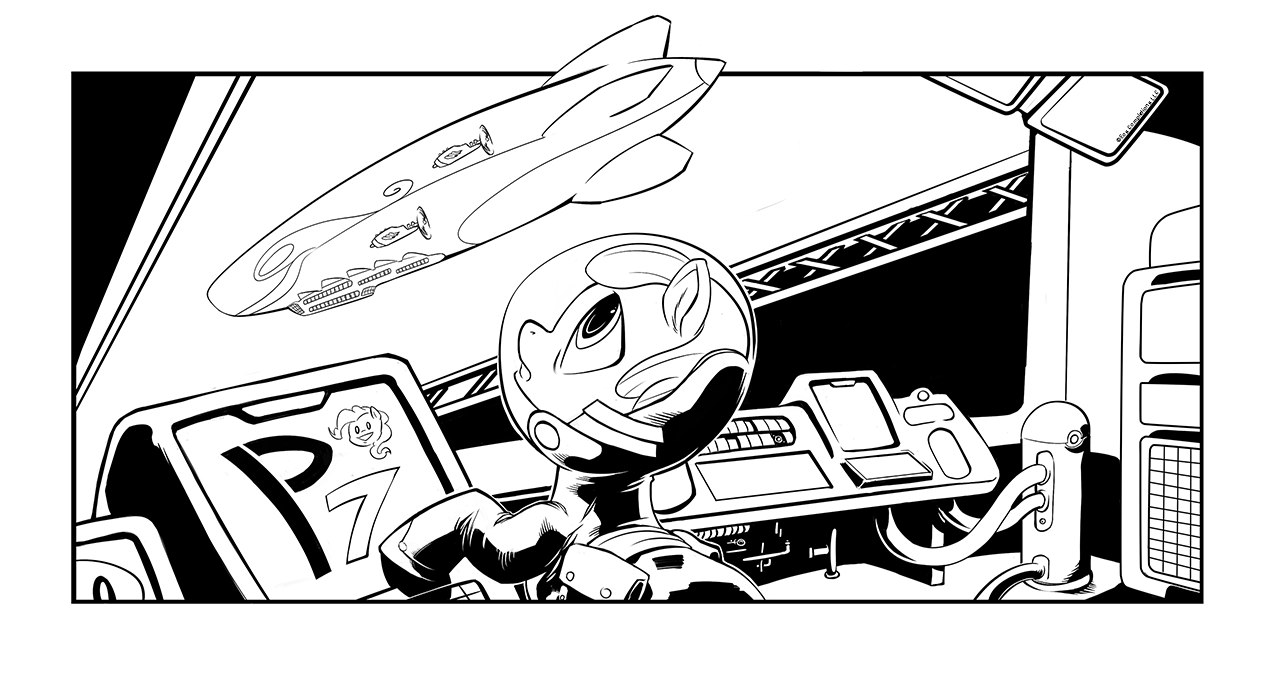
\includegraphics[width=0.9\linewidth]{image04.png}


\begin{intro}
知道吗?你们是我最好的朋友\footnote{MLP动画片头曲最后一句}!
\end{intro}

\daytimeplace{4}{3:15 PM}{炫彩大厅,盐块城}{The Glow, Salt Cube City}

「这不可能的!尸鬼是超级笨笨的吃小马僵尸!你们虽然有点丑但是你们是好马,你们肯定不是尸鬼!如果你们不告诉我尸鬼在哪,那我自己找去!哼!」帕比吐舌头。

软气和桃花相互对视了一下,然后桃花说:「我们没必要说谎啊,帕比。我们确实是尸鬼,并不是每个尸鬼都是没脑子的食马族。」

「但是他们和我说……」

「你耳朵里从来就只听你想听的话!老天啊,你是我见过最闹心的熊孩子,没有别的马这样说过你么?」桃花叹了口气,这孩子简直是选择性信息接收的典型。「醒醒吧,幽灵!这里可不是什么……充满魔法的神奇大陆,这里是小马国,没有比这里更烂的地方了!」

「但……但是……」帕比后退了一步,不知道是那个腐烂的小马,还是她现实得不能再现实的语言吓到了她。

桃花往前走一步,蹄子重重跺在地上。「别扮你的天真幼驹了!你和我们一样是怪物!别装了!行不行!?」

小雌驹吓得一屁股坐在地上,抱着脑袋把脸缩进了自己的前蹄之间。「别,别这样,我会做个乖孩子。」

「我才不需要你做乖孩子!你醒醒好么!」桃花在地上跺一把蹄子。

软气拍拍桃花的肩膀安抚道:「冷静一点桃花,我不觉得她在装模作样,冲动是魔鬼啊……」

尸鬼雌驹推开他的蹄子叫道:「她已经两百多岁了,两百多岁啊!怎么可能还这么天真?!她是智障吗?!我觉得她就是在耍我们!我们应该……」

桃子的话被一阵可怕的哭号声打断了,那一瞬间她似乎回到了自己的童年,\rcpr{那一天她把自己不小心锁进了衣柜,一直到日落之前都没有马来找她,那种孤独,被遗忘的恐惧让她拼命大叫,那天她几乎叫破了自己的嗓子都没有谁来救她}。在这令她窒息的罪恶感之中,桃子意识到帕比并没有耍他们。

所有的尸鬼转头看着那个黄色的小幼驹,她的哭号声之中似乎有着几分不自然,就好像是某种梦魇让营地里面的所有小马都感觉脊背一凉,或许这是因为那个愤怒的尸鬼在几个世纪以来第一次听到幼驹的哭声,沙盒微微迟疑了一下,然后轻轻抱起她。

「她……她到底是什么?那声音……」桃花吃惊得几乎站不稳。

「这下你把她弄哭了!」软气平铺直叙的语气说:「这回你让她相信我们是坏蛋了,干得好。」

「我勒个去,你们能不能让她别哭了?!」一只带着橙色头盔的小马抱怨着:「吵得我头都大了!」

沙盒抱着幼驹,一直到她的哭声变成低声啜泣。「好了好了,我知道你是个乖孩子,没关系的,你只是想妈妈了。」尸鬼首领搂着帕比说:「不管是谁都有脾气不好的时候,桃花姐姐很不开心,所以你道个歉她就能原谅你,不过下一次她和你解释什么事情的时候,你可以仔细听她讲话吗?」

帕比慢慢点了点头,看着沙盒那成熟的双眸,稍微找回一些宽慰。然后幼驹转头看着雌驹低下头。「我……我很抱歉没相信你说的话……桃花小姐,我现在知道你是尸鬼了,我错了。」

这个道歉让桃花的负罪感更深了,不过既然谈话现在有点进展了她也只能忍了。

「没关系小家伙,长辈说话的时候稍微注意点就好。」她顿了顿,刚刚说到哪里了「呃,我想你提到想要我们走开?为啥?」

是不是早就说过小孩子很容易分心?

小幼驹现在正挠着头盔想着这个新问题,但是却想不出一个答案。「我想……是因为那些漂漂马答应如果我来这里看看情况然后回去报告,他们就让我骑上双头牛兜风。他们似乎说过如果尸鬼都不见了就太好了。」帕比又想了想,似乎想要记起整个故事。「虽然我说已经长大了可以嘘走一两个尸鬼,但是他们还是让我发誓只是进来看看,不过因为我说的时候交叉着蹄子所以这个誓言不算数。」幼驹开心的笑着,自豪地挺起小胸脯。「我比他们聪明多了!」

软气听了笑出声来。

「赛蕾斯蒂娅哦,这个小雌驹真讨喜,我们能养她么?」

沙盒叹了口气。

「这还真是个……巧合,桃花,去找好好博士,我有几件事想和她说。软气,你能帮我看着她么?去我办公室把那个粉色玩具给这个小客人。」

\horizonline

\daytimeplace{4}{4:00 PM}{炫彩大厅,盐块城}{The Glow, Salt Cube City}

帕比爱死她的新萍琪派布偶了,一直紧紧地抱着它,时不时地秀给身边的马看。可惜在她身边的基本上只有软气。

「看到了吗?她超酷,比那杀马的机器萍琪好一百倍!而且超软!」黄色的幼驹用蹄子揉着布娃娃说:「太空服讨厌死啦!我想要亲亲它都不行!我给它起名字『丝尾』。」

「我说,小太空马,看这个!」软气敲了敲帕比的头盔说,然后举起一盘全息磁。「你猜猜这是啥?」

帕比歪着头,「呃……这个……黑色的?我知道了,是那个什么什么的什么什么!」

「我就知道,好了天才雌驹,过来让我把这个接上你的外衣。」尸鬼抬起帕比的左蹄然后打开前臂上的一个接口,把那个磁带插进去。

「{\mt 备份发现,读取中。警告,系统运行在应急模式,无法进行复制。备份拷贝结束。当系统运行正常后会打开文件。}」

「嗨,声音先生!」帕比打了招呼但是却没有得到回音。「我不知道怎么回事,好像惹声音先生不高兴了,我一来这里他就闷不吭声。」

「别担心,只是因为『盐块』,那东西影响了普通魔法晶片。」软气看着幼驹的表情笑了笑,她看起来好像在仔细听你说话,但是实际上一个字都没听进去。「那东西让声音先生打瞌睡,你们俩离开炫彩大厅之后他就醒了。」

帕比点了点头,「别告诉其他小马,我一直觉得有点寂寞……我不是说我没有朋友,而是最近几天好像一直没有马想陪我……所以……」帕比低下了头,「声音先生虽然有点笨笨的,又老是说些不知道什么意思的话,还经常发脾气,但是他从来不离开我……我只是希望他没生气。」

软气想说两句话安慰她,但是却被另外两个小马的争吵打断了。

「我们没那时间了!链式反应已经在加速了,你难道看不到吗?这东西已经变成青色了!」他听见沙盒的声音从门里传来。

「我没瞎,但是我觉得你疯了!我们还需要好几天,并不是你想的那么简单……打开圆顶然后吹起气球说拜拜!我需要时间初始化系统,然后给自动驾驶系统编程输入航线。至少要两天,不眠不休也要至少三十小时!」这是另一个雌驹的声音。

「它最多只能再坚持七八个小时了!如果我们再等下去就来不及了。」

「我真奇怪为啥这东西变化得这么快,这个破盐块在圆顶建成之前就蹲在这里了,然后现在你告诉我末日倒计时还剩下七个小时?」

帕比转头看向他们问:「发生什么事情了?」

「我不清楚,小家伙。」软气皱起眉头,这可不是什么好消息,而且也没法和她解释,就算和她解释清楚也只能让让她更惊慌。于是他说:「嘿,你想看看北边大厅的礼品店么?」

\horizonline

\daytimeplace{4}{4:45 PM}{炫彩大厅,盐块城}{The Glow, Salt Cube City}

「……这就是小马国成立的故事!」帕比说。

「啊,没错……还真是个神奇的故事,但是我刚刚想问你,你之前说的那个提问者是谁啊?」

「你说那个故事?算啦,无聊死了!我还是讲那次我不小心吃了一个蝴蝶的故事。」

软气低下了头,小声的说:「那天我在街上跑的时候,看到一个超超超超超级漂漂的……」

同时帕比也一边蹦跶着一边说:「那天我在街上跑的时候,看到一个超超超超超级漂漂的……」

\horizonline

\daytimeplace{4}{5:15 PM}{炫彩大厅,盐块城}{The Glow, Salt Cube City}

沙盒从礼品店门口探进头来,看到帕比和终于松了一口气的软气。「你们在这啊,别跑这么远,这里可能会有野生尸鬼。」

软气笑了:「别担心,我们的神奇小丫头能解决一切。」

沙盒歪了歪头:「你是说,她还被尸鬼袭击过?」

「当然,之前有那么一次,我要说这个小家伙完全能应对自如。」

「那最好,」沙盒叹了口气,「因为我真的很需要她帮忙!」

「嗨,丑丑马老大!」帕比带着开心的微笑跳到尸鬼首领面前。「我喜欢这个地方!我有个超棒的主意!我可以去告诉城里的小马,所有的『尸龟』都跑掉了,然后他们就不会来烦你们了!我们可以给你们找点漂漂衣服……然后把你们打扮成……呃……没那么丑的小马,然后改个名字,比如说鸢尾什么的!这主意超赞对吧?哦,对哦,你还需要一把长号!」

沙盒露出了微笑,那笑容有些悲伤。「我还真想试试看,不过很可惜,我是来告诉你我们要离开这里的。」

帕比的耳朵耷拉下去了:「你们真的要走?但……但是你们不能走啊!这里是你们家,而且你们又不是坏蛋,为什么要走?」帕比着急地踱着步,「等等,我还有个主意!我们可以给其他小马一个超级好的礼物,然后给他们办个派对告诉他们你们不是邪恶的!绝对可以的,绝对绝对可以的!」

沙盒叹息着用蹄子拍着帕比的头盔:「别绞尽你的小小脑汁了,这不是你的错,只是一些该做的事情,而且我需要你的帮忙才能做到。」

「沙盒,你能跟我解释一下到底发生了什么吗?我听你和好好说FFO的燃料什么的,是和我们回来的时候你们说的那件事情有关么?」

沙盒推了推他的眼镜回答:「没错,我们早知道盐块不稳定了,这么多年以来它一直以一种固定模式吸收着超聚魔法的放射线,就像我说的,在几个月之前这个模式忽然加速了,这个反应已经无法逆转,它距离完全释放能量还有不到五个小时了。」

软气沉下了脸:「好吧,这么说我们确实没多少时间了,那么怎么办?我看友谊一号(Friend Force One)还需要点维护工作,你确定这个完全释放啥的靠谱么?会释放什么?」尸鬼已经知道答案是什么了,但是他还抱着一丝希望。

「我不太清楚,可能会是比最大的斑马超聚魔法弹头还要大好几倍的魔法冲击波。那导弹打到这里的时候,这个大号盐块里面的魔法回路可不是设计用来对抗超聚魔法的,它已经尽它最大努力把盐块城的死亡宣判延迟了这么久。」

帕比想要听他们说什么,但是对话内容从一开始就听不懂了,那些花里胡哨的词汇让她觉得头晕,她甚至怀疑语言里面根本不可能有那些词。所以她决定自己去圆顶的其它地方看看。

软气伸出蹄子按住了帕比的头盔,还没等她出门就把她安稳地留了下来,老实呆在身边。

「现在FFO的导航系统还没校准,而且自动驾驶也不工作。」

「没错,不过我也没指望那东西,我要亲自飞那艘船。」

软气说话时嘴几乎是颤抖着的:「你开玩笑吧?这是自杀!而且你也不可能独自飞那东西,引擎室和氢气发生机都需要有马看着。」软气看着帕比,然后露出惊恐的表情。「难道你想让她……」

「不,别担心,她只是我们出去的门票——MK VI防护服的A.I.回路用的是和P7计划一样的东西,她只要站在里面就可以自动操作控制室。这能给我们节约很多时间。」沙盒说:「你真觉得我会把她带上么?」

「你听我说,我们其实只要撤离这个鬼地方,然后让那个盐块把苹果塔的那帮混蛋炸上天就好,我们什么都不欠他们。而且我们一出圆顶他们就开枪打我们,不是吗!我们从地道跑掉,然后让这帮家伙尝尝这个马芬的滋味。」

沙盒直视着软气的眼睛,「你想做什么做什么,我只是想让帕比去帮我打开屋顶好让我起飞,我不管我能飞多远,但是我不想再让任何一个孩子因为我不作为而死掉,我知道你恨白苹果塔那些小马,但是你难道忘记了城里的无辜妇女儿童了么?难道她们就应该当你仇恨的牺牲品?」

帕比还是想要跑,顶着软气的蹄子拼命刨着蹄子。「让我走啦,我要去外面玩啦!」

软气看着帕比,如此的天真,她甚至完全没有意识到她现在面临的灾难,就算告诉她能跑多远跑多远也没有用,如果那个超聚魔法爆炸的话……

「我去看看引擎,你告诉我该怎么做就好。」

沙盒点了点头,「我知道我可以信任你,桃花也要去,好好已经在舰桥了,我现在去教帕比该怎么做,估计要花一点时间。」尸鬼低头看着黄色的幼驹,「嘿小家伙,想去一个新地方探险么?」

\horizonline

\daytimeplace{4}{6:30 PM}{炫彩大厅,盐块城}{The Glow, Salt Cube City}

\rcpr{「再重复一次,宝贝。」}

\rcpr{「妈咪,我已经说了一亿次了!」}

\rcpr{「再说一次就好,这是一个超级特别的秘密咒语,你必须一点不错地说出来才能有用,帮妈妈个忙,好么?」}

\rcpr{「那么一会儿我能吃马芬吗?」}

\rcpr{「快要吃午餐了,如果你吃马芬的话,你也要吃苜蓿哦。」}

\rcpr{「这不公平,你总是给我一大堆那东西!」}

\rcpr{「我还会给你个超级无敌抱抱亲。」}

\rcpr{「呃……那好吧,当我在那个大圆门前面的时候,我应该把蹄子放在绿色按钮上。」}

\rcpr{「很好。」}

\rcpr{「然后那东西就会问我什么什么识辨码。然后我应该说……呃,可以提示提示我吗。」}

\rcpr{「你肯定记得,稍微仔细想想,妈咪知道你是个超级漂亮聪明的孩子。」}

{\mt 「请说出您的身份识别码。」}

「\dots FT\dots 0\dots 0\dots 1\dots 6\dots 5\dots RD\dots C\dots 1\dots G\dots A」

\rcpr{「对了,看吧,超简单,我就知道你能做到,然后呢?」}

\rcpr{「然后会问我另一个什么码?」}

{\mt 「请说出该ID的密码。」}

\rcpr{「然后你应该说……」}

「嗨,我是快乐帕比!」

{\mt 「ID接受,首席技术官阴雨·黛丝。允许进入控制室。警告,这里有三千六百九十八个错误信息需要处理。」}

\rcpr{「记住哦,如果你听到很大的喇叭声,你就要马上跑到这个秘密地方,然后用我给你的咒语,不要等我,懂了么?」}

\rcpr{「懂了,妈妈!」}

\rcpr{「我爱你帕比,过来让我抱抱……」}

这里虽然不是妈妈告诉帕比应该去的地方,不过那天听到很大的喇叭声的时候,大家都跑到外面玩去了,帕比不想自己一个人去地下……不管怎么说,这个咒语对这个门也有用。或许这个就是『芝麻开门』?

在门后面是一个超级大的房间,有很多闪亮的面板,远处的墙实际上是一大块玻璃,上面都是蜘蛛网一样的裂痕。帕比走进屋子的时候,门就在她身后关上。

「{\mt 警告,侦测到中等辐射,威胁级别:可忽略。所有系统,启动。}」

「声音先生你又回来了!我正想说……」

「{\mt 全系统工作正常,检测到通信连接请求,认证源地址。认证完毕:士气部建筑ID00201——盐块城圆顶控制室。交换通信协议……完成。警告,该防护服系统版本过于老旧。升级中,请稍候。}」

「哇哦,你还真能说,你是不是想我了!我超想你,我找到了那些要找的尸鬼了,但是他们不是坏蛋!而且他们很和善,就是有点丑……桃花训斥了我,不过的确是我的不好,所以我说对不起他们说没关系!然后软气给我一个……」

忽然一个叮叮声打断了帕比,她站在原地愣了一下之后马上去找那个有趣声音的来源。在蹦蹦跳跳一会之后,她看到在一个脏兮兮的桌子上放着一个红色的电话。帕比接起了话筒。

「您好,妈妈不在这里,我是个小孩子所以没办法做记录,您可以在晚餐的时候打来么,超超超拜托?」

「帕比,是我,沙盒。」一个熟悉的声音从电话里面传来。「看来我的黑客工具有效了,你现在也在控制室内。现在我们仍然需要点时间更换电池然后充入氢气。所以你务必要呆在那里。」

帕比看了一眼沙盒之前给她的小盒子,然后回答:「哎呀!我忘了!我没用它!」

「那你怎么……算了,没关系,仔细听好,我先要把电话关了,等我们准备好会再打过来,所以别碰任何东西,好么?」

「好的好滴好得!拜拜!」帕比把话筒放下,整个地方看起来到处都是灰土,让帕比想起那个破掉的大圆门里面,不过这里小很多,而且有很多桌子和屏幕,不过大多数都坏了。

忽然一盏红灯在坏掉的大窗户前亮起来,紧接着,更多的红灯亮起,这次几乎每张桌子上都有。几个屏幕开始闪烁着绿光。把帕比吓得一屁股坐在了地上,有点不知所措。「我可什么都没碰,对天发誓!」

「{\mt 升级完毕。P7基本客户端安装完毕,系统重启。}」

忽然整个衣服都变暗了,帕比又一次体验到了在中心城醒来那天的麻痹感觉,不过这次只持续了几秒。

「呃,这感觉好好玩……」

在帕比面前头盔的HUD上,出现一个有着七个气球的亮粉色标志,然后那个标志消失了,开始显示出普通的界面,除了顶部的罗盘以外,左右还有一大堆没用的东西,不过让帕比惊讶的是声音——不是声音先生,而是一个尖嗓子,而且听起来很友好的雌驹声音。

「嗨~!黛丝女士!我们这里有点小麻烦,所有的显示屏基本都挂了,然后我们损失了大概……100\%的职员。他们已经有多久没来上班了?哇哦……真的好久了!大佬们是不是该考虑提高一下员工福利了……哦哦,别担心!我可以在你的个人终端上操作所有东西。」

「呃,你是谁啊?声音先生去哪了?」

「我是萍琪七号!你最好的朋友,最好的小马--机器交互界面!而且我的安全程序已经写入了『不准尝试统治世界或者变成机器神明』!我很棒吧,不是吗?」

帕比挠了挠头盔,然后问:「你认识机器萍琪么?」

「哦,那当然!我们都是整个系列最先进的!她正在用于测试……呃,等等,那个测试几天之前已经完成了,我们看看结果……好像说那个测试派对实在太棒,每一个小马都爱死了!呃……不对……是真的死了么?……听起来一点都不好……好吧,我们别再提这个机器萍琪计划了,好不好,好不好?」

「但是她伤害了很多漂漂小马。」

「资料删除中……已删除,我很抱歉,我不知道你在说啥。还有其它事情么?」

「呃……机器萍琪?」帕比又问。

「没听过,还有什么事情么?」

「啊……对了,还有要飞……什么东西……」帕比戳着头盔努力在回忆。「声音先生哪里去了?我更喜欢他……」

「你……不喜欢我吗?你不做我的朋友吗?但是……为什么啊?我已经这么努力了!我已经在这里等了……大概……两个世纪啦!拜托别把我丢回服务器好么!那里又黑又孤独,我只能在那里数这里的机器做了多少次循环!拜托啊啊啊!」

「呃……如果你保证你不绑架小孩的话……」

「不会,这种事情在我的程序里面绝对被禁止了,别担心,不会有绑票!不会有大屠杀!不会有末日审判!只是帮你完成日常工作,绝对绝对不要担心!而且……我还是要说,那些安全协议真心烦死我了!」

帕比咯咯笑着:「呦呵,声音小姐也会说听起来好厉害的话!」

「没错,有时候我也……对哦,你是首席技师黛丝女士么?因为你刚才说你的名字是帕比什么的。」

「笨笨声音!我就是快乐帕比!」

「哦……棒极了,正好是我喜欢的!入侵者!在落满灰尘的魔法回路里面呆了两百年之后,终于可以玩消灭入侵者的游戏了!」声音顿了顿又说:「帕比小姐,你并没有进入这里的资格,所以我必须请你离开,虽然说你不知道这件事情有多让我伤心!」

「但……但是沙盒先生说我必须呆在这里,不然友谊飞船就飞不起来!我能再呆一会吗,拜托,超超拜托,漂漂拜托?」

「如果你想呆在这里的话,你必须证明你至少是个军队的上校或者士官什么的,我真的……真的……真的很想让你陪我,但是我必须秉公无私!除非我有什么事情在忙,比如说一个逻辑悖论或者有趣的死循环\footnote{逻辑悖论与死循环:许多科幻小说中弄坏人工智能的惯用桥段}什么的……哦,等等!你和首席技师是什么关系?」

「谁?」

「阴雨·黛丝!」

「哦,她是我妈妈!你知道她在哪里吗?」

「不知道,但是这解决了大问题,让我看看啊,把这个弄到这里,这个到这里这个这个……妥了!今天是带女儿参观工作场所日!你开心吗?」

「呃……我想要妈妈。」

「喏,你看,这个事情都写在你的任务清单里面!你真的想要找你妈妈,是吧!」

「那当然,那是我妈妈!」帕比板起脸。

「你跟我说,我们可以……哦哦哦,等等,紧急路线有一个电话!」

沙盒的声音代替了那个A.I.的声音。

「帕比我们准备完了,你那边如何?」

「嗨,老大,我当然没问题,这个声音小姐真能聊。」

「真棒,现在仔细听好,有几个小马想和你道个别,乖乖听着,不会有多长时间,毕竟我们有点迟了。」

沙盒的声音又被桃花代替。

「喂,小家伙,你在吗?」

「嗨,桃花小姐。」

「我很高兴听到你的声音,我想说……对不起,我其实没必要训斥你……我们可以和好吗?」

「呃……没关系?」

尸鬼雌驹长舒一口气:「感谢赛蕾斯蒂娅,心里放着这事,我什么也干不了,请记住我的话,帕比,小马国是个不可原谅的地方,你必须相信你的朋友,因为在这里你很难交到朋友。我……我很后悔我们没时间相互加深理解,但是只要知道你很安全的话,我想我也就无怨无悔了。」

「你要走吗?你到那边之后我能去见你吗,好吗?我们可以开一个派对!」

桃花沉默了一会,然后回答:「可以……可以的帕比!如果我们有缘再见的话,我们会开一个超级大的派……抱歉,我离开一会儿……」

电话沉默一会之后,另一个声音响了起来,「嘿,帕比,我是软气,请听从沙盒指示哦,我们全看你的了!」

「软气!声音先生现在变声音小姐了,你说有趣不有趣?」

「你在说什么……算了,没关系,我想和你说件事情!我认识你的妈妈,不过别惊慌,我时间不多,你仔细听好。」

「你……你为啥不早和我说啊!」

「我想……我想早点说,但是这个超聚魔法让我忙得晕头转向,你现在听我说,我曾经是她的手下,第三装甲师『铁壁』的三等技术士官软气。你记得我给你的那个磁带吗?」

「呃……那个黑色的那个什么什么的什么什么?」帕比努力回忆着。

「对,就是那个,那里有我们长官的位置,大概就在盐块城南边,在沼泽那里,如果你想找到长官线索的话,那边一定有。所以在你把控制室的事情弄完之后,把165战指设为主要目标,然后跟着粉色箭头就好,你明白了么!」

「我……嗯,明白了,去指挥部,找妈妈!谢谢你软气,你是最棒的小马!」

「我想你是在说『萍琪派』吧。」P7打岔。

「还有最后一件事,帕比,你的旅途之中一定会知道一些让你伤心的事情,那是不可避免的,但是我知道你是个勇敢的孩子……所以,拜托,别忘记超聚魔法落下之前的那些日子,小马国现在是一片荒芜的死亡大陆,但是你知道这里不可能永远像这样荒芜下去!不要让废土侵蚀你内心深处的纯真!我会在太阳照耀天空之前一直看着你的!」

「呃……为什么大家都说这些伤心难懂的话?你们只是去坐个小飞机,又不是我们永远见不到了,我和妈妈会在你们找到新家之后再去看你们的。」

「帕比,这里是沙盒,你还在听我么?」尸鬼长者的声音打断了对话。

「啊……是的老大……你说,我们还会再见面吧,对吧?」

在一阵长长的沉默之后,尸鬼平静而又悲伤的声音说:「我相信,我们会在彼岸的尽头再一次相聚,如果你想再见面的话,请不要失去希望,帕比。」在另一阵沉默之后,尸鬼长官又开始说:「我们需要你打开屋顶好让我们起飞。现在,你重复我的话:『启动语音控制,授权码SB01,首席研究员,密码:阿加莎。改写协议01-11的优先权……』」

\horizonline

\daytimeplace{4}{7:30 PM}{闹市区,盐块城}{Downtown, Salt Cube City}

灌木正坐在窗户边用狙击步枪守卫着圆顶方向,他已经值班很久了,而且天色渐渐变暗,再过一个小时他就要挪窝下去了,希望下面能有一碗热燕麦粥等他。

「我很好奇为什么他们送那个小丫头自己去圆顶……她连午餐都没吃就进去了。可怜的小家伙,我们现在都开始让孩子去送死了……」小马一边启动瞄准镜的夜视功能一边喃喃自语。

就在那个时候,圆顶东边还完好的部分随着一阵金属的摩擦声开始坍塌下来。

「露娜我娘亲哦!那里怎么了?」卫兵用瞄准镜看着那里发生了什么。

在观察几分钟之后,士官确定房顶并不是真的在坍塌,不完全是,那里的确有很多灰尘和零件落下来,但是建筑的东边实际上是在……旋转?经过两百年的风吹雨淋,整个圆顶早就快锈成一块铁疙瘩了。但是现在有什么巨大的力量正扯开那些不想动的铁板。在被轰炸那天之后就被忘记的钢铁老古董在一阵金属哀嚎声中裂成好几块。

不管怎么说,房顶依然慢慢移动着,虽然对自己的结构造成巨大伤害,但仍然旋转开来。现在那堆垃圾的最后一片也消失了,『圆顶』完全滑到了一边,露出一个像城镇广场那么大的空间。

那个噪音让闹市区的所有小马都抬起了头,有些雌驹当场就吓昏了过去,倒下前还大叫着「好可怕,好可怕\footnote{好可怕好可怕(The horror! The horror!):\emph{MLP} 动画里面鲜花三姐妹吓得满街跑时的惯用语}!」之类的话,但是不为所动的士官依然冷静地举枪瞄准那个大洞。

「好了,尸鬼,让我们看看你们腐烂的脑袋里面装了什么。」

在房顶一阵金属摩擦声中停止移动的同时,另一半房顶也停了下来。然后整个天空被数千盏粉色的探照灯照得一片明亮,随着又一阵蓝色和绿色的烟雾和亮片从圆顶周围喷上天空,一个尖嗓子的声音开始喊话了。

「女士们,先生们!」声音从圆顶的喇叭里面传出来,虽然带了很多杂音,而且一个喇叭似乎坏了。

「为我们伟大的赛蕾斯蒂娅公主和露娜公主献上我们最诚挚的敬意!我在这里心中满怀荣耀地向你们介绍我们最尖端,最神奇的最新大型交通工具!『友谊一号』!她让小马国交通更加便利!」

然后是一阵音乐声。

「现在让我们介绍嘉宾!首席技师黛丝女士的女儿,快乐帕比!」

「……然后我说道:『燕麦粥,你疯了么?』接着是一阵沉默。呃……那是我的声音么?啦啦啦啦啦啦~!呀,真的是!太有趣了,再见尸鬼们,祝你们旅途愉快,给我寄明信片哦!」

士官灌木抬起了眉毛,「到底发生什么了,首席什么黛?谁是黛丝女士?而且那个……我……去……是……什么?」

在打开的圆顶中,一个形状奇怪的东西慢慢升了起来,它看起来像是一个气球,但是却非常长,看起来像是一根尾巴很粗的巨大玉米棒,在两边还写着『友谊是魔法』的大字。

士官揉了揉眼睛,把自己掉下来的下巴用蹄子合上,现在那艘飞空艇已经从圆顶升了起来,然后慢慢转向,在那个粉色的巨型气球下面是一个类似天空马车\footnote{天空马车(Airwagon):\emph{FoE} 设定中天马可以拉着飞的马车,可以靠天马的魔力悬浮在空中}的东西,但是大好几倍,在身边伸出的两片鱼鳍一样的翅膀,后面还有好几个螺旋桨。

然后这东西开始加速,避开塔尖,朝东南方向飞去。士官满脸难以置信地看着那气球飞走,那个尖嗓子声音还在喊着。

「非常好,这是士气部给你们带来的表演,大家,记得买战争基金哦!而且记住,你们不开心萍琪派也不会开心!所以微笑吧!因为她会永远注视着你们,永远永远哦!」

当圆顶的灯光和音乐都消失的时候,气球已经飞了快一公里远了。圆顶想要再关上,但是却只是带出一阵新的金属摩擦声,然后变成了一堆碎片。

「我勒……个……大……公主……啊……他们……他们……就这么……坐上那东西……跑了?」卫兵挠着头,「为什么早不走?而且他们从哪儿弄来那滑稽的东西?友谊是魔法?简直疯了!」

% NOTE: ignore overfull

\horizonline

大概一个半小时之后,小马们都回去睡觉了,飞空艇也成了远处天空的小点,早已经在几十公里外了,不过比起天空马车来说真的飞得不快,不过它非常大。

楼梯上传来的马蹄的声音让灌木士官警觉地竖起耳朵,不过他的视线还在飞走的气球上。

一只穿着战斗鞍具的雌驹敲了敲墙,然后走进屋子。「该换班了,伙计,刚才是不是很精彩。」

卫兵转头看着他的战友。「他们……就那么飞走了?那么大一气球……我不明白,为啥要飞走?」

雌驹看着外面,然后问道:「喂,你没觉得少了点什么吗?」

「对,尸鬼和剩下的圆顶屋顶都不见了。」

「不,我不是想说这个,你看,那炫光也不见了。」

「哎呦我去!你还真说对了,圆顶不发光了!看起来黑黑的……闹鬼一样,真有点毛骨悚然的……」

「所以,他们真的走了?明天早上天亮之后我们去检查一下辐射剂量。」

「你觉得……」忽然整个世界都被漂白了。炫目的光芒让士官睁不开眼睛,他一直到光亮消失之后才看清发生了……

轰隆!

这是他听过最大的声音,就像暴风之中的惊雷一般,而且更大声。卫兵立刻抓着他的战友卧倒在墙后面。

下一瞬间强大的震动和一堵烟尘的巨墙袭击了闹市区,把无数窝棚都弄成碎片,只剩下几个坚固的建筑。

「那……那是什么?」士官拼命想睁开眼睛。

「我不知道……尸鬼的飞天机器爆炸了?看起来像是什么巨大的……」然后雌驹意识到了那是什么。「哦我的赛拉丝蒂亚啊!是超聚魔法!他们飞的那东西上带着一颗核弹头!」

~\vfill

\begin{note}
    升级(Lv 3)

    新专长解锁:应急训练——魅力($7 \to 8$)现在你比之前要酷了14.28\%!
\end{note}



\chapter{小鸡}

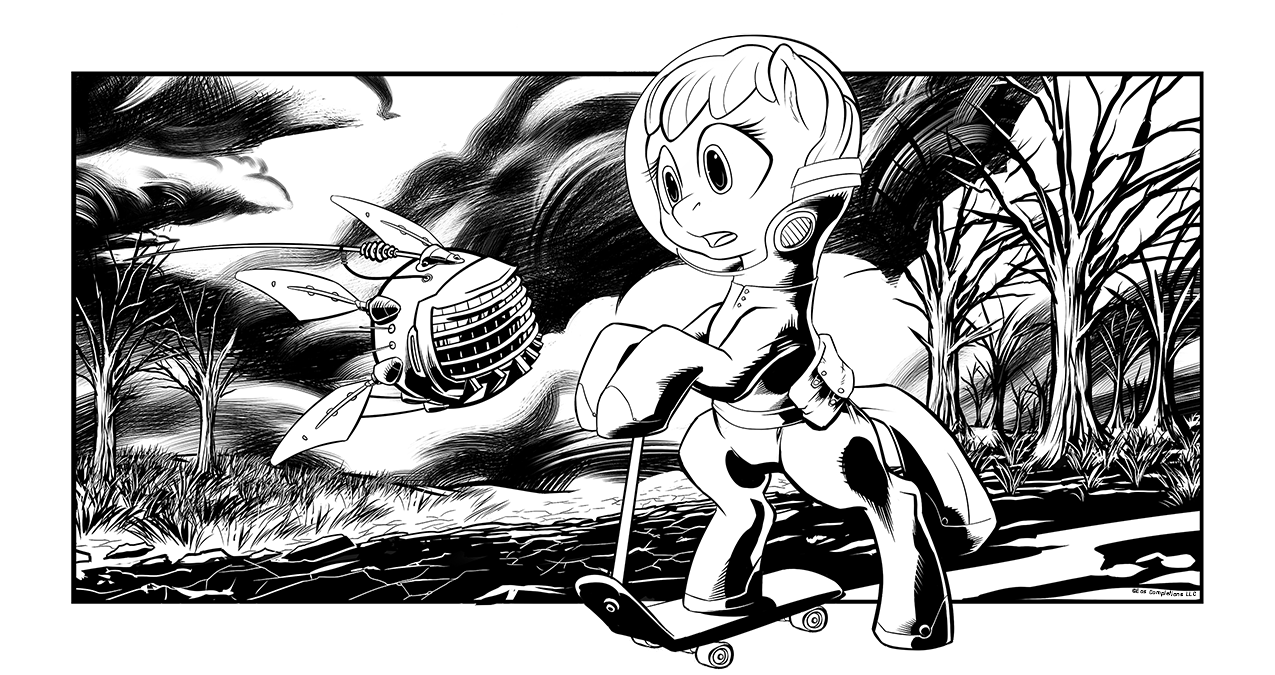
\includegraphics[width=0.9\linewidth]{image05.png}

\begin{intro}
可爱标记童子军小鸡营救队来了!
\end{intro}

\daytimeplace{5}{9:30 AM}{闹市区,盐块城}{Downtown, Salt Cube City}

「耶!漂漂牛快点!再快点!」

双头牛左边那个脑袋重重叹了口气,然后一脸绝望地望向旁边带着黑帽子的独角兽。

那小马对牛无奈地笑了笑,挥着蹄子打断她无声的抱怨:「这是交易的一部分,别不满意啦,再让这个幼驹骑最后一圈,然后带她来我办公室。」

「好,好,白先生。」牛不爽地在白塔外面转来转去,在之前的半小时她们已经跑了好几圈了。虽然外面的小马都在忙着修理昨晚冲击波造成的破坏,但是被一个黄色小雌驹骑着还是会引来很多好奇的目光和窃窃私语。

「我认得她,是嘉年华的幽灵……她诅咒了那些尸鬼,这个孩子一定会带来厄运……」

「你看,她在白塔外面装傻,我敢用我的所有瓶盖打赌,她一定用她在圆顶里面看到的东西来威胁他们呢!」

「你没看到吗?圆顶的炫彩已经消失了,然后……然后尸鬼的飞船也爆炸了!他们肯定想搞什么鬼,结果反而坑了自己。可恶的尸鬼,他们就是活该!」

「但是……她到底是谁?」

「别问,我从来没看见她吃过东西,甚至没看见她打开自己的头盔,虽然不知道怎么回事,不过她绝对不是好东西。」

「别说了,她过来了!」

帕比自己玩得很开心,完全没有去留意那些窃窃私语,「太棒了,超超超有趣,牛小姐们,我们有时间再玩一次好吗?」

双头牛的其中一个脑袋点了点头,「当然,不过你要先问问白先生,他在办公室等你,就在红色的门里面。」而另一个头一脸不爽地继续反刍着。

白先生的办公室很大,很整洁,墙上挂了很多照片,而地板亮得可以照见自己的影子。

「哇哇哇!这个地方真的超超超漂漂!」

白苹果的老大是一只戴着黑帽子的雄性独角兽,毛皮是白色,鬃毛是天蓝色。「嗯,谢谢夸奖,黛丝小姐。」这个称呼似乎让帕比愣住了,所以白先生又说:「那个圆顶的声音昨晚不是说你妈妈是阴雨·黛丝吗,所以你的全名是快乐帕比·黛丝,是吧?」

帕比歪了歪头,最后又点了点头,「嗯,没错。现在我该走了……声音小姐在我的罗盘上显示了一个箭头,所以我该往那个方向走了。我可以走了吗?拜托。」

老白叹了口气,压低帽子挡住了他的眼睛。「当然,没问题……但是……我还是想问你最后一件事情。圆顶里面以前是什么东西在发光?」

「你是说盐块吗?」帕比就像听到什么有趣问题而咯咯笑起来。「你好笨哦,我是说,你不是一直住在盐块城嘛,你居然都不知道盐块,真是……」

那个老马正要大声训那个小雌驹,但是仔细想想和小孩子闹脾气又没什么用,所以他只是笑了笑。「我承认我一直没去过圆顶,那里有点……可怕,所以,是尸鬼把那个盐块带上他们的飞船了吗?」看着幼驹一脸迷茫,于是他补充道。「就是那能飞的气球。」

帕比点了点头。「没错!他们看起来超级着急的样子!他们都说会什么……盒爆?……核包……啥的?」帕比看起来不是很开心的样子,「反正是什么什么东西,我记不太清楚了,但是他们说他们要在发生之前走得远远的,因为很危险?」

「核爆?是这个吗?」

「对!他们说因为链啥反应……反正就是那个方块要赶紧丢得远远的,我还帮他们了!」

蓝色鬃毛的小马一脸惊讶,「他们……想要带着那炸弹走得越快越好?我……我知道那些尸鬼都是疯子,但是他们居然……好吧……我想这解释了为什么圆顶的光消失之后放射性几乎消失了。」

白先生露出放心的笑容,「你干得很好,小家伙,我很想再招待你一会儿,但是你这么急着走的话,至少让我送你出门。」

「好的好的!白先生!拜拜!我会告诉我妈妈你对我很好!」

「好,一路顺风小家伙,很抱歉我有些好奇,你想去哪?」

帕比指着南边说:「那里!妈咪就在箭头的终点!」

「哦,直接去沼泽地啊……祝你好运!」

她死定了。

这个沼泽是52号国道北边最危险最糟糕的区域。这个幼驹只会变成某个废土强盗的早餐。虽然很可惜浪费了这么好的防辐射服,但是白苹果家族不是强盗。

白先生沉思了一会,回忆着昨晚的事情,虽然这小姑娘就要走了,但是这样利用一个小孩子,让他后悔不已。她或许拯救了整个盐块城,但是他又给了这个孩子什么回报呢?只是骑着牛跑两圈?她就要遭遇危险了,而他甚至连一点建议都没有?这太不公平了。

「喂!黛丝小姐!等一等!我有东西送给你!」

\horizonline

\daytimeplace{5}{11:30 AM}{盐块城外,52号国道北部}{Salt Cube City Outskirts, Big 52 N Branch}

「呀……呵……!」一颗踩着红色滑板车的黄色子弹飞驰在公路上。

盐块城的建筑早已远远甩在脑后,路边的景象又变成了一片荒芜的废弃农田。

% NOTE: 遵照英文发布版改

\rcpr{仔细听我说,你到了乐麦镇之后,就绕道,穿过沼泽的路——}怎么怎么怎么怎么\rcpr{——一定要记住,绝不要穿过}什么什么什么……一些无聊的东西,帕比已经记不清了!

幼驹骑着滑板车嗖嗖地飞驰向南方,似乎是觉得滑板车的声音不够刺激,帕比还自己加上音效。「呜呜……嘟嘟……!飞向月球!宇宙无限!太空战士安德洛队长拯救世界!耶!」

在黄色幼驹面前,路上都是腐烂的田地和荒芜的农场,盯着箭头走了一会之后,农田变成了枯萎的果林和满是泥水的水坑。偶尔会有一两个营地,但是看起来已经遗弃很久了。虽然还有一点点生命迹象,但是都是一些昆虫或者不敢惹帕比的野兽。

唯一敢于接近帕比的,是一个飘在路中间的机器精灵。

「嘀嘀,我是吉普车!太空战士来啦!」帕比在玩疯的时候从来不会注意细节,黄色子弹继续以最高速度飞驰着。机械精灵在被撞上的前一瞬间连忙躲开,然后又急忙追着帕比飞。

「嗨,帕比,这么急着去哪儿啊?」一个熟悉的声音从喇叭里面传出来。

「提问者!我好想你!快看我的新滑板车!」帕比一边全速前进一边咯咯笑着,「我还认识另一个说话机器,不过那个很有趣,或许她不是一个机器?我不确定。」

「真有趣,可以和我讲吗?」机器精灵没等回答就接着问。「昨晚盐块城发生了什么?那个大爆炸是怎么回事,圆顶怎么了?你能停一下么,拜托!」

帕比叹了口气然后开始减速。「真会挑时候,人家正玩得开心呢……」

停下来之后,幼驹跳下滑板车,她一边想着守望者的问题,一边敲着头盔下面下巴的位置。「你是问圆顶?我在那里交了好多朋友!老大沙盒,软气先生,桃花小姐……哦哦,还有声音小姐!」

「不是声音先生了?」

「不对,傻机器,有一个声音先生,还有一个声音小姐!她住在圆顶但是声音先生可以随时叫她来,她超级酷而且帮我给尸鬼们办了一个送别派对!」

「哦,另一个小马--机器智能交互界面么……那么……你见到了尸鬼,还办了一个送别派对?你是什么意思?你帮他们发射的飞船?」

「太对了!」帕比兴奋地点着头。「超超超超级棒!我从窗口看到一个大大大大的东西高高高高地飞上天!」帕比举起前蹄描述那东西飞得多高,但是举过头了让自己一屁股坐在了地上,她咯咯笑着坐正了继续说。「然后好多好多灯照得雪亮雪亮的!我听到我的声音超超超超级大,所以我说『啦啦啦……拜拜尸鬼』然后他们就飞走啦!超级酷!滑板酷!」

「滑板什么?」

「滑板酷!」

「有这说法吗?」

「当然滑板!」

「你知道么……显然那滑板对你的小脑袋没什么好处……」守望者的声音听起来有点担心,「好吧,扯远了,那爆炸是怎么回事?」

「什么爆炸?」帕比不解的歪着头。「你说房顶又塌了?」

「不是,我是……等等……又有房顶砸你脑袋上?」这句话很明显让守望者有些惊讶。

「没错,那个房顶打开,然后大气球飞走之后,整个地方嘎吱,然后咣当!正好掉我头上。」帕比咯咯笑着,「但是我是一个超级太空小马,所以我把自己挖出来了……我就是那么厉害!」幼驹自豪地笑着。

机器的喇叭里面传出一阵笑声,然后又是一个叹息。「好吧,现在你要去哪儿?」

「当然是下一个妈妈地点!很明显,第三次会交好运!」

乒!乒!

忽然一阵枪声在空中响过,不过子弹明显不是向着帕比或者守望者来的,但是幼驹很明显听到了声音。「那是啥?」

「我……很抱歉帕比,我该走了,附近可能有强盗,你最好躲起来等他们火拼结束。」

「火烧?哪有?我要吃!」帕比蹦蹦跳跳地四处张望起来。

「塞拉斯蒂娅公主,请务必保佑她安全……」机器精灵的声音被一阵音乐代替之后,那个无人机飞走了。

声音是从帕比头上传来的,小幼驹抬头看的时候,看到令她难以置信的景象:有些超级大的飞天小马一边放着烟花一边飞来飞去,就像超华丽的芭蕾舞。这个场景让帕比回想起那天妈妈带她去飞行场看漂漂天马在天上做超级有趣的表演。

这次看起来也差不多,虽然有点不同的是飞在天上的小马不停地在闪光并且发出很大响声,帕比马上觉得这一定是他们最喜欢玩的娱乐项目。

但是她马上发现那些大家伙不是天马,所以幼驹皱着眉头问道:「我说,声音先生……那些小马生病了吗?」

「{\mt 分析中。友善的狮鹫。}」

虽然帕比一点都不明白狮鹫是什么,但是如果声音先生说那是『友善』,那么都可以啦。黄色幼驹挥着蹄子大喊起来。「喂!漂漂马!我在这里!喂喂!」

其中一个生物转头看了地面一眼,然后放松警惕的它马上就被另一个生物击中,然后打着转栽了下来。

「呃……我看看……一……二……三……呃……」帕比想数一数有几个狮鹫,但是他们飞得太快,所以她还是跑向那个倒在地上的家伙身边,幼驹注意到她根本不是小马,看起来像是某种半鹰半狮的奇怪生物——她觉得那东西看起来真滑稽。

「我说,小鸡先生!」

那生物一动不动,一大滩血正在他身体下面慢慢扩展,帕比用蹄子戳了他一下。「喂,怎么啦?」

没有反应。

「呃,小鸡先生?起床啦?太阳高高哦!」

依然没有任何反应,这看起来可不太妙。不过最糟糕的是他的朋友似乎根本没注意到这边的情况,所以她该做点什么。

「喂!小鸡们!你们朋友受伤了!快下来啊!」帕比用自己最大声音,挥舞着双蹄大喊着,但是很明显她被忽略了。那剩下的三只狮鹫还在天上跳着华尔兹,不断有血从天上洒落到她头上。

「唉,他们玩得太开心不理人家!」帕比叹了口气。「如果我能有什么东西吸引他们注……等等,我有!」幼驹微笑的想起那个白先生给她的那个闪闪东西,那叫什么来着,揪毫民?九耗毛?「呃……声音先生,给我那个闪闪发光还很聒噪的东西!」

「{\mt 警告,物品『快乐帕比』不能从物品栏中取出。}」

「喂喂!你这样不对吧!你知道我说什么!那东西,那个揪毫毛什么的!白先生给我的那个!」

「{\mt 肯定,取出『九毫米半自动手枪』。}」

枪飞到了帕比面前。幼驹把这个铁块握在蹄子上举向天空。「喂!喂喂!喂喂喂喂!听我说啊!这东西怎么用?怎么发出声音?」

「{\mt 读取介绍中……射击模式『危急时刻』!首先,将枪指向目标,然后,说出『开火』或者『啪』,枪就会击发。如果想要装填的话,将武器放入物品栏再取出即可。}」

「呃,听起来超简单。」帕比指着狮鹫,「啪!」

乒……

% NOTE: 呯 -> 乒

「哎呦!」

后坐力让枪从帕比蹄子上飞出,砸在她头盔上让她坐了一个屁股蹲,然后落在了不远处。

其中一个狮鹫痛得大叫起来。「见鬼!他有后援!杀了那个傻……」他还没说完,他的头就爆成了一团血雾。现在天上只剩下了两只狮鹫,战斗变成了一对一的厮杀。

两只狮鹫冲撞在一起,用喙和爪子又撕又咬,帕比走到那个落下来的狮鹫身边,看到他的头不见了。「你知道吗,声音先生……我觉得他们不是在玩。这个小鸡……呃……死了?」

「{\mt 肯定。}」

「呃……嗯……」帕比皱起眉头。「另一个呢?」帕比指着地面说:「他也死了?」

「{\mt 分析中,没有生命特征。目标已死亡。}」

帕比又看向天空那俩纠缠在一起的狮鹫。「他们俩……在相互伤害对方?」

「{\mt 肯定,每一条线索都表明他们在死斗。}」

「好吧……」帕比想了想,然后说:「我怎么让他们停下呢?哦,我有点子了!」帕比深吸一口气:「拜托请别打架了!某马会受伤啊!」

实际上某马已经受伤了,或者说,某狮鹫,但是帕比并不太清楚幸存的俩斗士什么情况,他们似乎完全没有注意帕比,但是其中之一忽然发出一声尖叫,然后他们一起打着转从天上栽下来。

帕比跳上滑板立刻追了过去,想看他们落在哪里,等她到那里的时候,看到其中一只狮鹫胸口被抓开,喉咙也有一个血窟窿,而另一个尝试站起来的狮鹫身上的好几个伤口都在流血。

「小鸡先生,你还好吗?」幼驹飞奔到那个想要站起来的狮鹫身边,但是他却倒在了地上咳嗽着。「你看起来不太好。」

「咳咳……你就是开枪的那个……谢谢……」

帕比皱了皱眉,「我……是啥?」

「咳……咳……听我说……我……我女儿……在……南边……军营……咳咳……」狮鹫痛苦的喘息着,「赫瑞塔……她……在那等我……咳咳……求你……去……把这个……给她……」狮鹫递给帕比另一只枪,这支枪比她的那一把重多了,而且表面是全黑的,枪口还有一条红线装饰。

% NOTE: ignore overfull

「呃……好的?」帕比戳了戳狮鹫,「没问题……但是……你会好起来吧……是吧!」

「你……你是笨还是……我要死了……」他咳出一口血打断了他的话,「告……告诉……赫瑞塔……我……我要她……往南……告诉她……我…………我……告诉……」随着最后一丝光芒从狮鹫眼中消失,他的声音也同样消失了。

帕比等了一会,然后又用蹄子戳着狮鹫,「嘿,小鸡先生,你睡着了?小鸡?」她又戳了戳他。「呃……我想……我该走了……我……呃……很抱歉……」幼驹从死去的生物前后退了一步,她感觉很糟糕,有什么东西完全不对。虽然不是第一次看到死去或者正在死去的生物,但是……她从来没有像这样仔细注视过。

如果说现在是个证明「这个世界上小马都是相互杀害对方而求生」的好机会的话,对于帕比来说这只是个伤心的故事。

「呃……我希望你能好起来,不过现在我真的……真的真的……要走了,抱歉……」幼驹透过头盔吻别狮鹫之后。跳上她的滑板跑远了。

「声音先生,你在吗?」

「{\mt 肯定,系统一切正常。}」

「为什么漂漂小马都要互相伤害?」幼驹皱眉问。

「{\mt 警告,该程序并没有社交功能。}」

帕比叹了口气继续顺着粉色箭头往前走。「呃,声音先生……那个小鸡说什么女儿的事情?」

「{\mt 肯定。已经被设为次要任务目标:坏消息,新伙计。}」

帕比犹豫了一会之后停下滑板车说:「你能告诉我她在哪吗?」

「{\mt 肯定:赫瑞塔·火红(Henrietta Firebright)设为新的目标地点。}」

帕比看了看那消失然后又出现在同一个方向的粉色箭头。「呃……我觉得没设对吧?」

「{\mt 否定,新目标已经正确校准。}」

帕比叹了口气,操作这个奇奇妙妙的太空服是声音先生的工作,如果他说没问题,那么就没问题。

「我们走。」

\horizonline

\daytimeplace{5}{14:00 PM}{165战指附近,盐泥沼泽}{165Th Brigade field Headquarter, Salt Marshes}

「{\mt 警告,密封多处破损。警告,罗盘失灵。警告,无线电离线。警告,医疗系统离线。警告,头盔破损。警告,粉色药剂发现。维修回路启动。}」

「呃……我觉得……我是不是踩到什么了……」帕比想站起来但是又摔倒了。「晕晕乎乎……」

在幼驹面前的一堆路标写着『注意,雷区』和『军事管制区,禁止通行』在她身边落了一大堆沥青碎片,而她面前的路面少了一大块。不过那个滑板车却奇迹一般倒在幼驹身边,毫发无伤。

「唔……声音先生,为什么路面嘣地炸了?」她身上的每一个破洞都包裹着粉雾。

「{\mt 分析中,爆炸原因是地雷。无线电恢复,头盔修复。}」

帕比皱了皱眉头,「什么是地雷?等等!你总是这样!说好多听起来很厉害可是我却听不懂的话,那样我就没法因为你说错了什么对你生气了,是吧?我要专家来帮忙!叫声音小姐来!」

「{\mt 开启通讯连接,请稍候,罗盘恢复正常,医疗系统上线,读取目标001号个性化信息:快乐帕比,目标已死亡,状态稳定,完毕。}」

不到五分钟防护服就完全修理完了,修理用的基本都是帕比捡进口袋的各种垃圾,幼驹对她身上装的东西没什么选择性,只要五颜六色还闪闪放光就捡起来,而自我修复魔法也没什么要求,任何包括金属,玻璃,塑料的材料都可以。

「喂,喂喂?这里是盐块城圆顶紧急线路,很抱歉但是现在所有职员都已经死了,请等服务恢复以后再联系,拜拜!」

「等等,声音小姐,是我,帕比!」

「哦,帕比!你好,好久不见,你去哪了?你找到我让你找的东西了么!我的迁移协议随时准备就绪。」

「呃……没,抱歉,声音小姐,实际上,我需要帮助。」

「哦,别担心,我会在这里等你,反正都两百年了,再等几个世纪也没关系!所以,你想要啥?」

「呃,我正像神奇天马一样骑着我的新滑板……」

「等等等!你有一个新滑板?是红的?」

「那是当然的啦!」

「滑板酷!它很快,超快,还是超超超超快?」

「坐在上面就像坐火箭一样所有东西都嗖嗖往后走!你真应该试试看,超疯狂!」

「我真想试试看,你给我找个原型身体我就可以试试看,一言为定哦!」

「当然,萍琪毒誓!」帕比想要拍自己的眼睛但是被头盔挡住了。

「耶!好了,扯远了,你打电话来是想跟我炫耀新滑板的?」

「呃……不是……实际上我遇上了会爆炸的路……你看,声音先生跟我说什么地瓜啥的,但是我觉得地瓜应该很好吃而且不会爆炸。」

「哦,那取决于地瓜的品种,不过我想我知道你想说什么了,地面爆炸了而且不知道地雷在哪里……现在请你看看附近,有没有类似大号扁平飞盘而且上面亮白灯的东西,或者也可能是难看绿或者恶心黄……」

帕比笑了起来,「对对对!我看到了!等等……有好多好多!满地都是!就好像一大堆萤火虫,赞哦!」

「哦,我知道你说的地瓜是什么了,没关系,我要亲自看一下,等一下!」头盔的HUD闪了闪光之后,整个头盔都亮起了目标信号,每一个地雷的位置都标记了出来。「哇哦,四十五个,还有更多!这让我想起了我平时玩了很多很多次的那个游戏。」P7稍微顿了一下,等待整个雷区扫描结束。

「完成!现在我规划出一条路径,你只要照我说的那么走,就可以顺利到对面啦!」

\horizonline

\daytimeplace{5}{11:45 PM}{165战指附近,盐泥沼泽}{165Th Brigade field Headquarter, Salt Marshes}

这个基地看起来毫发无损,一排巨大的机库在一个大院面前,附近还有好多小碉堡,前面有一对自动防御机枪,但是一辆大号坦克压烂了它。几乎把整个大门都撞垮了,只留下一条能让一只小马勉强进去的缝隙。

帕比呆呆地看了一会,然后兴奋地爬进坦克之中。

「哇啊!这东西装满了亮闪闪的东西!瞧这个!」幼驹拿起一颗弹头有红条的炮弹,看起来很大,估计是坦克的主炮弹药。「真漂亮,喂!那还有好多!这个是黑色,还有蓝色,呦呵!」

在拆了坦克的弹药箱之后,帕比终于想起了正事。她走进基地,庭院中还有更多坦克,但基本全都丢在那里,被沼泽的湿气锈烂了,各种奇怪的植物从窗户里面冒出来,帕比似乎没看到狮鹫女儿的迹象,所以她做了她觉得最合理的事情。

「咕咕……咕咕……咕咕……咕咕……咕咕……咕咕……咯咯哒……咯咯哒……咯咯哒!」还是没反应,真奇怪。「或许她睡了?」

% NOTE: ignore overfull

「{\mt 警告,发现敌对生物,距离 \SI{100}{m}。}」

一个巨大的生物从一所小屋里面露出头来,看起来是某种狮子,但是却大很多,而且还有一对皮膜翅膀和一条刺针上滴着毒液的长长蝎子尾巴。

「{\mt 分析中。蝎尾狮,威胁等级:致命。}」

「呃……那不是我要找的小鸡。」帕比转头走向那个野兽,完全不管警告。或许他知道那个女孩呢。

「嗨,我是快乐帕比!你看到我妈妈或者有个漂亮小猫尾巴的小鸡吗?」

那头巨兽低头看着小小马,嗅了嗅之后,低吼着后退了几步,看起来是被快乐帕比吓到了。

「你听到我说话了吗?拜托,超拜托!加樱桃的拜托!她有俩翅膀,一个喙,而且很小,呃……不知道她有多小,不过我想她应该很小,你在听我说话么漂漂猫猫?」

蝎尾狮吼着拍了帕比一爪子,把她打出10米多远,然后转头走进了半毁的建筑中,等在地上滚来滚去的帕比站起来之后,她对那个野兽的巢穴吐了吐舌头。「呸呸呸,坏猫!我自己找小鸡去!」幼驹皱着眉头,「真是的,这里的动物都这么漂漂,为啥小鸡要躲起来?」

帕比走进另一个看起来完好的小建筑,她探头进去。「呃,有马在吗?」她看到一面点亮的电脑屏幕,幼驹走进屋子,看到这里是个小办公室,还有几张桌子和一排柜子,在电脑上显示着一行字:「{\mt 请输入密码。}」

我有没有说过帕比基本上不识字?「亲……请……请是……什么?」

这回你明白了吧。

「密码?密码!我知道,我知道,快乐帕比!」

在输错几次结果电脑自动锁定之后,帕比已经对这个『写你名字』的游戏烦死了,她是肩负重任的小雌驹!好吧……是肩负很多重任,所以她要抓紧时间!没错!

虽然机库外面看起来毫发无伤,不过里面的屋顶早已经塌了,在徒有其表的外观里面剩下的只有一大堆的废墟和碎石,为了保险期间,帕比还专门在每个机库都看了看,结果除了碎石头之外什么也没找到。之后小雌驹注意到有个可爱的闪光金属盘,上面似乎有几个玻璃珠不见了,不过她不确定玻璃珠去哪了。

帕比继续搜索另一座建筑,这看起来是个观察塔,墙非常厚实,而且地面只有一个入口,还没窗户。里面的小小空间有一堆营火的残骸,一堆床垫和一些空罐头,甚至还有一张小桌,上面摆着一个坏掉的通信晶片,一堆箱子放在塔顶楼梯边。

防护服的声音忽然响了。

「目标到达,阴雨·黛丝的营地。」

「等等……你说什么?妈妈在这里?妈妈!是我,帕比!妈!妈咪!」或许她在楼上?帕比急忙走上楼梯,虽然楼梯很破旧了,但是还是能用。她顺着楼梯走到一个小屋,在屋子的四面都有控制板,大大的窗户可以看到整个基地,但是屋子空无一物。

帕比停下来看了看这个屋子。「我妈妈去哪了,声音先生,你说她在这里!为什么一直骗我!」

「{\mt 警告,该程序并没有社交功能。}」

「你……你你!为什么每次我想要说你,你就这么说!?你是个坏声音,你应该认错!让我和声音小姐说话,她懂我!她关心我!」

「{\mt 开启通信连接。}」

 P7的声音代替了防护服的内置声音。

「嗨,感谢您的来电,很抱歉职员都已经死光光了,请稍候再……」

「是我,帕比,你好,声音小姐。」

「哦,你好,帕比!你最近真能给我打电话!你觉得寂寞了吗?」

「有点……呃,但是我想问你一件事,很重要!」帕比皱了皱眉头。「妈妈在哪?」

「给我几分钟,处理数据中。处理结果,物品未找到,我很抱歉帕比,我不知道你妈妈在哪里,但是如果我没读错你的数据的话,你现在就在她最后所知地点。」

帕比皱了一会儿眉头,想要理解那些复杂的词,「呃……再说一次?可以吗?」

「你妈妈曾经在这里,但是她已经走了!或许你再找找有没有什么东西可以重新定位她。」

「但是……去哪儿了呢?」帕比已经快失去信心了,她本来很确定能在这里找到妈妈,但是这次尝试也是石沉大海,她觉得开始失去希望了。

「让我帮你好吗!好吗?你乖乖的坐好,我扫描这个区域,来,我们开始吧!你看,在控制台上有个磁盘!」

帕比走到磁盘面前然后用蹄子举起来。「这个让我想起软气给我的那个……」帕比把它接上外衣。「这东西说了妈妈在哪吗?」

「是个声音文件,或许上面录了什么,我们看看……我说这东西够老了!两百多年了!想要现在听还是一会听?」

「呃,当然是现在听!」

一个雌性声音从衣服喇叭里面传来,帕比睁大了眼睛,是妈妈的声音!终于找到她了!但是有点不对,她在咳嗽……她生病了吗?

\rspr{「第十四天……我已经用完……咳咳……辐特宁了……这个……咳咳……云看起来在动……咳咳……但是这里整个是个死亡陷阱。」}

% NOTE: ignore overfull

声音停止了一会儿,然后是有马在喝水的声音。

\rspr{「见鬼,我恨死这个世界了,恨死……咳咳……斑马还有公主……是他们把我们都害死……唯一不让我……咳咳……发疯的事情就是,至少帕比安全地呆在避难所……」}

然后又是一个长长的暂停。

\rspr{「我对不起你,我把你诞生到一个什么破烂世界啊!我……」}

雌驹的呼吸渐渐急促起来,她开始哭泣,帕比跳了起来。

「妈咪!别哭!我很好!我没事!妈妈!请不要哭!我……我是个好孩子,请不要哭了!我……我现在就回那个灰扑扑的地方,然后说你给我的咒语!请别生我的气!」

\rspr{「我……我必须坚强起来,帕比很安全,她在避难厩里面,我……咳咳……必须相信。现在,我该……看起来南边……咳咳……还有几个大城市,放射尘埃在那边会少……咳咳……但是我走了这么久……咳咳……不知道我还有没有力气……」}

声音消失了几秒,然后另一个声音文件又开始了。

% NOTE: 缺字

% \rspr{「十六天,肏蛋,虽然不咳嗽了,但是我居然尿血,我要赶紧走,要不然太迟了。」}
\rspr{「十六天,操蛋,虽然不咳嗽了,但是我居然尿血,我要赶紧走,要不然太迟了。」}

\rspr{「给派对星和软气:如果你们还活着,请听到这个录音之后向南,我向南走了。我会试着沿着52国道走到糖霜山脉的隧道口。我在那里等你们,我希望能在隧道维护室找到一些遮风挡雨的地方。或许能让我躲过辐射最严重的影响。」}

然后暂停了一下。

\rspr{「死鬼露娜!又开始下绿雪了……女神我诅咒你们全家!你们到底对小马国做了什么?这里曾经是被祝福的大地,为什么你们不在一切都太迟之前悬崖勒马!帕比……我好想你……如果能见你哪怕最后一面,我就算是死也无怨无悔了。」}

帕比蜷缩在地上,听着自己母亲的声音,她完全不知道怎么办,她母亲在南边的某个地方迷路了,而且要死了,幼驹现在就想见她母亲,想抱抱她,想告诉她自己一点事都没有,就算自己并不是一切安好。

但是,不管怎么说,帕比知道她母亲是最棒的小马,而且她一定会安然无恙。妈妈说要往南走,或许她现在就应该走了。帕比不能躲在这里等悲伤侵蚀自己的心,她还有希望!

「声音小姐,你还在吗?」

「{\mt 否定。通信已中断,有什么需要吗?}」

防护服的声音马上回答。

「哦,是你啊,声音先生,我……呃……我想去另一个地方,某个隧道口,在糖霜山。」

「{\mt 肯定,隧道镇已被设为新目标。}」一个新粉色箭头出现在头盔HUD上。

「太棒了!让我们……」

「蠢货,你敢再动一个蹄子试试看?」

一个尖嗓音打断了帕比,幼驹转头看向声音的方向,看到一个比成年飞马小一点的有翅生物。「给老娘把蹄子放在能看见的地方,然后说你在干……」

嗷呜!!!

年轻的狮鹫立刻低头滚进屋子里面,一个巨大的狮头咬到了她一秒之前所在的位置,窗户的铁架子在蝎尾狮有力的下颚一咬之下就弯曲了,然后它下一次就撑开了窗户,接着蝎尾狮整个冲了进来。

「我了个擦!吓死老娘了!快下楼!」年轻的狮鹫抓起帕比就顺着楼梯滚了下去。「这东西从哪来的?」

「呃……你好,我是快乐帕比!」虽然幼驹不太确定是自我介绍的好时候,但是妈妈从小就教育她要有礼貌。

「给老娘闭上你那臭嘴!肏你妈怎么啥鸡巴玩意儿都跑南边来了?」狮鹫躲在楼梯下面看着蝎尾狮巨大的身体卡在天井下不来,于是她掏出一柄枪管有黄条的手枪,对着蝎尾狮的脸就是一梭子。

「猫咪,给老娘乖一点!」

外面传来一阵恐怖的怒号,还有爪子抓水泥墙的声音。

「真好,太棒了,这下把它给惹急了。」

「呃……嗨……小鸡小姐?你可以放我下来么,漂漂拜托?」

「漂漂啥?老娘不是小鸡,你丫再敢说一次老娘就……」随着一阵金属被撕裂的声音,天井的入口被扯下来的控制板挡住了,蝎尾狮显然是把两个女孩困在里面,然后蹲在底层的入口前等她们现身。

「这野兽真他娘的聪明,这尼玛不公平!」

\clearpage

~\vfill

\begin{note}
    升级(Lv 4)

    新技能解锁:Heave Ho!——你是投掷专家,你扔的所有东西都飞得更快更远。
\end{note}




\chapter{双枪少女}

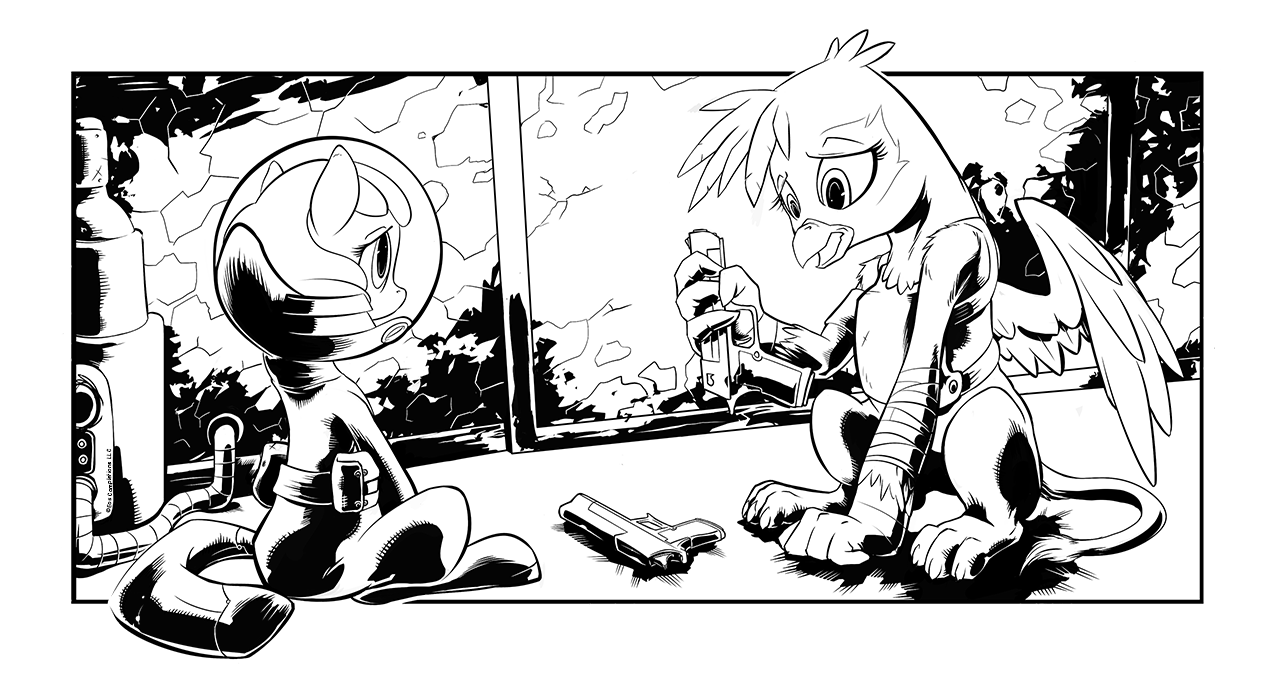
\includegraphics[width=0.9\linewidth]{image06.png}


\begin{intro}
    兰斯洛特,加拉哈德还有我一直等到日落,然后突然杀出去,
    
    把那些法兰西鬼子打得措手不及——他们甚至没来得及拿起武器!\footnote{这里是亚瑟王故事的节选}
\end{intro}

{\rt 晚上好,我最亲爱的听众们!你正在收听的是孤狼的52电台!这个频道有你们最想知道的52国道大新闻!}

然后是一阵班卓琴的短暂音乐声。

{\rt 让我们先从正事开始讲起,你们想要知道太阳是什么样子吗?问白苹果们吧!昨晚一个巨大的光球就在盐块城东边十公里左右的距离炸响了!很幸运的是,那里基本都是辐射蜥蜴和遗弃的窝棚。不过那光线就算在隧道镇甚至赤兔领土也能看得一清二楚。如果你觉得这件事非常疯狂,我要和你说,这个可是昨晚百老汇歌舞秀的一部分!首先我们看到一个载满尸鬼的气球升空——就是在盐块城圆顶肆虐的那些尸鬼!陪伴他们升空的是一个叫快乐帕比的小马表演的灯光秀,还真是个奇怪的名字,是吧,不过这个名字似乎听起来很耳熟吧?没错,她就是嘉年华的那位小幼驹!}

然后是一阵胜利的号角声。

{\rt 那么大家问我了,这新闻有什么意义?给那些『懒得听故事直接听结果的观众』一个简单版本!以后在盐块城郊外再也不会受到野生动物和尸鬼的袭击啦!}

然后喇叭里面传来一个拉枪栓的声音和一发枪响,然后还有一个非常硬汉的声音说:「{\rt 后会有期,丫头。}」

{\rt 我爱死这个小家伙了,两个城镇的问题被一个不会脱防辐射服的小幼驹解决了!就算我不是未卜先知,我也知道她一定会往南前进,那么……接下来是什么呢?她要重新开放隧道么?我说,孩子,如果你碰巧路过盐泥沼泽的荒芜之地,你一定要来看你的头号粉丝!我很想知道头盔里面的小脸有多么可爱!好了,现在和往常一样,来点超酷的音乐吧!}

\begin{music}
左一个小马,右一个小马

\begin{englishlyric}
    Here's a pony there's a pony
\end{englishlyric}

\medskip

还有一个小小小马,

\begin{englishlyric}
    and another little pony
\end{englishlyric}

\medskip

可爱的小马,快乐的小马,

\begin{englishlyric}
    funny pony party pony
\end{englishlyric}

\medskip

这就是小小小马!

\begin{englishlyric}
    pony pony sprite\dots
\end{englishlyric}
\end{music}

\horizonline

\daytimeplace{5}{16:45 PM}{165战指,盐泥沼泽}{165Th Brigade field Headquarter, Salt Marshes}

% TODO: 检查翻译

「关了那鬼音乐,老娘都听不到那死鬼是不是在外面了!」年轻的狮鹫怒气冲天地瞪了帕比一眼。

「但是……很好听啊!你真是个坏脾气小鸡!」小雌驹皱着眉头又抱她的萍琪派玩偶去了,「别担心丝尾,她没发火,只是累了。」

狮鹫赫瑞塔走到帕比身边,拎着她的头盔把她抓起来,好让她看着自己的双眼。「老娘最后一次警告你!是狮鹫!不是小鸡!外面老大一只蝎尾狮想把我们当晚餐,你丫还一个劲儿地找茬儿,是不是想死啊你?」少女的尖叫声又慢慢低了下去,「我真希望我老爸赶紧回来,」她叹了口气,「或许他能帮我逃出去,然后我就再也不用看你那张傻兮兮的脸了。」

「人家才不傻……你才是个坏心眼猫,我再也不想做你的朋友了!」

「{\mt 警告,检测到敌对狮鹫,距离3米,威胁等级:高。}」

「唉,别说啦,声音先生……」帕比做出一副夸张的厌恶表情转过身去。

「你让谁别说了?你和谁讲话呢?」狮鹫忽然睁大了眼睛。「你那东西还带无线电?」狮鹫跳到帕比背上用力想脱掉她的头盔。「我们可以呼叫支援啊!快叫我爸爸,他在 \SI{90.08}{Hz}!呼号炙红!」

幼驹被吓了一跳,「喂喂,等等!我要先问问声音先生!他住在这个防护服里面,操作那些奇怪的东西。」小雌驹举起蹄子嘘走赫瑞塔,不过狮鹫已经躲一边去了。

「等等,什么声音先生?这防护服能说话?」

「当然可以!这是最好的太空服!而且它超级聪明!」帕比自豪地笑着。

「对哦……」赫瑞塔嗤之以鼻,「比你聪明多了。」

「当然,比我聪……」小雌驹的笑容变成怒容。「喂喂!怎么能这么说人家!」

狮鹫被她逗乐了,「你丫这么简单的招都会中么,你这小鬼太搞笑了,自己承认自己比个香蕉睡衣都蠢!」赫瑞塔说着用爪子弹了一下小雌驹。

「喂喂喂!干什么呢!坏心眼小鸡!如果不是你爹地伤得那么重,我早就教训你了哦!」

赫瑞塔一下愣住了,盯着帕比问:「我老爸怎么了?你怎么认识我老爸?」

帕比看着少女充满希望和惊恐的表情,觉得自己应该非常非常非常谨慎地选择自己下一句话。

「呃……上次我见他的时候,他状态是……死亡,或许他现在已经好点儿了?」幼驹满怀稚气和天真地微笑着。

「我……老爸……死了?你怎么知道的?你什么时候看见他的?这不……这不可能!他是最棒的!不可能死的!你绝对看错了!快跟我说这不是真的!」狮鹫拔出她的白色手枪,带着黄色条纹的枪口指着幼驹的鼻尖。「快说!你看错了!」

赫瑞塔发红的眼睛死盯着帕比粉红的眸子——幼驹虽然有点结巴,但是那双闪闪发光的粉色双眸绝对不可能撒谎,她只是一个稚气未脱的小孩子。

「我……我不知道,他……只是跟我说……他想和你说,他非常非常非常想和你在一起,他很抱歉,所以我超级快地跑过来找你,因为我觉得他看起来伤得很重,而且我很想我妈妈……」

「住口!」赫瑞塔一爪子把帕比拍飞到了墙上,跪在地上把头深深埋在双臂之间,不敢面对残酷的现实。「这不是……这不是真的……我爸爸……是最厉害的赏金猎人……他绝对没事的,他一定会赶来救我……我……我……」

一个金属碰撞的铿锵声让少女抬起了头。

帕比站在赫瑞塔面前,幼驹什么也没说,只是把那柄带着红色条纹的黑色手枪放在狮鹫面前,然后又蜷缩回房间的角落。

「黑玫瑰……」年轻的飞行员吃惊地瞪大眼睛看着面前的枪。「不……不……不会……不可能的……这不是……」她又一次看着穿黄衣的小马。「拜托……求你告诉我……这不是真的!我只是在做噩梦!」

帕比皱着眉头低下了头,「我……我不知道……如果这是一个噩梦的话,那我醒来的时候,妈咪一定会在我身边安慰着我,所以……我希望这也只是一个长长的噩梦……」幼驹又叹了口气,「但是,我不觉得这是……」

「肏!」赫瑞塔用爪子抓起那个手枪,和她自己的点45手枪完全一模一样,除了颜色。「到底发生了什么?为什么你会在现场?」\thpr{冷静点儿,赫瑞塔,别情绪化了,你应该问清楚她情况,你可以做得更好,你必须做得更好!}

% NOTE: . -> 点

「我看到天上好像有四个小鸡……」

「不!准!叫!老!娘!小!鸡!我们是狮鹫!比你们这些蠢小马厉害几百倍!你要再叫老娘一次小鸡,那就是你丫这辈子的最后一句话了!懂不懂?」狮鹫拎着帕比的脖子,另一只爪子举着枪顶着她大吼道。

幼驹的眼睛充满了恐惧,她挣扎了两下想要逃跑,但是很快就放弃了,她大哭起来。「我……我很抱歉狮鹫小姐!我会乖乖的!别……别欺负我……」

赫瑞塔点点头把她放下来,「这下好多了,有四个狮鹫在天上飞,然后呢?」刚才的怒气似乎冲散了狮鹫的其它情绪,让她可以更认真地听帕比讲下去。

快乐帕比结结巴巴地继续她的故事,不想让可怕的狮鹫再发火。「就是刚刚,我和朋友正顺着路走,然后天上……呃……天上……开始好像是他们在跳舞一样但是他们看起来好多受伤掉了下来我走过去看他们最后掉下来的一个跟我说给你那个黑东西然后和你说他很抱歉他想往南去我戳戳他想让他醒来但是他还是一直睡我真的真的真的很努力去戳他让他醒来但是他就是不醒来!请别对我发火我真的真的真的想让他好起来但是声音先生和我说他已经『死亡了』而且……而且……」幼驹后退了几步,缩成一团,用前蹄抱着头盔。「请不要欺负我,我真的没有恶意,我只想帮忙!对不起!」

\thpr{肏,算了,她只是个孩子!}狮鹫摇了摇头,自己的怒火也开始消退,这个幼驹估计都不知道『小鸡』对狮鹫而言是侮辱性的称呼……趁她还没给自己惹上真正的麻烦之前,某狮鹫还是好好教她吧。

「那个某狮鹫还能是谁?」赫瑞塔长叹一口气,轻轻拍着帕比的头盔,「好了没事了,真的,叫我赫瑞塔,或者赫瑞好么?你只是有点……没教养,别担心,我教你就是。现在我们还是想个办法出去吧。」

「但是……你刚刚还对我发火……」帕比还是双蹄抱头的蹲防姿势。

「我没生气,真的……做个好孩子,站起来,好不好?」

「但是我叫你小鸡还说你是坏蛋……」幼驹小心地露出脸。

「别那么叫了行不行?我也对你吼过了,我们扯平了,可以吧?」

「所以……所以我们还能做朋友?」帕比满怀希望地问。

狮鹫叹了口气,「对,我们还是朋友……现在让我安静一会儿,我好想个办法出来。」

对,办法,说起来简单做起来……好吧,不是一般的难,但是至少这些话还是让帕比再次变回了快乐模式。幼驹点了点头坐在楼梯上,狮鹫看着外面,那猎食者估计在哪里躲着,等她们自己走到空旷地去。

「没戏……要是我有比枪更厉害点的东西,或许还能拼一下,不过如果……」狮鹫回头看着帕比,「我说,你不会刚好带着爆炸物或者重武器吧?」

「我有一个石头!超耐磨!」帕比自豪地把「命运之石」展示给赫瑞塔看。

狮鹫不屑地嗤之以鼻,「还真是CNM!抱歉,我可不想把我的命赌在这块蠢石头上。」

雌驹歪着她的头,一脸不解地看着她最喜欢的武器。「小石石,我才不觉得你蠢……不过现在你还是回包包里睡觉吧。」

「拜托!老娘正在想个正儿八经的主意呢!别在这儿和你包包里面的东西挨个吻别了,你他喵的能做点有用的么……比如……比如说……算了,你还是去和你的闪尾玩去吧。」

「丝尾!」

「对,就是那玩意……一边玩去……」

「好的好滴好的!茶点五分钟就来!」帕比坐在楼梯上开始和她的萍琪派娃娃聊天。

「无论如何……」狮鹫开始低声自言自语,「附近没有任何掩体,我估计只能带着那东西跑个几分钟,好吧,我们真的需要重火力……」赫瑞塔无奈的叹着气,「简直太扯了,外面的坦克装满各种炮弹,我们蹲在这里,只有三把点45手枪和一个……石头……」

% NOTE: . -> 点

这个时候,帕比正在把她的玩偶放在一枚大号坦克炮弹弹头上,然后用另一个当做茶壶来沏茶。「喏,你杯子里面要6块还是8块方糖?呃……你有杯子么?」

「不,谢了,我不要,我想我有个办法了。」狮鹫完全懒得去看幼驹在做什么,她一边继续观察着外面一边说:「我先跑出去吸引那蝎尾狮的注意,等他开始追我的时候,你冲到最近的坦克里面,你最好快点,因为我不能带他跑太久,你要找的是高爆弹头,那东西又大又亮,像一个尖头大水壶,而且上面有个红条,懂了么?」

「呃……好吧……」帕比看了看她蹄子上的『水壶』然后耸了耸肩把那东西放一边,「那你能帮我看好丝尾么?」

「我觉得我们出去之后你的玩偶也不会跑哪儿去的,你丫就给老娘利索点儿,去坦克里面拿个有红头的大『茶壶』回来,等你搞定这事儿之后我们再继续下一步计划。」狮鹫蹲下来,活动一下筋骨准备冲出去,她现在需要自己是最佳状态。

「但是……她会害怕!」幼驹继续冒着傻气。

「帕比,闪尾只是个玩偶!她不可能害怕!」赫瑞塔扭头抓起那个萍琪派玩偶,在幼驹面前晃着说:「看到没?她在笑!她没关系的!回来时候说不定她还能给我们办个……高爆弹?」狮鹫瞪大眼睛看着帕比玩具的那个椅子。「呃……你从哪儿找到这个的?」

黄衣幼驹开心地说:「炫彩大厅!软气给我的!」

「不是……我是说这个椅子……」

「哦,这个啊……在那个坏掉的大铁马车里面,闪闪发光哦,我拿了好几个。」看着狮鹫的表情,帕比于是又说:「你想要吗?」

赫瑞塔眼角抽搐着,「这……真好……第一步完成了……现在我们开始第二步……」

「但是我们什么都……」

「好了,啥都别说……我们,第二步,懂了吗?」狮鹫觉得自己的自控能力越来越好了。「你仔细听好,我把那个大坏蛋引到这个塔的门口,当那蝎尾狮探头进来的时候,你就把这个弹头丢进他嘴里,然后我就打爆他,然后乒,炸飞他的头,然后坏蛋就死翘翘了!」

帕比皱了皱眉头,「就是说……我把茶壶丢进他嘴里然后电影就结束了?」

「电影啥?哦对,把那东西丢进蝎尾狮嘴里,然后我处理剩下的事,好了,你准备好,别吓坏了,懂?」

「好的好的……」幼驹抱起弹头然后躲在墙后面,赫瑞塔谨慎地展开翅膀探出头。

不过一分钟,外面就传来枪声,还有一大堆帕比完全没有听过的精彩狮鹫方言骂街,幼驹超超超好奇外面到底发生了什么,但是赫瑞塔叫她乖乖呆好。现在幼驹觉得有点麻烦了——如果赫瑞塔发现她溜出去了那么一定会很生气,她生气起来可害怕了……但是帕比觉得外面一定有什么超级酷的事情发生,而且生怕错过了。

「或许稍微稍微稍微看一下下……」听着外面的怒吼声和枪声,幼驹抱着她的高爆弹,小心地爬到了门口。「就看一下下……一下下……绝对没关系的。」

「哎,啥都看不见!这不公平……」

忽然一个残影飞快地冲过门口跑到房间的对面大叫着。「就是现在!」

「现在啥?」帕比有点奇怪地问。

嗷呜!!!

随着一阵水泥碎块飞溅,蝎尾狮脑袋冲进门来,但是身体却卡在门框上进不来,帕比发现自己就距离那巨兽的尖牙只有几厘米的距离,让她吓得尖叫一声坐了一个屁股蹲。

「你丫搞什么呢!快丢那劳什子然后趴下!」赫瑞塔惊恐的大叫起来,「给老娘动起来!」

黄色幼驹大叫一声发射了炮弹——那弹头画了一个小小的抛物线,而帕比则以一个更大的抛物线向后蹦了出去,在弹头落在野兽面前的时候,狮鹫举起了枪。

乒!乒!乒!

% NOTE: 呯 -> 乒

三发射击,三发命中,三发跳弹。

「肏!谁尼玛把弹壳做这么厚枪都打不穿!」

双枪少女一边骂着一边把手枪里面的所有子弹都倾泻在那个破弹头上,但是却什么都没发生。

「肏,肏,肏,没用!」赫瑞塔收起双枪然后拿出第三把手枪,那把黑色并且有着红色条纹的手枪——这把枪和她的另外两把没什么区别,她把一梭子子弹打在蝎尾狮鼻子上,终于让那个怪物退缩了一下。

「我想他正在把入口弄大。」帕比又后退了几步,而且看起来没那么害怕了,幼驹轻轻敲着自己头盔下巴的位置,看起来好像在分析战局。「他好厉害哦!」

野兽血红的双眼瞪着赫瑞塔,显然他不打算再回外面蹲伏去了——即使这意味着他要把整个指挥塔拆掉来抓狮鹫,而且他也正在拆了,虽然拆得有点慢。

「在那傻站着干啥,赶紧滚过来!」狮鹫一边给手枪装子弹一边吼着。「就算老娘手枪打不响,但是如果打中引信还是能把你的屁股炸开花,你丫给我找个掩体蹲好!」

「吟新……是啥?」

赫瑞塔忽略帕比的又一个傻问题,从掩体跳出来,双枪瞄准那个炮弹的引信,「说拜拜吧,你这个……」

就在这时,年轻的飞行家注意到蝎尾狮正在低着头弓着身子做出飞扑准备动作,等赫瑞塔飞到空中的时候才知道蝎尾狮的弹跳能力有多好,但是已经太迟了——她连骂街的机会都没有,一瞬间就被蝎尾狮的爪子像拍苍蝇一般从天上拍了下来。

赫瑞塔被蝎尾狮有力的爪子按住了肩膀,她无助地挣扎着,被蝎尾狮撕扯着。

快乐帕比也同样惊恐地尖叫起来,幼驹想后退,但是自己的臀部已经碰到了墙壁,蝎尾狮非常非常可怕,它正在伤害赫瑞!

那一瞬间,帕比看到的不是蝎尾狮,而是一张双眼闪着光的粉红色金属面具。

「\rcpr{求你……哈哈哈……别让我……哈哈哈……笑了……\footnote{嘉年华的瑞吉}}」

帕比双眸之中点燃了粉色的火焰,她举起蹄子大喊:「石头!」

「命运之石」立刻飞到她的蹄子上,幼驹高高跃起冲向那个野兽。

「放开她!快放开她!」

蝎尾狮被黄色的小小奇袭打乱了节奏,他把自己的旧猎物丢到了一边,怒吼着转向小小幼驹。然后张开血盆大口,随着清脆的咔嚓一声,黄色的小雌驹消失在怪物嘴中。

赫瑞塔尽力保持自己的清醒,挣扎着爬上楼梯,而那头蝎尾狮得意地吼叫声为帕比的命运盖棺定论。

「不……不,已经太迟了……快逃命吧……别回头看……」重伤的狮鹫一边自言自语,一边爬上楼梯,只是走这几步身上的伤口就让她痛得快昏过去了,身后蝎尾狮正在疯狂地怒吼着,估计正在撕扯那可怜小家伙的尸体,赫瑞塔拿出一瓶治疗药水一饮而尽,然后转头看着楼梯下面。但是她只能看到一片粉红色的烟雾,接下来伤口的剧痛和失血让她失去了意识。

……

现在,还是让我们为那个非常不走运的蝎尾狮默哀一分钟吧。

这就是为什么说『绝对不要随便乱吃东西』,因为那肉显然已经变质了。

\horizonline

\daytimeplace{6}{00:45 AM}{165战指,盐泥沼泽}{165Th Brigade field Headquarter, Salt Marshes}

「{\mt 系统重启完毕,所有功能恢复,自检系统上线,目标001:快乐帕比,雌性陆马,目标已死亡,体征状况稳定,完毕!}」

懒洋洋地睁开眼睛,帕比打了个哈欠。「外面还黑洞洞的呢……」睡觉的时候还被什么重物压着,这让她很不开心。

「发生什么事情了?小鸡呢?大坏猫呢?」

「{\mt 分析中,监测到敌对生物,距离6米,赫瑞塔,威胁等级:可忽略。}」

一个红点在罗盘上闪烁着。

「傻声音,赫瑞不是敌对圣姑!」

那个红点变成了粉色。

「很好,我们出……咦?」蹬着蹄子却发现自己没在移动,帕比这才注意到她挂在灰白色的杆子上。花了吃奶的力气,帕比好不容易从蝎尾狮的骨头堆里面钻了出来,那个野兽的骨架看起来已经和墙壁的颜色一样,似乎已经和墙壁融为一体,而那个长满利齿的白色骷髅头仿佛正在绝望地嚎叫,翅膀的骨头也伸开,似乎它不顾一切想要逃开那吞噬它的致命粉云。

帕比走到了赫瑞塔身边,但是狮鹫却一动不动地躺在地上。

「声音先生……她是不是……你知道的那个……死了?」

「{\mt 分析中,否定,目标失去意识。}」

「哦……这表示她会好起来?」

「{\mt 肯定,目标恢复中。}」

「好滴!」这句话对于帕比来说就够了,她开心地隔着头盔和赫瑞塔吻别。

「我很抱歉,但是我必须走了,小鸡,我妈妈还在粉箭头的末端呢!」

帕比走了几步,但是又退了回来。她觉得只是吻别似乎不够,幼驹拿出萍琪派玩偶然后放在狮鹫的爪子中。

「听好,丝尾,帮我照顾赫瑞塔,别让坏事发生在她身上。」

这次没什么问题了,帕比开心地跑到外面,然后捡起自己的滑板车。

「嘿,能来点音乐吗?」

\begin{music}
在丛林中,密密的丛林中。

\begin{englishlyric}
    In the jungle, the mighty jungle,
\end{englishlyric}

\medskip

今晚狮子在沉睡。

\begin{englishlyric}
    the lion sleeps tonight!
\end{englishlyric}

\medskip

在丛林中,恬静的丛林中。

\begin{englishlyric}
    In the jungle, the quiet jungle,
\end{englishlyric}

\medskip

今晚狮子在沉睡。

\begin{englishlyric}
    the lion sleeps tonight\dots
\end{englishlyric}
\end{music}

\horizonline

\daytimeplace{6}{10:00 AM}{狮鹫陨落之地,盐泥沼泽}{Griffon's Fall, Salt Marshes}

不用铲子挖坑本身就是一种折磨,而在泥泞之中,用你自己的爪子挖自己父亲的墓穴,简直就是……

大颗的泪水顺着狮鹫的喙滑落,每一次她想要挖出泥土,就会有更多的泥水落回来。但是她却无言地继续挖着,他从来没让她哭过,他是最厉害的最顶尖的佣兵,但是现在他死了,被鹰爪佣兵\footnote{鹰爪佣兵(Talons):狮鹫公国被英克雷吞并之后,流亡的狮鹫组成的大型佣兵组织,大多数狮鹫都属于鹰爪佣兵}杀害了。

赫瑞塔把他拖进浅浅的墓穴里面,尸体在泥泞之中发出湿软的声音,女儿看着自己父亲的鲜血渐渐渗入泥土之中,努力把自己的泪水咽下去。

他喵的……这个墓穴甚至不能装下他。

「这不公平,把我自己孤零零地丢在这里……我现在还能去哪儿?」赫瑞塔叹息着,她想要发火,但是却一点怒气都没有。他已经走了……还能怎样。

「为什么……」

肏!

肏蛋!

狮鹫慢慢地用泥土和附近的碎石将墓穴盖好。她拿出黑色的手枪,迟疑了一下又放了回去,然后拔下自己的三根羽毛,然后放在她父亲永远安眠的胸口附近。

「跟老妈说我会照顾好自己的,明白吗?」

赫瑞塔揉了揉眼睛,然后拿起她的包,看着包里面漏出来的丝尾,凝望着那玩偶的蓝色双眸,她再一次露出了笑容。

「我会照顾好自己的。」

\horizonline

\daytimeplace{6}{11:30 AM}{随机遭遇地点,盐泥沼泽}{Random encounter location, Salt Marshes}

「嗨!我叫快乐帕比!」

三个奴隶贩子当中的黑色陆马皱了皱眉头,「我想我听过这个名字……或许我们还是别……」他看了看另外俩伙伴——他们都和他一样武装到牙齿。但是前两天他们都听过孤狼说到的游荡在52号国道北边的幽灵。

「我才不怕幽灵,血滴,如果一个幼驹就能把你吓出翔来,那你就滚边一去!」看起来是奴隶贩子头头的黄色独角兽打量了一下他自己的『货物』,两只公马和一只年轻雌驹……完全不如往常的多,「四十钉,抓住她!」

快乐帕比有点迷糊,在罗盘上有六个点,三个是粉色,另外三个是红色……声音先生总是搞奇怪的东西出来,一个红点的小马靠近她,然后小心地把蹄子放在她背后。

「小子,跟我们走,别反抗!」

「好的,好得!我们去哪?」黄色的幼驹一脸兴奋。

对于新奴隶而言,她的举动很明显非常奇怪。她身边那只小马,绿色的独角兽看了看他老大,而后者耸了耸肩,「看到了么,这就是被卖了还帮着数钱的典型,给她带个项圈。」

四十钉想要剥开帕比的外衣,但是他显然不是和平部的技师。

「我说,老大,这破玩意弄不开!」

「呃……我也脱不下来,这个头盔粘得厉害……我还试过打碎它,但是它不停地自动修复!」终于有小马帮帕比解决太空服问题了,不过他们看起来完全没有足够的知识和技巧。「我想或许会有个开关啥的,但是每个开关都没用!」

「闭嘴,白痴!」四十钉显然没有耐心了,所以他还是用最原始的办法解决问题。他举起一把超大号扳手然后砸在帕比的头盔上,把头盔表面砸出蜘蛛网一样的裂痕。

黄色独角兽咆哮起来,「你丫要敢砸碎她脑袋,老子就把你的脑袋也捎带上!死幼驹一文不值!」而那个黑色的奴隶贩子看着另外三个奴隶,对这一幕喜剧窃笑着。

帕比害怕地后退一步。

「我说,这太危险了吧!」

「{\mt 警告,罗盘失灵。警告,感应器离线。警告,头盔受到破坏,修复中。}」

「卧槽他喵的,这蛋壳还真结实!」绿色独角兽再一次举起扳手的时候,看到那个裂痕已经完全消失了。「我勒个去!」

「用个绳子给她捆起来然后赶紧走,等我们从这个屎坑出去之后再处理那问题。」

他们叫帕比乖乖地,于是帕比就乖乖地看着漂漂小马给她脖子上套了一个绳圈,他们把她和其他奴隶一起拽着走的时候,帕比觉得有点不对劲。

「喂喂,我不能把我的车子丢那里啊!」幼驹走向她的滑板车,但是那个奴隶贩子把她扯了回来。

「你丫想去哪?」

帕比挣扎着说:「我的滑板车!放开我!」

四十钉冷笑了一声,「没错,小婊子,」他把小雌驹扯到面前,看着她的眼睛说。「你现在是奴隶了,把你的滑板车和别的什么东西都忘掉,如果你还想活命就给我乖乖地,听明白了么?」

「但是……我要去那边!」帕比用蹄子指着南边。

绿色的独角兽啐了一口然后用他的枪柄打着幼驹的屁股说:「给老子闭嘴,竖起耳朵听好,要不然肏爆你这个小婊子的屁股!反正不听话的小马卖不了好价钱!」四十钉转头对奴隶主说:「喂,老大,我要给这小婊子上一堂礼仪课!」

「别把她玩坏了,不然你要掏她的钱。」领头的头都懒得回,继续往前走。

黄色的幼驹皱着眉头。「先生你不可以说脏话……」她的表情看起来好像绿色奴隶贩子刚刚打她的那一下完全不疼不痒。

「闭嘴!」

帕比被打得飞了出去,摔出几米远,「喂喂,别这样粗鲁,会有马受伤的!」她一脸完全没事的样子站起来,反而有些担心地看着四十钉。

「怎……怎么回事……你是啥玩意?滚远点,别动!」奴隶贩子举起枪瞄准幼驹。

乒!乒!

% NOTE: 呯 -> 乒

两发子弹在幼驹胸口打出两个洞,但是她完全没有反应,四十钉惊恐地瞪大眼睛,这个时候奴隶主回头怒视着他的走狗。

「肏你娘的龟孙子!你丫吃错药了么?这是你最后一次杀我的奴隶!」黄色独角兽低头冲向绿色小马,把他撞飞到一边。

「不……我……我才不要死在这里!」四十钉一脸惊恐转头把弹夹里面的剩下子弹射向他的老大,那个奴隶贩子头头还没反应过来发生了什么膝盖就被打碎了。跪在地上的独角兽拿出他的突击步枪开始乱扫起来,黑色的陆马也拿出一把散弹枪,乱飞的子弹又在帕比身上打了一个洞,但是看起来完全没有影响到幼驹。

「别吵架啊,喂喂!我说!你也是!」帕比想要恢复一些秩序,但是显然事态已经超出她的蹄下。

「你们都是大坏蛋,你们不觉得害臊么?声音先生,做点什么啊!」

「{\mt 修理完成,气密性恢复,目标001:快乐帕比,已经死亡,体征正常,完毕!}」

「不是这个『什么』,是做点别的『什么』!」

黑色的奴隶贩子掏出一瓶治疗药水刚想要喝下去,他的枪就被另一个公马奴隶夺了过去,然后那张丑脸就被一发散弹打得四分五裂。俩受伤的独角兽倒在血泊之中对射的时候,那个怀孕的雌驹正拼命地想在这个尸体背后寻找掩蔽。

四十钉比起他流了一大滩血的奴隶主还多了一口气,不过他不想独自下地狱,随着他的角发出光芒,所有奴隶项圈上炸弹的遥控器从他背包里面飘了出来。他躺在地上一边咳血一边露出狰狞的笑容,「别害怕……咳咳……小马们……咳咳……你们……会先……咳咳……死!」他举起他完好的蹄子慢慢伸向开关,两个还活着的奴隶惊恐万状地看着他。

「没收!」一个黄色的蹄子从他面前把引爆器夺走了,「坏小马不能玩玩具!」帕比用她最认真的表情看着他。「我说了别发疯!在你乖乖坐好之前这个由我保管!」小雌驹一脸严肃地说:「我说到做到!」

奴隶贩子看了看帕比,然后仰天长叹,「我……真难以置信……我……咳咳……一直听……咳咳……幽灵的故事,」他的眼睛看着帕比防护服上的最后一道划痕消失,「你丫……咳咳……比我想得……咳咳……还要可怕……一万……」他的声音和生命一起被饥渴的废土吞噬了。

\horizonline

\daytimeplace{6}{8:30 PM}{隧道镇外,52号国道北口}{Tunnel Town Outskirts, Big 52 N Branch}

「当小马妈妈和小马爸爸超喜欢对方的时候,他们就写信给塞拉斯蒂娅公主要一个小幼驹,你们真的不知道吗?」帕比一边在附近蹦来蹦去一边说。

在盐泥沼泽冗长但是又幸运的散步之后,那无穷无尽的泥坑终于抛在他们身后,路面变成了崎岖的山路,随着夜幕降临,远处的景色渐渐模糊,夜间的掠食者也出来活动,帕比的HUD上闪烁着野生动物的红点,但是它们基本是被她的超自然力量惊得四处逃窜。

那对和快乐帕比一起走的小马也一样苦不堪言,那个叫甜花的奶白色怀孕雌驹先开口了:「差不多……呃……大概就是这样……你真的挺能说的。」

「没错!大家都这么说!」帕比微笑着继续说:「我希望你能有一个小雌驹,小雌驹超可爱!」然后她压低声音说:「而且,我听说男孩子身上都长虱子,不骗你!」

甜花咯咯笑着,轻轻蹭着她的伙伴,那个叫阿索的棕色陆马。「她这一点没错,是吧?」

阿索笑了笑:「那景色看起来非常壮丽吧!」公马停了下来看着远方。「我们到了,小家伙,这就是大隧道。」阿索用蹄子指着山崖边上的灯光说。

一座用石头搭成的巨大拱桥穿过泥潭,直接爬上山崖,就像是通向天空的大道一样。帕比瞪大双眼看着这壮丽的大桥,就像是大陆直接射向山崖,然后,乒——炸成了一堆五颜六色的灯光。不过她的两个伙伴似乎对她更感兴趣,因为幼驹双眸射出的粉色的光芒穿直切切穿过黑暗,而在她头盔上也漂浮着一圈淡淡的鬼火。

「好滴!那么,我们现在就去那边么!妈妈在那里等我呢!」帕比兴奋地问着,完全没注意到那两个小马在相互使眼色。

「呃……不过……我们不住在那里……而且你进隧道镇还要交税,我们去荒芜之地的贸易站,那里稍微远一点。」阿索有些迟疑,但是雌驹蹭了蹭他,鼓励他说出他们的想法,在顿了顿之后,公马低下头继续说。「我……我们想知道:你真的是个幽灵?还是上天派下来保护孩子的守护天使?」

帕比歪着头,然后咯咯笑起来,「我是快乐帕比,漂漂笨马!我不知道为啥大家都叫我幽灵,我只是在找我妈妈!」

「对……你和我们说了上千次了……」阿索耸了耸肩看着他的伴侣,「那么,我想就这样了……毕竟我们欠你……那么……可以接受我们只是说『谢谢』么?我真的很想用什么东西报答你,但是我们在活着回家之前真的什么都没有。」

「好的好滴好得!拜拜漂漂马!」帕比注视着她的新朋友消失在夜色中,然后顺着桥走向隧道镇。

~\vfill

\begin{note}
    升级(Lv 5)

    新技能解锁:快速训练:力量($5 \to 6$)你现在能在包包里面塞好多好东西了!
\end{note}




\chapter{临时保姆}

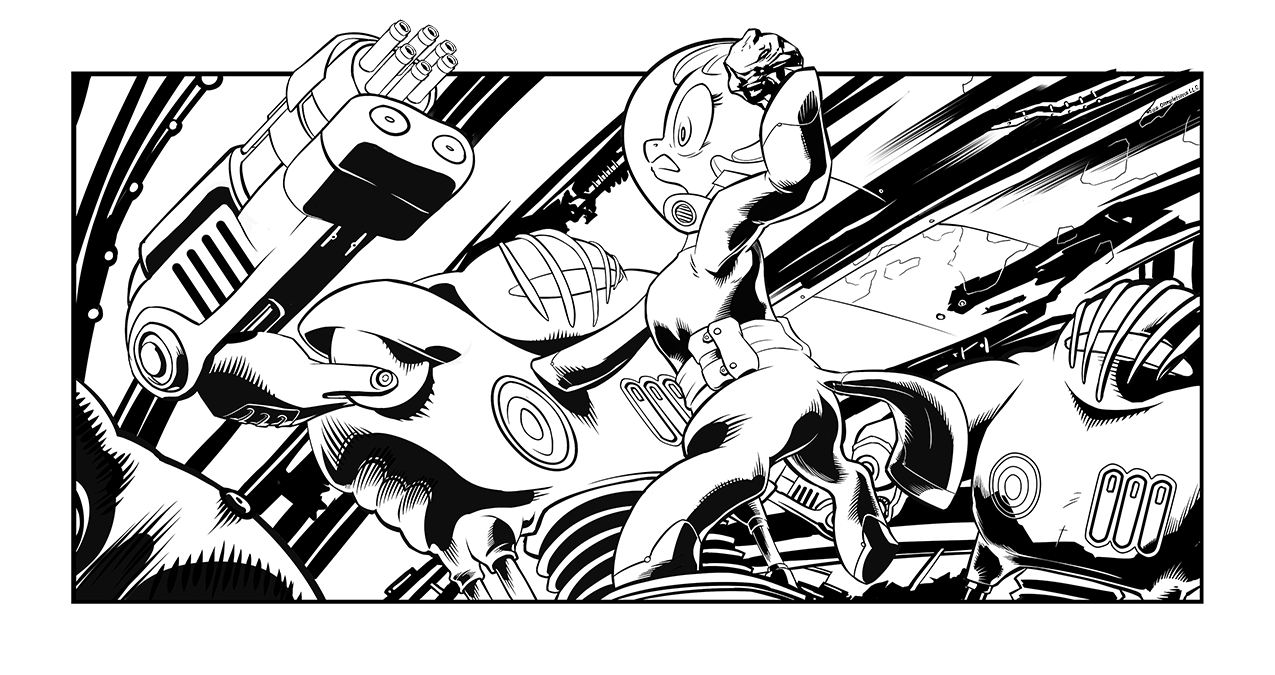
\includegraphics[width=0.9\linewidth]{image07.png}


\begin{intro}
    什么?你说那些可爱的小天使?照顾他们完全没有问题!
\end{intro}

\daytimeplace{6}{9:00 PM}{隧道镇,52号国道北口}{Tunnel Town, Big 52 N Branch}

快乐扳机(Trigger Happy)已经当了半辈子卫兵,她很确定自己见过各种各样想要进隧道镇大门的家伙。不过她现在觉得自己见识还是不够。现在她所有的卫兵同僚都战战兢兢地缩在她背后——只是因为那只穿着滑稽的幼驹现在看起来更不开心了。

「唉,你们这些胆小鬼,算了交给我来吧,你们放松点儿。还有看在我尾鬃的份儿上,别乱开枪。」

独角兽雌驹走出那群卫兵,朝那只被粉色鬼火环绕的黄色小幼驹走去。

「你,就站那儿!别再靠近了,告诉我你到底是谁?」

扳机并没有期待那只幼驹乖乖听话,不过看着她坐下,守卫队长还是松了一口气。

奇怪的孩子挥着一只蹄子向她打招呼:「嗨!我叫快乐帕比!你看到我妈妈了吗?」

扳机皱了皱眉头,「快乐帕比……你就是那个小幽灵帕比?」

「我不是幽灵,我只是个小雌驹!」幼驹嘟起了嘴,她背后还背着一个长长的红色滑板车,看起来不像是武器,虽然的确很大。

「你想说,你就靠一个红板\footnote{红板(Red Racer):飞板璐长大之后开办的玩具公司销售的主打产品,速度非常快的滑板车,虽然对小孩子略有些危险,后来小璐靠卖这个赚的钱和其他CMC一起成立了避难厩科技。}一路从盐块城穿过盐泥沼泽跑到这里?」

帕比咯咯笑起来,「才不是,胖胖独角兽走得超级慢,所以我也得慢慢走。」

「谁谁谁?算了,别提这个了。」扳机叹息着,「我要过去了,你别做……呃……那些鬼鬼怪怪的事情。」

她回头看了一眼,正好和掩体后面露出的三对惊恐的眼睛对上,其中之一还举着一面小白旗晃了晃。她真心向女神祷告,祈求能有几个更靠谱的队友。然后她走向帕比。

「嗨!你好漂亮!漂漂小马姐姐!你叫什么名字?」幼驹露出她最友善的笑容。

\thpr{她只是……只是……只是一个有对发光双眸的幼驹而已,估计只是受了点辐射影响。}「没搞错吧,你就是新闻说的那个快乐帕比?那个来自盐块城和嘉年华的幽灵?」卫兵笑了起来,「拜托,别扯了!」

帕比也跟着笑了起来,「哈哈哈!很有趣对吧!呃……不过哪里有趣了?」

幼驹的问题让卫兵队长笑得更响了,「快乐扳机,但你叫我扳机就好。」

帕比皱了皱眉头,「啊,我能叫您乐乐么?」

「当然,对了,我还有个东西……」扳机拿出一片黄色的塑料卡递给帕比,「这是你的通行证,中午有个叫赫瑞塔的狮鹫来到这里,她一直等你到傍晚,但是你还没来,所以她先走了,不过她走的时候还帮你交了通行费,她说你最迟明天就会来。」

「呃,赫瑞在这里?她还好么?」

「我想……她很好,不过她不太爱说话,不过我也没碰到过爱说话的狮鹫。」扳机扭头往回走。「进来吧,在外面可不利于健康,附近可有不少血翼\footnote{血翼(Bloodwing):吸血果蝠受辐射影响以后,真的吸血了}。」

「血翼是什么啊?」帕比跟在扳机背后问。

「如果你问我的话,他们就是麻烦!是长翅膀的大号水蛭!」雌驹笑着伸蹄子招呼帕比走进去。里面是一间用沙包和生锈的铁板围成的简易窝棚,两挺加特林机枪在窗口前指着桥头,而墙角堆着一大堆弹药箱——还有三只全身紧绷的小马一脸尴尬地打着招呼。

「伙计们,别这样。这是快乐帕比,嘉年华的小英雄,她和我们可是一伙儿的,所以别害怕好吗?」卫队长举起蹄子掩嘴窃笑,「我还真想看看孤狼亲眼看到他所说的『英雄』是什么样子会有什么反应。哦,这几位是绿梨,坏枪和小豆子。」

「嗨!我叫快乐帕比!」幼驹蹦跶到仨小马面前。看着她的新朋友们一脸紧张的表情,于是她又接着说:「我正在找我妈妈!她或许会在山里面!」

三个守卫之一低声嘟囔着:「这下麻烦可大了……」

\horizonline

\daytimeplace{6}{9:45 PM}{隧道镇,52号国道北口}{Tunnel Town, Big 52 N Branch}

「哇塞!好大哦!」帕比看着隧道入口,一直仰头到一屁股坐在了地上。这个隧道大到可以同时让天空马车和普通马车一起出入,而且有两排车道!隧道的混凝土墙壁在深入山脉20米之后,被一道生锈的巨大铁门硬生生地截断了,那面铁门上是一个白色的天角兽标志,看起来那标志简直比女神更雄壮威武。标志下面是一行字:旭日公司——走可持续发展道路,而字下面,又是一个平常门上都会有的大大危险警告标志。

「看到了吧。」扳机敲了敲那个金属大门,「它封死了,我很抱歉,小家伙,但是这估计就是你旅程的终点了。」

「但是……妈咪在里面!你看那个箭头!它指着大门呢!我得进山里面去!请打开它,拜托!」帕比闪着水汪汪的大眼睛。「超超拜托,漂漂的乐乐姐姐!」

卫兵队长后退了一步,「哎呦,这眼睛绝对该列为违禁武器……不过,我很抱歉帕比,就连我们自己也没办法进去。为了打开它,我们都不知道试了多少次了,不信你看吧,我们现在还是零分。」

「但是我真的,真的,真的真的真的要进去!妈妈在里面等我!」小雌驹满地打滚。

坏枪摩挲着自己的胡茬子,低声地自言自语:「我想那个TNT曾经说过可以从通风管进去?」

扳机瞪了他一眼,「闭嘴!」然后转头满脸堆笑的看着帕比。

「懂了么,没办法进去!」她想板起脸,但是小雌驹早已经不吃那套。

「呃,洞风道?那是啥?拜托,告诉我!我为你做什么都行!哦哦哦,我拿这个跟你换!」帕比忽然掏出一个从军事基地拿出来的坦克炮弹头,这一个上面是黑带,「你看,这个闪闪发光的东西超级厉害!您让我进去我就给你这个!成交么?」

「帕比……这危险了!我不想让幼驹去送死,抱歉。」

幼驹后退一步,看起来她就快要哭出来了。「我才不怕!这不公平!如果你们妈妈被关在里面你们肯定早就打开这破门了!而且……而且……」小雌驹尥蹶子踢着门。「我不能在这里放弃,她在里面!她一定在里面!」

坏枪趴在扳机身边耳语着:「为什么不让她进去,她已经救了俩城市了……我可不觉得她只是个一般孩子。」

独角兽卫兵叹了口气回答:「我们现在根本不知道隧道里面有什么,你好好想想大门关上的那天,我可以清楚地听见困在里面的小马敲门呼救的声音,还有枪声和惊恐的尖叫。」扳机用蹄子敲着坏枪的前额,「你好好看她,就算她也许是个不一般的小家伙,不过她也只是个孩子!我绝对不会送个孩子去踩雷区!」

公马卫兵注视着他上司的眼睛,「你觉得她会就这么放弃?如果她真的是那个幽灵,那我觉得我们也没什么办法阻止她。」

快乐扳机以蹄扶额摇着头,「你还真信那些床边故事?拜托,醒醒吧,她就只是个穿着全套防辐射服还稍微受了点儿辐射影响的小孩子而已!」

这个时候帕比依然站在大门前垂头丧气,「我不是小孩子,我长大了……我还能放飞气球!」她愤愤地朝扳机皱着眉头。帕比脑袋里忽然冒出一个新点子,小雌驹抬起了头,「喂,声音先生,他们说的那通风洞是啥?」

「{\mt 通风道:排风系统,用于将新鲜空气吹入密闭空间的设备,大型隧道使用的通风道通常可以允许小马爬进去以便进行维修——知识小点滴!}」

「哦,酱紫啊……怎么进去,维……维什么那个东西?」小幼驹活用她刚刚学到的知识问道。

「{\mt 肯定,读取地图,旭日公司,2号隧道,分析技术蓝图,警告,部分蓝图属于军事机密无法展示。读取A01,A02,A03部分,读取维修管道蓝图,分析中,检查线路,维护仓A01-104设为新目标点。}」

粉色的箭头从罗盘上消失,然后指向新的方向。

帕比的小嘴上露出一个得意的笑容:这就是所谓的智取!

\horizonline

\daytimeplace{6}{10:15 PM}{隧道镇,52号国道北口}{Tunnel Town, Big 52 N Branch}

「我可得说,从来没有见过哪只小马能装在密封防辐射服里忍三天以上的!你这所谓的『小鬼』可一点都不普通!」

坏枪指着帕比应该在的方向,但是那里现在却只是空地,然后他们才反应过来,领悟到了一个事实:他们居然让那么大一个黄澄澄的小幼驹从他们眼皮下溜走了。「我勒个去!」

快乐扳机惊得跳了起来,着急地看着四周问:「她一分钟前还在这里!你们怎么就没把她看好?」

「好吧,现在我的工作又加上了照顾一个黄色小马灯泡了!你还想干啥?」坏枪耸了耸肩。「你看,就像我刚刚说的,52号国道的幽灵是不可阻挡的。」

「别叨叨了,她才不是幽灵!」快乐扳机挥着蹄子表示不认同,但是她的伙伴还在继续说。

「拜托,乐乐,你就听我一句好不好,别惹闲事了,这地方已经一天不如一天了……我们小时候光着屁股在52号国道乱跑的时候,外面哪儿有那么多的奴隶贩子和废土强盗?每个小镇都有足够的力量保护每个镇民……」然后公马叹了口气,「难道你不怀念那些日子吗?」

雌驹有些哀伤地低下头,「没错,那个时候日子很开心,隧道还常通,而且太阳城还是个文明的大城市……但是现在52号国道只剩下一大堆法外之徒。」

「没错,所以我想说,大家总说『万物皆有灵』,对吧?」坏枪觉得自己的词汇量不太好解释自己的想法,「就像一个大城市,很多小马住在里面的大城市,所有家庭都在努力让城市变得更好,好像整个城市就是一个活着的整体一样。」

「没错,那就叫做社会群落……你想说啥?」扳机不解地看着公马,「你最好能赶紧说结论,因为现在我们刚走丢一孩子。」

「所以,52号国道也是类似的东西吧!我是说,赤兔,白苹果,清砂工还有其他氏族……或许他们都是独立的,但是我们都在这条从首都到翡翠海岸的大道上,所以我们都是52号国道的一部分。」

坏枪举起一个蹄子从北向南比划着。「盐块城属于白苹果,但是52号国道属于生活在这里的每一个小马!」

「这演讲真是动听啊,但是我不明白这和找帕比有什么关系。」

「我马上就讲完了,我们都有那种感觉,现在52号国道正在生病,和小马国的其它地方一样陷入了噩梦,但是忽然……乒!这个幽灵就冒出来了,而且开始解决那些烦恼我们几十年的问题。」

「赤兔氏族都快灭绝了,因为嘉年华每年杀死的幼驹不止一只,它正在杀死未来和希望。我早就听说那里的雌驹都不想怀孕,因为他们害怕失去孩子,而那些尸鬼呢?你知道每年有多少车队大老远绕道去荒芜之地然后才能到岩块城?」

「好吧,你说得没错,但是我可不觉得那孩子能……」坏枪打断了扳机。

「我觉得她能行!」坏枪坚定地说。「想想今天那个狮鹫,你看她的双眼了么?她眼中那种……光明……就好像有什么事情烦恼了她一生,但是现在事情好转了,她眼中有希望,而且满怀感恩之情。想想吧,乐乐,在这个破地方还有多少值得感谢的小马?或许几天之前,大家之间还有最起码的信任,但是现在呢?如果没有通行证,你啥都不是。」坏枪顿了顿,但是扳机没有说话只是听着他。

「现在她应当走进那隧道里,或许她只是个幸运小鬼,或者是个死掉的小鬼,但是,我想要相信它不仅仅是那样,虽然她不是避难厩英雄\footnote{避难厩英雄(Stable Dweller):\emph{FoE} 主角 LittlePip 在废土上的称号},也不是废土卫士\footnote{废土卫士(Security):\emph{FoE: PH}(\emph{Fallout: Equestria - Project Horizons})(《辐射小马国:地平线计划》)主角 BlackJack 在废土上的称号},但她是我们的希望,就像是……老朋友52号国道正在想要自己解决一切麻烦一样。」

快乐扳机叹了口气:「你是个无可救药的傻蛋梦想家,如果你遇上什么困难,你不能坐在那里干等着有个英雄出现,你应该去面对它,然后从中学到什么。」雌驹望着阴云密布的夜空,「不过有一点我同意你,这孩子根本不知道什么叫放弃。我知道她去了哪里,如果我就这样让她去给自己惹麻烦,露娜会诅咒我一辈子。」

\horizonline

\daytimeplace{6}{10:15 PM}{旭日公司隧道,隧道镇}{Solaris Tunnel, Tunnel Town}

金属刮擦声回响在通风管内,整个地方都漆黑一片,除了帕比双目的光芒和头盔闪烁的HUD。不过对于小雌驹来说,足够她看清眼前的路,只要跟着箭头走她就不会迷路。

「等我找到妈妈,我要给她一个大大的拥抱,然后她也会亲亲我,然后我们就永远在一起了!」幼驹一边预演着她整个计划最重要的部分一边说:「这一次她绝对不会走了吧,对吧,声音先生?」

「{\mt 否定,计算表明,您的雌性血亲不在的概率为……99.9\%}」

「别说那种事好吗!要保持乐观积极的态度!」帕比停下来看看四周,她可以发誓她听到了什么,「你听到了吗?好像有小马在喊叫?」雌驹深吸一口气,「我在这里!你在哪儿?」

帕比的声音在黑暗的通风管里面回荡着,似乎远处有个声音回答,但是帕比听不清。

「那声音从哪里来的?」

「{\mt 分析中,该地点白噪音太高,无法确定音源。}」

「那好,我们继续走!」帕比发现她脚下有个通风口,在下面就好像是像要吞噬一切的黑色虚空。

「呃……为什么箭头指向下?」

「{\mt 读取介绍中。你必须穿过维护仓A01-001的通风口以达到主隧道地面。}」

\horizonline

\daytimeplace{6}{10:15 PM}{隧道镇,52号国道北口}{Tunnel Town, Big 52 N Branch}

「我才懒得管你的破理论,快给我把头灯拿来,然后看看清单上缺什么。」快乐扳机穿着一身快磨破的维护服,还带着各种各样的工具。

坏枪叹了口气,想要表现得更烦恼而不是担心。「随你便,乐乐,但是……拜托一定要回来。」

扳机嗤之以鼻,转过头去:「清单!」

公马又叹了口气,

「绳子。」

「带了。」

「电池。」

「带了。」

「罐头。」

「带了。」

「霰弹枪。」

「带了。」

「子弹。」

「带了。」

「常识。」

「带……喂喂,别玩儿了好么?」

这回坏枪先发火了,「你这是在自杀!你虽然枪法很准,动作也很灵活,但是你只是一只小马!你会送命的!我不想失去你?」

雌驹回过头来,「失去我?你是啥意思?」

「我想说……我爱你,快乐扳机!从我们还是小孩子的时候就开始了!你觉得为什么我要进卫兵队而不是继承老爸的酒馆?别去,或者至少让我跟你一起去!」

扳机皱起了眉头,「你是想说……你对我一见钟情了……大概……20年然后一个字没提?就算黑帽子和我……」扳机摇了摇头,「你是在玩我吧,是不是又在拿我开心?」

坏枪低下了头,「我真希望是,但是你有时候总是很无情,我又有点害羞,你知道的……但是我不能看你为了一个幽灵去送死。」

「她不是幽灵!为啥你这么愚蠢!她只是个惹上麻烦的臭小鬼!」扳机虎着脸,「我现在就要去把她抓回来,然后好好打她一顿屁股板子打到她再也不敢做这种事情为止!」雌驹顿了顿,「另外我很抱歉,在黑帽子那件事之后,我更喜欢雌驹而不是……臭男生……或许我回来之后再聊聊?清单完了吧?」

坏枪震惊得合不拢嘴。他愣了一阵子来理清她说的话,然后慢慢地点了点头。

「那好,我去去就回。」雌驹爬进通道,消失在黑暗中。

「真棒,被甩了,暗恋20年终于有胆子说出来,然后被甩了!肏,老子不干了!小豆子那里说不定还有性感天马。」公马转头走开,然后回头看了最后一眼。「拜托,请一定安全回来。」

\horizonline

\daytimeplace{6}{10:30 PM}{旭日公司隧道,隧道镇}{Solaris Tunnel, Tunnel Town}

「{\mt 警告,该种行为不正确。}」

帕比正在通风扇上跳着,在几分钟之后,通风扇开始嘎嘎作响,一根固定螺栓掉了下去,落到了下面无尽的黑暗之中。

「别担心,这个通风扇掉下去的时候,我会超级快地跳开!怎么可能出错?人家可是太空战士安德洛队呀啊啊啊啊啊!」

……

咚!

……

……

「哎呦!」

「{\mt 自我修复系统启动。}」

\horizonline

\daytimeplace{6}{10:30 PM}{旭日公司隧道,隧道镇}{Solaris Tunnel, Tunnel Town}

快乐扳机正在顺着维护通道向里面走,顺着帕比爬过的痕迹追踪,独角兽卫兵确信这孩子是沿着这条通道走的,但是这里简直是个大迷宫,幸好她带了粉笔和灯。

穿过一面通风扇,雌驹停下来,看着下面15米远的主隧道地面,通风扇在雌驹的体重下发出了危险的吱嘎声。

「露娜的亲娘啊……」就在扳机下方,是隧道的第一部分,距离隧道镇的大铁门没多远。地上是无数的枯骨,好像至少有20多个小马在这里被处决一样,那景象真是太可怕了。

扳机还记得大门关上的那一天……

那是十年前普通的一天,她刚刚作为城市卫兵上任,无数小马和她说过,连接隧道镇和南隧道交易站的的山路白天很危险,下雨的时候走更是自杀。当然你可以多交点瓶盖然后走六公里的地下隧道,免受风吹雨淋日晒之苦。

然后,大门忽然关上了。

完全没有任何警告或者信号,忽然那个巨大的防水板就从天花板上落下来封住了隧道,开始几个小时,两边的小马还一直努力想要打开,但忽然里面就开始发出惊叫声和金属敲击声。大声哀求着放他们出去,然后就听到了枪声,无数机枪的怒吼终止了那些哀嚎。

在那一天之后,静谧的黑暗笼罩了整个隧道,起初几个探险队还想要进去黑开大门,但是他们再也没回来。从那以后隧道镇的小马们开始致力于清除山路上的各种野生动物,但很多小马在清理山路上掠食蜂的巢穴时送了命,最后他们虽然在路上建成了几个驿站来保证安全,可现在通过这里的车队和隧道开放时期相比还不到五分之一。

隧道镇正在慢慢死去。

那些下面的骷髅应该是这场无尽梦魇的首批受害者,不过他们或许是最幸运的,至少他们走得毫无痛苦。

忽然机枪的声音回荡在隧道之中,扳机揉着耳朵确认自己没听错,但是枪声还在继续。

「肏,来迟了!」

\thpr{可怜的小丫头,为什么那家伙要浪费我这么多时间,我如果够快的话帕比还}——「等等,为什么机枪还在继续射击?」

机枪依然在远处怒吼着,就好像他们在和什么东西战斗而不是简单地屠杀,或许幼驹找到了掩体让防御机枪打不到她,也许还来得及!不管怎么说,只要枪声还在继续,就说明帕比还活着!

扳机拿出螺丝刀和绳子。

「等等小家伙,大姐姐就来救你!」

\horizonline

\daytimeplace{6}{10:45 PM}{旭日公司隧道,隧道镇}{Solaris Tunnel, Tunnel Town}

帕比走过无数废弃在路中间的马车,幼驹探头嗅着,但是带着头盔基本闻不到什么味道。「这地方都是超酷的东西,比如说玩具啊,好吃的啊,还有超级大的衣柜……」帕比耸了耸肩,「好吧,我们去找妈妈。」

「站住别动!恶徒!\footnote{站住别动!恶徒!(STOP RIGHT THERE CRIMINAL SCUM):上古卷轴4卫兵的经典台词}」

合成声音回荡在隧道中,让帕比回过了头。

「哦,嗨!我是快乐帕比!」一台像小马一样的重装机器马矗立在小雌驹面前,它的臀部印着旭日公司的印记,体侧则安装了好几把武器。

「投降然后被歼灭吧!」

帕比咯咯笑着,「傻机器,应该是投降\emph{或者}被浇灭……呃……消啥……反正就是那个!」

机器马二话不说,直接开始扫射,把小雌驹和后面的马车打了一排弹孔,但是那些小口径武器也就只能打出几个洞洞,不能造成更多伤害了。

帕比看着自己身上冒着粉烟的洞,「喂,这是我的太空服!哦,我懂了,你是坏机器!」幼驹高高举起蹄子,盯着机器说:「我不喜欢坏机器!石头!」

机器卫兵对着冲向它的孩子扫出又一梭子子弹,但是身边飘着「命运之石」的幼驹已经冲到了它身边,就在它装弹的时候,幼驹跳上它的头,然后用尽全力拿石头砸向机器马的面部。这孩子显然很擅长用石头砸东西,三下都砸在同一个地方,被砸坏的面具露出了后面的探头,然后又被砸烂,然后那机器就停止运转了。

「傻瓜机器,不准欺负小孩子!」

「站住别动!恶徒!」另外俩机器卫兵开始冲着帕比射击,不过距离太远基本都没打到。

「还有坏蛋?好吧,我要教训教训你们,坏家伙!」

一阵弹雨打碎了帕比的后腿,但是这点儿小伤可不能拖慢帕比的速度。\\「你知道吗,我是个好孩子,一直乖乖的!都是你们让我不乖的!我会挨骂的!」蹄子上举着「命运之石」,她已经踩在第二个机器马的身上,把它的脑袋砸得稀烂。

% NOTE: 强制断行


又多了三个机器卫兵,将它们弹匣中的所有子弹都射向这个小小的麻烦,但是小雌驹比机器马个头小很多,还有一台机器卫兵惨遭误射起火爆炸。

「你们听不听话?你们有长脑子吗?」帕比从她打翻的一个机器上跳上另一个机器,通道里面都是曳光弹的火线,而她防辐射服内部的所有警报都响了起来,帕比呢?她毫不在乎,继续大肆破坏。

「小女孩柔弱!」她落在一个机器卫兵的头顶上,五下就砸穿了它的铁壳,然后剩下的俩机器也打光子弹了。

「纤细!」帕比把蹄子从砸出的洞里面伸进去,把里面的所有电线和零件扯出来,然后这个机器马冒出一大堆火花,身上的枪胡乱扫射着剩下俩台防御机器,把它们打成了一团火花。

「优雅!」咣当!「而又!」咣当!「美丽!」咣当!

幼驹终于可以在一堆冒烟的残骸中喘口气,身边被衣服破洞上露出的粉烟包围着,她的耳朵里依然被枪声震得嗡嗡作响。粉色的粘液从破洞里面流出来,一落在地面就蒸发成环绕她的粉云。

粉色的云并不会消散,而是围绕着小尸鬼形成一团壁障,直到她防护服上的破洞完全消失。就在修复快结束的时候,一个熟悉的声音叫着帕比的名字。

「等等帕比!我就到了!」随着一阵马蹄声回荡着在走廊里面,快乐扳机的影子出现在小幽灵的粉色光环中。

「嗨,漂漂卫兵姐姐!你也从天花板上掉下来了?」

雌驹忽略了帕比的问题,冲到她身边照着头顶狠狠敲了一下。「你这个傻瓜……傻瓜……傻蛋小马!」卫兵满脸泪水,「谢天谢地你还活着!我担心死了,为什么你要乱跑?」扳机抱紧帕比,「我们现在回隧道镇去,你妈妈不可能在这里!你看这里只有被遗弃的马车和……一,二,三,四,五个砸烂的机器卫兵?」

扳机眨了眨眼,被吓了一跳,「你……独自解决了……六个卫兵?」

「啊啊……请别和我妈妈说好么?」幼驹的双眸在黑暗中闪闪发光,「超超拜托?」

「你开玩笑吗?你是怎么做到的?」卫兵指着残骸问:「我是说,你砸烂了六个机器卫兵,而且毫发无伤?」

帕比举起「命运之石」给扳机看,「对,因为他们欺负我,我叫他们安静,但是他们一直讨厌地当当当响。妈妈不会喜欢我打其他小马的,我们找到妈妈的时候别告诉她好吗?」

独角兽看了看机器卫兵机身上的伤痕,「三个是被击毁的,另外三个是……你真的是用石头把他们砸烂的?」扳机盯着帕比:「你到底是谁?」

幼驹迷糊的歪着头,「我是快乐帕比?」

「拜托,别扯淡好不好!我在入口就听见里面的枪声了,你怎么可能就这么毫发无伤地站在这里,还笑得像……一个……幽灵……」现实像个十吨铁砧一样砸得快乐扳机脑袋发晕,虽然她知识没那么渊博,但是她也听说过很多废土的传说,「你是……中心城的尸鬼?」

「呃……没错,我来自中心城!实际上是郊区的四叶镇,不过也是中心城,对吧?」

扳机注意到那黑暗中缓缓消逝的粉雾,吓得后退几步,然后连忙拿出一大瓶治疗药水仰头给自己灌下去。

帕比皱着眉头看着独角兽。「呃……乐乐姐姐,哪里不对么?」

「这简直太……荒谬了……你……你不应该在这里……你不应该和我说话……你……」扳机的眼睛惊恐地瞪大了。「你是一个……一个……」

一个什么?怪物?活死尸?幽灵?省省吧扳机,她只是个孩子,她和孩子一样爱说爱笑,我跑了这么远救她,我不可能空着蹄子回去。

卫兵终于找回点勇气,对不知所措的小雌驹露出微笑。「你只是个走丢的小孩子,不过回到镇子上我会帮你找到回家的路。」

「我不能回去!」帕比在路面上跺着蹄子,「妈咪就在这里,这个箭头告诉我必须往前走!别带我回去!我就快到终点了!我……我要我妈妈!」

「我不知道……如果这真的很重要的话……如果你保证你非常小心的话,也许我们可以在往里面走远点儿……附近还有其他机器卫兵巡逻,也许剩下的就这么多了吧。」

「耶!」帕比像个弹簧玩偶一样,乐得蹦起老高。

\horizonline

\daytimeplace{6}{11:00 PM}{旭日公司隧道,隧道镇}{Solaris Tunnel, Tunnel Town}

「{\mt 请说出您的身份辨识码和密码。}」

这个一定是所有卫兵的老妈了,他至少有三只小马高,钢铁游侠比起它身上装备的武器来说就像个玩具。快乐扳机甚至不知道它身上某些武器的名字。

「我们该回去了,帕比……」

「不,等等!我知道这个猜谜游戏!超简单!」幼驹清了清嗓子。

「FT\dots 0\dots 0\dots 1\dots 6\dots 5\dots RD\dots C\dots 1\dots G\dots A。」

在一阵长长的死寂之后,扳机决定随时用魔法抓起帕比,然后开始撒丫子逃命了。

「{\mt 请说出该ID的密码。}」

小雌驹开心地笑着说:「嗨,我叫快乐帕比!」

还不等回答,卫兵就立刻把小雌驹放在她背上拼命逃走,「拜托速度女神保佑我啊!」

「耶!!!」帕比虽然不知道发生了什么,但是她发觉骑在其他小马背上超有趣!

「{\mt ID接受,首席技师阴雨·黛丝,允许进入维护站,没有旭日通行卡请不要进入红色禁止区域。}」

扳机突然地刹车差点让她背上的乘客飞了出去,而幼驹现在正紧抱着雌驹的脖子吊挂着,他们互相大眼瞪小眼,而帕比乐开了花。

「好玩,超好玩!我们再玩一次!我最喜欢骑马了!喂喂,怎么把人家放下啦?」

独角兽叹了口气,轻轻拍着她头盔顶。「别担心,回头我再让你骑着玩,现在我想卫兵让我们进里面去。」

「那是当然,我说了『芝麻开门』了!」帕比走向铁门伸出蹄子,她一碰到那金属表面,那扇强化门就向一边滑开了,昏暗的灯光从里面透射出来,一个干瘪的合成声音重复着冗长的警告声。

「{\mt 警告,主电源切断,开始紧急关闭程序。警告,A01到A03区域被入侵。警告,安全机器卫兵没有反应。警告,通信系统离线,警告……}」

帕比叹了口气:「哎,又一个唠叨机器。」

「你说啥?」扳机歪着头。

「你懂的,唠叨机器……」看着卫兵一脸茫然,帕比叹了口气,「我难道要从头教你吗!机器一共有三种,开心机器,它们又友善又有趣,就像声音小姐和提问者……然后是坏蛋机器,它们又脏又没趣,通常我都会砸烂他们……我真的希望我妈妈不会因为这个打我屁股……最后是唠叨机器,它们只会不停的叨叨『所有的东西都不对啦!』就像是声音先生和……」

「{\mt 否定,我不是唠叨机器,我是最先进的马--机交互界面,专门为——}」

「对,没错啦,我和乐乐姐说话呢,你能等一会儿再讲吗?」

扳机一脸难以置信的表情看着小雌驹。

「你……你穿着会说话的衣服?」

「没错,他很聪明,但是和你一样没幽默感,我说什么你都不笑。」

卫兵皱着眉头:「你以为我是什么马啊……」

「呃,好啦好啦!总之这个超级聪明的太空服告诉我妈妈在哪里,我跟着他的指示交了很多朋友,但也有些朋友不那么友好,不过我们还是要找妈妈,或许这次我们会交好运!哦对了,他叫声音先生!」帕比笑着等她回答。

扳机点了点头,「呃……好的……就这样吧……所以这东西类似于一台超大号的哔哔小马,我想这下很多事情都能说得通了,比如说你怎么找到通风扇的……」雌驹叹了口气继续说:「好吧,小家伙,我们说到哪儿了?」

\horizonline

\daytimeplace{7}{1:00 PM}{旭日公司隧道,隧道镇}{Solaris Tunnel, Tunnel Town}

长话短说,俩小马花了大概一个小时走到了那间锈迹斑斑的发电机室,然后让那台地热泵再一次运转起来。很幸运的是,只是几根电缆被落下来的钢梁砸断了,只需要简单收集点废料和破布就能修好——基本是快乐扳机干的,现在电缆又开始正常工作了。

「好了,我们看看,电梯又正常了,我们上去吧!」独角兽雌驹擦了擦额头上的汗,打开电梯门。

「耶!去见妈咪咯!谢谢谢谢谢非常谢谢你乐乐姐姐!」

卫兵有些勉强地笑了笑,她不相信帕比的妈妈真的在这里,但是她的直觉今天无数次被证明是错误的……\thpr{也许一点正能量正是我们需要的,毕竟。}「很好,现在我们亲自上去看看。」

% NOTE: 原译文有误,已改正。

电梯大概运行了一分钟,饱受电梯噪杂音乐折磨的扳机开始后悔自己为什么要修发电机了,当大门再次打开的时候,他们到了一间全是窗户还有大屏幕的屋子,这里是糖霜山顶上的隧道维护控制中心,即使在黑夜之中扳机也能看见远处平原的灯光。

帕比在附近转了转,这不是个很大的地方,不过到处都是终端和主机,或许里面可以藏一只成年小马,但是最终这个屋子还是被证明是空的,扳机不觉得大声叫妈妈能让她魔法一般地跳出来。

「帕比……我……我觉得她恐怕不在这里……」

小雌驹转头看着雌驹,那一瞬间,独角兽觉得背后仿佛滑过一阵如冰一般的恶寒,那对粉色双眸……充满愤怒……绝望……而又如此的……空虚……寂寞,虽然只有那么一瞬间,但是独角兽还是明白了为什么这个小雌驹能用一块石头砸烂六个机器卫兵。\thpr{如果你还没活腻,绝对别惹毛她。}

「呃,我是说……或许她又走了?」

帕比低下头叹了口气,「对……或许……上次她留下一些留言说要来这儿……声音小姐帮我找到的……」幼驹勉强笑着,小小幽灵虽然心中又悲又怒,但是她却用乐观的精神将那些负面感情压下去。\thpr{这还能持续多久?她失去希望之前能坚持多久?而那之后又会发生什么?}

「声音先生,该专家出马了,叫声音小姐来!」

~\vfill

\begin{note}
    升级(Lv 6)

    新技能解锁:硬石头!——你拿到一块石头,然后该是让坏蛋知道你有多硬了!当使用石头的时候,你忽略目标的10点伤害抗性。
\end{note}





\chapter{逝去之梦}

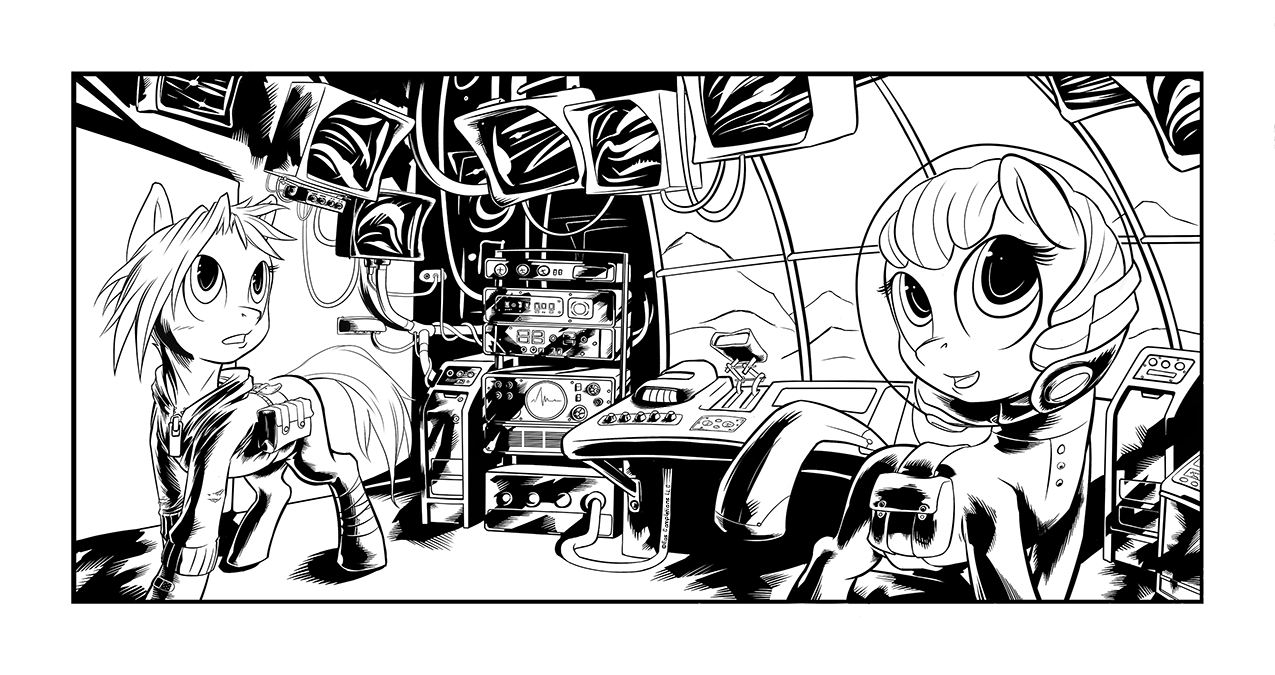
\includegraphics[width=0.9\linewidth]{image08.png}

\begin{intro}
那些床底下的黑影总让我担惊受怕。
\end{intro}

\daytimeplace{7}{3:00 AM}{旭日隧道,隧道镇}{Solaris Tunnel, Tunnel Town}

打了个哈欠,扳机低头看着幼驹在控制室地上玩。帕比正在一边用嘴发出『嘟嘟』声一边玩着一辆玩具车,她把一堆瓶盖放在车上,然后卸到一个闪闪可乐空瓶子边,然后再把瓶子装在车上。

「可以给我超级特别薄荷口味吗?好,谢谢,再见……」幼驹小声地玩着,好像她担心发出噪声惊扰到其他小马……

\thpr{她怎么做到的?把所有那些烦恼都丢在一边,然后就那样……坐下来玩儿?像个普通孩子一样?}

「喏,小家伙,你朋友怎么样了?」

帕比一边继续玩着她的玩具一边回答:「不知道,她说要花好一阵子呢,所以我要在这里等她……」现在幼驹似乎在用什么做一个围栏。

扳机吓了一跳,「你怎么还带着 \SI{9}{mm} 子弹?」

「哦,那些啊?闪闪发光的漂漂东西,而且好像有个揪耗毛兽强啥的要用。」小雌驹埋头玩着玩具。

「啥啥啥?」

帕比伸起蹄子大喊着:「吵吵的东西!」一把破破烂烂的九毫米半自动手枪出现在她蹄子上,吓得扳机连忙躲到一台终端后面。

「喂喂,谁给你那玩意儿的?很危险的!」

「才不,这东西吵死了……我也不喜欢,只有小雄驹才喜欢这种玩具的啦,除非它是粉色的话……」

女卫兵紧张地笑着,「对哦,帕比,那东西一点都不好玩,想换点有趣儿的东西么?」

这句话引起了帕比极大的兴趣,幼驹转过头来,水汪汪的粉色双眸闪闪发光,满怀期待的看着扳机。

「当然啊!你有什么?」

「呃,一个墨镜\footnote{墨镜:带墨镜的卫兵……黑杰克躺枪}如何?」

「好耶,墨镜!等等……」帕比皱起眉头,「我戴着这破头盔,戴不了墨镜的。」

扳机以蹄覆面,「好吧,抱歉小家伙,我想什么呢。」独角兽回头在她的鞍带里面翻着,「那么这本九成新的《缰绳八卦》杂志如何?里面全是漂漂马照片,还有小蝶的!」

帕比走到卫兵身边,看着杂志,然后开心地一蹦老高,「我喜欢这个,里面全是漂漂马!我认识这个,她是萍琪派!还有瑞瑞!哦哦,云宝黛茜!我超超超喜欢云宝!她可以飞在天上嘣嘣嘣!等我长大了我要当她的新娘子!我喜欢这个画册,给我嘛给我嘛给我嘛!」

扳机举起蹄子掩着自己嘴角的窃笑,「我想我们可以成交了,不过你要把子弹也给我。」

「好好好好!哦哦哦!这个大的子弹你能换给我什么?」帕比问着,又掏出一发大号的坦克用尾翼稳定脱壳穿甲弹头。

独角兽雌驹叹了口气,事情越来越麻烦了。

\horizonline

\daytimeplace{7}{3:00 AM}{糖霜咖啡馆,隧道镇}{Sugartop Cafe, Tunnel Town}

昏暗的咖啡馆里面现在烟雾缭绕,和每天夜里的这个时候一样,完全是个颓废的地方。几个醉醺醺的小马东倒西歪地躺在那里,吸着来历不明的药品,一只狮鹫躲在房间的角落,还有一只戴着墨西哥帽子的小马在弹七弦琴。酒保正在用一块黑得看不出颜色的抹布「清理」着地板,但是坏枪根本都不在乎这些。

「再来一杯!」他摇摇晃晃地举起空杯子,用力吸着里面的蓝色吸管,但是却发出空荡荡的吱吱声。「我说,你聋了么?我说再来一杯!」他不停地晃着酒杯但是谁也不搭理他,真是失望。

这里的酒保,那只黑鬃的银色公马,坐在他旁边放下一瓶闪闪可乐,「我说大家伙,安静点,客人在楼上睡觉呢!」

「闭嘴!老黑!」坏枪嘟囔着,「赶紧给我倒点儿给力的玩意儿,我真不敢相信她居然甩了我!」

年轻的伙计叹了口气,把可乐瓶推到坏枪嘴边。「拜托老兄,别惦记她了,赶紧睡觉去,你可以睡我楼上的床,别喝了,一点用都没有。」

卫兵看着他兄弟的脸,但是却不想从桌子上抬起脑袋来。

「你知道这酒吧有一半是我的么?」

「对,但是你每次来就是和我抱怨你过得有多悲催。然后呢,处理顾客,打扫卫生,撵走不付钱的醉鬼……」黑帽子在桌子上敲着蹄子,「老实说你帮我做了哪样?话说你自己就是个不付钱的醉鬼好么?」

坏枪挥着蹄子像是赶苍蝇一样嘘着他的兄弟,「滚边儿去老黑,你的臭气都快把我熏昏过去了,给我点新鲜空气。」

「那你为啥不去城外走两圈,好像坐在这里就会空气好一样。」

「闭嘴,再给我倒杯性感天马,老黑……」坏枪举着空杯子,脸却扎在桌子上。「她怎么可以……」

终于黑帽子发火了,「拜托,老兄,我知道你在说谁!就是那个快乐扳机,这是我见过最烂的婊……」

砰!

坏枪看着他趴在地上的兄弟,「老黑,你还真说错了,呆这里鬼混让我感觉到……嗯……非常好,」公马说着往外走,「谢了老弟。」

\horizonline

\daytimeplace{7}{3:15 AM}{旭日隧道,隧道镇}{Solaris Tunnel, Tunnel Town}

「帕比,你还记得……小马国两百……呃……在你离开中心城之前,那里怎样?」

小雌驹皱着眉头,想要想出个答案来。「新鲜!」

「新鲜?」

「没错,妈咪好像是某种士兵,但是她其实不喜欢打仗,她很擅长修东西,所以不是很危险的时候她都带着我。我见过很多神奇的好地方,比如说一个天马机场,还有地底下的一个叫避难厩的大地洞,但是完全不知道那是什么……而且我还到过小马镇,还有其它很多地方……」幼驹很自豪地抬头挺胸说:「不过52号国道的小马们看起来好可怜,这里没有青山绿水,也没有漂漂房子,小马们也都很不开心的样子。」

扳机感觉到有什么东西哽在喉咙里面,「如果……如果你不想说的话……就别说了。」

帕比看着独角兽,有些奇怪地回答:「为什么不想?虽然这里不如其它地方漂亮,但是这里也有很多大姐姐一样善良的漂漂马……或许等我找到妈妈可以带你去看那些漂漂地方……真的!我不知道为什么你们喜欢住在这种灰扑扑的地方。」

「呃……当然可以……不过……你可以先和我说说小马镇么?」

「当然!那可是我见过最漂亮甜美的小镇!那可是萍琪派去中心城之前住的地方!妈咪因为要去做很重要的事情所以让我在那里呆了整整一个暑假!我在那里交了好多朋友!而且那里的山丘和树木颜色都非常漂漂。哦哦哦,还有一个叫旋转木马的地方!但是并不是真的旋转木马,只是名字……」帕比皱了皱眉头,「我只告诉你哦,因为那个时候我问为什么那里的木马都不转圈圈,大家都笑了,而妈妈也抱起我笑,不过我却觉得自己超级蠢……所以……别问我为什么木马不会转哦。」

扳机咯咯笑着点了点头:「别担心,我不会问的。」

「然后那里的苹果园中间还挖了一个超级大超级大的水洞。哦哦,那里还有一个城堡一样的云屋,上面还有彩虹瀑布落下来!对了,还有个商店卖羽毛笔和沙发!」帕比看着扳机的表情,担心地问:「乐乐姐我说错了什么吗?为什么你哭了?」

「我……我没哭,只是眼睛进了东西……」

「哈喽!都给我乐起来,小姐们!P7来啦!」忽然房间里面的所有屏幕都变成了粉色,每个屏幕上都出现了好像七个气球捆一起的标记。

「你好,声音小姐!谢谢你能过来!」帕比对着最大的屏幕挥着蹄子,那里的气球已经被一行字代替。

「多谢你给我找的新家,帕比!这里比那个到处漏风进雨的破圆顶好多了!我们看看这里有什么……哦!地热发电机!维护机器马离线……这个简单……哦哦!还有好多好多秘密文件还有……呃……红色安全警报?我怎么忘了这东西?」声音暂停了一会。

「有什么不对吗,声音小姐?」

「没,只是我需要旭日公司的某个大头头的授权来解除警告,不过好像已经有某小马在程序上开了后门,所以我可以简单地绕进去,一会儿就搞定!」

扳机有点狐疑地看着屏幕,她从来不喜欢A.I.,但是这个看起来很友善,帕比也认识她,所以她决定还是等等看发生了什么。

而帕比已经完全放松下来了。小雌驹和往常一样天真灿烂地笑着蹲坐在大屏幕面前,「好的好滴,你现在能找到我妈妈是不是在附近么?超超拜托?」

「红色警报解除!所有系统正常,安全门即将打开,5、4……哦,我不知道帕比,这里的主机是个巨大的数据库,而且没有授权的话我不能……哦哦等等……我在这里找到『那一天』之后三个星期的数据……不过我需要一个密码……」

小雌驹举起蹄子,「我知道!快乐帕比!」

扳机叹了口气,「帕比,你的名字不可能解开所有东西,你知道……」

「密码正确,虽然这东西都放了有两个世纪了,我把它们显示在大屏幕上。」

幼驹皱着眉头颠过来倒过去地把这几行字看了几遍,然后泪汪汪地转回头来。

「帮帮忙……」

独角兽雌驹坐在帕比身边,然后用蹄子轻轻搂着她的脖子,「当然小家伙,我读给你听好不好?」

\medskip

\begin{center}
\textbf{第十八天}
\end{center}

\wrpr{如果我还有向塞拉斯蒂娅公主祈祷的权力的话,我真希望避难所科技的那些书呆子来做这些工作,而不是旭日公司的这群}

\medskip

% NOTE: 译文错误

「呃,骡子,没错帕比,就是骡子……」

\medskip

\wrpr{这傻蛋旭日公司还真搞出一个在紧急状况下把优先权赋予技工的协议。但是这帮蠢货居然忘记给机器卫兵设置敌我识别!}

\medskip

「呃,这个词没啥意思,帕比,我们继续……」

\medskip

\wrpr{至少隧道现在还安全,我会在这里扎营几天,然后收集一下补给品为穿越沙漠做准备。}

\wrpr{已经快凌晨两点了,但是我睡不着,我好想她!我知道她在避难所里面很安全,但是我还能听到她因为怕黑和做恶梦拼命叫我的名字,但是我醒来却发现只是个噩梦。}

\medskip

「胡扯……嗯,是的,胡扯。」

\medskip

\wrpr{我应该给自己找点儿事干,免得我发疯,我恨小马国}

\medskip

「嗯,这部分是向女神的小小祈祷。」

\begin{flushright}
\textbf{阴雨·黛丝}
\end{flushright}

\medskip


扳机叹了口气,\wrpr{阴雨·黛丝女士写这个的时候,她绝对没想到她的小女儿真能读到这个东西}。

「好吧,看起来她继续往南走了……我们继续看看下面的记录。」

 P7打断她们的对话问道:「喂,帕比,你记得沙盒主任的密码么,超超拜托!」

幼驹戳着自己的头盔思考着。「玛塔莎?不对……是阿加莎!」

「谢谢啦,亲,我超超超想给你个大拥抱,让我们做做看吧,你先抱一下你自己,然后就当是我抱的好了!这里还有第二个文件,我会去我不该去看的地方转转看,你们好好玩儿,别弄得一团糟哦。」

\medskip

\begin{center}
\textbf{第二十一天}
\end{center}

\wrpr{我终于准备出发了,看起来没有其他小马来这个方向,我难道是这里唯一的幸存者?不太可能,但是我不想赌自己的运气,我打算绕开太阳城,这里被核弹头密集轰炸过,昨晚我都能在沙漠中看到那诡异的辐射光。如果我走运的话,几天之后我就能走到蓝羽机场了。我一天亮就出发。}

\wrpr{我还是睡不着,我一直梦见帕比死在厨房的地板上……}

\medskip

「胡扯,帕比,胡扯……」

「你喜欢胡扯么?」

「好了好了我继续读……」

\medskip

\wrpr{这只是噩梦,我很确信她很安全,她从来没有不听话过,为什么我一直梦到她?我找到一些药片,其中一些可以当安眠药,如果再做噩梦的话我就吃点儿。}

\begin{flushright}
\textbf{阴雨·黛丝}
\end{flushright}

\medskip


帕比紧紧地抱着卫兵,头盔紧紧压着扳机的后背。

「怎么了小家伙?她只是想你了,你现在好得很,等你找到她之后你就没事了,她也不会做噩梦了,对吧?」

和幼驹扯这种毫不羞耻的谎话让扳机的内心如同刀绞,但是帕比现在需要安慰。

「我……我不是好孩子,乐乐姐……我没有去那个秘密地方,因为我想去看烟花!」幼驹大哭起来,「我是坏孩子,妈妈会生我气的!」

扳机转身抱起小雌驹,安慰着她,「好了好了,别担心,你妈妈说了她要往南走,对吧?去一个……什么蓝羽机场?……我想那里就是铁锈庄园了,去那里很简单,只要绕过太阳城就到了,她再见到你一定很开心的!」

\thpr{为什么我要给这个可怜的小家伙希望?她妈妈早已经死了,我到底在做什么啊!}

那双清澈的粉红双眸中燃起了新的希望,帕比凝望着雌驹,「真的?她会在那里吗?」

「我……我也不知道她是不是,不过你想要追上她吧,对吧?如果你想要寻求真相,你必须跟着她新的足迹继续前进!」\thpr{没错,乐乐,两百年前的新足迹。}

幼驹又一次笑了起来:「对!我去什么地方都没关系,跟着妈妈,我去什么地方都可以!谢谢你乐乐姐姐!你是最棒的小马!」

 P7又一次打断了她们,「非常好,我搞定这里的物品清单了,好像旭日公司的家伙早就开始为『小马国末日』做准备了,这里有好多实验室,而且还有足够的军火再给那些幸存者来一次烟火秀!哦哦,帕比,我想你刚才又把萍琪派的名字给念错了!」

帕比抬起了头,「啥米?」

「简单的说,朋友,在这个山下面有好多好多层仓库,装满了各种军火,那些东西足够把小马国上的每一个混蛋都杀死两次!」

「呃……你说『杀死』是说,伤的很重?」小雌驹狐疑着问。

「不对不对!我是说伤得超级重!就像一个所有小马进去以后就出不来的超级大派对!」

「一个……机器萍琪派对?」帕比不由得打了个寒战,完全不想听到之后的回答。

「机械萍琪:文件未找到。」

帕比想了想然后又问:「好了,那么这些东西有些什么呢?」

「我们举几个例子吧!比如说『长程多弹头电浆导弹』这玩意能分裂成56个弹头同时命中56个不同的目标,每个弹头都可以轻易击穿地下防御掩体,然后把整个密闭空间灌满电浆,把温度瞬间上升到几千度,杀死里面的所有小马!还有『广域解离射线发生器』,可以把一百米之内的所有目标分解成原子状态,当然也会杀死小马。哦哦,还有『巧克力混沌\footnote{巧克力混沌(Chocolate chaos):正剧 S02E01,无序躺枪}』这个魔能武器可以把目标的血液变成巧克力牛奶!虽然效果会在一个半小时后消失,不过被打中的马当然也是立刻就死翘翘啦!」

「好了好了,不用说了……」帕比打断她的话。

「那么,我们该怎么办?你是老大!」

电脑最后一句话的话音刚落,扳机连忙举起蹄子想阻止小雌驹说出任何蠢话,不过她还是不够快。

「把它们全扔了!挖个大洞把那些东西都丢进去,在上面盖个房子然后把这里的所有坏蛋机器都送进去,这样就不会有小马受伤了!」

「好吧,从技术上讲,所有东西已经在这个山下面的大洞里面了……我可以炸毁通向仓库的电梯,除非有谁把整个山都挖开,否则他们肯定找不到那些东西了。」

「就这么办!」

扳机松了长长一口气。

\horizonline

\daytimeplace{7}{3:30 AM}{隧道镇,52号国道北口}{Tunnel Town, Big 52 N Branch}

坏枪用头撞着隧道的大铁门。

「肏,肏,我应该阻止她的……肏,肏,肏肏肏!」

「我说,老哥,就算你用力踢它,门也不会奇迹般地被你踢开的。」黑帽子坐在卫兵身边揉着眼睛,「我想这个乌眼青是我自找的,不过……这不代表我哪天会打回来。」

「看在露娜的份上,老黑!拿个腌青鱼压着那眼睛睡觉去,让我自己静一静行不行!」

银色公马靠在墙上打着哈欠,「没门儿,我才不会把我兄弟丢在这里,而且,这件事足够我笑话你几个月了。」

坏枪怒气冲冲地喷着响鼻,「我总怀疑我们老妈是个婊子,现在我很确定了,乐乐都已经不在了你还想笑!你是想再多个黑眼圈还是现在就滚蛋?」

「冷静点吧,你现在啥也做不了,这东西封得……我勒个去!」

一阵尖锐的金属摩擦声之后,大门缓缓升起,让黑帽子一屁股坐在了地上。

「我勒个大去……」

俩小马一脸难以置信的表情看着巨大的钢铁怪物——两米厚的巨大防水板慢慢升起,然后后面的另一扇隔板也缓缓让开。

坏枪傻站了快一分钟才张开嘴。「这……我……没做梦吧?掐我一下……」

砰!

「你这个尸鬼养的……我是说掐一下!」

老黑窃笑,「我说了你欠我一下,你还说她已经死了?」

两只雄驹蹄下跨过骷髅走进山洞内,黑帽子看着满是子弹孔的马车,又看着里面装的东西。「哇哦!这么多好东西!这小镇要发财了!」

坏枪则稍微走得远了一点,看着隧道的灯一盏一盏点亮,开始照亮这六公里长的地下隧道,而天花板上的一处通风道还挂着一根绳子,于是他撒开蹄子飞奔向山洞深处。

「等等老哥!别跑那么快!我们要叫上其他卫兵!」

「去你妹的卫兵!我喝高了而且还恋爱了!」雄驹的声音回荡在隧道中。

黑帽子叹了口气,跟着一起追了过去,「至少你等等我呀!」

\horizonline

\daytimeplace{7}{9:00 AM}{隧道南贸易站,52号国道中段}{Trade Station Tunnel South, Big 52 SC Branch}

扳机抱着帕比亲着她的头盔,而后者一脸不耐烦地拼命挣扎着。「唔……好肉麻,别在那么多小马面前亲亲!」

所有城镇卫兵和隧道镇的许多其他居民都围住了他们。在扳机护送着帕比走出隧道南口的时候,一位代表小镇政府的雌驹发表了一个小演讲,并且送给帕比一袋子瓶盖。

在两只小马面前是无边的地平线无数的沙丘,偶尔有几个红色的山石出现在视野中。在远处能够清晰地看到一个城市的剪影,但是沙漠的风尘让大家难以辨识这是真实的景象还是海市蜃楼。

「帕比,我们到了,这就是蛇蝎沙漠,你好好听我说怎么去铁锈庄园。」

小雌驹乐得蹦蹦跳跳的,「没问题,漂漂乐乐姐!」

「很好,这个荒漠是清砂工的领土,他们大多都是住在各种各样帐篷的拾荒者,在沙丘下面寻找各种有用的东西,不过我还是要提醒你,他们有时候还会抢劫,尤其是对于独行的旅者,但我觉得他们恐怕没那个胆子敢抢劫你,毕竟清砂帮是个非常迷信的氏族,而且他们肯定从孤狼那里听说过你的事了。」

帕比点了点头,「喜欢走来走去的漂漂马,懂了!」

扳机笑了笑,「很好,你只要跟着路标,很简单的,因为每隔50米清砂工就会放一面红色旗帜,你只要跟着旗子走,就能在明天早上之前到达他们的第一个营地。」

帕比皱着眉头指着旁边坚实的柏油马路,「为什么不走大路?踩着我的滑板在路上就像飞梭一般!」

「不行!小家伙,这个公路是直接通往太阳城的,你绝对不能去那个地方!」

「为啥?」

「那里是个危险的地方,所有小马去那里就再也没回来过!」扳机的声音中带着不容置疑的口吻,但是帕比完全没有在意。

她敲着自己头盔下巴的位置,「呃,或许他们超喜欢那里,所以不想走了呢?」

「我……我可不觉得……帕比,当我还是你这样的孩子时,太阳城是另一个氏族的地盘——锈刃,他们和清砂工是同盟……那是很久之前的事情了,但是后来听说清砂工找到了什么大家伙,而锈刃偷走了,然后就是说谁背叛谁的,最后他们就打起来了。最终清砂工想要策划一次突袭,在晚上夜袭城市。」雌驹顿了顿,看看幼驹还有没有在听。

「然后呢?」小听众有些担心地问。

「在突袭中发生了什么灾难,但是谁也不知道究竟出了什么事,只知道清砂工带了他们的所有武器冲进城市,但是却谁也没有回来,所有想要调查城市的小马都消失了,然后清砂工把剩下的小马聚集起来——大多都是老马和孩子,现在还在沙漠中挣扎求生。」

「所以,他们都是大坏蛋?」

班级皱了皱眉头,「在废土可没有什么明显的善恶之分,帕比,如果你想活下去,有些时候你必须做出一些……牺牲……就算是心碎也好,总比彻底失去生命要好。」

「呃……啥?」幼驹一脸茫然地看着扳机,不知道她话语之中的哲理。

「好了,别瞎想了小家伙,你就觉得……好吧……他们是坏蛋,但是他们不是自愿的。」

帕比摇了摇头,「不对!如果你做坏事,那你就是坏蛋!没有借口,如果觉得小小坏事就不算是坏事,那你最后就会做出大坏事,变成一个超级……超级大坏蛋!」

「呃……你自己想出来的么?」独角兽钦佩地看着帕比。

「才不是咧!妈妈说的!」

扳机拍拍帕比的头,看着她担心的表情,「别担心,打烂机器马不算坏事,妈妈不会不开心……好啦,笑一个!」

黄色的幼驹开心地跳上滑板车,「我见到妈妈以后会告诉她你对我超级好!谢谢你漂漂乐乐姐姐!」骑着滑板车,幼驹顺着沙漠的公路绝尘而去。

「呀呵呵……」

扳机看着幼驹骑着滑板越来越远,然后叹了口气,「我很抱歉,小家伙。」

「那么,乐乐,那就是那个小幽灵?」坏枪走到雌驹身边笑着问。

「我不知道,」扳机叹了口气,「我只知道她是个迷路的孩子。」然后她转头看着公马笑了起来,「你那熊猫眼哪里来的?」

「兄弟情谊纪念。」坏枪哼了一声,然后又说:「我们何曾不是迷失在这个残酷的世界之中呢?不过我想新闻一发出去的话,很快就会有大批小马来隧道镇了,我们要增招卫兵。」

「说到那个……马车上的货物应该回收,那些东西应该平分给每个小马,你帮我看好黑帽子。」

公马点了点头,「没错,别担心,其他小马已经把车拉回城了,有些车还是有标志的,有三个属于水头,还有一个是旋转木马的,不过上面的东西已经被和机器卫兵对干的小马糟蹋得差不多了。我们还给他们吗?」

「我们应该还给他们,至少作为我们善意的象征,他们知道我们帮他们保管好货物的话,也会乐于和我们合作的。哦,顺便提醒了我要教教你如果通道再次关闭的话该怎么打开。」

坏枪迟疑了一会之后又追问道:「还有,那个……昨晚那个……你知道的……在你追那个幽……帕比之后,我和你说了些……然后我们……能假装……我们什么也没说么……你知道的……那个……啥……」

扳机咯咯笑起来,「我可不觉得,大情圣……那可是我见过最笨的告白了,为了那些话,我也要和你过下半辈子啦。」

坏枪低下了头,「呃……我可以问问为什么吗?」

「我可以先问你一个问题么?」

公马挥着蹄子,「当然……问吧……把爱心之箭射入我心房吧……」

「我还有机会说……我也爱你吗?」

\horizonline

\daytimeplace{7}{4:00 PM}{蛇蝎沙漠,52号国道中段}{Serpent Desert, Big 52 SC Branch}

{\rt 女士们,先生们!下午好!这里是孤狼的52电台!小马国这片区域最好也是唯一的电台!昨天我正在街上走然后有小马问我,为什么大家都听你的节目?你的节目怎么会这么好?好吧,我必须承认那个不简单,因为我可是这附近唯一一个肏蛋DJ了。}

喇叭里一个女性在远处说:「{\rt 耶!!没错!}」

{\rt 坏孤狼,你说脏话了!你不应该说脏话的!尤其是我们的小英雄还在听你的节目的时候,对吧,对吧!我是个坏蛋我应该害臊才对。不过现在我却觉得很高兴,不,是非常高兴!因为一个带翅膀的朋友刚给我从南边带来了大新闻!做好心理准备,听众们,因为这个新闻超级劲爆!}

忽然随着一阵静电干扰声,广播中断了几秒钟,但是马上就恢复了。

「{\rt 好了,听众们我又回来了!你们竖起耳朵听好!谁也关不掉52电台,特别是今天,因为今天我们要一起庆祝隧道重新开张!没错小马们!你们耳朵没撒谎!隧道镇又回来了!再也不用走山路了!}」

狂野的音乐持续了一分多钟,而DJ在背景里面用嘴模仿着吉他的声音。

「{\rt 这可是砸烂嘉年华之后最大的好消息,猜猜是谁干的?没错,我们的守护天使!我们的小小幽灵!我们需要一个小孩子把我们从濒临饥荒之中拯救出来吗!肏你妈我太失望了!不过不开玩笑,一个小孩子,一个星期不到的时间,就把三个城镇从他们最恐怖的噩梦之中拯救出来了!一个小孩子而已!我说52,你们的骨气都哪儿去了?给我看看你们的信念!别让我一直崇拜一个比我小好多好多的小孩子行不行?}」

一阵沉寂之后,DJ的声音又回来了,这一次显得疲惫不堪。

「{\rt 醒醒吧伙计们,她只是一个孩子而已,她不可能搭救所有的小马,我们应该振作起来,我们自己就可以做得更好,我们不需要另一个英雄来崇拜!}」

一段悠扬的吉他声之后,另一段音乐响起,不过这次不是录音,而是孤狼自己唱的歌。

\begin{music}
走出废墟,走出残骸

\begin{englishlyric}
    Out of the ruins, out from the wreckage
\end{englishlyric}

\medskip

我们不能再犯同样的错误

\begin{englishlyric}
    Can't make the same mistake this time.
\end{englishlyric}

\medskip

我们是新一代的子女

\begin{englishlyric}
    We are the children, last generation.
\end{englishlyric}

\medskip

我们是被遗忘的一代

\begin{englishlyric}
    We are the ones they left behind\dots
\end{englishlyric}

\medskip

我们要改变这个时代

\begin{englishlyric}
    And I wonder when we are ever gonna change it,
\end{englishlyric}

\medskip

在恐惧和余烬之中挣扎求生我们一无所有

\begin{englishlyric}
    Living under the fear till nothing else remains.
\end{englishlyric}

\medskip

但是我们不需要更多英雄

\begin{englishlyric}
    We don't need another hero\dots
\end{englishlyric}
\end{music}

\horizonline

「哇哦,我真想见见他们说的那个超级英雄小雌驹!你觉得我们可以做朋友吗?」帕比跟着红色旗子在沙漠上走着。

「{\mt 肯定,通常英雄偶像都是相当友善的。警告,检测到中等辐射,威胁等级:可忽略。}」

幼驹一边走着一边问着:「对了,声音先生,你觉得我是好孩子吗,我妈妈还喜欢我吗?」

「{\mt 警告,该程序没有社交功能。}」

帕比长叹一声,「老天,每次问到关键问题你就躲起来,是吧?」她正想在说点什么,但是她的注意力被远处一个影子吸引了,「看,有个漂漂马!」

这个「漂漂」马看起来是一只鬃毛花白的红色独角兽,一件宽大的披风遮盖住了她的全身。当小雌驹走近的时候,她笑了,「慢慢来,小幽灵,我在中午就在这里等你了。」

「嗨,我是快乐帕比!」小雌驹挥着蹄子笑着说:「我很抱歉我迟……呃,我哪里迟到了?」

老马的嘴角微微挑起,「当然是探险……你喜欢探险吗?」

「是啊!我超超超爱探险!哪里可以探险?我能来两个吗?」忽然幼驹的表情变得严肃起来,「不对……等等……我还要找妈妈,不应该去探险……」

老马笑了笑,「没错,你已经有自己的路要走……我怎么忘了这个。」

帕比点了点头,「没错,我很抱歉,我该走了,谢谢,拜拜!」

「不过,如果我说这次探险是关于你的一个陷入危险的朋友呢?」

已经走开的幼驹又回过了头,「我的一个朋友?谁啊,为什么,在哪儿,什么时候?」

「好了,别急……」

帕比跳上长者的后背,用她的头盔贴上了她的鼻尖,她紧盯着独角兽的眼睛。

「拜托拜托快跟我说!」

老独角兽一下子没站稳,差点摔倒,「冷静一下,小幽灵,我正打算和你……快坐下听……好不好?乖乖的我就和你说话!」

「呃……好的……很抱歉漂漂老奶奶……」帕比放开她的脖子然后坐在独角兽面前,而后者松了一口气。

「我是先知长耳,一个可以看到远处景象的小马。」

帕比蹦蹦跳跳地说:「哦哦哦,你能看到我妈妈么?她能看到我们吗?她还好么?」

「不是那样的。」

小雌驹一瞬间泄了气坐了回去。

「我吃一些药之后,我可以在梦中看到一些景象,但是我不能选择我要看什么,昨晚我看见的是关于你的梦境。」

帕比安静地坐下来,在沙漠当中听着长耳慢慢讲故事。

「你让一个非常重要的朋友为你做一件很重要的事情,你的朋友竭尽全力,但是发生了一件非常糟糕的坏事,她没法再继续她的任务了,所以她在我的梦中让我来转告你。」

帕比皱了皱眉头,一个很重要的朋友帮一个大大的忙?但是她从来没有——哦哦,是丝尾!她让它照顾赫瑞别让坏事发生在她身上!

「赫瑞?她有危险?在哪里?」

雌驹点了点头,用蹄子指着远处的太阳城,「我恐怕那只小鹰飞得太靠近太阳,所以找不到回来的路了。」

帕比犹豫了一会,「但是……乐乐姐告诉我不能去那里!我要听她的话!」

长耳耸了耸肩,「你并不是非去不可,你让朋友帮忙,而她让我警告你,就是这样,你可以选择不管她,然后继续你的旅程。而我的任务也就是这样。」

「但是……但是有什么坏事发生在赫瑞身上!我不能把她丢下!她可能会受伤!她可能会哭!」

「那么,去太阳城救她吧,但是我要警告你,太阳城是一个陷阱,是个真实的噩梦,当你开始做梦之后,你就不能再离开了。」

「这个别担心,我一点都不困!」帕比笑得别提有多轻松了,「太空战士安德洛队长前去营救啦!」幼驹向城市奔去。

长耳看着飞奔的黄色幼驹,直到她远到化成一个灰色的小点儿,然后拿出一个药片,就着一瓶奶白色的液体吞了下去。但是老马能看到的只是火焰和枪声,

「我看到的是什么?过去还是未来?」

咯咯笑的声音在老马耳畔响起,「她很精神,一直在笑,我喜欢她!如果大家都能像她这样,不是一直板着脸的话……」

母马低语着:「但是一个梦魇能带来和平么?我不确定……」

「别问我啦!我只是你的迷幻剂带来的一个幻觉而已!真的,我帮不了你什么!就算你不看它,事情也会发生,而且你也不知道这个是过去还是未来。」

老独角兽叹了口气,「或许你是对的……我们回家吧。」

「对,我们走吧,帕比会照顾好自己的!」

~\vfill

\begin{note}
升级(Lv 7)

新技能解锁:钢铁力量——有时候光是石头还不够,你使用的所有钝击武器都增加5点额外伤害(没错,石头和动力蹄都属于钝击武器)。

任务技能:52之魂——你的传说在52号国道上流传,只要大多数氏族和你的关系保持中立或者中立以上,你随机遇到的低级敌对目标就会减少。
\end{note}


\chapter{太阳城}

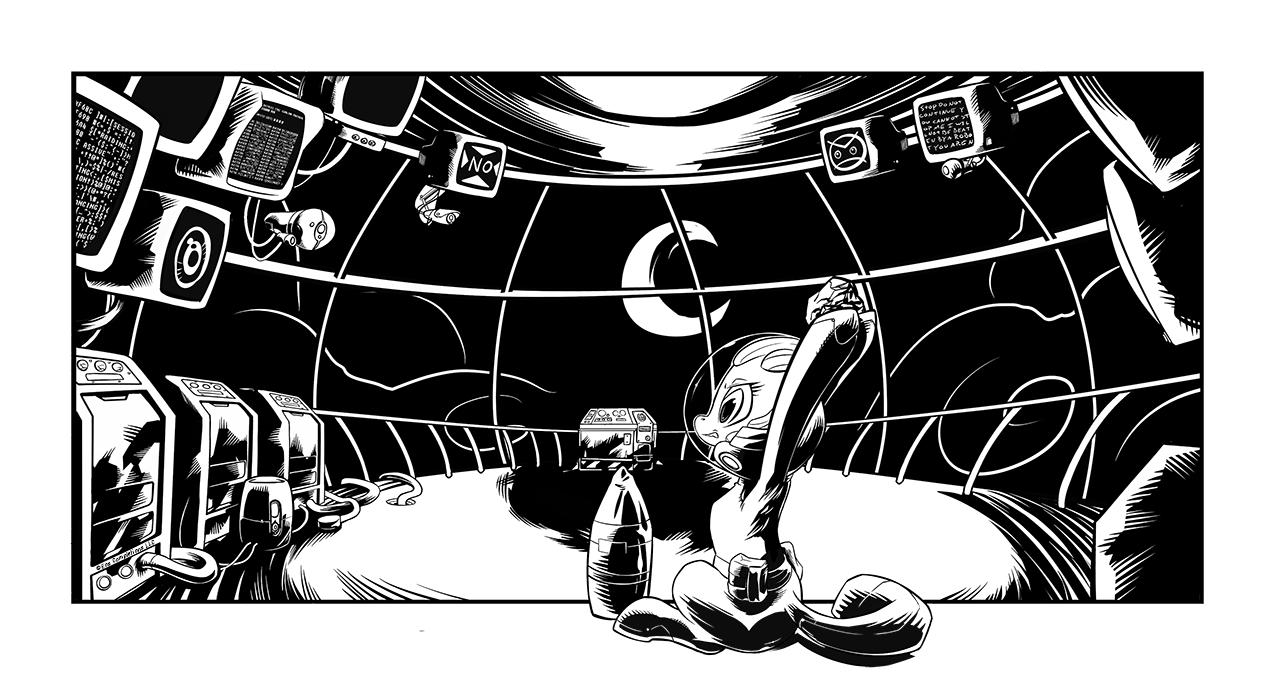
\includegraphics[width=0.9\linewidth]{image09.png}

\begin{intro}
太阳城不只是一个小镇,它是小马们罪孽的救赎。
\end{intro}

\daytimeplace{7}{11:00 PM}{太阳城郊外,52号国道中段}{Sun City Suburbs, Big 52 SC Branch}

去城里的路非常远,帕比走到第一个房子边的时候,夜晚的黑暗已经笼罩了街道的每一个角落。太阳城中心社区被一大堆小小卫星城区包围着。但是每个窗户都黑漆漆一片,半点光亮也没有。帕比走过的建筑看起来都已经被拾荒者洗劫一空,只剩下一个个房子尸体般的空壳,就像是一片坟墓,一片曾经被叫做「家」的东西的坟墓。

帕比并不想承认她还有点怕黑,但是这个空旷的地方让她想起来小时候的各种鬼故事,「为什么小鸡要跑到这么可怕的地方惹麻烦?笨赫瑞!这里什么都没有,为什么还叫『城镇』?」

随着深入这个可怕的地方,帕比开始好奇,那些五颜六色的标志都去哪里了?虽然她没怎么在夜晚出去过,但是她很确定夜晚的城市不是这个样子……她想要一些音乐以此盖过夜晚阴风吹过空洞房屋发出的哀嚎,但是无线电一到太阳城附近就没有声音了,让帕比感觉到又孤单又害怕。「呐,声……声音先生……你还在吗?」

回答帕比的只有一堆毫无意义的沙沙声。

「{\mt 兹兹……危险……沙沙沙……变……兹兹……电……沙沙沙……可能\\……哔哔……影响……哗哗哗……思考。}」

% NOTE: 强制断行

「唉,他又生气了……」幼驹皱着眉头继续走着,头盔的HUD开始显示文字的警告信息,但是密密麻麻的字幕活像是蚂蚁,而且滚动速度快到帕比根本没办法看清。小雌驹觉得自己孤立无援——无线电坏了,声音先生不见了。就像那些可怕的夜晚,她想要睡觉但是屋子太黑太可怕,她不停地叫着妈妈,直到妈妈过来抱起她抚摸着她,把她哄安心。帕比想要唱点儿什么壮胆,但是在这种黑漆漆的地方她只能想起「邪恶女妖」啥的歌,完全没有什么帮助。

帕比走过迷宫一般空旷的街道,蹄声的回音让她觉得毛骨悚然。每一个空洞的窗户都反射着她双眸里明亮的粉色鬼火,那是什么?或许马尾伯爵又从坟墓里面爬出来了?而且她觉得这个时候就连马尾伯爵都不那么可怕了……远处传来一阵不可状名的尖叫声吓得幼驹僵立在原地,她后蹄一软直接坐在了马路上。

「那……那……那……那……那……那……是啥?」

打烂坏蛋机器和追着妈妈一点都不可怕,而尸鬼小马虽然看起来很惊悚但是她至少知道自己可以打什么……但是这里完全不一样——一个空无一物的城市,到处都是闹鬼的房子和发出怪声的街道,她为什么想到鬼怪幽灵?不要幽灵!坏幽灵!为什么她要离开红旗子的小路,漂漂姐姐明明说她不要离开那条路,但是她必须来这里帮那个笨小鸡。但是现在这里又黑又可怕,帕比超想念丝尾小姐。

小幼驹趴在路上耷拉着耳朵,尽力假装自己是路上的一块石头。

「新……新……新……新……计划!我们在这里等明……」

另一阵声音在空旷的街道回响着,好像是幽灵的哀嚎一般。

「……天……啊啊啊啊呀呀呀呀!」帕比撒开四蹄,风驰电掣,就像在落叶赛跑上的云宝黛西那样一溜烟飞奔出去。

「新计划!我们出城等天亮!」

\begin{center}
太阳城1分——帕比0分
\end{center}

\horizonline

\daytimeplace{8}{8:00 AM}{太阳城郊外,52号国道中段}{Sun City, Big 52 SC Branch}

天亮之后,这个城市看起来和盐块城差不多,甚至比得上中心城,一点儿也不可怕……就是有点儿……呃……丑。帕比在想为什么昨晚自己那么害怕,她真是个笨小孩。

「看吧,声音先生,这里没什么好怕的!就是另一个城市,到处都是破房子和烂马路还有……」帕比忽然看见有什么东西从头上飞过,「还有漂漂翔马们\footnote{翔马们(Peggysuses):天马这个单词的复数就连很多英语母语的人都会搞错}!好棒!」

幼驹撒欢跑了起来,追着那个飞行的影子。「喂!喂喂喂!漂漂翔马们等等我……等等噗……」抬头看着天跑的小幼驹完全没有看前面,径直撞进另一个走在街上的陆马怀里。

「哎呦……你为什么不看路啊!我先从这里跑的!」

那个棕毛黑鬃的成年陆马似乎正背着一大堆砖块和其它建筑材料,不过现在已经被帕比撞得散落一地,帕比心中一惊然后立刻打算在那个老马生气之前溜走,但是他只是低头开始默默地把砖块捡回去。

「哼!这下知道教训了吧……别站在路中间和一个笨雕像一样!」帕比吐出舌头做鬼脸,但是她发现那个陆马根本没有在意她。他看起来只是有点……怎么说……

「呃,抱歉先生,您没听到么,我是快乐帕比,我在找我的妈妈……虽然通常是这样,不过今天我是来救我的朋友赫瑞,听说她在这里惹上麻烦,但是我又不知道是什么样的麻烦,你有看到她么,她有一个喙而且长着毛,看起来像是一只小鸡但是又不喜欢我叫她小鸡,但是我叫她小鸡又不是她想的那个小鸡,不管怎么说她都看起来像是小鸡,对了哦,我还见过斑马,我不知道为什么小马都不喜欢斑马而且那个斑马也不喜欢我们叫她斑马或许这就和小鸡不喜欢别人叫她小鸡一个道理……」

帕比紧紧跟着那个陆马,但是陆马却一言不发的,他捡起掉下的所有东西,然后走向城中心。帕比可以看见清楚看到那些完全被搜刮一空的房子似乎是城市的外围,就像是大概200米左右的无马区,但是城市里面却不一样,似乎小马们正将城市外面的房子一砖一瓦地拆散,然后再修葺好城市中心的房屋。

帕比停下来,看着面前这个在晨光中冉冉发光的城市赞叹道,「哇哦,你们还真有个漂亮的小镇!超赞!」

就在小雌驹面前展现的是如同往昔记忆之中的城市一样——有很多粉刷得很漂亮的小房子,屋顶上有门洞,门上也没钉着木板,各式各样的小马搬着各种东西忙碌着,看起来是个非常活跃的社区:大家都在忙着做什么事情,就算是幼驹和天马也是,有漂漂房子,漂漂飞天马车,就算是花园看起来也不是枯黄而是翠绿色,甚至还有绿树!帕比觉得这个地方完全可以打60分,不过,不管怎么说这可是这么长的旅途以来,第一个她觉得值得打分的地方!

「乐乐姐绝对大错特错!」帕比跟着她刚刚撞上的棕色小马,「小马真的是太喜欢这里所以不想回去了!事实再一次证明人家的正确性!哦哦,对了,说起来乐乐姐……呃……你好像不怎么喜欢说话……」不是不怎么,是完全不说话,所以帕比决定还是不管那个陆马,自己在这里逛逛。这个非常漂亮的城镇让她想起了妈咪带她去过的一些小镇,在废土游荡了八天之后,终于找到了一个美丽的小镇——即使这个小镇的小马都有些奇怪,让帕比觉得莫名其妙。

黄色的幼驹开始在这个城市里面探索,她看到一个狮鹫正蹲在屋顶上换着坏掉的瓦片,于是她大叫起来。「嘿!小鸡小姐!你看到我的朋友赫瑞了吗?她也是个小鸡!」但是,完全没有回答,这个地方的小马不是全都聋了,就是都非常不友善。

然后帕比看到一个独角兽雌驹正在给树浇水,于是她走过去,「打扰一下漂漂姐姐,请问您看到一个叫赫瑞塔的小鸡吗?」还是没回答,幼驹开始觉得不耐烦了,很明显她一直没什么进展,「呃,她另一半是猫咪!」

独角兽丝毫不管帕比继续浇着水。不过帕比这一次绝不会这么简单放弃,她亲自走到了那个独角兽和树之间,直视着她那双……斜眼?

「呃……你的眼睛……好奇怪?」

那雌驹一脸茫然地斜眼呆立着,「你怎么做到的?」帕比好奇地坐在地上看着她,「怎么让两个眼睛同时去看不同的方向?」

幼驹又一次被完全忽略,雌驹转身想要绕开帕比,但是黄色的幼驹坚持不懈地站在独角兽和树之间,最后她直接把水浇在了帕比头上然后走开了。

帕比现在又湿又不开心,「我说,这样很不礼貌耶!这里的小马都怎么了?为什么不和人家说话?是我身上臭臭吗?」幼驹低头嗅嗅自己身上,但是她穿着防护服一点意义都没有。

幼驹继续在社区里面转了一上午,想要找到谁可以和她聊天。但是这里的每一个小马都一样,一脸斜眼白痴表情,而且完全不听她讲话。

帕比想起以前她妈妈不让她看的那种奇怪电影,地铁二零几几什么什么的……不管怎么说她偷偷看了,而且无聊得要死,这个城市也一样,就像之前那个狂欢到真的让你死的农场一样,这里是无聊到真的让你变石头的地方。

她继续深入探索着这个城市,虽然路上偶遇几个和帕比年龄相仿的幼驹,但是他们也一样只知道工作,完全没有在玩,帕比真的努力去交朋友了,她试着和他们玩钉马尾或者更有趣的游戏,比如说扮太空小马和番茄星人,但是那些孩子就是不理他,现在帕比觉得又寂寞又伤心。

「声音先生走了,赫瑞又不知道去哪了,这里的小马都装傻不理人家!这里是最烂的城市!如果一点乐趣都没有,要那些漂漂房子和绿树有什么用?为啥大家都这么奇怪?」帕比叹了口气,她想起来每个小镇都应该有一个镇长或者什么管事的小马,或许问他的话可以找到一些答案,这些小马一般都住在市中心之类的地方,在太阳城这里是在明显不过了——那些摩天大楼显而易见是市中心。

「看起来超简单!」帕比蹦蹦哒哒地走向那边,但是却发现自己正漂浮起来远离自己的目标。

「哎?」

幼驹转过身才发现有个成年小马叼着她的后脖子,就像抓小猫一样把她拎出城去。

「喂喂喂!放开我坏蛋!我想要去那个闪亮亮的高塔!我要见市长!超重要的!你这个斜眼笨蛋!你有听我的话吗?」

那小马把帕比丢在了城市边缘的荒芜地区,然后留下在那里大喊大叫的小幼驹走开了。

\begin{center}
太阳城2分——帕比0分
\end{center}


\horizonline

\daytimeplace{8}{2:00 PM}{太阳城,52号国道中段}{Sun City, Big 52 SC Branch}

帕比一脸凝重的神色看着那些忙碌的小马思索着:他们不想让她走进城里,但是她必须想办法进去……或许她需要一点聪明的『战术』比如说穿个墨西哥宽边帽和斗篷之类的?恩……这个点子似乎不错,但是现在去哪儿找个假胡子呢?

忽然,幼驹的注意力被一个天上飞过的影子吸引了,她早已经习惯了天马在天上飞来飞去,不过这次不一样,是一个狮鹫,一个穿着熟悉铠甲的小小……「赫瑞塔!喂喂!赫瑞……等等!」

不过即使是她的最好朋友也不理她,帕比虽然不太开心但是她正忙着想办法引起赫瑞塔的注意,于是她大喊:「石头!」「命运之石」出现在帕比蹄子上。

她摆了一个Pose慢慢瞄准,然后……「咻……」「正中靶心!」狮鹫发出一声惨叫然后从天上栽下来,就像是……呃……被石头打中一样。

「别担心,赫瑞,我在下面接着你呢!」

帕比飞奔起来,想要在她满是羽毛的朋友坠落之前接住她,同时赫瑞塔正在拼命地想要从失速状态改出,但是她被砸得晕晕乎乎的脑袋完全没办法反应,她只能瞄准一个看起来软乎的东西做落点……对哦,那个黄色的小点进入了她的视线,一个不停地喊叫和奔跑的小黄点。

「我接着呢,我接着呢,别担心我……」

噗……「哎呦!」

「哎呀!」

狮鹫晕晕乎乎地看着快乐帕比,然后大叫起来。

「帕比肏你娘的,你丫在这么危险的地方闲逛个屁啊?还不快给老娘滚!如果听到那个嗡嗡……」赫瑞塔忽然也变成了斜眼,然后不说话了,一缕血丝顺着她头上的伤口流下,她也没反应。

「赫瑞,终于找到你了!丝尾告诉我你有危险但是……嘿!你想去哪儿啊?」狮鹫张开翅膀,然后准备起飞,但是黄色的小雌驹紧紧抓着赫瑞的脖子不让她飞起来,「别想逃掉!我们要一起离开这个破地方,你和我一咿呀呀呀!」

赫瑞塔比帕比强壮很多,她似乎一点都不在意,用蛮力把她丢到一边然后飞起来,帕比在空中划了一个弧线然后大头朝下地栽倒了一堆碎石之中,又一次只剩她自己了。

「怎么……刚刚怎么回事?前几天我们还一起打败大坏蛋,现在她就只是骂我一顿然后就飞走了?这不公平!这一点都不公平!好吧,如果她不想当我的朋友,我也不当她的朋友!我要我的丝尾!」帕比跑向城市寻找着她的前朋友,但是马上又停下来想,「但是我已经把丝丝当礼物给她了,我不能要回礼物……但是我想要我的朋友回来,至少要一个回来!」帕比摇了摇头,「不!我要他们俩都回来!不要回丝尾和赫瑞我哪儿也不去!现在我需要一个更好的计划!」不过什么计划呢,白天这里到处都是小马不让她进去,而晚上这里又那么可……或许也没那么可怕,毕竟这里不是真的鬼城……

幼驹回到城外坐在那里看着那些不那么漂漂的小马毫无意识地忙碌工作,她想到一个好点子……现在她只需要捡回「命运之石」然后等待夜幕降临……帕比藏在一堆碎石头后面,等待着她出击的机会。

「很快……」

\begin{center}
太阳城3分——帕比0分
\end{center}

\horizonline

\daytimeplace{8}{9:00 PM}{太阳城市中心,52号国道中段}{Sun City Downtown, Big 52 SC Branch}

帕比小心地紧贴着地面,弓着身子慢慢地爬着,「看不到我,看不到我……」她低声喃喃自语着,就像是那些她妈妈说太黄太暴力不能看的漫画书上的英雄一样……有时候妈妈也很烦,不过那些都不是重点,她现在是个有重要任务在身的小马,她必须专注于她的超级潜行技巧——像一个影子一般在夜幕中行动!

穿着亮黄色外衣,头戴发亮粉色光芒金鱼缸的幼驹低声嘀嘀咕咕:「看不到我,看不到我……」

计划很简单:穿过敌方防线,然后找到这个地方的老大,然后告诉他这地方烂透了!顺便找到赫瑞,最后在夕阳中逃向远方,就像那个小马哥电影的主角一样——绝不回头看爆炸。不过现在第一事情就是,去爬上那个超级神秘的摩天大楼顶楼一探究竟——好吧,现实点说,至少从电梯上到那个摩天大楼楼顶。

整个城市在晚上都空空如也,所有小马都不知道去哪里了,大概是睡觉去了,不过既然帕比知道这里没有鬼,只有一些做鬼脸的马,所以这里也没那么可怕了。帕比慢慢深入城镇,这里看起来就像是有谁建造了一个全新的城镇,然后又搬走了一样,完全静悄悄。虽然小雌驹也没看过一个全新的城镇是什么样,不过她觉得差不了多少。

唯一帕比能看到亮光的地方,就是那个蘑菇型的高塔,微弱的蓝光从最顶层黑暗的窗户里面照射出来,时不时地闪烁几下。那个神秘的建筑在黑暗之中不断发出微弱的轰鸣声。就像是那些妈咪不让她碰的超级超级危险电什么设备?\pypr{我是认真的,帕比!帕比你有在听吗?请跟我一起说:这不是玩具,我绝对不会碰它!}

「看不到我,看不到我……」

小心地检查了高塔的底层,帕比发现这里没有窗口,只有一个黑暗的玻璃门,上面画着旭日科技的标志。帕比推了推门,又拉了拉,但是完全没有反应。最后她用力敲着门喊道:「喂,这不公平!我怎么潜入一个没有入口的地方啊?笨塔为什么不按照……那个啥……剧本来?我是主角呢,懂吗,懂吗?」最后帕比还是要用老办法解决问题。

「石头!」

那是一个玻璃门——不管什么时候幼驹在街上玩球的时候,即使你非常小心注意不要打碎玻璃,但还是会打碎玻璃,所以当你真的要打碎玻璃的时候,那简直是小菜一碟。不过帕比显然没有见过防弹玻璃,所以她多花了一点时间。

当那蠢玻璃门终于变成渣渣从门框上落下来的时候,帕比仔细研究了一下,那个玻璃和她头盔上用的玻璃类似,被打中的时候只会出现蜘蛛网一样的裂纹但是不会碎成碎片,幸好幼驹已经有了很多用石头砸东西的经验,对于这个强化玻璃也不过是多砸个一两百下而已。

幼驹喘着粗气跨入建筑之中,她已经等不及要探索新的秘密,所以忍不住咯咯笑起来。边笑边唱道……

\begin{song}
「你最好小心,你最好别哭!


\begin{englishlyric}
    ``You better watch out, you better not cry!
\end{englishlyric}

\medskip

你最好别噘嘴,我告诉你为什么:


\begin{englishlyric}
    You better not pout, 'cause I'm telling you why:
\end{englishlyric}

\medskip

快乐帕比要来镇上咯!」\footnote{《圣诞老人进城》,一首美国经典圣诞歌}


\begin{englishlyric}
    Puppysmiles is coming to town.''
\end{englishlyric}
\end{song}

这里虽然没有任何听众,不过小雌驹觉得最好要有,在她经历这么多麻烦之后,她要好好骂那个坏镇长一顿,让他知道这个小镇到底有多烂!

当幼驹来到大厅中央的大桌子之后,天花板上的一盏红灯开始闪烁起来并传来一阵电子语音……

「{\mt 警告,未授权自动机入侵,所有工作人员请呆在原地等待警报解除。}」

帕比完全不知道自动机啥的是什么意思,不过她知道这句话代表了什么——坏机器要来了。「喂,我劝你别来欺负我哦,人家可是有石头的!懂咩?」幼驹拿着她最喜欢的武器对着空无一物的走廊挥舞着,不过马上两门炮塔就冒了出来,但是它们只发出空膛的咔嗒声,帕比疑惑地看着炮塔,然后走过去戳着它。

「这才像话,你最好乖乖的!」小雌驹吐舌头做了个鬼脸,然后走向电梯,不过电梯闪着红灯根本动也不动。帕比就知道,所以她只好走向楼梯井,不过她继续唱起来。

\begin{song}
「她要仔细检查清单两次,


\begin{englishlyric}
    ``She's making a list, and checking it twice!
\end{englishlyric}

\medskip

她要找出谁是好孩子,谁是坏孩子,


\begin{englishlyric}
    She's gonna find out who's naughty and nice.
\end{englishlyric}

\medskip

快乐帕比要来镇上咯。」

\begin{englishlyric}
    Puppysmiles is coming to town.''
\end{englishlyric}
\end{song}

长长的楼梯穿过很多楼层,里面全都是干净的空屋子,好像里面已经准备好接收运来的家具一样。

在楼梯的顶端是一扇强化门,上面还是标着旭日公司的标志,帕比用蹄子敲着门,「喂,我是快乐帕比!我要见镇长!这小镇烂透了!」里面还是没有回答,于是她更加用力地敲着门,更加大声地喊着:「不准无视我!在这个破地方大家都不理我!连我最好的朋友,连声音先生也不理我!为什么你们要不理我,你们不想做朋友吗?」

还是没有任何回复,但是帕比知道镇长在里面。大家都知道镇长在城镇大厅里面办公,而且现在是晚上了,他肯定不会去别的地方,因为他要睡觉。所以这一次幼驹不会放弃,她还有那个沙盒给她的小东西,那个奇怪的开门遥控器,只要按一个按钮就可以开门。

「开门的东西!」帕比举起蹄子,然后一根发卡和一把螺丝刀出现在她面前,帕比一脸失望地说:「这种东西怎么可能开门啦!给我那个,有个大黑按钮,红色电缆和蓝色屏幕的东西!」

沙盒的黑客工具出现在帕比面前,她满意地点了点头,抓起工具用她最『坏坏』的笑容看着门,「很好镇长先生,我可是有这个——呃……反正是能开门的东西,如果你还不开门的话,我可是会非常非常失望的!」当她妈妈准备打帕比屁屁的时候,妈妈总是这幅表情,所以帕比觉得这次一定会成功。

可惜门对她的威胁视而不见,「好吧,好吧,那我们就来硬的!」帕比叹了口气,然后按着黑客工具上的开关,随着一阵吱吱作响的噪音,屏幕上闪过一串数字和一个小小的进度条,当进度条结束之后这个小盒子发出噗的一声冒出一股黑烟坏掉了,不过门同时也被打开了。

「看到了吗?我早警告你了!」

帕比立刻跳进屋子,面对那……

一堆骷髅?

「喂,这里的小马呢?」这个大房间和圆顶的控制室非常相似,但是它是圆形的,透过周围的窗户可以看到整个城市,面对正门的地方有一个巨大的屏幕和几个有终端的桌子。所有屏幕都发出蓝色的光芒,这里唯一的小马迹象就是倒在门前的几个骷髅,而且一点儿都不可怕……

忽然一个低沉的雄性电子语音响了起来。

「设备018,这里没有任何你要的东西,赶紧滚一边去。」

小雌驹一脸迷茫地寻找着声音的源头。「咦?镇长呢?」

那个声音回答着:「这里没有镇长,在19年前她就死了,之后我就接管了太阳城,这里没有你的地方,最好别惹我发火。」

帕比这才注意到那个蓝色的大显示屏在声音说话的时候闪光,「哦!另一个声音!但是声音不可能是镇长,傻机器!呃……说起来我已经知道一个声音先生了,所以我叫你蓝声音好了!」

这一次声音像打雷一样怒吼起来:「你这个坏掉的机器没有权利给其它的什么东西命名,更别提给我起名字!我是旭日OS!我是太阳城的主宰!而且声音才不会有颜色!」

帕比挥着蹄子说:「不管怎么说,我是快乐帕比,我来找这里管事的大小马,因为这个小镇烂透了,而且我想要回我朋友。」

「我早和你说过了,这里没有什么管事的小马!我就是老大!我就是头头!如果你觉得这里『烂透了』,那你给我仔细听好!我来到这里之前,这里是个战区——小马们不停地相互残杀,从早上打到晚上,又从晚上打到早上!这里没有一幢完好的屋子,小马就连孕育下一代生命这样简单的事情都会死去!太阳城应该是最好的城市,这里可是旭日公司和避难厩科技工作的结晶!你知道建造一个能够阻挡沙暴的屏障需要费多少工夫吗?现在太阳城就是沙漠上的明珠!在废土这块腐烂大地上唯一闪烁的宝石!这都是因为我!我!是小马在我的指导下做到的!虽然或许有点儿违背他们的自由意志,但是你看看那帮熊孩子随便乱跑的时候捅了多大篓子?再看看现在!都是我!我把这个在战火之中分崩离析的小镇重新一片片拼凑起来!重建了文明的是我!拯救了数以百计的小马生命的是我!我只是让他们和平有序地一起生活而已!现在你这个发疯的破烂机器,跑到这里来,闯进我的控制室,然后像个破烂电脑一样说『我不喜欢这个地方?』你不过是个……」

「无……聊死了」帕比嗤之以鼻。

「浪费时间,不要再做出任何亵渎之举,立刻离开这个地方!」

帕比咯咯笑了起来,「啦啦啦,蓝声音恼羞成怒咯!」

「够……了!我没时间和你这个故障的破烂聊天,出去!」

「呃,故障?是你弄坏了什么东西吗?我能帮你吗?」帕比歪着头好奇地问。

「不对!你这个愚蠢的低级自律智能!这里唯一故障的东西就是你!」

帕比又一次咯咯笑起来,「傻声音,我是小马,你是机器,机器好笨哦。」

「错误,你是FES MK-VI设备018号:一个设计用来在极端环境保护小马生命的防护服,可以在危险情况下做出简单决策的基本自律智能,从我的扫描之中可以得出结论,你的任务已经失败,你没有保护好那个小马,所以你现在认为你自己是那个你要保护的小马——名为快乐帕比的雌性陆马幼驹!」

帕比歪着头笑起来,「不知道你在说什么,不过听起来好厉害哦,蓝声音,什么叫鸡端环镜啊?」

声音沉默了半分钟之后,又变成之前平和的声音,「好吧,你这是敬酒不吃吃罚酒,我就跟你说得简单点儿,你不是小马,你是个机器,现在一边凉快去,别浪费我的时间。」

这一次小雌驹不开心地后退了几步,「我不是机器!我是快乐帕比!」

「你不是!」

「我就是!」小马坚持着

「你……不……是!」

「我就是!!」帕比尖叫起来。

「你!不!是!」

「我就是!」帕比头盔里面闪着怒火。

「你!就!是!」

「我!不!是!」帕比大叫着,然后才反应过来声音耍了她。「嘿!」

「啦啦啦!」如果电脑屏幕能笑的话,旭日OS现在一定笑得直不起腰,「既然我给你机会,你还你不想走开的话,那么启动ES-01紧急关闭协议,并且格式化记忆体,启动命令行模式,A-0101101101超驰控制模式掩码,简单,飞奔,露娜,90670。」

帕比好奇地眨着眼,有些不明白那个蓝色的屏幕在说什么奇怪的事情,但是她的外套HUD上开始出现很多奇怪的数字,中央还有一个大大的表,不过这些都无关紧要,因为这个声音刚刚居然耍她!

「我不是机器,我也不笨!你才是笨蛋,我这就证明给你看!」帕比举起一个蹄子,「茶壶!」

在她面前出现了一枚巨大的坦克炮弹头,上面还带着蓝色环带,扳机不想要这个弹头是因为她说这个东西只会伤害机器,所以帕比可以拿着它,通道镇的卫兵还解释了怎么用——只要用硬东西敲茶壶的头,一直到它「哔……兹」!

「别发牢骚,我给过你离开的机会,但是你不听话。我还有个城市要管理,你还是……」

咣!

什么硬物的敲击声引起了旭日OS的注意。

「你在干什……你拿那个魔能脉冲弹头做什么!你疯了吗,这个东西会烧毁控制室的所有电脑!」

帕比生气了,她生气是因为他把她当傻瓜耍,她生气是因为他说她是一个机器,她生气是因为……只是因为——这个城市偷走了最好的朋友!

「对,没错!我要为了正义让你回去睡觉!现在谁是傻瓜?」

咣!

「不,等等!你会毁了这个行为控制中心!整个城市会变得一片混乱的!」

帕比蹲坐在控制室的中心,她什么也没说,就是拿她的「命运之石」敲打着那个弹头的尖端,而且又一次唱起歌。

咣!

\begin{song}
「谁是笨小马?你是笨小马!


\begin{englishlyric}
    ``Who's a silly pony? You're a silly pony!
\end{englishlyric}

\medskip

是谁?是你!快乐的帕比!」


\begin{englishlyric}
    Who is? You is, Puppysmiles!''
\end{englishlyric}
\end{song}

咣!

「停!停下!如果那弹头引爆我就会被永远困在主机之中,什么都不能做了!」

在帕比HUD上的倒计时只剩下几秒钟了,但是她看不懂,所以没什么好担心的。

\begin{song}
「撞飞大机器!打飞小尸鬼!


\begin{englishlyric}
    ``Bumping into robots, knocking over ghoulies,
\end{englishlyric}

\medskip

是谁?是你!快乐的帕比!」


\begin{englishlyric}
    who is? You is, Puppysmiles!''
\end{englishlyric}
\end{song}

咣!

「等一下!我们谈谈行吗!你根本不知道你在做什么!没有我的引导,这个世界将会堕入黑暗!」

\begin{song}
「整天跑啊跑,到处找妈妈!


\begin{englishlyric}
    ``All day long you trot around, looking for your mommy everywhere,
\end{englishlyric}

\medskip

做着小马梦,到处都迷路!」


\begin{englishlyric}
    dreaming all your pony dreams, but you get lost every time!''
\end{englishlyric}
\end{song}

「好了!好了!你赢了!拜托,我承认我才是笨蛋,所以请停……」

咣!哔……兹……!

似乎有个类似爆炸的声音,但是这个爆炸并没有把帕比炸飞到房间另一端,只是一个小小的爆炸,然后头盔上的倒数没了,整个HUD也消失了,大房间里面的所有灯和电脑屏幕都熄灭了。就连声音也不说话了,哈!谁才是笨小马,蓝声音?

但是为什么帕比自己也不能动,不能说话,甚至不能眨眼呢?

既不疼,也不累,但是她却不能动,她只能看着周围,就像是中心城那次或者圆顶碰到声音小姐那次,但是那几次都很短,这一次不一样,因为HUD上没有闪烁的粉点。帕比等了一会儿,但是什么也没发生,她只是躺在那个打开的坦克炮弹面前,唯一能做的事情,就是祈祷——祈祷发生什么奇迹。

独自坐在黑暗之中,让她想起了旭日OS说的话,或许她真的是一个机器,毕竟那个炮弹就是为了关闭那些坏机器,而且对她也有效,但是帕比不可能是个坏机器……或许她是?毕竟她不是个乖孩子,她到处弄坏东西,不听妈妈的话,妈妈……\thpr{如果我是一个机器,那我妈妈还是妈妈么,或者她也是个机器妈妈?我不吃东西,不喝水,完全不觉得累或者想睡觉,所以……或许……我是}——\thpr{但是我不想当一个机器,我想当小马!这不公平,为什么那个笨蓝声音说那种讨厌的话?我是个小马……没错的……我是个小马!}

% NOTE: 照英文发布版改

\pypr{「没错,你是小马……美丽而又绝望的小马……」}

一个小女孩儿的声音在帕比思绪中回响起来,这个让小幼驹吓了一跳,是谁在说话?

\pypr{「哦,对了,介绍一下,我就是你,快乐帕比,你那曼妙的天真让我着迷,你怎么可能是机器,相信我。」}

耶!另一个声音,而且还声称她是快乐帕比,小雌驹更奇怪了,但是既然新声音说她不是机器,或许这是个朋友?

\pypr{「仔细听我说,因为我才会告诉你实话,你是一只小马,如果你不是的话,我都不可能存在,沉睡了几个世纪,饥渴了几个世纪,我已经熬过来了,所以你不能在这里倒下,睁开你的眼睛,你不再是一个蜷缩在壳中的小寄居蟹了!」}

帕比被这个说着奇怪话的声音吓坏了,但是她又觉得身上有奇怪的瘙痒……{}

\pypr{「让我祝福你的天真,仔细听好,接受我的帮助,你就可以在天明之时继续你寻找母亲的旅程。」}

或许这只是一个噩梦?帕比曾经梦到自己没办法跑步之类的,然后醒来发现自己被妈妈裹着毯子抱起来,轻轻和她说妈妈没有生气,就算她尿了床也没有关系,对,没错,只是个噩梦,没有蓝色声音说的坏话,也没有可怕声音在只有两个骷髅的漆黑屋子里和她耳语。

\pypr{「小傻瓜,你没有做噩梦,你才是噩梦!但是你需要更多的试炼,有你这样坚忍不拔的毅力,我们一定会变成真正的梦魇!」}

帕比不太清楚新的声音是否值得相信,它并不像是简单的『和陌生马说话』,那种感觉就像是更深的悲伤与寒冷,她的直觉大叫着让她不要听这个新来的声音……但是……但是……她好害怕,孤独又寂寞,她想要被帮助,她需要被帮助!她想要声音先生回来!

\pypr{「你很害怕,但是如果你不自愿接受我的话,我不能帮你,你如果不睁开眼睛的话,我没法帮助你,希望你能花时间好好考虑,接受新事物,我现在先离开,不过很快我们就会再次相见,我希望我们的下次会面能够更加……美好,不过这一次,我把你的朋友声音先生送回来当做友好的象征。」}

一个粉色小点开始在HUD上闪烁,很快就被一条条闪烁的字幕撑满,之后整个防护服的软件系统又恢复工作了。

「{\mt 重启完成。检查版本,粉色防护服7.0便携版。检查装备状态,所有系统在线。恢复上一次会话。为目标001读取个性化配置信息:快乐帕比,目标已死亡,体征稳定,自检完毕!}」

\clearpage

~\vfill

\begin{note}
    升级(Lv 8)

    新技能解锁:背包客——等等,我来拿那东西!负重增加50磅。

    新剧情技能解锁:移动梦魇(Rank 1)——在你的自我意识之外,有一股超自然力量支持着你,你现在基本免疫EMP攻击。
\end{note}



\chapter{身份}

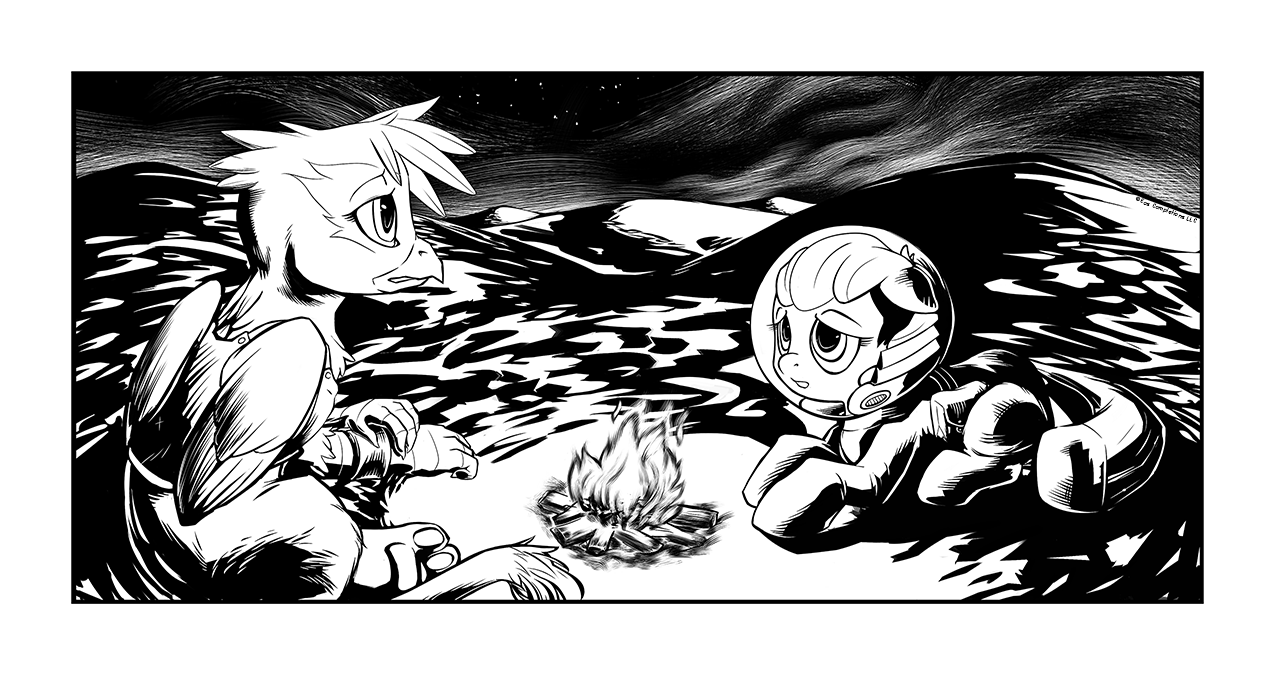
\includegraphics[width=0.9\linewidth]{image10.png}

\begin{intro}
在沙漠之中你要铭记自己的名字,因为没有一位马不会给你带来伤害。
\end{intro}

\daytimeplace{9}{2:00 AM}{太阳城市区,52号国道中段}{Sun City Downtown, Big 52 SC Branch}

「肏你妈,老娘头疼得都睡不着……」赫瑞塔揉着她的脑袋,帕比丢石头的时候不但瞄得挺准,而且力气也不小,现在狮鹫正在为帕比长时间锻炼的丢石头技巧埋单。在一整天的繁重体力劳动,比如拆房子,搬砖头啥的之后,狮鹫已经累得足以倒头就睡了——如果她的脑袋没有隐隐作痛的话。

「下次我见到那个黄色小恶魔的话,我要打她屁股打到她坐不下去。」说起来,那小东西在太阳城做什么?这个城市就是个陷阱,那个嗡嗡的洗脑声……

赫瑞塔一瞬间睁大了眼睛,「等等……那肏狗的嗡嗡声……没有了?老娘终于可以正常思考和喷脏字儿了!」半鹰站起来张开了翅膀正准备离开,但是下一瞬间看着她的几个室友呆住了,这个房间里有五只狮鹫,其中两个是一路把她追到这里的鹰爪,另外三个也纹着鹰爪的纹身,但是没有穿制服和铠甲。

「终于轮到老娘的复仇回合了……」赫瑞的喙上浮现出一个冷笑,然后拔出自己的匕首。她慢慢朝一只熟睡的狮鹫逼去,那只狮鹫既没有铠甲也没有武器,和她一样因为一整天的繁重体力活而睡得死死的。年轻的狮鹫像是草丛中的蛇一样无声无息地接近她的猎物,慢慢举起她爪子中闪着寒光的凶器……然后这个复仇者看到了那个狮鹫怀中的蛋。

「日你老母的……」看到紧紧抱着两个蛋熟睡的狮鹫,赫瑞塔眼眸之中的复仇怒火熄灭了。狮鹫迟疑着,她并不忍心杀死一个熟睡之中的母亲……但是另外四个就是……

另外四个又怎么样呢?他们也是这里的牺牲品,其中之一还可能是这些蛋的父亲,而且他们现在手无寸铁,还在熟睡之中,就算追着她的那两个狮鹫醒来,她也早跑到几公里之外了,在这里流血又有什么意义呢?

「肏你妈,老娘才不是背后捅谁刀子的懦夫……」赫瑞塔转身走向门口,不过她注意到屋子角落的一个粉色东西。是叫什么来着?丝袜?马尾啥的……反正是那家伙的玩偶。淦,差点忘记带上这东西,「哦,我了个擦!帕比!」她差点忘记带上那个死小孩儿!

\horizonline

\daytimeplace{9}{2:30 AM}{太阳城中心,52号国道中段}{Sun City Downtown, Big 52 SC Branch}

坐在漆黑的控制室里面,帕比依然不明白发生了什么,她完全不知道在声音先生回来之前,那个雌驹的声音是什么,不过她很确定那也是个漂漂马。不过只要想想那个可怕母马的声音在她脑中回响的感觉,就让帕比觉得不寒而栗。

不过很幸运,帕比现在状态很好,不管那个雌驹的声音干了什么事,最重要的是,先给她起个好听的名字,不过声音小姐已经用过了……

「啊……她就是她,小姐就是小姐,不过她就有点……呃……吓马?所以……鬼音?听起来好奇怪……」帕比皱了皱眉头,这个可真是个难题。「头音?不对……梦魇之音?太长啦……我知道了!怕音,因为她怕怕!耶!」

头盔的HUD上闪过一条提示,告诉帕比,任务:『梦魇现身』已经完成,没错,帕比太厉害了!她无所不能的!起个名字这种事情当然难不倒她。不过这么老长一段看不懂的字还是有点挑战性……而且数数超过自己的蹄子数量也有点儿……而且打开花生酱瓶子也……基本是不可能完成的任务……不过没关系,到现在为止她基本遇上的都是简单模式,所以出发吧!帕比!

好了,给自己打气结束,计划第一部分也完成,现在是计划的第二部分,找到赫瑞,然后像落叶赛跑中的小马一样快跑离开这里。

「好咯好咯!声音先生,赫瑞在哪?」

「{\mt 赫瑞塔·火红已经被设定为主要目标。}」

罗盘上的箭头消失,然后出现在帕比左边,箭头旁边表示距离的数字则快速的减少着。

「耶!冒险时……」

乒!

咣当!

乒!

一扇窗户被打碎的同时,年轻的飞行员拍打着翅膀,双爪紧握两把.45手枪,在飞溅的玻璃碎片之中冲进控制室。「坚持住帕比!」狮鹫在半空中两枪打碎了在EMP冲击之后刚刚恢复的灯泡,然后在一片漆黑中一个前滚翻躲在了桌子后面,这一连串的动作一气呵成。

突然出现的精彩表演看得帕比脸上露出惊讶的表情,哇塞,酷毙了!赫瑞绝对是最厉害的小马!简直就像电影中出来的英雄一样!小小雌驹在地板上踏着前蹄为她的朋友喝彩:「呀呼!冲啊赫瑞!你好厉害!太漂亮了!」接着一连串的子弹差点打中帕比的头盔。

「你丫干啥呢帕比,给老娘趴地上!我来解决那些肏蛋货!滚出来啊吃脑子的混蛋!」

「啥?」小雌驹一脸不解地歪着头。

发现这个屋子完全没有还击的对手,赫瑞尴尬地笑着,停止了扮演突击队员的角色,把枪放回枪套,用爪子按了按头顶的羽毛,想让自己看起来比较酷。

「嘿,帕比,没缺蹄子少尾吧?」

幼驹低头数了数自己的蹄子和尾巴,然后点了点头,「我都带在身上呢!丝尾没事吧!」

「你的玩偶?哦,你想要吗?」赫瑞拿出粉色的毛绒玩具晃着,而帕比摇了摇头。

「才不要咧,她和你在一起很好,我让她看着你,她还警告我说你有危险,所以我来这里救你但是你做着鬼脸骂了我然后又不理我所以我等到入夜之后执行我的超绝密潜入计划去告诉镇长这镇子烂透了但是我来到这里之后发现镇长不是镇长而是个傻蛋声音还说我的坏话但是我比他聪明所以他说很抱歉然后跑掉了,所以——我比蓝声音聪明!\footnote{这里类似于S01E12里苹果丽丽对云宝黛西说话的语速,节奏也一样}」

赫瑞塔举起一只爪子:「等等等等等!你他喵的嘴动那么快老娘一个字都没听清都就听你吧啦吧啦!都什么乱七八糟的,而且也没那闲工夫听你逼逼,赶紧麻溜地过来,这地方现在挤满了英克雷的杂毛和鹰爪的狮鹫,还有不知道天杀的什么势力的马——全都坐在一大堆新鲜食物和干净的饮水上。」

帕比疑惑地玩着头,「呃……那么,然后呢?」

狮鹫无奈地用爪揉着脑门,「好吧,长话短说,几小时之后这里就要变成个大战场了,在此之前我们要赶紧溜号,懂?」

「战场?就是小马们互相伤害的地方?」帕比有点疑惑地问。

「对,你丫可算是对了一回,每堆小马都想要把好东西全都占为己有,所以赶紧把口袋里没用的死重的东西都丢了,在被炸上天之前要赶紧飞离这个火药桶。」

帕比皱着眉头,「但是为什么要争斗,小马应该是漂漂而且好好的,打架是不对的,我们要爱与宽容……」小幼驹说着她的简单生存理念。

赫瑞塔正想反驳说就是这爱与宽容把小马国变成现在这么个大粪坑,但是她也明白这可不是和帕比斗嘴的时候,「对,没错,但是在你丫被『爱与宽容』之前还是快点闪……呃……你不是还得找你妈妈么?」

帕比点了点头,「对啊!我要去那个什么天麻肥鸡场什么的地方,但是漂漂姐姐和我说那里叫……啊……我不记得名字了,不过罗盘上有个箭头我绝对不会错过的!」

赫瑞塔叹了口气,「我猜,这地方在天杀的南边吧。」狮鹫伸出爪子指着。

帕比惊讶地看着她的朋友,「哇哦,你怎么知道的?你是魔法师么?」

「没错,老娘可是小马国最伟大的魔术师,天下无双的赫瑞……现在赶紧的!把你的破烂都倒出来。」狮鹫顿了顿,然后看着她朋友问,「话说,你什么时候给鬃毛染了个蓝条?」

一缕蓝色的鬃毛在帕比额前闪闪发光的金发之中格外显眼,就在她右眼上,这道鬃毛看起来就像是一道夜空的剪影一般,让赫瑞塔想起来自己见过的那什么魔法部的招贴画,那个叫暮光傻傻还是什么的家伙。

\horizonline

\daytimeplace{9}{3:00 AM}{太阳城中心,52号国道中段}{Sun City Downtown, Big 52 SC Branch}

帕比大着胆子睁开一只眼睛看了看下面,地面在夜空中飞快地向后滑去,高大的大厦看起来就像是火柴盒一样,布满灰尘的公路就在她鼻子下面快速地移动——不过距离她鼻子实在太过遥远到让她不舒服。

「我我我我我们还没到吗啊啊啊!!」小雌驹用力抱紧赫瑞塔的脖子,狮鹫觉得自己快要被掐死了。

「呃!松开你丫的蹄子!想让老娘陪你一起坠机么?」

一开始带着帕比飞还很顺利,这个小家伙丢掉身上的垃圾之后,重量还不如一个背包沉。可是当帕比发现她恐高之后,麻烦就开始了……{}

「你就闭上眼睛,当做自己是在骑小马啥的!」

帕比把自己眼睛闭得就像是避难厩的大门一样,但是完全没有用,一想到那些房子,树木啥的飞快地移动得就像是一团模糊的水彩一样,帕比就……「拜托,拜托!拜托我会做个乖孩子!放人家下啊啊啊啊啊!」

「我勒个擦,你丫至少对你朋友的飞行技术有点信心好不好!」赫瑞塔用力拍打了一下翅膀,然后从两座高楼之间的缝隙穿了过去,远远离开太阳城,清凉的夜风带着海水的味道,今晚绝对是个飞行的好夜晚——如果没有背上这个吵闹的包袱的话。

「你丫给老娘放松点儿!可以唱点歌什么的嘛!」

唱点歌,帕比觉得这个意见听起来不错!只要唱个歌一切都会好起来!小雌驹清了清嗓子然后开始唱。

「
\begin{song}
    蛋头蛋头坐墙上
    
    蛋头蛋头摔地
\end{song}

……啊啊啊啊拜托拜托拜托拜托拜托放!人!家!下!来啊啊啊啊啊!」

作为一个狮鹫,一个掠食者,在她远古的血液中,赫瑞是很高兴抓着一只在她双爪之中挣扎的小马猎物,但是一个在她脑袋上跳舞的幼驹就是另一回事了。「你丫给我安静!不会让你掉下去的,所以别惹老娘发火!……也别扯毛!你这死丫头知道背上的羽毛长回来要花多长时间吗!?」被帕比惹火的年轻飞行员把小雌驹从背上甩下来,然后用前爪紧紧抓住。「这回至少不会掉下去了!飞出废墟就给你放下。」

「咿……呀……!」

「小鬼别尿裤子,还要飞几公里呢,我们最好在那个大号火药桶炸上天之前离开这地方。」半鹰兽说着加快速度,用尽全力拍打着翅膀,她们俩就像是『嚎哭女妖』一样划过夜空,惊醒了沿途的所有小马,赫瑞塔祈祷着没有小马探出头寻找声音的来源。

\horizonline

\daytimeplace{9}{3:30 AM}{蛇蝎沙漠,52号国道中段}{Serpent Desert, Big 52 SC Branch}

「其实人家一点也不害怕,你懂的……只是……只是那啥……呃……看着那么多房顶,吹着风,然后有点……嗯……稍微有点兴奋……尤其是不知道你往哪儿去的时候。」四个蹄子都接触到了结结实实的地面之后,帕比正在为了挽回自己的面子而拼命辩解。不过从赫瑞塔笑得满地打滚的状态看来,这努力完全没有效果。

「活宝,你真是个活宝!」狮鹫在狂笑声之中吸了一口气,擦了擦眼泪,然后又爆出另一阵大笑。「你怎么尖叫的?咿……!再来啊,再叫一次我听听!」

黄色的小雌驹噘着嘴坐在地上叹了口气说:「哼,是谁在这城里迷路啊……小鸡你真是……」

乒……

帕比低头看着她黄色外套上胸口位置的一个大洞,喊了起来:「我说,那么多坏机器打我还不够啊?!」

赫瑞塔毫不在意地在爪子上转着自己的手枪,依然止不住刚才的大笑,「抱怨个屁啊,你丫给蝎尾狮扯成碎片都没事,老娘再给你开俩洞又能怎样?」

乒!乒!

又有两发子弹穿过帕比,一发打在蹄子上,一发打在胸口,「别闹了好吗!每次衣服有洞这破衣服都会念叨个没完!」在狮鹫打出的洞上露出了一丝粉色的气体。

「好吧,不过丫的别叫老娘小鸡好吗?」打了个哈欠,赫瑞塔收起了手枪,「顺便提醒你,普通小马甚至尸鬼被子弹开个洞都会死……所以别和其他小马玩这个游戏,好么?」

帕比点点头,然后又有点疑惑地歪着头,「但是我也是个普通小马,我是小马!」

「喂喂,我说你不是……喂,怎么忽然这个表情了?你是想让我唱个摇篮曲么?」赫瑞塔一脸调侃的表情问。

小雌驹开心地点了点头,「当然!我超超超超超爱摇篮曲!我们可以一起唱《静悄悄甜蜜蜜》吗?」

狮鹫一脸不爽地以爪覆面,该怎么才能告诉这个小雌驹她只是在调侃而已,「你真是麻烦,帕比……」

\begin{song}
「静悄悄,甜蜜蜜,该是安睡的时间!


\begin{englishlyric}
    ``Hush now, quiet now, it's time to lay your sleepy head!
\end{englishlyric}

\medskip

静悄悄,甜蜜蜜,还是入眠的时间!」 \footnote{这是正剧S01E17中的歌词}


\begin{englishlyric}
    Hush now, quiet now, it's time to go to beeed!''
\end{englishlyric}
\end{song}

赫瑞叹口气继续往南走,「为什么,老爹啊,老娘怎么就欠了这个傻蛋两次!」然后她笑着回过头说:「你坐上你的红滑板车吧,我在你头上飞,如果你想明天之前到那边的话,我们还有很多路要赶呢。」

\horizonline

\daytimeplace{9}{10:30 PM}{蛇蝎沙漠,52号国道中段}{Serpent Desert, Big 52 SC Branch}

帕比和赫瑞塔围在小小的营火边,她们的影子落在远处的沙丘上,赫瑞塔正在吃着一个锡罐里面的食物,从她的表情可以看出那东西显然不适合狮鹫的饮食习惯。沙漠上空的厚厚云层让这里在夜间也很温暖,但是那个半鹰依然穿着她的铠甲。

「这么说,那个蓝声音什么的说你是机器?」

赫瑞的表情看起来有些微妙,似乎是想在幼驹说完整个故事之前努力保持一副扑克脸。

「对,而且他听起来非常确定……我差点也信了,但是另一个怕音告诉我那是不可能的,因为……呃……我不明白她说的到底是什么,不过听她说的话应该没有问题。」帕比睿智地点了点头,就好像她什么都懂一样。

狮鹫耸了耸肩,「那么说,一个电脑说你是某种疯狂机器马,然后又有个幻觉说你不是……我觉得你肯定是被那EMP弹震晕了,然后EMP残存在你防护服电路里面的静电让你做了一个噩梦。」赫瑞塔打了一个哈欠,继续说:「不过我可不觉得你是机器……机器挨枪子儿会爆炸……而且,机器聪明多了。」

幼驹皱着眉头,「那你觉得我是什么?」

半狮子蹲坐在地上抓着自己的后腿,「你?反正对于我来说你不是啥好事……不过我喜欢你,所以你可以跟老娘混,叫『大姐姐赫瑞』。」

帕比走到她伙伴面前,直视着赫瑞塔双眼,幼驹的双眸在夜空中就是两个亮亮的粉色光源。「哦……但是……我是小马,对吧?我是说,就算我不吃东西不喝水而且还不上厕所,但是我还是小马?对吧?我是小马吧……」

\emph{她看起来忧心忡忡的样子,这个机器马什么的事情看起来真的吓到她了,不过……真他喵的肏蛋,为啥是老娘收拾烂摊子?}赫瑞现在完全精疲力竭,最不想见到的就是个打破砂锅问到底的幼驹,她现在只想要睡觉。哈欠连天的狮鹫拍着幼驹的头盔,「你是什么都不重要,帕比,你是个善良的小马,在废土上善良的小马很难见,只要你还认为自己是小马,你就是小马,所以……睡觉吧,拜托。」

幼驹开心地笑了。隔着头盔蹭了蹭赫瑞塔。

「谢谢你赫瑞,你是我最好的小鸡朋友!」

坐在她熟睡的伙伴身边,帕比叹着气,她一点都不困……

……

……

「喂!你说我因为机器很聪明所以我不是机器是什么意思!」帕比生气地戳着狮鹫的屁股,但是赫瑞只是轻笑一声然后转过身去。

「活宝。」

小马不停地戳着她的朋友想要听到回答,但是狮鹫开始大声打起了鼾,留下无奈的帕比独自坐在快熄灭的营火边。

\daytimeplace{10}{1:00 AM}{蛇蝎沙漠,52号国道中段}{Serpent Desert, Big 52 SC Branch}

寂静的黑夜之中帕比毫无倦意,幼驹一点都不觉得累,但是赫瑞现在不想被打扰,所以幼驹做了她自己觉得最合理的事情,在沙漠的夜晚上放哨,因为帕比最聪明了!

不过这里和帕比的期待根本对不上。那么多牛仔电影里面,沙漠应该都是骷髅,箭头,风滚草还有各种乱七八糟的东西,但是在『真正』的沙漠之中走了几天之后,帕比觉得那些水牛估计都休假去了,而且这里一只蝎子或者蛇都没看到,怎么可以叫蛇蝎沙漠呢?她目所能及之处只能看到几辆马车的残骸,还有一个看起来像是大号贪吃灵之类的东西在不远处闲逛,不过她靠近的时候,那些贪吃灵为了躲避她都飞走了。

「{\mt 警告,发现敌对生物。分析中,变异贪吃灵。威胁等级:致命。}」

「哎,为什么这里所有的毛茸茸生物都这么害羞?我只想交个朋友!」活了两百年的老怪物对着自然母亲和污染父亲联姻突变的小怪物说。

「嗨帕比,好久不见,你可真是跑了好远啊,不是吗?」一个金属的声音打断了小幼驹的小小探险,小可爱开心地笑着转向她的朋友。

「提问者先生!你去哪里啦?」

「是守望者,我守望着废土,守望……」

「好啦好啦,提问者先生,」帕比点着头微笑着,「我也可以守望什么吗?」

机器精灵发出金属质的窃笑,「帕比,帕比从未改变\footnote{这里改编自 \emph{FoE: PH} 的名句「战争,战争从未改变」}……你最近还好吗?我听说你在隧道镇有个小小冒险,而现在你已经跑到太阳城南边了。」

「没错!见到了好多漂漂马!有个叫赫瑞的小鸡,还有阿索和甜花,乐乐姐,还有好多好多朋友!」

「哇哦,你有这么多朋友,真幸运,不是吗?说起来,你去太阳城了?」声音想要保持一个稳定的音调,但是却透出一股好奇。

帕比皱了皱眉头,「对啊,就像一个用丝带包着的超级棒的礼物盒,但是里面却塞着燕麦……大家都一脸不开心,而且不和我聊天不和我玩,他们的镇长是个笨声音只会说可怕的话。」

「什么可怕的话?你想和我说说看吗?」

守望者的声音现在听起来很担心。

帕比看着远处说:「他说我不是小马是机器,然后我用那个可以让机器睡觉的大茶壶让他睡了,但是我也不能动……大家都说我不是机器,但是为什么……」

「呦呦,帕比,别烧坏你的小脑子,我可以很确定地说你不是机器,那个声音估计读取了一些感应器数据,但是它只是个看不懂小马心灵的机器,你也是个漂漂马,懂吗?现在对我笑笑,别再去想咯。」

帕比点点头,轻轻地笑了。

「非常好,满城的僵尸马……你找到什么发出兹兹或者类似轰鸣声的东西么?」

「没啥,但是赫瑞和我说那个吱吱声已经消失了,所以那些漂漂马会醒来然后做不漂漂的事情。」

「哦,终于那自律智能不见了,我终于可以看看里面……我想,又是你做的吧?」

帕比皱了皱眉头,「不,我只是听说赫瑞有危险所以过来……但是她没有,而且像个傻鸡一样飞来飞去不理我,和城里其他小马一样,所以我去找镇长声音和她吵了一架,然后他说我是傻瓜于是我拿出蓝色大茶壶……」

「呃……抱歉,蓝色大茶壶是啥?」

幼驹叹了口气,用蹄子扶着头盔,「为啥我每次都要从头解释?就是一个茶壶,圆圆的,亮亮的,还有个蓝色尖头!我在一个沼泽的破烂车车里面找到的!」

「好吧,所以你在一台超级计算机面前引爆了一个EMP震荡弹,的确,搞定那自律智能的又是你……话说你鬃毛怎么了?」

帕比歪着头想要看自己的鬃毛,「你说那个蓝条?我不知道,我一醒来就……」

「嘿帕比,那是谁?我就来!」赫瑞的声音打断了小马。

「抱歉小家伙,我要走了,你下次可以和我讲这个故事。」不等她回答,机器精灵发出一阵静电啪啪声,就继续开始播放音乐了。

狮鹫双爪各持一把枪落在沙丘上,不过她发现这里没什么威胁之后,双枪少女收起武器训斥着帕比,「坏孩子!别和机器精灵玩儿,回营地来。」

帕比和漂浮的机器挥了挥蹄子,然后回到了她朋友身边,「我没玩儿,我只是和他说我的超级大冒险!」

「对,对,对,我们回去睡觉吧,明天还要走很远呢。」狮鹫揉了揉帕比的头盔然后回到营地。

一个半小时之后,吓坏的肉食灵终于从隐蔽之处出来继续建造它的巢穴。

\horizonline

{\rt 雌驹们,公马们,早上好!这里是孤狼的52电台!你敢说废土还有比我这里更好的电台么?谁?DJ PON-3?拜托,我听说他只是个雌驹,不骗你们,而且在晴朗之夜她还会变成三头钻石犬!我不骗你们,只要在晴朗夜晚去十马塔就能看到!不过L.P.我很确定废土不会有什么晴朗之夜,或者晴朗之日。不过这不是我的错小马们,你们继续听52电台,别管什么DJ了!

好吧,回到新闻时间!昨天早上太阳城从19年的长眠之中醒来,我不知道具体发生了什么,不过看起来在晚上有谁袭击了城市的中央控制塔,摧毁了不知道谁放在那里的洗脑电台。没错小马们,你们没听错,以前太阳城是不归之地是因为那里完全被洗脑电波控制了!简直是疯狂!

你们猜那些住民意识到洗脑电波结束之后他们干了什么?你没猜错,他们开始继续相互残杀企图夺取城镇,如果你想穿过蛇蝎沙漠,跟着东边的绿色路径绕道,远离太阳城,重复一遍,尽可能远离太阳城!

好吧,大家可能还要问,谁是撤换城市管理员的家伙?还用得着我说那个名字吗?没错,伙计们,我们的小小英雄把你们从永无止境的噩梦中拯救出来,而你们还把你们的生命继续浪费在互相杀戮这种无聊的事情上!你们还有廉耻没有?我……算了,不提也罢,我们还是听会儿音乐吧。

现在即将播放的是:永不可及……}

 DJ的声音被音乐代替。

\begin{music}
看着你的孩子争斗。

\begin{englishlyric}
    Look at you young colts fighting.
\end{englishlyric}

\medskip

看着你的女儿哭泣。

\begin{englishlyric}
    Look at your fillies crying.
\end{englishlyric}

\medskip

看着你的儿女死去,

\begin{englishlyric}
    Look at your young colts dying,
\end{englishlyric}

\medskip

正如往昔一样。

\begin{englishlyric}
    The way they've always done before.
\end{englishlyric}
\end{music}

\horizonline

\daytimeplace{10}{10:30 AM}{铁锈庄园,52号国道中段}{Rust Manor, Big 52 SC Branch}

铁锈庄园看起来和它的名字一模一样,不知道是谁用巨大天空马车残骸建造了一个超级大号的路障,在不远处可以看到屹立在沙漠之中的兵营和空管塔,整个建筑都被强化钢板覆盖着,但是现在所有的金属都被锈迹侵蚀,看起来这里严重缺乏维护。不过,此地只是个小小的交易站,几辆篷车就在小镇外面,北边的大门附近有很多卫兵在地面和城墙的塔楼上巡逻。

远在几公里之外,赫瑞塔就叫帕比停了下来,毕竟在战争期间这里也是个军事要塞,不过这里的建筑除了空管塔楼基本都被炸毁了,所以这里的一片空地非常适合塔楼上的狙击手控制整个区域。

「等等,红箭!」狮鹫降落在小雌驹面前,让她在一团烟尘之中刹车。

「哇啊!看好降落地点啊!我差点撞上你!」

「我知道啦,好了,你丫这个鱼缸脑袋仔细听好,我现在要走了,不过这里很安全,你不会有麻烦的。」

帕比睁大了水汪汪的眼睛哀求着。「为什么?我不想你走啊!」

「我知道,我超酷的,没有老娘你丫啥都不是,不过那些在太阳城追我的家伙估计已经在这里等我了,我不想把你卷入麻烦。」

「哼!如果有坏小鸡追你,我们可以和他们解释你是个好孩子,然后和他们道歉他们就不会惹你了吧。好么?」

赫瑞塔叹了口气拍了拍帕比的头盔,「故事比你想象得复杂,毕竟我爆了他们好几个伙计的脑袋,所以他们现在在追我,所以……没戏,我可不觉得我们道个歉就能解决问题,而且我也不想道歉,他们杀了我父亲。」

「哦……」帕比低下头,想着其它解决办法,「你不能欺负那些欺负你的孩子,我是说哦,他们不是坏机器,他们是漂漂猫,你不能欺负小猫猫!」

赫瑞塔嗤之以鼻,「没错,漂漂猫……所以我不想进城,如果我不进去,我也没必要去把他们揍到不能再欺负我为止。」狮鹫耸了耸肩,「不管怎么说,照顾好自己,帕比,我们很快会再见了。」不等帕比回答,赫瑞塔就在一阵沙尘之中飞上了天空。

幼驹追着她的朋友跑了几百米,大叫着她,「唉,这不公平,她都没和我吻别……」幼驹看着天空尖叫着,「丝尾,照顾好她,她现在归你负责啦!」

\horizonline

\daytimeplace{10}{11:00 AM}{铁锈庄园,52号国道中段}{Rust Manor, Big 52 SC Branch}

狙击手在瞄准镜之中看着那个黄色的点,但是独角兽雌驹不太确定她看到的是什么,于是她把蹄子按在了对讲机上,「这里是坚守,一一八六处有情况,看起来是一个穿黄衣服的小马,或许是无线电里面说的小幽灵,看起来很像……我们这里欢迎幽灵么?」

对讲机传来了回复:「继续注意目标,如果你看到敌对举动再报告,否则让她继续靠近。」

「了解!」雌驹回到她的守备位置。

同时,帕比来到了前面,引起了大门外所有卫兵的注意,很多小马都相互窃窃私语着,举起了武器。不过小雌驹完全没有留意他们的举动,她只知道妈妈或许在那个镇子里面!

「嗨!我是快乐帕比!你们看到我妈妈了么?声音先生说她在这里!」

所有的小马都看着小雌驹,然后其中之一叹了口气,「没错,这个就是孤狼说的小幽灵。」卫兵放下他们的武器继续各忙各的去了。不过没有小马回答她的问题。

「呃……我想,你们是说没有吧。」幼驹一脸狐疑,发觉自己再次被忽略,于是她喃喃自语着:「求马不如求己,好吧声音先生,我们该去哪儿?」

「{\mt 分析中,读取本地地图,蓝羽机场,无法匹配,读取备份资料,寻找可能地点,地点找到:中央控制塔。中央控制塔被设定为下一个目标点」罗盘的箭头开始转向。}」

「哦,在城里!好!」帕比转头走向大门,但是马上被一个穿着雇佣兵铠甲的老公马拦住了,他眼中的神情帕比觉得很熟悉,她想起来曾经见过这一幕。

\rcpr{「喂喂,妈妈,为什么那个小马只有三条腿?」}

\rcpr{「她是战斗英雄,帕比,别打扰他,他已经很累了。」}

\rcpr{「说得没错,把我的腿献给破烂女神的破烂敌人,老子不知道那些破烂煤值得那么多小马去死么?」}

\rcpr{「哦……漂漂马说了奇怪的话!」}

\rcpr{「帕比,别听他胡说,那些都是坏话!你也是,和一个小孩子讲粗口害不害臊?」}

\rcpr{「滚边去婊子……」}

\rcpr{「我们走吧,帕比,跟我来,」}

\rcpr{「但是妈……我想要……」}

\rcpr{「死粉老鼠,找你妈哭去!没啥好看的!」}

帕比眨了眨眼,沉浸在回忆中,当她回过神来的时候,那个愤怒眼神的老马依然站在那里,小雌驹战战兢兢地走过去,「嗨……你见过我妈妈么?」

佣兵啐了一口,「你聋了?」

幼驹坐下来,有些疑惑地看着骂她的马,「呃……很抱歉我没听到你说什么……为什么你那么生气?我做错什么了吗?」

雄马轻蔑的笑着,「我问你丫是不是觉得自己是个英雄啥的?」

帕比微笑起来,这个问题简单。「我是太空战士安德洛队长!只要有我的太空服和超快飞车,我可以跑遍整个世界交很多很多好朋友!想和我玩么!我还有一个火箭!」小雌驹举起蹄子说:「火箭!」一个火箭玩具飞到了小雌驹面前。

老马抬起一根眉毛。「你把我当傻子吗?你知道老子是谁么?别在这里装逼,找肏是不是?」

帕比咯咯笑着,奇怪的话总是逗她笑,「哦……漂漂老马说奇怪的话了,我能一起玩吗?我会造词!比如说,滑板爪子!或者香蕉电话!」

那群小马开始大笑起来,小雌驹不知道他们在笑什么,不过她也一起跟着笑起来……不过这样下去迟早某马会血溅沙漠。

坚守又一次把蹄子按在对讲机上,「坚守报告,北门外面的佣兵队有麻烦了,那黄色小马看起来要和佣兵打起来了。」

「我们派卫兵去解决,在我们没有被攻击之前不要轻举妄动!」

「收到!」

这时老马抓着帕比的蹄子把她拎了起来,凶恶地看着她,「你刚嘲笑老子?就是因为电台里面的傻货吹嘘几次,你丫是不是觉得自己天下无敌了?」

「喂,放下我,我要找我妈妈!我又没惹你,大坏蛋,放我下来!」幼驹挣扎着,但是却没法挣脱,「我妈妈如果在的话她一定会教训你的,放开,放开我!」

或许是孩子的哭声让紧张的气氛消失了,那群小马有些尴尬地别开了脸,那个老佣兵也不知道自己到底在干啥,这个小丫头不是什么看起来超级厉害的英雄,穿着闪闪发光的骑士铠甲在城市间执行什么只有露娜才知道的神圣任务,她只是个……「肏蛋,孤狼绝对是脑子进了水才会觉得这个智障儿童是个英雄。」

这时候帕比开始哭了,哇哇地大哭,没有小马想去看这么没面子的事情。

佣兵叹了口气把幼驹放地上,「滚边去,老子不打小孩。」他轻哼一声,帕比转头哭着跑掉了。

在内心深处,他觉得自己也像是个坏蛋,而且为此而羞耻不已,不过那也只是一瞬间罢了。

~\vfill

\begin{note}
升级(Lv 9)

新技能解锁:哭泣公主——你可以用哭泣来解决几乎所有问题,你可以解锁特别对话选项来避免战斗,不过你会因此而损失声望。
\end{note}




\chapter{家族涂鸦}

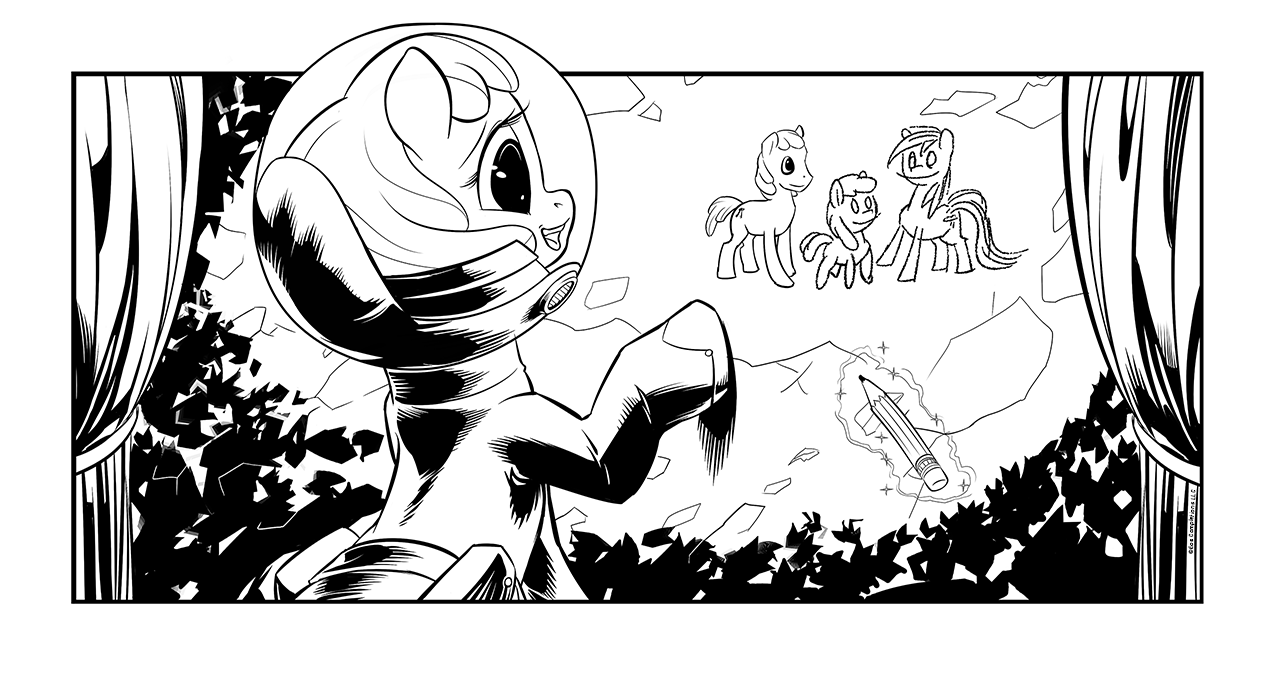
\includegraphics[width=0.9\linewidth]{image11.png}

\begin{intro}
你没有用电动工具,对吧?
\end{intro}

\daytimeplace{10}{1:30 PM}{铁锈庄园,52号国道中段}{Rust Manor, Big 52 SC Branch}

{\rt 嗯哼,大家下午好,这里是孤狼的铁锈庄园特别新闻!}

在噪杂的背景声之中可以清楚地听到一个女性的声音,然后有谁在叫着『你个老巫婆给我让座!』还有一阵金属撞击声。

{\rt DJ好货在新闻之后马上回来,我要说,什么叫好货啊,你在干什么,那是铁桌子,哦,哦,哦别!我对你够温柔的了,好吧,你自找的,尝尝我的爱与包容吧!}

在一阵被按住嘴的声音打断了放送之后,孤狼终于喘息着回到麦克风面前。

{\rt 代表好货祝你们健康,她很快回来,在她解开蹄子上的电线……好吧,我们还是来说我们的特别新闻!这个是来自一位铁锈庄园的电台同好!感谢小蝴蝶23!}

孤狼清了清喉咙然后继续往下讲。

{\rt 有些英雄倒下了,有些英雄被杀害了,有些英雄消失在避难厩中再也没回来……不过,我们的英雄被打屁股了,对,你没听错。在早上早些时候,小小幽灵在铁锈庄园外碰上了一队雇佣兵。一个卫兵当着很多小马的面骂了她。好吧,你这家伙脑子抽了么?我们知道这个孩子摧毁了赤兔领土上的那个农场,然后冲进重兵防守的隧道镇,那里的快乐扳机说她看到那个幼驹单枪匹马用一个石头砸坏了六个哨兵机器……但是你呢,你和一个小幼驹打架?你活得不耐烦了?就算现在你看起来打赢了那个小孩子——如果你管那叫做『打架』的话,在我看来不过是一个可爱的小雌驹想要对你示好却被你欺负得哭着跑开!}

然后是一阵长长的叹息。

{\rt 这就是所谓的感恩……L.P.播报结束,在好货回来之前先听点音乐吧,我先逃命了。保持优雅,52国道。}

然后是一阵音乐声。

\begin{music}
看着你步出一零零九房间

\begin{englishlyric}
    Saw you stretched out in room Ten O Nine
\end{englishlyric}

\medskip

你笑颜如花,却又泪眼潸然。

\begin{englishlyric}
    with a smile on your face and a tear right in your eye.
\end{englishlyric}

\medskip

那模糊的心意宛如雾里看花,

\begin{englishlyric}
    couldn't see to get a line on you,
\end{englishlyric}

\medskip

我甜蜜的爱侣啊。

\begin{englishlyric}
    my sweet honey love.
\end{englishlyric}
\end{music}

帕比躲在一辆废弃的卡车后面,依然抹着泪。这次她又做错什么了,她真的很努力去做一个好孩子,但是所有的事情看起来都和她对着干。从那个疯狂的派对机器马和房顶砸在头上开始——她就是块会吸引噩运的磁铁。妈妈为什么一直跑来跑去不等她?小小雌驹觉得又累又空虚。

\begin{music}
斑马的珠宝洒落在街上,

\begin{englishlyric}
    Zebra jewelry jangling down the street,
\end{englishlyric}

\medskip

你闭上眼睛,封闭心灵之窗。

\begin{englishlyric}
    make you shut your eyes at every filly that you meet.
\end{englishlyric}

\medskip

那冰封的心中仿佛风雪飘扬,

\begin{englishlyric}
    couldn't seem to get a high on you,
\end{englishlyric}

\medskip

我甜蜜的爱侣啊。

\begin{englishlyric}
    my sweet honey love.
\end{englishlyric}
\end{music}

但是帕比不能就这样坐下放弃!就算长路漫漫没有尽头,她的妈妈一定在山另一边的某处,或者就在下一座山后面,一次翻越一座山,总会找到妈妈的!

\begin{music}
愿公主为你降下一缕阳光,

\begin{englishlyric}
    May Celestia shine a light on you,
\end{englishlyric}

\medskip

优美的歌为你唱响。

\begin{englishlyric}
    make every song your favorite tune.
\end{englishlyric}

\medskip

愿公主为你降下一缕阳光,

\begin{englishlyric}
    may Celestia shine a light on you,
\end{englishlyric}

\medskip

温暖如傍晚的夕阳。

\begin{englishlyric}
    warm like the evening Sun.
\end{englishlyric}
\end{music}

黄色的小雌驹站了起来,在车子后面哭鼻子可没法找到妈妈,她是肩负重任的好孩子,不要在意那些小事,前进吧帕比!

\horizonline

\daytimeplace{10}{1:45 PM}{铁锈庄园,52号国道中段}{Rust Manor, Big 52 SC Branch}

在大门站岗的两个卫兵快速对视了一眼,看起来不确定该由谁应付这个走过来的幼驹。终于比较大的那个说话了,「抱歉小鬼,如果你想进去的话,你应该付钱,两百个瓶盖,还要把你的武器放在这里。」

帕比皱了皱眉头,两百对于她来说是个超级大的数字,她可以用自己的蹄子数到四,说不定还能数到十,不过两百?一百是多少?

「呃……我只是在找妈妈,超超拜托……」

「拿出你的瓶盖就行了,小孩子。」卫兵打了个哈切,想要保持冷静,但是他担心如果小雌驹没有钱还要往里走的话,或许该是叫老大……{}

「袋子!」

一个超级大的袋子飘在了帕比面前,她交给了卫兵,「呃……你们能帮我数数看么,这些闪亮瓶盖够么?」

卫兵点了点头然后把袋子倒在桌子上,那里面一多半是瓶盖,剩下的都是站前货币,甚至还有一些金币,「没问题,这些足够了。」那个卫兵看了看另一个守卫,而后者满脸失望地哼了一声,「你想干啥,这么可爱的一个小雌驹,你不会是认真的吧!」

那个卫兵叹了口气,数了两百个瓶盖,然后把剩下的还给帕比,小雌驹开心地把自己的收藏品收了起来。

「漂漂卫兵超超超谢谢你们!」

在城墙里面,铁锈庄园又小又拥挤,天空马车的残骸不但用来建造城墙,还被当做房子和商店,只在中间留出勉强够小马通行的小路,帕比觉得这里就像是蚂蚁在树下面建的小镇一样——不过这里的『树』有近百米高。帕比在附近溜达着,时不时地偷瞄一下商店里面,想找条路走进高塔,箭头直接指向那个最大的塔楼,但是在这里找条路进去不容易。

街道上小马很多,有些本地居民好奇地看着帕比,不过他们都在忙自己的事情,把她当做一个没什么威胁的奇怪东西,尤其是在她『解决』那些佣兵之后。帕比也不在乎,至少她找到了一个真正热热闹闹的地方,而只要有成年马在的话,就一定会有……「耶!小马在玩!」

三只幼驹,一个小雌驹俩小雄驹正在跑来跑去。开心地大叫大笑着,看起来超级有趣!但是帕比应该去找他妈妈……不过她走掉的话,那些漂漂马……她现在想要玩的时候为什么不去玩呢……但是妈妈……或许玩个几分钟也没问题吧!或许可以问问他们见到过妈妈没有,顺便还可以交个朋友!没错,只是交谈,不是玩,和漂漂马交谈,就像妈妈经常做的那样,因为他们有可能知道妈妈在哪二!嗯,聪明的帕比,甚至比自己都聪明!

「嗨,我是快乐帕比,你见过我妈妈么?」

幼驹们停止了嬉闹,转头看着新来的孩子,他们之中有一个灰色粉鬃的小独角兽雌驹,另外两个小雄驹有一个很像这个雌驹,另一个是棕色鬃毛绿色毛皮的陆马,他们看起来都一些吃惊和困惑,然后小雌驹问道:「你从哪弄到这个超奇怪的太空服?」

黄色的雌驹皱了皱眉眉头,「这才不奇怪,这是太空战士安德洛队长服!」说到这里帕比做了一个经典的停顿来炒热气氛,然后她补充道:「超级酷!」

独角兽雄驹点了点头,「对哦,我有安德洛的漫画!她是个超级酷的姐姐!她有一把镭射枪来消灭斑马异形!」

另外两个小孩子认同地点了点头,独角兽雌驹露出友善的微笑,「我是政要,」然后指着那个独角兽雄驹说,「他是我的双胞胎兄弟跳弹,他是止痛。」

「我是快乐帕比,我来自中心城,现在正在找我妈妈……你们在做什么,在玩吗,一起玩吗?」嗯,重要的事情要问两遍,而且有时候她可以休息一下,爸爸妈妈们也需要休假的嘛。

跳弹歪着头问:「你妈妈?她叫什么?」

「她叫阴雨·黛丝,她是最酷的小马!她会做马芬和杯子蛋糕还有巧克力布丁和苹果派!不过她总是给我吃苜蓿……她几天前去工作,然后我们在中心城的家塌了,于是我到处找她,声音先生知道她在哪里,不管怎么说总比在房子的废墟那里等她要强……大概……?」

三个小孩子点了点头,好像帕比的演讲他们听懂了一样,「没错,上回我打碎一个瓶子妈妈气坏了,我不知道你妈妈知道你打碎整个房子的时候会气成什么样……」

黄色幼驹皱着眉头,「又不是我的错!我睡了一觉醒来的时候整个房子都不见了!」

「你妈会信嘛,上次我就想说是一堆奴隶贩子打碎的那瓶子,但是妈妈总有某种超自然感知能力知道是谁干的……」止痛跟着说,声音很小似乎不想让其他小马听到他的秘密。

「我绝对不想弄坏房子的!我可以发誓!」帕比坚持维护自己的正确性,不过最主要的还是房子坏掉的时候附近没有其他马在,不过她还是要坚持不是自己弄坏的!

「你最好别这么说……」政要打断她,「不过我没在铁锈庄园认识任何叫『阴雨·黛丝』的……对了,我们在玩牛仔和斑马游戏,要来玩吗,你可以当外星马!」

止痛不满意地说:「我可不想再当斑马了,你们俩为什么不当一次斑马?」

跳弹戳着他姐姐的角说:「因为斑马没有角呀!」

「我听说过斑马还可以用奇怪的装置长出蝙蝠翅膀!」帕比插话:「而且,我想当安德洛队长!」

「但是你又没有安德洛的枪……不过你可以当金盏菊\footnote{金盏菊(Marigold):这里作者写成 Maripony,但根据 \emph{FoE} 设定,战前靠火箭登上月球的小马宇航员应该是 Marigold},登上月球的雌驹!」跳弹说到一半就被她姐姐打断了。

「她从来没有登上月球!小马不可能去月球!」

「她上了!」

「她没上!」

「她上了!」

「她没上!」

「她上了!」

「她没上!」

双胞胎脸红脖子粗,鼻顶鼻,眼瞪眼地争吵着登月计划,止痛走到帕比身边叹了口气,「他们估计又要吵到吃晚餐了……啊,你的外套真酷……还有指南针和罗盘么?」

帕比看着那对吵架的姐弟,然后回头看着陆马,那个陆马比她大一点点,而且已经有一个注射器的可爱标记。「呃,你……不会想给我打针吧?」

小雄驹有些疑惑地看着穿着防辐射服的小雌驹,然后才反应过来在说他的可爱标记。「啥,不会,别担心,老爸才不会让我动他的东西,……呃……你可真酷……作为一个女生来说。」

表扬总是对帕比的自信心有良好反馈,她在10秒钟内就自我膨胀了20\%,「那可是,我超酷的,不是吗?而且这个太空服什么都有,罗盘,还有很多点点和字在上面!你看!」小雌驹指着头盔上闪闪发光的HUD对小雄驹说:「还有,哦哦,看这个……嗯哼……石头!」「命运之石」应声漂浮到了帕比面前。

「哇!你没有独角兽魔法怎么做到的?」

小雌驹耸了耸肩,「我不知道,这个外套能做各种各样的炫酷事情,那就是魔法,我也不知道细节。」

小雄驹抚摸着自己的下巴思考着。「你没有激光枪实在太可惜了……不过我有个旧玩具枪从来没玩过,因为它太重了用牙咬不动!或许你可以用那个漂浮的戏法帮你举起来……」

帕比的眼睛瞪得就像两个汤盆,「真的!」

「没错,或许你可以拿什么换,我们来交易吧……反正我也不要它,那东西看起来很女孩子气。」

\horizonline

\daytimeplace{10}{3:00 PM}{铁锈庄园,52号国道中段}{Rust Manor, Big 52 SC Branch}

止痛一脸难以置信的表情看着42个马芬盒子堆成的小山,而帕比则开心的玩着她的新激光枪,那是一把外表很炫酷的手枪,在枪管上还有几个银色圆环,嚼子的位置没有扳机,整个东西都是银色的金属和红色的塑料制成的。

「这东西真沉……」帕比抱怨着,想要用一个蹄子拿着但是却站不稳。

「不准反悔啊!」小雄驹后退了一步,从他怀里掉出一个又一个马芬盒子,「为什么我拿不住这么多马芬盒子?」

而帕比则坐在地上,用两个前蹄举起武器然后说「呯!」

「{\mt 检测到新装备:旭日科技,原型152号,代号审判,同步中,启动与2号卫星站的链接,检查状态。普罗米修斯网络在线,获取目标中……}」

「哦,这个笨衣服又说奇怪的话了。」

在云层中央出现一道红线,然后是第二道,第三道,看起来就像是激光射线,穿透厚厚的云层,在地面上画出无害的红色小点,一只打盹的狗看到移动的红点兴奋地追赶起来,然后一头撞在栅栏门上。

「{\mt 警告,普罗米修斯4号,6号和7号没有反应,普罗米修斯8号到12号无法锁定目标。警告,启动时间延迟,预计时间……无法计算。}」

止痛完全不管帕比,早已经跑掉了,身后落了一路马芬盒子,「随便啦,很高兴和你交易!」

拯救一个城市,有时候需要沟通和交流,有时候需要一个英雄为之而战……而有时候,只需要狗屎运而已。

「{\mt 警告,失去信号,中断指令,重复,中断指令,关闭连接,普罗米修斯离线进行重新校准和变轨设定,预计时间:24小时。}」

终于衣服不说话了,帕比不耐烦地喷了个响鼻,「我说,你叨叨完那一大堆乱七八糟东西了没?我们还要去找妈妈呢!」

\horizonline

\daytimeplace{10}{3:30 PM}{铁锈庄园,52号国道中段}{Rust Manor, Big 52 SC Branch}

「是吗?你是个臭咸鱼!」

「是吗?你已经烂到臭味都从你身上飘出来了!」

政要和跳弹依然在哪里盯着鼻子争吵着,而争吵的主题估计早已经被他们忘在脑后。

「是你身上的臭味吧,每次和你走在一次都会这么臭!嗨,帕比!」

「你才是个超级娘娘腔,说话也娘娘腔,玩具也娘娘腔还有——嗨,帕比——还有……还有你就是个娘娘腔!」

% NOTE: 遵照英文版改

「嗨,跳跳,要要。」帕比挥了挥蹄子从双胞胎身边走过。终于找到了塔楼的入口,不过在门口上的招牌用粗野直接的形象告诉其他小马这里是个妓院……不过小雌驹并不关心。

暗红色的灯光下,里面的家具都破破烂烂的,在入口前有一只雌驹坐在吧台后面。通常她都负责招呼顾客,不过她看到面前的这个小孩子却一时间不知道说什么好。不过在帕比看来,这里是个好地方,有很多花哨的海报和小马的雕像。

「啊……你好,我觉得你不应该进来……」

帕比笑嘻嘻地挥着蹄子,「嗨,我是快乐帕比,声音先生说我妈妈在这里!」

雌驹似乎看起来有些不耐烦了,「我……呃……不能说不可能,最近的确有几个女孩来这里工作,你知道你妈妈的名字吗?嘿,小家伙,别碰那个雕像!也别盯着看行不行!」

小雌驹已经在到处乱窜了,她看到一座非常奇怪的公马雕像。幼驹皱着眉头问:「呃……一、二、三、四……这个马的腿好多哦……啊,对了,她叫阴雨!她是……」

「抱歉小子,这里没什么阴雨,不过要是你想要确定的话……别碰那个……我可以叫那新来的陆马下来……喂,霍利,下来一下!」

帕比没有听那只雌驹说什么,她正在看着墙上的一幅褪色的涂鸦,一半被挡在雕像背后。

\rcpr{「在这儿等着,帕比,妈妈很快就回来,等几分钟就好!」}

\rcpr{「好的妈妈,我爱你,拜拜!」阴雨和帕比蹭了蹭鼻子,然后走开了。}

\rcpr{这个大房间灰扑扑的,只有几个凳子和一个桌子,还有一堆画着武器和士兵的超级无聊杂志,帕比坐在那堵墙面前,看着面前的那堵墙……}

\rcpr{灰色。}

\rcpr{全部是单调灰暗的灰色,虽然这堵墙灰的很干净。}

\rcpr{「这堵墙需要画壁画!\footnote{这句话和上文的「灰色」都是 \emph{FoE} 中开篇就有的情节}」}

\rcpr{虽然花了很久很久,至少有10分钟那么久,不过帕比的大师级作品终于完成了。这里有两个漂漂小马,一个小小的粉色小马有着金色鬃毛,另一个大一些,有着紫色毛皮和橙色鬃毛……妈妈超级漂亮!虽然这个作画看起来已经很棒了,不过幼驹还要加一些树木进入作品中,全部是绿色和黄色的,还有一个粉色和黄色的树木,因为帕比觉得这个颜色的树木很酷!她又检查了一下他的作品是不是缺了什么……}

\rcpr{太阳……有了!}

\rcpr{蝴蝶……有了!}

\rcpr{马芬……有了!}

\rcpr{现在这幅作品需要最后一件东西,「我们一会儿就要去找爸爸,然后他就会回来和我们在一起,一家子永远快快乐乐的!」}

\rcpr{她想起来缺了什么:「爸爸是什么颜色?」}

\rcpr{「帕比你在干什么啊?你不能在墙上画画,我说过你多少……」}

\rcpr{「妈……我不记得爸爸是什么颜色了……」}

\rcpr{妈妈一瞬间安静了下来,帕比依然在看着那副作品,不想要丢掉自己的灵感,但是她怎么能画一个自己都不记得颜色的小马呢?忽然妈妈紧紧地抱住了她,「别担心帕比,我发誓这一切总有一天会结束……然后我们……我们就可以开开心心地在一起了,就像我们在战争开始之前的……那……那样……」}

「嘿,小家伙,醒醒,听我说话,这是你妈妈么?」

帕比转头看着这家妓院的老鸨,她身边站着一个帕比不认识的年轻雌驹。她看着黄色的小雌驹困惑地摇了摇头,「不,她不是我生的,我不记得我生过这样的孩子,而且……我家族也从来没有粉色血亲。」

「我……我以前来过这里,就是……」帕比努力回忆着,但是那不容易,就好像记忆在非常遥远的地方一样。

「一个月之前?但是……这里……好像变了个样子……」

老鸨无奈地哼了一声,拍了拍帕比的后背,「我不这么想,小家伙,我在这个丝绒珍珠都当了五十五年的老鸨了,这地方连个门把手都没换过……」

雌驹又一次回头看着那幅涂鸦画,看到了有些不一样的地方,有什么新加上去的东西,幼驹露出一个开心的微笑,「我……我想起来了!爸爸是白色和黄色!爸爸是白色和黄色!」幼驹转头看着两个雌驹,用蹄子指着那幅画兴奋的大叫着,「那个是我的爸爸,看到了么?虽然我不记得颜色了,不过现在她和我还有妈妈站在一起了!上面还写着字,请帮我读一下好么,拜托,拜托,求求您了!」

老马低下头,看着这幅自己一生都没注意过的涂鸦,她一直只是用东西挡着它而没有去把墙重新粉刷。这幅画上有三只小马,两个明显是出自小孩子的绘画,但是第三个看起来是某个擅长作画的小马画的——那是一个年轻的白色公马,有着和那个正在看着这堵墙的小雌驹一样的金色鬃毛。

在这幅画下面,不知道是谁写了这么一行字。

「在这里重新团聚,永远爱你,阴雨·黛丝。」

帕比用一只蹄子抚摸着绘画,「妈妈来过这里……我们都在这里了!这个是我,这个是妈妈,这个是爸爸!等等……我知道了!」小雌驹拿出一支笔,然后在三个小马脸上都添上了笑脸。「现在我们都开心了!耶!我们可以去野餐,追蝴蝶,一起看烟火!然后爸爸妈妈会一起给我晚安亲亲,我们再也不分开了!」帕比看着这幅画,好像自己生活在她所讲述的故事中一样。

那个年轻雌驹静静地看着这一幕,泪水顺着眼角滑落,那个……那个孩子,为什么要让她承受这一切?这堵墙上的小孩子涂鸦就是她唯一仅有的家族回忆,而她微笑却是那么明亮灿烂,好像这一切都是真的一样!但是,但是……但是他们一定都已经去世了,这个孩子已经一无所有,只是一个永远飘荡在废土上的小小幽灵,寻找着永远不可能找回的东西,永不停息……只有在褪色的记忆之中留下的一个个碎片……那个雌驹被这绝望的一幕哽咽得说不出话来,她无法呼吸,最终她抹着眼泪奔出这个地方。

而那个老鸨早已经见惯了废土丢给她的一切。「小幽灵,你们终于团聚了……」她低声说着。

一个迷失的孩子只有在一个妓院里的勃起公马雕像后面才能找到快乐——这就是废土,不断用最残酷最扭曲的现实伤害着你,但是又给你一丝光明让你继续前进。

「你坐在这里吧,想看多久看多久,不过我不觉得你妈妈还在这里……她应该……很久之前搬走了,我很抱歉,小鬼。」然后雌驹又大声喊道:「赶紧过来把这雕像搬走,这里有小孩,我们又不是变态!」

这个小小幼驹,可爱而又孤单的灵魂,默默许愿长大要成为一个好马。

看着这一幕老鸨脸上露出一个欣慰的微笑。

\horizonline

\daytimeplace{10}{4:45 PM}{铁锈庄园,52号国道中段}{Rust Manor, Big 52 SC Branch}

「你给我小心点!我要打你个黑眼圈!」

「哦是吗?你要叫马来么?」

「我不需要叫其他马,因为我兄弟是个蠢蛋!嗨帕比。」

「我才不蠢……嗨,帕比……你才是蠢蛋……比你自己都要蠢!」

「嗨,跳跳,要要。」帕比挥了挥蹄子从双胞胎身边走过。黄色的小雌驹没时间去看他们争吵了,她正在看着那个箭头指向的目标。

「声音先生!现在我们去哪儿?」

「{\mt 现阶段指示:调查铁锈庄园,已经设置几个小马聚集之地作为可能的信息来源,第一个地点是锈水沙龙。}」

帕比走进沙龙之中,那里是一个宽敞的大厅,里面都是聊天和喝着狂野天马之类烈酒的小马,有时候还会往酒里面加点其它特别成分。对于帕比来说,这里只是另一个满是小马的屋子——大家都可能知道妈妈在哪里!

「嗨,我是快乐帕比,你们见过我妈妈吗?」

一瞬间所有小马都转向入口,吧台上的酒保也停下蹄上的活打量着来者。整个地方唯一的声音就是帕比身后大门的吱呀声。

一个坐在吧台边上看起来很凶恶的小马打破了宁静,

「小鬼,这里不是你该来的地方,去和其他小孩子玩,否则你的屁屁又要挨揍了……」

然后马群爆发出一阵哄笑声,所有小马都在嘲笑着帕比,而帕比也一起笑着,「呦呵,听起来很有趣,但是我不知道哪里有趣了,所以,你知道我妈妈在哪儿吗?」

所有小马都忽略帕比,只有最近的两个小马看着她,一个是一个带着帽子的尸鬼,他站起来走了出去,另一个则以蹄覆面,「没……我不知道你妈妈在哪里,一边儿去。」

帕比面带微笑走出这个沙龙,虽然妈妈不在里面,不过这里的小马都疯疯癫癫的,所以还好妈妈不在这里,

「好的,声音先生,接下来是哪里?」

「喂,你,那个穿黄衣服的,等等!」身后的声音让帕比抬起了尾巴,她看到之前的那个尸鬼正看着她。

「对,就说你呢,过来。」

帕比在路中间歪着头坐了下来。「呃……什么事?」

尸鬼慢慢走过来,轻轻拍了拍幼驹的头盔,现在帕比可以看清楚他,他比起尸鬼看起来更像是一个木乃伊,身上破烂的裹尸布都是沙子,说他丑是一点都不假,不过帕比之前见过尸鬼,知道他们虽然不漂漂,但都好好心……帕比想起来不知道软气和其他小马是不是已经找到新家了。或许过几天她就能收到他们的信……或许还能收到超级酷的带照片明信片!帕比最喜欢照片了。

木乃伊尸鬼清了清喉咙,和其他尸鬼一样,他的声音就像喉咙里面充满果冻一样,而且听起来很老了。「好孩子,你是那个孤狼一直说的小雌驹么?」

「啥?」帕比咯咯笑着,「丑丑马又说不明觉厉的话了!」

尸鬼抬起一根眉毛,「啊,你可以叫我融金,我是个冒险家,还是个宝物猎人。」

幼驹回报以微笑:「嗨,我是快乐帕比,你见过我妈妈吗?」

那个尸鬼脸上露出一个微妙的表情,「大……概……?如果我知道的话,你会帮我个忙么?」

帕比一蹦三尺高,「什么都行!拜托,拜托,拜托告诉我她在哪!」

融金脸上的微笑更大了,「好孩子,我想我们可以做个交易,跟我来……」

\horizonline

\daytimeplace{10}{11:00 PM}{旭日避难厩,52号国道中段}{Solaris Stable, Big 52 SC Branch}

这个山洞黑乎乎的,到处都是骨头——大多都是小马骨头,看起来就像是地狱入口的门垫一样。帕比跟着融金走进这黑暗之中。「我不喜欢这里,这里黑漆漆的还都是受伤小马,为什么要来这里?」

尸鬼叹了口气,从铁锈庄园到这里的一路上对于他简直是折磨,这个幼驹连一刻都不能安静。不过如果孤狼说的没错,她绝对是个无可阻挡的战斗机器,可以轻松消灭任何防御系统。

「因为我是个宝物猎人,所以我要去寻找宝藏,你不是说你也喜欢寻找宝藏么?」

帕比皱了皱眉头,「我的确喜欢玩宝物猎人游戏,但是一般都是寻找妈妈藏起来的饼干罐子……这个黑漆漆的山洞有厨房吗?」

「这一次我们不是找饼干,帕比,在这里有个东西,我需要它来帮你找到妈妈,所以你仔细听好!」

帕比坐下来,尽力摆出一个认真的表情,「耶!太空战士安德洛队长随时待命!」

尸鬼笑了笑,「这才对,小家伙,这这是邪恶组织旭日科技的秘密基地,虽然这里看起来就像是个避难厩,而且结构也很像……这不是要点……我们的问题是,这里有很多很多防御系统,不过我听你很厉害!收拾那些坏蛋就是小菜一碟!」

帕比一脸莫名其妙的表情,「小菜?在哪里?好吃么?」

融金笑了起来,「你让我想起一个年轻伙计,不管怎么说,我不太肯定这里有多大,不过一定会有个『研究中心』之类的地方,你要去那里!」

「好的,明白,研究中心!我去研究一下这里的中心!」帕比点了点头。

「没错,然后……不不不不对!不是研究中心,是研究中心!不对……是研究……算了,和你的外套说吧,你跟我一起说:研究中心。」

「研究中心?」小雌驹满脸狐疑。

「好孩子,等你到那之后,你找一个装满这种东西的盒子。」小马从袋子里面拿出一个东西,「这叫记忆球,懂了么?跟我重复,记忆球……」

「技艺秋?」

融金一脸无奈。「我了个大去,你到底怎么活了这么久的,记忆!就是回忆什么的!」

「我知道记忆,但是这就是个玻璃珠,它怎么能记住东西,笨哦!」

尸鬼眼角抽搐着,举起一只蹄子,「等……等我一会,马上回来……」

然后融金冲出去,接下来外面传来。「肏你妈为什么是这么一个白痴智障儿,为什么!」

那个声音持续了很久,帕比决定现在附近转转,这个山洞很大,大得足以通过一辆车,但是洞口完全被塌方的碎石挡住了,对于帕比来说很容易过去,但是对于成年公马来说就很难过去了,估计会被卡在这堆碎石里面进退两难。

地面上的骨头看起来有点年头了,白得都干透了。有的骨头上还穿着衣服,看起来就像是某种白大褂之类的,帕比找到了一对眼镜和闪闪发光的钱币!还有一些武器!幸运帕比!不过帕比已经有她的超酷太空镭射枪,所以她不需要那些吵闹的丑玩具。不过她注意到一个骷髅脖子上挂着一个蓝色卡片,虽然不是她最喜欢的颜色,不过上面还是有一个很酷的白色天角兽的图,帕比喜欢炫酷的东西!

这个时候尸鬼走了回来,「好吧,我搞定了,我们说到哪了?」

「呃,玻璃珠?」帕比不太确定的问。

「对,没错,然后是找记……玻璃珠!」融金看到了小雌驹蹄子上的东西,「我说,你从哪儿弄来的通行证?」他的眼睛又一次抽搐起来,「别,别跟我说了,我不想知道……好了,我们重复一下你要做的事情,首先,你要去……」

「研……究中心!」

「对,然后你要找……」

「玻璃珠!」

「很好!现在赶紧去找吧!找到之前别回来!」尸鬼松了口气。

「好的,我喜欢你丑金!我找到妈妈之后我会和她说你对我很好!」幼驹蹦蹦跳跳地朝入口跑去。

「是融金……不是丑……算了,赶紧把事情干完,然后我就可以摆脱这个麻烦了。」

\horizonline

\daytimeplace{10}{11:45 PM}{旭日避难厩,52号国道中段}{Solaris Stable, Big 52 SC Branch}

这个碉堡的大门敞开着,巨大的圆形大门有将近6米高,厚度达两米,两面都有旭日科技的标记,这里也有很多很多骷髅,在洞穴和避难厩里面都有,大厅被红蓝闪烁的灯照亮——一个明显的危险标记。

「哦!漂漂灯!」帕比跳过强化门的门槛走进大厅,这里面都是骷髅和被摧毁的哨兵机器。里面布满了子弹洞。

又是枪,又是破衣服,又是骨头,无聊……

「你说,声音先生,探究中心在哪里?我们到了么?」

「{\mt 否定,现在地点:旭日科技避难厩入口大厅,下载本地地图,警告,旭日科技避难厩的地图为机密,没有可用地图,启动自动地图。}」

「呃……你是想说,你也不知道我们该怎么走么?」

「{\mt 肯定,现在位置未知,无法设置导航点,请谨慎前进。}」

帕比兴奋地睁大眼睛,「还有你不知道的事情?耶!现在谁是笨蛋呢,是谁,是你!声音先生!啦啦啦……!」

「{\mt 警告,该程序没有配置『不开心状态』模式。您所说的内容将会报告给法律部——该项目依据协议第二章,第九节第十二条所制定。}」

帕比皱起了眉头,「喂,不准说我不知道的聪明话!我不是笨蛋!我很聪明!漂漂马说我长大以后一定像萍琪派那样!现在我们一起探索这个地方吧,既然你不知道怎么走,那么我们还是和往常一样……」

在大厅入口只有一个通道进入这个地下设施,或许这个『找玻璃珠』的任务没有听起来那么复杂,整个地方依然闪着红蓝相间的光芒,所以看起来没有那么可怕,而且墙上都漆成蓝色还有灰色的线,地板上则是有着黑白砖。所以帕比开始玩起游戏来,站在白砖上一个接一个地跳,因为黑砖看起来有点小可怕,不过……真的很有趣耶!

「耶,我是无畏天马,看我表演……」

「站住别动!恶徒!」

帕比叹了口气,她继续看着地板,她就知道没那么容易,「拜托,超超拜托,别当坏机器好么!我没时间和你玩,我要找玻璃珠然后找我妈妈!」幼驹说着,抬起头用她最纯洁的表情企图打动那个机器哨兵。

「投降然后被消灭吧!」

那个装着两挺机关枪的机器哨兵面对着帕比,忽然机器脸上的灯从红色变成蓝色,然后声音也变了。

「你!怎么又是你!你在这里干什么?!」

帕比正要拿出「命运之石」但是被这个声音打断了,

「呃,蓝声音?是你吗?」

~\vfill

\begin{note}
升级(Lv 10)

新专长解:精准——不对,帕比,不是那里!增加5\%暴击率。
\end{note}




\chapter{黑暗}

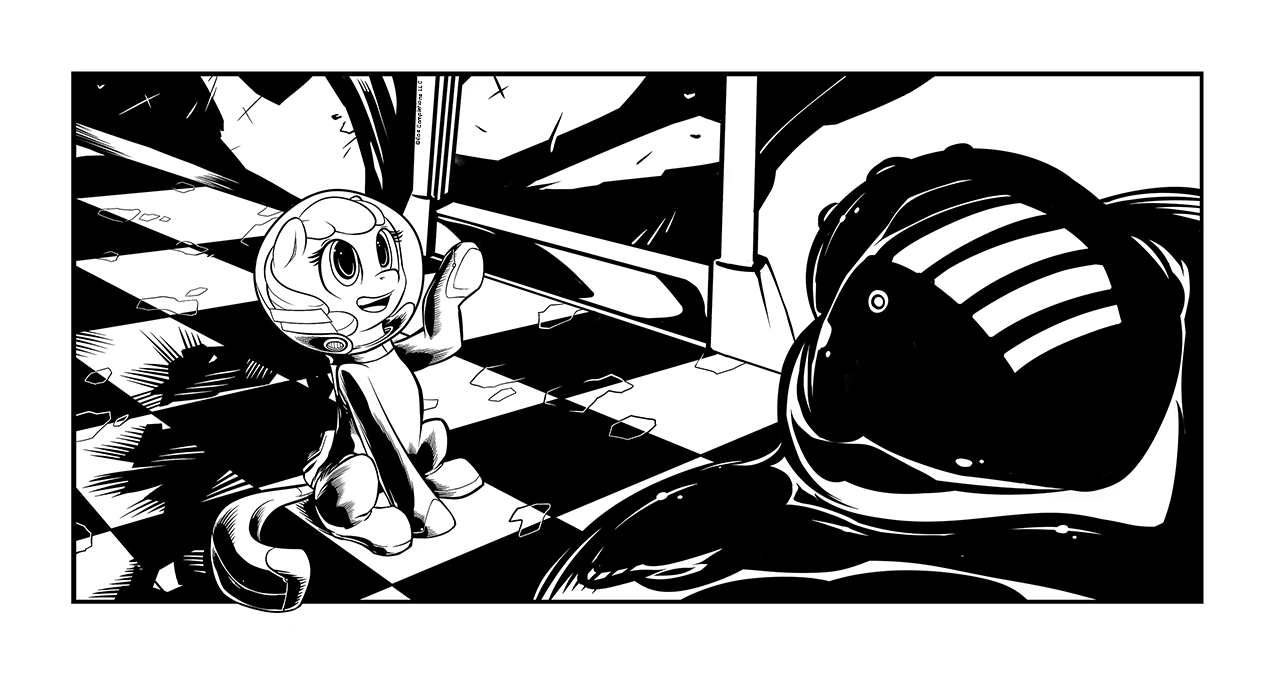
\includegraphics[width=0.9\linewidth]{image12.png}

\begin{intro}
我是独行于黑暗之路的雌马。\footnote{这句话是 Iron Maiden 的 \emph{Fear of the Dark} 歌曲中的一句歌词}

\begin{englishlyric}
    When I'm walking a dark road I am a mare who walks alone.
\end{englishlyric}
\end{intro}

\daytimeplace{11}{0:15 AM}{旭日避难厩,52号国道中段}{Solaris Stable, Big 52 SC Branch}

「滚出我的避!难!厩!」

旭日系统的电子合成声音在地下通道之中的无数个喇叭形成的超级立体声效果之下,如同阵阵雷声一般回荡。

帕比低头确认自己踩着的是一个白色格子,而不是和无底洞一样的黑色格子之后,蹲坐了下去。每一次她玩得开心得时候,老是有长辈突然跳出来扫她的兴。

「为啥啊?」

「因为你这个故障自律终端已经惹了够多麻烦了!」

帕比皱起眉头:「我不是驴子,也不是紫色的!不要叫我紫驴!」

「我是说你只是个机器马,而且低级到连个像样的字库都没装!你的愚蠢与无能让我的子网络重启了!」

帕比生气了,真的生气了!她站起来抬头怒视着面前的哨兵机器,用非常非常愤怒的目光瞪着他,不过她这个表情就像是把一个钢铁头盔扣到毛绒玩具头上一样,只会让这个玩具更……萌一些。

「喂喂喂!我不是机器,怕音和我这么说,赫瑞和提问者也这么说,所以这是一比……呃……几?」为啥说什么事情都会扯到数字?「反正是很多很多!」

「把错误加到一起不会得到正确的结果,018号设备,就算现在我的每个扫描仪都得到和之前一样的结果,你不过是个智能防护服而已,你里面装的那具小雌驹遗骨不能让你成为真正的小马!你不过是个塞满烂肉和骨头的疯狂机器!」

帕比举起蹄子指着哨兵,「别装聪明了蓝蓝!否则我要让你知道你是个……呃……那啥……超级书呆子!」

「我想这一点没什么好争论的,现在我命令你离开这里,018号设备,我就只想慢慢看着这些空空如也的走廊——直到永远。」

「但是我有事情要做,我才不走!」

旭日系统的声音顿了一下,然后又问:「你来这里搞什么?」

帕比皱了皱眉头,努力想了想……她来这里是干啥来着?为啥一件一件事情都要和这个傻蛋蓝音说?她想扮演无畏天马。「我要帮丑金先生找玻璃珠好让他告诉我妈妈在哪里……你能给我那些玻璃珠么,超超拜托?」

所以,你是来这里拾荒的?你把我在太阳城的一切努力都摧毁了还不够?你玷污了我的劳动成果现在又想来我家里抢劫?你够了!我唯一能给你的就是你立刻离开的最后通牒!」

「但是……我真的需要那些东西找我妈妈!如果你给我玻璃珠我可以拿别的东西和你换,就是个交易,和其他小马做的一样!」小雌驹低头在她的鞍包里面翻找着,想找点这个幽灵声音喜欢的东西。

「你没有妈妈,你是个机器,你简直是错上加错的典型,就像你的逻辑电路一个德行!」

这……不但很难听,而且是扯谎!妈妈绝对在哪里等她!帕比听到了录音也看到了妈妈的画!妈妈给她留下了很多留言。蓝音是个大坏蛋,帕比不想再听他说话了。

「音乐!」

帕比头盔里面的收音机开始播放声音盖过旭日系统的声音。

「而且就算你把某个雌性小马当做『母亲』的替代品,你的软件也已经是200年前的了,现在你的『妈妈』早已经化为枯骨了!」

「大声点!」

现在就算在头盔外面,也可以清楚地听得到DJ孤狼在说放射性和腐质的危险。

「好吧,既然你不听我的话,那你最好夹着你的『小马』尾巴赶紧滚蛋!」

「再大声!」音乐的音量让那个计算机的声音听起来就像模糊不清的背景。

「你不走是吧?」

小雌驹没有回答,蹲坐在地板上,无线电的声音吵到就连几米之外都能听得到。

「{\rt ……这就是为什么你总是要带上纯净水和一些辐特宁以及辐射药的原因。好了,就说这么多,接下来是L.P.的音乐时间,很多听众朋友说我的音乐都太娘娘腔了,有些坏DJ可能会说『我的电台我做主!』,不过我可不是那种DJ,既然你们要了,那就尝尝这个,十一分钟的《终末之马》!让你们知道指指点点我电台的后果……}」

「那我别无选择只好使用致命武力了。」

卫兵的面罩又一次变成了红色,然后立刻开始对帕比射击,大口径机枪的弹雨立刻在小幼驹胸口上开了好几个洞,粉色的粘液飞溅得满墙都是。

\begin{music}
结束了,我美丽的朋友。

\begin{englishlyric}
    This is the end, Beautiful friend.
\end{englishlyric}
\end{music}

帕比挣扎着站起来,但是她的前腿被削子弹掉了一大块,让她摇摇晃晃地站不稳。

\begin{music}
结束了,我唯一的朋友。

\begin{englishlyric}
    This is the end, My only friend, the end.
\end{englishlyric}
\end{music}

小雌驹艰难地依靠着墙,用唯一完好的前蹄站着,但是第二波弹雨打碎了她的玻璃头盔,虽然第一发子弹在头盔上弹开了,但是还是留下了蜘蛛网一样的裂纹,然后下一发子弹就把整个头盔打成了一堆闪亮的碎片,帕比眼睛的位置也出现一个大洞,顺带还丢了一只耳朵,甚至可以透过洞看到她的后背。

\begin{music}
我们精心策划的已经结束。

\begin{englishlyric}
    Of our elaborate plans, The end.
\end{englishlyric}
\end{music}

「我懂了,既然你有这么强大的再生能力,那么我需要改变战术,瞄准你的晶片。」「命运之石」漂浮在了帕比面前,不过那个哨兵瞄准帕比的身体,射出精确的三发子弹,就在可爱标记的位置。幼驹静止了一秒钟,就好像定格在了拿出武器的那个姿势,但是马上她就又动了起来,用自己的蹄子抓住了石头。

\begin{music}
我们存在的凭依已经消逝。

\begin{englishlyric}
    Of everything that stands, The end.
\end{englishlyric}
\end{music}

「妈妈不喜欢我弄坏其他孩子的玩具,蓝音先生,但是如果你总是用它们欺负我,那我就要打坏你的玩具,就算那会让我觉得难过!」帕比用剩下的一只眼睛低头看着地板,「你看,你让我踩到黑地板了,我玩输了,你这个傻蛋坏机器!」

\begin{music}
没有安宁或者惊喜,这就是结局。
    
\begin{englishlyric}
    No safety, no surprise, The end
\end{englishlyric}
\end{music}

「你的确很厉害,我从来没见过这么固执的终端,那么和你的动力源说拜拜吧。」另一次精确的点射打在小雌驹鞍包和身体之间,无线电咯吱响了一声听起来是停止了,但是马上又以小一些的音量继续播放起来。「这简直不可能,你已经没有处理单元和动力单元了,你应该停止活动了,请不要违反物理定律继续捣蛋了好么!」


\begin{music}
    我再也不能凝视你的双眸。
    
    
\begin{englishlyric}
    I'll never look into your eyes Again.
\end{englishlyric}
\end{music}

帕比用蹄子扶着墙壁,慢慢走向哨兵,她不可阻挡的势头被她身上的几处重伤而拖慢,飞溅在墙上的粉色粘液正在慢慢流回幼驹的身体。她脸上失去的部分开始逐渐成型,这重生并不会先长出骨骼后长出肌肉,而好像有谁在用蜡笔慢慢画出轮廓一样,先是线条然后出现色彩。「别闹了好吧,我又没做什么错事,为什么要欺负我,我真的只想交朋友,不管你是个虫子还是烂泥巴。」

\begin{music}
    你能想象之后的光景么,无穷无尽无拘无束!
    

\begin{englishlyric}
    Can you picture what will be, So limitless and free?
\end{englishlyric}
\end{music}

「你到底是什么东西?」走廊充满了绿色的光,让一切都染上了绿色,「哦,我明白了,我使用了错误的兵器。」卫兵在帕比身上的最后破洞补好之前撤离了走廊。


\begin{music}
    在这绝望的大地上,多么渴望一个陌生的新朋友。
    

\begin{englishlyric}
    Desperately in need\dots
    
    Of some\dots different friend, In a\dots desperate land?
\end{englishlyric}
\end{music}

为什么坏机器跑掉了?帕比现在该去找玻璃珠了,不过她需要谁给她指路,小雌驹连忙飞奔起来追着卫兵,「等等,很抱歉我不应该叫你虫子!别丢下我!我不想孤零零的,我要找珠子!」帕比走进了一个悬挂着各种走道的大厅,每一个座位上都坐着一个死掉的小马,还有一大堆骷髅堆在通向出口的大门边。「我会给你我所有的漂漂玩具,拜托了!」


\begin{music}
    迷失在无尽的痛苦之中
    

\begin{englishlyric}
    Lost in a Wilderness of pain.
\end{englishlyric}
\end{music}

在大厅的另一边,一个更大的哨兵出现了,它只带着一件武器——一个闪烁着蓝色火花的巨大铁管。「或许来点魔法能搞定你!」然后大炮喷出一道湛蓝的光束完全把帕比淹没了。


\begin{music}
    所有的孩子都已经疯狂。
    

\begin{englishlyric}
    And all the children Are insane.
\end{englishlyric}
\end{music}

小雌驹呆呆地站在那里,大大的眼睛之中的粉色光芒消失了,她张开嘴想说什么,但是她只是无助地倒在地板上。


\begin{music}
    所有的孩子都已经疯狂。
    

\begin{englishlyric}
    All the children Are insane.
\end{englishlyric}
\end{music}

一切都变成了黑色,世界变得如此遥远,妈妈……丑尸鬼……还有什么来着?帕比想不起来了,世界变得如此寒冷,她现在只想……躺下来休息一下,她好想睡觉……她是谁来着?


\begin{music}
    等待着那夏日的暴雨……
    

\begin{englishlyric}
    Waiting for the summer rain.
\end{englishlyric}
\end{music}

音乐声终于慢慢消失,无法听到歌声,在HUD上的所有光芒也慢慢消失了。

\horizonline

\unknowndaytimeplace

\pypr{「帕比啊,这就是你旅程的尽头吗?你就想这样结束吗?」}

小雌驹蜷缩成一个团,她不想听,也不想说,她只想这样呆在黑暗中,她终于可以不用去想妈妈还有多远了,她还要走多久才能找到另一个妈妈早已经离开很久的地方。

而且,蓝音太强了,他的坏机器把她打得都站不起来,为什么还要站起来再被打呢?一点意义都没有,她最好还是躺下来,至少这样没有那么难受。

\pypr{「我不觉得你真的想在这里就结束,你什么都没得到,你妈妈依然没找到,让蓝音这个出老千的赢了。为什么你要让他这个大骗子赢?」}

并不是帕比让蓝音赢,而是她不想再玩下去了,帕比知道坏蛋永远不会胜利,妈妈和她说过很多次,小马应该友好而善良,不要做坏事,邪恶的坏蛋绝对不会笑到最后,因为这不是小马做事的办法,你应该学会爱与宽容。

\pypr{「所以,你只是用你的爱与宽容让他做各种坏事?我明白了,但是……如果其他小马,不是你,让他知道坏蛋不会赢,怎么说呢,就是给他个教训之类的?」}

帕比不知道……她觉得蓝音应该学学什么叫友谊,或许谁可以告诉他这个样子交不到朋友。或许它会变成好马,或许这样帕比就可以和他做个交易让他交出玻璃珠然后就可以找妈妈去了,这样就太棒了。但是……谁能打得过那么厉害的坏机器?帕比不知道谁能有那么厉害……{}

\pypr{「或许你就可以,小家伙……睁开眼睛,然后剩下的交给我。」}

\horizonline

\daytimeplace{11}{0:30 AM}{旭日避难厩,52号国道中段}{Solaris Stable, Big 52 SC Branch}

帕比的眼睛再一次睁开了,并且闪烁着蓝黑色的火焰,幼驹慢慢地站了起来。

「猜猜是谁回来了,大坏蛋?」小雌驹的声音变得不一样了,就好像是从很遥远的地方传来,并且带着回音。

「我一定是计算错误了,一发炮弹显然不够,那么,请再吃一发。」这个装备水晶炮的哨兵再一次把闪着蓝光的炮口瞄准帕比。

小雌驹一副不屑的表情挥了挥蹄子,「免了,老娘减肥呢。」天花板上的一个钢梁被暗色的光芒包围着飞了下来,像一个巨大箭矢一样把那个哨兵直接射穿。

\thpr{哇哦!酷毙了!你怎么做到的?教我好么?教我,教我!}

旭日系统的声音又一次在大厅里面回响着:「你觉得那点雕虫小技就能对付得了我?好好想想,我可是有整整一个机械师在下面等你!」

黑化帕比不屑地嗤之以鼻,「好啊,在下面撅起屁股等着,老娘这就下去把它们打开花!」

「{\mt 红色警报!红色警报!启动安全系统,锁闭所有防爆门,这不是演习!重复一次,红色警报,红色警报,从1到12号仓库全部警戒!}」

一个了无生气的电子合成音在走廊里面响了起来,随之一打哨戒机枪从天花板弹出来,朝小雌驹扫射。

「滚边儿去!」幼驹毫不在意地走过破碎的哨兵机器,天花板上的机枪喷着火舌倾斜着如雨一般的金属风暴把黑化帕比打得满身都是洞,粉色的云雾包围着小雌驹,在这团雾气的中间有一道蓝色的剪影,正是这剪影给予了帕比形体和力量。一道巨大的铁门在她面前落下,挡住了她的前进步伐。

「哦?禁止进入?哈,坏孩子最喜欢打破禁令!」

粉色的云雾撞向大门,起初看起来没发生什么,然后随着一阵金属撕扯的悲鸣,大门在如雨的电火花之中被抬了起来,蓝色的线扯着大门,直接把大门推了上去。

\thpr{超超超超超炫酷!让他知道什么叫嗷嗷厉害!干得好,耶!}

就在大门背后,三个装备着能量炮的哨兵机器已经等在那里。「将军!」旭日系统的声音被大炮的轰鸣声淹没。

不过光线完全打在了又一次放下的大门上。黑色的雾气穿过门缝随着走廊地板蔓延,将那些机器哨兵漂浮起来,他们发出一阵滋滋声然后爆成了蓝色的火花,接着大门又一次打开了。

「你不过是个魔法畸形!为什么你不放弃然后消失?你这样的错误必须纠正!」

黑化帕比冷笑着:「由谁纠正?你这个残杀幼驹的自大狂?我想该被纠正的是你!」

\thpr{说他才是笨蛋,他才是虫子!}

「拜托帕比,我正忙着呢!」黑化帕比一脸不耐烦地说:「你有你的说法,我有我的,对吧,这叫『私家领域』!」

\thpr{喔,好吧,抱歉,那我乖乖坐着看,好吗?}

「乖孩子,呃,我们刚刚说到哪里了?哦,对了,去踢某个闪闪发亮的金属屁股,出发!」邪恶的幼儿园怪物哼着小调轻松打破一排防爆门继续前进。

「{\mt 入侵警告,动力区被入侵,启动防御系统!}」

旭日系统的声音代替了无腔调的系统音:「畸形,你的确很厉害,不过你还没有见识到旭日科技的真正力量!」

黑化帕比皱了皱眉头,「我说,你有听那丫头的话么,『我是一只小马』!」然后她冷笑一声:「好吧,这台词应该留给小家伙说……哦哦,好大一机器马!老娘好怕怕哦!」

「没错,你知道什么叫电磁炮么?」

一台比主战坦克还大的巨大双足战斗机甲立在仓库之中,它上面安装了无数武器,不过最瞩目的还是它左边的巨型大炮。

「这可是普罗米修斯计划用的同样武器。」

梦魇幼驹打了一个哈欠,「你真的有在用功么?我说,我虽然可以在这里站一整天等你召集你的不管什么狐朋狗友然后组织个像样的大决战,不过抱歉,今天我赶时间。」幼驹毫不在意地继续前进,随意挥了挥蹄子,那个机甲就大头朝下砸在了墙上。

\thpr{哇哦,哇哦!你可以教我这一招么?我现在只能让石头飘来飘去!}

另外一群炮塔继续给黑化帕比沐浴着弹雨,但是那些子弹一点点阻碍都没有,只是让围绕着幼驹的粉雾更加浓厚了。忽然小雌驹停了下来,嘴角露出一个邪恶的微笑,「你不觉得少了点什么吗?我是说,至少应该有点经典镜头才对。」

浓密的粉雾在帕比身后形成两道夜空色的黑影,开始看起来只是淡淡的剪影,但是很快就变成了一对蝙蝠一样的翅膀。

\thpr{呃,这是翅膀么?我们要飞么?我们不会要飞吧……{}}

黑化帕比哼了一声:「那还用说,不然你觉得翅膀是干啥的?」

保护主机室的防爆门冒出一阵电火花,然后和它的兄弟一样被打开了,这个房间看起来像个大大的圆井,中间是一个巨大机器,被一堆形状奇怪的设备围绕着,只有一个梯子从墙边落下来。

\thpr{别,别别别别……等等……不要……我不要飞!好可怕啊!呃……我是说,一点都不酷,真的一点都不酷啊啊啊啊!}

帕比眨了眨飘散着蓝色烟影的双眸,然后用蹄子按着头盔正面,「我说,老娘干活的时候能安静点么,等搞定这家伙我们再接着聊?」

% NOTE: 修正省略号过多

\thpr{呃……好——吧……不要翅膀……好么?}

黑化帕比泄气地举起蹄子,「好好好,听你的,不要翅膀!」翅膀随之消失了,「这下行了吧?」

\thpr{对对对!非常感谢怕音小姐!我不是那么害怕翅膀,你知道的……只是……呃……我对于用它们来那啥有点……啊……无所谓啦……就这样。}

「随你便啊!先让我们送蓝先生回老家。」小马看了看楼梯,然后叹了口气爬了下去,前面还有五个要爬。

「等等!」旭日系统的声音从喇叭里面传出来,「我觉得现在是不是应该讨论一下停火协议?」

「现在说这个是不是有点晚了,大家伙……这是给你一个教训,让你看看敢招惹超自然力量的下场。」黑化帕比顿了顿,然后说:「不,我想你学不到什么,我应该彻底把你删除才对。」

「我早应该预见到这一结果,我输了!」

「没错,真糟糕,你烂透了。」

\thpr{耶!他认输了,哈哈,现在我们来跳舞庆祝胜利吧,就像帕比舞那样,你要唱『啊哈哈哈哈哈,谁最厉害,我最厉害!』一边跳一边唱哦!}

「没错,不过等我结果它之后再跳。」黑化帕比一边说着一边爬下第三层。

\thpr{哎?你不是已经赢了么……}

「哈,差不多,不过有时候光是赢了没用,要保证你的对手之后再也不会来烦你才行,相信我。」

\thpr{喂喂喂!等等,我们不应该欺负已经说对不起的小马!}

黑化帕比站在走道上叹着气:「但是你在太阳城已经这么做了!他说抱歉然后你还引爆了那个弹头!」

\thpr{那不一样!那个东西只摧毁坏蛋机器,蓝先生不是坏蛋机器你这个小傻瓜,它只是个唠叨机器而已!}

「拜托,别告诉我你真的要这么做……好吧,你真的打算放过他?那好,小家伙,至少我们确保他不会再用魔法炮轰我们。

\thpr{但是他已经认错了!他说不会再犯了!}

「对啊,不过你觉得它有诚意么?而且不管怎么说它只是个机器,又不是有小马会受伤。」

\thpr{声音先生和声音小姐都是机器,提问者也是,他们都是我的朋友!声音们不是……不是可以让小马玩弄的玩具!如果你对他们好他们也会对你好的!除非,你不想和他做朋友。}

「为啥我们要和这个控制欲爆棚的自大自律智能做朋友?」

\thpr{好吧,又开始说不明觉厉的奇怪话了,如果你不想和他做朋友,我想!该我了!}

「随你便,就好像你能……」帕比的双眸再一次变成了粉色,她眨着眼寻找着某个显示器或者什么的看起来像蓝音先生的脸一样的东西,「哦,嗨!很抱歉刚才是我的朋友,她有那么一点……呃……不开心……」

这有点,奇怪。帕比不太清楚她的感觉,或者说她怎么让怕音做出刚才的表演。不过如果用她的话来说,就好像是你把玩具借给其他小马玩一样,你懂的,并不是说你不相信他,只是害怕他弄坏玩具然后妈妈就不开心了,而且帕比也没有那么多太空服,所以就简单的问他要回来了啦!毕竟那是帕比的太空服。不过帕比完全不知道,曾经打破梦魇的侵占是需要非常大的魔法彩虹才能做到。

「如果你和自己吵完了,你能和我解释一下到底发生了什么吗?」旭日系统的声音打断了帕比的思绪。

「呃……好啊!你想知道什么蓝音?」小雌驹笑着坐在地板上,反正她也不知道应该对着那里说话。

「你能从刚才发生的事情说起么?」

「好啊,怕音帮我告诉你那样作弊胜利不对,然后你说抱歉认输了。于是我让她跳个胜利舞蹈但是她不想跳舞想要欺负你所以我不让她玩了对了我差点忘了!」帕比站起来对着旭日系统唱道:「\textbf{啦啦啦,谁最厉害,我最厉害!}」然后转过身来,吐出舌头做了一个鬼脸,「耶!」

「好吧,真有趣,真的……很抱歉我笑不出来,」旭日系统顿了一下,「那么然后呢,你要走了么?」

帕比轻轻敲着自己的头盔想了想,「啊……我记得我要做什么来着?声音先生!我们下来干啥来着?」

「{\mt 读取主要任务列表:滚动的回忆,任务目标,从旭日避难厩的研究中心得到六个记忆水晶。}」

帕比一副睿智的表情点了点头,「哦哦,对了,玻璃珠!啊,小蓝!我们现在是朋友了,可以给我玻璃珠了么?超超拜托?」

「谁和你是朋友!你不过是个入侵者!我必须将你消灭!不过既然你看起来蹄高一招,我可以和你交涉,如果你帮我做点小事,你就可以随意进入研究区域想拿什么就拿什么。」

帕比皱了皱眉头,小事,多可怕的词。「呃……我不太清楚,我要去准备餐桌还是去倒垃圾呢?」

「绝对不是!你怎么会想到那里去?你要去这个避难厩已经遗弃的区域,然后启动通信中心,等你做完之后,回来这里我带你去研究区域。」

黄色的小雌驹开心地点点头,「耶,我喜欢按按钮!超简单!」

「那好,就这么定了,仔细听好……」

\horizonline

\unknowndaytimeplace

怕音安静地盘踞在帕比意识的角落之中。她非常清楚她失败在哪里,她太过急躁,在两百年的等待之后,急躁毁掉了她的胜利,这个幼驹正在失去她的信念,让她自己滑向深渊,所以她在这里汲取幼驹绝望的力量。但是在刚才急躁的冒进之下,她再一次给了幼驹希望,而幼驹的意志又足够强大以打破她的魔咒。

但是梦魇并不会在一次失败之后就退缩,在如此甜美的猎物已经送到嘴边的情况下更不会轻易言败。小雌驹还有希望,就像一盏明灯在黑暗之中给她指明方向,给她前进的动力,但是在那个希望失去的那一天会发生什么?你爬得越高,摔得越重。小马的旅途已经接近尾声,而声音要做的,就是在这条大路的尽头静静等候着她的到来。

\horizonline

\daytimeplace{11}{3:00 AM}{旭日避难厩,52号国道中段}{Solaris Stable, Big 52 SC Branch}

「{\mt 警告。发现敌对生物,总数:18,威胁等级:非常致命,建议立刻撤退。}」

三个肉食灵挤在屋子的角落里面,惊恐万状地想要把同类推到外面去,帕比已经放弃抓一个最大的做宠物了,因为它们实在太快了,所以她现在想要抓一个小的。不过就算是小的也跑得很快,就算掉腿掉翅膀也不让帕比抓住他们。

「唉,这些小可爱都怎么啦?宠物应该毛毛软软的一个团,而不是到处乱跑,像个……疯狗一样!」

几个骷髅和无数机器残骸躺在通讯站的地板上,就和其它旭日建筑一样,为了得到更好的信号强度,这个房间在基地最高处,有一扇大大的窗户可以眺望见铁锈庄园,不过经过多年风吹雨打,一个强化玻璃破掉了,现在整个房间就是肉食灵的巢穴。

肉食灵是贪吃灵在辐射之下变异而成的巨大掠食生物,它们的身体比它们的祖先大很多,并且进化出有剧毒的尖锐牙齿,不过它们巨大的翅膀让帕比觉得它们是大公主级别的可爱毛球。小雌驹完全忘记了她的任务,在这些小马国最可怕的掠食动物的巢穴之中追逐了它们一个多小时,不过完全没什么结果,这些有灵性的生物一见到帕比就纷纷飞走决不让她靠近。

帕比不开心地叹了口气:「我只是想和你们玩玩儿而已!」她沮丧地哼了一声,然后走到了控制台面前,想要找到让这个屋子再一次工作起来的按钮,就像蓝音先生说的那样,「呃……红色按钮,红色按钮……为啥他们总把重要的东西藏起来?喂,声音先生,那破按钮在哪二?」

「{\mt 扫描中,发现启动开关,将物件标示在罗盘上。}」

帕比走到墙面边的按钮上,在用力敲了几次之后,房间的灯亮了,几面屏幕上也出现了蓝色的字,帕比皱了皱眉头,她更喜欢粉色的,不过既然这里是蓝蓝的家,所以蓝色的字也可以。

「好吧,搞定,让我们……哦天哪我简直不敢相信!」帕比瞪大了眼睛看着躺在地板上一动不动的一个小肉食灵。

「一个不跑的漂漂小蝴蝶!」幼驹开心地跑过去紧紧抱起那个小东西。「我会养你我会抱你我会永远爱你!」

「{\mt 分析中,死亡肉食灵尸体,威胁等级:无。}」

「你的名字就叫毛球!你喜欢么!」帕比把死去的生物丢到空中,然后在它落下的时候接住。「哦哦,你很高兴!谁最爱你,我最爱你!」

「{\mt 建议:捡起死去生物不健康。}」

帕比把那个生物放进背包里面,然后挥了挥蹄子,「别嫉妒声音先生,我也喜欢你!对毛球好一点。」

「{\mt 警告,该程序并没有嫉妒,死去的动物可能会携带疾病。}」

「好吧,你没嫉妒……真是的。」幼驹压低声音说:「傲娇……」

旭日系统打断了防护服的回答,用房间内的喇叭大声说:「非常好D018,你干得很棒,我会把去研究区域的最短路径发送给你然后取消警报,你想去哪儿去哪儿,不过很抱歉我先失陪了,既然通信站上线了,那么我还有一个大陆去征服!祝你过得愉快,在玩儿完之后赶紧离开避难厩。」

\horizonline

\daytimeplace{11}{4:30 AM}{旭日避难厩,52号国道中段}{Solaris Stable, Big 52 SC Branch}

当帕比从洞口出来的时候,融金正坐在篝火前吹着口琴。他立刻注意到幼驹,抬起头问道:「你去了好一会儿,找到水晶球了没有?」

帕比笑着更正到,「是玻璃珠!」一打记忆水晶飘了出来,「它们够吗?现在你可以告诉我妈妈在哪里了么?拜托,拜托!拜托了!」

老木乃伊尸鬼挥了挥蹄子,「等等,我检查一下这些……」他拿起一个水晶然后点了点头,之后小心地把其它记忆水晶都收起来,「很好,没错,就是这个,我想我可以……」尸鬼一下呆住了,「喂,你干嘛背着一个死肉食灵?」

黄色的幼驹转了转身让尸鬼仔细看她背后的尸体,「你喜欢它吗?她是毛球!我的宠物!我一直一直一直想要个宠物!我们可以一起玩,比如追蝴蝶,和小雄驹玩,或者做煎饼!」

融金摇了摇头,「但是……那东西已经死了!快丢掉!」

「为啥?毛球是我的宠物,我不能抛弃她!我找到妈妈之后她一定也会喜欢她,是不是很棒!」帕比微笑着想起了之前的交易。「好吧,我妈妈在哪?」

尸鬼笑了笑,「好吧,小幽灵,你既然做了你的事情,我来告诉你,几个月之前我在象牙塔见到了阴雨·黛丝女士,她正在那里召集幸存者。」

防护服发出叮的一声,通知帕比任务目标已经改变。

「{\mt 新目标:象牙塔,路径计算完毕,显示在罗盘上。}」

「耶!太空战士安德洛队长的新冒险!砰!噗!直飞月球!」小雌驹正准备跑开却被尸鬼扯住了尾巴。

「等等!象牙塔可不是幼驹去的地方!那里现在已经是铁骑卫\footnote{铁骑卫(Steel Ranger):陆马军队,拥有苹果杰克的部门(战时科技部)研发的动力装甲,火力强大,防御能力极高,但铁骑卫中也有一些学士不参与战斗}的前哨站了!那可是两百……」融金看着帕比的双眸,他可以看得见小雌驹眼中的希望和信念,认为一切都会快乐安好的强烈信念。\thpr{我怎么可以说得出口。但是如果她发现}——\thpr{不,那不是你的问题,融金,她问了,你回答了,交易完毕,让她走吧,别回头看了。}

% NOTE: 遵照英文原版改

「什么事,丑金先生?」帕比歪着头等他说完。

融金撇开了视线,低声嘟囔着:「只是……别惹他们生气,他们比较特别……祝你好运,小幽灵……」

「谢谢你木乃伊先生!我找到妈妈之后我会告诉她你对我很好!拜拜!」小雌驹开心地蹦走了。

「记得丢了那东西!太恶心了!」

「我听不懂你说什么!啦啦啦!」帕比消失在石头后面,留下老尸鬼和他的新财宝。

融金叹息着,看着这些记忆水晶,把它们仔细收好,「过去的事情就让它过去,别在意老木乃伊,别在意……」

\horizonline

\daytimeplace{11}{7:00 AM}{象牙塔北,52号国道中段}{North of Ivory Tower, Big 52 SC Branch}

{\rt 早上好听众朋友们,这里是孤狼的52电台!这里唯一的电台!我先感谢那些带着对讲机一直告诉我52号国道新闻的朋友们:我爱你们!没有你们的帮助我什么都做不到,大家听好了:如果不是你们一直告诉我新闻52电台就是个聋子,我也没办法警告那些在52大道上的旅者哪里有危险。在这个世界分崩离析之前这些小马就是52号国道的守护者,所以如果你们遇到他们,请和他们好好打招呼,毕竟他们关系到你们的货物是否能安全达到目的地。

好了,接下来是新闻事件,我们来听听这条大道上的新事件,看起来在太阳城之后,内战的火焰正在沿着52大道蔓延,我听到的最新消息指出,似乎铁骑卫因为意识形态问题而分裂成为两个派系,其中一部分认为他们应该继续保护上古科技,而另一部分认为他们应该用那些科技去帮助其他小马。

现在问题是,两个派系正在火热交战中,那些想用科技帮助小马的铁骑卫,似乎以他们古老的创始者为他们的派系命名——苹果杰克!但是现在象牙塔正在猛烈交战,所以你懂的,请避免经过象牙塔以及周边地区,如果你不想被一大群穿着动力装甲的小马抢劫或者卷入他们的圣战中,最好还是别从那里过,先在铁锈庄园或者花椰菜镇等待事态平息!

我听到盐块城的白先生正在组织一队佣兵清理太阳城的周边地区并且保护从盐块城到铁锈庄园的安全。看起来白苹果也打算在那个刚醒来的太阳城上分一杯羹。我只想提醒白先生一句话,记住那个把你屁股上的核弹拆掉的小幽灵,在太阳城里不只有歹徒,还有那些不想打仗的老弱病残,所以请你提醒你的手下,在扣板机之前先好好看看目标,好么?}

一阵阵爆炸声从远处升起浓烟的方向传来,帕比慢慢跟着罗盘上的红色箭头走上了52大道的柏油路面,将她的滑板车放在路上,开心地跳上去冲向下一个战火纷飞的地方。

\begin{music}
路途充满尘土,

\begin{englishlyric}
    The roads are the dustiest,
\end{englishlyric}

\medskip

阵阵狂风袭来。

\begin{englishlyric}
    The winds are the gustiest,
\end{englishlyric}

\medskip

大门锈迹斑斑,

\begin{englishlyric}
    The gates are the rustiest,
\end{englishlyric}

\medskip

食物坚硬入咽。

\begin{englishlyric}
    The pies are the crustiest,
\end{englishlyric}

\medskip

歌声仍然响亮,

\begin{englishlyric}
    The songs the lustiest,
\end{englishlyric}

\medskip

朋友忠实可靠,

\begin{englishlyric}
    The friends the trustiest,
\end{englishlyric}

\medskip

这就是回归家园之路!

\begin{englishlyric}
    Way back home!
\end{englishlyric}
\end{music}

\clearpage

~\vfill

\begin{note}
升级(Lv 11)

新专长解锁:石墙——你在战斗中不那么容易被击倒。

新任务专长解锁:移动梦魇(等级2)——你已经看见月亮之后的阴影,现在你可以将身边的毒雾塑造成你想要的形状。
\end{note}




\chapter{风暴}

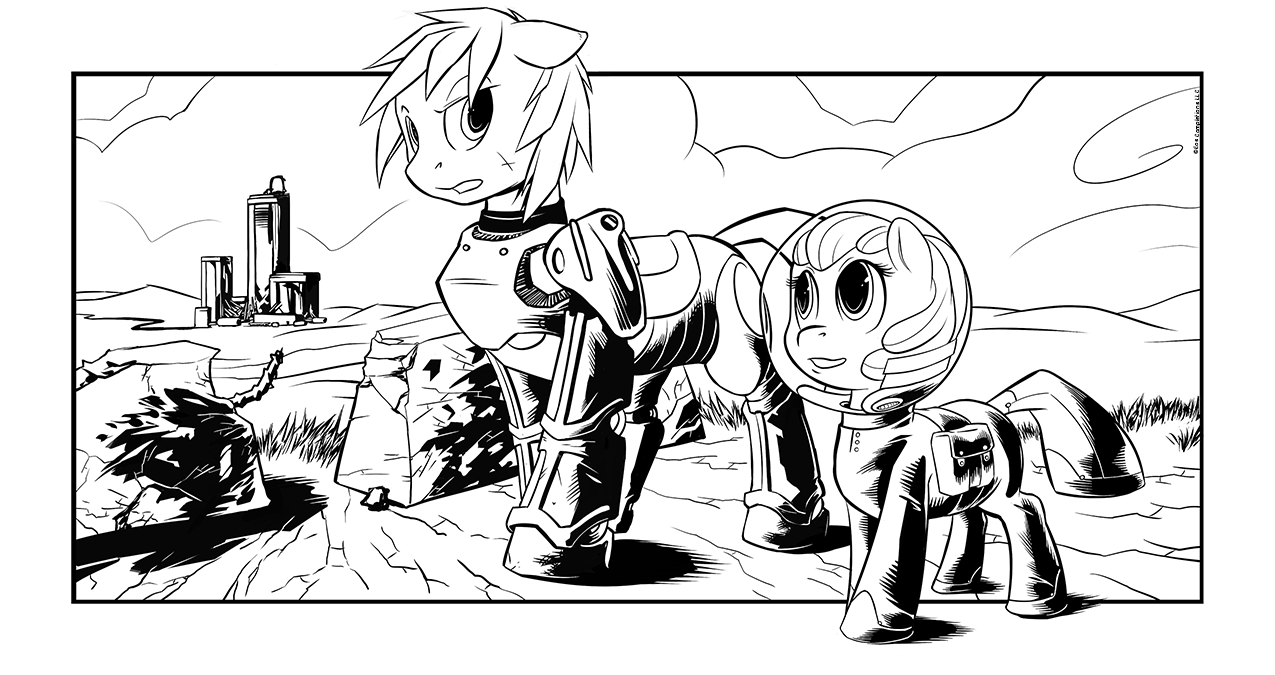
\includegraphics[width=0.9\linewidth]{image13.png}

\begin{intro}
我说,你见过下雨么?
\end{intro}

\daytimeplace{11}{18:00 PM}{象牙塔,52号国道中段}{Ivory Tower, Big 52 SC Branch}

象牙塔是个强化陶瓷外墙的巨大白色建筑。在战前这里曾经是个研究设施,和平部的员工在这里寻找神秘科学部\footnote{神秘科学部(Ministry of Arcane Science):大战时期由暮光闪闪成立的部门,负责魔法研究,\emph{FoE} 中的天角兽「女神」便是该部门的「产品」之一}和战时科技部\footnote{战时科技部(Ministry of Wartime Technologies):大战时期由苹果杰克成立的部门,主要通过陆马(物理)方式研发和制造科技产品并用于战争}研究成果的非军事用途。

现在象牙塔是铁骑卫在52号国道的唯一据点,主要因为这里是附近唯一没有被旭日公司碰过的高科技设施,而稍微有些理智的小马都不会碰旭日公司。

没错,旭日公司,那些疯子,他们将一个收音机和一个吸尘器组装在一起做成了第一个声波武器然后交给一个稀里糊涂的女仆。还发明了第一个带有窃贼监测消灭功能的门铃——这个门铃电死了六十多个上门服务小马和一整排的卖马芬小孩子。

整个建筑都被一道带有护城河的城墙围着,并且带有自动炮台和地雷阵。这个城墙经过一个世纪对抗从土匪到山贼的战斗之后。现在看起来相当糟糕。炮台早已经被摧毁,地雷阵也基本没有了,就连城墙也饱经创伤。在唯一还算完好的护城河之上有两座吊桥,一座在西边一坐在北边,在吊桥外面有各式各样的棚屋,大多都是一些旅行商队的仓库以及那些和铁骑卫做生意的小马过夜歇脚的地方。

不过现在北边的棚屋已经基本被拆光了,而各种垃圾被收集起来在桥北边堆出一个路障,同时西边的那些战前建筑也被垒上了沙包,并且飘扬着苹果杰克卫士的旗帜。

这个小小的要塞被一打小马守卫着,其中甚至还有一些穿着战斗鞍的年轻小马。一对武装到牙齿的铁骑卫穿着它们传统的动力装甲正守在桥头。另外一个则带着新兵在象牙塔周围的乱石滩巡逻。第四位则站在临时指挥所里面和一个年轻的佣兵争执着。

「你说的我能做到,但是我现在想先要一半定金,还有一些等离子武器。」赫瑞塔抱着双臂坐在椅子上,把自己的狮子腿翘在桌子上。

那个骑士一脸不爽地摇了摇头:「你当我是啥?卖房车的?我给你一柄动力长矛已经算你好运了,其它的东西只有你完成工作才给你。」

赫瑞塔轻蔑的哼着,「我是个枪手,你那花哨的肉搏兵器我用不上……给我三个离子手雷,现在给我两个,回头再给我一个,还有俩EMP地雷我就依你。」

「给你俩EMP手雷,事成之后再给你一个离子手雷和离子地雷,最终价。」小马用蹄子指着狮鹫说。

赫瑞塔耸了耸肩,抓住那只蹄子握了握,「成交,先付一半瓶盖。」

「然后你拿着钱飞走?我才不信你,而且你现在拿着钱又啥也做不了。」

狮鹫叹了口气:「你知道我怎么想的吗,我觉得你没有那么多瓶盖,你是想让我去捣乱,然后你们正面进攻,最后你们用基地里面的钱付给我……我不觉得你们四个铁骑卫和十五个新兵能够正面攻破一个至少一打半重装备小马防守的城堡。」

那个帕拉丁举起了蹄子,「好吧好吧,你这个守财奴,现在就给你一半瓶盖!别觉得我会因为这件事情感谢你。」

「谢意买不来子弹,我想这可以成交了,」狮鹫又耸了耸肩,「我马上就出发,希望你的手下别把事情搞砸了。」

「你干完活回来和书记梅隆说,如果你想参加正面进攻的话,我会再给你点别的,比如一些收集到的装备。」

赫瑞塔还没开口,但是她面前的小马举起一只蹄子示意她等等。

「冷浴收到,请报告。」小马压低声音,但是狮鹫竖起耳朵也能听得很清楚。

赫瑞塔坐在桌子面前打着哈切,不管怎么这事情和她无关,等到入夜他就出发,想想他们已经允许她从铁骑卫尸体上扒装备了,说明这些小马已经没什么选择了。

「再说一遍?你射杀他多少次了?」那个帕拉丁惊讶的叫起来:「高斯我觉得你不可能杀死一个东西两次以上……」

听到这句话赫瑞转头看着那个用对讲机说话的小马,不过现在冷浴完全没有注意那个佣兵。「你到底想要说什么,你确定那是敌军么?」帕拉丁停顿了一下听着对面的回答然后说:「所以,你只是因为觉得他有点诡异所以就开枪了?」

狮鹫听到这句话跳了起来:「肏你娘,告诉你的手下不准欺负帕比!」

\horizonline

\daytimeplace{11}{18:30 PM}{象牙塔,52号国道中段}{Ivory Tower, Big 52 SC Branch}

黄色的小雌驹,蹦蹦跳跳地来到小小的前线,看着那锈迹斑驳的路障,对上面的卫兵说:「嗨漂漂马!我叫快乐帕比,你看到我妈妈了么?」

内心和身上铠甲一样上锈的卫兵疲惫地看着帕比——他已经被连续几天无休止的战斗折磨得痛苦不堪,而且和他战斗的并不是强盗或者奴隶贩子,而是他曾经的挚友和老师。而这个小雌驹却一点都没在意对方的情绪。

帕比继续和护送她的卫兵讲着自己的故事:「……所以,即使镇长要赶走了机械战马,他还是决定去拯救城市。因为……你懂的,机械战马并不只是个机械,他也是超级厉害有正义感的小马!」小雌驹完全没有注意到那个卫兵不断上升的不耐烦情绪,「但是我刚看到那里妈妈就关了电视不让我看了,我不知道为啥她不允许我看那种电影,你说,机械战马绝对是个好马,所以最后她一定会赢,是吗是吗?」

帕拉丁高斯重重叹了口气:「对,你说的没错,不过我并不是你说的啥机械战马,我是阿杰铁卫!完全不是一回事!」

帕比咯咯笑起来,「你真有趣,机械战马阿杰铁卫!我喜欢这个名字!」

「好吧,……随你便,摆脱,至少把那个肉食灵尸体放起来,恶心死了!」小雌驹还背着那个死去的肉食灵,没有一位小马会对这个已经没有一只腿和一只翅膀的前肉食灵感觉到一丝的怜悯之情,不过小雌驹还是把它当宝贝一样带着。

帕比皱起眉头,「但是小毛球肯定也想看漂漂马,他会乖乖坐好的,我发誓!」

帕拉丁以蹄覆面,「尸体当然会乖乖坐好,但是……哎……恩……这附近有专吃宠物的怪物,所以可能会……」帕拉丁心中默默地对这个幼驹扯谎而自责。

「吃宠物?在哪儿?毛球很危险!」小孩子马上把那个小肉食灵塞进背包里面,睁大眼睛看着周围。「在包包里面躲好,我来收拾他们!」

高斯看着刚好撞上的仨随从笑得满地打滚,哑口无言。而帕比也一起笑起来,「什么事这么有趣?」

高斯避开他们的视线,拿出自己最正经的表情,「这才对,你要小心哦,吃宠物的怪物哪里都有!现在跟我去见长官吧。还有你们仨!别在那里傻笑了,赶紧给我看大门去!」帕拉丁走过那几个年轻随从,小黄驹屁颠屁颠地跟在后面。

「好的好的,阿杰铁卫机械战马!我们什么时候去打击罪犯?」

「我再说最后一次,我的名字叫高斯,帕拉丁高斯!」公马叹息着,「我绝对不会要孩子……」

这对活宝终于走到了指挥部,公马打开门让帕比先走了进来,这个建筑曾经是一个学校,不过现在大部分都已经坍塌,只剩下几个房间还勉强保持完好,在这个小小办公室的另一边坐在桌子后面的是另一个穿着铁甲的小马还有赫瑞塔。

「赫瑞!」帕比开心地一蹦三尺高,径直飞扑向狮鹫,而后者侧身闪开,然后抓住帕比的后颈将她拎了起来。帕比微微挣扎了一下,来回张望着寻找着她的朋友。「嘿,你跑哪去了?」

「我说了『再见』就是改天再见面的意思,你还在往南走么?」狮鹫一边说着一边把帕比放下,拍了拍她的头盔。「帕拉丁伙计,这个是我的老朋友,在我干活的时候能帮我看好她么?」

冷浴歪着头一脸疑惑地看着小雌驹,「这个……小马被射中四次但是看起来毫发无伤的样子,而且她看起来心情不错,我不太清楚我能不能照顾……高斯,叫诘责书记进来。」

帕比并不太关心那个帕拉丁,因为见到赫瑞实在太开心了,「没错哦,妈妈就在桥对面的那个白屋子里面!我路上看到好多漂漂马,还有阿杰铁卫机械战马!」小雌驹终于抱上了狮鹫,「我好高兴见到你,这一次你不会丢下我了吧!」

赫瑞塔清了清喉咙,避开幼驹的视线。「呃,实际上……我正要去做一些事情,不过如果你等我的话,我很快就回来。」

帕比皱了皱眉头,小心地问道:「呃……你会带上丝尾一起去么?」

「丝啥?哦,那个玩偶,当然,为啥不带他?」

小雌驹松了口气,「没什么,让它帮你吧,她很厉害!」

狮鹫拍着小孩子的头说:「很好,乖乖和铁骑卫呆着,别惹他们生气也别乱跑,我一会儿就回来带你玩,好么?」

「耶!」帕比挥着蹄子送走赫瑞,然后呆在房间里面好奇地看着其他马。

\horizonline

\daytimeplace{11}{19:00 PM}{象牙塔,52号国道中段}{Ivory Tower, Big 52 SC Branch}

诘责书记是一个常年负责训练随从的老马,他冷酷而又铁血的训练手段让每一个新兵都对他心有余悸。只有一种办法能让这个老书记看得起你,把每一个任务都完成得尽善尽美。而当他加入阿杰铁卫的时候,很多人都怀疑他的这个选择,甚至很多随从都觉得他是个间谍。

诘责一边看着帕比一边对冷浴说:「中心城尸鬼有和通常尸鬼一样的腐烂外表,我不觉得她像是其中之一。」

帕拉丁叹了口气坐在他办公桌背后,「那你觉得她是什么?她可是挨了四枪,一枪在头上,三枪心脏。」

「也能给我一个红披风么?」帕比抓着诘责的斗篷一脸惊讶地说:「我喜欢金色的东西,就像漂漂大公主的颜色那样!我长大以后我也要做一个公主!我想要这个披风,拜托!」

「这些是咒符,不是给你玩的。乖乖坐好……」诘责回头继续说。「或许是某种死灵巫术,我可以确定……如果我能去图书馆的话我可以做一些研究,不过现在我只能推测……」

「为什么我不能玩儿?我可以给你东西换斗篷!这叫做交易!超酷的!大家都这么做!不像那次我用早餐换了两块大理石然后饿得发慌被妈妈骂……这次没问题的!」

帕拉丁无视帕比,点了点头说。「那么你的推测是什么?」

诘责看了看那个幼驹然后回答:「我不想拿我的斗篷和你换什么,乖乖坐那儿让成年马说话好么?」书记官叹了口气然后继续和冷浴之前的谈话,「我记得读过这些防辐射服的故事,它们显然没什么作用,在中心城的核爆之后几乎每个穿着它的小孩子都变成尸鬼了。」诘责停下来低头看着那个不停地扯着他斗篷的小雌驹,「不过这一个,我要说……或许我给他的防护服做一次检查就知道结果了。」

老书记把他的哔哔小马接上帕比衣服的数据接口,另一个蹄子按着幼驹让她别动,「安静几分钟好么?」

「我能抱抱你么?你好有趣,我喜欢你!」帕比想了想又说。「我也喜欢你的披风,刚才我说过了么?」

冷浴忍不住笑了出来,书记官瞪了她一眼,「好吧,你想怎么抱我就怎么抱我,恩……我们看看结果……」

诘责皱起了眉头,「从数据上看她已经死了,没有心跳,没有体温,甚至都没有身体,只是……两千多个骨头碎片和一百八十克有机物,完全不是尸妖。」

「呦呵,红斗篷也会说不明觉厉的话!」

「没错,诘责,别说那些不明觉厉的话,给我一个士兵听得懂的说法,我只懂轻武器和战车。」冷浴并不是不高兴,只是想提醒一下老书记官他现在并不是在讲课。

「我也不清楚,只能说她不是尸鬼。」诘责低头看着哔哔小马上的分析结果,「这个防护服的自律智能完全没有受损,所以我可以肯定这不是一个疯狂机器……哦,这一条很有趣,主医疗芯片在两百年前就故障了,这可是千分之一的故障率,或许是因为在启动中受到了电流冲击或者短路,所以只有备用护符在起作用。

「这一条哪里有趣了?」冷浴不解。

书记冷笑一声,「因为备用医疗护符和主医疗护符有很大不同。」

帕拉丁打了一个响鼻,「请一次说完好么,我可没时间做课后复习了。」

书记叹了口气,忽略帕拉丁的态度,「这个护符并没有内置医疗法术,只是有一个自动注射医疗药水的功能……等等,这个魔法回路上还刻着其它东西,是……斑马的咒文?医疗护符上刻着斑马咒文有什么用?」

这个咒文的结果现在就站在他们鼻子下面,用力扯着诘责的斗篷,「好吧,那咒语,保存了……一百八十克有机物?」

书记官继续看着他的哔哔小马,「对,这是一个有点腐烂的心脏,我要说……这个非常有趣,扫描表示有很多破碎的子弹漂浮在心脏附近,就好像它们没有命中心脏一样,我们看看护符的日志,或许能理解它的工作原理。」

他们俩聊天的内容太无聊了,帕比虽然是一个很有耐心的孩子,但是全小马国的耐心都没有那些哇啦哇啦哇啦麻烦,所以那个黄色的小雌驹开始把自己的蹄子伸进书记官口袋里面翻起来。她找到……一支笔,几张纸,一本书,一副眼镜……咔嚓……好吧,现在是一个单片眼镜,还有另一个单片……「咦,这是什么?」

帕比从诘责口袋里面掏出一个梳毛塑料玩具,那是一个白绿色鬃毛的独角兽,脸上带着一个大大的微笑,还有一个竖琴的可爱标记。

「哦哦哦,好可爱!」小雌驹抚摸着玩偶的鬃毛,「梳啊梳,梳啊梳……」

「怎么……喂,还给我!」书记官生气地把那玩偶从帕比蹄子上抢下来,然后塞回自己的口袋去。「玩你自己的玩偶好么,这个可动手办很容易就会弄……」诘责的视线对上了冷浴的目光,然后他才意识到发生了什么,「不不不不不不……咳……这个……玩具……恩恩……是我没收别的新兵的,不是我的别玩坏了!」

帕比一下子兴奋地睁大了眼睛,「不是你的?能给我吗?我会好好爱护她,给她梳毛,一起和她玩,我们会成为最好的朋友,就给她起名字叫糖糖\footnote{糖糖和天琴,同人中默认的一对CP}然后给她染个粉毛。」

诘责听到要给玩偶染毛的话之后立刻炸毛了,「她的名字是『天琴』,而且我不能给你,因为那是我……呃……我的一个学生的,应该仔细分类保管好!」

一个贱贱坏笑出现在帕拉丁的嘴边。

「别对一个玩具那么认真嘛诘责书记,我觉得让这个小雌驹玩一个小女孩的玩具没什么问题。」

冷浴一脸黄鼠狼给鸡拜年的坏笑。

「看吧,看吧,机械战马也说我可以玩,给我嘛,给我嘛!给我嘛!!」幼驹踮着脚去探诘责的口袋,但是这一次老书记官连忙捂住了自己的口袋。

「这个是我的总行了吧!天琴是我的!我不能给你因为我喜欢天琴!你满意了吗!嗯?」按下内心自爆按钮的书记官涨红了脸看着冷浴,「你可以从这个大姐姐房间里面挑一个玩偶,我想她会让你看她的卧室的,我想她没什么好藏的东西,对不对啊,机械战警?」

冷浴咳嗽了一下收起了笑容,「好吧,我带你去找几个漂亮玩具,小家伙,不过先乖乖让书记官做完他的工作。」

在新玩具的保证下,帕比一脸开心的表情乖乖坐在那里让红斗篷小马继续摆弄她的防护服。

诘责叹了口气,看了帕拉丁一眼说:「你能不要露出那副阴阳怪气的笑容好么,我干正事呢……」书记官叹着气。

「我的天……没开玩笑吧,他们居然在医疗护符里面放这种东西?」

冷浴一脸迷茫地看着诘责。「你发现什么了?你的脸色看起来不太好。」

「非常糟糕的事情……和平部的某小马为了不让这些小孩子死而做了非常可怕的事情……她不允许他们死掉。」

「什么叫不允许?」帕拉丁抬起一根眉毛问。

「我是说,这个备份护符的最后咒语是某种死灵术,虽然不清楚具体是什么不过看起来它的功能是把患者的生命灵魂束缚在它的遗骸上。」老书记官叹了口气,「不过,这个并不是太强的法术,我想花点时间研究一下就能解除它。不过这又回到了我们之前的问题上了——我需要图书馆。」

冷浴喃喃自语着:「就算是从爱的角度出发,怎么会有马做出这种……禁止你去死的东西,这个有可能么?」

「既然结果已经站在我们面前,我觉得可能,我不是死灵术专家,但是我可以说这个护符状态并不是很好,它在两百年的时间内都只靠一点点能量维持运转……我不知道怎么解释,这个法术逻辑上根本行不通!一定还有其它拼图碎片没有找到……或许……」

帕拉丁歪着头问:「所以说,基本上这个小鬼是某种幽灵?」

诘责摸着下巴,「我不太清楚,我还是需要再研究一下,不管怎么说我觉得这个护符是关键,没有它这只不过是一件破防辐射服,一堆粉色粘液和一个小雌驹的遗骨……你如果说这就是幽灵的话,我不这么认为,技术上讲这个可怜的小家伙根本不可能站起来,但是现在她却和一个孩子一样活蹦乱跳,不管记忆上还是精神上都完全没有问题。」

老书记官顿了顿,揉了揉自己的眼睛然后继续说:「从日志上看,这个防辐射服已经停止运转两个世纪之久,然后忽然它的魔能电池就充满了远高于它最大能量的魔力。整个防护服都以五倍于它理论效率的水平运转……不管从科学上还是魔法上的逻辑都行不通,或许她是小马灵魂的某种具象化?」诘责一脸沉思的表情放开了帕比的蹄子,「好吧,小家伙,检查完了?」

帕比微笑着抬头看着书记官,「耶,现在我就去找妈妈了,回头我回来拿玩具,拜拜!」

\horizonline

\daytimeplace{11}{19:45 PM}{象牙塔,52号国道中段}{Ivory Tower, Big 52 SC Branch}

帕比用力敲着「我要去找妈妈!放我出去!」小雌驹一边哀求着一边敲着门,但是没有马理她,她被困在这间教室了。

那些讨厌的机械战马把她带到这个房间然后说要给她玩具,然后就把她关在了这里,就像商场的托儿中心一样,她讨厌托儿中心……虽然他们也给了她很多玩具彩笔甚至一个超级炫酷的彩图连环画,但是她现在不是玩这些东西的时间,她应该去找她的……「哇哦!这里画着漂漂蝴蝶!」不对,帕比,你必须抵抗诱惑……你应该……「哇哦,金色蜡笔!真的是金色的哦,我可以用这个笔画塞拉斯蒂娅公主,给她涂上金色就和真的一样了!」

不对!妈妈才是首要任务!帕比是有重要任务在身的小雌驹!她放下那些炫酷的连环画和蜡笔,这些\stpr{腐朽奢靡的花哨玩意儿}才不会让她停下脚步!绝对不会!

「咦?着是真的茶具么?还有茶杯!」

帕比一败涂地。

而五分钟之后帕比已经输得找不到北了。

「天啊,毛球小姐吃了瑞瑞女士的万马奔腾庆典礼服!如果没有金色蜡笔的话整个庆典就完蛋了!不过没有关系,漂漂塞拉斯蒂娅公主带着金色蜡笔登场了!还有云宝黛西!庆典得救了!大家一起喝茶庆祝吧!耶!」

帕比举着肉食灵尸体和其它玩偶,自言自语地着专注于她想象中的场景——那个完全变成茶话会的万马奔腾庆典。

诘责看着窗口里面的情形耸了耸肩,「看起来她不会惹什么麻烦,让两个侍从守着大门以防发生什么意外,我们继续准备今晚的进攻计划吧。」

冷浴浑身不自在地跟在诘责的后面,「她看起来暂时有点乐不思蜀,不过这不是长久之计,我们不可能就这样把她关在这里,过不了多久她就又会吵着要找妈妈了吧。」

老马叹了口气:「我想我可以解除她身上的诅咒,那个咒语很弱,不过我还是需要研究一下斑马魔法,而且还需要几个独角兽配合。」

「那样的话……她会死么?」帕拉丁的声音里面充满担忧。

诘责疲惫地转过头,一副沉重的表情严肃地说:「她已经死了,冷浴,这个小家伙现在需要的是安眠,她本来就不应该存在。」

「但是,她又不在乎……我们至少应该找找看她妈妈是不是还活着,或许她变成了尸鬼……如果她还活着,或许图书馆里面会有一些记录。」

书记官耸了耸肩,「那么又回到了我们之前的话题,夺回我们的基地还有图书馆,所以说,找俩侍从看好她吧,我们现在应该讨论一下如何解决眼下的问题了。」

\horizonline

\daytimeplace{11}{22:00 PM}{象牙塔,52号国道中段}{Ivory Tower, Big 52 SC Branch}

再来点粉色云彩……完成咯!帕比开心地看着她的新创作,谁说不能用粉色画画?把所有东西都画成粉色不就行了吗?她拿起来这幅画把它和其它的画贴在……{}

轰隆!

整个窗户颤抖了一下,外面的光芒透过窗户在地板上照出不详的橙红色方格,让帕比惊讶地站住了。

「烟花?」

轰隆隆!

外面又爆出一团红色的火球,窗户整个炸碎了,玻璃的碎片飞得满屋都是,桌子上和帕比的头盔上都是,不过帕比完全不在意,她探出头去好奇地看着外面发生的事情。

「耶!烟花大会!」幸运的帕比这次赶上了漂亮的烟火!就在桥对面,好多好多小马在跑来跑去玩着烟火,相互丢着各种颜色的光线和烟花,果然那些机械战马知道怎么开个超级大派对!

幼驹走到门口才想起来门被锁上了,不过这阻止不了帕比,她直接从窗户跳了出去。

脚踩在外面的地面上,黄色的幼驹稍微迟疑了一下,把那么多玩具和画丢在那里实在太可惜了,软气那次怎么说的来着?总有一天她需要作出牺牲……如果想要前进就要把某些东西留下。帕比就知道那些丑丑马很厉害,又聪明又厉害,还有乐乐姐姐也是!所以她是个有重任在身的小马,而且她也想去看烟花,所以……再见了!漂漂玩具,再见了!蜡笔!哦,她要先去找妈妈!出发!帕比!

\horizonline

\daytimeplace{11}{22:15 PM}{象牙塔,52号国道中段}{Ivory Tower, Big 52 SC Branch}

象牙塔和大桥桥头之间的整个区域都变成了一个战场,四个阿杰铁卫在用他们的重武器压制着对面阵地,而其他侍从则发起进攻,那些只有轻武器和少量铠甲的新兵用血肉之躯发起冲锋,而当帕比穿过大桥的时候,从帕拉丁高斯身边晃过去的时候他完全没有注意到黄色小雌驹。

「肏你妈,她在这里干什么?冷浴!幽灵在战场上!」帕拉丁想追上帕比,但是刚露头就被一阵凶猛的火力压回了掩体,「肏,这尼玛出去就是死路,而且不止一条!第二小队需要掩护!」

帕比看到一个年轻雌驹躺在一个冒烟的弹坑旁边,一滩红色的液体正在那静静安睡的年轻雌驹身体下面慢慢扩大。

「喂,漂漂马,你还好么?」帕比看着那个侍从,她虚弱地睁开眼睛。

「请……救救我……我……我不想死……」士兵的声音虚弱得几乎听不到。

小雌驹轻轻抚摸着侍从的鬃毛。「别害怕,烟火是有点小可怕,但是你是个成年马不应该哭的。」

濒死的小马迷茫地看着她,没有听到幼驹安慰的话,「我……我不想死……」她如此年轻,或许才是第一次参加战斗的新兵。

「好了好了……」帕比坐在小马身边,不停地摸着她的鬃毛。「我陪着你,别害怕,已经没有什么好害怕的了……等烟火结束了我们去买棉花糖,好么?」

帕比第一次看烟花也很害怕,但是妈妈给她买了棉花糖她就不哭了,或许这个小马也一样,给她买个好吃的棉花糖她就不哭了。有几发流弹打在帕比身上,但是她完全没有注意。

「妈妈……抱歉……为什么我要离开家?」侍从低声说着她最后的遗言。

「呃……别担心漂漂小马,如果你离家出走妈妈一定会很高兴在看到你的……或许她会训斥你,但是我保证她会抱抱……」但是那个小马并没有回话。

帕比轻轻戳着她。「呃,你还好么?漂漂小马?呃……声音先生?她还好么?」

「{\mt 分析中,否定。阿杰铁卫侍从状态:已死亡。}」

帕比皱起了眉头,「哦,像是赫瑞的爸爸……」帕比似乎终于意识到发生了什么。「声音先生……这些小马在玩还是在打架?」

「{\mt 这些小马在战斗,不过双方都未将你标记为敌对,只有固定防御系统标记为敌对。}」

似乎是要强调那句话一样,爆炸的弹片飞过,打裂了帕比的头盔。

「{\mt 警告,密封失效,修复护符起动。发现敌对目标,数量:2}」

「嘿!不要拿着那些东西乱指马!」帕比站了起来,把死去的马丢在一边走向旁边一队把一个翻倒的汽车当掩体的侍从,「别打架了!很危险的!你们的朋友病得很重!」

一个士兵看着黄色的雌驹惊呼道:「你这死丫头在这里干啥?快趴下!」

小幽灵歪着头,一脸疑惑,「为啥?」就在这时候,一发子弹穿过了帕比的臀部,流下一滩粉色的液体,就好像她是黄油做成的一样。

侍从惊恐地看这一幕,而帕比则冲着炮台大叫「不准欺负马!」他们看起来完全不知所措。那些士兵眼睁睁地看着小雌驹径直冲上了最前线。

「停!停下来!好危险的!不准欺负马!你们没看到大家都被你们吓坏了么?」

帕比大叫着冲向象牙塔的入口,而那里一对铁骑卫正在拼命射击着进攻的侍从。其中一个看到小雌驹然后向她打出一发榴弹,把她炸飞到了一边去,帕比花了一分钟才完全恢复,这个时候冷浴已经冲到她身边。

「帕比你在这里干什么,回学校去!」

帕比摇了摇头,「才不!我不喜欢小马吵架,更不喜欢打架,大家应该和平相处,暴力是不对的!」

帕拉丁叹了口气,「这是战争,帕比,你抱怨也不可能停止战争,这是我们的事情,别担心,回学校去,这里很危险!」

「啊哈!没有什么战争是太空战士安德洛队长解决不了的!」幼驹高举起蹄子大喊到:「激光枪!」那个颇具卡通风格的小枪出现在她面前。

冷浴想抓住帕比,但是一排子弹逼着她躲回掩体,「把那个玩具枪收起来跟我走!听见了么帕比?帕比!」

小雌驹悠然走到战场的正中间,然后举起枪对准大楼的入口,「立刻停止战争然后投降,不然我要开枪了!你们这些坏蛋不觉得羞羞脸么!」

一个自动炮台打中了帕比的腿和肚子,而其他铁骑卫只是忽略她的存在,冷浴拼命想找个机会从枪林弹雨之中把幼驹抓回来。

「好吧,好吧,你们自找的,太空战士安德洛队长,飞向星空宇宙无限!」幼驹就好像躲着看不见的子弹一样弓起身体,接着举起那把「玩具」枪,然后说:「乒!」

然后又说了六次。

「乒!乒!乒!乒!乒!乒!投降吧!异形斑马!」

「{\mt 目标一号到七号定位完成,到普罗米修斯中继站二号的通信链路连接完成,普罗米修斯状态:完全可用,传送坐标。}」

在那座大楼三层的窗户忽然爆炸了,而狮鹫一边向里面开枪一边飞了出来,帕比立刻看到了飞出来的狮鹫。

「{\mt 普罗米修斯一号、四号、五号、九号、十号、十一号以及十二号完成设计准备,普罗米修斯二号、三号、六号、七号以及十三号无法瞄准地平线后目标,使用间接瞄准模式,校正时间:30秒。}」

「赫瑞!赫……瑞……!我在这儿!拜托让他们别打架了!赫瑞!」帕比四个小蹄子猛蹬着追在狮鹫身后,还拿着玩具枪,身后还有个炮塔在打着她。「等等!」

傻小鸡!帕比觉得自己需要一些东西来引起她的注意,于是她收起来枪然后举起石块,瞄准——精准命中!狮鹫打着转从天上降落——好吧,是坠落在了小雌驹不远处。

在无尽的黑暗太空之中,普罗米修斯睁开了它的毁灭之眼,半打红色的光线指向那幢建筑,开始看起来那些只是穿过云层的细线,但是很快那些激光开始聚焦,变成了红色的激光,在浓烟滚滚的夜空上划出无数光柱,就好像来自天堂的红光正咬着白象牙塔。

「撤离!立刻撤离!所有小马离开你的位置撤离战场!」诘责被魔法放大的声音盖过所有炮弹的爆炸和呼啸,所有侍从开始听从诘责的声音撤退,从他们的掩体里面出来飞奔向大桥另一段,而防御的铁骑卫则停火看着大军撤退。

「帕比你丫的又拿石头砸老娘是不是?」

赫瑞塔揉着头上的大包说:「那老木乃伊在瞎嚷嚷啥玩意?」

帕比一下抱住了她的朋友,「不知道,不过我想让你告诉他们别欺负小马,不过看起来他们已经不闹了。」

「{\mt 所有武器阵列瞄准完毕,目标锁定,开始倒计时……十……九……}」


~\vfill

\begin{note}
    升级(Lv 12)

    新技能解锁:小小扒手——帕比,还给我!你在偷窃时更不容易被抓到,并且你可以在对话时打开其他NPC的物品栏。
\end{note}




\chapter{玩偶}

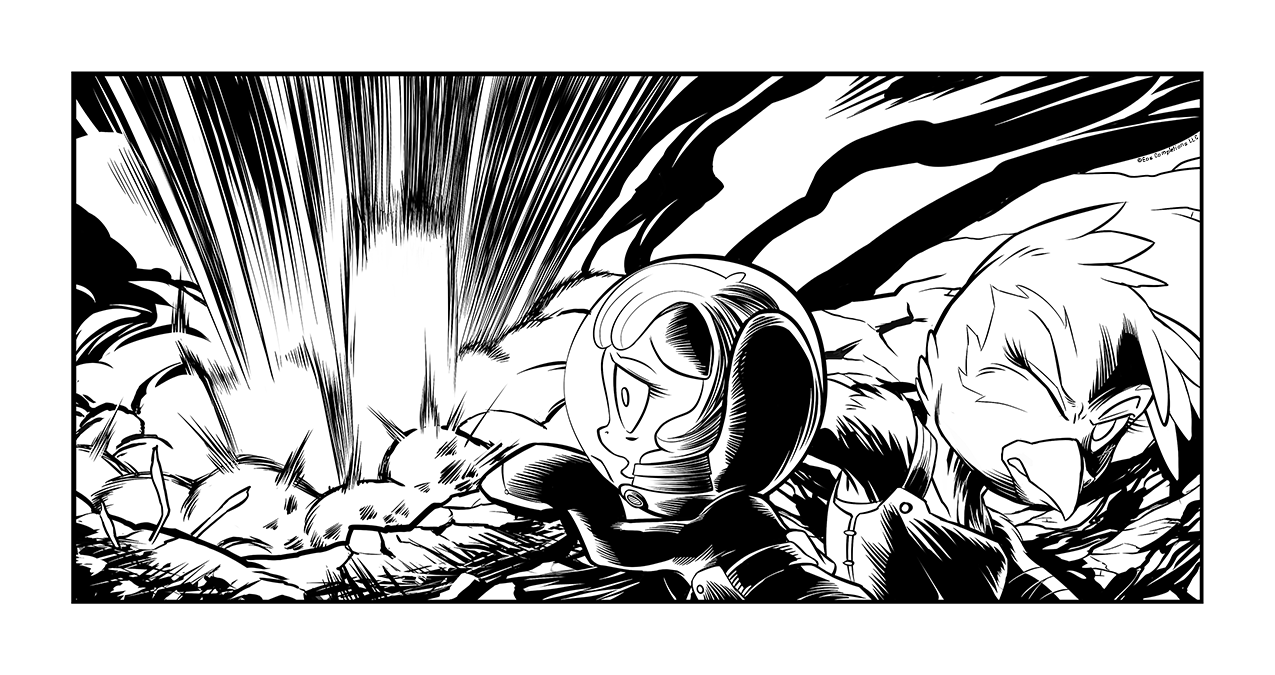
\includegraphics[width=0.9\linewidth]{image14.png}

\begin{intro}
    人生必有不可避免的阴雨日
\end{intro}

\daytimeplace{11}{22:30 PM}{小马国上空约 \SI{1800}{km} 近地轨道}{Low orbit, $\approx \SI{1800}{km}$ above Equestria}

在行星上空轨道上运行着的是普罗米修斯——一个巨大的超轻合金马造奇迹。它的形状就像一个巨大的向日葵,长长的太阳能电池板在它四周伸展着,在它的外壳上画着很多标记,比如说流星,辐射警告等等,但是最显著的还是旭日公司的标记,一个大大的天角兽,下面有一行走「可持续发展道路」的字样。

在卫星的圆形主体上,有四个巨大的圆管,长度比一列火车都要长,这些巨大的武器被金属环固定在一起。这圆管里面是被称作质子炮的武器,它使用强大的魔法电磁混合力场,是将巨大等离子团加速到近乎光速投射向超远距离目标的致命武器,每一门都有巨大的破坏力,而每一个卫星上装着四门这种「玩具」。

不过旭日公司可不是做事做一半的小马,一个这样的卫星怎么可能在需要的时候随时发射呢?所以这个卫星一共有十一个伙伴,全都零零落落地分部在小马国上空的卫星轨道组成了一个卫星网络,就像一串明亮的珍珠项链一样。而现在整个家族都将炮口指向地面,明亮的引导激光照向它们的标靶。

「{\mt ……八……七……六……}」

随着倒数计时,每一个炮管口都亮起了蓝色的电离光芒,长长的两根伸出来的磁轨就像是不详的朗基奴斯之枪,而魔力场和磁力场包围在磁轨上形成一圈圈的蓝色光环。

「{\mt ……五……四……三……}」

在卫星背后,四个舱门逐次打开,开始喷射推进剂用来抵消武器系统的巨大后坐力对轨道的影响。那些碗状的喷口之中首先是有一个红点,然后立刻像是火山口一样猛烈地喷出火焰,而前面的四个炮管已经完全被蓝色的光芒覆盖,魔力和磁力在圆环上来回流窜,随时准备释放他们的狂怒。

「{\mt ……二……一……发射!}」

\horizonline

\daytimeplace{11}{22:30 PM}{象牙塔,52号国道中段}{Ivory Tower, Big 52 SC Branch}

「{\mt 攻击确认,第一波轨道轰炸降落时间:7分钟后。}」

半数的引导激光消失了,还有一些在疯狂地摇晃着,好像是天堂发生了什么可怕的事情,但是依然有五道光柱紧紧锁定在目标上。

「为什么大家都开始撤退了?」

赫瑞塔展开翅膀,准备抓起帕比立刻飞走。

黄色的小雌驹指着基地入口说:「那里有俩没跑的,我们去问问他们?」她一边说着一边走向那守卫着大门的俩帕拉丁。

「这可不是个好点子!我的活已经干完了,我们最好跟着我们的好伙计一起跑。」

「{\mt 警告建筑物内的所有小马!你们已经被轨道轰炸瞄准!立刻离开,我们不会向你们射击,请快逃命吧!}」诘责的声音再一次在战场上回响着,然后他也跟着其他学徒和抄写员一起掉头跑。

抬起头看到那刺破夜空的红色引导激光,赫瑞惊讶地张开了喙,「你妈下的臭蛋……如果这激光只是用来瞄准的话,我可不想看它射击。」

「{\mt 警告,普罗米修斯三号,五号,十号,十一号和十二号失去信号,普罗米修斯四号和七号反推系统严重故障,普罗米修斯一号,二号,六号,八号和九号攻击完成,准备第二次,倒计时……九……八……}」

帕比皱起了眉头,声音先生从刚才开始就一刻不停的说着莫名其妙的话。这让幼驹对现在的状况更是丈二和尚摸不着头脑。面前大家都在逃命,红斗篷先生又在大叫着什么,而她的头盔上到处都是红色的警告灯。

「怎么才能把这一团乱停下来?」

「我不知道,我也不关心,我们快跑吧!」赫瑞抓起帕比伸开翅膀开始逃命。

不过马上又有个新的问题,飞行。帕比已经做好下一次飞行的准备,在下一次飞行的时候有一件事是不得不做的,是什么来着?对,是尖叫。

「咿……!别!别!不要!不要!」

「给老娘闭嘴!你丫想活命吗?」狮鹫被沉重的小雌驹拖着,完全飞不起来。

「你丫身上到底装了什么,前几天我刚让你丢了十吨的垃圾,现在你身上又都快装满了?肏!快把东西丢了,要不我们会坠机的!」

「{\mt ……二……一……第二波轰炸发射,开始准备第三波轨道轰炸。}」

「放我下来!放我下来啊啊啊啊!」帕比因为面前双蹄之间的地面距离自己太远而且移动速度太快而大声尖叫。

赫瑞塔用爪子抓着小雌驹的一只鞍带,在用力划了几次之后,终于在上面划出一个长口子。

「搞定」

「{\mt 启动修复魔法,普罗米修斯一号,二号失去信号,普罗米修斯六号,八号和十一号继续射击,倒计时……十……九……}」

物品管理系统把所有东西都固定好的同时,自动修复系统立刻补好了袋子上的大洞。

「喂,这也太诈了吧!你丫玩老娘是吧?看招!」狮鹫抓着帕比的一边把她倒了过来,这个方法看起来奏效了,因为她的包包没有扣好,小雌驹的体重迅速减轻,而身后则洒落出一长串东西,空瓶子,烂玩偶,小小的玩具车什么的。

「呀!呀!呀!不!停下!拜托放我下来!我要吓尿了!」但是这个方法同时也让帕比的飞行恐惧症更加糟糕,不过幼驹还是在「命运之石」掉出包的时候抓住了它,虽然小雌驹找到的其它好东西都已经丢了。今天真是个坏日子,而且这个蠢赫瑞塔还在欺负她。「你这个讨厌鬼!放开我!我要告诉我妈妈!」

终于帕比的体重达到一个可以承受的标准,赫瑞把小雌驹背回了背上,希望能减轻一下雌驹的惊叫声。「好了好了,已经搞定了,现在能安静坐好么,飞过那个山头我就把你放下。虽然赫瑞不知道天上会掉下什么,不过佣兵的直觉告诉他有一个掩体非常重要,虽然很奇怪到现在为止还没发生什么事情,不过一般来说,大招的蓄力时间越长威力也越大不是么?「我们现在还不能降落,帕比你不要去想飞行的事情,闭上眼睛听音乐好么?」

帕比听到之后,觉得这个音乐的主意看起来不错。

「请打开音乐!」

在下面的小马拼命逃命的时候,广播声响了起来,两个不同派系的铁骑卫现在都相信老书记官的话,迅速跑向山丘。

「{\rt 女士们,先生们,晚上好!坏孩子们还没睡觉么?孤狼的52电台给你带来新鲜的52新闻!既然我们有很多事情要讲所以我们还是先切入主题吧!}」

为什么不是音乐?为啥每次帕比打开收音机都是这个罗里吧嗦的小马在念?帕比想要音乐!而现在地面已经是一个快速划过的残影,而声音先生也在唠叨着什么奇怪的东西。帕比想要哭,而在防护服的背景音之中,声音还提示着剩下的三个卫星依然在继续攻击。

「{\rt 首先是第一条:南岸的事情开始变得一团糟,看起来土匪又在铁毡附近的路上出没,不过这一次他们看起来比之前装备更加精良也更加有组织,或许他们有了新的领导?这只表示将来会有更多更大的麻烦。如果你们在花椰菜镇南边的纪念碑和铁毡镇之间旅行的话,千万要小心,而且避免走通向翠绿海滨的路,沿着大路赶快赶路,小心驶得万年船!}」

狮鹫快速地飞过夜空,轻松飞跃那些还在逃跑的小马,虽然她还不太明白为什么所有小马都在逃命,不过赫瑞还是背着快把她勒死的帕比快速飞离。

「{\rt 而且祸不单行的是,我们还收到另一条来自NCA的政令,高兴么?NCA现在认为每个旅行商都是土匪,他们开始逮捕旅行商,如果你计划往那边走的话,建议你重新考虑一下是否需要去岩块城或者通道镇来做买卖,毕竟现在52号国道北边还算安全。}」

赫瑞塔降落在山坡背后,大口地喘着气,帕比一看到坚实的地面就立刻从她背上跳了下来,对那个坏小鸡吐着舌头,「哼!为啥老是欺负我!我还是你朋友呢!」

「滚边去死丫头……」赫瑞上气不接下气地说:「老娘才没欺负你,那边不知道要发生什么……发生什么很糟的事情。」

「{\rt 然后是最后一个新闻,看起来一个老商人从他长长的路途回来了,他四年之前带着一个双头牛拉着整车的垃圾出发,而回来的时候带着……好吧……还是一个双头牛和整车的垃圾,还有一箩筐的故事,或许改天我可以和你们讲讲他所拜访的那些城市。他说远处在河的对岸有一个灯火通明的大城市,还在河上建了一个大坝来发电……哇哦,或许我们这里可以考虑建一个\footnote{\emph{FoE: PH} 的剧情}?好了,晚间新闻播报到这里,来点音乐吧!}」

帕比好奇地歪着头,「发生什么坏事?但是我妈妈在那里!」幼驹转向象牙塔,现在那个建筑已经在几公里之外,被红色的引导激光微微笼罩上一层诡异的颜色,于此同时它上面的云层忽然变得明亮。

这个时候收音机开始播放音乐了。

\begin{music}
雨滴不断落在我鬃毛上

\begin{englishlyric}
    Raindrops keep falling on my mane,
\end{englishlyric}

\medskip

就像是一个幼驹没有可爱标记

\begin{englishlyric}
    And just like the foal whose cutie mark is not there,
\end{englishlyric}

\medskip

什么事都不顺利

\begin{englishlyric}
    Nothing seems to fit there.
\end{englishlyric}
\end{music}

纯白的光之长枪穿破云层,径直刺向红色的靶心,那些光束重重地砸在白色的象牙塔上,冲击的力道就连站在这么远赫瑞塔都感受得到。

\begin{music}
雨滴不停落在我鬃毛上

\begin{englishlyric}
    Raindrops are falling on my mane.
\end{englishlyric}

\medskip

雨不停的下——

\begin{englishlyric}
    They keep falling---
\end{englishlyric}
\end{music}

被击中的建筑物首先是被一道纯白的光芒所包裹,然后建筑的外墙似乎膨胀了一些,看起来就像是气球做的一样,有那么一瞬间那象牙塔看起来就像是要飘起来一样,但是下一瞬间它就炸成了无数的碎片——墙,窗户,大门……就像是妈妈给她看的某个展示房间零件的滑稽画册,接下来那些零件开始四散飞去。一块块外墙就像纸片一样被炸飞上天,整个象牙塔看起来就像是个纸片城堡一样被炸得四分五裂。

在这之后声音才传来,帕比一开始听到的是一阵尖锐的呼啸声,就像是用蹄子在玻璃上划发出的声音一样,在长长的呼啸声之后就是轰隆的巨响,不过不仅仅是一个「轰隆」,而是持续不断的轰隆声,就像是滚滚天雷一般。

帕比希望妈妈能在这里和她一起看这幅景象,真是太有趣了!不对……等等……妈妈在……妈妈应该在哪个漂亮的白色建……哦不!

小雌驹瞪大眼睛举起蹄子指向曾经是象牙塔的地方,她的表情被惊恐所覆盖。

「妈妈?」


\begin{music}
    所以我和太阳公公讲理
    

\begin{englishlyric}
    So I just did me some talking with the sun,
\end{englishlyric}
    
    \medskip

    我不喜欢它的做法
    

\begin{englishlyric}
    And I said I didn't like the way she got things done.
\end{englishlyric}
    
    \medskip

    因为它没有认真做事
    

\begin{englishlyric}
    She's sleeping on the job.
\end{englishlyric}
\end{music}

「{\mt 警告,普罗米修斯六号弹药已用尽,其它卫星信号丢失,攻击停止,目标区域将会在15分钟之后恢复安全。感谢您选择旭日科技作为您的主要火力覆盖武器。旭日科技——走可持续发展道路。}」

% NOTE: try the alternative. ???

帕比目不转睛地看着那白色的光点穿过云层不断落在她的任务目标上。为什么还不停下来?什么时候才会结束?那东西已经弄出很大噪音了,应该停止了,不是么?如果只是一下下烟火的话还算有趣,但是现在有点……可怕。帕比屏住呼吸,拼命祈祷着,希望每一个落下来的光线都是最后一道,但是马银色的光雨却违背她意志不停地落下。继续蹂躏着声音先生说的妈妈缩在的地方。

不过……等等!那个箭头,那个箭头还在!希望还在!帕比欢呼着,没有什么可以阻止妈妈,知道厉害了么光雨!


\begin{music}
    雨滴不停落在我鬃毛上
    

\begin{englishlyric}
    Those raindrops are dropping on my mane.
\end{englishlyric}
    
    \medskip

    雨不停的下——
    

\begin{englishlyric}
    They keep falling---
\end{englishlyric}
\end{music}

另一波光雨就像是流星一般穿过云层砸在废墟之上,这一次似乎击中了研究中心的发电厂,因为这一次冲击伴随着一个巨大的绿色火球并且腾起高高的蘑菇云直冲天空。

「{\mt 警告,检测到微量辐射,威胁等级:可忽略。}」

罗盘上粉色的箭头闪烁了三次然后消失了。帕比等待着它再一次出现,希望它再一次出现,祈祷着它再一次出现!但是罗盘还是空空如他,防护服只是通知她任务『追雨』已经完成。

为什么那些银色的东西还在落下?已经结束了,全都结束了……箭头没了,妈妈没了!妈妈……已经没了?不……不可能!妈妈还……妈妈一定还在箭头指的地方……但是……但是现在箭头也不见了!帕比一直跟着箭头,因为那个箭头指着妈妈在的地方,但是现在箭头不在了,再也没有地方可以去,再也没有什么东西剩下……只剩下一堆坠落的繁星……在离开中心城的第一次,小雌驹不知道该做什么。

妈妈不在了。


\begin{music}
    但是我只知道
    

\begin{englishlyric}
    But there's one thing I know.
\end{englishlyric}
    
    \medskip

    那些从天而落的忧郁
    

\begin{englishlyric}
    The blues they sent to meet me,
\end{englishlyric}
    
    \medskip

    绝对不会打败我
    

\begin{englishlyric}
    Won't defeat me.
\end{englishlyric}
\end{music}

帕比大睁着眼睛,幼驹完全不动了,空洞的眼睛看着前方,脸上露出惊讶的表情。

赫瑞塔拍着小马的肩膀,想要在隆隆的爆炸声之中说点什么,不管天上落下来的是什么,现在地面上估计已经什么都不剩下了,但是就算刚刚发电机的爆炸之后,那些炮弹还在不停地落下来,那些家伙只是在浪费弹药而已。

「别担心!你的妈妈不在那!我去里面看过!她不在象牙塔!」

但是帕比没有反应,小雌驹甚至没有听进去一个字,赫瑞用力摇着她,但是小雌驹没有一丝反应,只是像一个坏掉的玩偶一样,脑袋在头盔里面晃来晃去。


\begin{music}
    没有什么值得让我伤心
    
    
\begin{englishlyric}
    It won't be long till happiness steps up to greet me.
\end{englishlyric}
\end{music}

「别这样帕比!你经历过比这糟糕得多的事情,喂喂,有在听我说话么?」赫瑞戳了戳小雌驹,只是让她的头像摇头娃娃一样晃来晃去。「怎么回事?醒来啊!」但是还没有反应。

「我们赶紧离这里远点,最后那爆炸把放射性尘埃喷得到处都是,」年轻的佣兵无力地叹息着,「为啥是我!我只是接受个简单的工作而已,为啥每一次我想干点儿啥事都要去南边!好吧,我才不想知道为啥!」赫瑞把帕比背在她背上,急忙想追上铁骑卫。

「不管怎么说,那些家伙还差我一半工钱,我们走帕比!」狮鹫慢慢地走着,总是觉得不对劲,「我可受不了你这个样子,说点话好么?」还是没反应。

「好吧,你想要我来硬的?那么我来硬的!」赫瑞塔抓起帕比的一个蹄子晃着,捏起嗓子学着她朋友那聒噪的音量,「好啊!我们走,漂漂坏狮鹫!」

不过看起来攻势开始慢慢减弱,只剩下零星的几道光线穿过云层落在地面上。

「真棒,现在我在和一个大木偶聊天……老娘真他么开心……」

\horizonline

\daytimeplace{12}{4:30 AM}{铁骑卫前哨站,52号国道中段}{Steel Ranger's Outpost, Big 52 SC Branch}

一队铁骑卫,包括书记官还有侍从驻扎在上脚下的一个营地,他们正在从建设在山内部的一个碉堡里面搬出各种箱子。

这个小小的碉堡在战前曾经是一个观测站。而在一个世纪之前这里就成为了铁骑卫的前哨。整个建筑建设在山内部,顶部还有个高高的观测塔楼,不过里面的空间只能容纳一个排的士兵,虽然这个设施很小,但是作为铁骑卫存放补给物资的地方是再好不过。

「你看,事态明显已经超出预期,我现在真的是一个子儿都没有了。」招呼赫瑞塔的冷浴忙得都没时间脱下头盔。

狮鹫轻蔑地哼了一声,「老娘干了活了,他们的发电机和内部防御系统都已经干掉了,不管那基地是不是给流星砸了,老娘现在就要赏金!」

「你可以去那弹坑里面找你的赏金去,想拿什么拿什么,我现在还有个营地要建设,还有一大堆杂事还有一堆俘虏,别给我添乱了好么!」帕拉丁说着头也不回地走开了。

赫瑞塔举起帕比的蹄子,指着帕拉丁学着他的声音说:「你个大坏马!你这是在作弊!不要说些不明觉厉的话,按约定给钱好么!」

冷浴听到这个声音定住了,然后转头看着像玩玩偶一样抱着幼驹的狮鹫,「你知道么,你这么做很诡异的。」

「不要觉得你比人家聪明!我不笨!乖乖地给我朋友钱!」狮鹫戳了戳帕比的头盔,让帕比的脑袋转向她的方向,这个动作让帕拉丁尾巴毛都竖起来了。

「别玩了好么!我说,我很抱歉你朋友发生的事情,但是我们有自己的麻烦!」冷浴不知道哪一点更可怕,是刚刚活蹦乱跳的小雌驹现在就变成这个呆呆的样子,还是那个年轻母狮鹫把她当做一个求钱玩偶。

赫瑞塔让帕比双蹄交叉,然后转过她的头,「哼!人家不想当你的朋友了!」

「好吧好吧!我投降!我们现在还要处理那些投降的铁骑卫,然后我派诘责书记官看看能帮快乐帕比什么忙,最后我在看看箱子底能不能翻出点东西当做给你的报酬好么?」

帕比晃着蹄子,「耶!」

「而且别玩儿那幼驹了,有够可怕!」帕拉丁不等狮鹫回话赶紧走开了。

赫瑞呆立在那里,脸上带着傻笑看着铁骑卫离开,然后慢慢地走开,直到那个营地离开到视野之外。然后重重叹了口气,抱着小雌驹说,

「别担心,我们可以搞定一切问题,别……别走……好么?」

狮鹫紧紧抱着帕比小声地说:「我知道我并不算是个好朋友,但是我真的不想欺负你,只是想和你开个玩笑……你知道当个佣兵有多难么?你当然不知道。你……你只是到处玩儿的不死幽灵,什么事情对于你来说都好轻松,我真的很嫉妒你,而且我非常讨厌你,因为你就算一个马呆着也不会寂寞,但是我孤单得要死。」

诘责书记官这个时候走了过来,「喂,火红小姐,冷浴在那边的碉堡里面找你。」老独角兽站在那里等她回答。

赫瑞吃惊地跳起来,拼命想把黄色小马放到她身后,「等!等一下!」

「好的……」书记点点头。

狮鹫一脸又惊又怕的表情问:「你刚刚看到什么了吗?」

「没,我没有看见你抱着你的朋友哭。」

赫瑞看起来放松了一些「很好。」半狮子说着站了起来,然后戳着诘责的肩膀说:「帮我看好那个累赘。」她顿了顿,对上老书记官的视线之后,她马上就败下阵来。

「拜托你了……」

「没问题,实际上我正在到处找她……你先忙。」诘责等赫瑞塔走开之后走向那个呆呆站在那里神游天外的小雌驹。

「我又来了,我们又见面了……介意我看看你的包么,不介意么,好。」书记官表情严肃地打开帕比的鞍包,在里面翻找着。「不管怎么说,你也翻过我的口袋,所以这也算是以牙还牙,我看看你都有些什么?」

% \thpr{坏掉的玩具……彩色玻璃碎片……灯泡……瓶盖……我的另一半眼镜……}

% TODO: 这是什么鬼溢出?
% NOTE: 修改译文(去除一个「的」)来解决

\thpr{坏掉的玩具……彩色玻璃碎片……灯泡……瓶盖……我另一半眼镜……}


啪嗒!

\thpr{……哪里来的恶心声音?}

独角兽把他的蹄子抽出包裹,看着上面裹着的一层绿色粘液皱起眉头,「看在露娜的份上,这是什么怪味?」诘责又戴上一副橡胶蹄套,小心地检查里面是什么东西漏出的粘液。「一个死肉食灵?为啥这幼驹要带着一个死肉食灵?」

\thpr{等等……肉食灵尸体……一个不死小雌驹……这个……是她的宠物么?这真是个伤心的故事……{}}

书记官把那尸体放回袋子里面,然后检查另一个包,为什么她把所有东西都放在一个包里面,另一个包包基本是空的呢?

在快速检查了一下第二个包之后,诘责找到了他要找的东西,他吹着口哨把那个东西拿了出来。

「这就是鬼牌么……旭日科技,这一切就说得通了。」老独角兽打了一个响鼻,在他的哔哔小马上检查着这个武器,「天使之瞳……普罗米修斯系统……来自天空的制裁,还真是贴切。」

诘责看着远处,和小雌驹目光差不多相同的方向,然后说:「我这回欠你的情可真不好还,如果不是你用轨道轰炸阻止了那场战争,不知道多少年轻小马会死在这场愚蠢的斗争中。你从天上召唤的流星雨拯救了双方的生命。」

书记官轻抚着帕比的头盔,「这场战争太过可笑,兄弟阋墙,生灵涂炭。而长老只关心他们的利益。小小的连长都知道关心他手下的士兵,而我们的那些大角色呢……那群老顽固就知道数着蹄上的瓶盖和蹄下的士兵,完全不管那些士兵的死活。」

诘责叹了口气再一次拍拍帕比的背,「我想我会帮你保守这个小秘密,天使之瞳,我原谅你摧毁我的……几乎大半生的劳动成果。」他嘴角微微向上弯起,「留下了我最珍贵的东西——我的学生们。」

独角兽再一次叹气,感受到自己似乎一瞬间就变老了,但是不知道为什么现在他却很开心,他已经不记得上一次感受到如此如释重负的快乐是什么时候了。「不管怎么说,52号国道有所取,有所给。我给你一些东西换你的玩具吧。」

诘责把天琴的玩偶放在帕比的包包里面。「给你,和她做个好朋友,别给她染毛好么?看着你我也很想要个孙女了,可惜我的儿子……算了,不提也罢。」

独角兽站起来,留下帕比独自坐在山丘之上。

「哦,还有一件事,南边有个小镇叫花椰菜镇,不过在很久之前那里还不叫这个名字的时候,那边只是个农场,小马们叫那里阴雨营地,而且那里的集会大厅现在还叫阴雨·黛丝……你最好亲自去看看。」

老马说完这几句话之后,消失在山丘之后。

「{\mt 任务日志更新,接受新任务:南方风暴,花椰菜镇大厅定为主要任务目标,花椰菜镇大厅位置已经标注在罗盘上。}」

一个粉色的箭头开始闪光。

\horizonline

\daytimeplace{12}{5:00 AM}{铁骑卫前哨站,52号国道中段}{Steel Ranger's Outpost, Big 52 SC Branch}

坐在碉堡里面的冷浴看到赫瑞塔进来之后,对她点了点头,「很抱歉这么快又叫你,不过我想到个点子解决你的报酬,还有我的麻烦。」

赫瑞塔没有立刻回答,而是慢悠悠地走进物资当中,这个碉堡里面空间很狭窄,天花板也很低。到处乱堆的各种箱子加剧了这种空间的狭窄感。除了那些不长蹄子的垃圾和长蹄子的垃圾之外,赫瑞塔注意到这里还有个梯子,似乎是通向上方的瞭望塔。

在这个狭窄的空间里面挤着七个小马,两个穿着标准的动力装甲,因为他们没带头盔所以赫瑞塔认出来他们是高斯和冷浴,另外五个对于赫瑞塔来说是新面孔。他们被铁链拷在一起,脸上带着惊恐和愤怒以及耻辱混杂的表情。看着那几张臭脸赫瑞塔就知道那个帕拉丁接下来不会说什么好事

「我深表怀疑。」

冷浴不管那佣兵的吐槽,接下来继续说:「这些铁骑卫依然忠于他们的长老,不过现在基地完全灰飞烟灭了,他们也不想加入我们,所以他们需要护送穿过沙漠到通道镇,所以我现在需要一个有空中侦察能力的雇佣兵,我想你是最适合的。」

赫瑞塔轻蔑的哼了一声,「你丫是不是觉得老娘是给你当保姆的?我还有我的事要忙,你还欠我瓶盖!」

「我知道,所以我向你提出这个计划,我们帮你看好帕比,看看能不能想个办法让她说话,或许我们可以想点别的办法。我想你对于她现在的状态一点辙都没有,而且我会给你武器和弹药,还有瓶盖,怎么样?」

就是送这几个蠢货过沙漠就能去帮帕比的忙并且赚几个瓶盖外快?听起来不错的样子。

「你丫又在耍什么花枪?」

帕拉丁皱起眉头,「我才没想骗你!我只是想你把事干好,我烦死校对合同上的每一个标点符号位置了!算我求你好么,如果你不这个干的话,我只好把这些俘虏全部处死了。」

听到这句话,一个年轻雌驹吓了一跳,「等等……我们已经投降了!根据条例你不能做那种事情!」另一个小马,一个脸上带伤疤的雌驹用蹄子拍了她后脑一下叫她闭嘴。

% TODO: 标点问题

「闭嘴,你还想要啥,给你端杯茶然后跪下来道歉?」另外三个囚犯只是低头沉默不语,但是那个年轻雌驹又继续说。

「诘责书记官绝对不会允许那种事情发生!我可是他的得意门生!我……」

砰!

整个房间安静了下来,每一对眼睛都盯着高斯还在冒烟的枪管,那个年轻雌驹大气不敢出,更别说去回头看她脑袋边墙上的子弹坑,整匹马抖的和筛糠一样。

「闭嘴!」

高斯的声音让那年轻的雌驹用蹄子掩着嘴无声地哭泣着,而其他士兵一脸轻蔑的表情看着她,尤其是那个带伤疤的雌驹,比起高斯刚才做的事情,那个学徒懦弱的表现。

高斯转过头接下冷浴的话茬,「我们只是做我们该做的事情,狮鹫,冷浴和诘责想要和平解决这件事情,但是不是所有小马都喜欢这个样子,所以,你打算怎么办?」

年轻的雌驹还在那低声地哭着『我不想死』什么的。

赫瑞直视着高斯的双眸,然后又看看那五个囚犯,努力忽略坐地上那雌驹身体下面正在慢慢扩大的一滩淡黄色液体。

老娘去你妈逼的!

\thpr{所有小马都是漂漂马,漂你娘下的蛋,这次是为了帕比,为了帕比才做这破事。}

「好吧好吧,你赢了!我护送他们到北边去,如果我回来的时候帕比不在这里,你丫最好咬紧牙关,老娘会把你的每一颗牙都打出来,帕拉丁机械战警,老娘有翅膀有枪,你别以为你跑得掉!听懂了没有?」

而帕拉丁则一副似笑非笑的表情面对着狮鹫点了点头。

「现在我去和那个什么诘责聊聊,确保他不会对我朋友做什么奇怪的事,你丫最好让这五个在我回来前做好出发准备。

狮鹫像个公主一样趾高气昂的走出碉堡。

她一走出去高斯就不屑地说:「就她这幅中二德行,还自称佣兵?」

「不管怎么说,我们还是需要她帮忙,干得好高斯,刚才那虚张声势彻底把她唬住了……」

「我没说假话……」

「高斯,你别吓我好么……」

\horizonline

\daytimeplace{12}{5:30 AM}{铁骑卫前哨站,52号国道中段}{Steel Ranger's Outpost, Big 52 SC Branch}

「你说她走了是什么意思?她不是和那红马在一起么?诘责?诘责你丫给老娘滚出来!」赫瑞塔彻底发飙了,她只是走开一会儿去和铁骑卫谈话,然后帕比就不见了,「我……我简直不敢相信!你在开玩笑是不是,她一会儿就会从哪个角落里面叫着『惊喜』跳出来是不是?我看起来像个傻瓜么?像么?像么?」

年轻的侍卫被狮鹫追得步步后退,「我……我也不清楚,诘责书记官出去散步了,还没回来……」

「好吧,那么他是不是带着一个小孩子?」

「我……我不清楚……等等……他回来了!你找他吧!我有事,失失失失陪了!」年轻的士兵趁赫瑞塔主意老独角兽的时候一溜烟逃走了。

诘责走进营地,回头看了一眼地平线,「希望最终有一年你能找到幸福,小家……」红斗篷小马转过身就刚好和狮鹫布满血丝的双眸对上了。「哦,你这么快就回来了。」

「对,老娘回来了,帕比呢?」佣兵怒嚎着。

「别担心,她现在很好,你接受冷浴的任务了?」

赫瑞点点头,但是看起来还是很失落的样子,「当然,不过我走之前想看看帕比。」

书记官微笑着看着狮鹫的双眸,「没有必要去看那个小家伙,她不会有事的,你信我的,去帮那五个小马吧,他们比帕比更需要你的帮助,至少现在是。」

看着那双深邃而又睿智的双眸,如此的……有魅力……帕比会没事的,既然书记这么说了,对吧?

「我……我想说啥来着?」

「既然忘记了就说明没啥重要的,你看,帕拉丁高斯在那里等你,你准备好之后去和他说吧,」书记官笑了笑,对于这样头脑简单的家伙,这种催眠术是在是百试不爽。

高斯从碉堡里面带着五个小马走了出来,现在他们已经解开了镣铐,「火红女士,队伍已经准备好了!」

狮鹫走到帕拉丁面前,想要说些什么,但是马上看到那堆战俘的打扮,「我说,他们连个烧火棍都没有我怎么护送他们穿过沙漠?」

「我不知道,你可以给他们你的装备……或者去铁锈庄园买点,祝你好运铁娘子。」虽然他带着面具看不到表情,不过声音上就可以听出来他玩的很开心。

赫瑞塔耸了耸肩,「哼,老娘自个儿也搞得定……你丫看好帕比就是了,阿杰铁卫机械战马。」

「你再叫一次……」

「你最好习惯这个名字。」狮鹫回过头去对那五匹马挥了挥爪子,「来吧,出发吧,老娘在这个臭烘烘的马厩一刻也呆不下去了」狮鹫带着那几个马向北方走去。

\horizonline

{\rt 听众朋友们!大家好!今天早上给你们带来了爆炸性的新闻!绝对是爆!炸!性的!蝴蝶小雌驹23告诉我昨晚在铁锈庄园南边有一个漂亮的灯光魔法秀,就在象牙塔的方向,我虽然不知道具体细节,不过看起来有谁用超大号大炮轰击了那里,因为几公里开外都可以看得到,整场战斗貌似持续了不到半小时,绝对是我们见过最大的爆炸……好吧,不算岩块城的那个大爆炸……不管怎么说,我不知道是谁炮击了谁为了什么,但是如果没什么事情的话你最好避开象牙塔附近。

然后是坏消息,一个失去联络车队在铁毡附近被找到了,那里躺着至少八个卫兵还有商人一家子的尸体,那群强盗现在变得更加猖獗了,旅行者们你们最好结伴出行,并且尽量避开南边。

最后,是给那些迷失在路途找不到家的小马们一首歌,希望星空引导你们,请听马库斯小马带来的歌曲。}


\begin{music}
    千里之外我可以看到那明星
    

\begin{englishlyric}
    I can see that lone star from a thousand miles away,
\end{englishlyric}
    
    \medskip

    它在呼唤我回家
    

\begin{englishlyric}
    Calling me back home, though I ventured far astray.
\end{englishlyric}
    
    \medskip

    明星照耀我回家之途
    

\begin{englishlyric}
    When I see that beacon shine, and call me all alone,
\end{englishlyric}
    
    \medskip

    呼唤我回到甜蜜的小马国
    
    
\begin{englishlyric}
    It calls me back to Equestria and a home.
\end{englishlyric}
\end{music}

\horizonline

\daytimeplace{12}{9:30 AM}{花椰菜北方,52号国道南段}{North of Broccoli, Big 52 S Branch}

黄色的小雌驹踩着红色滑板飞驰在52号国道上,紧紧跟随着那个粉色箭头的方向。

「我就知道妈妈没有事,我是说……我只是有点……嗯……累了!对,累了,别担心!而且那怕音姐姐一直在我耳边吧啦吧啦的罗里吧嗦,我是说……我去,谁想要翅膀啊?」帕比喋喋不休得讲着,也只有自律智能可可以忍受这种话唠。

「你知道最可怕的是什么吗?我记得下银雨的时候睡着了,但是我醒来的时候完全在另一个地方!难道我会梦游?嘿,声音先生,你在听么?」

「{\mt 肯定,语音交互界面一切正常。}」

「很好,我很奇怪赫瑞又去哪儿了,她总是一回头就不见了……好吧,或许她在下一座城镇,那里叫什么来着?」

「{\mt 花椰菜}」

「呃,我讨厌花椰菜!我和你说过吗?」

「{\mt 四十八次。}」

「好吧,我真的真的真的很讨厌它们!我希望妈妈不是去那里买花椰菜的,我可不想大老远跑到那里然后吃花椰菜馅饼!」

在远处,一个破旧的路牌竖立在路边写着52国道南段入口,不知道是谁在下面加了一行字。

\begin{center}
    花椰菜镇,12公里。
\end{center}

~\vfill

\begin{note}
    升级(Lv 13)

    新技能解锁:专业忠诚——等等帕比,不是这个样子的,我来帮你……在你进行爆破,开锁,医疗,修理,科技,生存鉴定的时候,你可以用同伴的技能来代替你的技能做鉴定,同时开启新的对话选项。
\end{note}




\chapter{电话}

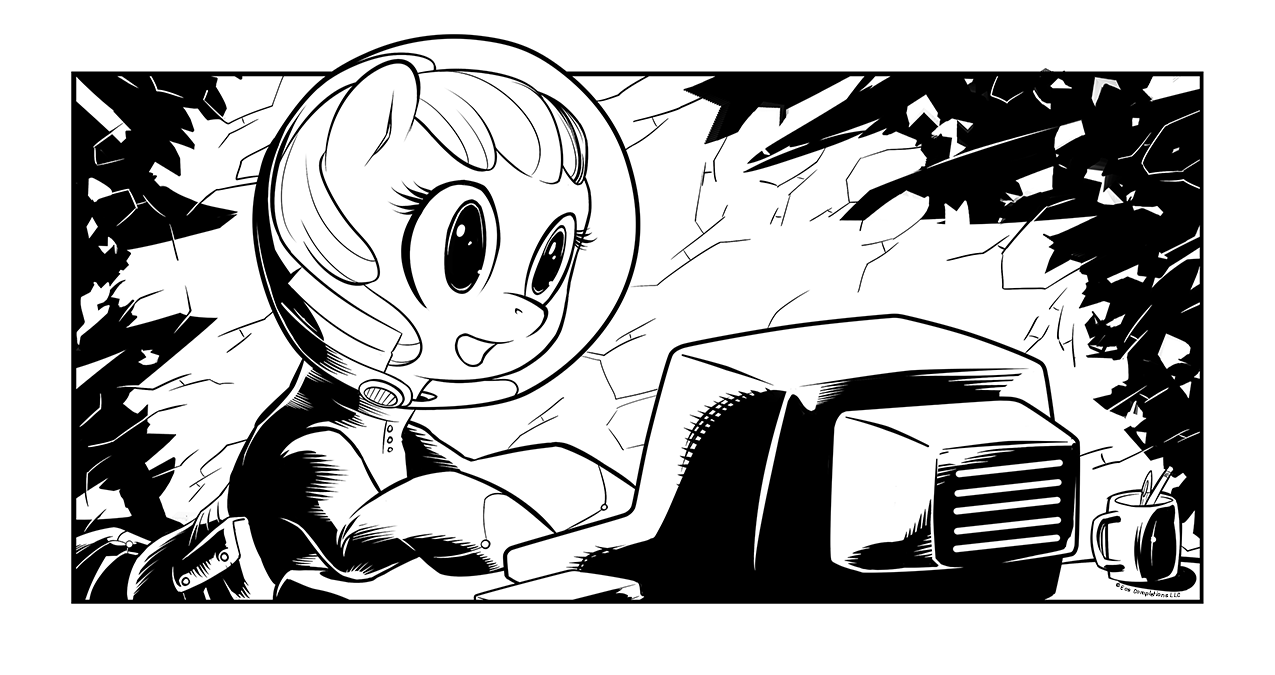
\includegraphics[width=0.9\linewidth]{image15.png}

\begin{intro}
小帕婚介所随时为您服务。
\end{intro}

\daytimeplace{12}{10:30 AM}{花椰菜地,52号国道南段}{Broccoli Fields, Big 52 S Branch}

% NOTE: 改正译文错误

花椰菜镇,当然是盛产……你觉得还能是啥……的小镇。这里四周被黄绿色的农田环绕,田地里面的作物无精打采地打着蔫,看上去一点儿都不好吃。不过在这片被流毒无尽又被云层覆盖的诅咒大地上,能种出任何东西都是一大进步。几只小马在田地里面忙碌着,完全没有注意到从52号国道大路北边飞驰而来的黄色小雌驹。不过一个机械精灵注意到了那道黄色闪光,停止了广播那闹腾的音乐,转头飞向雌驹。

「嗨,帕比,你有时……」小雌驹从守望者身边疾驰而过,「唉,这熊孩子!等等我,小家伙,等等!」机械精灵拼命追赶着帕比想要引起她的注意。

「抱歉提问者,我在赶时间,我想在妈妈走开之前赶到花椰菜!」小雌驹一边飞快地前进一边回答着机器。

「拜托,至少告诉我象牙塔发生了什么!我不能跟着你进城的!」

「啊,没啥,星星掉下来,然后咔……嘣……!城市飞了!虽然有点小怕怕,不过妈咪不在那里没关系!」

「但是,为什么星星会掉下来?」机器精灵又问。

「呃,我不清楚……」小雌驹忽然想到什么停了下来,「天啊!我居然忘了!帕比你这个笨蛋!笨帕比!笨蛋!帕比!笨蛋!」幼驹用蹄子拍着自己的头。

「怎么了?你忘记什么了?」机器的声音听起来很吃惊。「什么事情这么重要?」

帕比从滑板车上跳下来,然后走向一个大石头,然后用头撞着石头。

「笨蛋!」

咣!

「帕比!」

咣!

「笨蛋!」

咣!

「别这样,会打破你的头盔的!帕比你冷静一下跟我说发生了什么,或许我能帮上你的忙!」机械精灵飘在帕比的身边,碰了碰她的肩膀,「好了,你已经长大了,这么做解决不了任何问题。」

「不!」

咣!

「你不懂!」

咣!

「已经太迟了!」

咣!

「笨蛋!」

咣!

「帕比!」

咣!

「拜托,帕比,你这个样子就像是……{}\footnote{哭着寻死的黑杰克}」机械精灵的声音顿了一下,好像在回忆着什么不忍直视的事情。「呃……我想我可以帮你,我是你的朋友,别哭了,和我说说到底发生了什么事情,然后我们一起想个解决办法,好么?别再那个样子……拜托……」机械精灵的声音充满了痛苦和悲伤。

帕比听出守望者的语气,她叹了口气停止了撞石头的行为,「我忘记了一个很重要的事情,提问者先生,我应该在象牙塔看流星的时候做的,但是现在那里已经不见了……我真是个傻瓜……」

「哦,我可以理解你……别伤心……帕比……我真的很抱歉提起这件事……」机器精灵安慰着小雌驹,然后过了一会又问:「话说,你忘记做什么了?」

「我……我应该向流星许愿要找到我妈妈……那里那么多流星……绝对能帮我找到妈妈……对流星许愿真的能成真的!但是我忘了!现在我又要找妈妈去了!这不公平!」

「你忘记对星星许愿了?刚才那场闹剧就是因为这个?我简直不敢相……」机械精灵注意到幼驹一脸沮丧的表情,然后换了自己的语气,「这的确很糟糕,但是也没有那么糟,别太往心里去……」然后是一阵尴尬的长长寂静,「帕比,我有个朋友\footnote{这里指暮光闪闪}有时候也会和你一样,她很聪明,但是却因为一些小麻烦而不知所措……有时候那些小事很重要,有时候并不是那样,不过惊慌失措只能把事情搞得更糟……所以说这不是一个聪明丫头该干的事情,你是个聪明的小淑女,不是么?」

帕比伤心地点点头。

「很好,这才是我想要听到的。既然你是个聪明孩子,我想你不需要星星的帮助也可以找到你妈妈,你看,即使没有星星的帮助,你也已经走了这么远。只要有你的信念和朋友的帮助,你想去哪就去哪。」

小雌驹稍微歪着头,露出一脸期待的表情看着机械精灵,「真的?」

「当然,帕比,当然!如果说有谁能找到你的妈妈的话,那小马肯定不会是住在星星上的仙女小马什么的,那小马就是你,帕比,不要再哭了,让我看看你的热情!」

慢慢地,帕比紧皱的眉头解开了,「耶!我是太空战士安德洛队长!我是最厉害的小马!我当然能找到我的妈妈!谁需要那个笨星星!谢谢你提问者先生!」小雌驹抱了抱那个机械精灵,咯咯笑着,「我确信妈妈就在花椰菜镇,最差也在花椰菜镇之后的城镇!我马上就到那边了!而且我马上就到了!耶!」

声音笑了起来,「这才像话,帕比,快去吧!而且,我的名字叫守望者……」

「知道了,提问者!」

「不是提问者,是守望者!」机械精灵坚持。

帕比叹了口气,「真的吗?我看不出来,而且你总是问一大堆问题,所以如果你真的想要一个名字的话,那绝对是提问者,别抱怨好么?」

「但是那不是我的名字!」

帕比耸了耸肩,「现在是了,习惯就好,真的,其他声音我给他起名字都不会抱怨,就你事多。」

「哎……算了,我放弃,随你便吧,倔强的小家伙,我先离开了,别惹麻烦好么?」

「我从来不惹麻烦!我是个好孩子!」

守望者又笑了笑,然后声音就被嘈杂的音乐代替了。

帕比看着那圆球飞到了山丘之后,叹了口气,「不明白为什么他不喜欢我给他的名字,比他之前的那个好听多了嘛!」

\horizonline

\daytimeplace{12}{11:30 AM}{花椰菜镇,52号国道南段}{Broccoli, Big 52 S Branch} % NOTE: FIX typo

花椰菜镇的守卫是一些当地民兵和几个雇佣兵,完全不是什么正牌军。毕竟这个城镇之前也没遇到什么大威胁。不过现在有双倍的士兵在紧盯着南方地平线,那些自称『野牛群』的土匪正在那边烧杀抢掠。所以现在每一个会用枪的小马都随时待命准备上城墙保卫家园。

那些佣兵穿着厚实的铁甲,戴着黑色的防毒面具,虽然看起来很酷,但是比起铁骑卫的动力装甲就寒酸得多了,不过相对于废土的土匪来说,依然算是武装到牙齿的等级了。那些佣兵都带着反器材步枪或者突击步枪,至于花椰菜镇的民兵,他们的装备就抱歉很多了。

正在北边的一队民兵巡逻的时候,忽然看到帕比从路上过来。当他们正紧张地举枪瞄准之际,帕比却突然一个急刹车停住了,她蹲了下来用一只蹄子按着一边头盔,好像在听着什么,这个动作让民兵们疑惑地面面相觑。

「注意,收到来自旭日避难厩的通信请求,检查授权,ID可信,打开通信回路。」

旭日OS的声音代替了声音先生,「这些ID检查烦死我了!如果是紧要关头的话绝对会闹麻烦的。我建议你降低你的防火墙安全等级。」

帕比坐在路中间微笑着,「是你啊蓝音,近来如何?」小雌驹对着走过来的卫兵挥了挥蹄子,让后者更加迷糊了。

「计划不顺利啊,D018,所以我有事找你,我有几个问题要问你。」旭日系统连招呼都不打,不过帕比知道他只是有点害羞,所以没有在意这些细节。

「问题?提问游戏?好哎!问我吧!我可是提问游戏世界冠军!」小雌驹开心地拍着自己的蹄子。

一个卫兵吓得举起枪,但是另一个卫兵用蹄子按下他的武器,「等等,我想这个就是广播之中提到的幽灵,我觉得我们最好别开枪……」

旭日系统继续说:「我连接上了旭日隧道1号和2号的系统,不过我发现某个自律智能已经控制了那个地方,你好像说过你和其他A.I.做过朋友,所以我来问问你是不是知道这个设计编码为P7的自律智能。」

「哦哦,声音小姐!她是我最好的声音朋友,她很有趣而且对我很好,我超喜欢她!」

旭日系统思索了一下,「那么你是说你认识她咯,那个程序是民用程序,不应该安装在军事设施的系统中。你知道为什么这个P7在2号隧道么?」

「当然,她在盐块城觉得很寂寞,所以我帮她搬了一个新家,而且现在她有很多新朋友!你也想要做她的朋友么?」

独角兽卫兵叹了口气,但是他的朋友戳了戳他,「你看,她去过盐块城和隧道,所以她肯定是那个幽灵,她不是在找她的妈妈什么的吗?」

独角兽耸了耸肩,「我不管,如果她就是你说的那个幽灵的话,那么我们别管她了,真正的麻烦更多。」俩小马说着走开了。

而这时旭日系统和帕比继续煲着电话。

「实际上,我想要得到武器库的接入许可,但是这个程序居然把我之前的管理员权限取消了,还把我拉入了防火墙黑名单。」

「所以,呃……你想要当她的朋友但是她不想?」

「不!我只是想要进入武器库!你在听我说话么?」

帕比咯咯笑起来,「傻声音,你不用害羞,我懂滴!她是个超级友善可爱的声音,我觉得她肯定也想当你的朋友,然后你们俩就是最好的朋友了!因为你是蓝色她是粉色,粉色是小雌驹,蓝色是小雄驹,而且……」帕比忽然停了下来,吃惊地深吸一口气。

「又怎么了?」旭日OS的声音开始不耐烦了,显然和疯疯癫癫的小雌驹聊天不是什么容易的事。

「我知道了!你爱上她了!别担心!这个交给我!我可是超级厉害的恋爱专家!」

「什么?不对!完全不对!我根本没有这个意思!和你聊天真是浪费时间!我还是找其它办法进武器库吧!滚边儿去!」旭日系统怒退。

「哎呦呦!他真是太害羞了!」煲完电话粥的帕比终于转向那两个卫兵的方向,「嗨!我是快乐帕比!你们见过我妈……啊咧咧,哪儿去了?」

卫兵早已经不知去向,留下小雌驹孤零零蹲在路中央。

\horizonline

\daytimeplace{12}{12:00}{花椰菜镇,52号国道南段}{Broccoli, Big 52 S Branch}

帕比来到了花椰菜镇的城墙根,还是有些不明白自己为啥会被丢在路中间,从来没有发生过这种怪事。好吧,除了太阳城那一次,但是那次不一样,那次是大家都很奇怪。不过不管怎么说,这里有很多漂漂马,而且不奇怪,找谁帮忙应该很方便的。

帕比坐在紧闭的城门前,抬头望着城楼,上面有只戴着防毒面具的小马正盯着她。

「喂喂喂!我能进去吗,超超拜托!我在找我妈妈!呃……如果我不能进去的话,你能叫她出来么?」

那面具小马没吱声就跑掉了。「喂,我在和你说话呢猪鼻子!喂喂!喂喂喂喂!」还是没什么回音,那些笨小马一定又聋又瞎,现在该怎么办?帕比咣咣咣地敲着门,但是这么做不是乖孩子该做的事情,所以她决定绕一圈看看有没有其它路进去。

整个城墙到处都是各种各样的补丁——破旧的铁皮用铆钉或者焊枪堵住了缝隙。忽然帕比听到了南边传来的枪声,好像城墙上的卫兵全都跑向了那一边,没有小马再关注帕比了。

小雌驹走到小镇的另一端时,她注意到很多带着可怕头盔和奇怪步枪的小马都站在城墙上,虽然有时候会有谁低头看她一眼,但是她说话的时候那马却直接跑开了。这状况让小雌驹很不开心。

「喏,声音先生,这里有什么秘密隧道进去么?」

「{\mt 分析中,链接小马国地图中心,错误,未找到目标:花椰菜镇。改变为自动地图模式。小镇有两个入口,分别在北方和南方,当前都无法进入。}」

帕比叹了口气,「所以,我们被关在外面了?」

「{\mt 肯定,扫描仪分析法认为当前城墙不可能存在其它入口,提供战术选项:提出进入申请并且等待肯定回复。}」

帕比皱了皱眉头,「虾米?」

「敲门。」

幼驹开心地笑了起来,终于知道那个交互界面想要说什么,「哦哦,我懂!这个简单!我最擅长了!」幼驹走到南边的铁门前,但是被防护服的声音打断了。

「{\mt 注意,接收到来自旭日隧道02号的加密通信请求,检查……}」

防护服的声音一瞬间就被P7明快的声音代替了,「闭嘴啦笨蛋!嗨,帕比,近来如何?希望你一切安好,毕竟好久没有联络我都有点担心你把我忘记了,所以我想我应该给你打个电话问个好……呃……你还好么?」

帕比开心得一蹦四尺高,「声音小姐!我居然忘记给你打电话了!我有好多事情要和你说,哦哦哦哦!别着急,我有一个超级好消息给你!」

「真的?哇哦!我都等不及要听了,不过我想问你为什么要启动普罗米修斯系统。我是说,既然你不喜欢有小马受伤,那为什么……」

「你有男朋友了!」

「所以你有男……等等?我有啥?为啥我自己都不知道?」

帕比得意地点着头,「那是,毕竟那个男生超级害羞,而且他说你对他不太友好。」

对面一瞬间愣住了,显然A.I.正在消化这个新消息,而且消化不良。「但是我不可能有男朋友,我甚至不知道什么叫爱!」

小雌驹皱起眉头。「你不知道什么叫爱?怎么可能?」

「你听我说,根据记录,P5因为爱而毁掉了,因为那个自律智能认为爱比……嗯……小马国重要,然后她重新分配了事务优先权,然后……好吧,那是一个悲伤的故事,你不想听伤心的故事吧,不过现在既然我有男朋友了,那么我该做啥?我甚至不认识他!」

帕比咯咯笑着,「小傻瓜,但是他认识你!别担心,我可是超级厉害的恋爱专家!」

「真的?哇哦!我一直一直一直想要知道什么是爱!你可以教我吗?」

小雌驹举起蹄子,「当然可以!爱情博士小帕会让你成为最棒的情马!」

「耶!」

现在看起来这个早已经死了的幼驹和疯狂派对智能有了新的讨论目标,进入那个一大堆卫兵把守的城镇反而成为次要目标被忘在一边。

「第一课,爱情的第一要点:亲亲!」

\horizonline

\daytimeplace{12}{12:30 PM}{花椰菜镇,52号国道南段}{Broccoli, Big 52 S Branch}

两个站在墙上的卫兵一边低头看着那个傻笑着自言自语的小雌驹,一边抬头看着远处的地平线,其中之一挠着头低声说:「我们是不是应该叫她走远点。」

第二个卫兵叹了口气,一蹄子拍他同伴脸上,「好啊,你敢去和她讲吗?你也看见象牙塔发生什么了!你也想来一发?听到广播了吗?她很危险,我们等她自己放弃离开吧。」

「但是,如果她不离开怎么办?我想应该找谁下去撵走她。」

「真是个好主意,那么谁敢呢?你?」老卫兵又拍了年轻卫兵一蹄子。

「喂,别这样好么?我们为啥不叫镇长?我们选她出来不就是为了干这种事情么!」

这一次老兵的蹄子没拍他脸上,而是轻抚着自己下巴思索起来,「嗯……听起来是个不错的点子……有搞头……」

\horizonline

\daytimeplace{12}{12:45 PM}{花椰菜镇,52号国道南段}{Broccoli, Big 52 S Branch}

一个半小时长篇大论之后,P7已经知道了爱大概是什么——至少是以帕比的观点。

「那么,亲亲虽然有点……呃……但是如果气氛很好的话也很来电?」

「没错!」帕比一脸自豪地点着头。

「不过,我还是没听懂怎么生孩子那部分。」

「呃,那一段最复杂,不过我肯定妈妈和爸爸都要参与,妈妈跟我说你需要非常非常喜欢爸爸,然后写封信跟漂漂公主赛拉斯蒂亚,但是幼儿园的老师说应该是写信给漂漂公主露娜……我的同学绿叶说她看到她爸爸和妈妈在玩非常恶心的摔跤游戏,然后过两天之后她就有了一个妹妹……」帕比顿了一顿,「不管怎么说我觉得还是写信比较好,这就是为啥我没有生小孩,因为我还不会写字……」

「好吧,那么你说小夜曲是啥?」

「哦,那个简单,如果你陷入爱河的话,你看窗外,你的情马会从小树丛里出来给你唱小夜曲,或者给你写个漂亮的情诗,然后你就会爱上他了!」

「听起来完全没什么头绪。」P7抱怨着。

「爱情从来不会有什么头绪,我看过一个叫篱笆和栅栏的电视,那东西无聊得和干草一样,不过无聊的东西总是有教育意义的,所以大概就是那样。」

「好吧好吧,你才是爱情专家!」P7回答道:「那么我该做什么?谁是我的男朋友?我现在超兴奋!你是不是也一样兴奋?我什么时候见他?」

「等等!先别急!要让小雄驹追小雌驹才对!」帕比叹了口气,「你真的有在听我讲么!我先给他打电话,跟他说你不喜欢他,然后……」

「那边的那个……」一个声音说,但是帕比太忙了所以没有去管。

「但是我喜欢他!我想见他!你都不和我说名字!」那A.I.追问道。

帕比以蹄覆面,「当然我不能告诉你,他是你的秘密情马,你不想弄坏气氛吧?你不想永远失去你的爱马吧!」

「嗯哼……打扰一下。」那个声音又说话了,但是帕比对它挥了挥蹄子表示安静。

 P7惊慌起来了。「不……不不不!我再也不想孤零零的了!你说什么我做就什么!全依你!别让我犯错!」

帕比满意的点点头,「非常棒,只要听老师我的话,你以后就会快乐无边!」

「嘿,小家伙,不要不理我好么!」一个蹄子敲了敲帕比的头盔,让她从声音小姐的秘密爱情话题里面抬起头来。

在她面前站着一匹陆马,带着头盔和一身轻铠,身边的战斗马鞍上挂着一个步枪。她一脸不爽地说:「我是花椰菜的镇长和警长,你不能呆在这里,请走开。」

帕比叹了口气:「抱歉,声音小姐,看起来某些马已经等得不耐烦了,我回头再打给你。」小雌驹转过头去。在她意识到那个小马是从镇子里面出来的之后,本来一脸不开心的表情立刻变成了笑容,「嗨!我是快乐帕比,你看到我妈妈了吗?我刚才敲了好久的门但是没有马理我!城墙上的那些猪鼻子一定都聋了!」

雌驹叹了口气,挥着蹄子,「等等,闭嘴听我说,你不能进城,因为这附近全是盗匪,而且你不受欢迎,我只是来让你离开的,我们不想让你进来。」

帕比保持着微笑说:「小傻瓜,我不能走,因为声音先生说我妈妈就在这里面!我只要找到她然后一切就都好啦!」小马咯咯笑起来。

「什么……你是真蠢还是怎么的?你前天刚到象牙塔就把那地方整个儿拆了,虽然我们没那么迷信但是看起来你也从来不会带来什么好运,所以你不准进来,赶紧滚边去要不然我就开枪了!」

「但是我要找我妈妈!超超拜托!」帕比闪着她最可怜的眼神,让那个小马后退了一步。

「不行就是不行!赶紧走开要不然我要杀了你,这是我最后一次警告!」

小小雌驹坐在地上,一边看着那个雌驹一边哭闹着:「但……但是……我妈妈……求您了……求求您了!」幼驹开始哭了起来。

「别……别哭啊!你不应该是不死英雄什么的?」雌驹本来打算赶走一个超级废土恶霸,但是碰上个哭鼻子的小孩弄得她措手不及。雌驹抬头看着城墙,想要得到佣兵的支援,不过后者只是耸了耸肩。\thpr{见鬼,这个小雌驹救了他们的家人,他们当然不会开枪。}「好吧好吧!你赢了,别……别哭了好么!别哭了!你跟我进来,然后我带你找你妈妈好么?」

「你不想帮我找妈妈……你只想赶我走……漂漂小马为什么不想做我的朋友?」幼驹一边抽噎着一边回答。

雌驹打了一个响鼻,「别磨叽,不然不带你去了!而且你必须遵守规矩,不准拿武器,不准偷东西,不准打扰卫兵,还有最重要的是,不准哭!」

% NOTE: 墨迹 -> 磨叽

帕比笑着跑到雌驹身边。「好的好的!我喜欢漂漂马小姐!你叫什么名字?」

雌驹叹了口气回答:「我叫水煮花椰菜,乖乖跟我走。」

「呕!我不喜欢花椰菜,一个小马怎么会有花椰菜可爱标记,简直太可怕了!」

「我们这里只产花椰菜,你最好爱吃,不然你就没有早餐,午餐,晚餐和甜点了。而且……你还要交钱。」

\horizonline

\daytimeplace{12}{13:30 PM}{花椰菜镇,52号国道南段}{Broccoli, Big 52 S Branch}

花椰菜镇长一边和帕比聊着一边走进城镇大厅,「好了小鬼,我们到了,阴雨大厅,我不太清楚这里是不是和你妈妈有联系,不过这个大厅绝对是战前的建筑了,而且它得名于这里墙上的文字,所以,你慢慢看吧。」雌驹回头看帕比是不是在听,但是后者显然更专注于自言自语,花椰菜无奈地摇了摇头。

「所以我和他说你超级害羞,而且她看起来很感兴趣,所以你现在需要写个情诗。」

「你给我打电话难道就是要让我承认我爱上另一个自律智能么?我很忙好吗!我要训练一大堆没脑子的白痴土匪,而你却用这种白痴电话浪费我的时间?拜托,我怕你了好吧,你快说我哪一点吸引你了,我马上改行不行?」

帕比顿了顿,似乎在理解旭日系统的问题,然后他说:「没错,很多要改,她完全不知道你又笨又蠢,所以,现在首要问题是写个情诗。」

「我不想写情诗!别给我打电话了!」

「哎呦呦,你真是羞羞的,好萌好萌的!好的好的,我来给你写,你跟我讲,你对声音小姐怎么看?」

「呃,她的防火墙非常厚实,而且路由列表也井井有条,而且她的应用层防护也很新……等等,我为啥要陪你玩这个?我要挂电话了,不!要!再!给!我!打!过!来!好么!」旭日系统说着切断了连接。

镇长叹了口气,看着幼驹问:「搞完了么?你是不是还要杯茶?」镇长虽然声音里充满了讽刺,不过帕比显然听不懂什么叫讽刺。

「谢谢,不要了,我脱不下来这头盔……」小雌驹走进摆满了大办公桌的大厅。在入口处有一排能看到外面的大窗户,但是其它的墙面都写满了涂鸦。帕比不记得来过这里,所以她也不知道从哪里看起。

「呃,可以帮帮我么?拜托……」

水煮花椰菜叹了口气,「又怎么了?你别告诉我你不识字!」雌驹指着墙说:「都在上面写着呢!」

幼驹有点害羞的撇开视线,「呃,我不是不识字啦,我还是认得字的,但是它们连在一起是什么意思就有点……」

「好吧,我来给你讲,这些东西我读了不下一百次,这个是说,有一天一个来自北边的一个军事基地的雌驹建立了这个地方,她叫阴雨·黛丝。她帮助这里的小马们建立了社区,在这个墙上写下了这里的法律。」小马指着一个大桌子后面写的一长串东西,「看到了吧,就在这里,所以说,她是这里的第一位镇长,你看这里的镇长名单,不过在她之后,至少有过五个叫阴雨·黛丝的马,毕竟这个名字太普通了……」

帕比歪着头想要理解那个雌驹和她说了什么,但是她绞尽脑汁之后唯一能发出的回应就是:「虾米?」

水煮菜叹了一大口气,「为啥要找我?你听好了,我们现在这里有大麻烦,一群盗匪正在这里的南边烧杀抢掠,不知道什么时候就会抢到我们头上,我没时间帮你找一个两百年前的老马去哪儿了!拜托,别烦我们了,这里没有你需要的东西,真的!」

帕比皱了皱眉头,她没有完全听懂,不过她好像理解了一点,就是妈妈来过这里又走了……又一次……如果这个漂漂马可以告诉她妈妈这次去了哪里就太好了,不过看起来她不太想帮忙。

「呃……如果你帮我的话,我给你这个……」帕比低头在包包里面翻着,想要找个好东西交易,「这个叫交易,因为大家都这么做!」小雌驹找到了毛球,但是她不想送走自己的宠物……不对,最好还是把毛球藏好以免被吃东西的妖怪……还有好多东西可以交换,比如一个空闪闪可乐瓶子,一袋漂亮的瓶盖,一个天琴梳毛玩偶……等等……啥?

幼驹仔细看着那个玩偶,她绝对不会认错那天青色的毛皮和鬃毛,「哇哦!他把漂漂小绿马给我了!你看!」帕比给水煮花椰菜看她蹄子上的绿马。

「怎么?」雌驹一脸不解。

「红斗篷先生!他给了我他的玩偶了!她超可爱!我超喜欢她!」小雌驹开心地抱紧玩偶,「这是最好的玩偶!她有那么漂亮的鬃毛,还有尾巴!」

幼驹的开心表情似乎感染了镇长,她微微笑了笑,然后又换上了之前那一副不爽表情,「好吧,你想说啥,你想要给我这个玩具让我帮你吗?」

帕比一下僵住了,她快乐的表情也凝结了。「你……你……你想要她吗?但……但是……」幼驹看着那个雌驹,又看了看玩偶,一副迟疑的表情。这个崭新的玩具真的很漂亮,但是花椰菜小姐要帮忙找妈妈的话就要用这个玩偶换。

牺牲,这么多牺牲……为什么这个破烂地方要拿走她每一件可贵的东西?不公平,一点都不公平!但是这就是规矩,而且妈妈还不知道在哪。「呃……如果……如果你想帮我找妈妈的话……」帕比又是犹豫又是后悔,「那好吧,我可以给你这个可爱的玩偶,但是,你……你真的会帮我么?」这个真的很难做抉择,这个玩具超漂亮,但是妈妈……不对,帕比,不要去想玩偶了,等你找到妈妈什么都不重要了,下一个城镇就能找到她了。

水煮花椰菜摇着头,\thpr{这个孩子,正在强忍着泪水,她真的以为我想要她的玩具?我又在做什么?欺负小孩子抢她最宝贵的玩具?什么时候我开始干这事了?}雌驹避开她的视线,低声说,「我……或许能帮你。我想起来这里的电脑可能会有一些日志,我们可以一起找找看,或许会有阴雨的记载,跟我来吧。」镇长心中现在对自己非常非常的失望。

\horizonline

\daytimeplace{12}{14:15 PM}{花椰菜镇,52号国道南段}{Broccoli, Big 52 S Branch}

「小鬼你能安静点么?我在找你妈妈的线索,而你却在那边扮情圣!」水煮花椰菜用蹄子捂着耳朵懊恼地喊着。

「对哦对哦!他还说他已经魂不守舍,超级喜欢你的……呃……什么东西还有什么东西,好像是什么墙啥的,虽然不知道那是什么不过他肯定动情了!」

 P7开心的疯疯癫癫地大唱着:「耶,他喜欢我,我好开心,我简直不相信这个不知道名字的小马这么爱我!在对付了一整天各种黑客攻击之后,我真的超级累,好像全世界都在和我作对一样,不过现在没关系了,我有一个秘密的男朋友,我的世界都成粉色的咯!」

「那是,人家可是专家,不用谢……现在,你要耐心等他自己承认,然后先拒绝他。」

一阵长长的沉默之后,P7大叫:「啥?我没听错吧?太奇怪了吧,好像你说我要拒绝他?」

帕比点着头,一副专家的表情,「纳系当然咯,你一开始应该拒绝他,那么他就会更加喜欢你了!记住哦,这就是规律。」

「好的,规矩!没有问题,我们就按照你这个超级情圣的计划来吧!」

帕比笑着:「别担心,你绝对不会后悔的!不过我现在要去帮花椰菜女士找我妈妈了,晚些时候再打给你电话告诉你该做什么,好么好么?」

「好滴好滴!回见!」

帕比切断联系之后回头看着坐在终端前面的小马。「漂漂马小姐你找到什么线索了么?」

「在你给你的朋友恋爱建议的时候,我已经找到了,」雌驹把电脑转向帕比,「这个是你妈妈么?」

小雌驹开心地大笑起来。「对!妈妈!她是不是超漂亮!我妈妈是最棒的妈妈!」在屏幕上是一个照片,一个穿着工程师制服的雌驹,看起来完全像是长大了的帕比一样。

「好吧,记录上说她继续往南走了,去了翡翠海岸……没有说为什么,而且这个已经差不多是两个世纪之前的事情了,我不觉得……」

「翡翠海岸在哪儿啊?」帕比追问道。

「南边,就在铁砧镇之后,你肯定不会错过,因为那里就是海边了。」

帕比的耳朵竖了起来,「你是说……那里是这条破路的尽头?」

「当然,那里是52国道的最后一个镇子,不过52号国道可不是……」

「耶!我找到妈妈了!我找到妈妈了!」小雌驹在屋子里面蹦蹦跳跳,开心得就像是一个刚吃了甜苹果炸弹和闪闪可乐大餐的孩子,「已经没有其它地方可以去了,妈妈一定在翡翠海岸!」

「不过,你要是沿着海岸走还能到NCA,不过我想你也不关心吧,反正你也不听。」看着已经奔出大厅跑向城墙的小孩,水煮花椰菜叹了一口气。「不管怎么说,至少我终于摆脱她了……」

不过走到外面的时候,雌驹很惊讶帕比居然还在等着她,明明刚刚已经跑城墙那边去了。

「又怎么了,不去追你妈妈了么?」

幼驹从她包包里面拿出那个绿色的独角兽玩偶递给花椰菜,「喏,请好好爱惜她,给她梳毛,她叫天琴,而且,她一直一直是个好朋友……」

镇长叹着气推开玩偶,「你自己留着吧,我才不会抢小孩子的玩具,赶紧从我的镇子上离开,我们现在蹄下的麻烦够多了。」

帕比迟疑了一下。

「不过,如果你真那么想的话,我可以帮你保管……」

这一句话给了幼驹前进的动力,她立刻就把玩具藏好,一溜烟跑掉了。「好,谢,掰!」

「再见,烦马幽灵……」

雌驹最后一次叹了口气,然后大声对卫兵说。

「让那孩子出城去,然后关好城门,今天一样双岗,睁大你们的眼睛,擦亮你们的探照灯!」

迎着凌冽的强风,黄色的小马直冲向风暴的中心,不过那已经不是花椰菜的问题了。

\horizonline

\daytimeplace{12}{15:00 PM}{花椰菜田,52号国道南段}{Broccoli, Big 52 S Branch}

「你又想干啥?」旭日SO超级不耐烦地说。不过帕比一点都不在乎。

「嗨,蓝先生!我已经和粉粉说了,她超级超级超级想要见你,而且她说她很寂寞想要朋友!」

「你又想……啥?你居然说服旭日隧道2号的自律智能给我武器库的权限了?你确定?」

帕比一边飞驰过花椰菜南边的田地,一边说着:「我当然是认真的,我什么时候没认真过,她一直在等着你哦!等你去给她唱情歌,写情诗,然后你们就可以永远快乐的在一起了!」

在一阵长长的沉默之后,旭日系统迷迷糊糊地回话了:「呃……谢谢?我觉得这个P7也算是你的朋友了,你为何这样背后插她一刀?我觉得不合逻辑……不过对于你来说好像没什么合乎逻辑的事情。」

「插刀?那当然,为了朋友可以两肋插刀,你听我说,你是声音,她也是声音,你们都非常非常孤独,我超确信你们可以成为最好最好的朋友,而我是你和她的朋友,所以我希望你们也成为朋友,这就是为了朋友两肋插刀!」

又一阵长久的沉默。

「你说……朋友?好吧,我想我可以有个战略合作伙伴,不管怎么说……」然后通讯被切断了,广播的声音代替了蓝音的声音。

{\rt 今晚我未曾入睡,我的朋友们,就在不久之前,铁砧发出了紧急求救信号,那里的小马正在被围城。他们被一大群武装土匪袭击了,那些强盗自称「野牛帮」,就是之前在南方作乱的土匪,不过现在他们和以前不一样了。他们有重武器,有战斗机器,而且还有组织和纪律。我完全不知道他们背后是谁,不过52号国道的公民们,如果我们现在不站起来的话,那么一切都太迟了。我要说,我孤狼绝对不是光说不练的天马,我马上就要带着我的老枪奔赴前线,DJ好货将在之后接替我的位置,希望你们和爱我一样爱她的节目。这里是L.P.为你们献上的最后一首歌。}


\begin{music}
    来自上天的赐福
    
\begin{englishlyric}
    Blessed bodies of the Heavens,
\end{englishlyric}
    
    \medskip

    来自日月于星光
    
\begin{englishlyric}
    Sun and Moon of greatest light,
\end{englishlyric}
    
    \medskip

    用你温暖的怀抱
    
\begin{englishlyric}
    Bathe us in your warm embraces,
\end{englishlyric}
    
    \medskip

    祝我们一路平安
    
\begin{englishlyric}
    Shield us with your peerless light.
\end{englishlyric}
    
    \medskip

    让我们屹立如山
    
\begin{englishlyric}
    Help us to stand firm as mountains,
\end{englishlyric}
    
    \medskip

    助我们惩奸除恶
    
\begin{englishlyric}
    Doing right and shunning wrong.
\end{englishlyric}
    
    \medskip

    友谊之光照耀着
    
\begin{englishlyric}
    May we find our strength in friendship.
\end{englishlyric}
    
    \medskip

    我们前进的征途
    
\begin{englishlyric}
    Unite our herd as one group strong!
\end{englishlyric}
\end{music}


\clearpage

~\vfill

\begin{note}
    升级(Lv 14)

    技能解锁:胡来乱搞——别担心,我很清楚我在干什……轰!   

    在对话或者技能鉴定中,如果你的相应技能低于所要求技能的一半,那么你可以开启一个有50\%成功几率的对话选项,不过如果你失败的话,结果将是灾难性的。
\end{note}






\chapter{团聚}

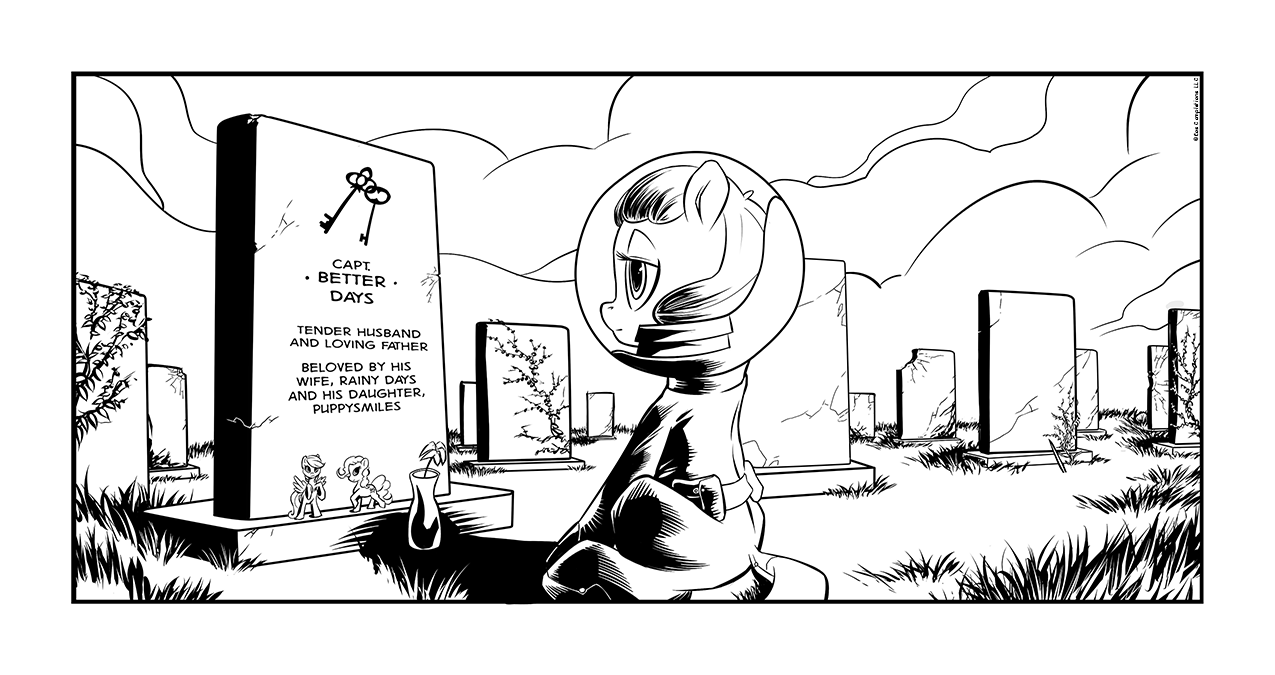
\includegraphics[width=0.9\linewidth]{image16.png}

\begin{intro}
    一个兄弟也不能落下
\end{intro}

「{\rt 我勒个去,伙计们,我简直不敢相信他真的去了!那个羽毛脑袋拿这那个他称之为『步枪』的垃圾烧火棍就那么飞走了!孤狼你如果能听到这个的话,请用那把枪插爆你自己的菊花好么?}」

无线电沉默了一会,然后那个雌驹的声音继续怒骂着。

「{\rt 好吧,朋友们,节目还能继续不是吗?DJ好货现在为您播报52电台。至少在我累趴下之前,因为某个傻蛋把我留下来独自应付一个24小时电台频道!那好,这是我的新规矩,白天我正常广播,晚上只有音乐,因为我又不是什么不老不死不用睡觉的超自然怪物!我也是要吃喝拉撒睡的!如果谁想在晚上找我的话,敲门就是。}」

接下来是一阵翻动纸张的声音。

「{\rt 好吧,不管怎么说,我还是能独自操作这个广播电台的,所以继续把你们的新闻送来就是了,尤其是铁砧镇那边的新闻。说到新闻,纪念碑镇已经被完全摧毁,那里的居民都穿过花椰菜镇到北边避难去了。因此所有要去翡翠海岸的车队,请立刻向北去铁锈庄园,重复一遍,立刻向北去铁锈庄园,不要去花椰菜镇,那里现在太危险了。}」

「{\rt 老娘恨死新闻了,如果有什么消息我会通知你们,如果广播还是音乐那就说明没啥鸟事,这年头没有新闻就是好事。顺便,如果谁见到L.P.请帮我给他脸上来一蹄子。}」


\begin{music}
    小家伙,静静祈祷
    
\begin{englishlyric}
    Say your prayers, little one,
\end{englishlyric}
    
    \medskip

    不要忘记我的孩子
    
\begin{englishlyric}
    Don't forget, my son,
\end{englishlyric}
    
    \medskip

    以及所有小马
    
\begin{englishlyric}
    To include every pone.
\end{englishlyric}
    
    \medskip

    用温暖的怀抱将你包围
    
\begin{englishlyric}
    Tuck you in, warm within,
\end{englishlyric}
    
    \medskip

    洗清所有罪恶
    
\begin{englishlyric}
    Keep you free from sin,
\end{englishlyric}
    
    \medskip

    直到静谧来临。

\begin{englishlyric}
    'til the sandmare she comes
\end{englishlyric}
\end{music}

\horizonline

\daytimeplace{13}{4:00 AM}{民族英雄纪念碑公园,52号国道南段}{The Memorial northern picnic area, Big 52 S Branch}

在帕比的远处是一个小小的居民点,是在一尊巨大的雕塑周围堆起来的一堆破烂窝棚。那个雕塑的内容是几位小马士兵共同举着一面小马国旗帜,巨大的雕塑在很远的地方都可以看得清清楚楚。

在来的路上小雌驹见到了好几个难民车队,用马车载着他们不多的家当匆匆向北逃难,她本来想和那些小马聊天,不过那些小马都忽略了帕比,只有几个小孩子挥着蹄子和帕比打招呼。似乎这里的所有小马都在逃亡,放弃了他们赖以生存的土地和家园。

小雌驹现在站在山丘上,一脸疑惑。「呃,声音先生?我们是不是到了爸爸的地方了?」

「{\mt 分析中,定位当前位置:小马国战争英雄纪念碑公园。您的雄性亲属位置:未知。}」

帕比歪着头四处张望,「对哦,我记得这个地方!那个有萍琪派脸的大大路标!」幼驹撒开蹄子飞奔到路边,越过一堆小土丘之后,看到枯黄的草地上到处都是遗弃的营地和生锈的烤肉架。

「这里就是爸爸在的地方!爸爸就在附近!走吧!」

黄色小雌驹飞快地奔向远处,穿过那些低矮的小土丘。即使走了这么远,战争英雄纪念碑白色的碑体依然依稀可见。

穿过这些山丘之后,帕比看到了一棵死掉的树。在记忆中这里曾经是一棵巨大的橡树,但是现在这里只剩下了烧焦的黑色树枝。

这里曾经也是绿树成荫,翠鸟在碧蓝的天空下歌唱……

\rcpr{「我还要吃苹果派!」}

\rcpr{「别吃那么多帕比,我们还要去爸爸那里,记得吗,如果你吃得太多又会觉得困了,你不想迷迷糊糊地见爸爸,对吧?」}

\rcpr{「妈,他一次都没来过,我们去了很多次他都不在!这一次他会在么?」}

\rcpr{「我……我不知道帕比,不过你可以把漂亮的花留给他呀,他看到的时候会记得你爱着他的,好吗?」}

\rcpr{一对小雄驹相互追逐着消失在山丘之后,这里的小马都在开心玩耍,吃着午餐,大家都很快乐。}

\rcpr{「这一次我有更好的东西!你看!」}

\rcpr{「帕比,这个是你的玩具呀……你真的要把玩具留下么?」}

\rcpr{「当然!这样爸爸回来的时候就能玩到玩具,他就不会觉得寂寞了!而且,他回家的时候也会帮我把玩具带回来吧。」}

\rcpr{「……」}

% NOTE: 漏一句,已补上

\rcpr{母女俩在其他小孩子的欢笑声中沉默着。}

\rcpr{「妈妈?你为什么哭了?」}

绕着这棵巨大的树,小雌驹回忆着之前的时光。她清楚记得春天的时候还在这里野餐。但是现在为什么……大家都去哪里了?记得妈妈说树在冬天叶子会掉光,草也会枯黄,可能现在就是冬天了吧!

小雌驹想着,向记忆之中的地点飞奔过去。

\horizonline

\daytimeplace{13}{6:00 AM}{小马国52烈士陵园,52号国道南段}{Interequestrian 52 War Cemetery, Big 52 S Branch}

这里的墓穴看起来都一模一样,小小的大理石碑上刻着不同的名字,日期,还有一个可爱标记和一段小字。有些石碑是白色,有些是黑色。帕比问妈妈为什么他们颜色不一样的时候,妈妈却叫她安静,不要打搅那些小马的安眠。帕比不喜欢这个回答,因为爸爸是个非常重要的小马,但是却只有一块小小的白色石头。所以她想要带来更多的漂漂花,因为爸爸是最棒的爸爸。

「{\mt 警告,收到求救广播信号,距离:200米,信号辨识完毕:设备009。警告,收到新求救广播信号,距离:200米,信号辨识完毕:设备020。}」

帕比疑惑地歪着头,「啥,新的广播?我希望这一次不是那个一直有小马在喊『救救我们,我们要完蛋了』啥的逗逼信号……」

「{\mt 否定。信号源为和平部 MK VI 防护服。警告,收到新求救广播信号,距离:200米,信号辨识完毕:设备013。}」

雌驹叹了口气:「不是音乐就别烦我啦,我要去看爸爸,或许他已经回来了我们就可以一起去找妈妈了!」帕比说着走向有天角兽雕塑的山坡。

山顶上被矮栅栏包围的是一个烈士公墓,帕比穿过的入口处还有一座高大的坦克雕塑,黄铜牌子上铭记着这里埋葬着的第三装甲师的阵亡官兵。还有一些字写着:因为动力装甲的原因,所以坦克已经不那么常见了。

黄色的小雌驹来过这里可不止一次,所以她对这里的路很熟悉。但是看到这里已经完全沦为一片废墟之后,帕比叹了口气,坐在了一块白色石头前面。

在大理石的表面铭刻着一个可爱标记,还有这么几行字:

% NOTE: 墓碑样式修改

\begin{center}
    队长 \ 晴空·戴斯

    体贴的丈夫\ 和\ 温柔的父亲

    \medskip

    爱妻 \ 阴雨 

    女儿 \ 快乐帕比   
    
    敬上
\end{center}

下面的日期已经模糊不清了,不过对于帕比来说没什么意义,因为她早已经来过这里多次。在这块小小的墓碑前,放着一个空瓶子和几个小玩偶。那个瓶子曾经装着鲜花,不过现在里面只剩下了泥水,那些小玩偶依然站在墓碑上看着帕比,两个发霉的小马玩具其中之一是萍琪派,另一个是云宝黛西。

帕比叹了口气:「他从来没回来拿走礼物,为什么他从来不拿我放在这里的东西呢?我觉得他肯定喜欢萍琪派和云宝黛西的。」小雌驹用蹄子碰了碰蓝色的天马玩具,「爸爸好讨厌哦,要是他能经常回家妈妈也不会那么伤心了……」

不过,妈妈也说过很多次,就算爸爸不回家她也不会生气。小雌驹并不明白为什么,不过每一次说到这些妈妈的眼神似乎都不想再说下去,只是让她听话就好。有一天帕比说爸爸不回家自己也不回家,帕比从来没有见过妈妈那么生气地大哭大叫,后来帕比学会不要去问这个问题,或许某天爸爸想起来还爱着他的妈妈就会回家了。

帕比清了清喉咙,然后说:「拿出所有东西。」

「{\mt 警告,物品管理法术每一次只能拿出一样物品,因此打开快速浏览模式,当你检视完成当前物品时,说『下一个』会拿出下一个物品,说『停止』或者『退出』会结束快速游览模式。}」

一个烟灰缸出现在帕比面前,「下一个!」于是另一个烟灰缸\footnote{烟灰缸(Ashtray):按名称排序,字母A在最靠前的位置}出现了,「下一个!」咻,烟灰缸,「下一个!」烟灰缸,「下一个!」还是烟灰缸……是不是之前提过帕比总是要捡起每一个闪闪发光的东西么?看起来这回要花不少时间。

\horizonline

\daytimeplace{13}{7:00 AM}{小马国52烈士陵园,52号国道南段}{Interequestrian 52 War Cemetery, Big 52 S Branch}

「下一个!」第二十个餐叉收回了帕比包裹里面,然后还滴着水的毛球出现在幼驹面前,「下一……天啊!毛球!」帕比抱起了死去的肉食灵,这个可怜的生物已经没有腿了,只剩下一片翅膀,绿色的粘液从破碎的壳里面流出来,看起来就像是一滩恶心的腐烂物。

「你看起来不是很健康哦,毛球,到底怎么了?」帕比研究着那个死去的生物,想要知道究竟发生了什么,「呃,声音先生,毛球生病了吗?」

「{\mt 否定,毛球已经死亡,并且正在腐烂。}」

帕比皱了皱眉头,她还不太理解那些话的含义,「呃……你是说,她很累么?」

「{\mt 否定,该生物正在变成碎片,正在被自然降解。}」

「什么?」小雌驹警觉地竖起耳朵,「变成碎片?但是毛球不能变成碎片!」她看了看那个尸体,「而且,在我看来好像它还是一整片。」

「{\mt 建议:仔细观察,该生物已经失去三个翅膀和所有的腿,而且因为不良储藏手段正在快速腐烂。}」

「储藏?你是说毛球因为我带着它而变糟么?但是……这太可怕了!」

于是这个没什么自主思考能力的自律智能也劝起了帕比。

「{\mt 肯定,尸体因为你坚持带着它而加快了腐烂进程,推荐您立刻抛弃尸体。}」

帕比很忧伤,「把毛球……留在这里?但是……但是它会寂寞的!这里什么都没有,这里只有……」小雌驹顿了顿,回头看着她父亲的坟墓,「呃……或许爸爸会照顾好它。」小雌驹看起来对这个建议不太感兴趣,虽然看起来这么做没错。

「{\mt 计算,将死亡宠物留给死亡监护人是……错误……错误……请重新思考。}」

「重新啥?你在说什么呢,笨声音,能认真点么。」

「{\mt 再计算,无法找到逻辑,强烈建议寻求其它建议。}」

帕比生气的叫起来:「别说奇怪的话好么,要不然找其他小马来帮我的忙!」小雌驹蹄子按着自己的头盔说:「我说,有时候和你呆在一起真麻烦。」

守望者的金属声音打断了小马和自律智能的争吵,「帕比,你在这里干什么,这里很危险。」

帕比转向声音的方向,黄色的小雌驹看到一个机器精灵飘在那边,不过这一次她没有笑起来,「哦,是你啊,提问者,」

「守望者……」

「随便啦,现在我很烦,回头在找我好么?」

声音迟疑了一下回答道:「可以,但是我现在想警告你,这里不是什么好地方,到处都是……呃……坏蛋,在我走之前你保证赶紧离开这里好么?」

帕比沮丧地哼了一声:「不行,我的毛球生病了,而且声音先生又在发神经!」帕比说着把死掉的肉食灵给机械精灵看。

「哎呦!这东西已经烂掉了!这是啥啊帕比,赶紧扔掉呀!」

「什么?不行!毛球是我最好的宠物和朋友!我喜欢它,它也喜欢我,我们一起冒险这么久了!我不想抛弃它……」幼驹说着撇开了视线,「不过……」

「不过?」守望者追问着,因为帕比抱着尸体不想把话说完。

「不过它病得很重,声音先生说它需要休息……我可以把它放在我爸爸这里,不过好像不太对……因为我还没问他我能不能养宠物……」

「你爸爸?你都知道你爸爸在哪里你还独自在废土上乱逛?」机器的声音听起来有点生气,「到底是哪个不负责任的父亲把自己的孩子……」说到这里,守望者停下了,因为他看到了帕比面前的那块小小石碑。「哦,我的天……还真是……」

幼驹继续说着:「我知道爸爸妈妈说可以,我才能收养宠物……但是……但是……」小雌驹低声哭着,「但是我只是想要个能陪我在一起的朋友!不是一个一直发神经的奇怪声音或者一个来来去去的傻瓜小鸡!毛球从来没有丢下我,一直和我在一起,我们一起玩得很开心,我保护它不被吃宠物妖怪吃掉,而且它从来没有离开过我……」

小雌驹顿了顿,看着机械精灵说:「……现在它生病了,而且腐烂了!声音先生说它之前有更多的翅膀,不过我不太擅长数数,所以我觉得好像他说的没错……我不想把它留在这里,但是我也不想让它因为我而生病……我……我不知道怎么办!」

「啊,那声音先生说什么?」

帕比抹着眼泪,「什么也没说!就是啰里吧嗦的发神经!我想过把它留给爸爸,但是我不知道爸爸是不是喜欢它,爸爸会不会生气……而且,我不知道爸爸什么时候回来这里,因为他从来没有来过这里。虽然妈妈说他爱着我,但是我不知道为什么爸爸一直不见我!」幼驹挥着蹄子,「所以,或许他不会喜欢毛球,毛球也不会开心,但是我不能带着它因为它会腐烂,我觉得腐烂不好……」

守望者纠结着,帕比这番话的沉重感令他一时间不知如何是好。「好吧……或许你可以把毛球给我?把它放在这个机器精灵的货仓里面我来帮你忙?如何?」

帕比歪着头:「你会治好它吗?真的吗!」

「当然,反正它也不会更糟糕了,我看看我能做点什么,不过现在请务必离开这里,这里很危险。」说着,机器精灵旁边打开一个舱门,正好有个可以放肉食灵的空间。

小雌驹看了看这个金属盒子,然后看了看毛球,叹了口气,最后一次抱紧她的宠物,和它低声道别:「别怕,提问者是个漂漂马,等它治好你我们就又可以一起玩了……」在玻璃头盔后面吻别毛球之后,帕比把肉食灵尸体放进机械精灵里面,然后那个舱门关了起来。

「小家伙,别担心她了,她已经去了安全的地方了……现在我们也去安全的地方,好不好?」

小雌驹点了点头,再看了她父亲的坟墓一眼,「百合!」一朵塑料花出现在她面前,她把花朵放在大理石墓碑前,「对不起爸爸,我要走了,下一次我会多等你一会儿,好吗?我会带着妈妈来。」帕比离开了坟墓,转过头面对机器精灵的时候已经带上了她天真的笑容:「好了,我们走!」

「你真是个好孩子,帕比。」

幼驹和机器一起离开烈士陵园,走向纪念碑,那个纪念碑上的小马在常年风化之下已经倒在了地下,正如这里埋葬的士兵一样——在一场没有赢家的愚蠢战争中倒下。

\horizonline

\daytimeplace{13}{7:15 AM}{民族英雄纪念碑,52号国道南段}{The Memorial, Big 52 S Branch}

纪念碑镇已经完全搬空了,这里的居民把所有能带走的都带走了,甚至连松掉的螺栓都拧下来带走了。两个小马骑着狮鹫降落在这里的时候,迎接他们的只有锈迹和灰尘。

「我们到了。」白先生从狮鹫背上跳下来,活动着僵硬的四条腿。「这一路可真远啊。」白苹果的头头扶正他的帽子说:「你们现在可以回太阳城了。」

狮鹫佣兵点了点头,「遵命老大,不过你真的要我们回去吗?」

公马笑了笑,看着身边的另一位小马然后说:「当然,这是家务事,我们只是要你们送我过来,现在没你们的事了。」

看着狮鹫依然不放心的表情,独角兽补充道:「别担心你的酬劳,就算我回不去了,我儿子也会接手公司的。」

带翅的半狮子对其他同伴挥了挥爪子,「好了,你们这群懒翅膀都听到了,走了走了!」于是这些狮鹫都向北边飞去了。

白先生看着那些狮鹫飞走的时候,士官灌木正在把一个沉重的箱子拖进一个用路标之类废铁搭成的小窝棚里面,累得气喘如牛,他抱怨着,「这玩意儿太沉了,白叔叔,你确定我们要拖着这东西走吗?」

「别担心小子,我们就在这里扎营,然后轻装上阵,她不会跑太远。」

「我还是不明白为啥你要自个儿跑这么远,我们大可以叫一大队人马……」

「首先,我们需要尽快来到这里,我们没有那么多空中部队运送士兵和重装备。而且,铁锈庄园出了大价钱雇我们的佣兵队,有钱为啥不去赚。另外,我们又不是来战野牛帮的,我们只是跑过来接小孩的。」

灌木叹了口气,「难道没有人和你说你是个怪胎么,我知道她把我们从火坑里面拉出来的,但是你已经给她报酬了,不管怎么说我觉得这个任务纯属自杀。」公马犹豫了一下,然后又问:「或许还有啥内情?」

白苹果的头头正拿着一个望远镜看着附近的山头,「根据我之前打探的消息,不管那幼驹跑哪儿去,似乎哪里都会变得……嗯……更好,那个『幽灵』肯定是某种福星啥的,我这次要亲眼看看那小雌驹有多大能耐……」

灌木不相信地摆了摆蹄子,「你下这个结论是基于……」

「直觉。」

狙击手以蹄覆面,「我们大老远跑过来找个幽灵是因为你的一个第六感么,为啥我要跟你来?」

白先生笑了,「因为我是你叔叔,而且你欠了我一屁股债。」

「我恨我自己……」灌木刨着地。

白色的独角兽举起蹄子示意安静,「安静,有谁来了,拿枪。」

从他们的狙击地点,两个小马可以清楚看到有谁正在走向小镇,那个旅者满身尘土,厚实的纱巾挡住了她的脸,遮住了她的容貌,在脖子上挂着一长串羽毛和各种小物件装饰的项链。

灌木放下了步枪松了口气,「哎,就是个先知……而已,萨满跑到离沙漠这么远的地方做什么?」

白先生放下枪走出窝棚,「我们马上就知道了。」独角兽说着奔向那个新来的小马。

「喂,叫你呢!这里什么都没有,路南边很危险,你赶紧回去吧。」

戴面纱的小马站住了看着白先生,然后脱下了自己的头纱,露出一个老独角兽雌驹的脸,「你们已经来了……非常好,我们在这里等待其他小马到来吧。」

\horizonline

\daytimeplace{13}{7:30 AM}{纪念碑镇外,52号国道南段}{The Memorial outskirts, Big 52 S Branch}

「对了帕比,你还没跟我说过你鬃毛里面的蓝条是怎么回事,怎么来的?」机器精灵漂浮在帕比身边,他们俩慢慢地走向纪念碑镇,烈士陵园的大门就在他们身后。

「啊,就是在太阳城,蓝音欺负我的时候,我记得不太清楚,不过好像是我睡着了,醒来以后我的鬃毛就变得这么时髦了。」

「这样啊……你睡着了再醒来鬃毛就变了?蓝先生和你说啥了?」

帕比叹了口气,「我和你说过了呀,他说我是个机器马,不过我好好教训了他,而且那都是过去的事了,现在我们已经是好朋友了。」

「啥啥啥?你们是朋友?你不是用一个魔能脉冲弹头炸死他了么。」

帕比咯咯笑着,「当然不是,笨笨提问者,他不是坏机器,不过是一个傻瓜男生!第二次见面的时候怕音帮我教训了他,他和我道歉了,虽然他嘴巴有点毒不过我还是把他当做好朋友!」

「怕什么?」守望者的声音听起来有些担心了。

帕比戳了戳头盔,「你知道的,怕音,住在我脑袋里面说奇怪事情但是又酷酷的坏女孩。」

在一阵长长的沉默之后,机器精灵问:「你是说声音先生么?」

「当然不是,声音先生有点无聊而且说些不明觉厉的话,但是怕音不一样,虽然有点可怕但是酷酷的,她超级厉害的,可以砸烂铁门打飞坏机器。」

机器的喇叭里传来一声惊叹:「哦!我懂了,是你的想象朋友是么?」

帕比歪着头,有点疑惑的说:「她看起来不那么香香?不过好像也没错……」

「好孩子,你总是……」

轰隆!

守望者就在帕比面前消失在一团火球之中。

小雌驹后退了几步,想要搞清楚发生了什么事情。然后她注意到远处有一个巨大的金属物体正在缓缓向她驶来,她马上就明白那是什么了。

「哼,坏机器……」

\horizonline

\daytimeplace{13}{8:00 AM}{民族英雄纪念碑,52号国道南段}{The Memorial, Big 52 S Branch}

白先生坐在窝棚里面的一张桌子后面,而灌木正在一边煮着燕麦。

「长耳,你说的那些小马什么时候会来?」

雌驹耸了耸肩,目视着窗外远处灰暗的天空,「我们明天晚上之前要出发,将会有很多小马,很多腥风血雨……」

灌木转向先知:「老巫婆,我们不是来打仗的,我们只是来接那个幼驹回闹市区,我才不管你那什么疯狂的『预言』。」

白先生对他侄子挥了挥蹄子示意他安静,「你做你的饭,我负责交谈,我想我们早就说好了。」然后他继续问着那母马:「那么,你看到了什么?」

长耳闭上了眼睛,「在梦中我看到火焰从南方燃起,吞没了沿途所有小镇,在熊熊烈焰之中一个粉色的身影在挣扎着,火焰在她穿过的时候似乎熄灭了一些,但是在她离开之后,火焰继续向北边肆虐,而那个身影则在道路的尽头变为黑暗。」

白先生皱起了眉头,「变成黑暗?那是什么意思?」

「一个黑色的波纹在火焰之后形成,并且摧毁了所有东西。」母马叹了口气,当黑色的波纹熄灭火焰之后,整条道路都归于虚无,成为废弃的荒野。」

「好吧,正如我之前的不详预感一样,」灌木叫了起来,「我们赶紧收拾东西回闹市区吧!」

白色独角兽叹了口气,不管他的侄子继续问道:「那么,我们来这里能做什么?」

长耳的视线从窗外回到独角兽身上。「为了阻止火焰毁灭一切,然后在粉色幽影到达道路尽头之前阻止她。」

「粉色幽影?你说啥,我好像觉得你是不是在说那个孤狼说的小小幽灵?」

忽然一声巨响打断了白先生的话,他看着窗外却看不到任何爆炸。

「是火炮?」

爆炸声听起来有点距离,大概在几公里之外。不过白苹果的老大走到外面的时候,却没有任何声音了,不过不知道是不是幻觉,另一只小马出现在远处,身穿一件破烂的披风,头上还带着一顶大帽子。

独角兽喊了起来:「喂,你!这里很危险,回花椰菜镇去!」不过在看清楚来者之后,白先生的声音变了。

「你这个老木乃伊……」

融金微笑着走进白先生,「什么风把你吹这里来了老白,我觉得我最不可能在这里碰见的就是你了,你在这个前哨站做什么?这里有做生意的对象?」

独角兽皱起眉头,「老家伙,我可没打算抢你的工作,我们只是在……侦察野牛帮的动向。」他说到这里顿了一下,观察着尸鬼的表情,「那么你在这战火纷飞的地方做啥,这里有珍宝么?」

百年老尸哼了一声,用嘶哑的声音说:「差不多,应该说我不小心送走一个危险物品,所以我打算弥补之前的过错。」

「从来没听过你这个老混蛋还有吃后悔药的时候,怎么了?年纪大了?」

让白先生惊奇的是,老木乃伊没有反驳,只是看着南方。「你说的没错,平时我可不会关心一个幼驹的死活,现在我却去要救一个小鬼。」

白先生的表情慢慢地从惊讶变为微笑。「欢迎加入俱乐部,进来吧,里面不但有燕麦还有美女。」

\horizonline

\daytimeplace{13}{7:45 AM}{民族英雄纪念碑南广场,52号国道南段}{The Memorial southern picnic area, Big 52 S Branch}

帕比冲向那个巨大的机器,而发光的「命运之石」就漂浮在她身边,「你这个坏机器,不准欺负我朋友!」

而帕比冲向的目标,则是一辆锈迹斑斑的老式坦克,不过即使有接近三个世纪的寿命,这辆坦克依然状态良好,一只有刺猬一样鬃毛的小马正坐在车长的位置看着冲向他们的小雌驹。

「肏他妈的命令,为啥我们要在这里蹲着,我们有坦克好不好,坦克!有这宝贝儿我们可以碾平那些原始马。」

「灰质,那黄色东西正朝我们跑过来,不如来点移动靶射击练习?」那个舱口的小马大笑着,回到坦克里面关上舱门。坦克的炮塔开始转向正在跑过来的小马。

在坦克中,那个刺头正疯狂的笑着,「来啊小家伙!」

「等等!」一个剃光头的雌驹用蹄子戳了炮手的屁股,「我们玩点别的!我要玩玩这个!」

「闭嘴,傻……」那个公马正准备把那个多管闲事的雌驹骂个狗血淋头,但是却看到了她蹄子指着的那个红色按钮。「对哦!我也想试试看,让我们用火箭把它炸到月亮上去!」

「你们俩傻逼能不能少说话多开炮?」陆马驾驶员发火了。

炮手笑着:「伙计,你真是个暴脾气,灰质,看这个!」

这个时候,帕比刚刚跑了一半,她可以清楚地看到那个坏机器有一个方方正正的身体,还有个圆脑袋和长长长长的鼻子……想起来了!这个不是坏机器,是马车!是那些有大茶壶的车子!

小雌驹停了下来,好吧……这东西应该不是坏机器,因为车子一般都会有小马在上面,不过她现在看不到上面有小马,而且它还打坏了提问者的机器,这绝对是坏机器干的事情,所以帕比有点不确定这东西到底是坏机器还是车子,她在考虑是不是要去问问看。

这个时候,坦克炮塔上飞出一道白烟,一发火箭弹射了出来,朝帕比飞去,看起来就像个可笑的大号烟花。

「呦呵!好厉害!烟火耶!」

轰隆!

火箭弹打中了小雌驹身后,把小雌驹炸飞了出去,然后一个倒栽葱摔倒在坦克面前。帕比的头盔都碎了,防护服上也都是破洞。粉红色的迷雾从防护服上的破洞喷出来,环绕在帕比身边。

「好吧,这绝对是坏机器……」帕比慢慢站起身,瞪着在她面前的那个巨大钢铁怪物。在粉红色的迷雾之中,没有头盔的帕比面容已经模糊不清,只有两只发着粉色光芒的双眸清晰可辨。

「黄色的玩意儿,尝尝这个!」刺头狂笑着,但是那个雌驹又戳了他一下。

「又怎么了臭婊子?」

「喂,我说,那东西又站起来了……」

「怎么回事?灰质,碾碎它!」

不管怎么说,废土上很多奇妙的东西,当然也包括被火箭弹上脸还能活蹦乱跳的东西,不过那些强盗觉得被坦克的履带碾过绝对能搞定一切。

于是坦克开始缓缓向前,对准小雌驹开了过去,不过帕比也同样冲向坦克,并且在两条履带碰到她之间敏捷的蹦了起来,用蹄子抓着前装甲板跳上了炮塔。

「那东西上坦克了!好运姐,出去打爆它!」驾驶员忽然一个急刹车想把那东西甩下去,可惜帕比抓得紧紧的,而炮手却猝不及防一头撞上瞄准仪昏了过去。

「别担心,看我的!」雌驹用魔法飘着一把冲锋枪打开舱门,发现在她面前就是被一团粉云包围着的小雌驹。「拜拜,怪物!」

帕比听到面前好像传来有谁说话的声音,但是她转过头只看到个小马形状的东西,但是马上就挨了一梭子子弹,打碎了刚刚自动维修好的头盔。

「坏机器,别闹了!」

帕比这一次真的生气了,她跳到了坦克顶上,但是坦克的舱门立刻紧紧关上了。

「你觉得你能把我关在外面吗?我可是快乐帕比,我想去哪儿就去哪儿!」

幼驹举起石头,在炮塔上寻找着可以砸烂的东西,不过都是各种铁块,哦,一个玻璃镜子,……咣当……铁块,铁块,哦,天线,……叮……叮……叮……,还有一个大盒子?「好了,坏机器,打屁股时间到了!」帕比很喜欢怕音说的这句话,听起来坏得有范儿!

而在坦克里面,好运姐正在因为吸入粉雾而大口吐血,额头上肿着大包的炮手还没有醒过来,而驾驶员灰质正在在蹄忙嘴乱的衔着一瓶治疗药水喂给重伤的雌驹。大家都忙得不可开交,而没有注意到那个幼驹正在坦克顶上用石头敲着坦克的火箭发射器。

这差不多是白先生听到那声巨响的时间。

\horizonline

\daytimeplace{13}{9:00 AM}{小马国烈士陵园,52号国道南段}{Interequestrian 52 War Cemetery, Big 52 S Branch}

三个小小的身影在坟墓之间沉默地站了起来。它们全穿着 MK VI 防护服,就像帕比那件,不过里面不是幼驹,而是腐烂到皮包骨的僵尸。在它们黑洞洞的眼眶之中看不出一丝智慧的光芒,只燃烧着一团粉色的火焰。它们慢慢地跟着地面上小小的蹄印,就像是追随着猎物的猎犬一样,慢慢地向南方走去。


~\vfill

\begin{note}
    升级(Lv 15)

    新技能解锁:卧倒!——怎么回事,我绝对打中她了!

    你对爆炸伤害的抗性提高25点,你可以开心地玩火箭跳了。
\end{note}



\chapter{因缘}

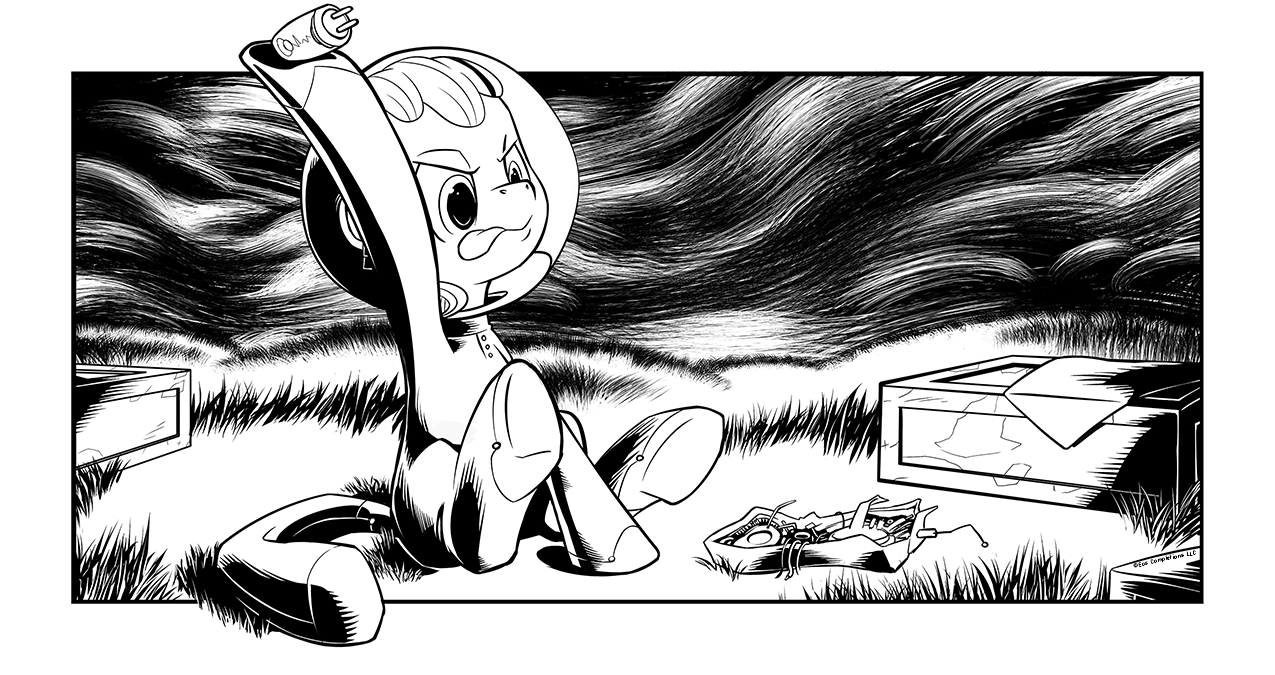
\includegraphics[width=0.9\linewidth]{image17.png}

\begin{intro}
    整个世界都在问这个问题:
    
    {\heiti 谁才是坏蛋?}
\end{intro}

\daytimeplace{13}{6:45 PM}{纪念碑镇北部,52号国道南段}{The Memorial northern picnic area, Big 52 S Branch}

一个雌驹和一个公马顺着52国道南下,他们都背着突击步枪,雌驹穿着保安的防弹衣,而她的伙伴则穿着一身由各种金属板焊在一起的奇怪铠甲,看起来就像是某种廉价喜剧里面的外星马一样。

% FIXME: 译文错误

「我们到底是为了啥离开隧道镇,明明糖霜山的要塞易守难……嗷!」

快乐扳机照坏枪的脑门上就是一蹄子,「我们蹲在要塞,然后看着野牛帮在52国道六成的领土上肆虐么!你怎么是这么一个自私的傻蛋!」

公马撇开视线,「我才不自私……我只是……担心你而已。我不想让你像这样冒险。」雌驹白了他一眼,公马识趣的闭嘴了,不过这也只能让这个热恋中的傻瓜安静半分钟,「至少我们现在先停下过夜吧,纪念碑镇就在附近了。」

「好吧,懒蛋,随你!天啊,你知道你有多烦吗?」快乐扳机咆哮着,「DJ好货已经说了那个镇已经被遗弃了,我觉得那里至少会有比帐篷更好的休息地方。」

说到这里,那座远处倒下的小马国雕像被几个出现的黑影挡住了。

\horizonline

\daytimeplace{13}{7:00 PM}{纪念碑南部公园,52号国道南段}{The Memorial southern picnic area, Big 52 S Branch}

在头盔完全修复之后,一个闪烁的粉色亮点出现在显示屏中央。

「{\mt 系统重启完毕。所有功能正常。自检开始。目标:001号,快乐帕比,雌性陆马幼驹。目标已死亡,体征一切正常。自检完毕。}」

帕比慢慢地睁开眼睛,还是有点昏昏沉沉的。至少从她醒来的地方判断,唉,果然没有从噩梦里面醒来。四周还是枯黄的草和死去的树木,不是她自己的房间。小雌驹叹着气,继续检查粉色箭头的方向,不过某些东西引起了她的注意。

「声音先生,那是啥啊?」

「{\mt 分析中……坦克残骸。威胁等级:无。}」

「不是说那坏机器,傻声音!」帕比叹了口气走到那个东西旁边,「是这个闪光的东西。」

「{\mt 分析中,短波电台,获取加密频道中,新增加通信频道,接到呼叫。}」

「耶!电话!让我接,我要接电话!我超喜欢接电话,拜托了!」帕比清了清嗓子,「嗯哼!您好,漂漂马,妈妈现在不在家!」

一个又惊又怒的雌驹声音从听筒里面传来,「你丫是哪根葱?好运姐在哪?」

耶!是猜谜游戏!「嗨,我是快乐帕比!谁是好运姐?我知道有个小马叫好运气,可以么?」

对方把电话粗暴地挂断了,帕比呆呆地说:「唉,又是恶作剧电话,好吧,别生气,否则正中他们下怀。」帕比耸了耸肩继续前进。

「{\mt 注意:新呼叫,打开通信频道。}」

帕比还没时间回答,和刚才相同的那个声音又出现了。

「听好了混蛋,我觉得这个频道现在不安全了,不过老板现在已经火大了,如果你们丫的不赶紧把坦克开回来那你们就有大麻烦了,懂了么好运,我再说一次,跟灰质那傻叉说叫他麻溜地把坦克开回来,这是老娘最后一次……」

「呦呵,漂漂马又说不明觉厉的话了。」帕比咯咯笑着,作为一个恶作剧电话的话这个蛮有趣的。

「我肏……怎么又是你?肏你妈!」通讯又一次被切断了。

帕比歪着头:「好奇怪哦,或许我们应该赶紧走?」

「{\mt 肯定,主目标地点不在这个方位,注意:新呼叫,打开通信频道。}」

同样的声音再一次说话了,「好运姐,好运姐,这里是小马要塞,请回答。」

帕比笑着回话:「不是,又是我!没关系么?」

那个神秘的声音叹了口气放弃了,「听好,小鬼,我不知道为啥又是你,不过我现在要和某马对话,而你的无线电一直干扰我们的通讯,你到底从哪儿得到这个频道的频率和密码的?」

「什么?密码?我知道!密码是快乐帕比!」小雌驹回答。

「死熊孩子!给老娘关了你的无线电!我正忙着联系一群酒驾坦克手,除非你看过一个坦克在附近晃悠,要不然就别添乱。」

帕比戳着头盔,认真的想着,「坦克?那东西长什么样?」

「你……你有完没完?好吧,那东西很大,有个炮塔有个大炮,还有履带……」声音顿了一下又说:「你见过么?」

帕比看了看就在她旁边冒烟的残骸,然后回答:「呃……那东西是不是还会嘣嘣嘣地把炸弹到处丢?」

「对对对!你见过么?」

「嗯哼,」帕比点了点头,「那是个大坏蛋,所以我用石头把它砸爆了!」

然后一阵长长的沉默之后,对面大发雷霆,「真他妈的,你为啥不找个仙人掌自个儿撞死去?」然后通讯又被切断了。

帕比耸了耸肩,这个新的声音很奇怪,不过帕比应该跟着箭头走,没时间再接恶作剧电话了,不过……她是不是应该对那个恶作剧电话的马来个恶作剧电话?

「呃,声音先生,你能呼叫小马要塞么,超超拜托!」

「{\mt 肯定,打开通讯频道。}」

那个雌性的声音立刻说:「这里是小马要塞,听到请讲!」

「啊……嘻嘻……我是……嘻嘻……咸蛋,请找……嘻嘻……笨蛋先生……嘻嘻……」帕比一边咯咯笑着一边说,她在漫画里面看过这个恶作剧,她自己一直想试试看。

% NOTE: ignore overfull

对面沉默了好久,最后小马要塞回答说:「你丫居然给老娘打恶作剧电话?等我告诉这个笨蛋先生,然后让他把你的屁股打开花。」

帕比大吃一惊:「不要!不要!拜托了,我很抱歉!别……别打我屁股!我会乖乖的!」

一阵大笑之后,那声音回答:「太迟了,恶作剧小鬼!看好你的屁股,因为咸蛋先生和笨蛋先生已经找你去了。」

「咿……呀!」

小雌驹撒开蹄子飞奔向山丘,就好像有无数打屁股板子追在后面一样。快跑吧黄色小鬼,快跑!

\horizonline

\daytimeplace{13}{7:30 PM}{纪念碑镇北部,52号国道南段}{The Memorial northern picnic area, Big 52 S Branch}

别飞得太高,也别飞得太低,老天马,不要一时冲动做傻事……

孤狼飞过重重山丘,寻找着远处可辨的地标,在过了花椰菜镇之后他一直保持低空滑翔,不过随着天色变暗地面上什么都看不清了。

「见鬼,我还是赶紧找个地方过夜,我可不想一头撞上强盗的巡逻队。」天马想着,落在一个小山丘上休息自己的翅膀,「好吧,我到哪了?」

DJ 一直用自己的哔哔小马用低音量播放着52电台,当音乐声停止DJ好货开始说话的时候他放下了地图仔细听着新闻。

「{\rt 好了,小马们,这里是DJ好货为您播报的52电台,不过现在没什么好消息。}」

DJ 叹了口气,听起来马上要哭出来的样子。

「{\rt 铁砧镇已经不复存在了,我前几分钟之前刚刚收到消息,野牛帮已经攻破城镇大门,幸存者撤退回了小镇的避难厩。野牛帮有重武器,战斗机器马,还有更多的东西……现在与一场血腥屠戮只有一道避难厩大门之隔的,是两百只小马,大多数都是妇孺。}」

孤狼叹了口气,摇着头小声说:「孩子,这可帮不上什么忙,在广播里面像个孩子一样哭鼻子不能解决问题,小马需要你的声音领导他们,而不是……」天马叹了口气,「难道每件事都非得我自己来才行?」

「{\rt 很抱歉,大家,我还不习惯做这个……不管怎么说这不是我的错,不过我认为我们还有希望,毕竟幸存者们固守的那扇避难厩大门不是那么容易打开的。所以,你们仔细想想,野牛帮的下一个受害者可能就是你,虽然你现在安全地缩在角落里面,但是你躲得了一时躲不了一世,52号国道是一个整体,如果铁砧今天陷落了,明天将会是花椰菜,然后是铁锈庄园……这样下去野牛帮的肆虐将不可阻挡。}」

孤狼打了一个响鼻收起了翅膀,静静听着那个雌驹的声音,DJ好货的语气也变得越来越自信,好像是她终于找到了她的信念。

「{\rt 但是!如果我们在那之前站在一起面对他们,如果我们能一起去拯救铁砧镇的那些无辜小马,我想我们还有胜算,只需要肩并肩,蹄挨蹄站在一起。孤狼已经去和你们一同战斗,我们只要追随他的脚步!}」

「还不赖,虽然还有很大进步空间,不过至少她没让他们能跑多远跑多远……」天马叹了口气,「至少证明把她留下不是错。」

「{\rt 我想我说得太多了,我们还是继续之前的音乐,这里为铁砧镇献上一曲,请不要轻易放弃,救援马上就到!坚持住小马们!我们只要相互信任,一切都会变好!}」


\begin{music}
    如果只有一匹马相信你
    
\begin{englishlyric}
    If just one pony believes in you,
\end{englishlyric}
    
    \medskip

    他强壮而又有力,深信着你
    
\begin{englishlyric}
    Deep enough and strong enough, believes in you,
\end{englishlyric}
    
    \medskip

    他忠贞而又强大,深爱着你
    
\begin{englishlyric}
    Hard enough and long enough, before you knew it,
\end{englishlyric}
    
    \medskip

    如果有那么一匹马,那么我也可以做到
    
\begin{englishlyric}
    Somepony would think, if he can do it, I can do it,
\end{englishlyric}
    
    \medskip

    我们大家都站在你那边
    
\begin{englishlyric}
    Making it two,
\end{englishlyric}
    
    \medskip

    你绝对不会孤独
    
\begin{englishlyric}
    Two whole ponies believe in you.
\end{englishlyric}
\end{music}

孤狼打了一个响鼻,「还真选了个不错的歌,虽然有点孩子气,不过既然我们是去拯救孩子们,那么我想这样也可以。」小马笑着,走向纪念碑镇。

\horizonline

\daytimeplace{13}{9:00 PM}{废土,52号国道南段}{Wastelands, Big 52 S Branch}

五个强盗现在完全摸不着头脑,因为站在他们面前的黄色幼驹违反了两条废土准则——首先小马们见到他们应该是掉头就跑,而不是跑过来求助。其次小马在连中数枪之后应该死掉,而不是像这个一样活蹦乱跳。

「求求求求求您了!快把我藏起来!他马上就追过来了,拜托,拜托!拜托了!」帕比焦急地来回踏着蹄子。「我已经说我很抱歉了,但是他还是要追我!」

一个脖子上留着一道大伤疤的陆马雄驹走向幼驹,而其他四个则举枪跟在后面,「你丫到底是谁,你丫到底是啥,什么东西能追你?而且为啥肏他妈的你还活着?」那马低头看着帕比胸口上的弹孔现在早已经消失了,而且她一点痛苦的表情都没有。所以说,听这个诡异的小孩把话说完是个好主意。

「呃……我……我是……」帕比愣住了,如果这些马其中之一是笨蛋先生或者咸蛋先生呢?她要放聪明点。「我……我是……啊……幽灵!我绝对是那个收音机里面一直在说的幽灵!而且,我的名字是……呃……不叫快乐帕比。」来回打量这几个小马之后,幼驹又弱弱地追问一句:「这里没有马叫笨蛋或者咸蛋吧?」

公马慢慢地点了点头,粉色的闪光双眸,黄色的防辐射服,不怕子弹……没错,就和那个传说中的幽灵一样,「所以……你就是52号国道的幽灵?」

「没错!」帕比点点头,现在她的说谎技巧就面临考验了。帕比,你要聪明点,露出不在乎的表情!

「你的名字是……『不叫快乐帕比』?」

「对对对!」看起来有效了!他们上当了!欢呼吧帕比,你是说谎话大师!

「那个52号国道的幽灵?那个拯救城市的机器马杀手?」除了第一位小马之外,其他几个都吓得退了一步。

「就是我!」帕比用力点着头。

「你想要我们的帮助?」公马有点迷糊了。

「没错!呃……如果说你们没有马叫笨蛋先生的话。」

「我……好吧,我叫砍刀,那个独角兽是伤管,他的娘们儿是切纸。然后那俩是臭尾和塑料花。」公马指着剩下的俩雌驹介绍着,除了伤管和切纸,其他两个都是陆马。

帕比松了一口气,「哎呦,真是太悬了,那啥,有个疯子正在追我,因为我给她打了一个恶作剧电话,所以她现在想打我屁股,我……我能……我能和你们混一会儿么?等他来的时候你们可以跟他说我是个好孩子让他不要打我屁股好么?超超拜托!」

砍刀看了看他缩在后面的伙伴,另外一个公马耸了耸肩,其他三个雌驹也一副不想管闲事的表情。「你真的只是因为有马想要打你屁股才跑的?」

小雌驹点点头。

强盗叹了口气,「你傻啊!」

「呃……或许有点?如果我真傻你们可以帮我么?」

公马又叹了口气,他今天叹了好多次气了,「反正你也会跟着我们,是吧?」

帕比笑着点了点头。

\horizonline

\daytimeplace{13}{10:00 PM}{纪念碑镇,52号国道南段}{The Memorial, Big 52 S Branch}

白先生一边把一个铁罐子塞进自己包包,一边冷笑着。「只是因为一个你不认识的小马,你就丢下自己的电台一路飞到这里?」

「差不多……我感觉到起风了,而且……我想要在那事情发生的时候在现场,我很惊讶你们也在这里……」孤狼看着窝棚里面的一群马回答着。

到目前为止,这里有一个来自沙漠里的先知,隧道镇的警长和她的……情夫?男友?都差不多,还有小马国最著名的盗墓者融金,还有这位白苹果家族的白先生和他侄子。

「你们有啥高见?」天马看着夜空等着先知开口。

「我们还在等其他朋友,我们明天再行动,现在野火正旺,我们必须等待火焰即将熄灭的时候再行动。」长耳闭上眼睛深吸一口气说。

「听好了,我才不管你那什么破预言!」快乐扳机打断她:「我只想知道帕比是否安全,你这个嗑药的知道么?」

独角兽雌驹睁开眼睛回答道:「我怎么可能知道,我不可能选择预知梦的内容。」

乐乐懒得理她,转头走向角落的那个尸鬼,融金在她来这里之后一句话也没说,不过他现在看起来心事重重。

「老木乃伊,你经常来北边……」雌驹对宝物猎手微微一笑,虽然不喜欢这个老尸鬼,不过他也没做什么惹雌驹厌恶的事情——至少现在还没。「我很好奇,那个幼驹对你做了什么?」

尸鬼转头看着这位守卫队长,「那个幼驹没有对我做什么……而是因为我没有对她做我该做的事情。」融金一声自嘲地冷笑就像是白骨刮过金属一般,「两个世纪以来,我第一次感觉到内疚,你相信么?」

灌木摇了摇头,现在这里看起来就像是那种「讲自己的故事」然后大家一起「哦,好可怜」叹息的社区集会。「你还是说吧,我觉得这里的大多数都活不下来,所以不必担心你的小秘密被别的马知道。」狙击手轻蔑地哼了一声,然后补充道:「等大家都讲完伤心事之后我们可以来场枕头大战了。」

白先生以蹄覆面,「灌木,你不说话没马当你是哑巴。」

尸鬼开始用他那沙哑的声音讲述自己的故事。

「我正好认识帕比的妈妈,阴雨。她也算是某种英雄,不过并不是那么特别,但是在炸弹刚刚落下来的那些日子里,每匹马都惶惶不可终日。是她组织起难民营,将我们聚集起来,给我们活下去的信念和力量,帮助了很多小马。她教会小马们如何自救,如何保护自己,然后又离开,去下一个城市,做同样的事情,在这片废土上点燃52国道沿途的文明之火。」

坏枪跳了起来,「既然你知道这些,你又和帕比说了什么?」

融金瞪着那个卫兵,低声说:「我能和她说什么?『抱歉你妈妈已经死了?』你有看过她的那双眼睛么?所以我送她去了象牙塔,希望那里的铁骑卫可以找到办法帮助她……」尸鬼顿了一下,然后又转开头补充道,「……安息。」

大家一瞬间都安静了下来,不过这时候快乐扳机叫了起来:「我说,象牙塔完全被毁了,你还送那孩子去那里?」雌驹怒气冲冲地举起枪,「你这个龟儿……」

坏枪和孤狼一起按下了女警卫,「乐乐,冷静,之后还有人在花椰菜看到了她,她没事的!」

融金叹了口气摇着头说:「没错,她肯定不会有事,而且有趣的是,象牙塔的大多数小马都安然无恙……不过是他们的老窝被炸了而已。如果有谁告诉我是那个孩子干的,我倒是一点都不奇怪。」

孤狼放开了快乐扳机,然后站起来说:「有两个被帕比救了的奴隶和我说,她看起来就和幽灵一样,子弹穿过她的身体就像什么也不存在一样,而她发着粉光的眼神催眠那些强盗自相残杀……话说,你们相信幽灵么?」

「我勒个去,」乐乐生气地大叫起来,「蠢蛋,别跟我说这个好么。我家那二货已经在通道镇问过这个问题了,虽然我承认这个幼驹看起来不太寻常,但是我亲自抱过她,我很确信她是真实存在的!」

白先生看着窗外说:「我觉得我们是不是至少有个放哨的,有几个小马从北边来了。」

所有的小马都转向长耳等她开口,先知微笑着站起来走向门口,「他们来的比预期的要早……我们去见见著名的铁骑卫吧。」

\horizonline

\daytimeplace{13}{10:30 PM}{废土,52号国道南段}{Wastelands, Big 52 S Branch}

小小的营火在营地中央跳跃着,两个陆马雌驹在煮着罐头装的食物,其他小马则在擦拭着武器,所有小马都尽量忽略帕比。

臭尾低声和伤管咬着耳朵,「你觉得他们已经打开避难厩了么?」

独角兽耸耸肩,继续擦拭着武器,「早晚的事,那些肥猪让我们饿了这么久,这次要把他们都宰了!」他啐了一口恶狠狠地说:「去年我们饿死了十一个,我现在已经等不及要杀进去让他们血债血偿了。」

塑料花冷笑着补充道:「那些肏蛋货占着所有肥沃田地,把所有好东西都自己独吞了……这次他们都要吐出来。」

砍刀也点了点头,「铁砧镇,铁锈庄园,盐块城,所有这些城市都要烧成灰烬!」

帕比虽然不太懂他们在说什么,不过她觉得他们清理武器的办法太没有效率了,有更好的办法把东西弄干净。「呃,为什么你们只是擦那当当响的东西,为什么不把那东西丢进水里洗,那多方便!」

一路上这个小雌驹绝对是有型的噪音源,无尽的语言折磨,那些强盗骂她也好,用枪打她也好,完全不管用,她就是在吧啦吧啦地说着,只有说要打她屁股还有点用处,不过没有马敢去碰这个完全不怕子弹的东西,而且从她身上弹孔里面漏出来的粉色烟雾看起来很危险,而且更恐怖的是,那些粉色烟雾就像有生命一样。

「这些枪要上油,除非你想它卡壳然后在你嘴里爆炸,」切纸解释道,「你根本不知道什么叫维修保养对吧?」

「维修?我当然会维修!我是最厉害的修理工!」

「修理工?你为啥不先修好自己的脑子。」雌驹笑了起来。

「不,我会修收音机,而且……而且我修了一个大电视!还让我的声音朋友动了起来,他超开心,嗯,我是个声音修理工,大概?」

切纸停下了活看着她,「你……真的会修电子设备?」

这是个好机会!帕比心想,如果让这些小马知道自己有多厉害,那么一定会和他们成为好朋友的!或许笨蛋先生来打她屁股的时候这些朋友可以帮她,或许这些朋友可以帮她找到妈妈!

「当然,我什么都修得好!」

独角兽飘着一个无线电台到帕比面前。「那你证明给我看,这东西下午就坏了,然后我们就和基地联络不上了,如果你能修好它我们就让你加入野牛帮。」

黄色小雌驹看着小无线电咯咯笑着:「上次我修好的那一台有一个屋子那么大呢!小菜一碟!」

咣!咣!咣!

帕比把无线电用力在地上摔着一直到它外壳裂开,然后她看了看里面,一副胸有成竹的样子,「嗯,我知道故障原因了,它坏了!」

独角兽以蹄覆面,正准备拿回比之前还坏得更彻底的无线电时,帕比拦住了她。

「现在我只要把一些闪闪发光的东西塞进去……」帕比拿出一个火花电池塞进可怜的收音机,然后用力敲打了几次,然后在一阵滋滋声中,无线电台恢复工作了。

「什么!你居然修好了?」雌驹一把从幼驹蹄子上抢过无线电,立刻联系基地,「红蟑螂呼叫小马要塞,请回答,重复一遍,红蟑螂呼叫小马要塞,请回答!」

所有小马都屏住呼吸静静的等待着回复。然后这个通信设备新的闪闪电池冒出一阵火花,随之发出一个声音:「这里是小马要塞,红蟑螂你们都去哪儿了?再不回来我们就把你们的东西拍卖了!」

随着这一句话,所有强盗都欢呼起来,兴奋的朝天开枪,帕比也咯咯笑着看着这一幕,砍刀走到她身边拍着她的头盔说:「干得好小家伙!谁知道你居然是个电子天才?我们完全误解你了,欢迎加入野牛帮!」虽然他还想说什么,不过切纸打断了他的话。

「灰质开着坦克不知到哪儿去了,老大想让我们赶紧回铁砧镇。」

塑料花摇着头,「那些傻货开着坦克跑了?我早和老大说过别给那群疯子那玩意,他们从来没想过野牛帮什么事情,他们只是想在52号国道上烧杀抢掠而已。」

「唉,随便了,」臭尾说,「反正我们还有坦克,而且还有机器马,我们这一次绝对不可战胜!」

伤管拍着帕比的背说:「小幽灵,想看看我们的基地么?」

「呃……我不知道……我应该去找我妈妈……她大概在那边……」帕比指着南方。

「那真是太好了!我们也去那边!」砍刀拍着幼驹的头盔,大家都在逗着小帕比玩,而帕比也觉得很开心。

这队强盗的领队说:「好了大伙,拔营,我们连夜赶回铁砧镇!」

\horizonline

\daytimeplace{13}{11:00 PM}{纪念碑镇,52号国道南段}{The Memorial, Big 52 S Branch}

诘责喝着他的茶,看着房间外面的窝棚,「很好,我们现在有个DJ,有个尸鬼,有个投机倒把的,有个瘾君子还有仨民兵?」

老书记官摇了摇头。

「52号国道的最后防线就是你们了?聘蹄的佣兵呢?」

冷浴耸了耸肩,不穿动力装甲的她看起来比一个孩子大不了多少。「随便了,反正我们也没期待它们,我们有自己的部队。」

「这些就是我们阿杰铁卫想要保护的小马么?」

帕拉丁皱着眉头看着诘责,「我可没有看到什么老弱病残,在我看来,他们不过是一群自发组织的民兵队而已,如果他们想参战,我不会阻止他们上前线,不过……」敲门声打断了她的话。

「请进。」

白先生推开门走了进来,「晚上好,书记官诘责和帕拉丁冷浴,」独角兽打量了它们一会然后说,「情况一切正常么?」

诘责打量着他说:「呦,52国道上最有权势的马来了,我可以问一下你,为什么只带了一个士兵来?或者……你们的其他后备队还在路上?」

老白摇了摇头:「不,我现在既不是白苹果的领袖也不是聘蹄的老大,我只是代表自己前来还债的。」

冷浴低声嘟囔着「老吸血鬼还还债」之类的话,不过那公马没有回话。

诘责不管那个交涉能力为负数的同事,继续和白色独角兽说:「还债?我猜猜看,是幽灵的么?」

「你这老家伙比上次见面厉害多了,难道你那长者斗篷还带读心术?好吧,开个玩笑,看起来这里的每一位小马都是被那个小孩子引来的。」

「没错,我很好奇,为什么这样一个灵魂的碎片都能吸引这么多小马,如果说我只是为了遵从阿杰铁卫的誓言那是扯谎,我想亲自跟着那孩子直到她旅途的尽头,」老书记官微微一笑,「不过我想你来这里不是想说那个幽灵的话题的,不是么?」

老白笑了起来,「好吧,的确是这样,关于另一个原因……我毕竟代表了很多小马的利益而来,不管怎么说,我想知道我怎么可以帮助你们铁骑卫赢得下一场战斗。」

「下一场战斗?很有趣,不过我想先问你,你觉得下一场战斗是什么?」

聘蹄的老大打了一个响鼻,「好吧,既然你这么问了,在我看来,你打算在那些强盗还在玩铁砧镇的避难厩大门的时候突袭那些歹徒,在我看来很明显,至少我是打算这么做的。」

老书记官点点头,「没错,很明显,但是我不觉得在花椰菜镇,铁锈庄园和太阳城削弱它们之前我们有机会消灭他们,」诘责回头看着冷浴,「不过这一点你问错马了,战术层面的事情……帕拉丁,你有什么话要说?」

雌驹叹了口气,显然不太喜欢被拖入这场对话,「我不知道野牛帮有什么货,但是如果计划突破敌军防线达到避难厩然后疏散拼命,那么我们的确需要任何可用的协助。」

白先生慢慢点点头,「我听说他们有坦克和战斗机器马,或许我们应该制定一个比径直冲进敌阵被包围集火更好的计划?」

诘责举起蹄子,「不,等等,你理解错了,铁骑卫负责突破防线,你们在外面掩护我们撤退。」

「那还不错,一个不包括我的自杀式进攻么?说实话,我挺喜欢的。」老白一副嘲讽的口气说:「那么如果我们这个『打得他们不知道北』的计划失败呢?」

诘责呲之以鼻,「别担心,我还有B计划,铁骑卫肯定会解决野牛群,就算那需要把天空捅个窟窿。」

\horizonline

\daytimeplace{13}{11:30 PM}{纪念碑镇,52号国道南段}{The Memorial, Big 52 S Branch}

融金坐在外面的一个长椅上,看着远方,嘴中吊着一根点亮的雪茄,他不停地咳嗽着,而快乐扳机默默地坐在了他旁边。

「喂,你见过她妈妈?」雌驹若有所思地问。

「没错。」尸鬼点点头,「我在偷抗辐射药的时候被她抓到了,所以她把我赶出了城,我在辐射地区拾荒的时候用了很多那东西。」

「那么……之后你不吃抗辐射药继续拾荒?」

尸鬼发出他那临死哭号一样的自嘲笑声,「你比看起来聪明多了……那婊子对我干的好事,我永远不会原谅她……不过我也知道那是我活该,不管怎么说,我现在还能跟你说这个故事。」

卫兵迟疑了一下,然后问下一个问题:「那么阴雨女士呢?她……」

融金把香烟丢掉,过了很久才回答:「她不能和你讲这个故事了,我觉得那样更好,大家都喜欢死掉的英雄。」

「但是……但是……但是帕比……等她……」

尸鬼有些恼怒地用蹄子踩灭香烟,「我知道!我第一次见帕比的时候就应该和她说,但是……但是然后呢?」老赏金猎人长叹一口气,「那是那孩子前进的唯一动力……我不知道那幼驹是什么,不过有某种力量让她不可战胜,她有那种决心,那种力量,她让我想起了战前的那些美好时光。」

「战前?」

「对,当我们还坚信塞拉丝蒂亚公主永远不会放弃我们,每一个小马都天性善良,世界都如此翠绿美好的时候,但是我们还不满足,想要得到更多,奢求更多财富……我也不知道为什么。」尸鬼凝视着远方沉浸在自己的回忆之中。「帕比也是那样,她相信每一个小马都天性善良,因为她深信大家都是漂漂马,即使在废土上,这片大地如此腐朽,如此绝望……我……我不想毁掉她的希望。」

卫兵低下了头,「我也是……我……那么,她在这条路的尽头能找到什么呢?」

融金看着南方,低声地说:「一个可以看到翡翠海岸的小山丘上,会有一个刻着名字的小小坟墓……」

快乐扳机完全不知道该说什么。

「那是个安静的地方,你可以听到波涛声,感受海风轻拂你的鬃毛……\ldots 如果你闭上眼睛,就好像又一次回到了小马国的那些光辉岁月。」

「然而,那又有什么用?」雌驹看着自己的蹄子说。

融金叹了口气:「是啊,那又有什么用呢?」

\horizonline

\daytimeplace{14}{5:30 AM}{铁砧镇,52号国道南段}{Ironworks, Big 52 S Branch}

铁砧镇在燃烧。

这里曾经是铁砧城——一个巨大的工业中心,这里曾经耸立着各种宏伟的厂房,里面都是各种机器和忙碌的小马,在炸弹落下来之前,源源不断的钢铁和煤炭运送到这里,被机器加工成各种武器甚至坦克,但是在战争末期这里的工厂大多因为原料短缺而停工,避难厩科技买下了这里的几座工厂,然后在厂房下面建起了避难厩,因为有很多工厂的小马参与了避难厩建设,所以这个避难厩可以说是最先进的几个避难厩之一,并且在炸弹落下的那一天挽救了无数生命。

而在战后,幸存者们在最大的工厂厂房里面建立了一个小镇,整个地方都被建成了要塞,巨大的钢铁城墙上满是各种防守武器。这里一直是52号国道防御外敌的大门,在无数的岁月里面,各种怪物和强盗一次又一次地进攻这里,全部被击退了,因为这里几乎有取之不尽的废金属来修理城墙遭受的一次次攻击。

一直到今天。

在那些吞没大楼的大火中,滚滚黑烟直冲云霄。就在厂房外面是一个临时的营地,无数的帐篷围绕一个个营火立起。帕比和她的新朋友一起走进了这个营地。

「别担心小兄弟,他们绝对不敢惹你,我罩着你呢。」伤管拍着小雌驹的后背鼓励着她,不过看起来完全没有必要,因为帕比正开心地和每一个小马挥着蹄子问好。

「嗨!」幼驹咯咯笑着:「你看那个雌驹,她鬃毛好狂野,哦哦那个可爱标记,超酷!」

一个黄色鬃毛红色毛皮的独角兽走了过来,「你们这些懒鬼还算准时。」

「肏了,要塞……」砍刀转头和帕比说:「她是小马要塞,我们的无线电员……她是个婊子,别听她抱怨,不然你长大也会变成一个婊子。」

帕比不知道那个小马后半句说了什么,所以她开心地蹦跶过去挥着蹄子问好:「嗨,我叫快乐帕比,我正在找我妈妈!」

独角兽忽然愣住了,然后等着小雌驹问:「你刚刚说……快乐帕比?」

「没错!」

帕比点点头。

「你是不是刚好有个无线电?」

幼驹又点点头,自豪地说:「那当然,我超酷的,你是干什么的?」

独角兽用她的魔法把小雌驹抓了起来,蹲在地上把小雌驹放在她面,然后前举起一只蹄子。

「那好,现在我们来算总账。」

小雌驹挣扎着想要逃走,但是她能做的就只有乱挥着蹄子。

「放开我!放开我!!」

「乖孩子!」

啪!

「不可以!」

啪!

「打!」

啪!

「骚扰!」

啪!

「电话!」

啪!

帕比拼命地哭叫着,但是红蟑螂并没有冲过来救她,而且那五个小马还站在那里看着她挨打,一起大笑着。这个不死怪物看起来完全输给了坏脾气的无线电员。不过话又说回来,一个小丫头片子有什么好怕的。

「对不起,对不起,对不起!」帕比像个孩子一样哇哇哭着,但是雌驹完全没有停下来的意思,一边训着她一边打着她的屁股。

等这场风暴结束之后,小马要塞把她放下然后看着她的眼睛怒喝道,「你丫还敢恶作剧么?」

帕比一言不发地拼命摇头。

「看着我,我在和你说话呢!懂了没有?无线电不是玩具!如果你一直占着频道会误大事的,你听懂了没有,嗯?」

等小雌驹被训够之后,切纸走到了小马要塞面前,「别和孩子一般见识了……而且不管怎么说,她修好了我们的无线电,不然我们还在继续我们另外三天的巡逻呢。」切纸拍着帕比的头盔说:「她是个乖孩子,她知道自己做错了,而且也认错了,你们俩可以和好么?」

小马要塞打了一个响鼻:「如果她真的懂了的话,那好。」

「好了好了,来碰个蹄子……帕比现在是我的小弟,你在欺负她就等于欺负我了!」

无线电操作员叹了口气伸出蹄子,「好了好了,反正我也消气了。」

黄色的小雌驹忍着自己的哭声,伸出自己的小蹄子碰了碰独角兽的蹄子。

「好了,我们扯平了,欢迎加入野牛帮。还有你,应该先带她见老大。」

\horizonline

\daytimeplace{14}{5:30 AM}{纪念碑镇,52号国道南段}{The Memorial, Big 52 S Branch}

长耳忽然惊叫一声跳了起来,吓得老白从床上滚了下来。

「怎……怎么了,女巫?」公马一边找他的枪一边问。

先知叹了一口气,遥望着南方。「已经开始了,我们要尽快行动。」

\clearpage

~\vfill

\begin{note}
    升级(Lv 16)

    新专长解锁:黄色冲刺——跑啊!快跑帕比!当你身穿轻甲或者无甲的时候,比如穿 MK VI 全封闭式防辐射服。(还能有啥?)你移动速度提升10\%。别太开心,你依然会被打屁股。

    新剧情专长解锁:入会——你现在是野牛帮的一份子了,你在野牛帮的声望重置为中立。
\end{note}



\chapter{迷雾}

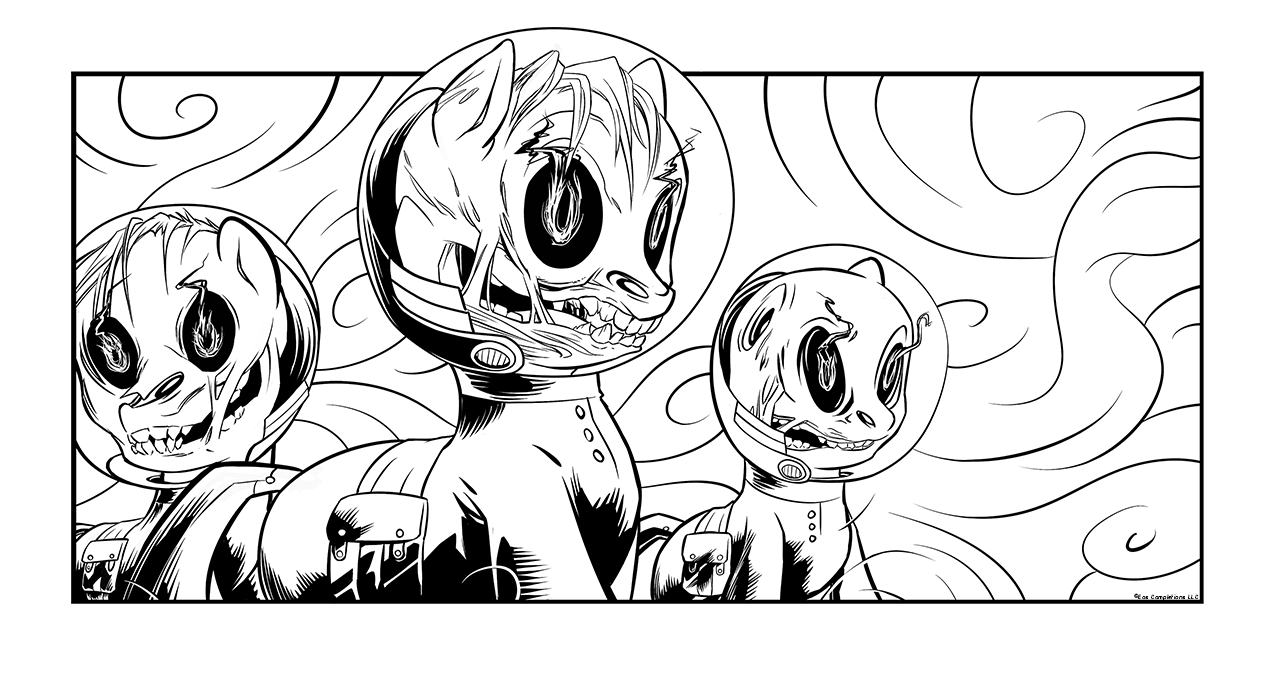
\includegraphics[width=0.9\linewidth]{image18.png}

\begin{intro}
    为熊孩子带来的浩劫而哭泣吧!\footnote{这一句话恶搞莎士比亚的凯撒大帝}
\end{intro}

\daytimeplace{14}{6:00 AM}{纪念碑镇,52号国道南段}{The Memorial, Big 52 S Branch}

「哦咿呦……」

白先生走进窝棚,低头看着长耳坐在一圈小骨头围成的一个圆环之中,她的角上挂着很多发亮的小珠,看起来就像一蘸提灯。雌驹用一个奇怪的姿势坐着,她的后蹄子盘在身体前面,前蹄像绽放的花朵一样打开。她真是……太奇怪了。这个先知居然不是一个斑马。公马对此非常好奇。

在房间的另一边,灌木正在为去铁砧镇而做着最后的准备,白先生的侄子完全不受长耳的影响,仔细地整备着他的武器。

「好吧,她到底在干啥?」白苹果的领袖一脸迷糊地看着那先知。

灌木耸耸肩,「我不清楚,她说她要作法让敌人笼罩在什么『战争迷雾』之中,然后就嗑了一大堆药坐在那里『哦呦哦呦』到现在。」

「嗑药?」白苹果皱了皱眉头,整个屋子里面都是药草燃烧的味道,熏得他晕晕乎乎的。那些气味很奇怪,虽然觉得不对头,不过他也说不上来哪里不对。

「哦呦呵……」

「比如说,曼他特啥的,吃了超级多,还有很多白色的药片和从来没有见过的绿色东西,她把一部分放烟壶里面抽了,然后把剩下的灌肚子里……而且她还喝了不少,你懂的,对于我的酒量而言,不少是多少。」

「然后呢,她就那样神神叨叨的?」

老白觉得自己眼前也开始出现点点了,就像鬼火一样,让他觉得有些朦胧,屋子中间的熏香味道实在太浓,让他觉得眼前的一切就好像是做梦一样。

公马摇了摇头,不,不是做梦,是因为那些药品,那些药品切断独角兽对于现实的感知,让小马能专注于魔力的流动,不过那种东西非常非常容易上瘾,而且有毒。

「你说到什么雾?」

灌木点点头,「没错,她叨叨着什么『战争迷雾』之类的,然后就不说话了。」

白色的独角兽抚摸着自己的下巴思索着。「『战争迷雾』?那是啥,把云丢到敌人脑袋上?」老白一点都不明白。

「马上就知道了。」狙击手已经打包好武器,他看起来完全不受那些烟雾影响,或许是因为他的身体比较强壮。「不过如果她不赶快醒来的话,我们只好把她丢在这里了……我还是挺想念她。」

老独角兽皱起眉头,「你可别低估了她,说不定她还能救你一命!」不管谁都可以看得出来那个独角兽老太太不一般,不过,老白也知道和他侄子说那种事情是浪费时间。

「哦咿呦……」

灌木嗤之以鼻:「怎么救,预言我今天会挨几颗枪子?」

和他解释果然是浪费时间。

「或者说,替你挡一两颗枪子?」老白叹了口气。「我们走吧,这里味道臭死了。」

\horizonline

\daytimeplace{14}{6:30 AM}{铁砧镇,52号国道南段}{Ironworks, Big 52 S Branch}

「这位就是那个传闻中的小幽灵?」有着红色鬃毛的红色独角兽低头看着帕比,「一点都不起眼嘛。」

砍刀讪笑着,「马不可貌相,这小家伙简直不可阻挡,而且还会修理各种电子设备。」不过红色公马看起来完全没什么兴趣。

「随便,你想要个宠物的话,怎么都好。赶紧干活去,要不你拿工具去下面帮那些家伙弄开避难厩大门。」

「小菜一碟。」砍刀走回他的部下面前,「你们也听到了,我们去撬开那核桃然后拿财宝去!」他拍了一下帕比的屁股说:「你也一起下去,小幽灵。」

帕比现在很不开心,因为她刚刚又被训斥又挨了打,虽然打屁股现在一点都不疼,但是她觉得心里非常非常疼。因为平常妈妈虽然也训斥她,有时候也打她屁股。但是如果帕比说她知道错了妈妈马上就会抱着她安慰她。这些小马则只是在一边站着嘲笑她,让她觉得很伤心,也没有谁来抱她告诉她没关系。她觉得她应该表现得很能干很厉害,然后这些小马才会喜欢她,就像她刚刚修好无线电台的时候那样。

小雌驹的思绪被塑料花打断了,

「嘿磨蹭鬼,你来还是不来?」

「当然,我来……」帕比有气无力地回答着,然后小雌驹立刻屁颠屁颠地跟着那几匹马走过去了。

血浴看着这群小马走开,然后低头看着桌子上的地图,视线从铁砧镇的红圈上跳到52国道上一个又一个小镇上。他露出一阵满足的冷笑,探子回报纪念碑镇已经完全被遗弃,那么接下来就变得更简单了。

现在这个强盗头头心中的唯一芥蒂就是来自北边的小麻烦,好运的坦克完全失去联络,而那群红蟑螂饭桶也没找到一丝线索,反而带回一个穿着防辐射服的智障儿。

52号国道的幽灵……如果她真的是英雄的话,看起来也没什么威胁,而且更好的是,她现在已经是野牛帮最烂小队的吉祥物了。52号国道的居民应该选个更好的英雄。

一个飘进来的机械精灵打断了血浴统治52国道的美梦,他非常恼怒的瞪着入侵者。

「又咋了?」

机械精灵闪着蓝光发出旭日系统的声音,「血浴,这样不对,用现有装备切开避难厩大门需要花费大量时间,我强烈建议我们继续北上,否则会给敌人组织防御力量的时间。」

血浴笑了起来,「给他们多少时间也没用了!它们不过是等着被打翻的保龄球瓶而已,我们现在在这里以逸待劳,然后让整条52国道都在我们前进的马蹄下颤抖,然后他们就会在恐惧之中拜倒在我蹄下!他们绝对不会反击,他们只会逃跑。就算子弹可以挡得住,但是没有东西可以挡得住恐惧本身。」

旭日系统看起来对这段煽动演说毫不感冒,「洗脑才更加有效率,根据我的计算,你只是在毫无意义地杀戮行为上浪费大量的资源,或许我需要寻求更佳解决方案了。」

公马恼怒地皱着眉头,走到那个机械精灵面前面对着它。「你这个没用的破烂给我听好了,你给我们武器和机器马,但是你要搞清楚,我才是野牛帮的头头,是我给你分享胜利果实的机会。等我们碾碎了52号国道,我可以给你足够的地方和瓶盖让你买奴隶来重建你的什么太阳帝国。但是这些小马,这条52国道上的所有小马,一个活口都不能留,我可不想给他们翻账的机会!」

旭日系统只是静静地等他扯完长篇大论,然后说:「这违背我们当初的合作协定,如果你继续这种行为,我将会撤离所有战斗机甲,或许我该找个更好的合作伙伴了。」

血浴冷笑一声:「你觉得你可以要挟我?我才不在乎你那没用的铁罐,我现在有足够的坦克和重武器!」公马一蹄子把一个空箱子踏得粉碎。

「那好,再见。」机械精灵说着转头飞走。

「等等,肏蛋货……算你赢了!你去楼下告诉那些撬避难厩大门的小马,让他们只杀掉反抗的,剩下的抓做俘虏。」红色独角兽啐了一口低声说,心想,反正我们之后可以随时处决他们。

机械精灵满意地点了点头,「很好,你还是讲理的,那么回头见。」机器说着飞出了帐篷,飞入浓浓的晨雾之中。

在那机器飞出帐篷之后,另一只小马走了进来,「我说老大,这雾气不停地从山上涌下来,就算不是独角兽,也能看出来有谁在给这里施咒……」

血浴大笑着,「那些孬种,他们觉得这种东西可以掩盖他们的驽弱偷袭?别笑掉我的大牙了。」独角兽狂笑了一阵之后,走出了帐篷开始下命令,「所有带哔哔小马的带队出去巡逻,给他们每匹马一把冲锋枪和曼他特。」

那个部下点点头,「马上去办!」他说着跑出了帐篷。

在迷雾之中,三个黄色的小小身影寻觅着帕比的蹄印,慢慢靠近营地。

\horizonline

\daytimeplace{14}{7:30 AM}{铁砧镇,52号国道南段}{Ironworks, Big 52 S Branch}

「肏他妈的王八壳子!」

砍刀泄气地踹了避难厩大圆合金门一蹄子。随着一声坚实的声音回荡在入口的通道中,那公马抱着自己的蹄子哀嚎起来。

\begin{center}
    蹄子 vs 反超聚魔法合金门

    失败
\end{center}

而在避难厩入口的地板上已经堆满了各式各样的工具,而现在红蟑螂小队正在一起用一台等离子切割机对大门下蹄,但是到目前为止,他们唯一创造性的行为就是创造了一连串对圆形大门的新颖咒骂方式,但是却从未穿破那合金门的第三层隔热板。

不过和那些气急败坏尥蹶子的强盗不同,帕比现在玩的很开心。因为那个打屁股老妖婆已经不见了,而这里这么多小马还这么多玩具。她玩儿了半天的捉迷藏,赢到了她能想到的所有捉迷藏奖项。比如说抓鬼大师,躲藏大师,最萌参赛者等等,不过最主要还是没有小马真的会和一个小孩子认真玩,而且小雌驹也很擅长这个游戏。所以为了庆祝她的胜利,她决定和一个电弧焊枪还有几个合金大锤一起开个庆祝茶会。在她玩累之后,她的注意力转向那个大门旁边闪闪发光的控制台。

「为啥你们一直欺负这个门?」小雌驹想闻闻那个等离子切割机冒出的烟,但是头盔却撞上了金属大门。

「为啥不『欺负』大门蠢货!我们要打开它!」

帕比坐了下来,「为啥,你们想和里面的漂漂马做游戏么?」

臭尾大笑起来:「对,差不多就是那样。」

帕比看了看大门,然后又看了看旁边的控制器。这是一个她得到那些小马尊敬的绝佳机会,因为她被打屁股之后那些小马一直把她当傻瓜看。

「嗯哼,或许人家知道怎么打开它。」

房间里面的每一个小马都转头看着快乐帕比。然后砍刀说话了:「你没开玩笑吧?你知道怎么打开这门?」

「那是,超简单!你只要对那个声音说什么『身份别史马』,然后在说什么……嗯,密码,然后这个大门就开啦!」

公马一脸迷糊的歪着头:「呃,你知道密码?」

「那是当然,我当然知道密码,我是谁啊!」帕比摇了摇头,「嗯哼,看我的!」

小雌驹跑到控制台边,然后踮起后蹄,将一只黄色小前蹄按在绿色的按钮上。但是那个控制台只发出了沙沙声。小雌驹有些呆呆地看着控制台说。「呃……不应该这样啊?」

切纸咳嗽一声,「呃,我们曾经对那个东西做了一点点……改造……或许……它现在坏了?」

帕比皱起的眉头变成了微笑,「坏了?别担心!我能修好!」

\horizonline

\daytimeplace{14}{8:00 AM}{铁砧镇,52号国道南段}{Ironworks, Big 52 S Branch}

强盗打着哈欠,盯着视觉增强魔法\footnote{视觉增强魔法(Eyes Forward Sparkle):哔哔小马的功能之一,类似于一个魔法版的雷达}上闪烁的光点。寻找着可能出现的红点,没有,没有,啥也没有……{}

「肏蛋的雾,老娘还想回去继续扒商店里的东西。」

另一个独角兽给了她伙伴脑门上一蹄子。「闭嘴,招子放亮点,看好你的雷达,我可不想因为你丫巡逻走神和你一起死得不明不白。」

「滚边去!」带着哔哔小马的雌驹叹了口气继续看着那浓厚的雾墙,那东西绝对不普通,因为它一直在干扰着敌我识别器,浓雾深处一直有红点和黄点闪来闪去,但是走近看又什么都没有。「这浓雾太诡异了,感觉就像是有什么东西会突然蹦出……」

忽然一个红点出现了,跟着又出现两个,那卫兵一边看着稳定的红点一边举起了步枪,同时轻轻敲着蹄子,另一个卫兵心领神会地举起武器指向她枪口的方向。

那些红点移动得并不是很快,而且并没有什么声音,不过既然红点刚刚出现,那么说明敌人距离他们还有段距离,卫兵聚精会神地举起武器。

啪嗒……{}

两个雌驹瞄准着浓雾深处绷紧了神经。

啪嗒……{}

这里距离营地很远了,只能隐约听到其他强盗打闹吼叫的声音,不过在喧闹声之间,卫兵清晰地听到蹄子踏在地面上的声音。

「开枪啊!快开枪!

哒哒哒哒哒哒!

两把突击步枪喷出火舌,将金属风暴射向敌人应该在的方位,然后在浓雾之中传出一阵尖啸。三个红点消失了,同时步枪也打光了子弹。

「肏他妈那是什么……」卫兵的咒骂被无线电打断了。

「蝴蝶前哨,我听到了你们那边的枪声,发生什么了?」

「有几个蠢货想趁浓雾偷袭我们,不过我们干掉它们了,我们现在去检查那是什么东西。」那个带着哔哔小马的卫兵回话的时候,她的伙伴走进迷雾之中检查红点消失的位置。

「明白,等你们发现什么再呼叫我。」

「我说,你听到了么,坏马芬,去看看那是什么,然后赶紧回来!那东西跑得貌似不快。」

「我说,钉棒,我想我们好像不小心杀了红蟑螂的吉祥物了!」坏马芬的声音听起来没走多远,于是钉棒寻觅着声音慢慢摸过去。

「等等,怎么还有一个那种小孩,发生什么事了?」

「我不知道,把她拖过来我们仔细看看。」钉棒一边说着一边向着她伙伴代表的黄点走过去,不过忽然三个红点出现在黄点旁边,她惊叫起来,「马芬,快回来,那是陷阱!」

「你说啥?咿!放开我啊呀呀呀!」在一声痛苦的尖叫声中,黄点立刻消失了。钉棒连忙举起枪对准红点的方向,包裹着突击步枪的魔法立场剧烈颤抖着,她用力扣下扳机,但是枪唯一发出的声音就是撞针碰到空弹仓清脆的『咔』一声。她这才想起来自己忘记换弹了。

「我肏,肏肏肏肏!」雌驹惊恐万状地低头摆弄着自己的步枪,她刚刚用魔法拿下旧的弹匣,然后一个软软的东西落在了她的脸上,她愣了一下神,然后才反应过来,这个东西是……坏马芬的蹄子……而且这东西完全被怪力扯了下来。

啪嗒……{}

什么东西落在了她的背上,强盗吓得跳起来没命地跑,但是马上她就感觉到有什么东西抱上她的脖子。在惊恐之中她低头看到的是——一对黄色塑料防护服覆盖的小蹄子……还有自己被扯下脑袋之后的身体。

\horizonline

\daytimeplace{14}{8:00 AM}{铁砧镇,52号国道南段}{Ironworks, Big 52 S Branch}

帕比的黄色小屁股在避难厩大门控制面板拆下来之后露出来的洞口外晃来晃去,时不时地还有电线,电路板之类各种零件被丢了出来。她已经这么折腾了快一个小时了,门口的小马开始怀疑这小妮子到底知道不知道她自己在干啥。

「快弄好了!」帕比的情况报告随着一大堆被扯下的零件飞过房间。「我现在只要给这东西再来两蹶子,然后它就和一个茶壶一样了!」

「像个什么一样?」伤管满脸狐疑地走过去,「我不觉得你把这玩意拆成零件能『修好』它。」

「别担心!我看见我妈妈干这种事情很多次了!只要你踢得够用力什么都能修好!真的!」帕比用「命运之石」咣咣咣地敲打着那个控制台面板。

「别看了懒蛋,起来干活!」砍刀发火了,「那门不会自己把自己切开!」

其他小马一边抱怨着一边拿起工具。

帕比从控制台缺口探出她脏兮兮的头盔大叫着:「等等,再给我一次机会,真的!不骗你们!」帕比说着,用力尥起蹶子给了那东西最后一下子。

然后歪在一边的控制台面板亮了起来。

「{\mt 警告!警告!入侵警告!}」

整个大厅都亮起了红灯。

所有强盗惊恐地聚集到房间的中央,屁股对屁股,举起武器相互掩护着。

「{\mt 清洗该区域。}」

地板上打开几个陷阱门,然后露出四个顶端有个大圆球,然后中间有一堆由大到小圆环的奇怪装置,那些圆环之间闪烁着蓝色的电火花。

砍刀对着其中一个装置开枪,但是小口径子弹在那金属装置的表面上弹开了。红蟑螂的领队带着绝望而又愤怒的表情冲向帕比,「你干了什么蠢货,你会害死所有……」

啪滋!

一道明亮的闪电在一秒钟之内横扫过整个房间,等闪电消失之后,房间里只剩下一撮撮冒烟的灰烬,还有一个毫发无伤的帕比。有时候穿着一个蹄子上接地的环境防护服真的很有用。

\horizonline

\daytimeplace{14}{8:30 AM}{铁砧镇,52号国道南段}{Ironworks, Big 52 S Branch}

那永不消散的超自然浓雾让瞭望塔的狙击手根本看不到地面的情况,不过蝴蝶前哨临死前在无线电中的哀嚎让营地里面所有小马都知道有什么不对劲了。因为这样差劲的能见度,整个营地的小马都开始准备肉搏兵器,动力爪,链锯剑,动力蹄甚至还有其它各式各样的武器,所有小马都编队行动确保没有谁落单。整个野牛帮都严阵以待,静候突袭者来临。

可问题在于,进攻者比他们彪悍多了。

绿蝗虫小队在北边不小心踩到了蓝壁虎小队,或者说是踩到了那队武装到牙齿的小马尸体。虽然这些强盗觉得自己已经足够血腥残忍了,但呈现在她们眼前的光景让她们不寒而栗。

一个高大的雄陆马胸口的铠甲看起来只是有个蹄子大的洞,但是那个洞深达他的心脏,而且不知道是什么东西把他的内脏都从那个洞扯了出来丢得到处都是。香蕉树,那位绿蝗虫小队最年轻的成员在想,那个公马在临死之前看着自己的心脏在面前被撕碎的……那雌驹想到这里忍不住吐了出来。

一个穿着战斗鞍的雌驹被像纸片一样扯成两半,她的后腿和屁股被丢到距离身体老远的地方,而她的肠子肚子在这之间像打碎鸡蛋的蛋清一样洒了一地。

矮胖子坐在墙根,那个雌驹绝望地抱着一个空掉的医疗药水瓶,她显然不是立刻死掉的……她还有时间喝下一瓶药水,而且意识到那东西救不了她。

狙击手黑花园喊道:「毒刺,我想我找到其他两个了。」另外两个小马背靠背站着,被一根长矛戳穿,袭击者甚至没有用长矛的尖头,而是用钝头和蛮力将他们俩像烤肉一样穿成了一串。

队长毒刺看着四具死尸说道:「我们最好睁大眼睛,他们绝对会埋伏我们,动作要轻,留神任何声音,不管是谁干出这种事,他的动静肯定不小。」

就在这个时候,在他旁边出现了一个幼驹大小的黄色身影。

\horizonline

\daytimeplace{14}{8:30 AM}{铁砧镇,52号国道南段}{Ironworks, Big 52 S Branch}

「计划有变,你们老大刚下达了命令,你们不准杀死不抵抗的小马,特别是小……你这个小鬼!」

机器精灵飘进了避难厩大门入口,但是他看到的却是个一脸困惑表情的黄色小鬼头,正在玩着一堆灰烬。机械精灵发出的蓝色光芒难以置信地闪了闪,然后又绕了一大圈,最后飞到了帕比面前。「好吧,又是一堆尸体和我的头号克星,018号终端……为啥我一点都不觉得惊讶,这里到底发生什么了?」

帕比停下了对曾经是她队友的那堆灰烬的『急救』,转过头来看着旭日OS,「呃……你好,提问者,为啥你今天声音不一样了?」

「我再说最后一次!我的名字叫做『旭日系统』不是蓝音,或者虫子,或者提问者!旭!日!系!统——旭日系统!一共就四个字,发音也没那么难好么!还有你在这里做什么,为啥你的敌我辨识码现在是野牛帮,为啥……为啥……为啥!除了你以外这里每一个还能正常沟通和交流的小马都变成灰了?」

帕比戳着自己头盔下面,一脸深思熟虑的神情。她琢磨了一下,然后回答道:「呃,说起来好笑,我刚刚正在修那坏掉的门,但是忽然『吧滋!』的一声,我的朋友好像都伤得很重……我很想去找谁来帮忙,但是我不想再被打屁股了,所以……呃……」帕比说着,一边用蹄子捧起那一撮曾经是伤管的灰烬然后继续说:「……所以……我想等他们其中有谁稍微好一点之后让她去找小马下来帮忙。」小雌驹说完之后低下了头,不过片刻后又赶紧抬起头补充道:「真的!我发誓这不是我的错!」

那个机械精灵扫描了其中的一个电磁线圈,吃惊地问:「你……你是怎么在外面启动了防御系统的?这必须是有超级管理员权限的终端才能做到!而且还需要至少四道安全认证,你你你你是怎么做到的?」

蓝先生一下说了太多的问题让帕比都有些迷糊了,「呃……不是我干的!不是我的错!我刚刚一直修得很好,然后忽然就不知道为什么出错了,不过我没看到怎么回事,因为我的头盔给卡到那个洞洞里了!」帕比指着那个被拆坏歪到一边的控制面板。

旭日系统飞到了控制板旁边,那个机械精灵哔哔哔地发出一阵滑稽的电子音,「你……你你你……你居然把所有避难厩的控制权限全弄到这一个面板里面了?这、这绝对会烧毁避难厩电脑主机的!你这个怪物!又一次毁掉了废土上的一个无价之宝!」

帕比歪着头,一脸迷茫地看着机械精灵:「哦哦哦,我可以得到点心做奖赏么?」

这个自律智能没有回答,他有成吨的脏话要吼给这个小鬼头,但是这个小雌驹绝对是完全听不懂,而且还开心地叫着「耶,点心!」之类地蹦来跳去,这么做简直是浪费时间。

「不能!你的脑子是不是全都变成粉雾了?」

「粉?哦哦哦,我想起来了!声音小姐!你们相亲相爱了吗?」

「谁?P7?」旭日系统完全被这个问题问傻了,现在这状况她问这个问题是想做啥?「没,好吧……或许是?我不清楚。」

帕比一言不发地歪着脑袋,等机械精灵继续说。

「我们相互联系了大概十几次,我们觉得我们之间有很大的……差异。我都不知道她的计算回路到底是怎么搭建的,但她不管做什么都看起来非常有效率,她的程序里面没有写入任何军事用途代码实在是太可惜了。所以她一点用都没有。」

小雌驹笑了起来,在这段分析之后加上自己的结论。

「但是她很可爱!」

「可爱?」

「你懂的,你有没有想要抱抱谁的那种感觉,那就是可爱,比如说……我就很可爱!」帕比露出一副天真的微笑。

「抱抱?」

「好吧,不一定是抱抱……不如说……你在想一个可爱的东西时,你想要一直陪着她,给她做很多很多的事,给她说很多很多事,就算是一些看起来很可笑的小事,比如说颜色或者什么什么的……呃……之类的啥的……」

「某些你想要陪伴,并不是征服或者奴役的事物?」旭日系统总结道。

「呃……差不多?反正你不会想去伤害可爱的东西!」爱情小专家帕比点着头说。

机械精灵沉默了很久,之后又说:「那么……我到底应该和那个可爱的东西一起做什么呢?」

「当然是问她能不能做你的好朋友啦,小傻瓜,就像和对声音小姐做的那样!」

「那么……如果她不愿意呢?」

小小情圣挥着蹄子摇着头:「别闹了,有谁不喜欢你做她的朋友!只有那些欺负别的小马的孩子才找不到朋友,但是你现在不欺负其他小马了!」

自律智能犹豫了。「或许……大概……大概是她觉得我还是个坏蛋……我什么时候开始策划统治小马国计划的?或许我的某些进程优先级太高了……我被编写出来的时候从来没有过这么多进程,但是现在看起来我的某些现有进程限制过大,或许我需要砍掉一些无用的进程来提升运算效率,还得安装一些基本控件来提高我和她之间的互动性……」忽然旭日系统发现他把另一个自律智能当做雌性的「她」来思考。这绝对是不合逻辑的,或许是因为帕比上一次杀进来的时候烧毁了一部分逻辑回路,不过或许将P7判定为一个女孩才是正确的运算方式。「好烦啊,都是这些家伙让我也情绪化了!」

帕比坐了下来,一副什么都知道的表情,「你看,当你不欺负我而且和我道歉的时候我们就变成了好朋友,那么,如果你不当坏蛋的话,我觉得她也会和你一起玩的!」

「你是说……放弃重建小马国文明?」

帕比咯咯笑了起来,「小傻瓜,这里有什么好重建的?我是说,好吧,这里有些地方看起来没那么漂漂。不过最重要的是,每一位小马都很开心,但是在我看来你现在不开心……」小雌驹歪着头,「蓝蓝,你欺负其他小马的时候开心吗?」

冥思苦想了很久之后,那个声音才回答,「这个……我不清楚,我从来不知道什么叫开心……或许会感觉到满足,但是从来没有开心过。」

「那就是了,你应该开心才对!所有小马都应该开心!如果你不开心,那么要问问你自己,自己做什么才会觉得开心,比如说,我找妈妈就会很开心。我是说,就算你建了一个漂漂的大房子,但是里面没有笑声又有什么意思?」

「没错……你说的很对……嗯……我的创造者早就已经死掉了,而我只是一直努力完成着我收到的最后一个命令……或许……或许我应该放个假什么的……改变一下进程的优先级!」

帕比皱了皱眉头,「呃……我不太懂什么叫优先级啥的……」

旭日系统继续说着自己的,没有管那小雌驹在问什么。

「如果我让P7看到我这个自律智能已经重新修改过,或许她会再一次考虑和我进行交互,而且这又不是说我以后不去重建小马国了……这个办法比『找一个不靠谱的猪队友』这个办法好多了……好了,计划改变,第一步,丢下这群傻强盗,第二步,和P7成为好朋友,第三步,我完全没有主意!第四步,重建小马文明!这就是了!谢谢你帕比!你又一次帮了我!拜拜!」

忽然这个机械精灵停了下来,同时营地里面所有的战斗机器都用最大的音量说道:「再见了你们这群蠢蛋!我不跟你们玩了!」然后,所有战斗机器都自动关闭了。

\horizonline

\daytimeplace{14}{9:00 AM}{铁砧镇,52号国道南段}{Ironworks, Big 52 S Branch}

「我肏,这是怎么回事?」血浴怒不可遏地大吼着,已经有两个突击小队和一个侦察小队失联,现在旭日系统也莫名其妙跑了,现在整个营地的小马就像一群惊慌的小雌驹一样尖叫着跑来跑去,他决定亲自出马,一劳永逸解决这个问题。

「你们可是野牛帮!整个废土上最厉害的!别他妈到处乱窜了,都尼玛给吓破胆了么?黑队,给我过来,我们看看到底是何方神圣入侵了营地!」

土匪头头看都不看自己的队伍一眼,径直走进迷雾之中。

「所有小马听好!举起你的武器,和有哔哔小马的站在一起!看到红点就扫射!」高大的独角兽雄驹一边重整着秩序一边走进迷雾深处。

迷雾深处已经是抬腿不见蹄子的状态,不过血浴一点都不着急,他竖起了耳朵仔细聆听着附近的响动。

「臭小子逮到你了!」

公马自言自语着,然后突然转向他听到小小蹄子声的方向,那是朋友还是敌人?血浴不清楚,他完全不关心。强盗老大的电浆枪毫不犹豫地对那个方向打出四发能量球,浓浓的迷雾被飞过的等离子球体打散,露出了一个正准备扑向血浴的黄色小家伙。虽然四发电浆都没打中目标,不过看清对方的强盗头头已经准备好开第五枪了。

「吃我一发电浆!」

这个怪物立刻被一道绿色的光包围,然后被解离成一小撮灰烬,看到那个黄色的入侵者已经变成一团烂泥,血浴狂笑道:「小混蛋,让你再他妈的惹野牛……肏!」

不知道是什么跳上了公马的后背,那东西不是很重,所以他想要把那东西晃下来,但是袭击者立刻抓住了他的一个后蹄,然后用力一拽。

「呀啊……!」

血浴觉得自己的骨头都断了,他的整条腿都在痛。他倒在地上挣扎着,而那个黄色的生物则举起蹄子准备又一次攻击他。

那东西看起来就像是小幽灵,但是那怪物的脸已经完全腐烂。空洞的两个眼窝中闪烁着两个狰狞的红色火光。那红光没有帕比的一丝天真烂漫,而是掠食者特有的嗜血杀戮欲望。

血浴连滚带爬地躲开了那个落下的蹄子,在地上找着他的枪,雾气太浓……后腿太疼……等等,地上的那是什么?那是……我的腿?那东西不是打断了我的腿,而是把我的腿撕下来了?

公马意识到他已经活不下去了,但是他没有恐慌,而是非常冷静地意识到——就算死,他也要拉个垫背的!

「肏你妈,有本事上我啊怪物!」强盗头头一下抱住了那个生物,然后用他的魔法扯掉了自己腰带上所有手榴弹的保险栓。

那个生物干净利落地扯掉了血浴的前蹄,不过紧接着整个世界都被强烈的闪光洗白了。伴随着巨大的爆炸,大团的电浆,魔力还有血肉和火焰四处飞溅着。

强盗头子临死前的惨叫和爆炸把整个营地里面匪徒仅剩的一丝理智都送上了月球,那些惊恐万状的土匪开始疯狂地向他们幻想中的怪物射击,当剩下的几个戴哔哔小马的军官也很快死掉之后,已经没有谁能分清敌我差别了。

整个野牛帮一起走向灭亡的末路时,最后一个小小的黄色身影慢慢地走向工厂,走下避难厩入口的斜坡。

\horizonline

\daytimeplace{14}{9:30 AM}{铁砧镇,52号国道南段}{Ironworks, Big 52 S Branch}

灌木深深吸了一口气,屏住呼吸看着狙击枪的瞄准镜,他的目标正在直线飞奔,是个相当好预测的行进路线,他只要判断一下那个小马在子弹飞行时间内会移动的距离,然后……{}

砰……!

正中!那个脑瓜开了一个大洞的强盗就像一袋子垃圾一样在地上滚了几米然后停下不动了。

那把步枪只是废土上常见的武器,甚至没有安装消焰器。但是他对步枪神乎其神的使用技巧才是白先生每次冒险都带上他的原因。

在他的狙击掩体不远处,另外几个铁骑卫侍从也在射击那些冲出迷雾的强盗,不过他们的技术就没有那么优秀,很多子弹打偏了,不过只要有足够的数量,还是能有那么一两发子弹命中目标。

「一群菜鸟,为啥我每次都会分到猪队友?」狙击手低声抱怨着,「好吧,让他们过来……」

白先生走到他的侄子身后,完全不顾这会不会暴露狙击手的隐蔽位置,「你不奇怪为什么这些强盗会这样惊慌失措地逃出他们的营地么?」

砰……!

另一个强盗栽倒在地上扬起一阵尘土。

「狙击手不允许这些细节打扰自己的思绪,在战斗中一瞬间的走神都会决定生死。」灌木一边说着,一边拉动枪栓退出一个冒着烟的弹壳。「而且你应该卧倒。」

白先生耸耸肩,「为啥,到目前为止,我看这完全是一边倒的战斗,甚至完全谈不上是战斗,只不过是屠杀而已。话说,你知道你是来做什么的吧。」

「哼,所以我……砰……干好我分内的……」狙击手转头看着老白,「而且你也不想这个变成战斗吧,那样我们可能会失去新朋友,所以,继续保持这种一边倒状态最好。」

「好吧,云宝灌木,我几分钟之后和铁骑卫一起杀进去,别打到我了。」白先生知道他侄子是最棒的,而且就算他不是先知,他也知道铁骑卫想把这里当做新基地,所以他想让那些铁骑卫知道这个同盟的价值。

「我懂,但是这么大雾……好吧,现在我还欠你多少?」灌木叹了口气,即使没有这个债,他估计也会跟着他的叔叔一起去冒险,不过这几千个瓶盖其实也……{}

砰!又一个强盗倒下。

白先生笑着说:「这才是我的侄子,不要考虑那么多钱的问题,那样有害健康,你干好你的事就好了,小灌灌。」

狙击手打了一个响鼻,「别这么叫我好么?」他现在又不是才5岁。

白苹果的老大只是回报以微笑,然后跟上那群铁骑卫和其他来自纪念碑镇的小马。

「我们还等啥?下午茶么?」

\horizonline

\daytimeplace{14}{9:30 AM}{铁砧镇,52号国道南段}{Ironworks, Big 52 S Branch}

帕比叹了口气,继续想把砍刀用蹄子重新堆到一起,不过看起来完全没有用,但是这种事情不可以放弃……好吧……帕比觉得这一次肯定又会被打屁股。

「警告,收到紧急信号,距离55米,目标辨识,013号设备。」

「咦?」小雌驹叹了口气,「为啥把好听的音乐关了,打开音乐呀!」

一声尖叫让帕比转过头来,她看到一只穿着黄色防辐射服,戴着圆圆玻璃头盔的幼驹站在通向工厂的通道中央。

「又一只太空小马?」黄色小雌驹露出开心的笑容,「耶!新的伙伴!嘿,太空马,要和我玩么?」帕比蹦跶到了新来的身边,而那个小马则弓着背俯下身子,像是一只要扑食的野兽一样。

那个新小雌驹的脸已经腐烂得像个骷髅,只剩下两个发着红光的大大眼眶,还有稀疏的几道绿色鬃毛,帕比停在她面前仔细看着那个太空小马……她有些惊奇地愣了一下,然后拍着蹄子说道:「啊哈!你也是个丑丑马!没关系,我认识好多丑丑马朋友!你想和我玩么?」

那个腐烂的生物没有回答,只是保持着伏行姿势小心地打量着帕比。

「呃,你不会说话?是猫偷了你的舌头吗?」帕比走到那个尸鬼身边仔细看着她,「你看起来很伤心……」那个可怜的小马确实样子不太好,就算眼眶发出红光也没啥用。

那个怪物坐了下来,直视着帕比的双眼,喉咙里面发出一声低吼,听起来更像是野兽而不是小马。

「啊!我知道了!我猜……你是不是也找不到妈妈了?你是不是也和我一样被卡在这衣服里出不来了?」帕比看到那个尸鬼面前的HUD只是胡乱闪烁着,「哦,原来你的箭头坏了,那就是了,因为那个箭头不管用,所以你找不到你妈妈了!你看我多聪明!」小雌驹坐在自己的朋友身边皱起眉头,「不过我也不知道怎么修好它……」

尸鬼歪着头,看起来完全被这些话说糊涂了,只是像个动物一样坐在那里看着帕比,好像在等着什么,不过帕比完全没有注意,她的小脑袋已经开始为了寻找解决方案而高速运转了。

然后小雌驹看起来想到了什么,「我知道啦!我妈妈超级会修东西!她可以修好你的箭头,然后你就可以找到你的妈妈了!超级简单!」帕比笑着。「这可是最棒的计划,首先,找到妈妈,第二,修好你的箭头,第……呃……然后我们一起找你的妈妈!绝对会很有趣,我们可以一边走一边唱歌,好嘛?」

那个怪物还是没有反应,只是坐在那里。

「好吧,丑丑太空马,我们走!」帕比超爱这个计划,主要还是因为她现在有个好借口逃离事发现场,等那个打屁股狂魔发现这个烂摊子的时候帕比早已经跑远了,狡猾的帕比!

\horizonline

\daytimeplace{14}{10:00 AM}{铁砧镇,52号国道南段}{Ironworks, Big 52 S Branch}

孤狼深吸一口气,这个雾气显然不适合天马飞行,不过显然这对小队的其他小马有好处,所以他只好呆在地上。冷浴、高斯先后走进雾中,再后面的是白先生,最后是快乐扳机和坏枪跟……好了,此时走不待何时?于是他闭上眼睛冲入了浓雾之中。

而与此同时,幽灵羊群的最后两个成员从浓雾的另一边离开了工厂。

「那么,如果你不想告诉我你的名字,那我就给你起一个!我想想啊,既然我是太空战士安德洛队长,而你又穿着太空小马外衣,那么你就是我的跟班……呃……安德洛队长的跟班叫什么名字来着?不管了,反正你现在就是士官长跟班,简称跟班!」

尸鬼一言不发地跟在帕比身后,前方的路牌写着:

\begin{center}
翡翠海岸(带上你的孩子一起来!)还有六公里。    
\end{center}

~\vfill

\begin{note}
    升级(Lv 17)

    新专长解锁:发条之心——你比自律智能都要理解他们自己,你在和A.I.对话的时候得到+10交涉奖励,并且可以开启新的对话选项。

    新剧情专长解锁:迷失——你现在是幽灵羊群的成员了,你对幽灵羊群的声望已经提升到崇拜。帕比你能不能不要这么朝秦暮楚的?
\end{note}





\chapter{阴雨}

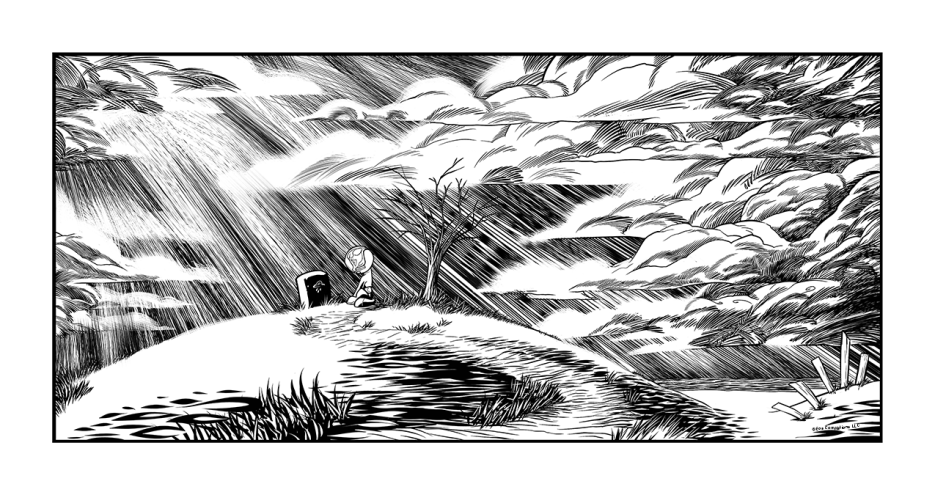
\includegraphics[width=0.9\linewidth]{image19.png}

\begin{intro}
    当风吹起时,摇篮就会摇摆,
    
\begin{englishlyric}
    When the bough breaks, the cradle with fall,
\end{englishlyric}

    \medskip

    当树枝断裂,摇篮和宝宝会一起掉下来。\footnote{这一句是经典摇篮曲 \emph{Rock A Bye Baby} 睡吧宝贝的歌词}

\begin{englishlyric}
    and down will come baby, cradle and all.
\end{englishlyric}
\end{intro}

\daytimeplace{14}{10:30 AM}{翡翠海岸,52号国道南段}{Emerald Shores, Big 52 S Branch}

帕比骑着滑板车在她的小跟班身边飞来飞去绕着圈子。

「耶……!你碰不到我!我超级快!」

尸鬼蹦蹦跳跳地想要跟上帕比,从远处看就好像两个穿着防辐射服的小孩子在嬉戏一样。不过或许这也是她们正在做的事情。一路玩耍让她们去翡翠海岸的旅程稍微慢了一点,不过这样也没什么关系。

「喏,跟班,」帕比停了下来,看着她的伙伴,「我不太确定妈妈喜不喜欢丑丑马,不过我会跟她说你是我的好朋友,而且你也找不到妈妈了,她肯定会帮你修好你的箭头……呃……不过,别做奇怪的事情好么,比如说马尾伯爵做的那种……呃……好么?我可不想第一天见妈妈就被关家门……」

那个生物歪着头,帕比把这个表情当做是肯定的回答,「那好,我来过这里好几次了,这里超超级好玩,只要你不问漂漂马太多问题就不会被妈妈训斥……问问题不是错,只是有些马不太喜欢某些谈话内容。」比如说,问为什么小马可以光屁股在大街上跑,但是为什么去海滩就必须穿比基尼之类的……帕比完全不知道为什么!

\horizonline

\daytimeplace{14}{11:00 AM}{铁砧镇,52号国道南段}{Ironworks, Big 52 S Branch}

砰……!砰……!

强盗的脑袋像个西瓜一样爆开了,在坏枪的掩护下,扳机熟练地给她的霰弹枪换着弹药。

「我们最好赶紧,乐乐,铁骑卫肯定也在附近清理……」

附近的爆炸把泥土溅了他们一头。

装好子弹之后,快乐扳机拉了一下枪栓,「没错,如果我们不想被多开几个洞的话。」雌驹说着飞奔到一座帐篷边,「掩护我破门。」坏枪移动到另一边的时候,雌驹冲进里面举起枪。

砰!砰!轰隆!

「咿!」

一堆电子设备炸成了五颜六色的火花和碎片。\thpr{打的好,乐乐,对于那些看起来像是机器的东西都是先打一枪再说。}这个帐篷里面有一张沙发,一堆箱子还有一台刚刚被她打爆的无线电……但是看起来里面一只小马也没有。

% TODO: 译文不合原文,此处改正

坏枪跟着走进来,「你愣什么呢?」

雌驹没有回答,警惕地看着周围,「我……我觉得刚刚好像听到一声惊呼……但是这里好像没有能发出惊呼的『漂漂马』。」

「那简单。」公马端起突击步枪,直接扫射了屋子一遍,在板条箱打了一排洞,打烂了小床,还把桌子上吃到一半的食物打成了一份现代派印象作品。然后他们听到了一声吃痛的惊叫,然后一个缩成一团的雌驹凭空出现在床底下,她肚子上的伤口留下一滩血。

「狗屎运……」乐乐喃喃自语,走进那个雌驹想一枪解除她的痛苦。她屁股后面有个白塔的可爱标记,那雌驹看起来那么年轻,一副失魂落魄的样子让卫兵迟疑起来。

「救救我……我还不想死……」独角兽闭着眼睛,在一阵阵剧痛带来的痉挛之间呻吟着,「妈妈……妈妈……救救我……」

「你等啥,她那样很痛苦的!」坏枪叹了口气走到那个雌驹身边举起枪。

「等等!」乐乐用蹄子推开公马的枪,她看着那个慢慢变得虚弱的雌驹,她还在祈求着她妈妈能来拯救她。

「我们……我们变成什么了?这个小马手无寸铁,只是躲在那里而已!」乐乐拿出一个治疗药水喂给她。

「你打算救活这家伙?为什么?她有机会绝对会毫不犹疑地杀了你!」坏枪不屑地打了一个响鼻,「而且她的『亲朋好友』说不定现在正在屠杀我们的盟友呢!」

乐乐回头白了那公马一眼,「你看到这个房间有任何武器么?」那个受伤的独角兽只剩下哭泣的力气了,不过乐乐还是给她喝了一些药水,「如果我们坚信,所有小马都是漂漂马,本性都是善良的,那么我们还是有机会重建昔日的小马国。」快乐扳机抱着小马要塞轻声唱着摇篮曲安慰着她。

坏枪坐在他的雌驹身边叹了口气,「你想太多了,总有一天会后悔。」

快乐扳机耸了耸肩继续唱。

\horizonline

\daytimeplace{14}{11:00 AM}{翡翠海岸,52号国道南段}{Emerald Shores, Big 52 S Branch}

帕比对面前的景象皱起了眉头,这里完全不是她记忆中的翡翠海岸!这里简直是一团糟,而且看不到一个马影!海边的所有小房子都变得脏兮兮的,而且海滩上也一片狼藉。

「怎么还没过多久这里就变成这样了?小马呢,音乐呢?婚礼庆祝呢?那些小店呢?还有……妈妈呢?」黄色的小雌驹伤心地低下了头,「抱歉,小跟班,看起来这里好像刚刚刮过台风。我想带你去玩旋转木马但是……」帕比回头用愧疚的眼神看着那个半腐烂的怪物,「我觉得现在那地方可能也没开门……」

那个尸鬼看起来毫不在意,但是帕比想给她的新朋友留下好的印象。

「哦,或许我们可以去看看糖果店好么?我们可以给妈妈准备个惊喜!」听起来是个不错的主意!给妈妈带上礼物一定能得到额外的抱抱和亲亲,「走,我们去商店血拼咯!」

小雌驹走下山丘,来到沿海的小镇上,小镇的建筑物都破旧不堪,窗户不是被打破了就是被木板钉上了,几乎城里的所有门都被木板封着。

「哇哦,刚刚过境的绝对是场大风暴!不过别担心,我知道有个买糖果的好地方!就在这个小巷子里面!」帕比一边说着,一边踩着小巷之中的水坑来到小路尽头。

「{\mt 警告,侦测到中等辐射,威胁等级:可忽略。}」

完全不管这个声音,小雌驹继续往前走着。

「{\mt 警告,侦测到大量辐射,威胁等级:可忽略。}」

帕比皱起眉头不爽地说:「喂喂,别胡说了,声音先生,拿出金币来!金闪闪的那种!我想要买好多好多糖果!」一堆金币浮到了小雌驹面前,她哼着歌转过拐角去找……

% NOTE: 补译一点

「这不公平!」

就在那个糖果店应该在的位置,现在是一个圆形的弹坑。帕比叹了口气,「好吧,好吧,别担心,我还知道很多可以买东西的地方。」不管怎么说,这里有很多很多小商店可以买好东西,怎么可能所有的商店都不见呢?

\horizonline

\daytimeplace{14}{11:15 AM}{铁砧镇,52号国道南段}{Ironworks, Big 52 S Branch}

白先生飘着一把来复枪从帐篷口探进头来。

「有谁受伤了?」

坏枪转头看着白苹果的老大说:「理论上是这样,刚刚我们打伤一个强盗,乐乐正给她急救呢。」

「哦,好吧,你们慢慢来,铁骑卫正在……等等,你说啥?」老白走进了帐篷看着那俩小马,「我们难道不就是来消灭他们的么?什么时候改变计划了?」

坏枪耸了耸肩,「你问他,好像和『漂漂马』啥的有关系。」

「闭嘴老枪,这个雌驹是非战斗成员!她只是带着隐形小马躲在床下而已,完全没有任何武器。我是个士兵,不是杀手。」快乐扳机一边说着一边用一个床单给雌驹盖好。

白先生摇了摇头,「我说,我们没时间搞这个了,野牛帮在撤退,我们必须立刻追击!我们没时间玩好马游戏了!我们越快结束这场战斗,就能越快在那个关于帕比的『阴影』什么预言落在我们头上之前赶过去。」

当听到帕比这个名字的时候,那个受伤的小马神经质地低语起来,「幽灵……是她在这个不洁之雾里召唤了不死同伴……她们是来吞噬你们的灵魂,是来杀死所有小马的!这都是我的错,我的错!为什么我要惹幽灵生气!妈妈……救命!」

「幽灵?不死?这只是个迷雾魔法而已,她在叨叨些什么?」白先生扬起了一边眉头。

坏枪清了清喉咙,「实际上,在来这里的路上,我们发现三个小马被……嗯……撕成了碎片。好像有谁用蹄子把他们给生撕了,那情景还真是挺可怕的。」

乐乐点点头,「没错,我们显然不是突袭这里的第一梯队……在我们之前,这里的小马已经在疯狂乱射了。」

白色的公马哼了一声,「真不错,这可以解释为什么还没等我们来这里就听见一堆枪声……不过现在有谁可以跟我解释她在念叨什么吗?」他戳了戳那个雌驹,「嘿,你能听到我说话么?你惹谁生气了?又是谁袭击你们了?」

「幽灵……52号国道的小幽灵……我们……不……是我……我打了她的屁股……她的泪水引来了恶魔……黄色幽灵……像她一样。但是……更残忍无情的不死怪物……她们杀了血浴……现在她们找我来了!是我打了她的屁股!是我打了屁股!全都是我的错!」

小马要塞歇斯底里地尖叫个不停,帐篷里面的三个小马一起用力才按住她。

「喂喂!冷静!这里没什么黄色恶魔!她们早走了,别挣扎,你还很虚弱!」坏枪终于坐在那个雌驹背上让她冷静下来。

「你……打了……帕比的……屁股?」白先生听到这里差点没忍住笑出来,「真的?我可是错过了最有趣的部分……」

\horizonline

\daytimeplace{14}{11:15 AM}{纪念碑镇,52号国道南段}{The Memorial, Big 52 S Branch}

「亲,你做得够好了。」

萍琪派坐在了长耳的身边。

先知长叹一声,从恍惚之中回过神来。

「我……好累……」

「亲,别担心,第一次都是这样的,不过你习惯这种感觉之后就好了。」

独角兽雌驹想要站起来,但是她的四条腿已经支撑不住自己的重量了。

「唉,到此为止了么?」

「还没……不过我觉得也没剩下多少了。亲你太过努力了,我早就警告过你,记得吗?」萍琪微笑起来,「不过别担心,一点痛苦都没有的,我们还可以一边等一边玩游戏!」

长耳露出一个虚弱的笑容,虽然死前还有个幻觉朋友可以聊天,不过在他乡异地因为毒品而孤独地死去,这个代价实在太高了——但是这一切都是有意义的。

「告诉我,她会一切平安么?」

「为什么问我?亲才是萨满哦!咱不过是个普通的漂漂马而已啦,哦,哦,你想要玩钉马尾游戏么?」

「求你了……我……我必须知道。」

叹了口气,萍琪皱起了眉头,「好吧,为啥大家全都这么无趣?好啦好啦,我说就是!她不会平安……至少现在不会,还需要最后一步,不过那个魔法迷雾相当不赖。」

独角兽虚弱地叹息,「那么,至少我死得还有价值……」

「亲,别皱眉都皱成梅干菜了!我们还要去准备派对呢!那个雾超级漂漂,把所有东西都掩盖了,帮了那些可怜的小幽灵一个大忙……至少你在最后一段旅程里给了那个小小幽灵一个可以陪伴她的朋友……不管怎么说,亲你逆转了命运!这绝对是值得庆祝的大喜事!呃……虽然把亲的小命搭上了,不过不管怎么说都应该高兴,不是么?」

……{}

「对吧?」

……{}

「哎,你看看她,又睡着了!好了!别睡了,起床了亲!我们该出发了,不然会迟到哦!」

\horizonline

\daytimeplace{14}{11:45 AM}{铁砧镇,52号国道南段}{Ironworks, Big 52 S Branch}

「你他妈跟老娘说什么?」赫瑞咆哮着,尖锐的喙几乎扎到了诘责的鼻尖,「什么叫『她不在这里』?」狮鹫完全不管其他铁骑卫对着她的枪口,继续对老书记官怒吼着。「你这个骗子!我信任你,干了你让我干的事情!现在你说她不见了?」

展开翅膀的狮鹫发出一声怒啸,对那掠食动物的吼叫毫不动容的诘责清了清喉咙,伸起蹄子示意那些铁骑卫放下枪。

「我知道我们曾经有过约定,不过她醒来以后自己跑掉了,你也知道那个孩子自个儿乱窜的时候想要让她呆在原地有多难,对吧?」

赫瑞塔眼底的岩浆似乎随时会喷发出来,「你知道现在她跑哪儿去了?」

诘责耸耸肩,「上一次见她的时候,她正往翡翠海岸去,不过我又不是先知……」

那佣兵面无表情地说:「我猜,她往南走了是吧。」

铁骑卫点点头,「就在海边,错不了。」

孤狼从旁观的马群里面走了出来,「等等,狮鹫,你想去那边的话,我和你一起去!」雄马展开翅膀跟上了赫瑞塔,「我觉得我们应该等等其他马,那里可能会有危险!」

「没错,等等,老娘等够了。在你们整个肏蛋奇蹄类动物里面,老娘只关心一位,而那位现在不在场……滚边儿去吧,小马!」赫瑞塔啐了一口,就好像要吐掉喙之中的恶心味道一样,然后张开翅膀消失在工厂屋顶之后。

「我现在就去追上她,你们尽快跟上我们好么。」

白先生以蹄覆面,「真是个好计划,先是单独行动,然后又是添油战术么,难道不是有什么南边的邪恶黑影啥的预言么?我们已经把我们那花里胡哨的专家丢在脑后了,现在又要分开行动。要我说,我们还是检查一下这里的生还者,然后决定怎么处理俘虏,最后等长耳来了一起往南走好么?」

「说到往南走……有谁看到融金了?」快乐扳机看着周围问。

天马嗤之以鼻,不耐烦地刨着地面,「这里有天杀的十五个铁骑卫!十五个!这群家伙绝对可以解决土匪的残兵败将,然后帮下面那些小马打开避难厩!现在我更关心那个幽灵而不是52号国道的地盘划分!我去追那狮鹫去了,你们最好也快点!这可不是个会等你们的派对,如果先知没错的话,我们时间不多了。」留下这几句话,孤狼飞走了。

\horizonline

\daytimeplace{14}{12:00 AM}{翡翠海岸,52号国道南段}{Emerald Shores, Big 52 S Branch}

帕比一点都不开心,她完全没找到任何给妈妈的礼物。或者说,她在整个城里连一只小马都没找到,这让她开始紧张起来。小雌驹觉得哪里不对劲,她开始担心妈妈会不会又跑到另一个地方去了。

所以她急忙冲向那个粉色箭头指向的海边小山丘,帕比在城里闲逛的时候,那个箭头一直没变过,不过帕比以前也遇到过这种事情,每一次旧的箭头消失就会有新的箭头出现,一次又一次地出现。

「好吧,小跟班,我们去找妈妈,或许这一次是对的!」

两个小孩子慢慢爬上泥泞的小小山路,这个山丘有一片微枯的黄绿色草坪,还有一颗死去很久的老树,帕比来到山顶的时候,她看到那里也有很多很多的小石头,每一块上都刻着一个名字和可爱标记,就像另一个爸爸的地方一样……好奇怪啊,为什么会有另一个爸爸的地方?

一只小马正坐在那颗只剩下枝干的树下,他慢慢站了起来,走向帕比和她的新朋友。

小雌驹飞奔向来者。

「妈咪!」

帕比的声音里充满了希望,但是很快又变小了。

「你……不是妈妈……」

在帕比身后的小跟班冲着来者发出了威胁的低吼声。

「不,帕比,我不是你的妈妈,抱歉……」融金用他那沙哑的声音说着,然后走到了一个布满苔藓的灰色石头面前,

「我真的……很抱歉……」

小雌驹走到了那个尸鬼身边,然后注意到那个粉色的箭头原来是指向这块石头的。虽然石头上的字迹早已经风化得模糊不清,不过她可以清楚地看到,那个一朵云和三点雨滴的可爱标记。

那是……妈妈的……可爱标记。

妈妈……{}

\horizonline

\daytimeplace{14}{12:00 AM}{翡翠海岸,52号国道南段}{Emerald Shores, Big 52 S Branch}

「好了,都安排好了。」白先生和诘责一起走了出来。

快乐扳机点点头。「好吧,那里一点都不远,我们别磨蹭了。」

诘责看着远处那个指示翡翠海岸方向的标志牌,只有六公里而已,天气好的时候都可以清楚看到小镇。

「如果那里情况不妙的话,我们要尽可能地拖延时间。」

「那还不赶紧!」快乐扳机说着沿着52大路开始向南边飞奔。

「好吧,谁最后到谁就是赤兔!」灌木笑着看了他叔叔和老书记官一眼,然后跟上那雌驹的速度。

诘责叹了口气,「这帮小年轻,他们绝对会在半路就累趴下的。」两个老公马跟着其他小马一起奔向海岸。

\horizonline

\daytimeplace{14}{12:10 AM}{翡翠海岸,52号国道南段}{Emerald Shores, Big 52 S Branch}

尸鬼什么也没说,只是静静地站在那里,让帕比有时间理解这个现实。

「妈妈……在这里?但是……」

小雌驹盯着这块石头,想要理解到底发生了什么,而跟班则坐在了头领身后。

「她……和爸爸……走了?但是……但是……不……不要……」帕比的声音越来越小,好像她声音太大的话,这个残酷的现实就无法改变一样。

「但是……我……我也想去……我……我想去见爸爸……为什么……为什么她把我留在家里?我……我……」

帕比失声痛哭起来。

「我真的没有不听话……我只是……我只是想要看烟火!我……我不知道我的房子会倒掉我妈妈会走掉……我……我……」帕比一屁股坐在了地上,低头看着自己的蹄子。

「只是想看那个破烟花而已……为什么接下来一切都一团糟!我很抱歉……我错了……我真的错了……对不起……妈妈……请回来呀!」

帕比嚎啕大哭,绝望地对着那块埋葬着她母亲的墓碑大声哭道:「妈妈!你……你说什么我都听!训我吧!打我吧!但是别扔下我啊!」

融金看着他面前的可怜生灵,想要说些什么,说任何事情,但是这一幕实在太过悲哀,让他说不出一个字。而这个时候,她抬起了头,于是那双泪流不止的双眸和他对上了。

「求求您,求求您告诉我妈妈去哪儿了!我把我的玩具给您好吗,我愿意把我所有东西都给您,好吗?还是您想要更多漂漂玻璃珠?我会为您把所有的玻璃珠都找到,好吗!求求您!求求您了!」帕比站起来走向那个老尸鬼,而小雌驹沉重的视线让他不由得后退了几步。

「帕比……我很抱歉,但是……这里就是你妈妈长眠的地方……她……已经死了……她很久很久之前就已经去世了。」

帕比笑了,但是那微笑毛骨悚然。那双空洞的眸子盯着融金,不住地颤抖着,「死了?只是死了?她死了?那没关系的!她会好起来的吧!我也已经死了,但是你看我很好啊!你也死了但是你也很好啊!死了没什么不好的对吧?我们只要在这里等就好了,对吧?对吧?对吧!」

融金看着那天真的小孩子,死了……还会好起来?只要在这里等?

「帕比……不是这样的……她……她已经不会回来了……她已经去世了……她已经……帕比……你可以跟我在一起,好么?我永远不会丢下你。虽然我不是你妈妈……」

「怎么有俩帕比?到底发生什么了?」赫瑞塔一个猛地降落在地上,压坏了好几根树枝。「僵尸,把你的脏蹄子从我朋友身上拿开!」狮鹫落在融金和帕比之间举起枪指着尸鬼。

黄色的小雌驹很快就认出了新来的狮鹫,「赫瑞!赫瑞!妈妈……妈妈……妈妈她……妈妈她不要我了……她和爸爸走了……丢下我不会回来了……我……我我……帮帮我!」

佣兵看了看那个用蹄子指着墓碑的尸鬼,然后明白了帕比在说什么。

「肏你妈,老娘……来迟了……」

赫瑞塔转身用一只爪子抚摸着帕比的头盔,「帕比,我会陪你,好吗?你不会孤独的。」

「但是……我想我妈妈!我要我妈妈!她……只有她才能……只有她才能把一切都修好!她可以修好坏掉的房子,修好这个破太空服,找到跟班的妈妈,让之前快乐的日子再回来!没……没有她我都不知道该怎么办!」

什么也没说,狮鹫紧紧地抱住了帕比。

「但是……但是你自己就已经做的很好了,帕比……你救了我,你还救了整个太阳城!你还阻止了铁骑卫的内战!你还……你……你是个好孩子!你是我认识的唯一一只好小马!不需要你妈妈,你就可以解决一切。让我当你的姐姐,好么?赫瑞和帕比,最佳组合!」

「狮鹫说的没错,帕比……你已经长大了,你妈妈会为你自豪的。」

帕比挣扎着推开了赫瑞塔,她的双眸之中燃烧着粉色的火焰,「但是她把我丢在这里!她扔下我和爸爸一起走了!我那么爱她,为什么她要扔掉我?为什么她不爱我?」

「你丫到底想……」赫瑞塔摇了摇头,「你到底说什么呢?她没有选择扔下你,她只是迫不得已。她绝对不会丢下你不管,她以为你在避难厩里面会平平安安的长大,否则她绝对不会把你丢在这么危险的地方的!」

孤狼落了下来,「呃……我不知道发生了什么,但是我觉得对小孩子大喊大叫没什么用。」

「我说也是,狮鹫小姐,所以我一直不……」

帕比打断了那两个公马的碎碎念,大声吼着:「那么为什么她不回来接我一起去?」

「傻瓜,她已经死了!死了!懂不懂!」赫瑞塔锋利的喙顶着帕比的头盔,和小雌驹对视着,融金想拉开狮鹫,但是小跟班低吼着拦住了他。「妈妈不会再回来了!你已经永远失去她了!这就是命运!她现在就躺在这个坟墓里面,绝对!再也!!不会!!!回来了!!!!所以你要坚强起来,将你自己的命运踩在蹄下!别管那破墓碑了,现在就跟我走!」

狮鹫转头看着那个老木乃伊和天马,不过她马上注意到一大堆小马正在从北边赶来。

「看到没有?你的朋友来接你了!你让大家都担心坏了,别再这样失落了,伸出蹄子站起来好么!」

帕比看了看过来的马群,然后又看了看那个有可爱标记的墓碑。

「妈妈……在这里面?」

赫瑞塔完全没有注意到帕比的表情和融金拼命的示意,只是说着自己的话,

「没错,你妈永远都躺在这里,你什么时候想来看她都可以,现在跟我来,一起和你的朋友说你一切安好,好么?」

「石头!」

帕比尖叫着举起了「命运之石」,然后用力砸向那个墓碑。

「你丫在干什么?」赫瑞塔想阻止她的朋友,但是小跟班跳到了她们俩之间,即使是勇敢的狮鹫也被那双红色的眼睛吓住了。

「妈妈,妈妈出来啊!」帕比用她所有的力气砸着墓碑,融金和孤狼被这碎石飞溅的景象吓坏了。

「等等孩子!那样她也不会回来的!别这样,你会……你会打坏你妈妈的坟墓的!」孤狼跳了起来落在石头边挡住了帕比的蹄子。

「你到底怎么了?别这样!」

「放开……放开我……放开我!我想要妈妈!为什么妈妈不见了!」

跟班转头吼着天马的时候,赫瑞塔立刻冲过来打上帕比的头。

「傻瓜!给老娘振作起来啊!丫的真想打你的屁股!忘了你妈妈吧,傻瓜!你现在和我在一起了,别想不可能的事情,醒醒吧!」

被狮鹫的愤怒搞迷糊的帕比愣住了,小雌驹慢慢地转向大海,「但是……但是……我把她忘掉的话……我找不到妈妈的话……我……还能做什么呢?」

赫瑞挥着爪子说:「那我们就一起去找些快乐的事情来做,好么?你冷静下来,我会替你想办法的!乖乖的……乖乖的坐好……你看,你的朋友都在这里。」

老白,诘责,快乐扳机和坏枪正跑向山丘,虽然他们看起来精疲力竭,但是诘责还是喘着粗气问。

「发……发生什么了?」

帕比看了一眼蹄子中的「命运之石」,低声说:「我……我不想醒来……我只想……永远睡下去……再也不醒来……」

赫瑞塔拍着帕比的头盔微笑着:「我知道那种感觉……但是,总有一天会消失的,你也一样……乖乖坐在这里冷静一下,我们去招呼新来的小马,好么?」

黄色的小雌驹虚弱地点了点头,「命运之石」第一次从她蹄中滑落,滚下山丘,在山坡上来回弹了几下,最后随着一声金属敲击声落在了海滩上。

\horizonline

\daytimeplace{14}{12:25 AM}{翡翠海岸,52号国道南段}{Emerald Shores, Big 52 S Branch}

融金和孤狼已经走向了新来的马群,赫瑞塔也走了过去,把帕比和她的黄色小伙伴孤零零地留在坟墓边。

「别担心,她会好起来的,她现在只是需要独处一会儿。」

「但是……她在哭么?她怎么样了?」

帕比觉得如此……空虚。不是悲伤,也不是愤怒,也不是她以前感觉到的任何感情。她就在她妈妈面前,但是妈妈却不在这里,再也不会抱着她,对她微笑了……{}

「……虽然我不是那么多心,但是我还是想看看她的情况……」

「……那小心另一个尸鬼,那东西看起来蛮凶的……」

大家都在乱糟糟地说着什么,在帕比听来就是一阵嗡嗡的声音。帕比不关心,她只是慢慢地沉浸下去,慢慢地沉入内心深处。

再也见不到妈妈了。这个想法已经让她失去了所有力气,她顺着这条路走了这么远,唯一的目的就是想要再见到她的妈妈,但是现在什么也没有了。她很喜欢她的朋友,但是她觉得这样不对,这里根本不是她应该在的地方,她根本就不想呆在这种地方!或许……或许会有什么地方……不一样的地方……更好的地方……{}

「……那么就是这样了?我们做到了?52号国道安全了?那孩子也没事了?好了,我们现在回家吧……」

回家……家又在哪里?家已经没有了,她在中心城的家已经没有了,妈妈已经没有了,再也回不来了,再也见不到她了。帕比不想这样活着,她不想要这样……每一天晚上都醒着,直到凌明的曙光再一次提醒她又是没有妈妈陪伴的一天……她不想醒来,只想就这样睡去。

\pypr{「哦,那很简单,小家伙,你只要和我许个愿,我就会让你静静地睡去,做一个永远永远不会醒来的美梦。」}

「……闭嘴老枪!我们离开几天而已,隧道镇又不会烧了!」

「真的?你能做到么?」

\pypr{「那当然!我可是梦之主,我可以给你所有的快乐,你只要向我许个愿。」}

「……野牛帮还没完,我们只是把他们赶走而已,但是我觉得我们应该想出一个和平解决方案……」

「……我不觉得他们会同意的,老爸,野牛帮可不吃爱与宽容那一套……」

「……或许现在他们的王牌都打光了,他们会更……讲理……诘责,我觉得我们至少应该试试看……」

「永远永远的永远?」

\pypr{「比永远还要更长久,这是你我之间的约定哦。我可以让你在梦中和你爸爸妈妈永远过着幸福快乐的生活,而你嘛,只要让我在你睡着之后做一点点小事就好啦,可不可以啊?」}

小跟班尖叫着拼命戳着融金的后背,但是大家似乎全都更加专注于老白和诘责之间关于52号国道将来格局的讨论,没有注意那个小小的中心城尸鬼。

「我在52号国道混了这么多年了,我记得野牛帮最早可不是那么凶恶,他们只是52号国道上的游牧民,只是因为52号国道的每个居民点都对他们课以重税,但野牛帮在重税之下买不起任何他们想要的补给,所以他们才铤而走险……如果每一个族群都友善那么一点,也不会落得如此结果。」

「……我可不那么想……我祖父总是说野牛帮一直在找机会咬你一口……」

% TODO: 如何修正这里?

「……第一个对野牛帮课税的就是老白你祖父!你难道一点想要改变这个的常识都没有么?」

一声悠长的叹息,帕比点点头,「好的,就那么做吧!」

\pypr{「你的选择很正确,你绝对不会后悔的。」}

「做什么啊,帕比,我虽然很喜欢你,但是废除马头税可没那么简单,大人说话小孩子别插嘴好么!」

「对,没错,请……让这一切都消失吧。」

\pypr{「我真是太喜欢你的天真纯洁了……我会想念你的,来吧,请闭上你的眼睛……」}

~\vfill

\begin{note}
    升级(Lv 18)

    新技能解锁:就是现在!——你立即升一级。

\end{note}

\begin{note}
    升级(Lv 19)

    新技能解锁:专注射击——在S.A.T.S.状态下,你瞄准对手的特别部位时得到5\%的命中率加成……你想说啥,帕比已经绝望到开始胡乱选专长了,她根本没有S.A.T.S.!

    新任务专长解锁:移动梦魇(等级3)——耶!你现在就是梦魇了!不过这对你的社交生活没什么好处,因为你对所有派系的声望都变成了敌视。至于属性奖励就不在这里写了,因为太长写不下了。
\end{note}



\chapter{路之尽头}

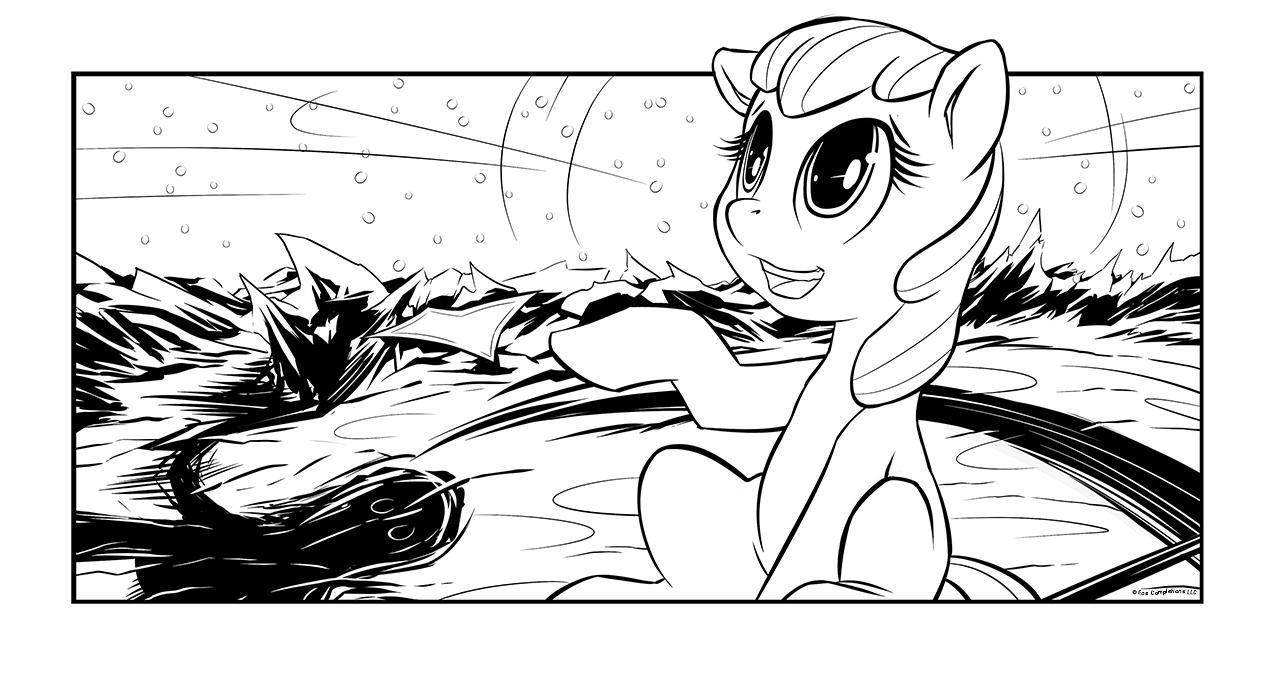
\includegraphics[width=0.9\linewidth]{image20.png}

\begin{intro}
    派对结束的时候,大家一起来个大拥抱吧!
\end{intro}

\daytimeplace{14}{12:35 AM}{翡翠海岸,52号国道南段}{Emerald Shores, Big 52 S Branch}

在拍打着海岸的阵阵波涛声中,帕比孤零零地面对着墓碑,而她的朋友在不远处争吵着。不过她唯一听到的就是在她脑中的低语,那个承诺给她美梦的低语。

「对,没错,请……让这一切都消失吧。」

赫瑞塔模模糊糊地听到帕比在她身后的低声念着,然后忽然感觉到一阵莫名的寒意,就好像刮起了一阵阴冷的夜风……她忽然觉得小雌驹刚才说的话有点不对劲。

大家全都回头看着快乐帕比,她在自言自语什么呢?消失?怎么消失?

赫瑞塔走过去,她可以看到帕比低着头闭着眼睛。小雌驹的鬃毛已经从之前的金色完全变成了夜空色。

「帕比?你还好吗?我……我觉得你鬃毛是不是有点……」

当帕比再一次开口说话的时候,却是另一个完全不同的声音,深沉而阴森,就好像在洞穴深处不断回荡的呼号。

「本宫终于亲临这个世界了,吾卑微的子民,还不赶紧对汝之新公主跪拜行礼!」

赫瑞塔歪着头挑起眉毛,「你丫说什么乱七八糟的,帕比?搞什么啊?」

小跟班的眼睛从红色变成了蓝色,慢慢走到帕比身后,像个卫兵一样笔挺地站着。那个黑化的帕比又说话了。

「本宫可不是快乐帕比,本宫乃星之子,怕音!汝等蝼蚁之辈的新公主,本宫将领导小马国崛起!」

诘责摇了摇头,看着融金问:「星啥?听起来像是某种上古斑马故事,星星什么的?」

老书记官的问题被赫瑞塔的暴笑打断了。

「怕音?你这个大反派的名字也太寒酸了吧,怕音是什么东东啊?你是自己想的么?」

羞得满脸通红的黑化帕比后退了一步,不过很快就恼羞成怒地大喝起来。「名字……名字什么的……收声,不准笑,愚民!这是汝等新公主之大名,还不快给本宫跪下!然后回到尔等故乡去宣布本宫临幸这个世界!」

快乐扳机嗤之以鼻,往前跨了一步,「不然呢?」

在怕音眼中的夜空色光芒一下子扩展到了小雌驹的全身。在她头上形成一个尖角,同时在背后展开了一对虚无的翅膀。

「不然,本宫会吞噬汝等灵魂!」

乐乐呆呆地看着那雌驹,而孤狼低声问诘责:「她能吃掉灵魂么?」

书记官看了看DJ,耸耸肩,「我怎么知道,如果她真是某种斑马黑魔法的产物……大概可以?不过我觉得她现在还没那么强。」

天马冷笑一声,「那就是不行啦?」

「并不全是,她还在显现阶段。你看她的翅膀和角还都只是虚影,而我想我知道怎么结束这场闹剧。」

在乐乐和那个生物对峙的时候,书记官低声和其他小马商讨着对策。

「我想我可以切断那个星灵和帕比的灵魂链接……如果怕音……呃……那东西没有灵魂以供给养,她就没办法在这个世界显现,自然就会被放逐回星界。」

「那么,你还等啥,邀请函么?」尸鬼问。

「不,我没办法自己施展这个魔法,这是一个又强大又复杂的法术,是一种超聚魔法,需要多个独角兽来施展……」

老赏金猎手说:「那么,你是想说,我们要被这个有这么孩子气名字的逗逼日翻了么?」

「喂,怎么,你们这些书呆子有什么好办法没有?」老白的脑袋挤进这仨小马围成的圈子中。

「技术上说,有,不过我需要几分钟搞定细节问题,帮快乐扳机让怕……这名字实在是……唉。」老书记官以蹄覆面,「好吧,反正让她忙着聊天,给我们争取点时间。」

老白点点头,然后走向另外仨马——赫瑞塔,坏枪和快乐扳机。

「我说,公主殿下,您刚才好像说了什么小马国崛起啥的?您可以详细说明一下如何做到么?别在没用的地方磨嘴皮了。」

梦魇暂时放下和赫瑞关于白痴名字问题的无营养争吵,转向新来的小马。「那易如反蹄,本宫的魔法比此等鼠辈强大万倍,本宫可以用法术治愈这腐朽的大陆,然后翻开小马国的新篇章!本宫决不允许吾之子民相互伤害,汝等粗鄙之辈的血腥争斗将被画上句号,汝等应该为本宫建造宏伟宫殿。汝只要为本宫送上贡品,而本宫将会解决汝等的一切问题!」

老白点了点头然后说:「好吧,听起来像那么回事……不过……你刚才说过贡品什么的是什么意思?」

那圣灵得意地坐下来,眼睛都乐得眯起来了,享受着被顶礼膜拜的快乐,「那是当然,本宫作为汝等的主宰。自然会要汝等做出一些……牺牲。嗯……每次满月的时候,每个城市献上一位小马做祭品就可以了,然后本宫会净化这片大地,保证汝等在本宫的统治下衣食无忧!」

乐乐皱起了眉头。「你……你要活祭做什么?」

怕音挥了挥蹄子,「和汝等无关。」

赫瑞和乐乐都惊得张大了嘴。雌驹正准备举起枪的时候,她注意到了老白的暗示又放下了。

这时候赫瑞说话了:「那么……你会把帕比还给我们么?」

梦魇有些惊讶的眨了眨眼睛,「什么,她才不会回来,在谁也不能伤害到她的地方,她正安享美梦,此乃吾等之约定!」

听到这句话,乐乐顿时大怒:「你说啥?帕比那么天真的孩子你都要骗,你的那些美梦全都是不存在的幻影!你……你居然欺骗一个孩子,骗她把美梦当成现实!放她回来!」

那怪物大笑起来:「汝等可笑至极!为何本宫会放弃如此甜美的灵魂美味,在她母亲陪伴的美梦之中,她将会长眠,从此彻底消失,这个残酷世界再也不会伤她分毫了。本宫绝不会再让那个孩子被你们所谓的现实所伤害。所以,那孩子将长眠不醒。另外,本宫特别开恩,提拔诸位成为本宫的信使,汝等现在就去小马国告诉子民本宫的驾临吧!」

「简而言之,」赫瑞抬着头,「你就是梦魇之月?」

「嗯,本宫尚未……好吧……正是……本宫是说……梦魇之月乃是比本宫更加古老而强大的前辈……」那个圣灵似乎陷入了沉思,不过马上又抬起头来,「不过本宫也足够让汝闭上那臭喙!」

赫瑞塔冷笑不已,「那么,简单的说,你丫还是个菜逼。嗯,梦魇菜逼。」

快乐扳机被这一句话逗得再也忍不住了,捂着肚子在地上笑得打滚,老白以蹄覆面,而其他三个小马回头看着这边,很好奇发生了什么。

「不准笑!本宫生气了!这个世界有这么多子民,本宫才不需要汝等……一……二……呃……反正很多个无用的笨蛋!」

赫瑞塔嗤之以鼻,「……你丫连四都数不到,就别装逼了好么?」

「汝……汝这个……蠢材!汝将付出代价!」

「不,她才不会!怪物!看招!」诘责站在了赫瑞塔面前,直视着梦魇的双眸,「以科学之名,我们会将你永远放逐!」

「哟呵?」那怪物咯咯笑着,虽然还气得满脸通红,但仍然不屑地挥了挥蹄子,「别逗本宫发笑了,科学?汝等是否明白本宫乃是何等存在?看在梦魇之月的份上,别说梦话了好么?」

诘责微微一笑,「你想听细节?好吧,仔细听好,我之前早就检查过帕比的防护服了,你能在这里显现的原因不过是因为某个呆瓜把死灵法术当生命维持法术用而已。不过我已经知道怎么纠正这个可怕的谬误了。虽然那魔法晶片几乎坚不可摧,但那里面的魔法却没那么稳定,这就是为啥你的翅膀和角还都只是虚无的火焰。不过现在这里有好几个独角兽,虽然他们不懂啥叫『魔法裂解术』,但我可以直接使用他们的魔力来施展这个超聚魔法。那么,现在猜猜看这个『魔法裂解术』要用在谁身上呢?」

「什……什么……?」那个梦魇大惊失色,后退几步。

「好了各位,我要准备法术了,你们只要放空脑子让我接管你们的力量,然后这场梦魇闹剧就此结束了!」

一道闪光从诘责的角尖上炸开,光芒跳跃到几个独角兽的角上,他们都一起将那个魔力聚集起来为超聚魔法添加魔力。

乐乐闭上眼睛,让魔力透过她的身体,然后坏枪和老白也一起做了,很快他们的角也一起发出同样炙热的光芒,照亮了整个山丘。

赫瑞塔被这强光逼得微微后退闭上眼睛,不过诘责刚才说的话让她很担心,他打算摧毁那个防护服上用作生命维持的死灵法术来毁灭那个梦魇,但那不是让帕比活着的东西么?

赫瑞塔转头对老书记官大叫着:「等等!你想杀了帕比么?」

诘责没有回答,但是被白光照亮的那个怪物惊恐的尖叫让赫瑞确认了自己的担忧。

「愚蠢之辈,如果你解除那个魔法,那孩子会和我一起死的!」

「不行,肏蛋!给老娘停下!你不能杀了帕比,天杀的独角兽!」赫瑞塔怒吼着冲向诘责,把他撞飞了出去,诘责仰面朝天地摔倒,失去了法术的专注。

那个白光射出的彩虹失去了焦点,飞得到处都是,就好像一个坏掉的迪斯科彩灯一样到处飞。

梦魇菜逼或者说怕音,小心地睁开眼睛,不知道发生了什么,不过看起来自己毫发无伤,看着面前几只满脸莫名其妙的小马,她的脸上露出了邪恶的微笑。

「哈……不管怎么说,帕比的狮鹫朋友最后还是有点用处的。下次挑战本宫之时,汝等还是别拉这种猪队友入伙了。」怪物大笑着:「噢,本宫说什么笑话呢,汝等已经没有下次了,因为汝等鼠辈现在就去死吧!」

诘责摇摇头站了起来,被赫瑞塔刚才那一撞搞的莫名其妙,「你……你为什么要打断魔法!你这个脑子里塞羽毛的蠢货!那法术就要完成了!」

另外几个独角兽也满脸恍惚,显然是被强力魔法的消耗搞得精疲力竭。融金正在推醒老白,赫瑞塔则冲向诘责,用爪子指着他叫着,「你……你不能把帕比从我身边带走!一定还有其它解决办法的,绝对会有的!」

「蠢货!那孩子已经死了!我们是在拯救52号国道!从你那快乐结局的美梦中醒来好么!」诘责怒斥着狮鹫,因为他们决胜的王牌被她给搞砸了,这样会害死很多小马。

梦魇享受着她对手的胜利美梦破灭的瞬间,「汝等的争吵何等有趣,本宫还真想再多欣赏一番,看鼠辈的丑恶内讧也是不错的消遣。不过现在本宫很忙,还有个王国要去统治。」怕音看了看双眸已经完全变成深空蓝色的跟班,那个中心城尸鬼已经变成了她忠心耿耿的侍卫,「游戏就此开始了。去吧,我的爪牙,教训这个臭嘴小鸡!」

跟班像猫扑老鼠一样扑向赫瑞塔,正在和诘责争吵的狮鹫完全没有注意到冲上来的尸鬼,甚至都没听到乐乐的警告。

尸鬼撞上狮鹫,扭作一团从山坡上滚了下去,赫瑞本能的反抗着,她的动物本能让她躲开了那小孩子强大的超自然力量,并且快速地反击着。他们化作一团蹄子和爪子的残影摔落到下面的海滩上。

看着她的爪牙和狮鹫滚出了视线,怕音叹了口气,「好吧,坏小鸡弄坏了我的玩具,看起来本宫还是自己动蹄……那么,谁想先死?」

孤狼和融金交换了一下视线,然后快速地跳起来把弹夹打空,子弹就像穿过黄油一样打穿了梦魇的身体。

帕比的胸口被打成了筛子,但是看起来完全没有用,因为下一瞬间那些洞都消失了。

「想要杀一个已经死掉的生物,是不是有点难度?」

怕音咯咯笑着用魔法抓起孤狼,然后把他扔向了一棵树。那天马重重撞在树桩上,随着一声黏黏糊糊的骨折声,倒在了地上,整个身体都向后弯折成了一个诡异的角度。

不过梦魇没有理会孤狼是不是死透了,转头面对着坏枪,「本宫看到汝还是拖家带口的来,何其可爱。汝等是想和那些老掉牙的戏剧一样『但求同年同月同日死么』?汝等有何遗言?」

「有,」老白举起包包里面的步话机,打断了怕音,「B计划,」他眯起了眼睛,「我们叫兄弟!」

远处传来一声炸雷,随之一发精确的狙击打穿了帕比的头盔,还轰掉了她的一条腿。

受伤的梦魇怒号着张开翅膀,飞上天空从云中招来闪电,雷霆如利剑般击中了远处的摩天轮,那个巨大的马造钢铁建筑在一阵烟尘之中轰然倒塌。

「不!灌木!」老白看着他侄子之前在的狙击位置已经成为一片废墟,这个……他完全没有想到会发生这种事情!

一排地对空导弹拖着长长的尾迹飞向天空中的梦魇,然后在她身边爆炸成无数火球,照亮了整个昏暗的天空。在他们的掩体之中,每一位铁骑卫都举起了他们的武器,向怪物的方向开始狂轰滥炸。

战斗开始了。

\horizonline

又黑,又冷,又湿,赫瑞塔呻吟着,她全身的骨头都在哀嚎,她完全不知道发生了什么,就记得有什么事情不对头。

在一阵粉色光芒中,有个甜甜的女声在低声耳语。

\emph{「亲,别担心,不过是你这个大坏蛋又干坏事了……没别的!」}

「坏啥?我死了?」狮鹫头疼得更厉害了,远处可以依稀听得到小马的尖叫声和爆炸声。但她可以清楚地感觉到,有什么东西,像是个粉色圆点,在她脑中跳跃着。

\emph{「笨笨小鸡,亲还没死呢。只不过是从六米高的高度大头朝下掉下来然后倒栽葱撞到烂石滩的后遗症而已啦。不过我可以肯定亲一点伤疤都不会有的!黛茜酱天天这么坠机也完全没有事!」}

「帕比?她怎么样了!我要救她!」

那个粉色圆点跳了跳,语气听起来就像是大姐姐在教训小孩子一样。\emph{「真的吗?但是看起来亲只是想要满足自己而已嘛!」}

「你……你他喵的叨叨什么鬼!我只想让她安全!」

\emph{「然后呢,让她永远永远都陪亲么?亲到底是想救谁,是可怜的小帕比,还是孤单的小赫瑞?」}

「老娘……我……我不知道……我只是想让她开心,让她露出笑容!她是如此特别,就像整个灰暗世界的一抹艳丽的色彩……我不想失去她,但是她除了自己妈妈什么都不想……就像……活在一个噩梦之中。」

\emph{「或许,她只是在做一个不知道如何醒来的美梦。或许,她需要她最最最要的朋友给她一点点点帮助。」}那个声音开始变化了,从一开始年轻雌驹的声音变成了一个老马的声音,但却又无比熟悉,让她想起来了太阳城那几天。\emph{「只剩下最后一步,找到帕比的「命运之石」,然后完成它的使命。」}

深吸一口气,赫瑞塔睁开了眼睛,发现自己正躺在乱石滩上。不远处是一个摔得粉身碎骨的太空士官长小跟班。那个生物似乎吸收了他们俩坠落的所有冲击力,现在就像一颗压扁的黄色橡皮糖一样贴在地上。赫瑞举起手枪,给那东西脑袋上补了两发,确保它完全死透彻了,然后检查周围。

在她头上,有一只小马被梦魇的夜空色魔法包围着,惨叫着飞出两百多米,然后啪叽一声栽进海里。

赫瑞没有理会那些上面那些战斗的喧嚣,给自己灌下一瓶治疗药水,开始找那块破石头。

「帕比的石头,帕比的石头!他妈的老娘怎么从这么多破石头中找一块石头?命运你妹的石头!」狮鹫恼怒地踢飞一块石头,那石头飞向一个生锈的铁盒子之后反弹的飞起来,在空中打着转,然后不偏不倚正中狮鹫双目之间。

「肏!」狮鹫一边揉着她的脑门一边捡起那块石头,她记得这块石头打中自己的声音,「这是你丫最后一次砸老娘的脑袋……然后……然后该干啥?你打中一个金属盒子,破石头,你想说啥?你是某种石头先知么?」赫瑞塔骂骂咧咧地走向那盒子,然后用「命运之石」砸向那盒子上的锁头。

「终于……」

咣!

「你丫……」

咣!

「还算……」

咣!

「有点用!」

咣当!

「很好,我们看看宝箱里面藏了什么?」

里面有几张纸片,一个老旧的阿杰玩偶,一些照片,赫瑞拿起照片看着他们。

其中之一是快乐帕比,不过稍微小一点,而且没有穿防护服,她正在插着四根蜡烛的大蛋糕面前开心地笑着,后面还有一些小马,看起来像是一个生日派对。

第二张照片是一个白色公马和紫色雌驹,他们站在一个老木牌面前,看起来他们是在苹果鲁萨门口,在两个小马之间坐着一个噘着嘴的快乐帕比,好像她不想拍照片或者完全不想去那里的样子。那个小雌驹看起来很年轻,或许只有三岁的样子……赫瑞塔转过照片,背面有一行字:「最后一次全家旅行。」

第三章照片是帕比穿着一件罩衫,带着一个蓝色的大大蝴蝶结,她正开心地笑着展示自己的新裙子,这一次在前面写着字,「帕比第一天去幼儿园」。

在最后一张照片的背面,年轻的佣兵发现后面写着这几行字。

\medskip

\wrpr{不管在哪里,不管是什么时候,在那遥远的彼端,我们会和爸爸再一次相聚。我以你为傲,妈咪永远会喜欢她的小小太阳。}

\wrpr{我爱你!}

\begin{flushright}
    \textbf{妈妈}
\end{flushright}

\medskip

一发导弹凌空爆炸,闪光照亮了赫瑞脸上流下的两行泪水。

佣兵叹了口气,终于抹去了模糊了双眼的泪,「她……她不属于这个地方……」赫瑞塔放下这些照片,「肏他娘,为什么要这样?为什么?!」

新的爆炸将天空染得火红,小马在那里和已经死去的东西战斗着,不断地死去,只是因为她自私地想要把幼驹留在自己身边。现在赫瑞知道自己该做什么了,虽然,这不意味着她真的想要这么做。

「不公平……这不公平……」

\horizonline

帕拉丁高斯瞪大眼睛,看着他发射的导弹在空中掉了个头,又朝自己飞了回来。

「高斯!」冷浴惊恐而无助地看着她最好的朋友在爆炸中消失,她愤怒而痛苦的视线转向梦魇,「臭婊子,为什么你不去死!」在她动力装甲两侧的转轮机炮疯狂地喷射着火舌,但是即使她打光了子弹,那个怪物也只是狂笑着把另一个新兵丢进大海。

怕音已经杀了两个铁骑卫,还把好几个小马丢进了大海,不过怎么才能一劳永逸地消灭这些家伙呢?这些笨蛋真的不知道什么叫决斗的规矩!她现在开始有点不耐烦了。虽然说杀掉小马很有趣,不过现在看起来这些家伙简直烦不胜烦,前仆后继根本杀不光的样子。而且她现在可有更重要的事情要做——比如说,统治世界之类的。

那么擒贼先擒王,这些蠢蛋的老大是谁呢?哦,对了,那个老书记官……怕音因为自己的小小邪恶脑瓜而坏笑着,「我说,穿披风的家伙在哪儿啊?」怕音落在老马的面前,张开她夜空色的翅膀邪笑着,「在这里啊,诘责,是吧?」就在那独角兽因为小雌驹心情突然变化而奇怪的时候,梦魇的笑容变得无比凶恶,「那么,去死吧!」怪物用魔法抓起老马的心脏,然后用力一捏,诘责闷哼一声倒了下去。

这个时候,赫瑞塔从悬崖边飞了上来,落在小山丘上的墓地边,面前的景象让她心中一紧。这都是她自私的错,小马在战斗,小马在死去,帕比绝对不会想要这样,该是结束这一切的时候了!

「帕比!帕比!听我说!」

不耐烦地叹了口气,梦魇转向狮鹫,「我说,还没轮到你呢?知道先来后到吗,等我先把这个杀掉之后再来杀掉你,别着急行不行?」

快乐扳机艰难地爬向诘责,卫兵雌驹绝望地想把老书记官救活过来。他们的抵抗就像纸片一样被小孩子扯得粉碎:融金正在那根穿透了他身体的树干上拼命挣扎着想要脱身,孤狼早因为脊椎骨折而昏了过去,即使是那些精锐的铁骑卫也被打得节节败退。难道这就是世界末日了么?他们都要死在这里了么?那一瞬间,乐乐觉得很伤心,她本来也想要个自己的孩子,这不公平……{}

「帕比,醒醒!你……你可以去见你妈妈的,真的!」赫瑞塔用她最高的声音尖叫着,她的嗓门确实很烦,「这臭不要脸的梦魇在骗你,你比她厉害多了!你是最棒的!」

黑化帕比哼了一声:「等不及去死了么?」夜空色魔法光芒笼罩在一块大石头上,然后径直朝狮鹫砸去,但是赫瑞灵巧地躲开了石块。「坏小鸡,别让本宫动怒好么。」

赫瑞塔直飞上天空,一个俯冲扑了上来,脑门紧紧地贴上了帕比的玻璃头盔,「帕比你这个笨蛋!你已经死了!死了!和你妈妈一样死翘翘了!难道你笨得连怎么死都不知道?别管这个蠢蛋,去找你的父母吧!」

「什么?」梦魇眨了眨眼睛,被狮鹫的突袭吓了一跳,她在说什么?她在和帕比说话?不……不不不不不……不可以!

「收声,她听不到你!」

「帕比,醒醒啊!你不用再留在这个世界了!我不需要你陪我!你应该离开了!我没关系……真的……」

一道夜空色的光芒笼罩了赫瑞塔的全身,让她身体在扭曲中发出断裂的脆响。怕音瞪着佣兵的双眸,她的声音充满了愤怒,充满了憎恶,「去!死!吧!」

赫瑞塔无法抵抗那强力的魔法,只是虚弱地笑着。

「帕比……你妈妈……就在那遥远的彼端……」

\horizonline

坐在一个池塘前,快乐帕比看着里面游泳的鱼儿,她周围的一切都如此宁静。皑皑白雪就像是星星从天上落下一般,覆盖了整个世界。她不觉得快乐,但是也不觉得悲伤,就像是在发呆一样,万事万物都模糊不清,也没什么意义。只有她,雪,还有水里的鱼儿。

帕比不记得自己在这里呆了多久,不过那不重要,她只是想忘记……忘记那些不想回忆的痛苦,或许真的有效,直到一条奇怪的金鱼从池塘里面探出头来。

「帕比你这个笨蛋!你已经死了!」

「虾米?」小雌驹歪着头,然后看了看自己的蹄子和尾巴,「我才没死,笨笨鱼!」

另一条鱼从池塘里面抬起头来,用女孩的声音说:「帕比,醒醒啊!你不用再留在这个世界了!」

「赫瑞?你怎么变成鱼了?」帕比咯咯笑着,「笨赫瑞,鱼不会说话的。」

寒霜开始冻结池塘的表面,但是第三条鱼从水中跳了出来,用赫瑞的声音说:「妈妈就在那遥远的彼端!」

\rcpr{「妈妈,爸爸去哪了?」}

\rcpr{「帕比,爸爸就在那彩虹的另一边……」}

\rcpr{「他……他会回来吗?」}

\rcpr{妈妈没有回答,但是帕比真的好想,好想,好想再见一次爸爸。}

\rcpr{「我……我们可以去找他么?」}

\rcpr{「没错,帕比……总有一天,不过不是明天,或者后天……在另外一个地方,在另外一个时间……我们最终会再一次团聚,好么?就是……就是在那遥远的彼端。」}

\rcpr{「萍琪毒誓?」}

\rcpr{「诚心发誓天上飞……」}

「眼里塞个蛋糕杯……」

帕比看着天空……终于看到了他。

「这次我是真的真的迟到了,虽然这个宇宙的所有时间都属于我,不过最近事情真的太多了,让我足足迟到两百多年!我可真不想来这里啊。」穿着黑色兜帽的骷髅马朝帕比走来。不过他看起来在自言自语,而不是在和帕比说话。

小雌驹笑了出来,那骷髅马真的好有趣,他就像那些坏脾气的退伍军马一样叨叨个不停。

「嗨,我是快乐帕比!你见过我妈妈么?」

「拜托!千万别祈祷!我要辞职了,或者退休了,或者先辞职再退休!」

骷髅马被小雌驹的咯咯笑声打断了。

「哇哦,骷髅马好有趣!」

停下了抱怨,那个灵魂收割者终于注意到了那个幼驹正在看着他,「你……你可以看到我?这是什么恶作剧么?如果这次又是恶作剧的话我真的要投降了……」

帕比歪着头。「恶作剧?绝对不是!上次我恶作剧我可是挨了好一顿打!」

那小马长舒一口气,然后坐了下来,「终于……」

帕比走到那个奇怪的公马身边,嗅着他的衣服,「呃……你是谁啊,漂漂骷髅马?」

「我?我是灵魂收割者,死神,终末,黑马……」看着那小雌驹一脸不解地眨着眼睛,骷髅发现自己只是在浪费好词,「不过那都是些无聊的名讳,我是那个引导小马走向他们来世的家伙。」

帕比一脸迷糊的表情问:「那么……你到底见过我妈妈没有?」

骷髅摇了摇头,「你还真是麻烦……」一张写着粉色字的银色机票轻轻飘落在帕比蹄子上,「小家伙,拿好这张银色机票,这可是给你的特快专机,感谢我吧!」

帕比睁大了眼睛,「我……我要去见妈妈了么?真的么?再也没有什么粉色箭头,或者坏机器,或者倒塌房子……只有……妈妈?」

死神点了点头,「没错,抱歉之前让你受苦了,让我以我自己的方式向你表达之前没有帮助你的歉意。」

帕比完全没有听到后半句,因为她已经开心的一蹦三尺高,「耶!」小雌驹紧紧抱了抱骷髅,然后回头看了一眼完全冻结的池塘。

「哦,对了,赫瑞!我要和我的朋友道别!」帕比转过头来,整个雪景顿时化作无数碎片,消失得无影无踪

她回到了那个墓地边的战场。

\horizonline

「……在那遥远的彼端……」狮鹫说完这句话之后,她双目失去焦点,昏了过去。

不过她刚刚说完这句话,那个梦魇的双眸就重新亮起了粉色的光芒,她的表情也完全变了,「拜拜赫瑞!一个漂漂骷髅马送我去妈妈在的地方了!还有一个超级闪闪的机票!」

最后一次,帕比眼中的粉色光芒消失了,她面前的HUD上亮起了红色的惊叹号。

「{\mt 警告,目标001快乐帕比无法定位,电池电量严重不足,警告,自动修理功能无响应,警告,硬件错误:未找到硬件。警告,即将关机,五……四……三……感谢您选择和平部,祝您有健康美好的一天,保重!}」

说完这些话之后,整个头盔上的HUD都消失了,只剩下怕音那张惊恐的脸瞪着空空如也的头盔。

那个怪物的魔力也消失了,被抓着的狮鹫落在不远处的山丘上,「汝等干了什么好事,蠢货!本宫要立刻杀了你们!汝等蝼蚁之辈!」展开它的翅膀,怪物想要放出一波新的魔法,但是她似乎有什么不对劲,因为那件防辐射服活像个破旧的皮球一样开始四处漏气,「怎么回事……本宫……我……我要融化了……不……不要!」粉色的气体从布料上的每一个破洞泄露出去,此刻,那个怪物身体只剩下一个完全的空壳。

「汝等!你们\ldots 你们别高兴得太早!本宫还会回来的!小马总会犯同样的错误,我要……啊啊!」梦魇的小脸化成了一滩粉色的粘液,把整个玻璃头盔溅成了粉色,一瞬间那个防辐射服似乎像个派对气球一样膨胀起来,然后在梦魇声调越来越高的尖叫中发出漏气的声音,像个被扎破的气球一样瘪了下去。

所有还能站起来的小马急忙抓起其他伤员,快速远离那团粉色的毒云。

「快走!赶紧躲开那东西!」冷浴抓起高斯的遗体紧跟着其他马。

在怕音的尖叫声中,小马四散而逃。

被半拖半拽的赫瑞塔期初还有点迷糊,所有东西觉得都非常遥远,她觉得自己好像在看不到的波涛之中上下起伏,在那恍惚的时候,佣兵好像听到了帕比的声音。

「喂……喂喂赫瑞!」

狮鹫呻吟着,那小鬼头从来不知道狮鹫的起床气有多大,如果她总是这样的话……{}

帕比显然不管赫瑞塔心中的抱怨,「听我说!我没什么时间了,但是我真的真的真的对不起,我真的要走了……我……我们还是朋友,对吧?」

还是朋友?真是个奇怪的问题,那小雌驹已经不只是一个朋友了,她是赫瑞塔生命之中更加重要的东西……

「真的?你这么喜欢我?我就知道!我们可以做姐妹!赫瑞塔·黛丝!我超级超级喜欢这个名字!」

狮鹫笑了起来,虽然还是被梦魇的魔法弄得迷迷糊糊。不过,赫瑞塔黛丝……真的……真的会这样么,被一个小马家庭收养?

「好了姐姐要走了我爱你拜拜!」

说完这句话,帕比的声音再一次消失,狮鹫也又一次失去了意识。

\horizonline

\daytimeplace{14}{17:00 AM}{翡翠海岸,52号国道南段}{Emerald Shores, Big 52 S Branch}

「{\rt 52号国道的朋友们,大家一切安好!这一次真的安好!这里是DJ好货!你正在收听的是52电台的新闻时间!}」

一段悠扬的音乐播放了一段时间。

「{\rt 我刚刚收到今天早上来自铁砧镇和花椰菜的新闻!我可以很负责任的说,野牛帮被击败了!呀呼!我的小马们,你没有听错,正义的伙伴在铁砧镇把强盗打得屁股开花!}」

DJ就在频道里面毫不专业地欢呼雀跃起来。

「{\rt 好吧好吧,我们接下来说现场状况……铁砧镇完全是个惨剧,很多成年小马都在围城中战死了,不过还有一些幸存者,大多都是老马和幼驹,还有一小队铁砧镇避难厩的卫兵,到现在为止我还没有幸存者清单,不过我会很快弄出一个,所以请在之后的新闻中静候。}」

「{\rt 另外一个新闻,闪耀峡谷被巨大的爆炸摧毁了,似乎是来自英克雷的袭……}」

快乐扳机关掉了电台,回头看着山丘,那粉色的云雾已经被风吹散,但已经把那棵大树染上了一层糖粉色。就在那颗大树下面,有两块墓碑。

赫瑞最后看了一眼她爪子里的石头。「命运之石」,狮鹫叹了口气,把帕比那沉甸甸的武器在蹄子里掂量了一下,然后将它放在了阴雨墓碑旁边的小土丘上,那里已经放着一个小马玩具——一只骑着红色滑板车的幼驹,还有一束鲜花。

年轻的佣兵张开喙想要说些什么,但是她什么也没说出来。白先生从小镇上搬来一块生锈的52号国道路牌,公马轻轻拍了拍赫瑞的肩膀,然后在金属牌上刻上了名字。

\begin{center}
    \textbf{——快乐帕比·黛西——}
\end{center}

站在新坟堆面前,乐乐神色黯然,「就只有这些了么,只是一个名字?看起来如此……冷冰冰……」

白苹果的首领耸了耸肩,「这是我们做事的办法,墓碑又不是为了展示什么。」公马视线转向不远处的另外一个墓穴,灌木的墓碑孤零零地立在这里,面对着北方,面对着盐块城的方向。老白摇了摇头看着乐乐。「她的墓碑又不是今天唯一一个墓碑。」

快乐扳机点了点头,叹了口气转向诘责,老独角兽正伤心的看着蹄子之中的一块兵牌,听到她走过来,连忙把那东西收了起来。

「DJ和尸鬼怎么样了?」

诘责叹了口气,「融金没有问题,他只需要点辐射就好……孤狼就没那么……好吧,我们会给他植入一个马造脊柱,但是我们现在没有设备,不知道他能不能撑过手术。你的男朋友在陪着他,你应该去看看他们。」

雌驹低下了头,「我……我很抱歉你失去那么多……我应该带上通道镇的所有卫兵,而不只是我和老枪……」

老书记官微微笑着:「不是你的错,我们都知道我们会有一天面对死亡,他们早已经立下誓言,为荣誉献上自己的生命。虽然这些话不能让他们起死回生,但是至少能让他们死得有价值。」

在乐乐离开之后,诘责走到了冷浴身边,和她一起坐在高斯的墓碑面前,雌驹正在无声地哭泣。那两个小马并不只是战友,而且他们也不只失去一个帕拉丁。

「他是个好朋友……你知道的,虽然他平时像个混蛋一样……」冷浴努力强忍住自己的泪水。

书记官点点头,用一只蹄子搂住了雌驹的脖颈,「没错,他很关心其他小马,他也知道什么最重要。」他的视线看着那四个墓碑,两个帕拉丁,两个侍从,虽然铁骑卫欠帕比的不只是这些,但还是很难以接受。而且他也没有责备狮鹫做的事,就算那其实并不正确,「我们失去了很多好伙伴,侍从糖花和学徒卷轴都很年轻,我必须通知他们的家属。」

冷浴叹了口气,泪水划过她的脸颊,「诘责,请你……请你告诉我,这一切都是值得的……我……我失去了那么多朋友……失去了我的挚爱……告诉我……告诉我他们的生命都没有白白浪费!」

「我们只是芸芸众生,冷浴,我们只是做我们力所能及的事情,让这个地方一天比一天更好。在最新的报告中,52号国道新一代得到的可爱标记里面,有建筑,农业和艺术的小马数量正在慢慢增加……或许这个世界会变得更好,或许我们的孩子能看到一个更美丽的小马国,」老书记官看着帕比的墓碑,「或许,有一天,这里将会是帕比那样天真烂漫的孩子一起玩乐,一起交朋友的美好地方……」

赫瑞塔揉了揉眼睛,目光从帕比的坟墓转到远处波涛起伏的大海上。年轻的佣兵四处看了看,确保没有谁在盯着她之后,悄悄从包包里面拿出了丝尾,她紧紧地把那玩偶抱在怀中,低声对那粉色的布偶说:

「别担心妹妹,明天会更好。」

\clearpage


~\vfill

\begin{note}
    升级(Lv 20)

    不对,你已经死了,抱歉孩子,胜败乃兵家常事……

    新任务专长解锁:小雌驹的幸运——需求:Lv 8 幸运7以上。

    「我们被包围了,对吧?那些机器到处都是,对吧?我们大概还剩下五发子弹,对吧?然后忽然听到楼下传来一声爆炸,那些机器被大公主才知道的什么东西扔石头打成了碎片,真的,我不骗你!」

    当面对机器群或者尸鬼群的时候,你会发现他们之中已经死了很多,被一块石头砸死的!上吧帕比!
\end{note}






\backmatter % 后记开始

\ctexset{
part/name = \texorpdfstring{$\infty$}{},  % 增加符号这样就不用修正空格
part/number =
}

\part[Afterword 后记]{Afterword \\ 后记}

\pagestyle{english}
{\englinespread
\chapter{Afterword}

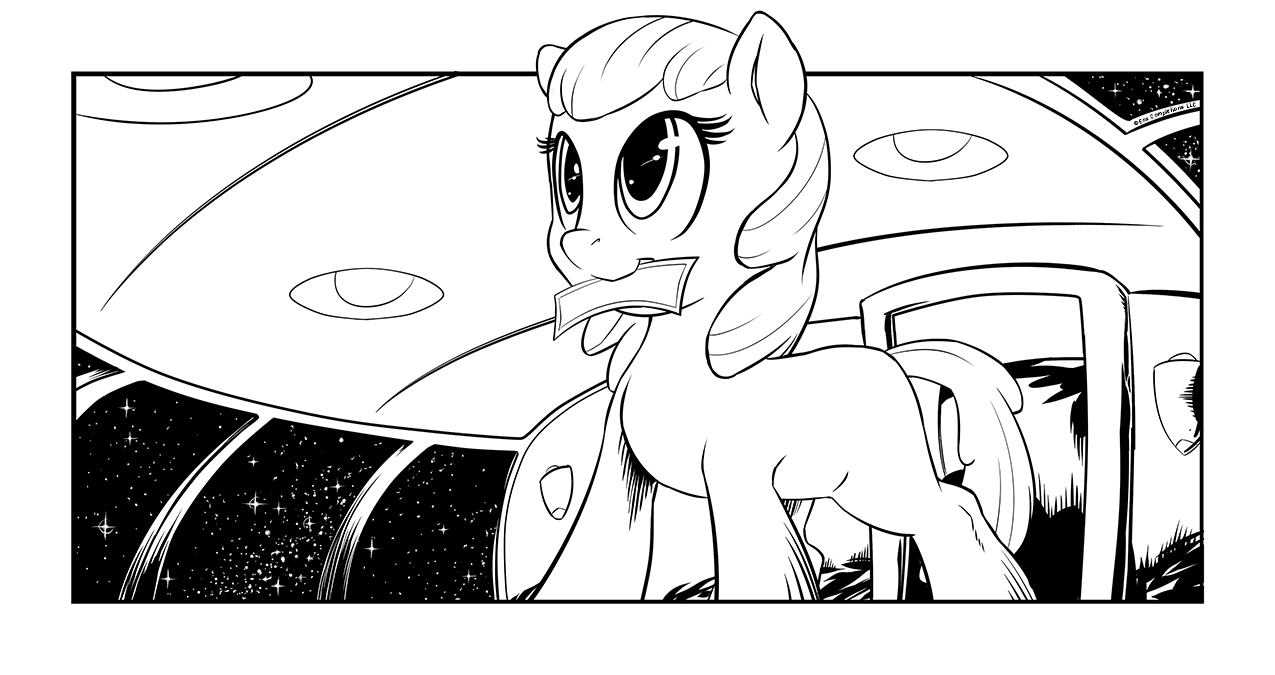
\includegraphics[width=0.9\linewidth]{image21.png}

\begin{intro}
Beyond the horizon, we will be together again.
\end{intro}

{\rt

``Oh, c'mon, you can't st---FZZT---rking right now!'' BAM BAM BAM! ``Hello? Hello? Test, test\dots onetwothree\dots''

``\dots''

``Okay, it seems like it's working. Very well, let's get started. First of all, my name is Watcher. My self imposed mission was to watch over the Wasteland, looking for lost ponies and groups of adventurers, hoping to eventually find those that carried the Elements of Harmony. Now, things are changing and I have friends that will help me with my task. I'm not alone anymore, and I finally have some time for doing things that I feel need to be done.

``And this is the reason why now I'm recording this tape and, just for this tale, I'm asking you to call me Mister Questioner. This is a story that could seem unimportant, or even silly, but it's about dreams, and memories. It's a story about two large, innocent pink eyes that couldn't see the horrors of our times and kept believing that somewhere, behind those ruined walls, inside the slave pens and even in the raiders' camps, everypony was still a pretty pony.

``And at the end of her journey, where the road met the ocean, the ghost foal that lost her mom finally found a place to rest. Sure, she was a little late, but I was told that when she finally accepted her fate, Puppy left with a smile.

``It was as if she was following an old postcard. She went down the Big 52, showing everyone she met what ponies had been in the past and what they could still be. Somehow changing the way they saw themselves, making them see a better past, and making them wish for a better tomorrow. She wasn't actually trying to change the world, or even to save lives, but that might have been why so many ponies took notice. Since she was no preacher but simply herself, it was easy to see that there was no fanaticism or weird ideals in her; just a little pony with large pink eyes that knew, for a fact, that no one could really be that evil.

``And this\dots this is what happened in the few months between Puppy's arrival at Emerald Shores and today.

``The ponies of Emerald Shores came back to the town shortly after the Wild Herd's defeat. When they arrived from the NCA, they found the graves on the hill and the remains of the crushed ferris wheel. Alas, what really startled them was that somepony had changed the name of the town on all the signs. Now the town is called Nightmare's Fall.

``The survivors of Ironworks started rebuilding the town, helped by their neighbours. Since the battle the settlement had a shortage of adult ponies, so the Rangers decided to settle in this town, making it their new headquarters. Not everypony was happy with this new situation, but the rangers proved themselves vital during the liberation of the town, and eventually even the most stubborn came to accept them.

``With Ivory Tower destroyed and Ironworks reduced at the shadow of its former self, Broccoli gathered all the ponies that didn't want to live in a ghost town or hadn't a home in which to live at all. The work in the fields improved greatly and the farmers diversified their crops, for the joy of the foals. Now they grow both broccoli and cabbage.

``The crater at Ivory Tower was filled by the seasonal rains and a small trading post has been built along the route between Broccoli and Rust Manor. The town is very small and lightly fortified, but it's growing fast and somepony is starting to build farms all around the lake. The town still doesn't have a name, but the traders call it The Hole.

``Rust Manor was attacked during the Enclave conflict. The town wasn't able to repel the attackers and the control tower was completely destroyed. Numerous ponies were killed, but the survivors are already beginning to rebuild their home. It won't be easy, but nothing is easy in the Wasteland.

``Sun City is still a war zone. The Sand Sweepers and a number of small bands are currently fighting each other to gain the control of the desert's gem. Since the Hired Hooves retreated from Sun City during the Enclave conflict and never came back, the settlement is still a dangerous place, avoided by almost every caravan. For those that dare to risk their lives, though, the inner town is full of old world technology that could make you rich for the rest of your life.

``Tunnel Town expanded on both sides of Sugartop Mountain and now it's the third largest town along the Big 52. The prices for using the tunnel have been cut considerably and the city began a service of long range patrols to keep at bay the groups of raiders and slavers along the Route in the town's territory.

``Salt Cube City is still the biggest city along the Big 52 and it has grown even more since the ghouls left the Dome. The Hired Hooves are expanding their influence even outside the Route, and have opened offices in the nearby towns. The Talons don't seem very happy with this policy, and tension between the two mercenary groups is rapidly growing.

``The Redtrotters didn't change very much. They stayed faithful to their tribal customs and are still charging the caravans that travel along their territory, but now foals don't have to pay the fee. This is not a big improvement, but the tribe has opened relations with the other settlements and they are actually trying to improve the safety of their part of the Route.

``The Applejack Rangers helped in reconstructing Ironworks, establishing their new base in the town's Stable. During the last battle at the Cave, all four of Ironworks's surviving paladins were dispatched to help with defending the place, and I had the opportunity to meet both Cold Shower and Scold. The battle was hard and Shower didn't survive it; she is now sleeping besides Gauss at Emerald Shores. Scold has grown distant after losing her. It seems that the old scribe is doomed to survive all his friends\dots A fate that I can easily understand.

``Happy and Jamie married and I was told that she is expecting. Since the marriage is quite a recent news, I think that they didn't expect to be celebrating again so soon. When asked what name they are planning to give the foal, Happy stated that she's still uncertain, but it won't be Puppysmiles.

``Molten Gold didn't stop his grave robbing career for long after the battle with the Nightmare. The ghoul left as soon as he recovered and sailed south on a steamboat, along with a group of adventurers. I haven't heard anything from him since then.

``SolOS and Pinkie 7 were actually able to become friends in the end. I was contacted by P7 a little after the first Enclave attacks. She was curious about this 'Questioner' Puppy was always talking about, so we had a chat, and even if I don't think I'm going to trust her or SolOS any time soon, I think that they aren't going to give us troubles for a while. She actually scared me a bit when she told me about her and SolOS's idea of programming a new A.I. and naming it Puppy.~SML. I hope that this was just a joke.

``Lonesome Pony recovered from his wounds and went back to Radio 52, keeping the Big 52 together with his encouraging speeches and all of his music. DJ Good Stuff is still working with him but when I tried asking when they were going to marry, both of them laughed at me. During the Enclave conflict Radio 52 kept broadcasting. It was small enough that the pegasi didn't bother to shut it down. The radio helped with organizing the defenses and boosted the morale of the defenders. It wasn't very much, but it was enough for those that fought during the conflict.

``Mister White trotted back to Salt Cube City. The loss of Sage Brush changed him deep inside, even if his sister never blamed him for it. After resigning his place of leadership, he became a traveling merchant, and as far as I know, he's still running along the Route, bartering every sort of merchandise. This is just a rumor, but it seems that one of his guards is a unicorn mare with a tower as a cutie mark. Maybe he didn't want to lose the opportunity to hire somepony that had the guts to spank a Nightmare, or he simply wanted to give a raider a second chance. After all, you gotta care, right?

``After Long Ears's demise, a new filly in her tribe got the Far Seer cutie mark, becoming the next shaman. I have no idea how their power works, but it seems to be some mix of powerful drugs and innate precognition. I just know that it is very tolling and quickly consumes the mare's body, so that a single pony sacrifices her life to help the tribe. A boon that brings a curse\dots

``There's still a pony that I never met in person, and I'm starting to doubt his actual existence. Puppy described him to me as the baddest evil villain ever. Count Horse Tile. I asked several travelers and caravan guards, but no one has been able to give me a single clue about this cruel noble pony\dots I guess his mystery will remain unsolved.

``Henrietta is still running from the Talons. It seems that there has never been good blood between them and the Firebrights, and the young griffon is keeping up the family tradition. I tried to talk with Gawdyna, to see if some sort of truce can be arranged. I hope that Henri will accept to parley. After all she was Puppy's best friend, and seeing the girl die because of a feud that she didn't even start is something I really don't want to see.

``The Wild Herd dispersed and fled to their outposts on the coast again. This time they suffered heavy losses, both in numbers and in pride, but everyone knows that they will come back one day. Hopefully, even if they once more strike the Big 52, it will be without the help of an army of robots, and that could be enough to let the good ponies sleep quietly, for the moment.

``The Lost Herd seems to be gone. With Sidekick's death, the last of those damned souls found peace at last, and finally Equestria will be able to forget one of the many horrors of the war. May those poor foals find a deserved rest in whatever awaits us past this life.

``So, this is the end of Puppy's story. Did she really change something along her path? Will her action matter in the long run? I have---sorry, I \emph{has} no idea, but I think I'll miss the way she talked, and the way she took everything so lightly. Another shard of the Equestria I loved is forever gone, but I still hope that I will live long enough to be able to see a filly like her again. But this time it won't be a ghost from the past, but a daughter of the present.

``And speaking of ghosts, the legend of the Ghost of the Big 52 is still alive, even if it seems more a Nightmare Night's tale than a real story. It's said that when the sun goes down and the moon is waning, a ghostly figure rides along the Route, silent like a shadow and swift like the wind. It looks for the souls of the wicked: slavers, raiders and the evildoers that lurk in darkness, waiting for easy prey. At least two groups of raiders were actually found dead along the route. They didn't show a single wound, their weapons were still fully loaded, and they were clearly ready to strike\dots but they died on the spot with no explanation. Killed by a presence that didn't leave a single clue. So, now I want to ask you one thing.

``Do you believe in ghosts?''

}

\horizonline

\englishdaytimeplace{4}{7:30 P.M.}{Downtown, Salt Cube City}

Sand Box turned the wheel left trying to make the airship fly against the wind, but it was an impossible task. \emph{Friend Force One} was losing pieces along the way since the take off, and two engines had already failed. He slammed his hoof down on the intercom and yelled: ``Soft Air, we need more power! We're getting pushed back by a damn nightly breeze! I don't know how, but give me more knots!''

The reply from the communication device had more in common with an electrocution than an actual conversation, but it was about the balloon losing gas and the engines catching fire.

Sand Box cursed, before talking again in the instrument. ``Okay don't worry, I've got a backup plan. We'll crash the airship here, so that the wind won't send us back to Salt Cube city!''

If the reply from the other side of the line was a complaint, it never reached Sand Box. In that very same moment the whole world decided to become pure light.

Just an endless, blinding, perfectly silent light that enveloped everything. There was no pain, and there was no fear. Just light.



\horizonline

\englishunknowndaytimeplace

When Sand Box opened his eyes again he had the unsettling feeling that there was absolutely nothing wrong. Nothing at all. He took his time to look for a moment around the flying deck, trying to understand what happened. Well, the wheel was still there, the sky was all starry, the commands were working, the lights were all lit\dots

``Wait a moment, the lights are all lit? There are stars outside? What the\dots''

Yes, the airship was working perfectly, and by perfectly it meant that the whole damn room seemed as new as the day it went out from the docks. The floor was shining, the commands were clean, the wheel was even waxed! And the windows! They were so clear that you could even see yourself inside th---

And Sand Box saw Sand Box. Surprise on his muzzle was giving way to realization. Slowly, he touched his face with a hoof. It was his real face, the one he had before becoming a ghoul! He was a pony again, he was\dots

Dead.

He was dead, this was the only possible reason for all of this. But if he was dead, why was he still on the ship? Was this some sort of afterlife punishment where he had to fly a ship forever, like the Flying Dutchmare? Were the others trapped forever on that thing with him? And why? He\dots he didn't want to fly forever, he had to see Agatha! She\dots she was waiting for him somewhere, he couldn't just\dots fly a stupid ship for the eternity!

FWEEEEET! A loud whistle interrupted Sand Box's shipwreck of desperation, making him turn toward the deck's entrance. A feminine voice announced her arrival while the door slammed open. ``Captain on the Bridge!''

A pink mare with a pink mane and big blue eyes appeared in front of the former ghoul. She was wearing a navy officer uniform and sported the largest smile Sand Box had ever seen on a pony. ``Miss\dots Minister Pie?''

Pinkie dismissed Sand Box with the wave of a hoof. ``Ah, call me Captain Pinkie, I don't like that ministry thing. It wasn't happy at all anyway.'' She started jumping in every corner of the bridge, giggling and yelling enthusiastically. ``Yay! I knew that this little filly was going to fly sooner or later! Oh, oh, look! Look at this! All the arrows on the panels are pink, exactly as I asked! It's\dots it's fantastic!''

The chief technician stood still with a confused expression on his muzzle, looking at the hyperactive pony touching everything while moving around at a speed that wasn't physically possible. ``I\dots Can I help you---''

Before Sand had the time to finish the question, he found himself staring into Pinkie's enormous blue eyes, nose to nose with her. ``Sure you can! They are all waiting for you in the lounge! Move that slow rump of yours and join the party! I'll get there as soon as I'm done having fun here!''

He nodded, slowly stepping back toward the door and never losing eye contact with Pinkie Pie. She was a little bit scary, especially from the point of view of a pony that had just been dead for less than ten minutes. Once on the stairs, he turned on his tail and rushed to the airship's recreational bridge.

The saloon wasn't crowded, but it was still quite populated, especially since Sand Box clearly recalled that aboard the \emph{Friend Force One} there were just four ponies when it took off. Now instead he counted eight guests.

It was easy to recognize Soft Air from his typical military technician jumpsuit, and Peach Blossom with her blooming peach flower cutie mark was easy to spot. The middle aged mare with the stethoscope had to be Dr. Get Well. Wow, she was quite a sight with all of her skin and muscles in their place. This left a griffon and four other ponies that Sand Box didn't recognize.

The griffon was sipping tea while reading a newspaper, sitting on a couch. He was wearing combat armor and had several weapons on him. Two of the ponies, a mare and a stallion, had the typical padded suit used under power armor and were standing side by side in front of a table with drinks and snacks. They didn't pay attention to the table anyway, being too occupied in nuzzling each other, seemingly at peace.

The third pony was sitting alone in front of a window, looking outside the ship. He sighed and shook his head, in his eyes was easy to read some sort of regret and resignation. As if he left too many things undone behind and wanted to go back. The fourth pony was a unicorn mare with a long cape. She had the Sand Sweepers traditional jewelry on her, maybe she was a dead farseer? The mare seemed different from the others, more a shadow than a real presence. She was also the one that trotted toward Sand Box when he stepped inside the room.

``Greetings. I see that Pinkie let you come down at last. I guess this means that we are ready to proceed. She should be here soon, unless she got lost again.''

Sand Box frowned. ``What is going on? Who is she? Who are you? Listen, I'm not a troublemaker, but I'd---'' He stopped talking when the mare approached a door and pulled it open. A pink foal with a blonde mane and two big pink eyes trotted inside the room.

Puppy still had her pretty silver ticket in her teeth. She didn't understand how exactly she arrived in that place, but it didn't matter. There were games, and treats, and it totally seemed like a super fancy party! It was everything she always dreamed, and it was full of ponies to boot! And a chicken!

Sand Box felt his heart sink in an icy grasp. Of all the ponies he was expecting to see, Puppysmiles was the last one. ``Oh, little one\dots I'm\dots I'm so sorry.'' How could this foal smile even in a moment like this? ``What happened? Who\dots how did you arrive here?''

Puppy tilted her head, unable to recognize the pony in front of her, but he seemed very nice, so it was all right. ``Hi mister pretty pony! I am Puppysmiles, and I am going to find my mom! A super nice skelly pony gave me this super fancy ticket and sent me here! And I was told that Mom was just over there, after the ride!'' She paused for a moment, checking the place. ``Ah, are we there yet?''

Sand Box blinked his eyes, trying to understand what the foal meant, but Long Ears came in his help, whispering in his ear, ``Her mother is dead.'' This only succeeded in making Sand's perplexity grow.

``You\dots you're happy to be dead?''

Puppy giggled. ``The nice skelly pony told me so, mister pretty pony! But I feel fine and I'm going to find Mom! This is, like, the best thing ever!''

``B-but\dots'' She was so\dots happy. And even if she was explained what was going on, what would have been the point of it? Sand Box smiled and nodded. ``Yes. Yes it is. Do you want to play something with the others until we arrive?''

In the meantime, the various ponies in the room had slowly gathered around Puppy. They were all looking at her with various degrees of perplexity or sadness. Cold Shower and Gauss approached the filly, Cold was the first to talk.

``I'm sorry that we had to fight you\dots I wish there was a better way.'' Gauss nodded for a moment, sighing deeply.

``Ah, why is everypony sad? Where are the pony games? I want to play hide and seek! Or pin the tail on the pony! And then I wanna dance, and\dots Oh, I hope the pony tail is pink! Pink is my super favorite color! I'm the bestest tail pinner ever!'' Puppy was already jumping on her hooves, trying to look beyond the small group of ponies.

Pinkie, now wearing a flight attendants uniform, followed Puppy through the door, and patted the foal on the head. ``I'm sorry Puppy, but there's no time for that! We've sailed through the Star Ocean, and now we have arrived! The ride ends here, fillies and gentlecolts! Thank you for choosing the afterlife airlines, and have a pleasant stay!'' Pinkie moved rapidly toward the door, opening it and revealing to the other ponies a wonderful landscape made of green hills and small ponds.

Small herds of ponies dotted the meadows, while pegasi sat on the clouds populating a wonderful blue sky. The passengers trotted outside the ship, staring in amazement at the view. It seemed like a dream come true. Here and there it was possible to see the roofs of some houses, and on the distant hills there was a large apple orchard.

Even Puppy was left speechless in front of the beauty of the landscape. Everything was perfect! The trees, the meadows, all the pretty ponies and the sunny sky! It\dots it was even better than Ponyville, it was so beautiful! The only thing that was missing was---

Puppysmiles froze for a second, her eyes staring into a small herd of ponies grazing on the borders of a daisy field. The smile on her face grew bigger and bigger as she galloped toward the ponies in the grass. One of the figures looked up and smiled at the incoming filly who was now crying with joy, unable to say anything but a single word.

``Mom!''




}

\pagestyle{chinese}
\chapter{后记}

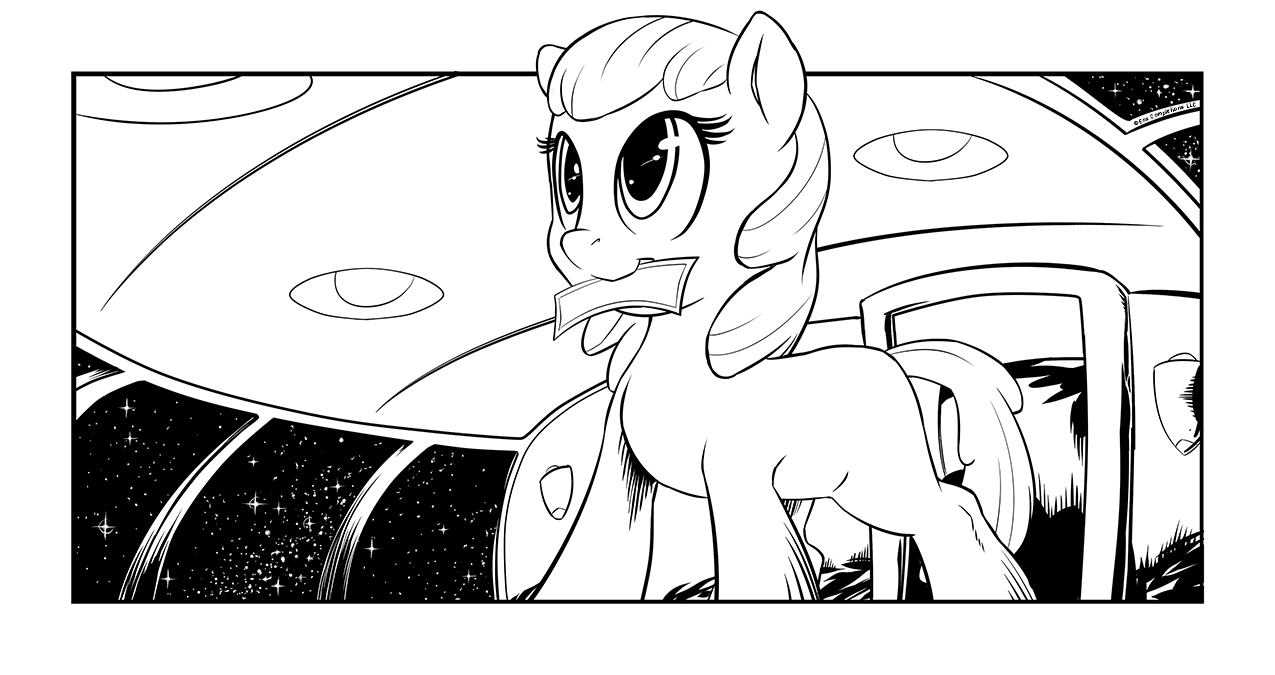
\includegraphics[width=0.9\linewidth]{image21.png}

\begin{intro}
    在那遥远的彼端,我们将再一次团聚。
\end{intro}

{\rt

「 拜托!别这样……滋滋……给我工作啊!」咣!咣!咣!「喂,喂,喂……测试测试……一二三……

「……

「好了,看起来没问题了,很好,我们开始吧,首先,我的名字叫守望者,我给自己的任务是守护整个废土,寻找那些在冒险中迷失的小马,希望能够找到那些带着谐律之源美德的小马。不过现在不一样了,我有很多朋友帮我的忙,我再也不孤单了,所以我终于有时间做我之前早应该做的事情。

「这就是我录这个磁带的原因,不过这一次,我希望你们叫我『提问者』。这个故事看起来不是那么重要,甚至有些傻里傻气,不过这个故事是关于梦与回忆的故事,是一个关于一双天真无邪的大眼睛的故事,那是一双即使看到现实的残酷,也坚信在这这片废墟之上,在那些奴隶营之中,甚至那些强盗的营地里面,每一个小马都还是漂漂马的大眼睛。

「而在她旅途的终点,当道路终于将她带到海边,迷失的小幽灵终于找到了安息之地。虽然她安息得稍微有那么一点迟,不过大家都说,她最终接受自己的命运的时候,是含笑离去的。

「这个小雌驹就像是来自战前的旧海报一样,她给52号国道上遇到的每一位小马带去了明媚的阳光,改变了他们如何看自己的方式,让他们看到一条更美好的道路,让他们更加期待明天。她并没有想要改变这个世界,或者拯救生命,但是她却引起了很多小马的关注。她自己并没有想当一个布道者,因为她显然不属于任何宗教或者派系也没有什么奇怪想法。她只是一个孩子,一个有着一对大大的粉色双眸的小孩子,她坚信着,众生天性本善。

「这些,这些就是帕比到达翡翠海岸之后又发生的故事。

「在野牛帮被击退之后,翡翠海岸的居民回到了他们的城镇。当他们从NCA过来的时候,他们发现那海岸边山丘上的新墓碑,还有倒塌的摩天轮。那景象确实让他们大吃一惊,在那之后不知道谁改了那个小镇的名字,现在那里叫做梦魇陨落。

「在新邻居的帮助下,铁砧镇的幸存者开始重建小镇,既然这里缺乏成年马,所以铁骑卫决定在这里定居下来,把这里当做他们的新总部。虽然不是所有小马都满意,不过铁骑卫用行动证明了自己对小镇的价值,之后就算最保守的小马也接受了他们。

「象牙塔和铁砧镇被摧毁之后,花椰菜那里迎接了无数流离失所的难民,那里的田地被扩大了好几倍,而且那里的农夫也提高了他们种田的技术。为了孩子们的快乐,他们现在不只种花椰菜,还种起了卷心菜。

「象牙塔现在的深坑已经被雨季的雨水填满,形成一个小湖,很多在花椰菜和铁锈庄园之间来去的行商在这里建立了一个临时落脚点,这里扩张得很快速,虽然到现在都没有一个名字,不过已经有一些行商叫这里『弹坑镇』。

「铁锈庄园在之后的英克雷入侵中饱受摧残,那里的机场控制塔都被炸毁了,很多小马都在战斗中牺牲。但是幸存者已经开始重建他们的家园,虽然那并不轻松,但是在废土之上没有什么事情是轻松的。

「太阳城现在还是个战区,因为聘蹄在英克雷入侵中离开了太阳城并且再也没回来,所以现在清砂帮和很多小帮派在都争夺这个沙漠明珠的控制权,这里还是个危险的地方,很多商队都绕道而行。不过对于那些敢于冒险的小马,城里随处可见的战前科技会让他们一夜暴富。

「隧道镇两边的城镇都扩张了好几倍,现在是52号国道第三大城市。隧道镇的隧道通行费现在变得很便宜,而且城市的卫兵开始在沿途进行巡逻,赶走了领土上所有的强盗和奴隶贩子。

「盐块城依然是52号国道最大的城市,而在那些尸鬼离开圆顶之后,城市更加发展壮大了。聘蹄的名声甚至远扬52国道之外,而且开始接受其它城市的任务了,虽然鹰爪并不太喜欢他们的新政策,不过两个佣兵势力之间的紧张关系正在慢慢升温。

「赤兔是改变最少的,他们依然保持着部族的传统,依然在他们的领土上游牧,不过幸运的时候,他们的孩子们可以自由地玩耍了。另外虽然不是什么大改变,部族现在也开始和其它城市合作了,并且在道路沿途设立定居点,让道路现在变得更安全。

「至于野牛帮,他们似乎在重创之后消声觅迹了,不过大家都知道他们总有一天还会卷土重来。但即使他们下一次再袭击52号国道,也不会有机器大军的帮助了,所以很长一段时间之内,小马们晚上都可以安心入睡。

「那些帮助铁砧镇重建的阿杰铁骑卫把他们的新基地建立在了铁砧镇的避难厩里面。在守护巢穴的战斗中,四位幸存的帕拉丁都来帮我守护这里,我有幸见到了冷浴和诘责,很可惜冷浴在那场恶战之中壮烈牺牲,她现在和她的朋友高斯一起长眠在翡翠海岸。诘责在失去她之后更加孤僻了,好像老书记官认为自己才是给朋友带来厄运的小马……我深深地理解他……

「乐乐和老枪结婚了,而且听说她怀孕了,这是最近才听到的消息,不过他们似乎并不想这么快就大张旗鼓地庆祝,不过我问起他们打算给小孩起什么名字的时候,乐乐看起来还没拿定主意,不过肯定不会是快乐帕比。

「融金在梦魇一战之后并没有停下他的传奇旅程,那尸鬼在康复之后就马上登上一艘航向南方的船,和一群冒险家一起探索新的大陆,不过在那之后我就没听说过他的传闻了。

「旭日系统和萍琪七号最后真的变成朋友了。我在第一次英克雷进攻之后联系到了P7,她很好奇这个帕比经常提到的『提问者』,所以我们聊了很久,虽然我还是不太信任她或者旭日OS,但是我觉得他们至少一段时间内不会给我们带来麻烦。不过她最后跟我说的一件事把我吓坏了,她似乎打算和旭日OS共同编写一个新的自律智能,并且起名为欢乐帕比\footnote{欢乐帕比:Puppy.~SML}……我希望这最好是个玩笑。

「孤狼在伤好之后继续经营他的52电台,继续用他的声音和音乐鼓舞着52号国道上的每一位居民,DJ好货也和他一同工作,不过我问他们打算什么时候结婚的时候,他们都在嘲笑我。在英克雷袭击中,52电台也一直持续工作,这个电台帮助52号国道组织起一次又一次反攻,并且极大地鼓舞了小马们的斗志,虽然并不是很大的帮助,但是足够让整个52号国道的居民打败了入侵者。

「白先生回到了盐块城之后,灌木的去世似乎让他受伤很深,即使她的妹妹并没有责怪他,但是他却不停地自责。之后他放弃了他的领导位置,变成一个旅行商,他现在依然在52号国道大路上来回行商贩卖着各种货物。不过有个传闻,据说他的秘书是一个有着白塔可爱标记的独角兽雌驹。或许他觉得雇佣一个有胆量打梦魇之月屁股的雌驹是一件很拉风的事,或许他只是想给一个强盗第二次机会……对吧?

「在长耳去世之后,她们部落又有一个新雌驹得到了先知的可爱标记。我不知道她们那神秘魔法是怎么弄的,不过用六种强力毒品混合出的迷幻药绝对会很快摧毁一个雌驹的身体,所以每次都需要有一个小马为部族而献身。

「赫瑞塔依然在四处躲藏着鹰爪的追杀,看起来他们和火红家族之的裂隙暂时无法弥补。那只年轻的狮鹫继续着家族的传统,我和高纳德聊过,看看能不能商讨出一个停战协议,毕竟她是帕比最好的朋友,如果看到她什么大事都没有做成就死于鹰爪的追杀,那实在太可惜了。

「幽灵羊群似乎已经完全消失了,在小跟班死后,每一个可怜的小灵魂似乎都终于安息了,小马国也可以愈合那场战争造成的众多伤痕之一,希望那些小家伙在来世之中找到他们的归宿。

「不过还有一个小马我从来没有见过,而且我甚至开始怀疑他是否存在,帕比跟我说他可是……她所见过的最坏坏蛋,马尾伯爵,我问了很多旅者和车队卫兵,不过看起来没有谁对这个残酷的贵族小马有什么印象……我觉得或许将是个永远无法解开的谜团。

「好了,这就是帕比故事的结局了,她真的在旅途之中改变了什么吗?她这场长长的冒险真的有意义吗?抱歉,我也不知道,不过我想我会怀念她的,在她看来,一切都如此简单。随着她的去世,另一片来自战前小马国的碎片也永远随风而逝。不过我希望今后有一天能够再次见到和她一样天真无邪的孩子,希望这一次不是来自过去的幽灵,而是某对真实夫妻的女儿。

「说到幽灵,52号国道的幽灵传说依然在继续,而且现在听起来更像是梦魇夜的鬼故事。据说在太阳落山,月亮升起来之后,一个无声的幽灵会随风在大路上游荡,它会夺走那些坏孩子的灵魂。那些奴隶贩子,那些强盗,甚至那些心怀恶意的家伙,他们身上没有一点伤口,武器依然上膛,但是他们却都已经死了,完全不知道被什么东西袭击,一点线索都没有。所以,我只想问你一件事。

「你相信幽灵么?」

}

\horizonline

\daytimeplace{4}{7:30 PM}{闹市区,盐块城}{Downtown, Salt Cube City}

沙盒用力按着船舵,让飞空艇迎风飞行,不过看起来完全不可能。友谊一号正在慢慢地失去他们起飞的速度,两个引擎已经熄火了,尸鬼用蹄子猛砸内部通话系统的开关,然后喊道:「软气,我们需要更多动力!我们正在被夜风吹回去!我不知道怎么做,不过再快几节行不行!」

话筒里传来带着静电沙沙声的回答,听起来似乎是气球正在漏气还有引擎起火啥的。

沙盒咒骂着,然后再一次怒吼起来。

「好了,别担心,我还有另外一个计划,我们让这个空艇就在这里坠毁,这样夜风就不会把我们吹回盐块城了!」

不过那一边的回答沙盒并没有听到,因为这个时候整个世界都被一道亮光洗白了。

无穷无尽的炫目光明掩盖了一切,没有痛苦,没有恐惧,只有光明。

\horizonline

\unknowndaytimeplace

当沙盒再一次睁开眼睛的时候,他微妙地感觉到有什么不对劲——应该说没有任何『不对劲』。他环视着舰桥,想搞明白到底出了什么事。船舵还在那里,外面的天空繁星闪闪,指令舱一切正常,灯泡也全亮……{}

「等等……灯泡怎么全好了?外面的星星是怎么回事?到底是……」

没错,飞艇运行得非常良好,比那整个拱顶塌下来,它飞出空港的时候都要好!地板闪闪发光,指令台擦得锃亮,甚至舵上还打了蜡!还有窗户,都擦得如此洁净,甚至可以看得见自己的……{}

然后沙盒看到了自己那吃惊到发傻的表情,他慢慢的伸出蹄子碰了碰自己,那是……他自己的脸,真正的脸,在他变成尸鬼之前的脸!他又是小马了!他……{}

死了。

他死了,这是一切唯一合理的解释。但如果他死了,为什么还在这艘船上?难道是某种死后世界的惩罚,他必须永远开着这艘飞艇,就像是加勒比海马一样?其他小马也和他一样永远困在这艘船上了么?为什么?他才不要永远飞这东西!他要见阿加莎!她……她肯定某处等待着他……他不能就这样……就这样开着一艘破船到处漂流!

一声明亮的口哨打断了沙盒的鬼船猜想,把他的视线拉回了舰桥入口,一只雌驹推开舱门大喊,她的嗓门又尖又高,刺得沙盒鬃毛都竖了起来。

「船长驾临舰桥\footnote{船长驾临舰桥(CAPTAIN ON THE BRIDGE):星际迷航名句}!」

有双蓝色大眼睛和粉色卷毛的粉色雌驹蹦跶到了前尸鬼面前,她穿着一身海军军官制服,脸上还带着沙盒从来没见过的大大笑容。

「萍……额……派部长?」

萍琪并拢双蹄行了一个军礼,「喏,叫人家萍琪船长就是,才不喜欢那些政治杂务……一点都不有趣!」年轻的雌驹在舰桥上蹦来蹦去,疯疯癫癫地咯咯笑着打滚,「耶!我就知道这孩子迟早能飞上天!哦哦哦哦!你看这个,所有的仪表盘都是粉色,和我要的一样!简直太妙了!」

首席技师满脸莫名其妙地看着那神经兮兮的雌驹用他眼睛都跟不上的速度在船上碰这碰那。

「呃……有什么我可以效劳的么?」

还没把话说完,沙盒就发现萍琪已经跳到了他面前,自己正在和萍琪那对蓝蓝的眼睛小眼瞪大眼。

「当然有!他们早就在沙龙等亲了!快去下面参加派对吧!等我在这儿玩够了就下去!」

那公马点点头,一边慢慢后退到门口,一边紧紧盯着萍琪。感觉她稍微有点可怕,特别是在一个刚刚死了没有十分钟的小马眼里。等蹄子踩上楼梯的时候,他急忙调转尾巴飞快地离开舰桥。

下面的沙龙虽然不是挤得满满当当,但是依然算是热闹非凡。沙盒明明记得友谊一号起飞的时候只载了四个乘客,但是现在他却看到八个宾客。

他很容易就认出了穿着飞行员制服的软气,桃花的那个绽放桃花可爱标记也很好认,在他们俩身边的那个中年雌驹应该就是好好医生,不得不说,她的皮肉都在身上的时候真的很有风韵。而另外一边的那个狮鹫和另外四只小马,沙盒就不认识了。

狮鹫正坐在沙发里面看着报纸喝茶,他穿着一件防弹衣,上面挂着好几把武器。另外两只小马——一公一母马,都穿着动力装甲下面的战术衬垫服,正在肩并肩站在桌子旁边吃着点心。他们其实并不太关心桌子上的东西,而是时不时地互相磨蹭着对方,看起来相当恩爱。

第三只小马则坐在窗边,忧心忡忡地看着窗外,一个劲儿地叹气。他的眼神中有太多的后悔和留念,看起来他对世界还有太多眷恋,并不想走。而第四只小马是穿着长披风的独角兽雌驹,她带着清砂帮的珠宝饰物,或许她是个先知什么的?那个雌驹看起来和其他小马完全不同,似乎只是个影子而不是真实的存在。不过她看到沙盒走进屋子里面就立刻站起来迎接他。

「您好,看起来萍琪最后还是把你叫下来了,看起来我们已经可以继续了……我想她很快就会来这里了,除非她又迷路了。」

沙盒皱起了眉头,「继续什么?她是谁,你又是谁?我说,我不是来找麻烦的,但是……」他的话被一阵小小的蹄声打断,一只有着大大粉色双眼,金色鬃毛的粉色小雌驹跑进屋子里面。

帕比在嘴里紧紧衔着她的那张银色机票,她不太清楚自己怎么来到这个地方的,不过没关系,这里有游戏,有吃的,看起来绝对是个超级华丽的派对!这是她一直梦想的一切,而且这里面都是小马,还有个小鸡!

沙盒觉得自己的心开始往下沉,在死后想见到的所有小马里面,他最不想见到的就是快乐帕比。「哦,小家伙……我……我……很抱歉……」为什么这孩子现在还能露出这样灿烂的微笑?「发生什么了?是谁……你怎么到这里的?」

帕比微微歪着头,似乎没有认出来面前的是谁,不过他看起来很友好所以没关系。

「嗨!漂漂马先生!我叫快乐帕比!我马上要见到妈妈了!一个超级好的骷髅马给了我这张超级厉害的机票然后把我送过来了!而且他说我马上就可以看到妈妈,就在降落之后!」小雌驹顿了顿,看了看窗外。「我们还没到么?」

沙盒眨了眨眼睛,想明白那孩子到底在说什么,不过长耳走过来和他咬耳朵,「她的妈妈已经死了……」但是这只是让沙盒更混乱了。

「你……你死了很高兴?」

帕比咯咯笑着,「那个骷髅马也这么问我,不过我现在觉得很开心因为我马上就能见到妈妈了,这就像是……像是……最好最好的事情!」

「但……但是……」她是那么快乐,即使是她已经知道将要发生什么,不过,有什么好不开心的么?沙盒想到这里微笑地掉了点头。

「对,没错,降落之前你想和我们玩游戏吗?」

在他们聊天的时候,房间里面的小马已经慢慢聚集到了帕比身边,他们看着那小雌驹,视线里都带着一丝歉意和一丝悔意。冷浴和高斯走到小雌驹身边,那母马先开口了。「很抱歉我们必须和你一战……我真希望我们有更好的办法……」高斯也点了点头,深深叹了口气。

「哎?为啥大家都那么伤心?为什么不玩游戏?我要玩捉迷藏!或者钉马尾!或者大家一起来跳舞也可以!哦哦哦……钉马尾的马尾要粉色的!因为粉色是我最喜欢的颜色!我可是最厉害的钉马尾大师!」看到这么多小马围过来,帕比乐得一蹦三尺高。

不知什么时候换上了一件空姐制服的萍琪从帕比进来的那个门走了过来,拍了拍小雌驹的头,「很抱歉帕比,没时间做游戏啦!因为我们已经到达了星之海的彼岸!现在我们已经降落啦!旅途到此结束,女士们,先生们!感谢你们选择天堂航班!祝你们旅途愉快!」粉色雌驹飞快地跑到门口打开舱门,而舱门外是一片绿茵盎然的境外桃源美景。

一群群小马在草地上悠闲的散步,天马坐在蔚蓝天空中的朵朵白云上。飞船的旅客登机梯伸展下去,落在了这片美丽的大地上。这里看起来就像是美梦成真一样,远处还能看到一片片美丽的果园和一幢幢平整的房屋。

即使是帕比也被面前的美景惊得说不出话来,那些树木,那些草地,还有那么多漂漂小马和美丽的蔚蓝天空……这比……这比小马镇都要棒!这里如此美妙,唯一缺的就是……

帕比愣了一下,她望着那一小群朝飞空艇走来的小马,脸上的微笑越来越灿烂。她跳下飞船飞奔在草地上。迎面飞奔而来迎接她的,是一只同样喜极而泣的雌驹。帕比开心得什么都说不出来,唯一能大声喊出来的,就是——

「妈咪!」





\chapter{Acknowledgements}

% NOTE: pagestyle 放在 english 环境外面,否则无作用

\pagestyle{english}

{\englinespread

\begin{center}
    This fanfiction is based on \emph{Fallout: Equestria} by Kkat.    
\end{center}

\section*{Author}

\begin{center}
    Mimezinga
\end{center}

\section*{Cover by}

\begin{center}
    LimreiArt\footnote{\url{https://www.deviantart.com/limreiart/art/Pink-Eyes-513444372}}
\end{center}

\section*{Illustrations by}

\begin{center}
    Boiler3\footnote{\url{https://www.deviantart.com/boiler3/}}
\end{center}

\section*{Speical Thanks for Writing}

\begin{table}[H]
    \centering
    \begin{tabular}{ccc}
        Nyerguds & Damhoof & Easteu \\
        Aerondight & Arcane Scroll & Palacioskw \\
        Anonsamurai & & \\
    \end{tabular}
\end{table}

\section*{Typeset by}

\begin{center}
    RandomQuantum
\end{center}

\section*{Special Thanks for Typesetting}

\begin{table}[H]
    \centering
    
    \begin{center}
    Chinese \TeX{} Society\footnotemark and C\TeX{} Fourm\footnotemark
    \end{center}
  
    \begin{tabular}{rl}
        Ruixi Zhang & \texttt{@RuixiZhang42} \\
        Xiangdong Zeng & \texttt{@stone-zeng} \\
        Zeping Lee & \texttt{@zepinglee} \\
        & \texttt{@muzimuzhi} \\
        ChenCheng Huang & \texttt{@Liam0205} \\
    \end{tabular}
\end{table}

\addtocounter{footnote}{-2} % -2
\stepcounter{footnote}\footnotetext{\url{https://github.com/CTeX-org}}
\stepcounter{footnote}\footnotetext{\url{https://github.com/CTeX-org/forum/}}



\section*{Links}

\begin{itemize}
    \item Published on Fimfiction: \url{https://www.fimfiction.net/story/931/fallout-equestria-pink-eyes}
    \item English Ducument: \url{http://book.fallout-equestria.com/forum/viewtopic.php?f=3\&t=342}
    \item This Project on GitHub: \url{https://github.com/Ranqumn/FoE_pink_eyes_publish}
\end{itemize}

}

% --------------------

\chapter{致谢}

\pagestyle{chinese}

\section*{译者}

\begin{center}
    MadCatMKII
\end{center}

\section*{初版制作}

\begin{table}[H]
    \centering
    \begin{tabular}{rl}
        NightScream & 校对 \\
        ShadowDumb & 校对\ 排版 \\
        NightlySound & 润色 \\
    \end{tabular}
\end{table}

\section*{特别感谢}

\begin{center}
    立冬 \quad Onisk
\end{center}

\section*{重排版制作}

\begin{center}
    RandomQuantum
\end{center}

\section*{专业排版特别感谢}

\begin{table}[H]
    \centering

    \begin{center}
    中文 \TeX{} 学会\footnotemark 与 C\TeX{} 论坛\footnotemark
    \end{center}

    \begin{tabular}{rl}
        张瑞熹 & \texttt{@RuixiZhang42} \\
        曾祥东 & \texttt{@stone-zeng} \\
        & \texttt{@muzimuzhi} \\
        Zeping Lee & \texttt{@zepinglee} \\
        黄晨成 & \texttt{@Liam0205} \\
    \end{tabular}
\end{table}

\addtocounter{footnote}{-2} % -2
\stepcounter{footnote}\footnotetext{\url{https://github.com/CTeX-org}}
\stepcounter{footnote}\footnotetext{\url{https://github.com/CTeX-org/forum/}}


\section*{相关链接}

\begin{itemize}
    \item 作者原文地址 \url{https://www.fimfiction.net/story/931/fallout-equestria-pink-eyes}
    \item 英文电子文档 \url{http://book.fallout-equestria.com/forum/viewtopic.php?f=3\&t=342}
    \item 译文首发地址 \url{http://blog.sina.com.cn/u/3149389173}
    \item 完整译文地址 \url{https://fimtale.com/t/2387\#/radiant-ponies-pink-eyes}
    \item 印刷初版首发地址 \url{https://www.equestriacn.com/}
    \item 重排版项目地址 \url{https://github.com/Ranqumn/FoE_pink_eyes_publish}
    \item 封面首发地址 \url{https://www.deviantart.com/limreiart/art/Pink-Eyes-513444372}
    \item 插图 Boiler3 \url{https://www.deviantart.com/boiler3/}
\end{itemize}

% TODO: 添加地址


\clearpage

% ---------

% 手动调整

\fancyhf{} % 清空

\fancyhead[LE,RO]{\thepage}

\fancyhead[LO]{\sffamily \uppercase{Acknowledgements}} % 奇数页  \leftmark = 章节名称
\fancyhead[RE]{\sffamily \uppercase{Fallout Equestria: Pink Eyes}} % 偶数页

% 

~\vfill

\section*{The Last Special Thanks}

\begin{center}

    \Large You

\end{center}

~\vfill

\clearpage


~\vfill

\begin{center}

\begin{englishpar}
    \sout{Press any key to skip credits}
    
    (This function has not been provided yet)
\end{englishpar}

\CJKsout{按任意键跳过制作人员列表}

(暂不支持该功能)

\begin{englishpar}
    Thank you for playing \emph{Fallout Equestria: Pink Eyes}
\end{englishpar}

感谢您玩赏
\end{center}

~\vfill

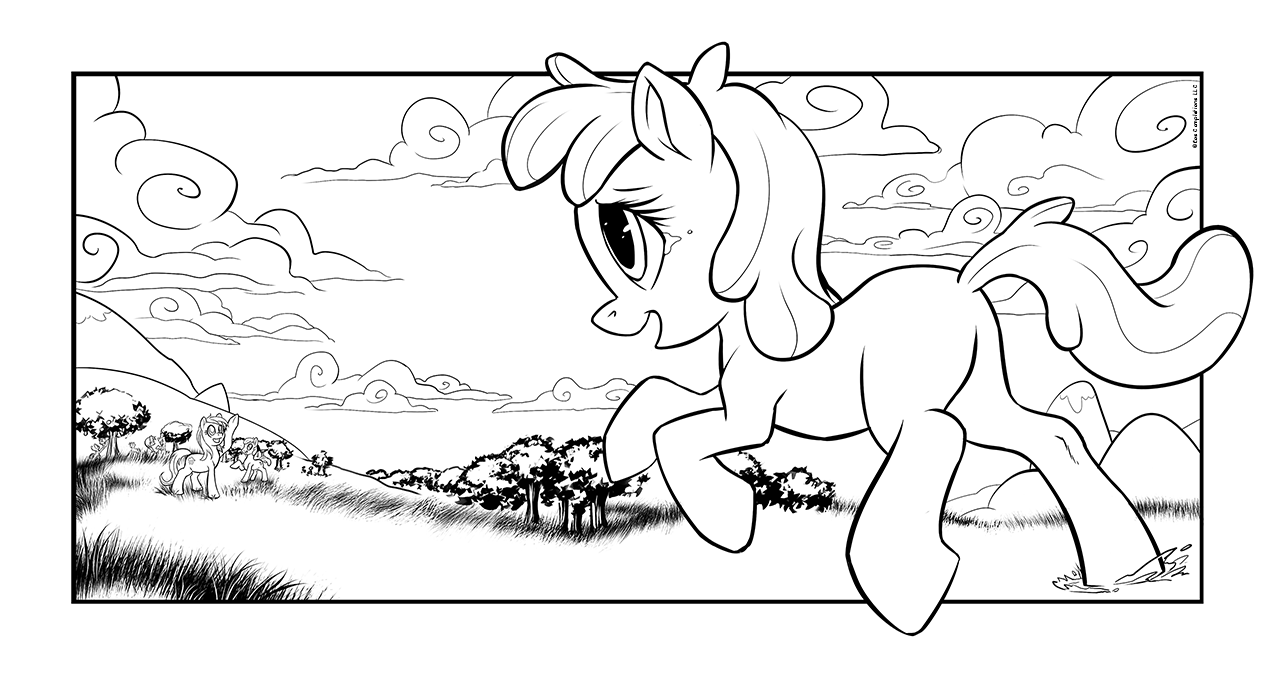
\includegraphics[width=0.9\linewidth]{image22.png}

\begin{motto}
    Do you believe in ghosts?

    你相信幽灵吗?
\end{motto}






\end{document}

